%%%%%%%%%%%%%%%%%%%% author.tex %%%%%%%%%%%%%%%%%%%%%%%%%%%%%%%%%%%
%
% sample root file for your "contribution" to a contributed volume
%
% Use this file as a template for your own input.
%
%%%%%%%%%%%%%%%% Springer %%%%%%%%%%%%%%%%%%%%%%%%%%%%%%%%%%


% RECOMMENDED %%%%%%%%%%%%%%%%%%%%%%%%%%%%%%%%%%%%%%%%%%%%%%%%%%%
%\documentclass[graybox]{svmult}
\documentclass[deutsch]{svmult}
\usepackage{import}
% choose options for [] as required from the list
% in the Reference Guide

\usepackage{type1cm}        % activate if the above 3 fonts are
                            % not available on your system
%
\usepackage{makeidx}         % allows index generation
\usepackage{graphicx}        % standard LaTeX graphics tool
                             % when including figure files
\usepackage{transparent}
\usepackage{multicol}        % used for the two-column index
\usepackage[bottom]{footmisc}% places footnotes at page bottom


\usepackage{placeins} % for FloatBarrier

\usepackage{newtxtext}       % 
\usepackage{newtxmath}       % selects Times Roman as basic font
\usepackage{mathtools} %matrix* environment which allows alignment specifier

\usepackage{comment}
\usepackage{capt-of} % side by side figures in a figure-env need captionof to generate captions


% My Own Macros
\newcommand{\refFig}[1]{\figurename~\ref{fig:#1}}
\newcommand{\refEq}[1]{(\ref{eq:#1})}
\newcommand{\sus}[1]{\protect\raisebox{-0.33ex}{\scriptsize #1}} %subscript index in text-mode

% Symbols with Prime (subscript too low otherwise)
\newcommand{\aXDPrime}{a_{x\mathrm{d}}\hspace{-0.8em}^\prime\hspace{0.52em}}
\newcommand{\kappaDPrime}{\kappa_\mathrm{d}\hspace{-0.39em}^\prime\hspace{0.1em}}
\newcommand{\deltaDPrime}{\delta_\mathrm{d}\hspace{-0.39em}^\prime\hspace{0.1em}}
\newcommand{\tauXDPrime}{\tau_{x\mathrm{d}}\hspace{-0.8em}^\prime\hspace{0.52em}}


\newcommand{\aXD}{a_{x\mathrm{d}}}
\newcommand{\aXT}{a_{x,\mathrm{traj}}}
\newcommand{\vXT}{v_{x,\mathrm{traj}}}


\definecolor{light-gray}{gray}{0.7}


\usepackage{pgfplots}
\usepackage{tikz} 

\newlength\figureheight 
\newlength\figurewidth 
\setlength\figureheight{6cm} 
\setlength\figurewidth{16cm}

%%%%%%%%%% End of our changes

% see the list of further useful packages
% in the Reference Guide

\makeindex             % used for the subject index
                       % please use the style svind.ist with
                       % your makeindex program

%%%%%%%%%%%%%%%%%%%%%%%%%%%%%%%%%%%%%%%%%%%%%%%%%%%%%%%%%%%%%%%%%%%%%%%%%%%%%%%%%%%%%%%%%

\begin{document}


\title*{Optimal Trajectory Planning}
% Use \titlerunning{Short Title} for an abbreviated version of
% your contribution title if the original one is too long
\author{Moritz Werling}
% Use \authorrunning{Short Title} for an abbreviated version of
% your contribution title if the original one is too long
\institute{Moritz Werling \at BMW Group,  München and Karlsruhe Institut of Technology,  Karlsruhe, \email{moritz.werling@bmw.de}}
%
% Use the package "url.sty" to avoid
% problems with special characters
% used in your e-mail or web address
%
\maketitle
\abstract{Neue vernetzte Fahrerassistenzfunktionen mit simultaner Längs- und Querführung  bei gleichzeitig  unterschiedlicher Einbindung des Fahrers in die Fahraufgabe stellen eine große Herausforderung dar. Eine aus einer überlagerten Fahrstrategie vorgegebene Trajektorie für die Fahrzeugbewegung mit dem Ziel der Erfüllung einer bestimmten Längs- und Querführungsaufgabe soll hierbei in Aktuatorstellgrößen für das Lenk-, Antriebs- und Bremssystem überführt werden. Wegen des zunehmend größeren Betriebsbereichs hinsichtlich Fahrgeschwindigkeit und Kraftschlussausnutzung in Längs- und Querrichtung sowie des zunehmenden Autonomiegrades ist ein integrierter Ansatz vorteilhaft der alle fahraktiven Fahrerassistenzfunktionen, also Parkier-, Komfort und Fahrsicherheitsfunktionen betrachtet. Der Ansatz soll geeignet sein, sowohl Einzelfunktionen der Quer- oder Längsführung als auch Funktionen mit kombinierter Längs-und Querführung mit jeweils unterschiedlichem Autonomiegrad abzudecken. Eine wesentliche Herausforderung stellt hierbei die Gestaltung der Kooperation mit dem Fahrer dar, die sowohl autonomes als auch kooperatives Fahren und die Übergänge zum manuellen Fahren z.~B. zum Aktivieren oder Deaktivieren von Funktionen durch den Fahrer adressieren soll.\\ Dieses Kapitel beschreibt detailliert einen in der industriellen Praxis bewährten Ansatz zur integrierten Quer- und Längsführung. Der Ansatz basiert auf einer funktionsübergreifend einheitlichen kaskadierten hierarchischen Reglerstruktur bei der in Anlehnung an das Drei-Ebenen-Modell die  Aufteilung der Regelungsaufgabe auf die Bahn- und Fahrzeugführungsebene erfolgt. Auf Grundlage der Fahrstrategie und der gewählten Assistenzfunktion gibt eine Trajektorienplanung einen bestimmten Sollverlauf für die Fahrzeugbewegung in Längs- und Querrichtung vor. Die Einregelung des Sollverlaufs unter besonderer Berücksichtigung der Interaktion mit dem Fahrer und Überführung in Stellgrößen für die Lenk-, Brems- und Antriebsaktuatorik erfolgt auf Grundlage der Methoden der linearen, robusten bzw. adaptiven modellbasierten Regelungstheorie und der Robotik. Grundlage für den regelungstechnischen Entwurf sind hinsichtlich der Stuktur sehr gut bekannte mathematische Modelle die die ebene Längs-, Quer- und Gierbewegung des Fahrzeugs, der Lenkung und der Bewegung relativ zu einer vorgegebenen Trajektorie beschreiben. Wegen der beladungs- und reibwertabhängigen Ungenauigkeit der mathematischen Modelle werden diese um entsprechende Unsicherheitsmodelle erweitert.  Eine mathematische Beschreibung des Betriebsbereiches, der Anforderungen hinsichtlich Regelgüte, Stabilität und Robustheit des Führungs- und Störübertragungsverhaltens werden formuliert und für exemplarische Assistenzfunktionen anhand von Experimenten gezeigt.
}

%und die Integration verschiedener Einzelfunktionen der Längs- und/oder Querführung
\section{Einleitung}\label{S:Intro}

Moderne Fahrsicherheits-, Fahrkomfort- oder Parkiersysteme wie Kollisionsvermeidung, Ausweich-, Nothalteassistenz, Spurhalteunterstützung, Stauassistenz und ferngesteuertes Einparken werden eingesetzt, um den Fahrer von seiner Fahraufgabe zu entlasten und das Fahren sicherer und komfortabler zu gestalten. 

In der industriellen Entwicklung der Fahrerassistenz in den beiden letzten Dekaden wurden in der Regel Einzelfunktionen mit begrenztem funktionalem Umfang und Betriebsbereich sowie individuellen Sicherheitskonzepten, Funktions-, Bordnetz- und Softwarearchitektur in Kooperationsmodellen mit unterschiedlichem Funktionsschnitt zwischen Fahrzeugherstellern und Lieferanten entwickelt.  
Zu Beginn legitim und vorteilhaft wegen der sehr unterschiedlichen Betriebsbereiche und sich abgrenzender Fahrfunktionen bzgl. Verantwortungsmodellen, Entwicklung, Applikation, Test und Absicherung mit großem funktionsindividuellem Handlungsspielraum wird dieses Vorgehen mit zunehmendem Überlappungsbereich der verschiedenen Assistenzfunktionen zum Problem der Komplexitätsbeherrschung.
Typischerweise wurden für Einzelfunktionen separate Reglerstrukturen entwickelt mit individuellen Funktionsschnitten auch zwischen Steuergeräten sowie zwischen OEM und Systemlieferanten. Um die zunehmende Vernetzung und Überlappung der Funktionen hinsichtlich Funktionsumfang und Betriebsbereich zu beherrschen ist es vorteilhaft, eine intergrierte  hierarchische Reglerstruktur zu entwickeln mit funktionsübergreifenden klaren Schnittstellen zu Sensorik und Aktuatorik und klaren Schnittstellen zwischen OEM und Systemlieferant.  


\subsection{Ziel des Beitrags}
Ziel des Beitrags ist es, einen Weg aufzuzeigen, durch einen strukturierten, hierarchischen modellbasierten regelungstechnischen Ansatz verschiedene Einzelsysteme der Fahrerassistenz zu einem integrierten Gesamtsystem zusammenzufügen.

\subsubsection*{Allgemeine Aufgabe}
Den Einzelfunktionen gemein ist, dass jeweils 
\begin{itemize}
\item ein Aktivieren der Funktion
\item ein Passivieren der Funktion bzw. der Übergang, die Transition, auf eine andere Funktion
\item das Führen des Fahrzeugs entsprechend einer definierten Fahraufgabe z.B. dem Führen entlang einer vorgegebenen Trajektorie mit den einzelnen Schritten
\begin{itemize}
\item Trajektorienplanung
\item Trajektorienfolgeregelung
\item Fahrzeugführungsregelung zur Überführung des Ergebnisses der Trajektorienfolgeregelung in Aktuatorstellgrößen
\end{itemize}
\end{itemize}
durchgeführt wird. Diese Schritte sind unabhängig davon, ob es sich hierbei um eine Längs-, Quer- oder kombinierte Quer-und Längsführungsaufgabe handelt.

\subsubsection*{Kooperationsgrade}
Fahrerassistenzsysteme unterscheiden sich in Ihrer Interaktion mit dem Fahrer. In der BAST~\cite{Gasser2012} wird unterschieden zwischen Level 1 - 5 ... assistiertes bis vollautomatisiertes Fahren. Hintergrund ist hier die Verantwortung, Haftung, Funktions-/Gebrauchssicherheit, Integrität der ....Aus einem regelungstechnischen Gesichtspunkt heraus ist diese Unterscheidung von untergeordneter Bedeutung.
Eine Level 1/2 Funktion bei der aus Sicht der funktionalen Sicherheit oder der Gebrauchssicherheit der Fahrer stets in der Überwachung bleibt, muss trotzdem der Regelkreis auch kurzfristige autonome Fahrzustände (bei Querführung z.B. \textit{handsoff} beherrschen, ohne instabil zu werden, ohne allzuviel Querablage aufzubauen, .... Wir lösen uns deswegen von der BAST-Definition und definieren nachfolgend drei Kooperationsgrade in der Mensch-Maschine-Schnittstelle:
\begin{itemize}
\item {\it Manuelles Fahren}: Das Fahrerassistenzsystem, der "Fahrroboter", ist abgeschaltet, der Fahrer führt das Fahrzeug bzgl. einer bestimmten Fahraufgabe (Längs- und/oder Querführung wie bspw. links oben in Abb.~\ref{fig:koopgrad} dargestellt.
\item {\it Autonomes Fahren}: Das Fahrerassistenzsystem, der Fahrroboter, führt das Fahrzeug bzgl. einer bestimmten Fahraufgabe (Längs- und/oder Querführung). Der Fahrer verhält sich passiv und ist mechanisch entkoppelt (\textit{handsoff}, \textit{feetoff}) wie bspw. rechts oben in Abb.~\ref{fig:koopgrad} dargestellt.
\item {\it Kooperatives Fahren}: Fahrerassistent und Fahrer führen kooperativ das Fahrzeug. Der Fahrer als auch der Fahrroboter sollen bei der kooperativen Fahrzeugführung die Führungsrolle übernehmen können. Der jeweils andere Partner schätzt/beobachtet dabei die Intention des Führenden ab und adaptiert sich daran. Zwei Fälle können wir hier unterscheiden. 
\begin{itemize}
\item Erstens, der Fahrer lässt sich gezielt führen und kann sehr stark reduziert als passive haptische mechanische Impedanz interpretiert werden die passiv mit dem Lenkrad oder dem (ggf. kraftreflektierenden) Fahr- oder Bremspedal verbunden ist wie bspw. links unten in Abb.~\ref{fig:koopgrad} dargestellt..  
\item Oder, zweitens, der Fahrer übernimmt die Führungsrolle mit einem in diesem Fall entsprechend nachgiebigem Fahrroboter- bzw. Fahrerassistenzsystem wie bspw. rechts unten in Abb.~\ref{fig:koopgrad} dargestellt. 
\end{itemize}
In der Robotik wird dieses Zusammenwirken von Mensch und Roboter mit {\it Human Robot Collaboration HRC} bezeichnet \cite{hrc_cite} und schließt die verschiedenen Ebenen der Wahrnehmung mit ein.  Wie gut das letztlich funktioniert hängt von den überlagerten High-Level-Navigations- oder Fahrstrategiefunktionen, der Qualität der Perzeption der Umgebung, der Gestaltung der Fahraufgabe, usw. ab. 
\end{itemize}
\begin{figure}[htp!]
  \centering
    \includegraphics[width=12cm]{Bilder/01/kooperationsgrade.eps}
    \caption{Kooperationsgrade dargestellt anhand der Querführung}
    \label{fig:koopgrad}
\end{figure}
Der Begriff des manuellen, kooperativen oder autonomen Fahrens kann selektiv für eine einzelne Funktion der Längs- oder Querführung verstanden werden. 
Manuelles Fahren längs kann bspw. kombiniert werden mit kooperativem Fahren quer (Spurhalteassistent), autonomes Fahren längs mit manuellem Fahren quer (ACC), usw. in allen sinnvollen Kombinationsmöglichkeiten.

Eine wichtige Rolle in der Gestaltung von kooperativen und autonomen Fahrfunktionen spielt auch die Einbindung des Fahrers in die Fahraufgabe über entsprechende Anzeige- und Bedienkonzepte. Eine Aktivierung und Passivierung einer Funktion muss gleichsam wie die Transition zu einer anderen Funktion oder auch die Aktion selber für den Fahrer über das Anzeige- und Bedienkonzept intuitiv begreifbar gemacht werden.
Hier gibt es keine prinzipielle Unterscheidung zu Einzelfunktionen.



%\begin{itemize}
%\item Kooperationsgrade einführen (manuell, kooperativ, autonom): 	Wie wird Fahrer eingebunden (Abschalt- / Transitionsstrategien mit Beispielen, Bedienung, ABK, Take-Over-Request, Abgrenzung zum Wettbewerb und zu Einzelfunktionen)
%\end{itemize}


%
%Ein geschlossener funktionaler Ansatz soll ... 
%
%\begin{itemize}
%	\item Mathematische Beschreibung des Betriebsbereichs
%	\begin{itemize}
%		\item Fahrgeschwindigkeit
%		\item Reibwert
%		\item Beladung
%	\end{itemize} 
%	\item Mathematische Beschreibung der Zustandsgrenzen
%	\begin{itemize}
%		\item Längs: Leistungshyperbel, Reibwert
%		\item Quer: Lenkwinkelendanschlag, Umfeldsensorik 
%					($\kappa_{max}$), Reibwert
%		\item Längs \ Quer: Kammscher Kreis
%		\item Kundensicht: reale Reibwertausnutzung
%	\end{itemize} 
%	\item Mathematische Beschreibung der Regelungsaufgabe
%	\begin{itemize}
%		\item Regelgüte: Führungs- und Störunterdrückungsverhalten, Dämpfung, Bandbreite, Stabilitätsreserve, 
%		\item Stabilität
%		\item Robustheit: Robust gute Regelgüte, Stabilität bei strukturierten und unstrukturierten Unsicherheiten 
%	\end{itemize}
%	\item Kooperationsgrade	
%	\begin{itemize}
%		\item Kooperationsgrade einführen (manuell, kooperativ, autonom): Wie wird Fahrer eingebunden (Abschalt- / Transitionsstrategien mit Beispielen, Bedienung, ABK, Take-Over-Request, Abgrenzung zum Wettbewerb und zu Einzelfunktionen)
%	\end{itemize}
%	\item Kundenfunktionen Level 2
%	\begin{itemize}
%		\item Längs: ACC, iBrake, Park-Assistenz
%		\item Quer: LSA, LCA, AWA
%	\end{itemize}
%\end{itemize}
\subsubsection*{Beriebsbereich}
Der Betriebsbereich von Fahrerassistenzfunktionen wird durch verschiedene limitierende Faktoren bspw. in Form von Stellgrößenbeschränkungen und Fahrzustandsgrenzen begrenzt. 
Hintergrund sind Stellgrenzen der Aktuatoren (z.B. Momenten-, Leistungsgrenzen), der Stellgrößen (Lenkwinkelendanschlag), der Sensorik (Krümmungsbeschränkung durch eingeschränktes Sichtfeld bei Umfeldsensorik), der Umgebung Reifen/Fahrbahnkontakt (Kamm'scher Kreis) aber auch Beherrschbarkeitsgrenzen die durch Aspekte der Funktions- und Gebrauchssicherheit vorgegeben werden oder vorgegebene Grenzen der funktionalen Ausprägung (z.~B. Ruckbegrenzung bei Komfortfunktionen). In den regelungstechnischen Entwurf können diese durch geeignete Zustands-, Eingangs-, Ausgangs- oder Parametergrenzen die den zulässigen Bewegungsraum einschränken berücksichtigt werden.
Beispielhaft zeigt hierzu Abb.~\ref{fig:bew_lims} die Bewegungsgrenzen für die Längsführung (links) und der Querführung (rechts) für unterschiedliche Assistenzfunktionen und allgemein für das manuelle Fahren. Abgebildet im Diagramm ist für die Längsführung eine Ruckbegrenzung für den stillstandsnahen Bereich, eine Beschleunigungsbegrenzung aufgrund des Kamm'schen Kreises oder auch aufgrund Beherrschbarkeit oder funktionaler Ausprägung und eine Antriebsleistungsbegrenzung in Form einer Hyperbel. Für die Querführung wurde zusätzlich der Lenkwinkelendanschlag im stillstandsnahen Bereich in Form einer Parabel dargestellt.
  
%%\begin{itemize}
%%\item Sensorgrenzen: Krümmungsbegrenzung aufgrund	...
%%\item Stellgrößenbeschränkungen
%%	- Aktuatorgrenzen
%%		- Stellbeschränkungen
%%		- Stellratenbeschränkungen
%%	- Lenkwinkelendanschlag
%%\item Fahrzustandsgrenzen
%%	- Grenzen der Fahrphysik
%%		- Kamm'scher Kreis
%%	- Komfortgrenzen
%%		- Ruckbegrenzung
%%		- Beschleunigungsbegrenzung quer/längs
%%	- Sicherheitsgrenzen			
%%		- Ruckbegrenzung
%%		- Beschleunigungsbegrenzung quer/längs
%%\item Grenzen der Beherrschbarkeit aus Sicht der funktionalen Sicherheit und der Gebrauchssicherheit
%%	- Momentengrenzen Quer-/Längs
%%\end{itemize}
\begin{figure}[htp!]
  \centering
    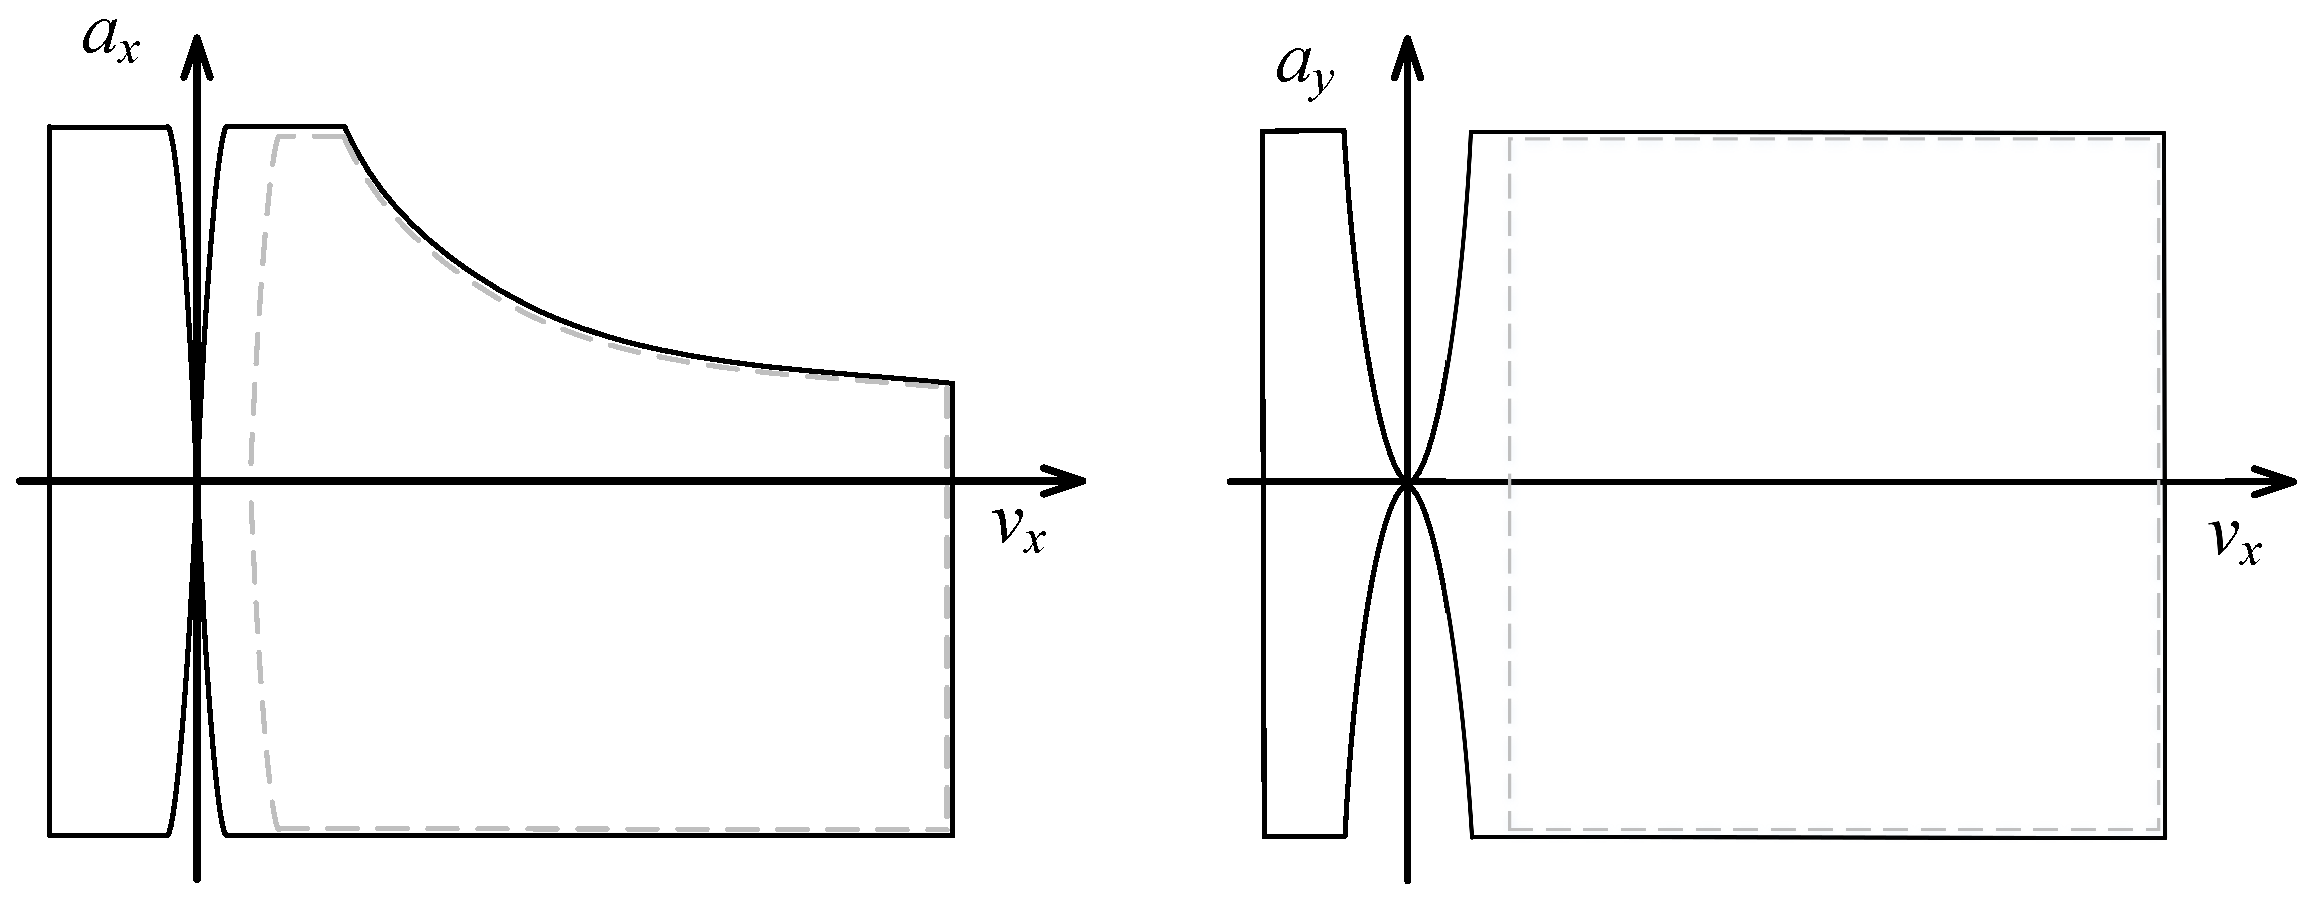
\includegraphics[width=10cm]{Bilder/01/betriebsbereich.eps}
    \caption{Quasistationäre Bewegungsgrenzen für Längs- und Querführung (manuelles Fahren, Ausweichassistent, ACC, Parkierassistent, Nothalteassistent)}
    \label{fig:bew_lims}
\end{figure}

Weiterhin müssen die Fahrerassistenzfunktionen bei variierenden Betriebsparametern bspw. einer von Fahrt zu Fahrt variierenden unbekannten Zusatzbeladung des Fahrzeugs, einer aufgrund eines Reifenwechsels unbekannten Bereifung, dem witterungsbedingt unsicheren Reifen-/Fahrbahnzustand, in einem unterschiedlich großen Fahrgeschwindigkeitsbereich gleichermaßen gut d.~h. robust gut funktionieren. Natürlich ist es möglich, verschiedene Einflußgrößen hierbei während der Fahrt zu schätzen bzw. zu beobachten und die Assistenzfunktion daran zu adaptieren.  
Abb.~\ref{fig:m_vert} zeigt hierzu exemplarisch den Einfluss einer zu berücksichtigenden Zusatzbeladung und deren Positionierung. Diese ergibt sich beispielsweise aus unterschiedlichen Derivaten, Motorisierungen, Sonderausstattungen innerhalb einer Produktlinie, der Zusatzbeladung selbst durch eine unterschiedliche Anzahl von Personen im Fahrzeug, Dachträger, Kofferraum, etc.. Ein Fehlermodell der Zusatzmasse wird erstellt welches ihren Einfluss auf die Fahrzeugparameter bspw. die Schwerpunktlage, Masse oder Träghheitsmomente beschreibt.  
%\begin{itemize}
%	\item Mathematische Beschreibung des Betriebsbereichs
%	\begin{itemize}
%		\item Fahrgeschwindigkeit
%		\item Reibwert
%		\item Beladung
%	\end{itemize} 
%\end{itemize} 
\begin{figure}[htp!]
\centering
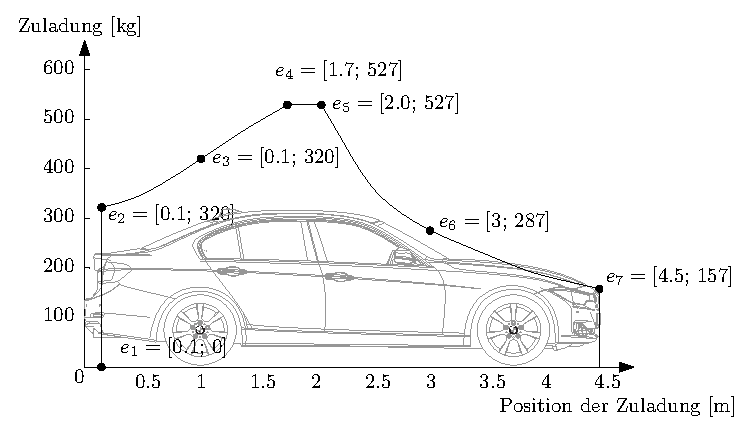
\includegraphics[width=8cm]{Bilder/01/massen_verteilung_f30.eps}
\label{fig:m_vert}
\end{figure}


%\subsubsection*{Grenzen}

%\begin{figure}[htp!]
%%  \centering
%    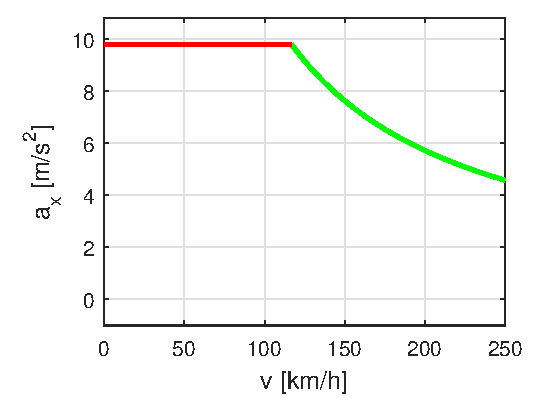
\includegraphics[scale=0.6]{Bilder/01/v_ax.eps}
%    \hspace{1cm}
%%   \caption{Grenzen L.}
%%   \label{fig:v_ax}
%%\end{figure}
%%\begin{figure}[htp!]
%%  \centering
%    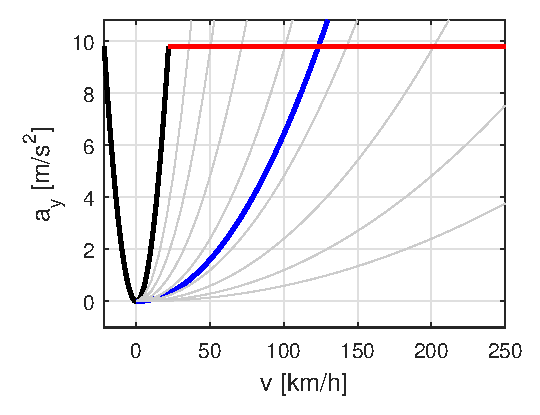
\includegraphics[scale=0.6]{Bilder/01/v_ay.eps}
%    \caption{Grenzen Längsdynamik}
%    \label{fig:v_ay}
%\end{figure}

\subsubsection*{Regelungsaufgabe}
Die modellbasierte Regelung MBC (\textit{Model Based Control}) 
entstand in den 1960er Jahren durch die Einführung des Zustandsraummodells durch Kalmann zusammen mit \textit{Optimal Control} 
und beinhaltet heute eine Vielzahl von Methoden für die Regelung von linearen und nichtlinearen Systemen. In einer Vielzahl von Anwendungen bspw. in der Flugregelung, der    
Robotik, der Vertikaldynamikregelung, der Fahrdynamikregelung, der Antriebsregelung, der Aktuatorregelung oder der Regelung im Zusammenhang mit Fahrerassistenzsystemen der Längs- und Querführung werden MBC Methoden heute sehr erfolgreich eingesetzt. Lineare Methoden beinhalten beispielsweise LMI, IMC, Polvorgabe, LQR, quasilineare Methoden wie die Popov-Methode oder das Zweiortskurvenverfahren sowie nichtlineare Methoden bspw. Lypunov-basierte Methoden oder Ein-/Ausgangslinearisierung.  Gemeinsame Grundlage für den erfolgreichen industriellen Einsatz dieser Methoden ist, dass ein einfaches physikalisches Modell der Regelstrecke existiert und Abweichungen von diesem Modell durch entsprechende mathematische Unsicherheitsmodelle beschrieben werden können. 
%Zunächst für den Entwurf in Form von parametrischen linearen/nichtlinearen zeitinvarianten Systemen in Zustands- oder Übertragungsform (\textit{linear parametric LTI system}), 
%numerisch linearer parametervariierender Systeme (\textit{LPV systems}), 
%additive oder multiplikative Unsicherheitsmodelle im Frequenzbereich (\textit{additive or multiplicative perturbation models}).
Für die Anwendung der integrierten Quer- und Längsführung haben sich aufgrund der Aufgabenstellung insbesondere lineare Verfahren mit einer ....  bewährt.
 
Die Regelungsaufgabe soll beschreiben welche Eigenschaften der geschlossene Regelkreis besitzen soll. Dies umfasst, dass der Regelkreis zunächst grundsätzlich stabil sein soll,
 d.~.h dass die Reaktion des geschlossenen Regelkreises auf externe Anregungen nicht zu einem instabilen Verhalten führt. Insbesondere sind hierbei Aspekte die durch numerische Diskretisierungsverfahren, Multirating, Quantisierungen, Totzeiten, Lose, Reibungseffekte, Sensorrauschen oder Strukturvariabilität im Stellprinzip(VDDS) zu beachten und bei Bedarf in der regelungstechnischen Synthese zu berücksichtigen.

Wesentliche Aufgabe ist es, ein gutes Führungs- und Störübertragungsverhalten zu realisieren. In unserem Fall bedeutet dies, dass Sollvorgaben für den Regelkreis durch eine Trajektorienplanung skalierbar steif und stationär genau eingeregelt werden können sollen. Störungen beispielsweise induziert durch Seitenwind, Reibwertsprünge sollen kompensiert werden.

Die Eigenschaften der Stabilität und des guten Führungs- und Störübertragungsverhaltens sollen robust sein gegenüber variierenden nicht mess-/schätz-/beobachtbaren Parametern und Fahrzustandsgrößen, gegenüber im Regelungsentwurf nicht berücksichtigten Modellierungsungenauigkeiten und beispielsweise nichtlinearen Effekten wie oben beschrieben.   


%Dies schließt auch die Vermeidung von nichtlinearer Grenzzyklen (Grenzschwingungen), häufig induziert durch nichtlineare  
  
%\begin{itemize}
%\item \emph{Stabilität} Zunächst muss Stabilität für das Gesamtsystem sichergestellt werden. Zum einen   
%Stabilität, asymptotische Stabilität nach Lyapunov
%absolute Stabilität Vermeidung nichtlinearer Grenzzyklen (Grenzschwingungen) in der Gegenwart von Nichtlinearitäten
%Vermeidung driver induced oscillations. Eine Überreaktion des Fahrers oder eine zeitlich ungünstig versetzte Reaktion des Fahrers kann zu ungewünschten Schwingungsphänomenen führen 
%
%\item \emph{Regelgüte} Führungs- und Störübertragungsverhalten im Sinne von schneller Einschwingzeit des Regelkreises
%
%\item \emph{Robustheit}
%\end{itemize}  
% 
% Diskretisierung, multirating, Totzeiten, Lose, Reibungsmodell, Sensorrauschen., strukturvariable Systeme (VDD)... 
%
% 
% Regelgüte
% 
% Robustheit der Eigenschaften Stabilität und Regelgüte bei variierenden Betriebsparametern
% Robustheit gegenüber nichtmodellierten Dynamiken
% 
Zusätzlich zum Fahrversuch bietet es sich an analytische Struktureignungsanalysen und simulativ gestützte Analysen mit komplexeren Fahrzeug-, Sensorik-, Aktuatorik- und Umgebungsmodellen durchzuführen.
 
 
 

%\subsubsection*{Kundenfunktionen}
%
%
%
%
%\begin{figure}[htp!]
%\centering
%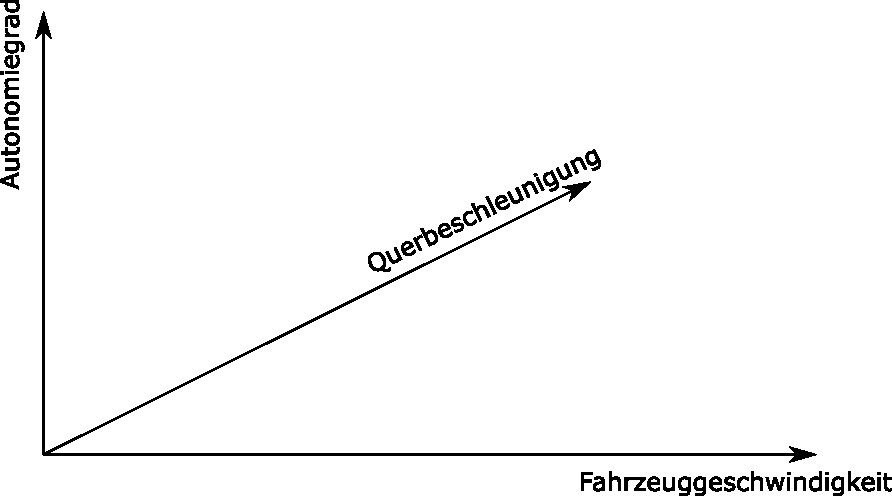
\includegraphics[width=12cm]{Bilder/01/KoordSys.pdf}
%\end{figure}
%
%
%
%%\begin{figure}[htp!]
%%\centering
%%\import{Bilder/01/}{Impedanzmodell_Lenkung.pdf_tex}
%%\caption{Grundstruktur des Störgrößenbeobachters mit Kompensation}
%%\label{fig:01_Lenkung}
%%\end{figure}
%
%%\begin{figure}[htp!]
%%\centering
%%\import{Bilder/01/}{Impedanzmodell_Lenkung_visio.pdf_tex}
%%\caption{Grundstruktur des Störgrößenbeobachters mit Kompensation}
%%\label{fig:01_Lenkung}
%%\end{figure}
%
%
%Ruckbegrenzung bei unterschiedlichen Anfangsgeschwindigkeiten
%
%
%
%
%\begin{figure}[htp!]
%  \centering
%    \includegraphics[scale=0.83]
%    {Bilder/01/Impedanzmodell_Lenkung.eps}
%    \caption{Kooperative Fahrzeugführung mit Regelstrecke für Querführung mittels Lenkung.}
%    \label{fig:Imp_Lenkung}
%\end{figure}
%
%\begin{figure}[htp!]
%  \centering
%    \includegraphics[scale=0.83]
%    {Bilder/01/Impedanzmodell_Quer.eps}
%    \caption{Kooperative Fahrzeugführung mit Regelstrecke für Querführung.}
%    \label{fig:Imp_Lenkung}
%\end{figure}
%
%\begin{figure}[htp!]
%  \centering
%    \includegraphics[scale=0.83]
%    {Bilder/01/Impedanzmodell_FF.eps}
%    \caption{Kooperative Fahrzeugführung mit Regelstrecke für Quer- und Längsführung.}
%    \label{fig:Imp_Lenkung}
%\end{figure}
%

%\section{Drei-Ebenen-Model des kooperativen und autonomen Fahrens}
\label{ch_3EM}
In Anlehnung an~\cite{Rasmussen1983} und~\cite{Donges1982} unterteilen wir die Fahraufgabe in die  \textit{Navigationsebene},  \textit{Bahnführungsebene} und  \textit{Fahrzeugführungsebene}.

In der \textit{Navigationsebene} werden neben der klassischen Aufgabe der Vorausplanung einer Fahrstrecke auch diskrete Entscheidungen innerhalb von Einzelfunktionen durchgeführt wie z.B. Parklücke links oder rechts wählen, Spur wechseln oder in der Spur verzögern, links oder rechts abbiegen, usw..

In der \textit{Bahnführungsebene} wird die durch die Navigationsebene vorgegeben Fahraufgabe umgesetzt.  Dabei muss das Fahrzeugumfeld berücksichtigt werden (prädizierte Objektbewegungen, Randbebauungen, etc.) und sichergestellt werden, dass die Fahrbarkeit anhand des Potenzials des Fahrzeugs gewährleistet ist. Die Bahnführungsebene ist fahrzeugparameterfrei und kennt nur die geometrischen Ausmaße der Fahrzeugkarosserie, um Kollisionsfreiheit prüfen zu können. Eine Trajektoriefolgeregelung längs und quer regelt geometrische Abweichungen von der Solltrajektorie bspw. aufgrund von Störungen aus und generiert als fahrzeugparameter- und geschwindigkeitsunabhängige Vorgaben der Quer- und Längsführung eine Sollkrümmung und eine Solllängsbeschleunigung für die unterlagerte \textit{Fahrzeugführungsebene}. Die Trajektoriefolgeregelung längs und quer erfolgt hierbei getrennt, +schlauer Halbsatz.

Das Potenzial, welche Trajektorien fahrbar sind, wird durch die unterlagerte \textit{Fahrzeugführungsebene} die die vollständige Information über die verbauten Sonderausstattungen, das Potenzial der Aktuatoren, der Fahrdynamik, Fahrzustandsbeobachter, Fahrzeugparameterschätzer, usw. besitzt und als abstrahierte Potenzialbeschreibung für eine mögliche Fahrzeugbewegung bereitstellt. In der \textit{Fahrzeugührungsebene} werden die fahrzeugparameterfreien Sollvorgaben Sollkrümmung und Längsbeschleunigung eingeregelt und die Aktuatoren angesteuert.
Hierbei ist es Aufgabe der kooperativen Fahrzeugführungsregelung quer und längs zum einen, ein möglichst gutes Führungsübertragungs- und Störübertragungsverhalten darzustellen,
und zum anderen die Fahrereingaben, im Sinne der beispielhaft für die Querführung in Abb.~\ref{fig:koopgrad} beschriebenen Kooperationsgrade, mit zu berücksichtigen. 

Abb.~\ref{fig:3EM} zeigt hierzu stark vereinfacht und schematisiert die angenommene Struktur eines Drei-Ebenen-Modells für manuelles, kooperatives und autonomes Fahren.
\begin{figure}[htp!]
  \centering
    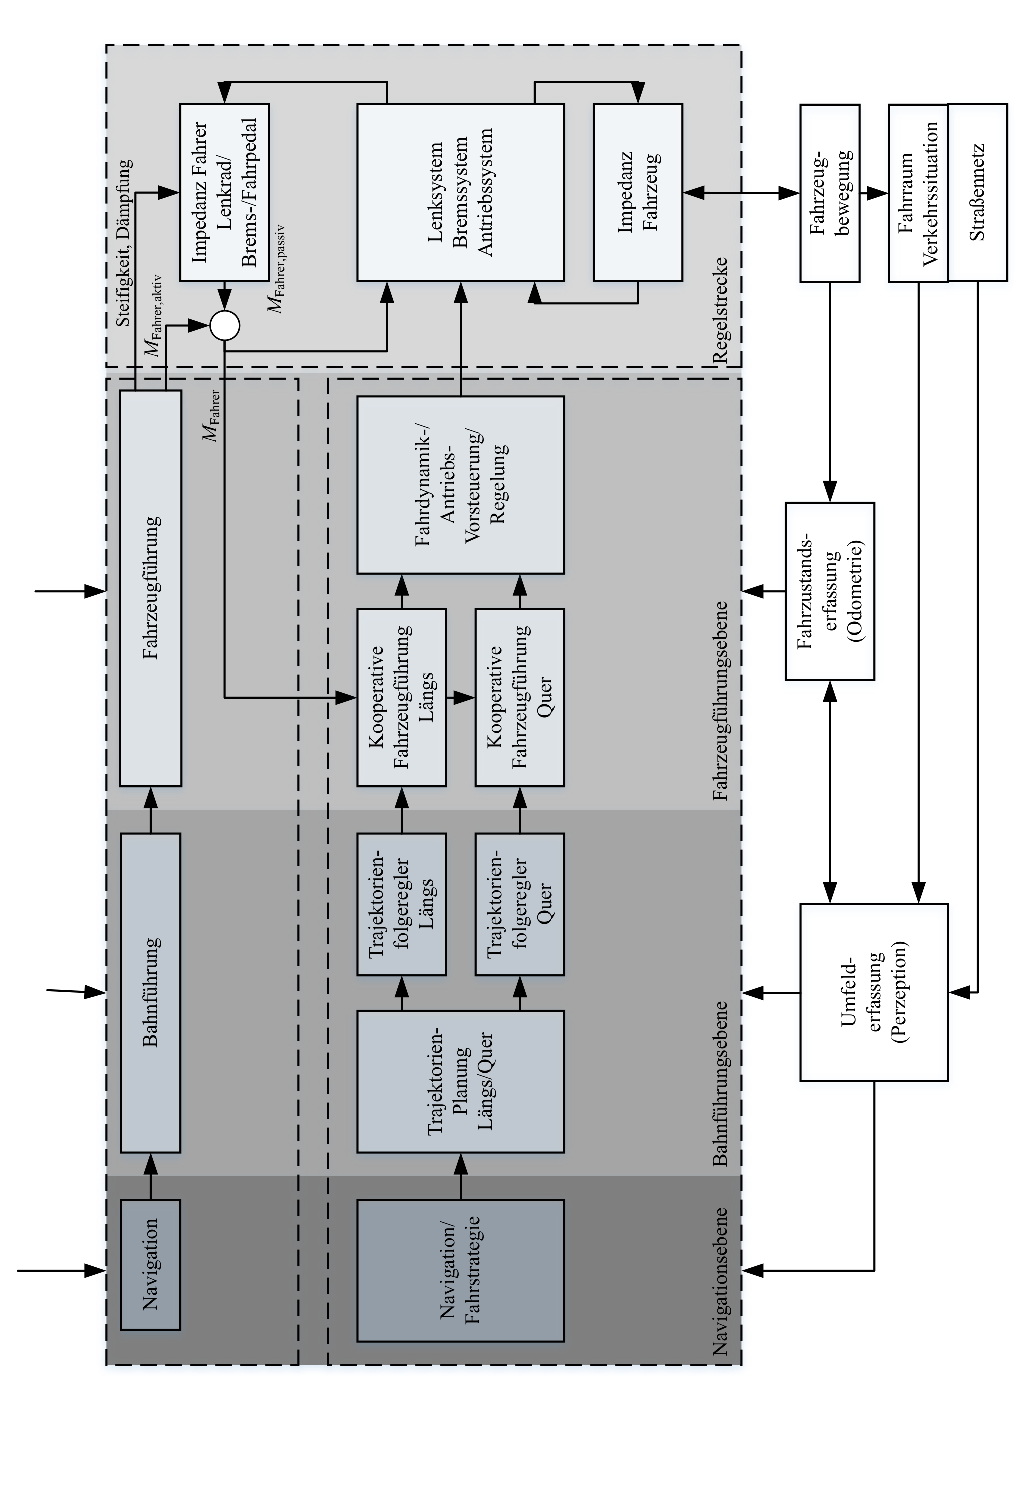
\includegraphics[scale=0.7]
    {Bilder/01/3EM.eps}
    \caption{Adaptiertes Drei-Ebenen-Modell für integrierte Quer- und Längsführung}
    \label{fig:3EM}
\end{figure}
Ausgangsseitig ist die Bahnführungsebene direkt an die Aktuatorregelungen der Fahrzeugführung angegliedert. Für die Querführung wird dabei als Schnittstelle eine umzusetzende Sollkrümmung $\kappa_\mathrm{d}$ übergeben.  Diese bietet den Vorteil der Unabhängigkeit von der Fahrzeuggeschwindigkeit. Damit sind Parkier- und Fahrfunktionen mit der gleichen Schnittstelle bedienbar. Des Weiteren ergibt sich eine Unabhängigkeit von verwendeten Aktuatorik auf der Bahnführungsebene: Innerhalb der Fahrzeugführungsebene können Vorderachs- und Hinterachslenkungen verwendet werden oder gegebenenfalls einseitige Bremseingriffe zur Erzeugung eines Giermoments, um die geforderte Sollkrümmung umzusetzen.\\ 
Bei der Längsführung wird eine Sollbeschleunigung $a_\mathrm{d}$ übergeben. Diese wird in ein Sollradmoment umgerechnet und je nach Betriebsbereich auf die beiden Aktuatoren Antrieb und Bremse verteilt. 

Im Rückkanal liefert die Fahrzeugführungsebene der Bahnführungsebene das ermittelte zur Verfügung stehende fahrdynamische Potenzial.  Dieses wird in abstrahierter Form bereitgestellt. Dazu werden geometrische Grenzen, Aktuatorgrenzen, physikalische Grenzen und Grenzen die aus der Funktionalen Sicherheit resultieren berücksichtigt.\\
Den Reifen eines Fahrzeugs kommt bei der Kraftübertragung eine entscheidende Rolle zu. Je nach Reibwert können diese nur eine bestimmte Kraft übertragen. In dynamisch unkritischen Situationen stellt sich der Kraftaufbau dabei linear zum anliegenden Schlupf ein. In hochdynamischen Situationen oder bei niedrigem Reibwert ist das Übertragungsverhalten allerdings gesättigt. Eine genaue Identifikation des Übertragungsverhaltens ist schwierig und immer noch Gegenstand der Forschung. Um nicht für jeden Reifen die Kennlinie einzeln identifizieren zu müssen, werden deshalb die idealisierten Zusammenhänge nach dem Kamm'schen Kreis verwendet. Dieser erlaubt eine Abschätzung der umsetzbaren Längs- und Querkräfte am Rad eines Fahrzeugs \cite{Risch2002}. Demnach kann die resultierende Kraft $\mathbf{F}_i$ eines Reifens nicht das Produkt aus dem Reibwert $\mu$
und der Normalkraft $F_{n,i}$ überschreiten:
\begin{equation}
|\mathbf{F}_i|= \sqrt{F_{q,i}^2 + F_{l,i} ^2} \leq \mu \, F_{n,i} \text{ mit } i \in [\text{vorne links}, \text{vorne rechts}, \text{hinten links}, \text{hinten rechts}]
\label{eq_kammscher_kreis}
\end{equation}
$F_{q,i}$ und $F_{l,i}$ stellen dabei am jeweiligen Rad die Quer- und Längskomponente der Kraft dar. Wird Bedingung (\ref{eq_kammscher_kreis}) eingehalten, so wird das Rad stets rollen und nicht in den Gleitzustand gelangen \cite{Mitschke2004}.
Da der Reibwert nicht direkt gemessen werden kann, müssen Schätzverfahren zur Ermittlung eingesetzt werden. Zur Reibwertschätzung stehen mittlerweile verschiedene Verfahren bereit, die auch bereits industrialisiert worden sind.\\
Da bei der Planung der zu fahrenden Trajektorien meist das Fahrzeug als Massenpunkt betrachtet wird, das heißt die einzelnen Räder nicht betrachtet werden, kann der Zusammenhang (\ref{eq_kammscher_kreis}) für das gesamte Fahrzeug auf Beschleunigungsebene betrachtet werden:
\begin{equation}
 \sqrt{a_x^2+a_y^2} \leq \mu \, g = a_{pot}
\end{equation}
Demnach ergibt sich die resultierende maximal fahrbare Beschleunigung $a_{pot}$ aus dem Reibwert und der Erdbeschleunigung $g$. $a_x$ beschreibt die Fahrzeuglängs- und $a_y$ die Fahrzeugquerbeschleunigung.
Für die Planung einer fahrbaren Trajektorie ist allerdings nicht der aktuelle Reibwert, sondern der zukünftige Reibwert relevant. Dies macht eine prädiktive Schätzung auf Basis von Umfeldsensorik nötig (siehe z.B. \cite{daniel2014reibwertschaetzung}).\\
Oft beschränkt nicht der Reibwert die fahrbare Trajektorie, sondern die unterlagerten Aktuatoren (gewöhnlich Antrieb, Bremse und Lenkung). Diese weisen konstruktionsbedingte Stellgrößenbegrenzungen auf oder aus Sicherheitsgründen werden ihre Stellraten- und/oder Stellgrößen auf für den Fahrer beherrschbare Werte begrenzt.\\
Bei der Querführung sind hierbei die Endanschläge der Lenkung zu berücksichtigen. Diese führen dazu, dass das Fahrzeug nicht beliebig kleine Radien fahren kann und stellen somit eine Sättigung der umsetzbaren Krümmung dar. Diese lässt sich durch die stationäre Verstärkung des Einspurmodells, das in Kapitel~\ref{ch_Modellierung} beschrieben wird, aus dem maximal möglichen Lenkwinkel $\delta_{max}$ berechnen:
\begin{equation}
\kappa_{max}=k_\kappa \, \tan \left(\delta_{max}\right) 
\end{equation}
Die maximal mögliche Krümmung kann mit 
\begin{equation}
a_{y,max} = \kappa_{max} v_x^2 
\end{equation}
und der aktuellen Fahrzeuggeschwindigkeit $v_x$ in eine maximal mögliche Querbeschleunigung $a_{y,max}$ umgerechnet werden.
\\ 
Auch der Antrieb kann nicht jedes beliebige Moment umsetzen. Über Schnittstellen zur Antriebsaktuatorik steht in modernen Fahrzeugarchitekturen allerdings serienmäßig das im aktuellen Gang maximal umsetzbare Radmoment $\tau_{mot,max}$ als Signal zur Verfügung. Dieses kann mittels der geschätzten Fahrzeugmasse $\tilde m$ und dem angenommenen dynamischen Rollradius $\tilde r$ in eine maximal mögliche Längsbeschleunigung $a_{x,mot,max}$ umgerechnet werden:
\begin{equation}
a_{x,ant,max} = \frac{1}{\tilde m \, \tilde r} \tau_{mot,max} 
\end{equation}
Des Weiteren muss bei niedrigem Reibwert die Antriebsart berücksichtigt werden, sodass das Beschleunigungspotenzial in Längsrichtung  bei einem rein front- oder heckgetriebenen Fahrzeug im Vergleich zu einem allradgetriebenen Fahrzeug bei ausreichendem Motormoment weiter beschränkt ist. Darüber hinaus können Fahrwiderstände, die die Fahrzeuglängsdynamik beeinflussen, berücksichtigt werden. So kann beispielsweise, wie in Kapitel~\ref{ch_Fahrzeugführungsebene} beschrieben wird, die aus den Fahrwiderständen resultierende Störbeschleunigung in Längsrichtung $\tilde z_{a_x}$ beobachtet werden und es ergibt sich als Potenzialgrenze in Längsrichtung
\begin{equation}
a_{x,pot} = a_{x,max} + \tilde z_{a_x}.
\end{equation}
Die maximale Verzögerung wird nicht begrenzt, da üblicherweise davon ausgegangen werden kann, dass die Bremsanlage die maximale Verzögerung erreichen kann.
	   \begin{figure}[thpb]
	      \centering
	  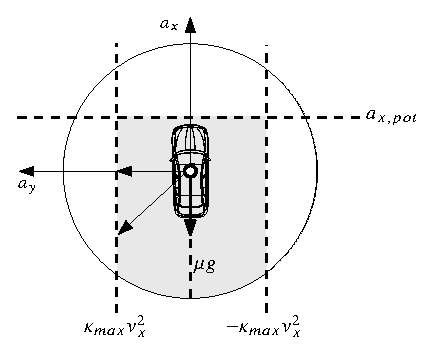
\includegraphics{Bilder/02/pot_vec.eps}
	 \begin{center}
	       \caption{Kamm'scher Kreis mit Begrenzungen.}
	      \label{abb_pot_vec}
	       \end{center}
	   \end{figure} 
%Auf die gleiche Weise wie bei $\kappa_{max}$ und $a_{x,max}$ 
Weiterhin können etwaige Stellratenbegrenzungen $\dot \kappa_{max}$ und $\dot a_{x,max}$ berücksichtigt werden.\\
Abb.~\ref{abb_pot_vec} veranschaulicht die Potenzialgrenzen, die sich aus den Aktuatorbegrenzungen und dem Kamm'schen Kreis ergeben. Die resultierende Beschleunigung der zu planenden Trajektorie darf folglich nur im grau markierten Bereich der Abbildung liegen. Dabei stellen die Grenzen Maximalwerte dar, die auf keinen Fall überschritten werden sollten. Gerade die Schätzung des Reibwerts ist meist nur möglich, wenn bereits großer Schlupf vorliegt. Von daher ist es sinnvoll, die Grenzen als absolutes Maximum zu betrachten und sich ihnen, falls möglich, konservativ zu nähern.\\
Die beschriebenen Größen werden im fahrdynamischen Potenzial zusammengefasst und der Bahnführungsebene zur Verfügung gestellt.\\
 NoNi: zwei geregelte Ebenen, eine gesteuerte! Wichtig Unterscheidung, auf deren Grundlage plausibel wird, dass wir im folgenden nur noch zwei Ebenen betrachten.
\FloatBarrier


\refFig{LongLatOverview} zeigt das Zusammenspiel aller an der integrierten Quer- und Längsregelung beteiligten Softwarekomponenten und Systeme.

%%%%%%%%%%%%%%%%%%%%%%%%%%%%%%%%%%%%%%%%%%%%%%%%%%%%%%%%%%%%%%%%%%
\begin{figure}[htp!]
\centering

\begingroup
\renewcommand*{\arraystretch}{0.75}
\import{Bilder/LongLatOverview/}{LongLat_Overview.pdf_tex}
\endgroup

\caption{Gesamtschau der kooperativen integrierten Längs-Quer-Regelung}
\label{fig:LongLatOverview}
\end{figure}
%%%%%%%%%%%%%%%%%%%%%%%%%%%%%%%%%%%%%%%%%%%%%%%%%%%%%%%%%%%%%%%%%%%


Die Trajektorienplanung (TP) erzeugt auf Grundlage der nicht dargestellten übergeordneten Navigations-/Fahrstrategieebene die Solltrajektorie 
$\begin{bmatrix}x & y & \theta & \kappa & v_x & a_x\end{bmatrix}^T_\mathrm{traj}$. Die nachgelagerten Trajektorienfolgeregler, TC\sus{lat} für die Querbewegung und TC\sus{long} für die Längsbewegung, errechnen aus der Solltrajektorie und der tatsächlichen Lage/Geschwindigkeit
$\begin{bmatrix}x & y & \theta & v_x\end{bmatrix}$ des Fahrzeugs die korrigierenden Stelleingriffe Sollkrümmung $\kappa_\mathrm{d}$ und Solllängsbeschleunigung $a_{x\mathrm{d}}$.

Diese werden durch die beiden Störgrößenbeobachter, DO\sus{$\kappa$} und DO\sus{$a_x$}, so ergänzt, dass beobachtete Störungen stationär kompensiert werden. Die adaptierte Sollkrümmung
$\kappaDPrime$ kann nun durch eine Stellgrößenverteilung (Control Allocation CA\sus{$\kappa$}) auf querdynamisch wirksame Aktuatoren verteilt werden. In den meisten Fällen wird das die Vorderachslenkung oder ein Lenksystem mit aufeinander abgestimmten Vorder- und Hinterachslenkwinkeln sein. Einseitige Bremseingriffe und eine direkte Ansteuerung der Hinterachslenkung sind hier auch denkbar. Der Anteil $\kappa_\delta$ der Sollkrümmung, welcher der Lenkung zugeordnete wurde, wird anschließend in einen Solllenkwinkel $\delta_\mathrm{d}$ umgerechnet. Die adaptierte Solllängsbeschleunigung $\aXDPrime$ wird vor der Verteilung auf Antrieb und Bremse (CA\sus{x}) in ein Sollmoment $\tau_{x\mathrm d}$ umgerechnet. Bei dieser Stellgrößenverteilung werden auch die vom Fahrer (Drv) über Bremspedal (BrkP) und Gaspedal (AccP) kommunizierten Wunschmomente berücksichtigt.

Die so berechneten Brems- und Antriebssollmomente $\tau_\mathrm{brk}$ und $\tau_\mathrm{mot}$ werden an die entsprechenden Aktuatorsteuergeräte übergeben und dort im Wesentlichen ohne Unterscheidung zwischen manuellem oder autonomen Fahren eingeregelt (Brk und Mot; die Blöcke repräsentieren jeweils Steuergerät und Aktuator). Für das Einstellen des Solllenkwinkels $\delta_\mathrm d$ wird im Gegensatz dazu ein zusätzlicher Regler, C\sus{$\delta$}, benötigt, der über die Anforderungen beim manuellen Fahren hinausgeht. 

Antrieb, Bremse und Lenkung (EPS) erzeugen über die Längs- und Querdynamik des Fahrzeugs (Vh\sus{lat} und Vh\sus{long}) die Fahrzeugbewegung, welche durch die tatsächliche Krümmung 
$\kappa$ und die tatsächliche Längsbeschleunigung $a_x$ beschrieben ist. Die dabei physikalisch auftretenden Rückwirkungen auf die Aktuatoren sind in Grau angedeutet.

Der äußere Regelkreis der Trajektorienfolgeregelung schließt sich über die Fahrzeugkinematik (Vh\sus{kin}), die $\kappa$ und $a_x$ zu $\begin{bmatrix}x & y & \theta & v_x\end{bmatrix}$ integriert.

\FloatBarrier


%\section{Fahrzeugmodelle}
\label{ch_Modellierung}
In diesem Abschnitt werden die Modelle der Fahrzeuglängs- und -querdynamik sowie die Modelle der  Aktuatoren beschrieben, die später Grundlage des Reglerentwurfs sind. Durch die verwendete Reglerstruktur, die robust gegen Modellfehler ist, konnte erreicht werden, dass sehr einfache lineare Modelle eingesetzt werden können.

%Die Regelung der Fahrzeugbewegung erfolgt Stand heute im Linearbereich der Fahrdynamik. Aufgabe der Trajektorienfolgeregelung und der unterlagerten Fahrzeugführungsregelung ist es bspw. einer bestimmten Trajektorienvorgabe zu folgen. Für die Längs- bzw. Quer-/Gierdynamik werden für den Funktionsentwurf separate quasilineare Modelle angenommen, die Vertikaldynamik wird vernachlässigt.

%%%%%%%%%%%%%%%%%%%%%%%%%%%%%%%%%%%%%%%%%%%%%%%%%%%%%%%%%%%%%%%%%
\subsection{Lenkung}\label{subS:SteeringModels}
Zwei Modelle, die das Verhalten des Vorderachslenksystems beschreiben, werden für die später formulierten Verfahren der Querregelung des Fahrzeugs benötigt.
Das Lenkungsmodell~1 beschreibt, wie sich der Vorderachslenkwinkel $\delta$ unter dem Einfluß der Stellgröße $\tau_{\delta\mathrm{d}}$ verhält, siehe \refFig{LongLatOverview}. 
Das Lenkungsmodell~2, beschreibt das Verhalten der Lenkung bei aktiver Lenkwinkelregelung mit dem Solllenkwinkel $\delta_\mathrm{d}$ als Eingang und dem Ist-Vorderachslenkwinkel 
$\delta$ als Ausgang, siehe \refFig{LongLatOverview}.

\subsubsection{Lenkungsmodell~1: Lenkmoment zu Lenkwinkelgeschwindigkeit}
Das Lenkungsmodell~1 ist ein stark vereinfachtes, lineares Modell der Vorderachslenkung mit dem Lenkmoment $\tau_{\delta\mathrm{d}}$ als Eingang und der Lenkwinkelgeschwindigkeit an der Vorderachse $\dot\delta$ als Ausgang.
$\tau_{\delta\mathrm{d}}$ ist dabei das Moment, welches zusätzlich zu den Momenten der Lenkunterstützungsfunktionen am Lenkaktuator angefordert wird. Als Übertragungsfunktion geschrieben hat das Modell die Form
\begin{equation}
G_{\tau\delta}(s)=\frac{1}{ms+b}\;\frac{1}{Ts+1}\label{eq:GL1}
\end{equation}
mit der Trägheit $m$, einem Dämpfungsbeiwert $b$ und einer Zeitkonstante $T$.
$G_{\tau\delta}$ wird als internes Modell für den in Abschnitt \ref{subS:DO_Delta} vorgestellten Störgrößenbeobachter im Lenkwinkelregler verwendet. 
Die Identifikation erfolgt mit aktiven Lenkunterstützungsfunkionen, die dadurch in ihrer Wirkung mit erfasst werden. Außerdem steht das Fahrzeug dabei auf einer Hebebühne, so dass die Rückkopplungen über die Reifenquerkräfte und Bohrmomente ausgeschaltet sind. \refFig{EpsIdent} zeigt beispielhaft den Vergleich des gemessenen und durch das Modell vorhergesagten Verlaufs der Lenkwinkelgeschwindigkeit. Die deutlichen Abweichungen lassen sich mit dem einfachen Modell nicht vermeiden. Der Störgrößenbeobachter ist aber, wie in Abschnitt \ref{subS:DO_Basic} ausgeführt wird, gegen diese Abweichungen robust und erzwingt im unteren Frequenzbereich das durch das Modell vorgegebene lineare Verhalten.


%\begin{figure}[htp!]
%\centering
%\import{Bilder/EpsIdent/}{EpsIdent.pdf_tex}
%\caption{Identifikation eines einfachen linearen Lenkungsmodells}\label{fig:EpsIdent}
%\label{fig:EpsIdent}
%\end{figure}


\subsubsection{Lenkungsmodell~2: Solllenkwinkel zu Istlenkwinkel}
Das Lenkungsmodell~2 fasst in einem einfachen linearen Modell das Verhalten der Lenkung inklusive Lenkwinkelregelung zusammen und beschreibt damit den dynamischen Zusammenhang zwischen Solllenkwinkel $\delta_\mathrm{d}$ und Istlenkwinkel $\delta$.
Dieses Modell wird zum einen als internes Modell für den in Abschnitt \ref{subS:DO_Kappa} vorgestellten Krümmungsstörgrößenbeobachter verwendet, der additive Störungen auf die Querdynamik kompensiert. Zum anderen wird das durch das Lenkungsmodell~2 beschriebene Verhalten bei der dynamischen Vorsteuerung im Trajektorienfolgeregler Quer berücksichtigt. Als Übertragungsfunktion geschrieben hat das Modell die Form

\begin{equation}
G_\delta^*(s)=\underbrace{\frac{k\omega_0^2}{s^2+2D\omega_0 s + \omega_0^2}}_{\displaystyle{G_\delta}}\;\mathrm{e}^{-T_\mathrm{D}s}\label{eq:GL2}
\end{equation}


Die Identifikation erfolgt im Fahrversuch anhand von Solllenkwinkelrampen $\delta_\mathrm{d}$ bei verschiedenen Fahrzeuggeschwindigkeiten, siehe \refFig{ident_zff}

\begin{figure}[htp!]
\begin{minipage}[t]{0.5\textwidth}
\centering
\scalebox{0.9}{\import{Bilder/EpsIdent/}{EpsIdent.pdf_tex}}
\parbox{0.9\textwidth}{\captionof{figure}{Identifikation Lenkungsverhalten Moment zu Lenkwinkelgeschwindigkeit, Vergleich Messung und Modell}\label{fig:EpsIdent}}
\end{minipage}
\begin{minipage}[t]{0.5\textwidth}
\centering
\setlength\figureheight{2.5cm} 
\setlength\figurewidth{5cm}
\scalebox{0.9}{%This file was created by matlab2tikz v0.5.0 running on MATLAB 7.11.1.
%Copyright (c) 2008--2014, Nico Schlömer <nico.schloemer@gmail.com>
%All rights reserved.
%Minimal pgfplots version: 1.3
%
%The latest updates can be retrieved from
%  http://www.mathworks.com/matlabcentral/fileexchange/22022-matlab2tikz
%where you can also make suggestions and rate matlab2tikz.
%
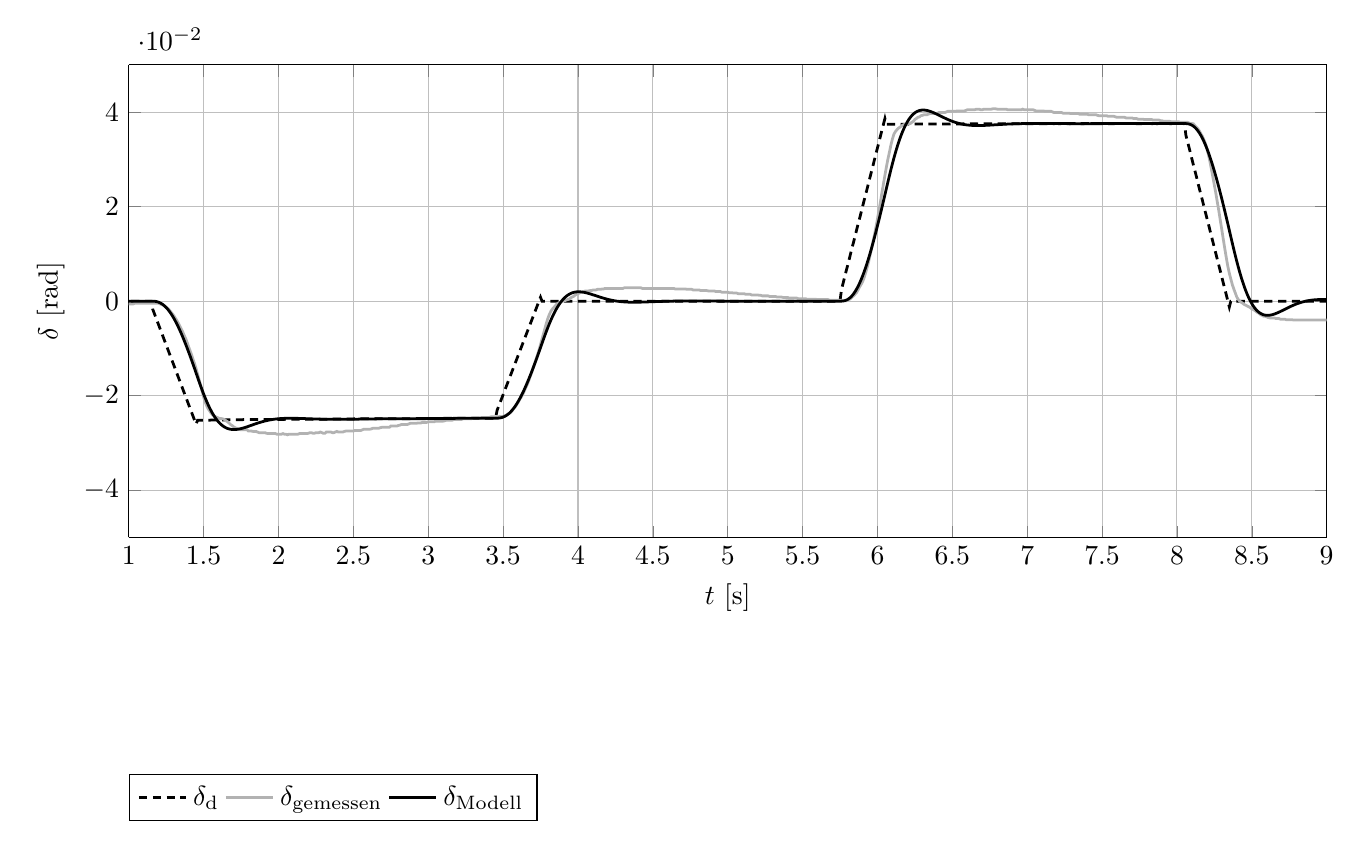
\begin{tikzpicture}

\begin{axis}[%
width=0.95092\figurewidth,
height=\figureheight,
at={(0\figurewidth,0\figureheight)},
scale only axis,
separate axis lines,
every outer x axis line/.append style={black},
every x tick label/.append style={font=\color{black}},
xmin=1,
xmax=9,
xlabel={$t$ [s]},
xmajorgrids,
every outer y axis line/.append style={black},
every y tick label/.append style={font=\color{black}},
ymin=-0.05,
ymax=0.05,
ylabel near ticks,
ylabel={$\delta\text{ [rad]}$},
ymajorgrids,
legend pos=south west,
legend style={legend cell align=left,align=left,draw=black,legend columns=3,at={(0.0,-0.6)}}
]
\addplot [color=black,densely dashed, line width=1]
  table[row sep=crcr]{%
0	1.38725944370566e-016\\
0.00999999999999801	1.38766813710271e-016\\
0.019999999999996	1.38766813710271e-016\\
0.0300000000000011	1.38748086341203e-016\\
0.0399999999999991	1.38748086341203e-016\\
0.0499999999999972	1.3878685133343e-016\\
0.0599999999999952	1.3878685133343e-016\\
0.0700000000000003	1.3882533839297e-016\\
0.0799999999999983	1.3882533839297e-016\\
0.0899999999999963	1.38864129854977e-016\\
0.100000000000001	1.38864129854977e-016\\
0.109999999999999	1.38806690433241e-016\\
0.119999999999997	1.38806690433241e-016\\
0.129999999999995	1.3873098686358e-016\\
0.140000000000001	1.3873098686358e-016\\
0.149999999999999	1.38733713250879e-016\\
0.159999999999997	1.38733713250879e-016\\
0.170000000000002	1.38590286750107e-016\\
0.18	1.38590286750107e-016\\
0.189999999999998	1.38622182834527e-016\\
0.199999999999996	1.38622182834527e-016\\
0.210000000000001	1.38653377469788e-016\\
0.219999999999999	1.38653377469788e-016\\
0.229999999999997	1.38684532400379e-016\\
0.240000000000002	1.38684532400379e-016\\
0.25	1.38628839984097e-016\\
0.259999999999998	1.38628839984097e-016\\
0.269999999999996	1.38604646605541e-016\\
0.280000000000001	1.38604646605541e-016\\
0.289999999999999	1.38485506127554e-016\\
0.299999999999997	1.38485506127554e-016\\
0.309999999999995	1.38498979245371e-016\\
0.32	1.38498979245371e-016\\
0.329999999999998	1.38486353160501e-016\\
0.339999999999996	1.38486353160501e-016\\
0.350000000000001	1.38461220104769e-016\\
0.359999999999999	1.38461220104769e-016\\
0.369999999999997	1.38460809823186e-016\\
0.379999999999995	1.38460809823186e-016\\
0.390000000000001	1.3848444733637e-016\\
0.399999999999999	1.3848444733637e-016\\
0.409999999999997	1.38395005951096e-016\\
0.420000000000002	1.38395005951096e-016\\
0.43	1.38339710581508e-016\\
0.439999999999998	1.38339710581508e-016\\
0.449999999999996	1.38361071693646e-016\\
0.460000000000001	1.38361071693646e-016\\
0.469999999999999	1.38283885816328e-016\\
0.479999999999997	1.38283885816328e-016\\
0.490000000000002	1.38303804325478e-016\\
0.5	1.38303804325478e-016\\
0.509999999999998	1.38323908123086e-016\\
0.519999999999996	1.38323908123086e-016\\
0.530000000000001	1.38348127971421e-016\\
0.539999999999999	1.38348127971421e-016\\
0.549999999999997	1.38259070397951e-016\\
0.559999999999995	1.38259070397951e-016\\
0.57	1.38215527610507e-016\\
0.579999999999998	1.38215527610507e-016\\
0.589999999999996	1.38189838689403e-016\\
0.600000000000001	1.38189838689403e-016\\
0.609999999999999	1.38121983409394e-016\\
0.619999999999997	1.38121983409394e-016\\
0.629999999999995	1.38188184328178e-016\\
0.640000000000001	1.38188184328178e-016\\
0.649999999999999	1.3815616912975e-016\\
0.659999999999997	1.3815616912975e-016\\
0.670000000000002	1.38174499452124e-016\\
0.68	1.38174499452124e-016\\
0.689999999999998	1.38191863627543e-016\\
0.699999999999996	1.38191863627543e-016\\
0.710000000000001	1.3809765768194e-016\\
0.719999999999999	1.3809765768194e-016\\
0.729999999999997	1.38115471843612e-016\\
0.740000000000002	1.38115471843612e-016\\
0.75	1.38113989535954e-016\\
0.759999999999998	1.38113989535954e-016\\
0.769999999999996	1.38117192379286e-016\\
0.780000000000001	1.38117192379286e-016\\
0.789999999999999	1.38122856912121e-016\\
0.799999999999997	1.38122856912121e-016\\
0.809999999999995	1.38140128443311e-016\\
0.82	1.38140128443311e-016\\
0.829999999999998	1.38100714941484e-016\\
0.839999999999996	1.38100714941484e-016\\
0.850000000000001	1.38078056810145e-016\\
0.859999999999999	1.38078056810145e-016\\
0.869999999999997	1.38062969035772e-016\\
0.879999999999995	1.38062969035772e-016\\
0.890000000000001	1.37972018873061e-016\\
0.899999999999999	1.37972018873061e-016\\
0.909999999999997	1.3794811666208e-016\\
0.920000000000002	1.3794811666208e-016\\
0.93	1.3797208504751e-016\\
0.939999999999998	1.3797208504751e-016\\
0.949999999999996	1.37986987533425e-016\\
0.960000000000001	1.37986987533425e-016\\
0.969999999999999	1.37957778131635e-016\\
0.979999999999997	1.37957778131635e-016\\
0.990000000000002	1.37986590486731e-016\\
1	1.37986590486731e-016\\
1.01	1.37861481073444e-016\\
1.02	1.37861481073444e-016\\
1.03	1.37879348174675e-016\\
1.04	1.37879348174675e-016\\
1.05	1.37898856402242e-016\\
1.06	1.37898856402242e-016\\
1.07	1.37811823766911e-016\\
1.08	1.37811823766911e-016\\
1.09	1.37824648375128e-016\\
1.1	1.37824648375128e-016\\
1.11	1.37841191987379e-016\\
1.12	1.37841191987379e-016\\
1.13	1.37751366790301e-016\\
1.14	1.37751366790301e-016\\
1.15	1.37690446592548e-016\\
1.16	-0.00168319279327989\\
1.17	-0.00252507580444217\\
1.18	-0.00336676905862987\\
1.19	-0.00420563062652946\\
1.2	-0.00504676206037402\\
1.21	-0.00588865019381046\\
1.22	-0.00672989897429943\\
1.23	-0.00757259223610163\\
1.24	-0.0084140133112669\\
1.25	-0.00925574079155922\\
1.26	-0.0100972075015306\\
1.27	-0.0109399175271392\\
1.28	-0.0117815006524324\\
1.29	-0.0126150036230683\\
1.3	-0.0134560689330101\\
1.31	-0.0142987323924899\\
1.32	-0.0151399169117212\\
1.33	-0.0159829054027796\\
1.34	-0.0168242193758488\\
1.35	-0.0176675785332918\\
1.36	-0.0185090247541666\\
1.37	-0.0193511005491018\\
1.38	-0.0201926100999117\\
1.39	-0.0210367348045111\\
1.4	-0.021878395229578\\
1.41	-0.0227165464311838\\
1.42	-0.0235581174492836\\
1.43	-0.024389885365963\\
1.44	-0.0252311620861292\\
1.45	-0.0260470118373632\\
1.46	-0.0252077691257\\
1.47	-0.0251978617161512\\
1.48	-0.0251978542655706\\
1.49	-0.0251942183822393\\
1.5	-0.025194214656949\\
1.51	-0.0251967515796423\\
1.52	-0.0251967534422874\\
1.53	-0.0251993183046579\\
1.54	-0.0251993220299482\\
1.55	-0.0251765977591276\\
1.56	-0.0251765828579664\\
1.57	-0.0251500494778156\\
1.58	-0.0251500308513641\\
1.59	-0.0251430813223124\\
1.6	-0.0251430775970221\\
1.61	-0.0251444280147552\\
1.62	-0.0251444280147552\\
1.63	-0.0251308344304562\\
1.64	-0.0251308251172304\\
1.65	-0.0251299701631069\\
1.66	-0.0251299701631069\\
1.67	-0.0251181665807962\\
1.68	-0.0251181554049253\\
1.69	-0.0251189190894365\\
1.7	-0.0251189190894365\\
1.71	-0.0251068063080311\\
1.72	-0.0251067988574505\\
1.73	-0.0250895489007235\\
1.74	-0.0250895339995623\\
1.75	-0.0250896029174328\\
1.76	-0.0250896029174328\\
1.77	-0.0250611752271652\\
1.78	-0.0250611528754234\\
1.79	-0.0250509288161993\\
1.8	-0.0250509213656187\\
1.81	-0.025050338357687\\
1.82	-0.025050338357687\\
1.83	-0.0250519383698702\\
1.84	-0.0250519402325153\\
1.85	-0.0250520445406437\\
1.86	-0.0250520445406437\\
1.87	-0.0250531155616045\\
1.88	-0.0250531155616045\\
1.89	-0.025029681622982\\
1.9	-0.0250296648591757\\
1.91	-0.0250318218022585\\
1.92	-0.0250318218022585\\
1.93	-0.0250322856009007\\
1.94	-0.0250322856009007\\
1.95	-0.0250334590673447\\
1.96	-0.0250334590673447\\
1.97	-0.0250340588390827\\
1.98	-0.0250340607017279\\
1.99	-0.0250277612358332\\
2	-0.0250277556478977\\
2.01	-0.0250296164304018\\
2.02	-0.0250296201556921\\
2.03	-0.0250267926603556\\
2.04	-0.0250267889350653\\
2.05	-0.0250097196549177\\
2.06	-0.0250097084790468\\
2.07	-0.0250140987336636\\
2.08	-0.0250141024589539\\
2.09	-0.0250153001397848\\
2.1	-0.0250153001397848\\
2.11	-0.0250184554606676\\
2.12	-0.0250184554606676\\
2.13	-0.0250216778367758\\
2.14	-0.0250216796994209\\
2.15	-0.0250125285238028\\
2.16	-0.0250125229358673\\
2.17	-0.0250104796141386\\
2.18	-0.0250104796141386\\
2.19	-0.0250127855688334\\
2.2	-0.0250127892941237\\
2.21	-0.0250064563006163\\
2.22	-0.025006452575326\\
2.23	-0.0250084735453129\\
2.24	-0.025008475407958\\
2.25	-0.0250115264207125\\
2.26	-0.0250115264207125\\
2.27	-0.0250150635838509\\
2.28	-0.025015065446496\\
2.29	-0.0250169206410646\\
2.3	-0.0250169206410646\\
2.31	-0.0249876119196415\\
2.32	-0.0249875895678997\\
2.33	-0.0249770991504192\\
2.34	-0.0249770916998386\\
2.35	-0.024980029091239\\
2.36	-0.0249800328165293\\
2.37	-0.024951284751296\\
2.38	-0.0249512642621994\\
2.39	-0.0249548051506281\\
2.4	-0.0249548070132732\\
2.41	-0.024951558560133\\
2.42	-0.0249515566974878\\
2.43	-0.0249455217272043\\
2.44	-0.024945518001914\\
2.45	-0.0249374303966761\\
2.46	-0.0249374248087406\\
2.47	-0.0249229241162539\\
2.48	-0.024922912940383\\
2.49	-0.024925708770752\\
2.5	-0.024925708770752\\
2.51	-0.0249110255390406\\
2.52	-0.0249110125005245\\
2.53	-0.0249148532748222\\
2.54	-0.0249148570001125\\
2.55	-0.0249130353331566\\
2.56	-0.0249130353331566\\
2.57	-0.0249126181006432\\
2.58	-0.0249126181006432\\
2.59	-0.024902019649744\\
2.6	-0.0249020121991634\\
2.61	-0.0249045789241791\\
2.62	-0.0249045789241791\\
2.63	-0.024896802380681\\
2.64	-0.0248967949301004\\
2.65	-0.0248977337032557\\
2.66	-0.0248977337032557\\
2.67	-0.0249009467661381\\
2.68	-0.0249009504914284\\
2.69	-0.0249037742614746\\
2.7	-0.0249037761241198\\
2.71	-0.0249055977910757\\
2.72	-0.0249055977910757\\
2.73	-0.0249058324843645\\
2.74	-0.0249058324843645\\
2.75	-0.0248987805098295\\
2.76	-0.0248987749218941\\
2.77	-0.0248882342129946\\
2.78	-0.024888226762414\\
2.79	-0.024883272126317\\
2.8	-0.0248832684010267\\
2.81	-0.0248767901211977\\
2.82	-0.0248767863959074\\
2.83	-0.0248700156807899\\
2.84	-0.0248700119554996\\
2.85	-0.0248718652874231\\
2.86	-0.0248718671500683\\
2.87	-0.024872774258256\\
2.88	-0.024872774258256\\
2.89	-0.0248555485159159\\
2.9	-0.0248555392026901\\
2.91	-0.0248473901301622\\
2.92	-0.0248473845422268\\
2.93	-0.02484923414886\\
2.94	-0.0248492360115051\\
2.95	-0.0248295236378908\\
2.96	-0.0248295087367296\\
2.97	-0.0248205754905939\\
2.98	-0.0248205661773682\\
2.99	-0.0248233787715435\\
3	-0.0248233787715435\\
3.01	-0.0248213857412338\\
3.02	-0.0248213838785887\\
3.03	-0.024823134765029\\
3.04	-0.024823134765029\\
3.05	-0.0248174350708723\\
3.06	-0.024817431345582\\
3.07	-0.024819815531373\\
3.08	-0.0248198192566633\\
3.09	-0.0247982516884804\\
3.1	-0.0247982386499643\\
3.11	-0.0247992184013128\\
3.12	-0.0247992184013128\\
3.13	-0.0248019769787788\\
3.14	-0.024801978841424\\
3.15	-0.0248056501150131\\
3.16	-0.0248056538403034\\
3.17	-0.0247917771339417\\
3.18	-0.0247917715460062\\
3.19	-0.0247949026525021\\
3.2	-0.0247949026525021\\
3.21	-0.0247856490314007\\
3.22	-0.0247856415808201\\
3.23	-0.0247888527810574\\
3.24	-0.0247888546437025\\
3.25	-0.0247898008674383\\
3.26	-0.0247898008674383\\
3.27	-0.0247849002480507\\
3.28	-0.0247848983854055\\
3.29	-0.0247823316603899\\
3.3	-0.0247823316603899\\
3.31	-0.0247864294797182\\
3.32	-0.0247864313423634\\
3.33	-0.0247864425182343\\
3.34	-0.0247864425182343\\
3.35	-0.024773932993412\\
3.36	-0.0247739236801863\\
3.37	-0.0247776992619038\\
3.38	-0.0247777011245489\\
3.39	-0.02477559261024\\
3.4	-0.0247755888849497\\
3.41	-0.0247652102261782\\
3.42	-0.0247652065008879\\
3.43	-0.0247664321213961\\
3.44	-0.0247664358466864\\
3.45	-0.0247680302709341\\
3.46	-0.0231174398213625\\
3.47	-0.0222903974354267\\
3.48	-0.0214646514505148\\
3.49	-0.0206431429833174\\
3.5	-0.0198172684758902\\
3.51	-0.018988186493516\\
3.52	-0.0181624833494425\\
3.53	-0.0173335503786802\\
3.54	-0.016508037224412\\
3.55	-0.0156750120222569\\
3.56	-0.0148499216884375\\
3.57	-0.0140272444114089\\
3.58	-0.0132020451128483\\
3.59	-0.0123767796903849\\
3.6	-0.0115516064688563\\
3.61	-0.0107263987883925\\
3.62	-0.00990125071257353\\
3.63	-0.00907474663108587\\
3.64	-0.00824973825365305\\
3.65	-0.00742613431066275\\
3.66	-0.00660098856315017\\
3.67	-0.00577646680176258\\
3.68	-0.00495124468579888\\
3.69	-0.0041267448104918\\
3.7	-0.00330138951539993\\
3.71	-0.0024752167519182\\
3.72	-0.00165014201775193\\
3.73	-0.00082456151721999\\
3.74	0\\
3.75	0.000824572693090886\\
3.76	0\\
3.77	1.34931276471536e-016\\
3.78	1.34931276471536e-016\\
3.79	1.34955827192117e-016\\
3.8	1.34955827192117e-016\\
3.81	1.34983818984046e-016\\
3.82	1.34983818984046e-016\\
3.83	1.34974673675193e-016\\
3.84	1.34974673675193e-016\\
3.85	1.34961677013409e-016\\
3.86	1.34961677013409e-016\\
3.87	1.34878442791451e-016\\
3.88	1.34878442791451e-016\\
3.89	1.34871348890518e-016\\
3.9	1.34871348890518e-016\\
3.91	1.34846771700158e-016\\
3.92	1.34846771700158e-016\\
3.93	1.34846771700158e-016\\
3.94	1.34846771700158e-016\\
3.95	1.34867947523839e-016\\
3.96	1.34867947523839e-016\\
3.97	1.34889890971129e-016\\
3.98	1.34889890971129e-016\\
3.99	1.34915275489767e-016\\
4	1.34915275489767e-016\\
4.01	1.34893623210053e-016\\
4.02	1.34893623210053e-016\\
4.03	1.34824629729521e-016\\
4.04	1.34824629729521e-016\\
4.05	1.34847909900681e-016\\
4.06	1.34847909900681e-016\\
4.07	1.34809197848013e-016\\
4.08	1.34809197848013e-016\\
4.09	1.34856883155966e-016\\
4.1	1.34856883155966e-016\\
4.11	1.34817138781894e-016\\
4.12	1.34817138781894e-016\\
4.13	1.34882042681477e-016\\
4.14	1.34882042681477e-016\\
4.15	1.34825410588019e-016\\
4.16	1.34825410588019e-016\\
4.17	1.34796955574947e-016\\
4.18	1.34796955574947e-016\\
4.19	1.34813340368521e-016\\
4.2	1.34813340368521e-016\\
4.21	1.34815841762693e-016\\
4.22	1.34815841762693e-016\\
4.23	1.34874088512707e-016\\
4.24	1.34874088512707e-016\\
4.25	1.34820235746107e-016\\
4.26	1.34820235746107e-016\\
4.27	1.34855467022757e-016\\
4.28	1.34855467022757e-016\\
4.29	1.34832054502699e-016\\
4.3	1.34832054502699e-016\\
4.31	1.3487122977651e-016\\
4.32	1.3487122977651e-016\\
4.33	1.34827938451971e-016\\
4.34	1.34827938451971e-016\\
4.35	1.34872434151482e-016\\
4.36	1.34872434151482e-016\\
4.37	1.34845673204304e-016\\
4.38	1.34845673204304e-016\\
4.39	1.348572272631e-016\\
4.4	1.348572272631e-016\\
4.41	1.34906222825143e-016\\
4.42	1.34906222825143e-016\\
4.43	1.34905336087527e-016\\
4.44	1.34905336087527e-016\\
4.45	1.34961107913147e-016\\
4.46	1.34961107913147e-016\\
4.47	1.34905931657568e-016\\
4.48	1.34905931657568e-016\\
4.49	1.34925241361787e-016\\
4.5	1.34925241361787e-016\\
4.51	1.34920159164103e-016\\
4.52	1.34920159164103e-016\\
4.53	1.34975454533691e-016\\
4.54	1.34975454533691e-016\\
4.55	1.34996590652703e-016\\
4.56	1.34996590652703e-016\\
4.57	1.34981291120094e-016\\
4.58	1.34981291120094e-016\\
4.59	1.34992593715984e-016\\
4.6	1.34992593715984e-016\\
4.61	1.35049040520984e-016\\
4.62	1.35049040520984e-016\\
4.63	1.35017091497005e-016\\
4.64	1.35017091497005e-016\\
4.65	1.35021313426851e-016\\
4.66	1.35021313426851e-016\\
4.67	1.35045109758713e-016\\
4.68	1.35045109758713e-016\\
4.69	1.35021551654868e-016\\
4.7	1.35021551654868e-016\\
4.71	1.35047743501784e-016\\
4.72	1.35047743501784e-016\\
4.73	1.3506062104956e-016\\
4.74	1.3506062104956e-016\\
4.75	1.35122202991803e-016\\
4.76	1.35122202991803e-016\\
4.77	1.35134286446191e-016\\
4.78	1.35134286446191e-016\\
4.79	1.35060660754229e-016\\
4.8	1.35060660754229e-016\\
4.81	1.3508387475094e-016\\
4.82	1.3508387475094e-016\\
4.83	1.35079996928228e-016\\
4.84	1.35079996928228e-016\\
4.85	1.35165428141893e-016\\
4.86	1.35165428141893e-016\\
4.87	1.35106294654263e-016\\
4.88	1.35106294654263e-016\\
4.89	1.35149493334573e-016\\
4.9	1.35149493334573e-016\\
4.91	1.35126967552132e-016\\
4.92	1.35126967552132e-016\\
4.93	1.35192572900874e-016\\
4.94	1.35192572900874e-016\\
4.95	1.35129918932557e-016\\
4.96	1.35129918932557e-016\\
4.97	1.35142439138309e-016\\
4.98	1.35142439138309e-016\\
4.99	1.35177035140248e-016\\
5	1.35177035140248e-016\\
5.01	1.35153371157284e-016\\
5.02	1.35153371157284e-016\\
5.03	1.35234527501543e-016\\
5.04	1.35234527501543e-016\\
5.05	1.35193869920075e-016\\
5.06	1.35193869920075e-016\\
5.07	1.35254790117828e-016\\
5.08	1.35254790117828e-016\\
5.09	1.35242772837889e-016\\
5.1	1.35242772837889e-016\\
5.11	1.35229101196725e-016\\
5.12	1.35229101196725e-016\\
5.13	1.3523141730244e-016\\
5.14	1.3523141730244e-016\\
5.15	1.35256338599935e-016\\
5.16	1.35256338599935e-016\\
5.17	1.35279407012858e-016\\
5.18	1.35279407012858e-016\\
5.19	1.35243831629073e-016\\
5.2	1.35243831629073e-016\\
5.21	1.35332320102281e-016\\
5.22	1.35332320102281e-016\\
5.23	1.35336303804112e-016\\
5.24	1.35336303804112e-016\\
5.25	1.35301496043935e-016\\
5.26	1.35301496043935e-016\\
5.27	1.35317073509231e-016\\
5.28	1.35317073509231e-016\\
5.29	1.35338646379606e-016\\
5.3	1.35338646379606e-016\\
5.31	1.35418611583783e-016\\
5.32	1.35418611583783e-016\\
5.33	1.35410405952106e-016\\
5.34	1.35410405952106e-016\\
5.35	1.35421708547996e-016\\
5.36	1.35421708547996e-016\\
5.37	1.35433937586172e-016\\
5.38	1.35433937586172e-016\\
5.39	1.35481106733423e-016\\
5.4	1.35481106733423e-016\\
5.41	1.35469102688373e-016\\
5.42	1.35469102688373e-016\\
5.43	1.35464973402755e-016\\
5.44	1.35464973402755e-016\\
5.45	1.35504638367489e-016\\
5.46	1.35504638367489e-016\\
5.47	1.35519779081421e-016\\
5.48	1.35519779081421e-016\\
5.49	1.35578065536104e-016\\
5.5	1.35578065536104e-016\\
5.51	1.35590612211635e-016\\
5.52	1.35590612211635e-016\\
5.53	1.35614461483056e-016\\
5.54	1.35614461483056e-016\\
5.55	1.35634075589741e-016\\
5.56	1.35634075589741e-016\\
5.57	1.35645060548276e-016\\
5.58	1.35645060548276e-016\\
5.59	1.35637979882232e-016\\
5.6	1.35637979882232e-016\\
5.61	1.3564543112519e-016\\
5.62	1.3564543112519e-016\\
5.63	1.35684738747898e-016\\
5.64	1.35684738747898e-016\\
5.65	1.35673184689102e-016\\
5.66	1.35673184689102e-016\\
5.67	1.3578032112204e-016\\
5.68	1.3578032112204e-016\\
5.69	1.35787600311431e-016\\
5.7	1.35787600311431e-016\\
5.71	1.35736381287901e-016\\
5.72	1.35736381287901e-016\\
5.73	1.35783616609601e-016\\
5.74	1.35783616609601e-016\\
5.75	1.35782796046433e-016\\
5.76	0.00245660915970802\\
5.77	0.00368707999587059\\
5.78	0.00498254224658012\\
5.79	0.00624298397451639\\
5.8	0.0074384668841958\\
5.81	0.00867043156176806\\
5.82	0.00996604189276695\\
5.83	0.0112340282648802\\
5.84	0.0124306194484234\\
5.85	0.0136608853936195\\
5.86	0.0149572547525167\\
5.87	0.0162162110209465\\
5.88	0.0174130797386169\\
5.89	0.0186487417668104\\
5.9	0.019941434264183\\
5.91	0.0211933236569166\\
5.92	0.0224109590053558\\
5.93	0.0236469935625792\\
5.94	0.0249325875192881\\
5.95	0.0261870045214891\\
5.96	0.02741121314466\\
5.97	0.0286500584334135\\
5.98	0.0299318917095661\\
5.99	0.0311878342181444\\
6	0.0324172414839268\\
6.01	0.0336417630314827\\
6.02	0.0349307283759117\\
6.03	0.0361873805522919\\
6.04	0.0374184548854828\\
6.05	0.0386564619839191\\
6.06	0.0374276675283909\\
6.07	0.0374386310577393\\
6.08	0.0374386496841908\\
6.09	0.0374365150928497\\
6.1	0.0374365076422691\\
6.11	0.037445455789566\\
6.12	0.0374454706907272\\
6.13	0.0374514497816563\\
6.14	0.0374514609575272\\
6.15	0.0374540984630585\\
6.16	0.0374540984630585\\
6.17	0.0374520644545555\\
6.18	0.0374520570039749\\
6.19	0.0374608859419823\\
6.2	0.0374608971178532\\
6.21	0.0374642610549927\\
6.22	0.037464264780283\\
6.23	0.0374734066426754\\
6.24	0.0374734252691269\\
6.25	0.0374756082892418\\
6.26	0.0374756082892418\\
6.27	0.0374830365180969\\
6.28	0.0374830476939678\\
6.29	0.0374876484274864\\
6.3	0.0374876596033573\\
6.31	0.0374681614339352\\
6.32	0.0374681353569031\\
6.33	0.0374891124665737\\
6.34	0.0374891459941864\\
6.35	0.0374921075999737\\
6.36	0.0374921150505543\\
6.37	0.0374836586415768\\
6.38	0.0374836400151253\\
6.39	0.0374913327395916\\
6.4	0.0374913439154625\\
6.41	0.0374819897115231\\
6.42	0.0374819785356522\\
6.43	0.03749905154109\\
6.44	0.0374990850687027\\
6.45	0.0375012680888176\\
6.46	0.0375012755393982\\
6.47	0.037485770881176\\
6.48	0.0374857448041439\\
6.49	0.0375045388936996\\
6.5	0.037504568696022\\
6.51	0.0375087931752205\\
6.52	0.0375088006258011\\
6.53	0.0375001356005669\\
6.54	0.0375001206994057\\
6.55	0.0375151969492435\\
6.56	0.0375152193009853\\
6.57	0.0375194996595383\\
6.58	0.0375195071101189\\
6.59	0.0375288128852844\\
6.6	0.0375288240611553\\
6.61	0.0375287719070911\\
6.62	0.0375287719070911\\
6.63	0.0375222377479076\\
6.64	0.0375222228467464\\
6.65	0.0375341475009918\\
6.66	0.0375341661274433\\
6.67	0.0375162363052368\\
6.68	0.0375162065029144\\
6.69	0.0375388376414776\\
6.7	0.0375388786196709\\
6.71	0.0375444293022156\\
6.72	0.0375444442033768\\
6.73	0.0375351272523403\\
6.74	0.0375351123511791\\
6.75	0.0375455133616924\\
6.76	0.0375455319881439\\
6.77	0.0375355891883373\\
6.78	0.0375355705618858\\
6.79	0.0375406034290791\\
6.8	0.0375406183302403\\
6.81	0.0375522002577782\\
6.82	0.0375522188842297\\
6.83	0.0375510938465595\\
6.84	0.0375510901212692\\
6.85	0.0375560633838177\\
6.86	0.0375560708343983\\
6.87	0.0375610999763012\\
6.88	0.0375611111521721\\
6.89	0.0375638641417027\\
6.9	0.037563867866993\\
6.91	0.0375544466078281\\
6.92	0.0375544279813766\\
6.93	0.0375544205307961\\
6.94	0.0375544205307961\\
6.95	0.0375536791980267\\
6.96	0.0375536791980267\\
6.97	0.0375510901212692\\
6.98	0.0375510901212692\\
6.99	0.0375646352767944\\
7	0.0375646576285362\\
7.01	0.0375605151057243\\
7.02	0.0375605076551437\\
7.03	0.0375755690038204\\
7.04	0.0375755950808525\\
7.05	0.0375698879361153\\
7.06	0.0375698804855347\\
7.07	0.037564430385828\\
7.08	0.0375644229352474\\
7.09	0.0375745035707951\\
7.1	0.0375745184719563\\
7.11	0.0375583320856094\\
7.12	0.0375583060085773\\
7.13	0.0375744178891182\\
7.14	0.0375744439661503\\
7.15	0.0375727452337742\\
7.16	0.0375727415084839\\
7.17	0.0375716388225555\\
7.18	0.0375716350972652\\
7.19	0.0375917591154575\\
7.2	0.0375917926430702\\
7.21	0.0375705398619175\\
7.22	0.0375705063343048\\
7.23	0.0375710912048817\\
7.24	0.0375710912048817\\
7.25	0.0375733263790607\\
7.26	0.037573330104351\\
7.27	0.0375569649040699\\
7.28	0.0375569388270378\\
7.29	0.0375782400369644\\
7.3	0.0375782772898674\\
7.31	0.037579357624054\\
7.32	0.037579357624054\\
7.33	0.0375860333442688\\
7.34	0.0375860407948494\\
7.35	0.0375756174325943\\
7.36	0.0375756025314331\\
7.37	0.0375733599066734\\
7.38	0.0375733561813831\\
7.39	0.0375844798982143\\
7.4	0.0375844985246658\\
7.41	0.0375800095498562\\
7.42	0.0375800020992756\\
7.43	0.0375729911029339\\
7.44	0.0375729762017727\\
7.45	0.037580031901598\\
7.46	0.0375800393521786\\
7.47	0.0375956557691097\\
7.48	0.0375956781208515\\
7.49	0.037584912031889\\
7.5	0.0375848971307278\\
7.51	0.0375822596251965\\
7.52	0.0375822558999062\\
7.53	0.0375766828656197\\
7.54	0.0375766716897488\\
7.55	0.0375693440437317\\
7.56	0.0375693365931511\\
7.57	0.0375726781785488\\
7.58	0.0375726819038391\\
7.59	0.0375834479928017\\
7.6	0.0375834666192532\\
7.61	0.0375911332666874\\
7.62	0.0375911444425583\\
7.63	0.0376010574400425\\
7.64	0.0376010723412037\\
7.65	0.0375848934054375\\
7.66	0.0375848673284054\\
7.67	0.0375767350196838\\
7.68	0.0375767201185226\\
7.69	0.0376012027263641\\
7.7	0.0376012399792671\\
7.71	0.037571519613266\\
7.72	0.0375714711844921\\
7.73	0.0375725999474525\\
7.74	0.0375726036727428\\
7.75	0.0375715345144272\\
7.76	0.0375715270638466\\
7.77	0.0375803560018539\\
7.78	0.0375803746283054\\
7.79	0.0375834442675114\\
7.8	0.0375834479928017\\
7.81	0.0375785529613495\\
7.82	0.0375785455107689\\
7.83	0.0375756286084652\\
7.84	0.0375756211578846\\
7.85	0.0375778637826443\\
7.86	0.0375778675079346\\
7.87	0.0375566110014915\\
7.88	0.0375565774738789\\
7.89	0.0375878624618053\\
7.9	0.0375879108905792\\
7.91	0.0375856570899487\\
7.92	0.0375856533646584\\
7.93	0.0375791266560555\\
7.94	0.0375791117548943\\
7.95	0.037575613707304\\
7.96	0.0375756099820137\\
7.97	0.0375739894807339\\
7.98	0.0375739894807339\\
7.99	0.037573903799057\\
8	0.037573903799057\\
8.01	0.0375812388956547\\
8.02	0.0375812537968159\\
8.03	0.0375896021723747\\
8.04	0.0375896133482456\\
8.05	0.037572342902422\\
8.06	0.0351007953286171\\
8.07	0.0338788330554962\\
8.08	0.0326407216489315\\
8.09	0.0313958637416363\\
8.1	0.0300913080573082\\
8.11	0.0288157314062119\\
8.12	0.0276117268949747\\
8.13	0.0263731963932514\\
8.14	0.0250691846013069\\
8.15	0.0238000005483627\\
8.16	0.0225854441523552\\
8.17	0.0213533919304609\\
8.18	0.0200679954141378\\
8.19	0.0188131742179394\\
8.2	0.0175791643559933\\
8.21	0.0163464229553938\\
8.22	0.0150637309998274\\
8.23	0.013805728405714\\
8.24	0.012564716860652\\
8.25	0.0113221034407616\\
8.26	0.0100487535819411\\
8.27	0.0087902033701539\\
8.28	0.00754886912181973\\
8.29	0.00631502782925963\\
8.3	0.00503526069223881\\
8.31	0.00377762690186501\\
8.32	0.00253930292092264\\
8.33	0.00130341411568224\\
8.34	2.39882501773536e-005\\
8.35	-0.00123366096522659\\
8.36	0\\
8.37	1.36649429865482e-016\\
8.38	1.36649429865482e-016\\
8.39	1.36703362041421e-016\\
8.4	1.36703362041421e-016\\
8.41	1.36625130607808e-016\\
8.42	1.36625130607808e-016\\
8.43	1.366575825576e-016\\
8.44	1.366575825576e-016\\
8.45	1.36639331644564e-016\\
8.46	1.36639331644564e-016\\
8.47	1.36637518464662e-016\\
8.48	1.36637518464662e-016\\
8.49	1.36752979643284e-016\\
8.5	1.36752979643284e-016\\
8.51	1.36699537158268e-016\\
8.52	1.36699537158268e-016\\
8.53	1.36664332351398e-016\\
8.54	1.36664332351398e-016\\
8.55	1.36615919124507e-016\\
8.56	1.36615919124507e-016\\
8.57	1.36623317427905e-016\\
8.58	1.36623317427905e-016\\
8.59	1.36622298341391e-016\\
8.6	1.36622298341391e-016\\
8.61	1.36646213787261e-016\\
8.62	1.36646213787261e-016\\
8.63	1.3664025808685e-016\\
8.64	1.3664025808685e-016\\
8.65	1.36696347549826e-016\\
8.66	1.36696347549826e-016\\
8.67	1.36706472240524e-016\\
8.68	1.36706472240524e-016\\
8.69	1.36656431122187e-016\\
8.7	1.36656431122187e-016\\
8.71	1.3659838289552e-016\\
8.72	1.3659838289552e-016\\
8.73	1.36648185785841e-016\\
8.74	1.36648185785841e-016\\
8.75	1.36685018484157e-016\\
8.76	1.36685018484157e-016\\
8.77	1.36637319941315e-016\\
8.78	1.36637319941315e-016\\
8.79	1.36675317309933e-016\\
8.8	1.36675317309933e-016\\
8.81	1.36686964012958e-016\\
8.82	1.36686964012958e-016\\
8.83	1.36675171726145e-016\\
8.84	1.36675171726145e-016\\
8.85	1.36603478328094e-016\\
8.86	1.36603478328094e-016\\
8.87	1.36593155114049e-016\\
8.88	1.36593155114049e-016\\
8.89	1.36598197607063e-016\\
8.9	1.36598197607063e-016\\
8.91	1.36629789289018e-016\\
8.92	1.36629789289018e-016\\
8.93	1.36604166542363e-016\\
8.94	1.36604166542363e-016\\
8.95	1.36644003560664e-016\\
8.96	1.36644003560664e-016\\
8.97	1.36658641348784e-016\\
8.98	1.36658641348784e-016\\
8.99	1.36567757360521e-016\\
9	1.36567757360521e-016\\
9.01	1.36563601605124e-016\\
9.02	1.36563601605124e-016\\
9.03	1.3659177868551e-016\\
9.04	1.3659177868551e-016\\
9.05	1.36649218107246e-016\\
9.06	1.36649218107246e-016\\
9.07	1.36696453428945e-016\\
9.08	1.36696453428945e-016\\
9.09	1.36617586720621e-016\\
9.1	1.36617586720621e-016\\
9.11	1.3667216740616e-016\\
9.12	1.3667216740616e-016\\
9.13	1.36673067378667e-016\\
9.14	1.36673067378667e-016\\
9.15	1.36620829268623e-016\\
9.16	1.36620829268623e-016\\
9.17	1.36660123656441e-016\\
9.18	1.36660123656441e-016\\
9.19	1.36629365772544e-016\\
9.2	1.36629365772544e-016\\
9.21	1.36684369974557e-016\\
9.22	1.36684369974557e-016\\
9.23	1.36673451190471e-016\\
9.24	1.36673451190471e-016\\
9.25	1.36687427234101e-016\\
9.26	1.36687427234101e-016\\
9.27	1.36631774522488e-016\\
9.28	1.36631774522488e-016\\
9.29	1.36575393891936e-016\\
9.3	1.36575393891936e-016\\
9.31	1.36615588252262e-016\\
9.32	1.36615588252262e-016\\
9.33	1.36576042401537e-016\\
9.34	1.36576042401537e-016\\
9.35	1.36595391810425e-016\\
9.36	1.36595391810425e-016\\
9.37	1.36635758224318e-016\\
9.38	1.36635758224318e-016\\
9.39	1.36658310476539e-016\\
9.4	1.36658310476539e-016\\
9.41	1.36651865085206e-016\\
9.42	1.36651865085206e-016\\
9.43	1.36583387765376e-016\\
9.44	1.36583387765376e-016\\
9.45	1.36583493644494e-016\\
9.46	1.36583493644494e-016\\
9.47	1.36631999515615e-016\\
9.48	1.36631999515615e-016\\
9.49	1.36575737999071e-016\\
9.5	1.36575737999071e-016\\
9.51	1.36576346804002e-016\\
9.52	1.36576346804002e-016\\
9.53	1.36664239707169e-016\\
9.54	1.36664239707169e-016\\
9.55	1.366363008548e-016\\
9.56	1.366363008548e-016\\
9.57	1.36655901726595e-016\\
9.58	1.36655901726595e-016\\
9.59	1.36647934322935e-016\\
9.6	1.36647934322935e-016\\
9.61	1.36584367147221e-016\\
9.62	1.36584367147221e-016\\
9.63	1.36623807118828e-016\\
9.64	1.36623807118828e-016\\
9.65	1.36643447695292e-016\\
9.66	1.36643447695292e-016\\
9.67	1.36648304899849e-016\\
9.68	1.36648304899849e-016\\
9.69	1.36662108889912e-016\\
9.7	1.36662108889912e-016\\
9.71	1.36657781080947e-016\\
9.72	1.36657781080947e-016\\
9.73	1.36584565670568e-016\\
9.74	1.36584565670568e-016\\
9.75	1.36519436777858e-016\\
9.76	1.36519436777858e-016\\
9.77	1.36543550747076e-016\\
9.78	1.36543550747076e-016\\
9.79	1.36559631138184e-016\\
9.8	1.36559631138184e-016\\
9.81	1.36571621948343e-016\\
9.82	1.36571621948343e-016\\
9.83	1.36601479859734e-016\\
9.84	1.36601479859734e-016\\
9.85	1.36582342209082e-016\\
9.86	1.36582342209082e-016\\
9.87	1.36608586995557e-016\\
9.88	1.36608586995557e-016\\
9.89	1.36523142547003e-016\\
9.9	1.36523142547003e-016\\
9.91	1.36521858762692e-016\\
9.92	1.36521858762692e-016\\
9.93	1.36538733247188e-016\\
9.94	1.36538733247188e-016\\
9.95	1.36536020094779e-016\\
9.96	1.36536020094779e-016\\
9.97	1.36559670842853e-016\\
9.98	1.36559670842853e-016\\
9.99	1.36577868816329e-016\\
10	1.36577868816329e-016\\
10.01	1.36591236055028e-016\\
10.02	1.36591236055028e-016\\
10.03	1.36523566063476e-016\\
10.04	1.36523566063476e-016\\
10.05	1.36506426881184e-016\\
10.06	1.36506426881184e-016\\
10.07	1.36514539868632e-016\\
10.08	1.36514539868632e-016\\
10.09	1.36515611894706e-016\\
10.1	1.36515611894706e-016\\
10.11	1.36493377279841e-016\\
10.12	1.36493377279841e-016\\
10.13	1.36506943041886e-016\\
10.14	1.36506943041886e-016\\
10.15	1.36515386901579e-016\\
10.16	1.36515386901579e-016\\
10.17	1.36509576784957e-016\\
10.18	1.36509576784957e-016\\
10.19	1.36491537630158e-016\\
10.2	1.36491537630158e-016\\
10.21	1.36487725981896e-016\\
10.22	1.36487725981896e-016\\
10.23	1.36483265824033e-016\\
10.24	1.36483265824033e-016\\
10.25	1.36483517286939e-016\\
10.26	1.36483517286939e-016\\
10.27	1.36471261778983e-016\\
10.28	1.36471261778983e-016\\
10.29	1.36519516187197e-016\\
10.3	1.36519516187197e-016\\
10.31	1.36507406263029e-016\\
10.32	1.36507406263029e-016\\
10.33	1.36477627760978e-016\\
10.34	1.36477627760978e-016\\
10.35	1.36446631649064e-016\\
10.36	-0.00373627920635045\\
10.37	-0.0055990070104599\\
10.38	-0.00671787280589342\\
10.39	-0.00796815659850836\\
10.4	-0.00935861095786095\\
10.41	-0.0109490882605314\\
10.42	-0.0126750515773892\\
10.43	-0.0144499987363815\\
10.44	-0.0162585489451885\\
10.45	-0.0180881693959236\\
10.46	-0.0199340973049402\\
10.47	-0.0217901393771172\\
10.48	-0.0236435178667307\\
10.49	-0.0255161803215742\\
10.5	-0.0274026766419411\\
10.51	-0.0292807854712009\\
10.52	-0.0311545561999083\\
10.53	-0.0330259539186955\\
10.54	-0.0348965302109718\\
10.55	-0.0367651656270027\\
10.56	-0.0386302843689919\\
10.57	-0.0405109003186226\\
10.58	-0.0424072816967964\\
10.59	-0.0442925207316875\\
10.6	-0.0461753830313683\\
10.61	-0.0480544827878475\\
10.62	-0.0499332174658775\\
10.63	-0.0518102496862412\\
10.64	-0.0536795556545258\\
10.65	-0.0555620416998863\\
10.66	-0.0554117411375046\\
10.67	-0.0559797435998917\\
10.68	-0.0562806166708469\\
10.69	-0.0563601851463318\\
10.7	-0.0563601218163967\\
10.71	-0.0563718117773533\\
10.72	-0.0563718490302563\\
10.73	-0.0563835091888905\\
10.74	-0.056383553892374\\
10.75	-0.0563803054392338\\
10.76	-0.056380283087492\\
10.77	-0.0563582926988602\\
10.78	-0.0563582107424736\\
10.79	-0.0563437417149544\\
10.8	-0.0563436932861805\\
10.81	-0.0563265606760979\\
10.82	-0.0563264936208725\\
10.83	-0.0562979355454445\\
10.84	-0.0562978349626064\\
10.85	-0.0563087239861488\\
10.86	-0.0563087612390518\\
10.87	-0.0563199259340763\\
10.88	-0.0563199669122696\\
10.89	-0.0563169717788696\\
10.9	-0.056316964328289\\
10.91	-0.0563020557165146\\
10.92	-0.0563019998371601\\
10.93	-0.0562842078506947\\
10.94	-0.0562841407954693\\
10.95	-0.0562662594020367\\
10.96	-0.0562661997973919\\
10.97	-0.0562803037464619\\
10.98	-0.0562803447246552\\
10.99	-0.056250337511301\\
11	-0.0562502220273018\\
11.01	-0.056256890296936\\
11.02	-0.0562569089233875\\
11.03	-0.056245282292366\\
11.04	-0.056245245039463\\
11.05	-0.0562420636415482\\
11.06	-0.0562420524656773\\
11.07	-0.0562496855854988\\
11.08	-0.0562497116625309\\
11.09	-0.0562276691198349\\
11.1	-0.0562275908887386\\
11.11	-0.0562248937785625\\
11.12	-0.0562248826026917\\
11.13	-0.0562377162277699\\
11.14	-0.056237768381834\\
11.15	-0.0562494173645973\\
11.16	-0.0562494620680809\\
11.17	-0.0562558360397816\\
11.18	-0.0562558583915234\\
11.19	-0.0562343709170818\\
11.2	-0.0562342889606953\\
11.21	-0.0562452673912048\\
11.22	-0.0562453046441078\\
11.23	-0.0562288016080856\\
11.24	-0.0562287457287312\\
11.25	-0.0561961382627487\\
11.26	-0.0561960153281689\\
11.27	-0.0562216974794865\\
11.28	-0.0562217906117439\\
11.29	-0.0562136769294739\\
11.3	-0.0562136471271515\\
11.31	-0.0562260374426842\\
11.32	-0.0562260821461678\\
11.33	-0.0562228225171566\\
11.34	-0.0562228076159954\\
11.35	-0.0562100894749165\\
11.36	-0.0562100373208523\\
11.37	-0.0562050528824329\\
11.38	-0.0562050379812717\\
11.39	-0.056193470954895\\
11.4	-0.0561934299767017\\
11.41	-0.0561595410108566\\
11.42	-0.0561594180762768\\
11.43	-0.0561517812311649\\
11.44	-0.0561517551541328\\
11.45	-0.0561628788709641\\
11.46	-0.056162916123867\\
11.47	-0.0561750493943691\\
11.48	-0.0561750866472721\\
11.49	-0.0561703257262707\\
11.5	-0.0561703033745289\\
11.51	-0.0561448112130165\\
11.52	-0.056144718080759\\
11.53	-0.0561553537845612\\
11.54	-0.0561553947627544\\
11.55	-0.0561665259301662\\
11.56	-0.0561665594577789\\
11.57	-0.0561450943350792\\
11.58	-0.0561450123786926\\
11.59	-0.0561568848788738\\
11.6	-0.0561569258570671\\
11.61	-0.0561672374606133\\
11.62	-0.0561672747135162\\
11.63	-0.0561777874827385\\
11.64	-0.0561778247356415\\
11.65	-0.0561383776366711\\
11.66	-0.0561382360756397\\
11.67	-0.056149672716856\\
11.68	-0.0561497136950493\\
11.69	-0.0561184547841549\\
11.7	-0.0561183504760265\\
11.71	-0.0561195947229862\\
11.72	-0.0561196021735668\\
11.73	-0.0561166889965534\\
11.74	-0.0561166852712631\\
11.75	-0.0560826286673546\\
11.76	-0.056082509458065\\
11.77	-0.0560824312269688\\
11.78	-0.0560824312269688\\
11.79	-0.0560789257287979\\
11.8	-0.056078914552927\\
11.81	-0.0560807920992374\\
11.82	-0.056080799549818\\
11.83	-0.0560836307704449\\
11.84	-0.0560836419463158\\
11.85	-0.0560953877866268\\
11.86	-0.0560954250395298\\
11.87	-0.0560612082481384\\
11.88	-0.0560610890388489\\
11.89	-0.0560729093849659\\
11.9	-0.0560729466378689\\
11.91	-0.0560845956206322\\
11.92	-0.0560846440494061\\
11.93	-0.0560969263315201\\
11.94	-0.0560969673097134\\
11.95	-0.056082159280777\\
11.96	-0.0560821034014225\\
11.97	-0.0560644865036011\\
11.98	-0.0560644306242466\\
11.99	-0.0560695640742779\\
12	-0.0560695864260197\\
12.01	-0.0560753047466278\\
12.02	-0.0560753270983696\\
12.03	-0.0560552962124348\\
12.04	-0.0560552254319191\\
12.05	-0.0560411736369133\\
12.06	-0.0560411289334297\\
12.07	-0.0560265555977821\\
12.08	-0.0560265071690083\\
12.09	-0.0560382306575775\\
12.1	-0.0560382716357708\\
12.11	-0.0560458153486252\\
12.12	-0.0560458414256573\\
12.13	-0.0560447610914707\\
12.14	-0.0560447610914707\\
12.15	-0.0560515113174915\\
12.16	-0.0560515336692333\\
12.17	-0.0560156144201756\\
12.18	-0.0560154914855957\\
12.19	-0.0560279339551926\\
12.2	-0.0560279749333858\\
12.21	-0.0560228824615479\\
12.22	-0.0560228638350964\\
12.23	-0.0559941790997982\\
12.24	-0.0559940785169601\\
12.25	-0.055989645421505\\
12.26	-0.0559896305203438\\
12.27	-0.0559989996254444\\
12.28	-0.0559990257024765\\
12.29	-0.0559960640966892\\
12.3	-0.0559960529208183\\
12.31	-0.0560056753456593\\
12.32	-0.0560057163238525\\
12.33	-0.0560102909803391\\
12.34	-0.0560103096067905\\
12.35	-0.0559851378202438\\
12.36	-0.055985052138567\\
12.37	-0.0559719316661358\\
12.38	-0.0559718869626522\\
12.39	-0.0559841208159924\\
12.4	-0.0559841617941856\\
12.41	-0.0559756867587566\\
12.42	-0.0559756569564343\\
12.43	-0.0559872649610043\\
12.44	-0.0559873059391975\\
12.45	-0.0559718273580074\\
12.46	-0.055971771478653\\
12.47	-0.0559807159006596\\
12.48	-0.0559807494282722\\
12.49	-0.0559769235551357\\
12.5	-0.0559769049286842\\
12.51	-0.0559394173324108\\
12.52	-0.0559392906725407\\
12.53	-0.0559734702110291\\
12.54	-0.0559735856950283\\
12.55	-0.0559402480721474\\
12.56	-0.0559401363134384\\
12.57	-0.0559685342013836\\
12.58	-0.0559686347842216\\
12.59	-0.0559473745524883\\
12.6	-0.0559473000466824\\
12.61	-0.0559488721191883\\
12.62	-0.0559488758444786\\
12.63	-0.0559625923633575\\
12.64	-0.0559626445174217\\
12.65	-0.0559407398104668\\
12.66	-0.0522359572350979\\
12.67	-0.0503794439136982\\
12.68	-0.0492436289787292\\
12.69	-0.0480041727423668\\
12.7	-0.0465705059468746\\
12.71	-0.0449943952262402\\
12.72	-0.0432867296040058\\
12.73	-0.0415302366018295\\
12.74	-0.0397384315729141\\
12.75	-0.0379231348633766\\
12.76	-0.0360992327332497\\
12.77	-0.0342531651258469\\
12.78	-0.0323831774294376\\
12.79	-0.0305174924433231\\
12.8	-0.0286555141210556\\
12.81	-0.0267962105572224\\
12.82	-0.0249366573989391\\
12.83	-0.0230776481330395\\
12.84	-0.0212265327572823\\
12.85	-0.0193619877099991\\
12.86	-0.0174830295145512\\
12.87	-0.0156135857105255\\
12.88	-0.0137491729110479\\
12.89	-0.0118880439549685\\
12.9	-0.0100290775299072\\
12.91	-0.00817177724093199\\
12.92	-0.00632078293710947\\
12.93	-0.00445604976266623\\
12.94	-0.00257748225703835\\
12.95	-0.000708732870407403\\
12.96	-0.000910224334802479\\
12.97	-0.000354825373506173\\
12.98	-7.12920009391382e-005\\
12.99	1.35395728459317e-016\\
13	1.35395728459317e-016\\
13.01	1.35371971832125e-016\\
13.02	1.35371971832125e-016\\
13.03	1.35379343665744e-016\\
13.04	1.35379343665744e-016\\
13.05	1.35414376419047e-016\\
13.06	1.35414376419047e-016\\
13.07	1.35453511988188e-016\\
13.08	1.35453511988188e-016\\
13.09	1.35398798953751e-016\\
13.1	1.35398798953751e-016\\
13.11	1.35467276273581e-016\\
13.12	1.35467276273581e-016\\
13.13	1.35400625368544e-016\\
13.14	1.35400625368544e-016\\
13.15	1.35476699515119e-016\\
13.16	1.35476699515119e-016\\
13.17	1.35414892579749e-016\\
13.18	1.35414892579749e-016\\
13.19	1.35440647675301e-016\\
13.2	1.35440647675301e-016\\
13.21	1.35468520353222e-016\\
13.22	1.35468520353222e-016\\
13.23	1.35422330587817e-016\\
13.24	1.35422330587817e-016\\
13.25	1.35438265395137e-016\\
13.26	1.35438265395137e-016\\
13.27	1.3544741070399e-016\\
13.28	1.3544741070399e-016\\
13.29	1.35475865717061e-016\\
13.3	1.35475865717061e-016\\
13.31	1.35418254241758e-016\\
13.32	1.35418254241758e-016\\
13.33	1.35453644337086e-016\\
13.34	1.35453644337086e-016\\
13.35	1.35476474521992e-016\\
13.36	1.35476474521992e-016\\
13.37	1.3538754929742e-016\\
13.38	1.3538754929742e-016\\
13.39	1.35383658239819e-016\\
13.4	1.35383658239819e-016\\
13.41	1.35389918342695e-016\\
13.42	1.35389918342695e-016\\
13.43	1.35399301879564e-016\\
13.44	1.35399301879564e-016\\
13.45	1.35392657964884e-016\\
13.46	1.35392657964884e-016\\
13.47	1.35411147105935e-016\\
13.48	1.35411147105935e-016\\
13.49	1.35422409997156e-016\\
13.5	1.35422409997156e-016\\
13.51	1.35375505547702e-016\\
13.52	1.35375505547702e-016\\
13.53	1.35344575610237e-016\\
13.54	1.35344575610237e-016\\
13.55	1.35313513323874e-016\\
13.56	1.35313513323874e-016\\
13.57	1.35377345197384e-016\\
13.58	1.35377345197384e-016\\
13.59	1.35330851029514e-016\\
13.6	1.35330851029514e-016\\
13.61	1.35375346729024e-016\\
13.62	1.35375346729024e-016\\
13.63	1.35388184572131e-016\\
13.64	1.35388184572131e-016\\
13.65	1.35336449387899e-016\\
13.66	1.35336449387899e-016\\
13.67	1.35409651563388e-016\\
13.68	1.35409651563388e-016\\
13.69	1.35352966530371e-016\\
13.7	1.35352966530371e-016\\
13.71	1.35383764118937e-016\\
13.72	1.35383764118937e-016\\
13.73	1.35363501502652e-016\\
13.74	1.35363501502652e-016\\
13.75	1.35402782655581e-016\\
13.76	1.35402782655581e-016\\
13.77	1.35391069778107e-016\\
13.78	1.35391069778107e-016\\
13.79	1.35387178720506e-016\\
13.8	1.35387178720506e-016\\
13.81	1.35433580244148e-016\\
13.82	1.35433580244148e-016\\
13.83	1.35348321084051e-016\\
13.84	1.35348321084051e-016\\
13.85	1.35363276509526e-016\\
13.86	1.35363276509526e-016\\
13.87	1.3537962159843e-016\\
13.88	1.3537962159843e-016\\
13.89	1.35359358982145e-016\\
13.9	1.35359358982145e-016\\
13.91	1.3539092419432e-016\\
13.92	1.3539092419432e-016\\
13.93	1.35417314564583e-016\\
13.94	1.35417314564583e-016\\
13.95	1.35379727477548e-016\\
13.96	1.35379727477548e-016\\
13.97	1.35361185396937e-016\\
13.98	1.35361185396937e-016\\
13.99	1.35363316214195e-016\\
14	1.35363316214195e-016\\
14.01	1.35351166585358e-016\\
14.02	1.35351166585358e-016\\
14.03	1.35395490231301e-016\\
14.04	1.35395490231301e-016\\
14.05	1.35382877381321e-016\\
14.06	1.35382877381321e-016\\
14.07	1.3537227623459e-016\\
14.08	1.3537227623459e-016\\
14.09	1.35394947600819e-016\\
14.1	1.35394947600819e-016\\
14.11	1.35359769263728e-016\\
14.12	1.35359769263728e-016\\
14.13	1.35425890773173e-016\\
14.14	1.35425890773173e-016\\
14.15	1.35367233741576e-016\\
14.16	1.35367233741576e-016\\
14.17	1.35348149030483e-016\\
14.18	1.35348149030483e-016\\
14.19	1.35352662127905e-016\\
14.2	1.35352662127905e-016\\
14.21	1.35351973913636e-016\\
14.22	1.35351973913636e-016\\
14.23	1.35351748920509e-016\\
14.24	1.35351748920509e-016\\
14.25	1.35359888377737e-016\\
14.26	1.35359888377737e-016\\
14.27	1.35367273446246e-016\\
14.28	1.35367273446246e-016\\
14.29	1.35340605143297e-016\\
14.3	1.35340605143297e-016\\
14.31	1.35340565438627e-016\\
14.32	1.35340565438627e-016\\
14.33	1.35359729559059e-016\\
14.34	1.35359729559059e-016\\
14.35	1.35344363852e-016\\
14.36	1.35344363852e-016\\
14.37	1.35383022965109e-016\\
14.38	1.35383022965109e-016\\
14.39	1.35391281536344e-016\\
14.4	1.35391281536344e-016\\
14.41	1.35356116434143e-016\\
14.42	1.35356116434143e-016\\
14.43	1.35355454689653e-016\\
14.44	1.35355454689653e-016\\
14.45	1.35358445774748e-016\\
14.46	1.35358445774748e-016\\
14.47	1.35378880444601e-016\\
14.48	1.35378880444601e-016\\
14.49	1.35406700182962e-016\\
14.5	1.35406700182962e-016\\
14.51	1.3542214529936e-016\\
14.52	1.3542214529936e-016\\
14.53	1.35398441611727e-016\\
14.54	1.35398441611727e-016\\
14.55	1.35431753829355e-016\\
14.56	1.35431753829355e-016\\
14.57	1.35464841053857e-016\\
14.58	1.35464841053857e-016\\
14.59	1.35433897881503e-016\\
14.6	1.35433897881503e-016\\
14.61	1.35414376419047e-016\\
14.62	1.35414376419047e-016\\
14.63	1.35367511674262e-016\\
14.64	1.35367511674262e-016\\
14.65	1.35376206996861e-016\\
14.66	1.35376206996861e-016\\
14.67	1.35344099154204e-016\\
14.68	1.35344099154204e-016\\
14.69	1.35390950664099e-016\\
14.7	1.35390950664099e-016\\
14.71	1.35407997202163e-016\\
14.72	1.35407997202163e-016\\
14.73	1.3539091095943e-016\\
14.74	1.3539091095943e-016\\
14.75	1.35376074647963e-016\\
14.76	1.35376074647963e-016\\
14.77	1.35348162265373e-016\\
14.78	1.35348162265373e-016\\
14.79	1.35380018645124e-016\\
14.8	1.35380018645124e-016\\
14.81	1.35344085919314e-016\\
14.82	1.35344085919314e-016\\
14.83	1.35363752965559e-016\\
14.84	1.35363752965559e-016\\
14.85	1.35383300897794e-016\\
14.86	1.35383300897794e-016\\
14.87	1.35394947600819e-016\\
14.88	1.35394947600819e-016\\
14.89	1.35328323165562e-016\\
14.9	1.35328323165562e-016\\
14.91	1.35332373041841e-016\\
14.92	1.35332373041841e-016\\
};
\addlegendentry{$\delta_\mathrm{d}$};

\addplot [color=light-gray,solid,line width=1]
  table[row sep=crcr]{%
0	-0.000722516037058085\\
0.00999999999999801	-0.000722516037058085\\
0.019999999999996	-0.000722516037058085\\
0.0300000000000011	-0.000722516037058085\\
0.0399999999999991	-0.000722516037058085\\
0.0499999999999972	-0.000722516037058085\\
0.0599999999999952	-0.000722516037058085\\
0.0700000000000003	-0.000722516037058085\\
0.0799999999999983	-0.000722516037058085\\
0.0899999999999963	-0.000722516037058085\\
0.100000000000001	-0.000722516037058085\\
0.109999999999999	-0.000722516037058085\\
0.119999999999997	-0.000722516037058085\\
0.129999999999995	-0.000722516037058085\\
0.140000000000001	-0.000722516037058085\\
0.149999999999999	-0.000722516037058085\\
0.159999999999997	-0.000722516037058085\\
0.170000000000002	-0.000722516037058085\\
0.18	-0.000722516037058085\\
0.189999999999998	-0.000722516037058085\\
0.199999999999996	-0.000722516037058085\\
0.210000000000001	-0.000722516037058085\\
0.219999999999999	-0.000722516037058085\\
0.229999999999997	-0.000722516037058085\\
0.240000000000002	-0.000722516037058085\\
0.25	-0.000722516037058085\\
0.259999999999998	-0.000722516037058085\\
0.269999999999996	-0.000722516037058085\\
0.280000000000001	-0.000722516037058085\\
0.289999999999999	-0.000722516037058085\\
0.299999999999997	-0.000722516037058085\\
0.309999999999995	-0.000722516037058085\\
0.32	-0.000722516037058085\\
0.329999999999998	-0.000722516037058085\\
0.339999999999996	-0.000722516037058085\\
0.350000000000001	-0.000722516037058085\\
0.359999999999999	-0.000722516037058085\\
0.369999999999997	-0.000722516037058085\\
0.379999999999995	-0.000722516037058085\\
0.390000000000001	-0.000722516037058085\\
0.399999999999999	-0.000722516037058085\\
0.409999999999997	-0.000722516037058085\\
0.420000000000002	-0.000722516037058085\\
0.43	-0.000722516037058085\\
0.439999999999998	-0.000722516037058085\\
0.449999999999996	-0.000722516037058085\\
0.460000000000001	-0.000722516037058085\\
0.469999999999999	-0.000722516037058085\\
0.479999999999997	-0.000722516037058085\\
0.490000000000002	-0.000722516037058085\\
0.5	-0.000722516037058085\\
0.509999999999998	-0.000722516037058085\\
0.519999999999996	-0.000722516037058085\\
0.530000000000001	-0.000722516037058085\\
0.539999999999999	-0.000722516037058085\\
0.549999999999997	-0.000722516037058085\\
0.559999999999995	-0.000722516037058085\\
0.57	-0.000722516037058085\\
0.579999999999998	-0.000722516037058085\\
0.589999999999996	-0.000722516037058085\\
0.600000000000001	-0.000722516037058085\\
0.609999999999999	-0.000722516037058085\\
0.619999999999997	-0.000722516037058085\\
0.629999999999995	-0.000722516037058085\\
0.640000000000001	-0.000722516037058085\\
0.649999999999999	-0.000722516037058085\\
0.659999999999997	-0.000722516037058085\\
0.670000000000002	-0.000722516037058085\\
0.68	-0.000722516037058085\\
0.689999999999998	-0.000722516037058085\\
0.699999999999996	-0.000722516037058085\\
0.710000000000001	-0.000722516037058085\\
0.719999999999999	-0.000722516037058085\\
0.729999999999997	-0.000722516037058085\\
0.740000000000002	-0.000722516037058085\\
0.75	-0.000722516037058085\\
0.759999999999998	-0.000591151474509388\\
0.769999999999996	-0.000591151474509388\\
0.780000000000001	-0.000591151474509388\\
0.789999999999999	-0.000591151474509388\\
0.799999999999997	-0.000591151474509388\\
0.809999999999995	-0.000591151474509388\\
0.82	-0.000591151474509388\\
0.829999999999998	-0.000591151474509388\\
0.839999999999996	-0.000591151474509388\\
0.850000000000001	-0.000591151474509388\\
0.859999999999999	-0.000591151474509388\\
0.869999999999997	-0.000591151474509388\\
0.879999999999995	-0.000591151474509388\\
0.890000000000001	-0.000591151474509388\\
0.899999999999999	-0.000591151474509388\\
0.909999999999997	-0.000591151474509388\\
0.920000000000002	-0.000591151474509388\\
0.93	-0.000591151474509388\\
0.939999999999998	-0.000591151474509388\\
0.949999999999996	-0.000591151474509388\\
0.960000000000001	-0.000591151474509388\\
0.969999999999999	-0.000591151474509388\\
0.979999999999997	-0.000591151474509388\\
0.990000000000002	-0.000591151474509388\\
1	-0.000591151474509388\\
1.01	-0.000591151474509388\\
1.02	-0.000591151474509388\\
1.03	-0.000591151474509388\\
1.04	-0.000459789269370958\\
1.05	-0.000459789269370958\\
1.06	-0.000459789269370958\\
1.07	-0.000459789269370958\\
1.08	-0.000459789269370958\\
1.09	-0.000459789269370958\\
1.1	-0.000459789269370958\\
1.11	-0.000459789269370958\\
1.12	-0.000459789269370958\\
1.13	-0.000459789269370958\\
1.14	-0.000459789269370958\\
1.15	-0.000459789269370958\\
1.16	-0.000459789269370958\\
1.17	-0.000459789269370958\\
1.18	-0.000459789269370958\\
1.19	-0.000459789269370958\\
1.2	-0.000459789269370958\\
1.21	-0.000591151474509388\\
1.22	-0.000722516037058085\\
1.23	-0.000853882927913219\\
1.24	-0.00105093792080879\\
1.25	-0.00131368637084961\\
1.26	-0.00151075387839228\\
1.27	-0.00183921190910041\\
1.28	-0.00223338138312101\\
1.29	-0.00262757251039147\\
1.3	-0.00302178529091179\\
1.31	-0.00354743609204888\\
1.32	-0.00400741212069988\\
1.33	-0.00459885271266103\\
1.34	-0.00519034266471863\\
1.35	-0.00584761053323746\\
1.36	-0.00643920386210084\\
1.37	-0.00722806947305799\\
1.38	-0.00788552314043045\\
1.39	-0.00874030403792858\\
1.4	-0.00966095086187124\\
1.41	-0.0105159431695938\\
1.42	-0.011371036991477\\
1.43	-0.0123578095808625\\
1.44	-0.0132789202034473\\
1.45	-0.0143317608162761\\
1.46	-0.0154505763202906\\
1.47	-0.0166353899985552\\
1.48	-0.0177545603364706\\
1.49	-0.0190056040883064\\
1.5	-0.0202568657696247\\
1.51	-0.0213107280433178\\
1.52	-0.0221012253314257\\
1.53	-0.0227600410580635\\
1.54	-0.0232212450355291\\
1.55	-0.0236824825406075\\
1.56	-0.0240778494626284\\
1.57	-0.024275541305542\\
1.58	-0.0244732387363911\\
1.59	-0.0246050413697958\\
1.6	-0.0247368440032005\\
1.61	-0.0248686503618956\\
1.62	-0.0248686503618956\\
1.63	-0.0249345544725657\\
1.64	-0.025066364556551\\
1.65	-0.0253299903124571\\
1.66	-0.0255277156829834\\
1.67	-0.025791360065341\\
1.68	-0.0261209290474653\\
1.69	-0.0263186767697334\\
1.7	-0.0265823490917683\\
1.71	-0.0267801098525524\\
1.72	-0.0269119553267956\\
1.73	-0.0270437989383936\\
1.74	-0.0271097235381603\\
1.75	-0.0272415727376938\\
1.76	-0.0272415727376938\\
1.77	-0.0272415727376938\\
1.78	-0.0272415727376938\\
1.79	-0.0272415727376938\\
1.8	-0.0275052785873413\\
1.81	-0.0275052785873413\\
1.82	-0.0275052785873413\\
1.83	-0.0275712069123983\\
1.84	-0.0275712069123983\\
1.85	-0.0275712069123983\\
1.86	-0.0277030635625124\\
1.87	-0.0278349258005619\\
1.88	-0.0278349258005619\\
1.89	-0.0278349258005619\\
1.9	-0.0278349258005619\\
1.91	-0.0278349258005619\\
1.92	-0.0279667861759663\\
1.93	-0.0280327200889587\\
1.94	-0.0280327200889587\\
1.95	-0.0280327200889587\\
1.96	-0.0280327200889587\\
1.97	-0.0280327200889587\\
1.98	-0.0280327200889587\\
1.99	-0.0281645860522985\\
2	-0.0281645860522985\\
2.01	-0.0281645860522985\\
2.02	-0.0281645860522985\\
2.03	-0.0280327200889587\\
2.04	-0.0281645860522985\\
2.05	-0.0281645860522985\\
2.06	-0.0282964557409287\\
2.07	-0.0281645860522985\\
2.08	-0.0281645860522985\\
2.09	-0.0281645860522985\\
2.1	-0.0281645860522985\\
2.11	-0.0281645860522985\\
2.12	-0.0281645860522985\\
2.13	-0.0281645860522985\\
2.14	-0.0280327200889587\\
2.15	-0.0280327200889587\\
2.16	-0.0280327200889587\\
2.17	-0.0280327200889587\\
2.18	-0.0280327200889587\\
2.19	-0.0280327200889587\\
2.2	-0.0279667861759663\\
2.21	-0.0278349258005619\\
2.22	-0.0278349258005619\\
2.23	-0.0279667861759663\\
2.24	-0.0279667861759663\\
2.25	-0.0278349258005619\\
2.26	-0.0278349258005619\\
2.27	-0.0278349258005619\\
2.28	-0.0277030635625124\\
2.29	-0.0278349258005619\\
2.3	-0.0279667861759663\\
2.31	-0.0279667861759663\\
2.32	-0.0277030635625124\\
2.33	-0.0277030635625124\\
2.34	-0.0277030635625124\\
2.35	-0.0277030635625124\\
2.36	-0.0278349258005619\\
2.37	-0.0278349258005619\\
2.38	-0.0277030635625124\\
2.39	-0.0275712069123983\\
2.4	-0.0277030635625124\\
2.41	-0.0277030635625124\\
2.42	-0.0277030635625124\\
2.43	-0.0277030635625124\\
2.44	-0.0275712069123983\\
2.45	-0.0275052785873413\\
2.46	-0.0275052785873413\\
2.47	-0.0275052785873413\\
2.48	-0.0275052785873413\\
2.49	-0.0275052785873413\\
2.5	-0.0275052785873413\\
2.51	-0.0273734237998724\\
2.52	-0.0273734237998724\\
2.53	-0.0273734237998724\\
2.54	-0.0273734237998724\\
2.55	-0.0273734237998724\\
2.56	-0.0272415727376938\\
2.57	-0.0271097235381603\\
2.58	-0.0271097235381603\\
2.59	-0.0271097235381603\\
2.6	-0.0271097235381603\\
2.61	-0.0271097235381603\\
2.62	-0.0270437989383936\\
2.63	-0.0269119553267956\\
2.64	-0.0269119553267956\\
2.65	-0.0269119553267956\\
2.66	-0.0269119553267956\\
2.67	-0.0269119553267956\\
2.68	-0.0267801098525524\\
2.69	-0.0267141871154308\\
2.7	-0.0267141871154308\\
2.71	-0.0267141871154308\\
2.72	-0.0267141871154308\\
2.73	-0.0267141871154308\\
2.74	-0.0267141871154308\\
2.75	-0.0264505110681057\\
2.76	-0.0264505110681057\\
2.77	-0.0264505110681057\\
2.78	-0.0264505110681057\\
2.79	-0.0264505110681057\\
2.8	-0.0263186767697334\\
2.81	-0.0262527596205473\\
2.82	-0.0261209290474653\\
2.83	-0.0261209290474653\\
2.84	-0.0261209290474653\\
2.85	-0.0261209290474653\\
2.86	-0.0261209290474653\\
2.87	-0.0259890984743834\\
2.88	-0.0258572734892368\\
2.89	-0.0258572734892368\\
2.9	-0.0258572734892368\\
2.91	-0.0258572734892368\\
2.92	-0.0258572734892368\\
2.93	-0.025791360065341\\
2.94	-0.025791360065341\\
2.95	-0.025791360065341\\
2.96	-0.0256595388054848\\
2.97	-0.0256595388054848\\
2.98	-0.0256595388054848\\
2.99	-0.0256595388054848\\
3	-0.0255277156829834\\
3.01	-0.0255277156829834\\
3.02	-0.0255277156829834\\
3.03	-0.0255277156829834\\
3.04	-0.0255277156829834\\
3.05	-0.0253959000110626\\
3.06	-0.0253959000110626\\
3.07	-0.0253959000110626\\
3.08	-0.0253959000110626\\
3.09	-0.0253959000110626\\
3.1	-0.0253959000110626\\
3.11	-0.0253299903124571\\
3.12	-0.0251981746405363\\
3.13	-0.0251981746405363\\
3.14	-0.0251981746405363\\
3.15	-0.0251981746405363\\
3.16	-0.0251981746405363\\
3.17	-0.025066364556551\\
3.18	-0.025066364556551\\
3.19	-0.025066364556551\\
3.2	-0.025066364556551\\
3.21	-0.025066364556551\\
3.22	-0.025066364556551\\
3.23	-0.0249345544725657\\
3.24	-0.0248686503618956\\
3.25	-0.0248686503618956\\
3.26	-0.0248686503618956\\
3.27	-0.0248686503618956\\
3.28	-0.0248686503618956\\
3.29	-0.0248686503618956\\
3.3	-0.0247368440032005\\
3.31	-0.0247368440032005\\
3.32	-0.0247368440032005\\
3.33	-0.0247368440032005\\
3.34	-0.0247368440032005\\
3.35	-0.0247368440032005\\
3.36	-0.0246050413697958\\
3.37	-0.0246050413697958\\
3.38	-0.0246050413697958\\
3.39	-0.0246050413697958\\
3.4	-0.0246050413697958\\
3.41	-0.0246050413697958\\
3.42	-0.0244732387363911\\
3.43	-0.0244732387363911\\
3.44	-0.0244732387363911\\
3.45	-0.0244732387363911\\
3.46	-0.0244732387363911\\
3.47	-0.0244732387363911\\
3.48	-0.0244073402136564\\
3.49	-0.0244073402136564\\
3.5	-0.0244073402136564\\
3.51	-0.024275541305542\\
3.52	-0.0241437461227179\\
3.53	-0.0239460561424494\\
3.54	-0.0238142684102058\\
3.55	-0.0236165896058083\\
3.56	-0.0232212450355291\\
3.57	-0.0227600410580635\\
3.58	-0.0224306266754866\\
3.59	-0.0219694692641497\\
3.6	-0.0214424729347229\\
3.61	-0.0208496451377869\\
3.62	-0.0203885920345783\\
3.63	-0.0197958499193192\\
3.64	-0.0191373061388731\\
3.65	-0.0184129793196917\\
3.66	-0.0177545603364706\\
3.67	-0.0169645398855209\\
3.68	-0.0160429589450359\\
3.69	-0.0152531238272786\\
3.7	-0.0142001481726766\\
3.71	-0.0132789202034473\\
3.72	-0.0123578095808625\\
3.73	-0.011371036991477\\
3.74	-0.0103186285123229\\
3.75	-0.00920061394572258\\
3.76	-0.00801702123135328\\
3.77	-0.00689936522394419\\
3.78	-0.00571615248918533\\
3.79	-0.00459885271266103\\
3.8	-0.00354743609204888\\
3.81	-0.00275897467508912\\
3.82	-0.00210198923014104\\
3.83	-0.00164213532116264\\
3.84	-0.00131368637084961\\
3.85	-0.00091956730466336\\
3.86	-0.000591151474509388\\
3.87	-0.000394109112676233\\
3.88	-0.000262750574620441\\
3.89	-0.000131394437630661\\
3.9	-4.06952338494193e-008\\
3.91	6.56358679407276e-005\\
3.92	0.000196990789845586\\
3.93	0.00032834816374816\\
3.94	0.000394027738366276\\
3.95	0.000656752032227814\\
3.96	0.000853801611810923\\
3.97	0.000985170947387815\\
3.98	0.00124791683629155\\
3.99	0.00144498271401972\\
4	0.00157636287622154\\
4.01	0.00170774548314512\\
4.02	0.00190482381731272\\
4.03	0.00190482381731272\\
4.04	0.00203621271066368\\
4.05	0.00216760346665978\\
4.06	0.00216760346665978\\
4.07	0.00216760346665978\\
4.08	0.00223329989239573\\
4.09	0.00223329989239573\\
4.1	0.00236469460651279\\
4.11	0.00236469460651279\\
4.12	0.00236469460651279\\
4.13	0.00249609164893627\\
4.14	0.00249609164893627\\
4.15	0.00249609164893627\\
4.16	0.00256179110147059\\
4.17	0.00256179110147059\\
4.18	0.00269319163635373\\
4.19	0.00269319163635373\\
4.2	0.00269319163635373\\
4.21	0.00269319163635373\\
4.22	0.00269319163635373\\
4.23	0.00269319163635373\\
4.24	0.00269319163635373\\
4.25	0.00269319163635373\\
4.26	0.00269319163635373\\
4.27	0.00269319163635373\\
4.28	0.00269319163635373\\
4.29	0.00269319163635373\\
4.3	0.00269319163635373\\
4.31	0.00282459473237395\\
4.32	0.00282459473237395\\
4.33	0.00282459473237395\\
4.34	0.00282459473237395\\
4.35	0.00282459473237395\\
4.36	0.00282459473237395\\
4.37	0.00282459473237395\\
4.38	0.00282459473237395\\
4.39	0.00282459473237395\\
4.4	0.00282459473237395\\
4.41	0.00282459473237395\\
4.42	0.00282459473237395\\
4.43	0.00269319163635373\\
4.44	0.00269319163635373\\
4.45	0.00269319163635373\\
4.46	0.00269319163635373\\
4.47	0.00269319163635373\\
4.48	0.00269319163635373\\
4.49	0.00269319163635373\\
4.5	0.00269319163635373\\
4.51	0.00269319163635373\\
4.52	0.00269319163635373\\
4.53	0.00269319163635373\\
4.54	0.00269319163635373\\
4.55	0.00269319163635373\\
4.56	0.00269319163635373\\
4.57	0.00269319163635373\\
4.58	0.00269319163635373\\
4.59	0.00269319163635373\\
4.6	0.00269319163635373\\
4.61	0.00269319163635373\\
4.62	0.00269319163635373\\
4.63	0.00269319163635373\\
4.64	0.00269319163635373\\
4.65	0.00256179110147059\\
4.66	0.00256179110147059\\
4.67	0.00256179110147059\\
4.68	0.00256179110147059\\
4.69	0.00256179110147059\\
4.7	0.00256179110147059\\
4.71	0.00256179110147059\\
4.72	0.00256179110147059\\
4.73	0.00249609164893627\\
4.74	0.00249609164893627\\
4.75	0.00249609164893627\\
4.76	0.00249609164893627\\
4.77	0.00236469460651279\\
4.78	0.00236469460651279\\
4.79	0.00236469460651279\\
4.8	0.00236469460651279\\
4.81	0.00236469460651279\\
4.82	0.00223329989239573\\
4.83	0.00223329989239573\\
4.84	0.00223329989239573\\
4.85	0.00223329989239573\\
4.86	0.00223329989239573\\
4.87	0.00216760346665978\\
4.88	0.00216760346665978\\
4.89	0.00216760346665978\\
4.9	0.00216760346665978\\
4.91	0.00216760346665978\\
4.92	0.00203621271066368\\
4.93	0.00203621271066368\\
4.94	0.00203621271066368\\
4.95	0.00203621271066368\\
4.96	0.00190482381731272\\
4.97	0.00190482381731272\\
4.98	0.00190482381731272\\
4.99	0.00190482381731272\\
5	0.00190482381731272\\
5.01	0.00177343760151416\\
5.02	0.00177343760151416\\
5.03	0.00177343760151416\\
5.04	0.00170774548314512\\
5.05	0.00170774548314512\\
5.06	0.00170774548314512\\
5.07	0.00157636287622154\\
5.08	0.00157636287622154\\
5.09	0.00157636287622154\\
5.1	0.00157636287622154\\
5.11	0.00157636287622154\\
5.12	0.00144498271401972\\
5.13	0.00144498271401972\\
5.14	0.00144498271401972\\
5.15	0.00144498271401972\\
5.16	0.00131360476370901\\
5.17	0.00131360476370901\\
5.18	0.00131360476370901\\
5.19	0.00131360476370901\\
5.2	0.00131360476370901\\
5.21	0.00124791683629155\\
5.22	0.00124791683629155\\
5.23	0.00111654272768646\\
5.24	0.00111654272768646\\
5.25	0.00111654272768646\\
5.26	0.00111654272768646\\
5.27	0.00111654272768646\\
5.28	0.000985170947387815\\
5.29	0.000985170947387815\\
5.3	0.000985170947387815\\
5.31	0.000985170947387815\\
5.32	0.000985170947387815\\
5.33	0.000853801611810923\\
5.34	0.000853801611810923\\
5.35	0.000853801611810923\\
5.36	0.000853801611810923\\
5.37	0.00078811781713739\\
5.38	0.00078811781713739\\
5.39	0.00078811781713739\\
5.4	0.00078811781713739\\
5.41	0.000656752032227814\\
5.42	0.000656752032227814\\
5.43	0.000656752032227814\\
5.44	0.000656752032227814\\
5.45	0.000656752032227814\\
5.46	0.000656752032227814\\
5.47	0.000525388633832335\\
5.48	0.000525388633832335\\
5.49	0.000525388633832335\\
5.5	0.000525388633832335\\
5.51	0.000525388633832335\\
5.52	0.000525388633832335\\
5.53	0.000394027738366276\\
5.54	0.000394027738366276\\
5.55	0.000394027738366276\\
5.56	0.000394027738366276\\
5.57	0.000394027738366276\\
5.58	0.000394027738366276\\
5.59	0.000394027738366276\\
5.6	0.00032834816374816\\
5.61	0.00032834816374816\\
5.62	0.00032834816374816\\
5.63	0.00032834816374816\\
5.64	0.00032834816374816\\
5.65	0.00032834816374816\\
5.66	0.00032834816374816\\
5.67	0.00032834816374816\\
5.68	0.000196990789845586\\
5.69	0.000196990789845586\\
5.7	0.000196990789845586\\
5.71	0.000196990789845586\\
5.72	0.000196990789845586\\
5.73	0.000196990789845586\\
5.74	0.000196990789845586\\
5.75	0.000196990789845586\\
5.76	6.56358679407276e-005\\
5.77	6.56358679407276e-005\\
5.78	6.56358679407276e-005\\
5.79	6.56358679407276e-005\\
5.8	0.000196990789845586\\
5.81	0.00032834816374816\\
5.82	0.000525388633832335\\
5.83	0.000853801611810923\\
5.84	0.00111654272768646\\
5.85	0.00144498271401972\\
5.86	0.00177343760151416\\
5.87	0.00236469460651279\\
5.88	0.00295600038953125\\
5.89	0.00348164606839418\\
5.9	0.0040730438195169\\
5.91	0.00486164959147573\\
5.92	0.0059132594615221\\
5.93	0.00696502299979329\\
5.94	0.00821419153362513\\
5.95	0.00959510542452335\\
5.96	0.0110420612618327\\
5.97	0.0125550990924239\\
5.98	0.014002650976181\\
5.99	0.0156479496508837\\
6	0.0173594579100609\\
6.01	0.0192030780017376\\
6.02	0.0209812987595797\\
6.03	0.0229576155543327\\
6.04	0.0248026642948389\\
6.05	0.0266481842845678\\
6.06	0.028428241610527\\
6.07	0.0300768371671438\\
6.08	0.0315279066562653\\
6.09	0.0330452471971512\\
6.1	0.0342989452183247\\
6.11	0.0353548564016819\\
6.12	0.0358828715980053\\
6.13	0.0362789072096348\\
6.14	0.0366089530289173\\
6.15	0.0368069857358933\\
6.16	0.0370710454881191\\
6.17	0.0372690930962563\\
6.18	0.0374011248350143\\
6.19	0.0374011248350143\\
6.2	0.0374011248350143\\
6.21	0.037533164024353\\
6.22	0.0375991836190224\\
6.23	0.03786326572299\\
6.24	0.038061335682869\\
6.25	0.038457490503788\\
6.26	0.0386555753648281\\
6.27	0.0389196984469891\\
6.28	0.0389857292175293\\
6.29	0.0392498672008514\\
6.3	0.039315901696682\\
6.31	0.039447970688343\\
6.32	0.039447970688343\\
6.33	0.039447970688343\\
6.34	0.039580050855875\\
6.35	0.0397121235728264\\
6.36	0.0397121235728264\\
6.37	0.0397121235728264\\
6.38	0.0397121235728264\\
6.39	0.0397121235728264\\
6.4	0.0397781655192375\\
6.41	0.0399102419614792\\
6.42	0.0399102419614792\\
6.43	0.0399102419614792\\
6.44	0.0399102419614792\\
6.45	0.0399102419614792\\
6.46	0.0400423258543015\\
6.47	0.040174413472414\\
6.48	0.040174413472414\\
6.49	0.040174413472414\\
6.5	0.040174413472414\\
6.51	0.040174413472414\\
6.52	0.040174413472414\\
6.53	0.0402404516935349\\
6.54	0.0402404516935349\\
6.55	0.0402404516935349\\
6.56	0.0402404516935349\\
6.57	0.0402404516935349\\
6.58	0.0402404516935349\\
6.59	0.0403725430369377\\
6.6	0.0405046381056309\\
6.61	0.0405046381056309\\
6.62	0.0405046381056309\\
6.63	0.0405046381056309\\
6.64	0.0405046381056309\\
6.65	0.0405046381056309\\
6.66	0.0406367257237434\\
6.67	0.0406367257237434\\
6.68	0.0406367257237434\\
6.69	0.0405046381056309\\
6.7	0.0405046381056309\\
6.71	0.0406367257237434\\
6.72	0.0406367257237434\\
6.73	0.0406367257237434\\
6.74	0.0406367257237434\\
6.75	0.0406367257237434\\
6.76	0.0406367257237434\\
6.77	0.0407027788460255\\
6.78	0.0407027788460255\\
6.79	0.0407027788460255\\
6.8	0.0406367257237434\\
6.81	0.0406367257237434\\
6.82	0.0406367257237434\\
6.83	0.0406367257237434\\
6.84	0.0406367257237434\\
6.85	0.0406367257237434\\
6.86	0.0406367257237434\\
6.87	0.0405046381056309\\
6.88	0.0405046381056309\\
6.89	0.0405046381056309\\
6.9	0.0405046381056309\\
6.91	0.0405046381056309\\
6.92	0.0405046381056309\\
6.93	0.0405046381056309\\
6.94	0.0405046381056309\\
6.95	0.0405046381056309\\
6.96	0.0405046381056309\\
6.97	0.0406367257237434\\
6.98	0.0405046381056309\\
6.99	0.0405046381056309\\
7	0.0405046381056309\\
7.01	0.0405046381056309\\
7.02	0.0405046381056309\\
7.03	0.0405046381056309\\
7.04	0.0405046381056309\\
7.05	0.0403725430369377\\
7.06	0.0402404516935349\\
7.07	0.0402404516935349\\
7.08	0.0402404516935349\\
7.09	0.0402404516935349\\
7.1	0.0402404516935349\\
7.11	0.0402404516935349\\
7.12	0.040174413472414\\
7.13	0.040174413472414\\
7.14	0.040174413472414\\
7.15	0.040174413472414\\
7.16	0.040174413472414\\
7.17	0.0400423258543015\\
7.18	0.0399102419614792\\
7.19	0.0399102419614792\\
7.2	0.0399102419614792\\
7.21	0.0399102419614792\\
7.22	0.0399102419614792\\
7.23	0.0399102419614792\\
7.24	0.0397781655192375\\
7.25	0.0397781655192375\\
7.26	0.0397781655192375\\
7.27	0.0397781655192375\\
7.28	0.0397781655192375\\
7.29	0.0397121235728264\\
7.3	0.0397121235728264\\
7.31	0.0397121235728264\\
7.32	0.0397121235728264\\
7.33	0.0397121235728264\\
7.34	0.0397121235728264\\
7.35	0.039580050855875\\
7.36	0.039580050855875\\
7.37	0.039580050855875\\
7.38	0.039580050855875\\
7.39	0.039580050855875\\
7.4	0.039580050855875\\
7.41	0.039447970688343\\
7.42	0.039447970688343\\
7.43	0.039447970688343\\
7.44	0.039447970688343\\
7.45	0.039447970688343\\
7.46	0.039447970688343\\
7.47	0.039315901696682\\
7.48	0.0392498672008514\\
7.49	0.0392498672008514\\
7.5	0.0392498672008514\\
7.51	0.0392498672008514\\
7.52	0.0392498672008514\\
7.53	0.0392498672008514\\
7.54	0.0391177944839001\\
7.55	0.0391177944839001\\
7.56	0.0391177944839001\\
7.57	0.0391177944839001\\
7.58	0.0391177944839001\\
7.59	0.0389857292175293\\
7.6	0.0389196984469891\\
7.61	0.0389196984469891\\
7.62	0.0389196984469891\\
7.63	0.0389196984469891\\
7.64	0.0389196984469891\\
7.65	0.0389196984469891\\
7.66	0.0387876331806183\\
7.67	0.0387876331806183\\
7.68	0.0387876331806183\\
7.69	0.0387876331806183\\
7.7	0.0387876331806183\\
7.71	0.0386555753648281\\
7.72	0.0386555753648281\\
7.73	0.0386555753648281\\
7.74	0.0385235175490379\\
7.75	0.0385235175490379\\
7.76	0.0385235175490379\\
7.77	0.0385235175490379\\
7.78	0.038457490503788\\
7.79	0.038457490503788\\
7.8	0.038457490503788\\
7.81	0.038457490503788\\
7.82	0.038457490503788\\
7.83	0.038457490503788\\
7.84	0.0383254364132881\\
7.85	0.0383254364132881\\
7.86	0.0383254364132881\\
7.87	0.0383254364132881\\
7.88	0.0383254364132881\\
7.89	0.0381933860480785\\
7.9	0.0381933860480785\\
7.91	0.038061335682869\\
7.92	0.038061335682869\\
7.93	0.038061335682869\\
7.94	0.038061335682869\\
7.95	0.038061335682869\\
7.96	0.0379953123629093\\
7.97	0.0379953123629093\\
7.98	0.0379953123629093\\
7.99	0.0379953123629093\\
8	0.0379953123629093\\
8.01	0.0379953123629093\\
8.02	0.03786326572299\\
8.03	0.03786326572299\\
8.04	0.03786326572299\\
8.05	0.03786326572299\\
8.06	0.03786326572299\\
8.07	0.03786326572299\\
8.08	0.0377312228083611\\
8.09	0.0375991836190224\\
8.1	0.0375991836190224\\
8.11	0.037533164024353\\
8.12	0.0371370576322079\\
8.13	0.0368069857358933\\
8.14	0.0364769324660301\\
8.15	0.0360148809850216\\
8.16	0.0354208573698998\\
8.17	0.034892875701189\\
8.18	0.0341669656336308\\
8.19	0.0333751477301121\\
8.2	0.0323195233941078\\
8.21	0.0310661718249321\\
8.22	0.0296151898801327\\
8.23	0.0279667042195797\\
8.24	0.0262526776641607\\
8.25	0.0245390571653843\\
8.26	0.0228258427232504\\
8.27	0.0209154300391674\\
8.28	0.0190713740885258\\
8.29	0.0170302912592888\\
8.3	0.0150555996224284\\
8.31	0.0130156530067325\\
8.32	0.0110420612618327\\
8.33	0.00913477223366499\\
8.34	0.00735947396606207\\
8.35	0.0059132594615221\\
8.36	0.00466449046507478\\
8.37	0.00348164606839418\\
8.38	0.00256179110147059\\
8.39	0.00170774548314512\\
8.4	0.000853801611810923\\
8.41	0.00032834816374816\\
8.42	-4.06952338494193e-008\\
8.43	-0.000262750574620441\\
8.44	-0.000459789269370958\\
8.45	-0.000722516037058085\\
8.46	-0.000853882927913219\\
8.47	-0.00105093792080879\\
8.48	-0.00118231086526066\\
8.49	-0.00137937488034368\\
8.5	-0.00164213532116264\\
8.51	-0.00177351909223944\\
8.52	-0.00197059917263687\\
8.53	-0.00223338138312101\\
8.54	-0.00243047415278852\\
8.55	-0.00262757251039147\\
8.56	-0.00289037846960127\\
8.57	-0.00302178529091179\\
8.58	-0.0032188999466598\\
8.59	-0.0032188999466598\\
8.6	-0.00335031282156706\\
8.61	-0.00348172755911946\\
8.62	-0.00354743609204888\\
8.63	-0.00354743609204888\\
8.64	-0.00354743609204888\\
8.65	-0.00354743609204888\\
8.66	-0.00367885502055287\\
8.67	-0.00367885502055287\\
8.68	-0.00367885502055287\\
8.69	-0.00381027604453266\\
8.7	-0.00381027604453266\\
8.71	-0.00381027604453266\\
8.72	-0.00381027604453266\\
8.73	-0.00394169986248016\\
8.74	-0.00394169986248016\\
8.75	-0.00394169986248016\\
8.76	-0.00394169986248016\\
8.77	-0.00394169986248016\\
8.78	-0.00400741212069988\\
8.79	-0.00400741212069988\\
8.8	-0.00400741212069988\\
8.81	-0.00400741212069988\\
8.82	-0.00400741212069988\\
8.83	-0.00400741212069988\\
8.84	-0.00400741212069988\\
8.85	-0.00400741212069988\\
8.86	-0.00400741212069988\\
8.87	-0.00400741212069988\\
8.88	-0.00400741212069988\\
8.89	-0.00400741212069988\\
8.9	-0.00400741212069988\\
8.91	-0.00400741212069988\\
8.92	-0.00400741212069988\\
8.93	-0.00400741212069988\\
8.94	-0.00400741212069988\\
8.95	-0.00400741212069988\\
8.96	-0.00400741212069988\\
8.97	-0.00400741212069988\\
8.98	-0.00400741212069988\\
8.99	-0.00400741212069988\\
9	-0.00400741212069988\\
9.01	-0.00400741212069988\\
9.02	-0.00400741212069988\\
9.03	-0.00400741212069988\\
9.04	-0.00394169986248016\\
9.05	-0.00394169986248016\\
9.06	-0.00394169986248016\\
9.07	-0.00394169986248016\\
9.08	-0.00381027604453266\\
9.09	-0.00381027604453266\\
9.1	-0.00381027604453266\\
9.11	-0.00381027604453266\\
9.12	-0.00381027604453266\\
9.13	-0.00367885502055287\\
9.14	-0.00367885502055287\\
9.15	-0.00367885502055287\\
9.16	-0.00367885502055287\\
9.17	-0.00354743609204888\\
9.18	-0.00354743609204888\\
9.19	-0.00354743609204888\\
9.2	-0.00354743609204888\\
9.21	-0.00348172755911946\\
9.22	-0.00348172755911946\\
9.23	-0.00348172755911946\\
9.24	-0.00335031282156706\\
9.25	-0.00335031282156706\\
9.26	-0.0032188999466598\\
9.27	-0.0032188999466598\\
9.28	-0.0032188999466598\\
9.29	-0.0032188999466598\\
9.3	-0.00308748963288963\\
9.31	-0.00308748963288963\\
9.32	-0.00308748963288963\\
9.33	-0.00302178529091179\\
9.34	-0.00302178529091179\\
9.35	-0.00302178529091179\\
9.36	-0.00289037846960127\\
9.37	-0.00289037846960127\\
9.38	-0.00289037846960127\\
9.39	-0.00275897467508912\\
9.4	-0.00275897467508912\\
9.41	-0.00262757251039147\\
9.42	-0.00262757251039147\\
9.43	-0.00262757251039147\\
9.44	-0.00256187259219587\\
9.45	-0.00256187259219587\\
9.46	-0.00256187259219587\\
9.47	-0.00243047415278852\\
9.48	-0.00243047415278852\\
9.49	-0.0022990785073489\\
9.5	-0.0022990785073489\\
9.51	-0.00223338138312101\\
9.52	-0.00223338138312101\\
9.53	-0.00210198923014104\\
9.54	-0.00210198923014104\\
9.55	-0.00197059917263687\\
9.56	-0.00197059917263687\\
9.57	-0.00197059917263687\\
9.58	-0.00183921190910041\\
9.59	-0.00183921190910041\\
9.6	-0.00177351909223944\\
9.61	-0.00177351909223944\\
9.62	-0.00177351909223944\\
9.63	-0.00164213532116264\\
9.64	-0.00164213532116264\\
9.65	-0.00164213532116264\\
9.66	-0.00151075387839228\\
9.67	-0.00151075387839228\\
9.68	-0.00151075387839228\\
9.69	-0.00137937488034368\\
9.7	-0.00131368637084961\\
9.71	-0.00131368637084961\\
9.72	-0.00118231086526066\\
9.73	-0.00118231086526066\\
9.74	-0.00118231086526066\\
9.75	-0.00105093792080879\\
9.76	-0.00105093792080879\\
9.77	-0.00091956730466336\\
9.78	-0.00091956730466336\\
9.79	-0.00091956730466336\\
9.8	-0.000853882927913219\\
9.81	-0.000853882927913219\\
9.82	-0.000853882927913219\\
9.83	-0.000722516037058085\\
9.84	-0.000722516037058085\\
9.85	-0.000722516037058085\\
9.86	-0.000722516037058085\\
9.87	-0.000591151474509388\\
9.88	-0.000591151474509388\\
9.89	-0.000591151474509388\\
9.9	-0.000459789269370958\\
9.91	-0.000459789269370958\\
9.92	-0.000459789269370958\\
9.93	-0.000394109112676233\\
9.94	-0.000394109112676233\\
9.95	-0.000394109112676233\\
9.96	-0.000394109112676233\\
9.97	-0.000262750574620441\\
9.98	-0.000262750574620441\\
9.99	-0.000262750574620441\\
10	-0.000262750574620441\\
10.01	-0.000131394437630661\\
10.02	-0.000131394437630661\\
10.03	-0.000131394437630661\\
10.04	-0.000131394437630661\\
10.05	-0.000131394437630661\\
10.06	-0.000131394437630661\\
10.07	-0.000131394437630661\\
10.08	-4.06952338494193e-008\\
10.09	-4.06952338494193e-008\\
10.1	-4.06952338494193e-008\\
10.11	-4.06952338494193e-008\\
10.12	-4.06952338494193e-008\\
10.13	-4.06952338494193e-008\\
10.14	-4.06952338494193e-008\\
10.15	-4.06952338494193e-008\\
10.16	6.56358679407276e-005\\
10.17	6.56358679407276e-005\\
10.18	6.56358679407276e-005\\
10.19	6.56358679407276e-005\\
10.2	6.56358679407276e-005\\
10.21	6.56358679407276e-005\\
10.22	6.56358679407276e-005\\
10.23	6.56358679407276e-005\\
10.24	6.56358679407276e-005\\
10.25	6.56358679407276e-005\\
10.26	6.56358679407276e-005\\
10.27	0.000196990789845586\\
10.28	0.000196990789845586\\
10.29	0.000196990789845586\\
10.3	0.000196990789845586\\
10.31	0.000196990789845586\\
10.32	0.000196990789845586\\
10.33	0.000196990789845586\\
10.34	0.000196990789845586\\
10.35	0.000196990789845586\\
10.36	0.000196990789845586\\
10.37	0.000196990789845586\\
10.38	0.000196990789845586\\
10.39	0.000196990789845586\\
10.4	6.56358679407276e-005\\
10.41	-0.000262750574620441\\
10.42	-0.000459789269370958\\
10.43	-0.000853882927913219\\
10.44	-0.00131368637084961\\
10.45	-0.00177351909223944\\
10.46	-0.00223338138312101\\
10.47	-0.00275897467508912\\
10.48	-0.00354743609204888\\
10.49	-0.00459885271266103\\
10.5	-0.00597907183691859\\
10.51	-0.00768828112632036\\
10.52	-0.00966095086187124\\
10.53	-0.0118315136060119\\
10.54	-0.0140685364603996\\
10.55	-0.0166353899985552\\
10.56	-0.0192690100520849\\
10.57	-0.02229886315763\\
10.58	-0.0256595388054848\\
10.59	-0.0289558339864016\\
10.6	-0.0325175262987614\\
10.61	-0.0360809713602066\\
10.62	-0.0395140908658504\\
10.63	-0.0426185056567192\\
10.64	-0.0455920621752739\\
10.65	-0.0481701344251633\\
10.66	-0.0504184290766716\\
10.67	-0.0526012592017651\\
10.68	-0.0543215274810791\\
10.69	-0.0558436438441277\\
10.7	-0.0569688901305199\\
10.71	-0.057829488068819\\
10.72	-0.0580281019210815\\
10.73	-0.0581605173647404\\
10.74	-0.0582929328083992\\
10.75	-0.0583591386675835\\
10.76	-0.0583591386675835\\
10.77	-0.0584915578365326\\
10.78	-0.0586239770054817\\
10.79	-0.0586901865899563\\
10.8	-0.0586901865899563\\
10.81	-0.0589550398290157\\
10.82	-0.0590874701738358\\
10.83	-0.0592861212790012\\
10.84	-0.0595509968698025\\
10.85	-0.0596172139048576\\
10.86	-0.0598821006715298\\
10.87	-0.060014545917511\\
10.88	-0.060014545917511\\
10.89	-0.060014545917511\\
10.9	-0.060014545917511\\
10.91	-0.060014545917511\\
10.92	-0.060014545917511\\
10.93	-0.060014545917511\\
10.94	-0.060014545917511\\
10.95	-0.0600807704031467\\
10.96	-0.0600807704031467\\
10.97	-0.0600807704031467\\
10.98	-0.0600807704031467\\
10.99	-0.0600807704031467\\
11	-0.0600807704031467\\
11.01	-0.0602132230997086\\
11.02	-0.0602132230997086\\
11.03	-0.0602132230997086\\
11.04	-0.0602132230997086\\
11.05	-0.0602132230997086\\
11.06	-0.0602132230997086\\
11.07	-0.0602132230997086\\
11.08	-0.0603456720709801\\
11.09	-0.0603456720709801\\
11.1	-0.0602132230997086\\
11.11	-0.0602132230997086\\
11.12	-0.0602132230997086\\
11.13	-0.0602132230997086\\
11.14	-0.0602132230997086\\
11.15	-0.0602132230997086\\
11.16	-0.0602132230997086\\
11.17	-0.0600807704031467\\
11.18	-0.0600807704031467\\
11.19	-0.0600807704031467\\
11.2	-0.0602132230997086\\
11.21	-0.0600807704031467\\
11.22	-0.0600807704031467\\
11.23	-0.0600807704031467\\
11.24	-0.0600807704031467\\
11.25	-0.0600807704031467\\
11.26	-0.0600807704031467\\
11.27	-0.0600807704031467\\
11.28	-0.0600807704031467\\
11.29	-0.060014545917511\\
11.3	-0.060014545917511\\
11.31	-0.060014545917511\\
11.32	-0.060014545917511\\
11.33	-0.060014545917511\\
11.34	-0.060014545917511\\
11.35	-0.0598821006715298\\
11.36	-0.0598821006715298\\
11.37	-0.0598821006715298\\
11.38	-0.0598821006715298\\
11.39	-0.0598821006715298\\
11.4	-0.0598821006715298\\
11.41	-0.0597496554255486\\
11.42	-0.0597496554255486\\
11.43	-0.0597496554255486\\
11.44	-0.0597496554255486\\
11.45	-0.0597496554255486\\
11.46	-0.0597496554255486\\
11.47	-0.0596172139048576\\
11.48	-0.0596172139048576\\
11.49	-0.0596172139048576\\
11.5	-0.0596172139048576\\
11.51	-0.0596172139048576\\
11.52	-0.0595509968698025\\
11.53	-0.0594185553491116\\
11.54	-0.0594185553491116\\
11.55	-0.0594185553491116\\
11.56	-0.0594185553491116\\
11.57	-0.0594185553491116\\
11.58	-0.0594185553491116\\
11.59	-0.0592861212790012\\
11.6	-0.0591536909341812\\
11.61	-0.0591536909341812\\
11.62	-0.0591536909341812\\
11.63	-0.0591536909341812\\
11.64	-0.0591536909341812\\
11.65	-0.0590874701738358\\
11.66	-0.0590874701738358\\
11.67	-0.0589550398290157\\
11.68	-0.0589550398290157\\
11.69	-0.0589550398290157\\
11.7	-0.0589550398290157\\
11.71	-0.0588226169347763\\
11.72	-0.0586901865899563\\
11.73	-0.0586239770054817\\
11.74	-0.0586239770054817\\
11.75	-0.0586239770054817\\
11.76	-0.0586239770054817\\
11.77	-0.0586239770054817\\
11.78	-0.0583591386675835\\
11.79	-0.0583591386675835\\
11.8	-0.0583591386675835\\
11.81	-0.0583591386675835\\
11.82	-0.0583591386675835\\
11.83	-0.0582929328083992\\
11.84	-0.0581605173647404\\
11.85	-0.0580281019210815\\
11.86	-0.0580281019210815\\
11.87	-0.0578956939280033\\
11.88	-0.0578956939280033\\
11.89	-0.0578956939280033\\
11.9	-0.057829488068819\\
11.91	-0.0576970838010311\\
11.92	-0.0576970838010311\\
11.93	-0.0575646758079529\\
11.94	-0.0575646758079529\\
11.95	-0.0574322789907455\\
11.96	-0.0573660768568516\\
11.97	-0.0573660768568516\\
11.98	-0.0572336763143539\\
11.99	-0.0572336763143539\\
12	-0.0572336763143539\\
12.01	-0.0572336763143539\\
12.02	-0.0571012869477272\\
12.03	-0.0569688901305199\\
12.04	-0.0569688901305199\\
12.05	-0.0569026954472065\\
12.06	-0.0569026954472065\\
12.07	-0.0569026954472065\\
12.08	-0.0567703060805798\\
12.09	-0.056637916713953\\
12.1	-0.056637916713953\\
12.11	-0.056637916713953\\
12.12	-0.056637916713953\\
12.13	-0.0565055310726166\\
12.14	-0.0564393401145935\\
12.15	-0.0564393401145935\\
12.16	-0.0563069581985474\\
12.17	-0.0563069581985474\\
12.18	-0.0563069581985474\\
12.19	-0.0563069581985474\\
12.2	-0.0561745837330818\\
12.21	-0.0561745837330818\\
12.22	-0.0561745837330818\\
12.23	-0.0561083927750587\\
12.24	-0.0561083927750587\\
12.25	-0.0561083927750587\\
12.26	-0.0559760145843029\\
12.27	-0.0559760145843029\\
12.28	-0.0559760145843029\\
12.29	-0.0559760145843029\\
12.3	-0.0559760145843029\\
12.31	-0.0559760145843029\\
12.32	-0.0558436438441277\\
12.33	-0.0557112731039524\\
12.34	-0.0557112731039524\\
12.35	-0.0557112731039524\\
12.36	-0.0557112731039524\\
12.37	-0.0557112731039524\\
12.38	-0.0557112731039524\\
12.39	-0.0556450933218002\\
12.4	-0.0556450933218002\\
12.41	-0.0556450933218002\\
12.42	-0.0556450933218002\\
12.43	-0.0556450933218002\\
12.44	-0.055512722581625\\
12.45	-0.055512722581625\\
12.46	-0.05538035556674\\
12.47	-0.05538035556674\\
12.48	-0.05538035556674\\
12.49	-0.05538035556674\\
12.5	-0.05538035556674\\
12.51	-0.05538035556674\\
12.52	-0.0552479960024357\\
12.53	-0.0552479960024357\\
12.54	-0.0552479960024357\\
12.55	-0.0552479960024357\\
12.56	-0.0552479960024357\\
12.57	-0.0551818162202835\\
12.58	-0.0551818162202835\\
12.59	-0.0551818162202835\\
12.6	-0.0551818162202835\\
12.61	-0.0551818162202835\\
12.62	-0.0551818162202835\\
12.63	-0.0550494566559792\\
12.64	-0.0549171008169651\\
12.65	-0.0549171008169651\\
12.66	-0.0550494566559792\\
12.67	-0.0550494566559792\\
12.68	-0.0550494566559792\\
12.69	-0.0549171008169651\\
12.7	-0.0549171008169651\\
12.71	-0.0545862205326557\\
12.72	-0.0541230142116547\\
12.73	-0.0537921711802483\\
12.74	-0.0533290170133114\\
12.75	-0.0527335703372955\\
12.76	-0.0520720295608044\\
12.77	-0.0511459670960903\\
12.78	-0.0500877536833286\\
12.79	-0.0486329607665539\\
12.8	-0.0468479283154011\\
12.81	-0.0449311658740044\\
12.82	-0.0427506342530251\\
12.83	-0.0405707620084286\\
12.84	-0.0381274446845055\\
12.85	-0.0354869440197945\\
12.86	-0.0328474007546902\\
12.87	-0.0300109665840864\\
12.88	-0.0270437989383936\\
12.89	-0.0240778494626284\\
12.9	-0.0210472494363785\\
12.91	-0.0182154476642609\\
12.92	-0.0157138518989086\\
12.93	-0.0131473252549767\\
12.94	-0.0109763657674193\\
12.95	-0.00906909350305796\\
12.96	-0.00735955545678735\\
12.97	-0.00571615248918533\\
12.98	-0.00440170057117939\\
12.99	-0.00302178529091179\\
13	-0.00183921190910041\\
13.01	-0.00091956730466336\\
13.02	-0.000459789269370958\\
13.03	-0.000131394437630661\\
13.04	0.000196990789845586\\
13.05	0.000394027738366276\\
13.06	0.00078811781713739\\
13.07	0.000985170947387815\\
13.08	0.00131360476370901\\
13.09	0.00157636287622154\\
13.1	0.00177343760151416\\
13.11	0.00203621271066368\\
13.12	0.00216760346665978\\
13.13	0.00236469460651279\\
13.14	0.00256179110147059\\
13.15	0.00282459473237395\\
13.16	0.00302170380018651\\
13.17	0.00315311294980347\\
13.18	0.00328452442772686\\
13.19	0.00341593800112605\\
13.2	0.00348164606839418\\
13.21	0.00361306359991431\\
13.22	0.00361306359991431\\
13.23	0.00374448322691023\\
13.24	0.00374448322691023\\
13.25	0.00374448322691023\\
13.26	0.00374448322691023\\
13.27	0.00387590588070452\\
13.28	0.00387590588070452\\
13.29	0.0039416179060936\\
13.3	0.0039416179060936\\
13.31	0.0039416179060936\\
13.32	0.0040730438195169\\
13.33	0.0040730438195169\\
13.34	0.0040730438195169\\
13.35	0.0040730438195169\\
13.36	0.0040730438195169\\
13.37	0.0040730438195169\\
13.38	0.0040730438195169\\
13.39	0.0040730438195169\\
13.4	0.0040730438195169\\
13.41	0.0040730438195169\\
13.42	0.00420447206124663\\
13.43	0.00420447206124663\\
13.44	0.00420447206124663\\
13.45	0.00420447206124663\\
13.46	0.00420447206124663\\
13.47	0.00420447206124663\\
13.48	0.00420447206124663\\
13.49	0.00420447206124663\\
13.5	0.00420447206124663\\
13.51	0.00420447206124663\\
13.52	0.00420447206124663\\
13.53	0.00420447206124663\\
13.54	0.00420447206124663\\
13.55	0.00420447206124663\\
13.56	0.00420447206124663\\
13.57	0.00420447206124663\\
13.58	0.00420447206124663\\
13.59	0.00420447206124663\\
13.6	0.00420447206124663\\
13.61	0.00420447206124663\\
13.62	0.00420447206124663\\
13.63	0.00420447206124663\\
13.64	0.00420447206124663\\
13.65	0.00420447206124663\\
13.66	0.00420447206124663\\
13.67	0.00420447206124663\\
13.68	0.00420447206124663\\
13.69	0.00420447206124663\\
13.7	0.00420447206124663\\
13.71	0.00420447206124663\\
13.72	0.00420447206124663\\
13.73	0.00420447206124663\\
13.74	0.0040730438195169\\
13.75	0.0040730438195169\\
13.76	0.0040730438195169\\
13.77	0.0040730438195169\\
13.78	0.0040730438195169\\
13.79	0.0040730438195169\\
13.8	0.0039416179060936\\
13.81	0.0039416179060936\\
13.82	0.0039416179060936\\
13.83	0.0039416179060936\\
13.84	0.0039416179060936\\
13.85	0.0039416179060936\\
13.86	0.00387590588070452\\
13.87	0.00387590588070452\\
13.88	0.00387590588070452\\
13.89	0.00374448322691023\\
13.9	0.00374448322691023\\
13.91	0.00374448322691023\\
13.92	0.00374448322691023\\
13.93	0.00361306359991431\\
13.94	0.00361306359991431\\
13.95	0.00348164606839418\\
13.96	0.00348164606839418\\
13.97	0.00341593800112605\\
13.98	0.00341593800112605\\
13.99	0.00341593800112605\\
14	0.00341593800112605\\
14.01	0.00341593800112605\\
14.02	0.00328452442772686\\
14.03	0.00328452442772686\\
14.04	0.00328452442772686\\
14.05	0.00315311294980347\\
14.06	0.00315311294980347\\
14.07	0.00315311294980347\\
14.08	0.00302170380018651\\
14.09	0.00302170380018651\\
14.1	0.00295600038953125\\
14.11	0.00282459473237395\\
14.12	0.00282459473237395\\
14.13	0.00269319163635373\\
14.14	0.00269319163635373\\
14.15	0.00256179110147059\\
14.16	0.00256179110147059\\
14.17	0.00249609164893627\\
14.18	0.00249609164893627\\
14.19	0.00249609164893627\\
14.2	0.00236469460651279\\
14.21	0.00236469460651279\\
14.22	0.00223329989239573\\
14.23	0.00223329989239573\\
14.24	0.00216760346665978\\
14.25	0.00216760346665978\\
14.26	0.00203621271066368\\
14.27	0.00203621271066368\\
14.28	0.00190482381731272\\
14.29	0.00190482381731272\\
14.3	0.00177343760151416\\
14.31	0.00177343760151416\\
14.32	0.00170774548314512\\
14.33	0.00170774548314512\\
14.34	0.00157636287622154\\
14.35	0.00157636287622154\\
14.36	0.00157636287622154\\
14.37	0.00144498271401972\\
14.38	0.00144498271401972\\
14.39	0.00131360476370901\\
14.4	0.00131360476370901\\
14.41	0.00131360476370901\\
14.42	0.00124791683629155\\
14.43	0.00124791683629155\\
14.44	0.00111654272768646\\
14.45	0.00111654272768646\\
14.46	0.00111654272768646\\
14.47	0.000985170947387815\\
14.48	0.000985170947387815\\
14.49	0.000985170947387815\\
14.5	0.000853801611810923\\
14.51	0.000853801611810923\\
14.52	0.000853801611810923\\
14.53	0.000853801611810923\\
14.54	0.000853801611810923\\
14.55	0.00078811781713739\\
14.56	0.00078811781713739\\
14.57	0.00078811781713739\\
14.58	0.000656752032227814\\
14.59	0.000656752032227814\\
14.6	0.000656752032227814\\
14.61	0.000656752032227814\\
14.62	0.000656752032227814\\
14.63	0.000525388633832335\\
14.64	0.000525388633832335\\
14.65	0.000525388633832335\\
14.66	0.000525388633832335\\
14.67	0.000525388633832335\\
14.68	0.000525388633832335\\
14.69	0.000394027738366276\\
14.7	0.000394027738366276\\
14.71	0.000394027738366276\\
14.72	0.00032834816374816\\
14.73	0.00032834816374816\\
14.74	0.00032834816374816\\
14.75	0.00032834816374816\\
14.76	0.00032834816374816\\
14.77	0.00032834816374816\\
14.78	0.00032834816374816\\
14.79	0.000196990789845586\\
14.8	0.000196990789845586\\
14.81	0.000196990789845586\\
14.82	0.000196990789845586\\
14.83	0.000196990789845586\\
14.84	6.56358679407276e-005\\
14.85	6.56358679407276e-005\\
14.86	6.56358679407276e-005\\
14.87	6.56358679407276e-005\\
14.88	6.56358679407276e-005\\
14.89	6.56358679407276e-005\\
14.9	6.56358679407276e-005\\
14.91	6.56358679407276e-005\\
14.92	6.56358679407276e-005\\
};
\addlegendentry{$\delta_\mathrm{gemessen}$};

\addplot [color=black,solid, line width=1]
  table[row sep=crcr]{%
0	0\\
0.00999999999999801	0\\
0.019999999999996	1.38766813710271e-018\\
0.0300000000000011	3.99648423485581e-018\\
0.0399999999999991	7.66584658291953e-018\\
0.0499999999999972	1.22424014702791e-017\\
0.0599999999999952	1.75809798186606e-017\\
0.0700000000000003	2.35443732638678e-017\\
0.0799999999999983	3.00046030813933e-017\\
0.0899999999999963	3.68424149721067e-017\\
0.100000000000001	4.39482847036704e-017\\
0.109999999999999	5.12216672162751e-017\\
0.119999999999997	5.85708278846629e-017\\
0.129999999999995	6.59139395050139e-017\\
0.140000000000001	7.31774793207119e-017\\
0.149999999999999	8.02975648321119e-017\\
0.159999999999997	8.72188024214455e-017\\
0.170000000000002	9.38938529842467e-017\\
0.18	1.00281612322798e-016\\
0.189999999999998	1.06349804878383e-016\\
0.199999999999996	1.12073220032414e-016\\
0.210000000000001	1.17432549147523e-016\\
0.219999999999999	1.22414560343193e-016\\
0.229999999999997	1.27010938478605e-016\\
0.240000000000002	1.31218450958339e-016\\
0.25	1.35037797879723e-016\\
0.259999999999998	1.38472927060798e-016\\
0.269999999999996	1.41531751161189e-016\\
0.280000000000001	1.44224833564979e-016\\
0.289999999999999	1.46565475034759e-016\\
0.299999999999997	1.4856784625379e-016\\
0.309999999999995	1.50249133237466e-016\\
0.32	1.51627977113017e-016\\
0.329999999999998	1.5272385818358e-016\\
0.339999999999996	1.53556817286151e-016\\
0.350000000000001	1.54147446246182e-016\\
0.359999999999999	1.54516243759196e-016\\
0.369999999999997	1.54683923309234e-016\\
0.379999999999995	1.54670926973908e-016\\
0.390000000000001	1.5449725906396e-016\\
0.399999999999999	1.5418256650683e-016\\
0.409999999999997	1.5374550893928e-016\\
0.420000000000002	1.53203022674279e-016\\
0.43	1.52572129731196e-016\\
0.439999999999998	1.51868310820356e-016\\
0.449999999999996	1.51106625987319e-016\\
0.460000000000001	1.50301270942979e-016\\
0.469999999999999	1.49465102961024e-016\\
0.479999999999997	1.48609101285637e-016\\
0.490000000000002	1.47744007639849e-016\\
0.5	1.46879672261954e-016\\
0.509999999999998	1.46024655096263e-016\\
0.519999999999996	1.45186682349066e-016\\
0.530000000000001	1.44372258861801e-016\\
0.539999999999999	1.43587180649231e-016\\
0.549999999999997	1.42836070513266e-016\\
0.559999999999995	1.42121812491104e-016\\
0.57	1.41447495430448e-016\\
0.579999999999998	1.40815033568265e-016\\
0.589999999999996	1.40226147451345e-016\\
0.600000000000001	1.39681675719666e-016\\
0.609999999999999	1.3918217750817e-016\\
0.619999999999997	1.3872702215895e-016\\
0.629999999999995	1.38315883510649e-016\\
0.640000000000001	1.37948693121836e-016\\
0.649999999999999	1.37624288587856e-016\\
0.659999999999997	1.37340887358033e-016\\
0.670000000000002	1.37096813081207e-016\\
0.68	1.36890363838542e-016\\
0.689999999999998	1.36719465368705e-016\\
0.699999999999996	1.36582089713139e-016\\
0.710000000000001	1.36475923118829e-016\\
0.719999999999999	1.36397652195525e-016\\
0.729999999999997	1.36344991128648e-016\\
0.740000000000002	1.36315827586277e-016\\
0.75	1.3630786847614e-016\\
0.759999999999998	1.36318846078717e-016\\
0.769999999999996	1.36346567579582e-016\\
0.780000000000001	1.3638894596335e-016\\
0.789999999999999	1.36443945189062e-016\\
0.799999999999997	1.36509683617176e-016\\
0.809999999999995	1.36584322551148e-016\\
0.82	1.36666309261304e-016\\
0.829999999999998	1.36754015625163e-016\\
0.839999999999996	1.36845541282161e-016\\
0.850000000000001	1.36939550853482e-016\\
0.859999999999999	1.37034604431524e-016\\
0.869999999999997	1.37129636639768e-016\\
0.879999999999995	1.37223548629066e-016\\
0.890000000000001	1.37315524503607e-016\\
0.899999999999999	1.37403947975644e-016\\
0.909999999999997	1.37488325574731e-016\\
0.920000000000002	1.37568019548791e-016\\
0.93	1.37642748156838e-016\\
0.939999999999998	1.37712549986907e-016\\
0.949999999999996	1.37777268966274e-016\\
0.960000000000001	1.37836966043582e-016\\
0.969999999999999	1.37891596657284e-016\\
0.979999999999997	1.37940879718223e-016\\
0.990000000000002	1.37984910626593e-016\\
1	1.38024114933643e-016\\
1.01	1.38058631522449e-016\\
1.02	1.38087379781996e-016\\
1.03	1.38110706745908e-016\\
1.04	1.38129154158076e-016\\
1.05	1.38143074295073e-016\\
1.06	1.38153021038071e-016\\
1.07	1.38159331992981e-016\\
1.08	1.38161473660591e-016\\
1.09	1.38159883245826e-016\\
1.1	1.38155115427979e-016\\
1.11	1.38147567399566e-016\\
1.12	1.38137785900157e-016\\
1.13	1.38126114426555e-016\\
1.14	1.38111979338687e-016\\
1.15	1.38095792985e-016\\
1.16	1.38077333666295e-016\\
1.17	-1.68319279326622e-005\\
1.18	-5.68947825579435e-005\\
1.19	-0.000125649465935163\\
1.2	-0.000227640945746831\\
1.21	-0.000366604573925488\\
1.22	-0.000545502659203342\\
1.23	-0.000766565918251594\\
1.24	-0.00103137248198304\\
1.25	-0.00134087673199686\\
1.26	-0.00169548415510478\\
1.27	-0.00209510199513509\\
1.28	-0.0025392100280821\\
1.29	-0.00302688908364845\\
1.3	-0.0035568045884967\\
1.31	-0.00412742203125677\\
1.32	-0.00473698465892557\\
1.33	-0.00538352472007876\\
1.34	-0.0060649391813321\\
1.35	-0.00677899085379275\\
1.36	-0.00752338271907771\\
1.37	-0.00829574789953222\\
1.38	-0.00909370643663242\\
1.39	-0.0099148785712844\\
1.4	-0.0107569403334569\\
1.41	-0.0116175898507517\\
1.42	-0.0124945574869483\\
1.43	-0.0133856942827867\\
1.44	-0.0142888479419146\\
1.45	-0.0152020778399806\\
1.46	-0.0161233017892332\\
1.47	-0.0170340357774326\\
1.48	-0.0179262272863173\\
1.49	-0.0187929939990172\\
1.5	-0.0196284286171524\\
1.51	-0.0204276232876906\\
1.52	-0.0211865978273891\\
1.53	-0.0219021867238698\\
1.54	-0.0225720321575455\\
1.55	-0.0231944674922409\\
1.56	-0.0237682562427887\\
1.57	-0.024293011496928\\
1.58	-0.0247686140529208\\
1.59	-0.0251957144957389\\
1.6	-0.0255753075581127\\
1.61	-0.0259088230840145\\
1.62	-0.0261980079513745\\
1.63	-0.0264448466839587\\
1.64	-0.0266513930334236\\
1.65	-0.0268200136052855\\
1.66	-0.0269531854798207\\
1.67	-0.02705347629499\\
1.68	-0.0271233820233487\\
1.69	-0.0271655458554037\\
1.7	-0.0271826053982729\\
1.71	-0.0271771515283382\\
1.72	-0.0271515941318933\\
1.73	-0.0271084000963128\\
1.74	-0.0270497688926903\\
1.75	-0.026977984772535\\
1.76	-0.0268952130870458\\
1.77	-0.0268034901852643\\
1.78	-0.0267044336530977\\
1.79	-0.0265998405316927\\
1.8	-0.0264912635364873\\
1.81	-0.0263802265890459\\
1.82	-0.0262681048235094\\
1.83	-0.0261561387875236\\
1.84	-0.0260454470113198\\
1.85	-0.0259369962627104\\
1.86	-0.0258316255792273\\
1.87	-0.0257300498605416\\
1.88	-0.0256328781279219\\
1.89	-0.0255405976602272\\
1.9	-0.0254533588836064\\
1.91	-0.0253714794321697\\
1.92	-0.0252952101440918\\
1.93	-0.0252246965942842\\
1.94	-0.0251600154250216\\
1.95	-0.0251011718861367\\
1.96	-0.0250481240083412\\
1.97	-0.0250007647476932\\
1.98	-0.0249589479466304\\
1.99	-0.0249224821212355\\
2	-0.02489108032778\\
2.01	-0.0248644994848058\\
2.02	-0.0248424937040147\\
2.03	-0.0248247798236274\\
2.04	-0.02481103459845\\
2.05	-0.0248009588914083\\
2.06	-0.0247940791197762\\
2.07	-0.0247901124166164\\
2.08	-0.0247888219139746\\
2.09	-0.0247899261720732\\
2.1	-0.0247931627014581\\
2.11	-0.0247982645869939\\
2.12	-0.0248050071738575\\
2.13	-0.0248131425590342\\
2.14	-0.0248224684046189\\
2.15	-0.0248327605201373\\
2.16	-0.0248437181829853\\
2.17	-0.0248551585504489\\
2.18	-0.0248668936881284\\
2.19	-0.0248787738199232\\
2.2	-0.0248906872547097\\
2.21	-0.0249025112320638\\
2.22	-0.0249140740225945\\
2.23	-0.0249252886916942\\
2.24	-0.024936101595729\\
2.25	-0.0249464488184423\\
2.26	-0.0249563086226799\\
2.27	-0.0249656360264316\\
2.28	-0.0249744316913449\\
2.29	-0.0249826661706692\\
2.3	-0.0249903374019718\\
2.31	-0.024997430630222\\
2.32	-0.0250036454162589\\
2.33	-0.0250090160173481\\
2.34	-0.0250134766836483\\
2.35	-0.0250170828268173\\
2.36	-0.025019921756882\\
2.37	-0.025022049515236\\
2.38	-0.0250232355725316\\
2.39	-0.0250235714504215\\
2.4	-0.0250231827187455\\
2.41	-0.0250221529904991\\
2.42	-0.0250205305880562\\
2.43	-0.0250183969109763\\
2.44	-0.0250157691865375\\
2.45	-0.0250127279999408\\
2.46	-0.025009268367837\\
2.47	-0.0250054708596736\\
2.48	-0.0250012656099741\\
2.49	-0.0249967394110456\\
2.5	-0.0249920007875963\\
2.51	-0.0249871204925579\\
2.52	-0.0249820160804386\\
2.53	-0.0249767631178533\\
2.54	-0.0249714688827221\\
2.55	-0.0249661908946292\\
2.56	-0.0249609619296118\\
2.57	-0.0249558288847817\\
2.58	-0.0249508283670416\\
2.59	-0.0249459958035889\\
2.6	-0.0249412550605776\\
2.61	-0.0249366433706833\\
2.62	-0.0249322183222124\\
2.63	-0.024928003635093\\
2.64	-0.0249239405510125\\
2.65	-0.0249200529499718\\
2.66	-0.0249163697925785\\
2.67	-0.0249129054216051\\
2.68	-0.0249097025448842\\
2.69	-0.024906764464068\\
2.7	-0.0249041196701156\\
2.71	-0.0249017623680381\\
2.72	-0.0248997027234194\\
2.73	-0.0248979285903854\\
2.74	-0.0248964286509249\\
2.75	-0.0248951877431395\\
2.76	-0.0248941192628773\\
2.77	-0.0248932148720342\\
2.78	-0.0248923601575934\\
2.79	-0.0248915581277893\\
2.8	-0.0248907614612489\\
2.81	-0.0248899774974258\\
2.82	-0.0248891478958609\\
2.83	-0.0248882859354686\\
2.84	-0.0248873360881727\\
2.85	-0.0248863174827526\\
2.86	-0.0248852664019754\\
2.87	-0.0248841969475646\\
2.88	-0.024883130906246\\
2.89	-0.0248820785629925\\
2.9	-0.0248808766770261\\
2.91	-0.0248795536237726\\
2.92	-0.0248780544714409\\
2.93	-0.0248764135265736\\
2.94	-0.0248746812918646\\
2.95	-0.0248728851501699\\
2.96	-0.0248708529689389\\
2.97	-0.0248686308853211\\
2.98	-0.0248661726769541\\
2.99	-0.0248635288065116\\
3	-0.0248607742614681\\
3.01	-0.0248579487614801\\
3.02	-0.0248550684362883\\
3.03	-0.0248521681012906\\
3.04	-0.0248492964697801\\
3.05	-0.0248464791006882\\
3.06	-0.0248436812018982\\
3.07	-0.024840928573412\\
3.08	-0.0248382676036389\\
3.09	-0.0248357148570711\\
3.1	-0.0248330682809398\\
3.11	-0.0248303645318732\\
3.12	-0.0248276467338983\\
3.13	-0.0248249436103748\\
3.14	-0.024822308164123\\
3.15	-0.0248197593237318\\
3.16	-0.0248173497636965\\
3.17	-0.0248150882960312\\
3.18	-0.0248128424781881\\
3.19	-0.0248106329909859\\
3.2	-0.0248085092439912\\
3.21	-0.024806483043251\\
3.22	-0.0248044713844737\\
3.23	-0.0248024927101254\\
3.24	-0.0248005952906647\\
3.25	-0.024798789180875\\
3.26	-0.0247970918600279\\
3.27	-0.024795508334548\\
3.28	-0.024793992916006\\
3.29	-0.0247925532481975\\
3.3	-0.02479116972797\\
3.31	-0.0247898500142916\\
3.32	-0.0247886412637722\\
3.33	-0.0247875433765958\\
3.34	-0.0247865552484252\\
3.35	-0.0247856746870514\\
3.36	-0.0247847735704924\\
3.37	-0.0247838630778517\\
3.38	-0.0247829911012421\\
3.39	-0.0247821621422926\\
3.4	-0.0247813586735071\\
3.41	-0.0247805858884023\\
3.42	-0.0247797443530369\\
3.43	-0.0247788500080401\\
3.44	-0.0247779298621266\\
3.45	-0.0247769959921091\\
3.46	-0.0247760751905818\\
3.47	-0.0247586693235304\\
3.48	-0.0247184953829735\\
3.49	-0.0246502021365533\\
3.5	-0.024549350555707\\
3.51	-0.0244122718279556\\
3.52	-0.0242360309069125\\
3.53	-0.0240184410116094\\
3.54	-0.0237579370984603\\
3.55	-0.0234535896170172\\
3.56	-0.0231049345825852\\
3.57	-0.0227120814729993\\
3.58	-0.0222755938348519\\
3.59	-0.0217963843496807\\
3.6	-0.0212756918612853\\
3.61	-0.0207150346926892\\
3.62	-0.0201161634535957\\
3.63	-0.0194810189233922\\
3.64	-0.018811677568588\\
3.65	-0.018110344369663\\
3.66	-0.0173793157220297\\
3.67	-0.0166209169540473\\
3.68	-0.0158374975490201\\
3.69	-0.0150313917499137\\
3.7	-0.0142049111193147\\
3.71	-0.0133603081420425\\
3.72	-0.012499760578369\\
3.73	-0.0116253770610935\\
3.74	-0.0107391675752795\\
3.75	-0.0098430494571522\\
3.76	-0.00893882811051651\\
3.77	-0.00804468283090558\\
3.78	-0.0071684467037428\\
3.79	-0.0063169120835305\\
3.8	-0.00549587715070624\\
3.81	-0.00471019728898559\\
3.82	-0.00396384023916435\\
3.83	-0.0032599440624318\\
3.84	-0.00260087702451552\\
3.85	-0.00198829859052487\\
3.86	-0.00142322079836794\\
3.87	-0.000906069355364587\\
3.88	-0.00043674387753796\\
3.89	-1.46767634968814e-005\\
3.9	0.000361109735634649\\
3.91	0.000691948622505366\\
3.92	0.000979475745595252\\
3.93	0.0012255801276893\\
3.94	0.00143235722647611\\
3.95	0.00160206527213161\\
3.96	0.00173708478004369\\
3.97	0.00183988129428501\\
3.98	0.00191297137901693\\
3.99	0.00195889184063818\\
4	0.0019801721330747\\
4.01	0.00197930987201247\\
4.02	0.00195874936094695\\
4.03	0.00192086301248918\\
4.04	0.00186793553223687\\
4.05	0.00180215071948994\\
4.06	0.00172558072895028\\
4.07	0.00164017763008048\\
4.08	0.00154776709578556\\
4.09	0.00145004404930522\\
4.1	0.00134857009744467\\
4.11	0.00124477257931433\\
4.12	0.00113994506238519\\
4.13	0.00103524912169441\\
4.14	0.000931717243262664\\
4.15	0.000830256699025788\\
4.16	0.000731654247664712\\
4.17	0.000636581523476709\\
4.18	0.00054560098371462\\
4.19	0.000459172293489216\\
4.2	0.000377659036253716\\
4.21	0.000301335646951585\\
4.22	0.000230394474003174\\
4.23	0.000164952885339057\\
4.24	0.000105060342574605\\
4.25	5.07053760884969e-005\\
4.26	1.82240215497753e-006\\
4.27	-4.17016686674032e-005\\
4.28	-8.00210750126466e-005\\
4.29	-0.000113325135909785\\
4.3	-0.00014183249874914\\
4.31	-0.000165785726688673\\
4.32	-0.000185446242287969\\
4.33	-0.000201089638748461\\
4.34	-0.000213001365210813\\
4.35	-0.000221472788110197\\
4.36	-0.000226797626609546\\
4.37	-0.000229268756607869\\
4.38	-0.000229175374740297\\
4.39	-0.000226800511130753\\
4.4	-0.00022241887740695\\
4.41	-0.000216295034618695\\
4.42	-0.00020868186419096\\
4.43	-0.000199819323868364\\
4.44	-0.000189933469742569\\
4.45	-0.000179235724873185\\
4.46	-0.000167922374690699\\
4.47	-0.000156174269281379\\
4.48	-0.000144156712774268\\
4.49	-0.000132019520355196\\
4.5	-0.000119897223898669\\
4.51	-0.000107909407813371\\
4.52	-9.6161157419321e-005\\
4.53	-8.47436029944221e-005\\
4.54	-7.37345435263164e-005\\
4.55	-6.31991351644379e-005\\
4.56	-5.31906303707202e-005\\
4.57	-4.3751154800603e-005\\
4.58	-3.49125099951912e-005\\
4.59	-2.66969910184215e-005\\
4.6	-1.91182092189109e-005\\
4.61	-1.2181911325156e-005\\
4.62	-5.88678708646127e-006\\
4.63	-2.25258643156961e-007\\
4.64	4.81575425781679e-006\\
4.65	9.25409819710662e-006\\
4.66	1.31116833211048e-005\\
4.67	1.64138172482536e-005\\
4.68	1.91885782709347e-005\\
4.69	2.1466229798413e-005\\
4.7	2.32786773598859e-005\\
4.71	2.46589689159992e-005\\
4.72	2.56408387117814e-005\\
4.73	2.62582944429112e-005\\
4.74	2.65452470991889e-005\\
4.75	2.65351824922855e-005\\
4.76	2.62608731672199e-005\\
4.77	2.57541291362408e-005\\
4.78	2.50455856573083e-005\\
4.79	2.41645261044866e-005\\
4.8	2.31387378414318e-005\\
4.81	2.19943989089001e-005\\
4.82	2.07559932698592e-005\\
4.83	1.94462523184155e-005\\
4.84	1.80861203484479e-005\\
4.85	1.66947416916936e-005\\
4.86	1.52894672702666e-005\\
4.87	1.38858783624953e-005\\
4.88	1.24978254509553e-005\\
4.89	1.11374801051764e-005\\
4.9	9.81539794638285e-006\\
4.91	8.54059084559408e-006\\
4.92	7.32060661743749e-006\\
4.93	6.1616145882051e-006\\
4.94	5.06849553630757e-006\\
4.95	4.04493462475705e-006\\
4.96	3.09351606723086e-006\\
4.97	2.2158183903616e-006\\
4.98	1.41250927404569e-006\\
4.99	6.83439067785427e-007\\
5	2.77321935372901e-008\\
5.01	-5.56124246477573e-007\\
5.02	-1.07019523562467e-006\\
5.03	-1.517016463608e-006\\
5.04	-1.89951719187572e-006\\
5.05	-2.22094766811388e-006\\
5.06	-2.48481131528336e-006\\
5.07	-2.69480184811001e-006\\
5.08	-2.85474540384327e-006\\
5.09	-2.96854771440609e-006\\
5.1	-3.04014629366159e-006\\
5.11	-3.07346756626101e-006\\
5.12	-3.07238882321054e-006\\
5.13	-3.04070485366216e-006\\
5.14	-2.98209907222612e-006\\
5.15	-2.90011893602444e-006\\
5.16	-2.79815542544334e-006\\
5.17	-2.67942634677038e-006\\
5.18	-2.54696320328239e-006\\
5.19	-2.4036013735439e-006\\
5.2	-2.25197333133986e-006\\
5.21	-2.0945046404635e-006\\
5.22	-1.93341245917756e-006\\
5.23	-1.77070629323995e-006\\
5.24	-1.60819074262171e-006\\
5.25	-1.44746999514392e-006\\
5.26	-1.28995382993588e-006\\
5.27	-1.13686490460002e-006\\
5.28	-9.89247112003755e-007\\
5.29	-8.47974805471685e-007\\
5.3	-7.13762704602072e-007\\
5.31	-5.87176307780743e-007\\
5.32	-4.68642651530598e-007\\
5.33	-3.58461270951309e-007\\
5.34	-2.56815229524875e-007\\
5.35	-1.63782100358745e-007\\
5.36	-7.93447943959484e-008\\
5.37	-3.4021441437455e-009\\
5.38	6.42208360235069e-008\\
5.39	1.23763080013481e-007\\
5.4	1.75518046365778e-007\\
5.41	2.19824785957019e-007\\
5.42	2.57059536335008e-007\\
5.43	2.87627868809423e-007\\
5.44	3.11957406024913e-007\\
5.45	3.30491120087804e-007\\
5.46	3.43681214404255e-007\\
5.47	3.51983586203208e-007\\
5.48	3.55852861243599e-007\\
5.49	3.55737987418467e-007\\
5.5	3.5207836984127e-007\\
5.51	3.45300526500508e-007\\
5.52	3.35815240663581e-007\\
5.53	3.24015183863436e-007\\
5.54	3.10272981474029e-007\\
5.55	2.94939691534072e-007\\
5.56	2.78343666573526e-007\\
5.57	2.60789767694261e-007\\
5.58	2.42558900016129e-007\\
5.59	2.23907838783787e-007\\
5.6	2.05069315900521e-007\\
5.61	1.86252337376766e-007\\
5.62	1.67642703118212e-007\\
5.63	1.49403701598274e-007\\
5.64	1.31676953230902e-007\\
5.65	1.1458337765299e-007\\
5.66	9.82242616134747e-008\\
5.67	8.26824057235281e-008\\
5.68	6.80233299255982e-008\\
5.69	5.42965191675424e-008\\
5.7	4.15366924025551e-008\\
5.71	2.97650796590488e-008\\
5.72	1.89906935220951e-008\\
5.73	9.21158292634266e-009\\
5.74	4.16058668217415e-010\\
5.75	-7.41611850683839e-009\\
5.76	-1.43125950062118e-008\\
5.77	2.45457842639396e-005\\
5.78	8.3029612584468e-005\\
5.79	0.000184075346129695\\
5.8	0.000334595135268813\\
5.81	0.000539596465091899\\
5.82	0.000803355999601198\\
5.83	0.00112972884424613\\
5.84	0.00152124367018646\\
5.85	0.00197878562305573\\
5.86	0.00250281895881501\\
5.87	0.00309375298557779\\
5.88	0.00375090884975035\\
5.89	0.0044723992777526\\
5.9	0.00525628918356517\\
5.91	0.00610080265054455\\
5.92	0.00700334484621991\\
5.93	0.00796068354196233\\
5.94	0.00896957808137925\\
5.95	0.0100271243158394\\
5.96	0.0111299392665654\\
5.97	0.0122742573114925\\
5.98	0.0134564583826969\\
5.99	0.0146733716693374\\
6	0.0159215691199356\\
6.01	0.0171974215746079\\
6.02	0.018497373673835\\
6.03	0.0198186645891678\\
6.04	0.0211583006634453\\
6.05	0.0225131783117727\\
6.06	0.0238804522555055\\
6.07	0.0252327982181565\\
6.08	0.0265584444533118\\
6.09	0.0278470716549088\\
6.1	0.0290898442987095\\
6.11	0.0302793785851277\\
6.12	0.0314097248720843\\
6.13	0.0324760905256621\\
6.14	0.0334749095499063\\
6.15	0.0344036239955599\\
6.16	0.0352606845968665\\
6.17	0.0360454026706913\\
6.18	0.0367578683742341\\
6.19	0.0373989047366845\\
6.2	0.0379700469113184\\
6.21	0.0384732719488079\\
6.22	0.0389110521232354\\
6.23	0.0392862086050463\\
6.24	0.0396019698542344\\
6.25	0.0398617119201607\\
6.26	0.0400690213225259\\
6.27	0.040227592560298\\
6.28	0.0403412754014933\\
6.29	0.0404138708530818\\
6.3	0.0404492185807396\\
6.31	0.0404510624685812\\
6.32	0.0404228745184138\\
6.33	0.0403682398511497\\
6.34	0.0402908237234389\\
6.35	0.0401939065924838\\
6.36	0.0400806323560086\\
6.37	0.0399539331124911\\
6.38	0.0398164680410515\\
6.39	0.0396707958472109\\
6.4	0.0395193529636166\\
6.41	0.0393642887067361\\
6.42	0.0392074585281604\\
6.43	0.0390506248693029\\
6.44	0.0388955271796376\\
6.45	0.0387435258147261\\
6.46	0.0385958220226958\\
6.47	0.0384534201829559\\
6.48	0.0383170060525695\\
6.49	0.0381872848640414\\
6.5	0.038065005546548\\
6.51	0.0379505725854736\\
6.52	0.0378443094560148\\
6.53	0.0377463801824944\\
6.54	0.0376567606832419\\
6.55	0.0375754329290689\\
6.56	0.0375024488680566\\
6.57	0.037437620758085\\
6.58	0.0373807425292248\\
6.59	0.0373315085513481\\
6.6	0.0372896633543773\\
6.61	0.037254812736141\\
6.62	0.0372265352776202\\
6.63	0.0372043907058314\\
6.64	0.0371878605073601\\
6.65	0.0371764922541146\\
6.66	0.0371699510611948\\
6.67	0.0371677715501587\\
6.68	0.0371693164328873\\
6.69	0.0371741602792161\\
6.7	0.0371821180760713\\
6.71	0.0371927681207084\\
6.72	0.0372057632722505\\
6.73	0.0372207157664343\\
6.74	0.0372371676011169\\
6.75	0.037254789181485\\
6.76	0.0372733796298147\\
6.77	0.0372926466524115\\
6.78	0.0373122237278818\\
6.79	0.0373318807933905\\
6.8	0.0373514628080501\\
6.81	0.037370782356319\\
6.82	0.0373897909332929\\
6.83	0.0374083328463091\\
6.84	0.037426262758896\\
6.85	0.0374434686547221\\
6.86	0.0374599078492983\\
6.87	0.037475500362322\\
6.88	0.037490233695053\\
6.89	0.0375040551357547\\
6.9	0.0375169543080388\\
6.91	0.0375289037069611\\
6.92	0.0375397941010107\\
6.93	0.0375496328905184\\
6.94	0.0375584372895831\\
6.95	0.0375662330371628\\
6.96	0.0375730457141173\\
6.97	0.037578915331446\\
6.98	0.0375838610387667\\
6.99	0.0375879350091072\\
7	0.0375913278453871\\
7.01	0.0375940807675077\\
7.02	0.0375961952115772\\
7.03	0.0375977201912347\\
7.04	0.0375988559112558\\
7.05	0.0375996340937705\\
7.06	0.037600029214632\\
7.07	0.0376000793849078\\
7.08	0.0375997675464625\\
7.09	0.037599136564134\\
7.1	0.0375983286599282\\
7.11	0.0375973715233054\\
7.12	0.0375961292773341\\
7.13	0.0375946454457321\\
7.14	0.0375931225600401\\
7.15	0.0375915804058354\\
7.16	0.0375900195368726\\
7.17	0.0375884575832118\\
7.18	0.0375868992568471\\
7.19	0.0375853597047868\\
7.2	0.0375840534975597\\
7.21	0.0375829683645828\\
7.22	0.0375818783112067\\
7.23	0.0375807944439329\\
7.24	0.0375797327696687\\
7.25	0.0375787014639257\\
7.26	0.0375777298509658\\
7.27	0.0375768211179653\\
7.28	0.037575813783456\\
7.29	0.0375747285061785\\
7.3	0.0375737977247093\\
7.31	0.0375730141248534\\
7.32	0.0375723801559736\\
7.33	0.0375718856983514\\
7.34	0.0375715871075268\\
7.35	0.0375714658985661\\
7.36	0.0375713995379314\\
7.37	0.0375713825069016\\
7.38	0.0375713871232827\\
7.39	0.0375714109224429\\
7.4	0.0375715627934532\\
7.41	0.0375718273159645\\
7.42	0.0375721445633385\\
7.43	0.0375725054888607\\
7.44	0.0375728315687162\\
7.45	0.0375731232261181\\
7.46	0.0375734518879607\\
7.47	0.0375738102716427\\
7.48	0.0375743476880944\\
7.49	0.037575039293064\\
7.5	0.0375757535488751\\
7.51	0.0375764806723656\\
7.52	0.0375771856018004\\
7.53	0.0375778636919785\\
7.54	0.0375784553839734\\
7.55	0.0375789641529065\\
7.56	0.0375793207561653\\
7.57	0.0375795382914355\\
7.58	0.0375796632966971\\
7.59	0.0375797047374514\\
7.6	0.0375797790522761\\
7.61	0.03757988206814\\
7.62	0.0375800862642442\\
7.63	0.0375803785805602\\
7.64	0.0375808455306762\\
7.65	0.0375814633843847\\
7.66	0.0375820475743958\\
7.67	0.0375825957010458\\
7.68	0.0375830249269507\\
7.69	0.0375833438899218\\
7.7	0.0375838063553304\\
7.71	0.0375843922857835\\
7.72	0.0375847850371616\\
7.73	0.0375850014473613\\
7.74	0.03758507003744\\
7.75	0.0375850064189631\\
7.76	0.0375848150794733\\
7.77	0.0375845119071711\\
7.78	0.037584200524769\\
7.79	0.0375838851354665\\
7.8	0.0375836000303077\\
7.81	0.0375833447663413\\
7.82	0.0375830696633613\\
7.83	0.0375827795801831\\
7.84	0.0375824498964374\\
7.85	0.0375820881905182\\
7.86	0.0375817240281714\\
7.87	0.0375813613584803\\
7.88	0.0375807910788854\\
7.89	0.0375800413939958\\
7.9	0.0375794523851222\\
7.91	0.0375790127522793\\
7.92	0.0375786879224258\\
7.93	0.0375784684782784\\
7.94	0.0375782797547651\\
7.95	0.0375781201108395\\
7.96	0.0375779529637104\\
7.97	0.0375777807729485\\
7.98	0.0375775896102483\\
7.99	0.03757738347415\\
8	0.0375771652162715\\
8.01	0.0375769383525875\\
8.02	0.0375767794493395\\
8.03	0.0375766827689235\\
8.04	0.0375767259173877\\
8.05	0.0375768931938295\\
8.06	0.0375769965669486\\
8.07	0.0375523265566413\\
8.08	0.0374936353124564\\
8.09	0.0373928709684965\\
8.1	0.0372432206301036\\
8.11	0.037038512703206\\
8.12	0.0367740948352972\\
8.13	0.0364471392534552\\
8.14	0.0360554093570137\\
8.15	0.0355969075016237\\
8.16	0.035070871780794\\
8.17	0.0344778457129712\\
8.18	0.0338188079747837\\
8.19	0.0330947562621905\\
8.2	0.03230753441754\\
8.21	0.0314596232751856\\
8.22	0.0305538503552922\\
8.23	0.0295928112630325\\
8.24	0.0285796156423482\\
8.25	0.0275177225521221\\
8.26	0.0264106815107074\\
8.27	0.0252617957045606\\
8.28	0.0240745714137458\\
8.29	0.0228526847720015\\
8.3	0.0215998290914216\\
8.31	0.0203191418517136\\
8.32	0.0190139150588751\\
8.33	0.0176875170918693\\
8.34	0.0163431818714722\\
8.35	0.0149835315891059\\
8.36	0.0136112709122565\\
8.37	0.0122538462007381\\
8.38	0.0109231997454792\\
8.39	0.00962969240284405\\
8.4	0.00838217394387033\\
8.41	0.007188060775945\\
8.42	0.00605341944873202\\
8.43	0.00498305447302515\\
8.44	0.00398059909991578\\
8.45	0.00304860782684929\\
8.46	0.00218864951555161\\
8.47	0.00140140012334117\\
8.48	0.000686734163040468\\
8.49	4.38141167424381e-005\\
8.5	-0.000528822865630231\\
8.51	-0.0010331815512856\\
8.52	-0.00147172896600603\\
8.53	-0.00184731887544714\\
8.54	-0.00216312070609526\\
8.55	-0.00242255312831114\\
8.56	-0.00262922245280015\\
8.57	-0.00278686592706737\\
8.58	-0.00289929995989452\\
8.59	-0.00297037324951174\\
8.6	-0.00300392474477594\\
8.61	-0.00300374632811332\\
8.62	-0.00297355007400246\\
8.63	-0.00291693990710376\\
8.64	-0.00283738745949288\\
8.65	-0.00273821190652427\\
8.66	-0.00262256354531696\\
8.67	-0.00249341086838929\\
8.68	-0.00235353087723976\\
8.69	-0.00220550237634429\\
8.7	-0.00205170198678387\\
8.71	-0.00189430262020725\\
8.72	-0.00173527415775199\\
8.73	-0.00157638608458929\\
8.74	-0.00141921183862859\\
8.75	-0.00126513464133728\\
8.76	-0.00111535458933464\\
8.77	-0.000970896797158947\\
8.78	-0.000832620394150986\\
8.79	-0.000701228191532389\\
8.8	-0.000577276849286513\\
8.81	-0.000461187386194817\\
8.82	-0.000353255890181257\\
8.83	-0.000253664299827375\\
8.84	-0.000162491141414145\\
8.85	-7.9722119012228e-005\\
8.86	-5.26046788439785e-006\\
8.87	6.10630062982163e-005\\
8.88	0.000119480268257762\\
8.89	0.000170276828719182\\
8.9	0.000213782999242655\\
8.91	0.00025036566101612\\
8.92	0.000280420573384345\\
8.93	0.000304365239658223\\
8.94	0.000322632340245393\\
8.95	0.000335663736365523\\
8.96	0.000343905041548784\\
8.97	0.000347800752746399\\
8.98	0.000347789928184815\\
8.99	0.000344302395043158\\
9	0.000337755466596653\\
9.01	0.000328551145613299\\
9.02	0.000317073788481981\\
9.03	0.000303688202750291\\
9.04	0.000288738149421584\\
9.05	0.000272545220464821\\
9.06	0.000255408061488655\\
9.07	0.000237601909384982\\
9.08	0.000219378414918865\\
9.09	0.000200965720694833\\
9.1	0.000182568765628498\\
9.11	0.000164369787963176\\
9.12	0.000146528999961409\\
9.13	0.000129185408640224\\
9.14	0.000112457758277968\\
9.15	9.64455718727821e-005\\
9.16	8.12302702534402e-005\\
9.17	6.68763491096928e-005\\
9.18	5.34325958006621e-005\\
9.19	4.09333293976195e-005\\
9.2	2.93996490049367e-005\\
9.21	1.88406769654011e-005\\
9.22	9.25478508056171e-006\\
9.23	6.30793452250423e-007\\
9.24	-7.05086703146776e-006\\
9.25	-1.38170361916609e-005\\
9.26	-1.97007563823148e-005\\
9.27	-2.47402597881723e-005\\
9.28	-2.89780152215024e-005\\
9.29	-3.24598374049497e-005\\
9.3	-3.5234060774167e-005\\
9.31	-3.73507789650274e-005\\
9.32	-3.88611503652414e-005\\
9.33	-3.98167694077782e-005\\
9.34	-4.02691026615567e-005\\
9.35	-4.02689882308027e-005\\
9.36	-3.98661965051223e-005\\
9.37	-3.91090499042141e-005\\
9.38	-3.80440989303622e-005\\
9.39	-3.67158515743292e-005\\
9.4	-3.5166552911715e-005\\
9.41	-3.343601157287e-005\\
9.42	-3.15614696655678e-005\\
9.43	-2.95775126714118e-005\\
9.44	-2.75160158198975e-005\\
9.45	-2.54061234638494e-005\\
9.46	-2.32742580323267e-005\\
9.47	-2.11441552179469e-005\\
9.48	-1.90369221609681e-005\\
9.49	-1.69711155186459e-005\\
9.5	-1.49628364517912e-005\\
9.51	-1.30258397177714e-005\\
9.52	-1.11716542273146e-005\\
9.53	-9.40971259853356e-006\\
9.54	-7.74748742293174e-006\\
9.55	-6.19063214241543e-006\\
9.56	-4.7431246213304e-006\\
9.57	-3.40741168135004e-006\\
9.58	-2.18455304795266e-006\\
9.59	-1.0743633337481e-006\\
9.6	-7.5550854767196e-008\\
9.61	8.1414776007485e-007\\
9.62	1.59783804968489e-006\\
9.63	2.27934402694234e-006\\
9.64	2.86309090643341e-006\\
9.65	3.3539947201175e-006\\
9.66	3.75735916709653e-006\\
9.67	4.07877993323827e-006\\
9.68	4.3240566157734e-006\\
9.69	4.4991122970733e-006\\
9.7	4.60992073046084e-006\\
9.71	4.66244102887251e-006\\
9.72	4.66255968417154e-006\\
9.73	4.61603969054733e-006\\
9.74	4.52847649931767e-006\\
9.75	4.40526049413147e-006\\
9.76	4.2515456445758e-006\\
9.77	4.07222397202685e-006\\
9.78	3.87190544373939e-006\\
9.79	3.65490289912753e-006\\
9.8	3.42522160543305e-006\\
9.81	3.18655303799201e-006\\
9.82	2.94227248259092e-006\\
9.83	2.69544006345941e-006\\
9.84	2.44880480979914e-006\\
9.85	2.20481138594488e-006\\
9.86	1.9656091248565e-006\\
9.87	1.73306302124064e-006\\
9.88	1.50876635881148e-006\\
9.89	1.29405466566279e-006\\
9.9	1.09002071210519e-006\\
9.91	8.97530286319235e-007\\
9.92	7.1723850450791e-007\\
9.93	5.49606433652118e-007\\
9.94	3.94917826255306e-007\\
9.95	2.53295787410957e-007\\
9.96	1.24719214966741e-007\\
9.97	9.03887334308721e-009\\
9.98	-9.400701943403e-008\\
9.99	-1.84777793809958e-007\\
10	-2.63716005065069e-007\\
10.01	-3.31333853030102e-007\\
10.02	-3.88200399187313e-007\\
10.03	-4.34929621273993e-007\\
10.04	-4.72169332717032e-007\\
10.05	-5.00590982572802e-007\\
10.06	-5.20880341117344e-007\\
10.07	-5.33729066809448e-007\\
10.08	-5.3982714200596e-007\\
10.09	-5.39856157509432e-007\\
10.1	-5.34483419731062e-007\\
10.11	-5.24356848909638e-007\\
10.12	-5.10100632388108e-007\\
10.13	-4.92311593358701e-007\\
10.14	-4.71556232687576e-007\\
10.15	-4.48368399362035e-007\\
10.16	-4.23247543707317e-007\\
10.17	-3.9665750673618e-007\\
10.18	-3.69025798763142e-007\\
10.19	-3.40743320678141e-007\\
10.2	-3.12164481974343e-007\\
10.21	-2.83607670706855e-007\\
10.22	-2.55356031970358e-007\\
10.23	-2.27658513173806e-007\\
10.24	-2.00731136311773e-007\\
10.25	-1.7475845954008e-007\\
10.26	-1.49895192616508e-007\\
10.27	-1.26267933126999e-007\\
10.28	-1.03976992848702e-007\\
10.29	-8.3098286071165e-008\\
10.3	-6.36852541770806e-008\\
10.31	-4.57708032482094e-008\\
10.32	-2.93692338876669e-008\\
10.33	-1.44781448165423e-008\\
10.34	-1.0802940937112e-009\\
10.35	1.08545959919103e-008\\
10.36	2.13681022095589e-008\\
10.37	-3.73322806217833e-005\\
10.38	-0.000126193775284518\\
10.39	-0.00027119729584045\\
10.4	-0.000477220022161908\\
10.41	-0.000749394157944997\\
10.42	-0.00109362607981781\\
10.43	-0.00151580674526032\\
10.44	-0.00202088945741536\\
10.45	-0.00261278966611108\\
10.46	-0.00329433464914839\\
10.47	-0.00406730731060952\\
10.48	-0.004932481299975\\
10.49	-0.00588959651617784\\
10.5	-0.00693769489665233\\
10.51	-0.00807515227272751\\
10.52	-0.00929954566941915\\
10.53	-0.0106078058977796\\
10.54	-0.0119963389812296\\
10.55	-0.0134611353377974\\
10.56	-0.0149978443980349\\
10.57	-0.0166018398613558\\
10.58	-0.0182684864282841\\
10.59	-0.0199931898255354\\
10.6	-0.0217711691581505\\
10.61	-0.0235976129029102\\
10.62	-0.0254677165345957\\
10.63	-0.0273767637761086\\
10.64	-0.0293201506801564\\
10.65	-0.0312933590745026\\
10.66	-0.0332922013717246\\
10.67	-0.03529236641391\\
10.68	-0.0372793870733148\\
10.69	-0.0392378477561604\\
10.7	-0.0411521011377947\\
10.71	-0.0430078668542353\\
10.72	-0.0447931377910985\\
10.73	-0.0464978160372984\\
10.74	-0.0481138366079322\\
10.75	-0.0496347920886407\\
10.76	-0.0510558975999772\\
10.77	-0.0523739253599419\\
10.78	-0.0535868137396996\\
10.79	-0.0546939983677117\\
10.8	-0.0556958901201149\\
10.81	-0.0565940518114144\\
10.82	-0.0573907408053178\\
10.83	-0.0580891515380473\\
10.84	-0.0586928249302506\\
10.85	-0.0592061443496351\\
10.86	-0.0596340244292524\\
10.87	-0.0599815850682099\\
10.88	-0.0602542974455406\\
10.89	-0.0604576681560323\\
10.9	-0.0605972611245983\\
10.91	-0.0606786958986589\\
10.92	-0.0607074064457514\\
10.93	-0.0606889047665778\\
10.94	-0.0606283913029545\\
10.95	-0.0605310918152548\\
10.96	-0.06040184694707\\
10.97	-0.0602454625428887\\
10.98	-0.0600666288352031\\
10.99	-0.0598696039942574\\
11	-0.0596580592209862\\
11.01	-0.059435706000838\\
11.02	-0.0592060234778671\\
11.03	-0.0589721148868781\\
11.04	-0.0587366679149529\\
11.05	-0.0585022058811845\\
11.06	-0.0582709332487343\\
11.07	-0.058044811798023\\
11.08	-0.0578256124447647\\
11.09	-0.0576147660125425\\
11.1	-0.0574132417189377\\
11.11	-0.0572220285893274\\
11.12	-0.0570418775558666\\
11.13	-0.0568733731865547\\
11.14	-0.0567170477282793\\
11.15	-0.0565731252769497\\
11.16	-0.0564417972161429\\
11.17	-0.0563229918905441\\
11.18	-0.0562165835922537\\
11.19	-0.0561222729547678\\
11.2	-0.0560394574670286\\
11.21	-0.0559676999978773\\
11.22	-0.055906611524266\\
11.23	-0.0558556297139503\\
11.24	-0.0558139876217107\\
11.25	-0.0557810737406877\\
11.26	-0.0557559310317978\\
11.27	-0.0557379548638495\\
11.28	-0.0557267935005318\\
11.29	-0.0557218098582913\\
11.3	-0.055722293087409\\
11.31	-0.0557276367017212\\
11.32	-0.0557373765258687\\
11.33	-0.055750932025563\\
11.34	-0.0557677153252068\\
11.35	-0.0557872033847977\\
11.36	-0.0558087766187348\\
11.37	-0.05583198940396\\
11.38	-0.0558563794175951\\
11.39	-0.0558815731153671\\
11.4	-0.0559071144847795\\
11.41	-0.0559327094584758\\
11.42	-0.0559577573005892\\
11.43	-0.0559820664878271\\
11.44	-0.0560053988119022\\
11.45	-0.0560276281437513\\
11.46	-0.0560487647563692\\
11.47	-0.056068717855274\\
11.48	-0.0560875394286903\\
11.49	-0.0561051661012166\\
11.5	-0.0561215054360156\\
11.51	-0.0561365354233718\\
11.52	-0.0561499948700152\\
11.53	-0.0561619210096354\\
11.54	-0.0561724696016465\\
11.55	-0.0561816871001476\\
11.56	-0.0561897390621137\\
11.57	-0.0561966735122201\\
11.58	-0.0562023293810435\\
11.59	-0.0562067899342728\\
11.6	-0.0562102607760928\\
11.61	-0.0562128164761224\\
11.62	-0.0562146352589937\\
11.63	-0.0562157803702943\\
11.64	-0.0562164195904763\\
11.65	-0.05621660254789\\
11.66	-0.0562159831308759\\
11.67	-0.0562146543791811\\
11.68	-0.0562128219735494\\
11.69	-0.0562105600497522\\
11.7	-0.0562076258849167\\
11.71	-0.0562041217241242\\
11.72	-0.0562001577510075\\
11.73	-0.0561958242591593\\
11.74	-0.0561911760987883\\
11.75	-0.0561862943277828\\
11.76	-0.0561809128949837\\
11.77	-0.0561751393854233\\
11.78	-0.05616907388033\\
11.79	-0.0561628091542633\\
11.8	-0.0561563947138093\\
11.81	-0.0561499110601965\\
11.82	-0.0561434494188714\\
11.83	-0.0561370720594016\\
11.84	-0.0561308617965839\\
11.85	-0.0561248624641734\\
11.86	-0.0561192283115527\\
11.87	-0.056113975883\\
11.88	-0.0561087735452395\\
11.89	-0.0561036666195687\\
11.9	-0.0560988138833757\\
11.91	-0.0560942362757088\\
11.92	-0.0560900657983346\\
11.93	-0.0560862998559822\\
11.94	-0.0560830544320439\\
11.95	-0.0560803051335156\\
11.96	-0.056077876799298\\
11.97	-0.0560757578478656\\
11.98	-0.0560737592676481\\
11.99	-0.0560718872448205\\
12	-0.0560701979127985\\
12.01	-0.0560686882924312\\
12.02	-0.0560674108948462\\
12.03	-0.0560663531730308\\
12.04	-0.0560653012310091\\
12.05	-0.0560642642446189\\
12.06	-0.0560631104206546\\
12.07	-0.0560618637024541\\
12.08	-0.056060401042209\\
12.09	-0.0560587603358588\\
12.1	-0.0560570948104243\\
12.11	-0.0560554242610411\\
12.12	-0.0560538413829658\\
12.13	-0.0560523526219058\\
12.14	-0.056050951709258\\
12.15	-0.0560496429908236\\
12.16	-0.0560484969146836\\
12.17	-0.0560475072744646\\
12.18	-0.0560463075661268\\
12.19	-0.0560449316649008\\
12.2	-0.0560435371357125\\
12.21	-0.0560421403827118\\
12.22	-0.0560407046933294\\
12.23	-0.0560392485211968\\
12.24	-0.0560375018337848\\
12.25	-0.0560355130488199\\
12.26	-0.0560332843539279\\
12.27	-0.0560308642771383\\
12.28	-0.0560283917622785\\
12.29	-0.0560258975634553\\
12.3	-0.056023379391835\\
12.31	-0.0560208649543828\\
12.32	-0.0560184752089631\\
12.33	-0.0560162207466884\\
12.34	-0.0560141549776005\\
12.35	-0.0560122779894041\\
12.36	-0.0560103360682177\\
12.37	-0.0560083549190654\\
12.38	-0.0560062274637904\\
12.39	-0.0560039906235844\\
12.4	-0.0560018011377251\\
12.41	-0.0559996761018749\\
12.42	-0.0559975449265371\\
12.43	-0.0559954293007854\\
12.44	-0.0559934647504685\\
12.45	-0.0559916547125739\\
12.46	-0.0559898455053019\\
12.47	-0.0559880545705634\\
12.48	-0.0559863872519471\\
12.49	-0.0559848469601418\\
12.5	-0.0559833968663851\\
12.51	-0.0559820413635646\\
12.52	-0.0559804087257428\\
12.53	-0.0559785444975493\\
12.54	-0.055976834591592\\
12.55	-0.0559752802863243\\
12.56	-0.0559735466324943\\
12.57	-0.0559716695773951\\
12.58	-0.0559699676445966\\
12.59	-0.0559684395958022\\
12.6	-0.0559668689819421\\
12.61	-0.055965275446254\\
12.62	-0.0559636931662209\\
12.63	-0.055962136763774\\
12.64	-0.0559607561215922\\
12.65	-0.0559595462340086\\
12.66	-0.0559582813698238\\
12.67	-0.0559199323993521\\
12.68	-0.0558303969307757\\
12.69	-0.0556848426842223\\
12.7	-0.0554784927053712\\
12.71	-0.0552057613566087\\
12.72	-0.0548609167949064\\
12.73	-0.0544382632630824\\
12.74	-0.0539330213531465\\
12.75	-0.0533414101555012\\
12.76	-0.0526606934366757\\
12.77	-0.0518892409498867\\
12.78	-0.0510262874784041\\
12.79	-0.0500718277882949\\
12.8	-0.049026815310648\\
12.81	-0.0478930411936464\\
12.82	-0.0466730139231507\\
12.83	-0.0453698260871674\\
12.84	-0.043987067133601\\
12.85	-0.0425288063211637\\
12.86	-0.0409992860119829\\
12.87	-0.0394028503718376\\
12.88	-0.0377441300054952\\
12.89	-0.036027919308506\\
12.9	-0.0342590930346502\\
12.91	-0.0324425374958712\\
12.92	-0.0305830954638084\\
12.93	-0.0286855689300055\\
12.94	-0.0267544751232476\\
12.95	-0.024794031706571\\
12.96	-0.0228083840773671\\
12.97	-0.0208221760899501\\
12.98	-0.0188497774739844\\
12.99	-0.0169065578510446\\
13	-0.0150080268081176\\
13.01	-0.0131682539118315\\
13.02	-0.0113991734950185\\
13.03	-0.00971070018910476\\
13.04	-0.00811085194495048\\
13.05	-0.00660587848820367\\
13.06	-0.00520039332681697\\
13.07	-0.00389750759991463\\
13.08	-0.0026989642269724\\
13.09	-0.00160527098278409\\
13.1	-0.000615831285628656\\
13.11	0.000270928357695971\\
13.12	0.00105743515667793\\
13.13	0.0017468518562051\\
13.14	0.00234296420022222\\
13.15	0.00285007454439525\\
13.16	0.00327290200526529\\
13.17	0.00361648942538697\\
13.18	0.0038861173350414\\
13.19	0.00408722500128343\\
13.2	0.004225338574226\\
13.21	0.00430600626840264\\
13.22	0.00433474045353581\\
13.23	0.00431696647376898\\
13.24	0.00425797796703882\\
13.25	0.00416289841637858\\
13.26	0.00403664863212719\\
13.27	0.00388391983782218\\
13.28	0.0037091520125125\\
13.29	0.00351651712786176\\
13.3	0.00330990690924399\\
13.31	0.00309292474558173\\
13.32	0.0028688813724665\\
13.33	0.00264079395666929\\
13.34	0.00241138821704308\\
13.35	0.00218310322660532\\
13.36	0.00195809855284966\\
13.37	0.00173826340767863\\
13.38	0.00152522749439963\\
13.39	0.00132037325663733\\
13.4	0.0011248492524625\\
13.41	0.000939584396222286\\
13.42	0.000765302830206271\\
13.43	0.000602539208149956\\
13.44	0.000451654192438338\\
13.45	0.000312849986530615\\
13.46	0.000186185743407438\\
13.47	7.15927095937367e-005\\
13.48	-3.11110175963933e-005\\
13.49	-0.000122206224619644\\
13.5	-0.000202058896624139\\
13.51	-0.000271107185741897\\
13.52	-0.000329849091199281\\
13.53	-0.000378830896144359\\
13.54	-0.000418636393584033\\
13.55	-0.000449876922369502\\
13.56	-0.000473182223764872\\
13.57	-0.000489192119769102\\
13.58	-0.000498549006015174\\
13.59	-0.000501891144714025\\
13.6	-0.000499846736708861\\
13.61	-0.000493028746217175\\
13.62	-0.000482030447217401\\
13.63	-0.000467421656635427\\
13.64	-0.000449745616451115\\
13.65	-0.000429516484522564\\
13.66	-0.000407217392260927\\
13.67	-0.000383299026225459\\
13.68	-0.000358178690191637\\
13.69	-0.000332239804219618\\
13.7	-0.000305831797662323\\
13.71	-0.000279270353849706\\
13.72	-0.000252837965317979\\
13.73	-0.00022678475987156\\
13.74	-0.000201329559425531\\
13.75	-0.000176661135434308\\
13.76	-0.000152939626727775\\
13.77	-0.000130298087711682\\
13.78	-0.00010884413711024\\
13.79	-8.86616797038538e-005\\
13.8	-6.981267581513e-005\\
13.81	-5.23389355960131e-005\\
13.82	-3.62639174450376e-005\\
13.83	-2.15945121162176e-005\\
13.84	-8.32279625240438e-006\\
13.85	3.57225882891483e-006\\
13.86	1.41231352630011e-005\\
13.87	2.33721839367093e-005\\
13.88	3.13701154169438e-005\\
13.89	3.81745732801844e-005\\
13.9	4.38487950456681e-005\\
13.91	4.84603644664932e-005\\
13.92	5.2080057606364e-005\\
13.93	5.47807839247868e-005\\
13.94	5.66366225089365e-005\\
13.95	5.77219526237417e-005\\
13.96	5.81106768996823e-005\\
13.97	5.7875534736274e-005\\
13.98	5.70875028634792e-005\\
13.99	5.58152794680583e-005\\
14	5.41248478514546e-005\\
14.01	5.2079115234164e-005\\
14.02	4.97376220524352e-005\\
14.03	4.71563169001735e-005\\
14.04	4.43873921456602e-005\\
14.05	4.14791751926881e-005\\
14.06	3.84760703526175e-005\\
14.07	3.54185463414297e-005\\
14.08	3.23431645080597e-005\\
14.09	2.92826430312812e-005\\
14.1	2.62659524866368e-005\\
14.11	2.33184383770383e-005\\
14.12	2.04619664357266e-005\\
14.13	1.77150867436033e-005\\
14.14	1.50932129501788e-005\\
14.15	1.26088131445307e-005\\
14.16	1.02716091860598e-005\\
14.17	8.08878157116154e-006\\
14.18	6.0651771781918e-006\\
14.19	4.20351749666816e-006\\
14.2	2.5046052051468e-006\\
14.21	9.67527213642677e-007\\
14.22	-4.10147470931068e-007\\
14.23	-1.63217646549104e-006\\
14.24	-2.70346050599315e-006\\
14.25	-3.62986869697874e-006\\
14.26	-4.41807329998477e-006\\
14.27	-5.07539466365894e-006\\
14.28	-5.60965673069101e-006\\
14.29	-6.02905340304129e-006\\
14.3	-6.34202590740127e-006\\
14.31	-6.55715117720629e-006\\
14.32	-6.68304115555933e-006\\
14.33	-6.7282528247366e-006\\
14.34	-6.70120868205565e-006\\
14.35	-6.61012730824769e-006\\
14.36	-6.46296361247478e-006\\
14.37	-6.26735828711078e-006\\
14.38	-6.03059596466437e-006\\
14.39	-5.75957153803906e-006\\
14.4	-5.46076408296079e-006\\
14.41	-5.14021780711017e-006\\
14.42	-4.80352944353066e-006\\
14.43	-4.45584150550824e-006\\
14.44	-4.10184082561185e-006\\
14.45	-3.74576181224659e-006\\
14.46	-3.39139387222769e-006\\
14.47	-3.04209246688723e-006\\
14.48	-2.700793291464e-006\\
14.49	-2.37002909242134e-006\\
14.5	-2.0519486643478e-006\\
14.51	-1.74833759671751e-006\\
14.52	-1.46064037055803e-006\\
14.53	-1.18998343556916e-006\\
14.54	-9.37198929072012e-007\\
14.55	-7.02848728997481e-007\\
14.56	-4.87248563639819e-007\\
14.57	-2.90491930833747e-007\\
14.58	-1.12473608326651e-007\\
14.59	4.7087434789286e-008\\
14.6	1.88625888815931e-007\\
14.61	3.1270885401284e-007\\
14.62	4.20015604499315e-007\\
14.63	5.11318456388639e-007\\
14.64	5.87464810007604e-007\\
14.65	6.49360416629761e-007\\
14.66	6.97953902358537e-007\\
14.67	7.34222565634915e-007\\
14.68	7.59159450295897e-007\\
14.69	7.73761683142565e-007\\
14.7	7.79020053546027e-007\\
14.71	7.75909802671003e-007\\
14.72	7.65382581366875e-007\\
14.73	7.48359528593887e-007\\
14.74	7.25725416341342e-007\\
14.75	6.98323802274518e-007\\
14.76	6.66953127733653e-007\\
14.77	6.323636961163e-007\\
14.78	5.95255465017047e-007\\
14.79	5.56276584689894e-007\\
14.8	5.16022615353183e-007\\
14.81	4.75036356491333e-007\\
14.82	4.33808222540726e-007\\
14.83	3.92777101100632e-007\\
14.84	3.52331632009295e-007\\
14.85	3.12811848199267e-007\\
14.86	2.74511122127702e-007\\
14.87	2.37678364704087e-007\\
14.88	2.02520426951382e-007\\
14.89	1.69204658083315e-007\\
14.9	1.37861577211255e-007\\
14.91	1.08587619464363e-007\\
};
\addlegendentry{$\delta_\mathrm{Modell}$};

\end{axis}
\end{tikzpicture}%}
\parbox{0.8\textwidth}{\captionof{figure}{Identifikation Lenkungsverhalten Solllenkwinkel zu Istlenkwinkel, Vergleich Messung und Modell}\label{fig:ident_zff}}
\end{minipage}
\end{figure}

   %
% \begin{figure}[thpb]
% 	 \centering
%	 \setlength\figureheight{2.5cm} 
%	 \setlength\figurewidth{5cm}
%	  %This file was created by matlab2tikz v0.5.0 running on MATLAB 7.11.1.
%Copyright (c) 2008--2014, Nico Schlömer <nico.schloemer@gmail.com>
%All rights reserved.
%Minimal pgfplots version: 1.3
%
%The latest updates can be retrieved from
%  http://www.mathworks.com/matlabcentral/fileexchange/22022-matlab2tikz
%where you can also make suggestions and rate matlab2tikz.
%
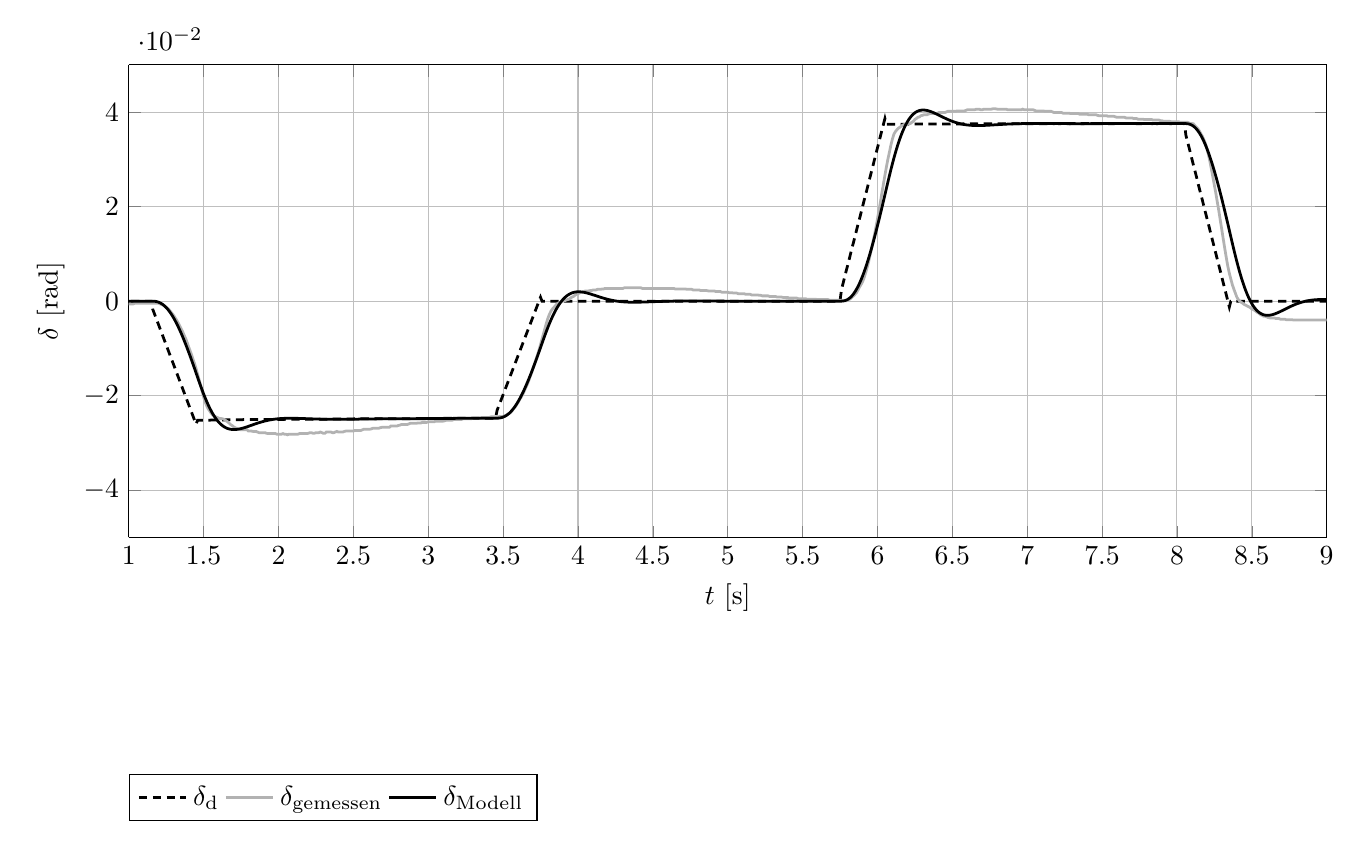
\begin{tikzpicture}

\begin{axis}[%
width=0.95092\figurewidth,
height=\figureheight,
at={(0\figurewidth,0\figureheight)},
scale only axis,
separate axis lines,
every outer x axis line/.append style={black},
every x tick label/.append style={font=\color{black}},
xmin=1,
xmax=9,
xlabel={$t$ [s]},
xmajorgrids,
every outer y axis line/.append style={black},
every y tick label/.append style={font=\color{black}},
ymin=-0.05,
ymax=0.05,
ylabel near ticks,
ylabel={$\delta\text{ [rad]}$},
ymajorgrids,
legend pos=south west,
legend style={legend cell align=left,align=left,draw=black,legend columns=3,at={(0.0,-0.6)}}
]
\addplot [color=black,densely dashed, line width=1]
  table[row sep=crcr]{%
0	1.38725944370566e-016\\
0.00999999999999801	1.38766813710271e-016\\
0.019999999999996	1.38766813710271e-016\\
0.0300000000000011	1.38748086341203e-016\\
0.0399999999999991	1.38748086341203e-016\\
0.0499999999999972	1.3878685133343e-016\\
0.0599999999999952	1.3878685133343e-016\\
0.0700000000000003	1.3882533839297e-016\\
0.0799999999999983	1.3882533839297e-016\\
0.0899999999999963	1.38864129854977e-016\\
0.100000000000001	1.38864129854977e-016\\
0.109999999999999	1.38806690433241e-016\\
0.119999999999997	1.38806690433241e-016\\
0.129999999999995	1.3873098686358e-016\\
0.140000000000001	1.3873098686358e-016\\
0.149999999999999	1.38733713250879e-016\\
0.159999999999997	1.38733713250879e-016\\
0.170000000000002	1.38590286750107e-016\\
0.18	1.38590286750107e-016\\
0.189999999999998	1.38622182834527e-016\\
0.199999999999996	1.38622182834527e-016\\
0.210000000000001	1.38653377469788e-016\\
0.219999999999999	1.38653377469788e-016\\
0.229999999999997	1.38684532400379e-016\\
0.240000000000002	1.38684532400379e-016\\
0.25	1.38628839984097e-016\\
0.259999999999998	1.38628839984097e-016\\
0.269999999999996	1.38604646605541e-016\\
0.280000000000001	1.38604646605541e-016\\
0.289999999999999	1.38485506127554e-016\\
0.299999999999997	1.38485506127554e-016\\
0.309999999999995	1.38498979245371e-016\\
0.32	1.38498979245371e-016\\
0.329999999999998	1.38486353160501e-016\\
0.339999999999996	1.38486353160501e-016\\
0.350000000000001	1.38461220104769e-016\\
0.359999999999999	1.38461220104769e-016\\
0.369999999999997	1.38460809823186e-016\\
0.379999999999995	1.38460809823186e-016\\
0.390000000000001	1.3848444733637e-016\\
0.399999999999999	1.3848444733637e-016\\
0.409999999999997	1.38395005951096e-016\\
0.420000000000002	1.38395005951096e-016\\
0.43	1.38339710581508e-016\\
0.439999999999998	1.38339710581508e-016\\
0.449999999999996	1.38361071693646e-016\\
0.460000000000001	1.38361071693646e-016\\
0.469999999999999	1.38283885816328e-016\\
0.479999999999997	1.38283885816328e-016\\
0.490000000000002	1.38303804325478e-016\\
0.5	1.38303804325478e-016\\
0.509999999999998	1.38323908123086e-016\\
0.519999999999996	1.38323908123086e-016\\
0.530000000000001	1.38348127971421e-016\\
0.539999999999999	1.38348127971421e-016\\
0.549999999999997	1.38259070397951e-016\\
0.559999999999995	1.38259070397951e-016\\
0.57	1.38215527610507e-016\\
0.579999999999998	1.38215527610507e-016\\
0.589999999999996	1.38189838689403e-016\\
0.600000000000001	1.38189838689403e-016\\
0.609999999999999	1.38121983409394e-016\\
0.619999999999997	1.38121983409394e-016\\
0.629999999999995	1.38188184328178e-016\\
0.640000000000001	1.38188184328178e-016\\
0.649999999999999	1.3815616912975e-016\\
0.659999999999997	1.3815616912975e-016\\
0.670000000000002	1.38174499452124e-016\\
0.68	1.38174499452124e-016\\
0.689999999999998	1.38191863627543e-016\\
0.699999999999996	1.38191863627543e-016\\
0.710000000000001	1.3809765768194e-016\\
0.719999999999999	1.3809765768194e-016\\
0.729999999999997	1.38115471843612e-016\\
0.740000000000002	1.38115471843612e-016\\
0.75	1.38113989535954e-016\\
0.759999999999998	1.38113989535954e-016\\
0.769999999999996	1.38117192379286e-016\\
0.780000000000001	1.38117192379286e-016\\
0.789999999999999	1.38122856912121e-016\\
0.799999999999997	1.38122856912121e-016\\
0.809999999999995	1.38140128443311e-016\\
0.82	1.38140128443311e-016\\
0.829999999999998	1.38100714941484e-016\\
0.839999999999996	1.38100714941484e-016\\
0.850000000000001	1.38078056810145e-016\\
0.859999999999999	1.38078056810145e-016\\
0.869999999999997	1.38062969035772e-016\\
0.879999999999995	1.38062969035772e-016\\
0.890000000000001	1.37972018873061e-016\\
0.899999999999999	1.37972018873061e-016\\
0.909999999999997	1.3794811666208e-016\\
0.920000000000002	1.3794811666208e-016\\
0.93	1.3797208504751e-016\\
0.939999999999998	1.3797208504751e-016\\
0.949999999999996	1.37986987533425e-016\\
0.960000000000001	1.37986987533425e-016\\
0.969999999999999	1.37957778131635e-016\\
0.979999999999997	1.37957778131635e-016\\
0.990000000000002	1.37986590486731e-016\\
1	1.37986590486731e-016\\
1.01	1.37861481073444e-016\\
1.02	1.37861481073444e-016\\
1.03	1.37879348174675e-016\\
1.04	1.37879348174675e-016\\
1.05	1.37898856402242e-016\\
1.06	1.37898856402242e-016\\
1.07	1.37811823766911e-016\\
1.08	1.37811823766911e-016\\
1.09	1.37824648375128e-016\\
1.1	1.37824648375128e-016\\
1.11	1.37841191987379e-016\\
1.12	1.37841191987379e-016\\
1.13	1.37751366790301e-016\\
1.14	1.37751366790301e-016\\
1.15	1.37690446592548e-016\\
1.16	-0.00168319279327989\\
1.17	-0.00252507580444217\\
1.18	-0.00336676905862987\\
1.19	-0.00420563062652946\\
1.2	-0.00504676206037402\\
1.21	-0.00588865019381046\\
1.22	-0.00672989897429943\\
1.23	-0.00757259223610163\\
1.24	-0.0084140133112669\\
1.25	-0.00925574079155922\\
1.26	-0.0100972075015306\\
1.27	-0.0109399175271392\\
1.28	-0.0117815006524324\\
1.29	-0.0126150036230683\\
1.3	-0.0134560689330101\\
1.31	-0.0142987323924899\\
1.32	-0.0151399169117212\\
1.33	-0.0159829054027796\\
1.34	-0.0168242193758488\\
1.35	-0.0176675785332918\\
1.36	-0.0185090247541666\\
1.37	-0.0193511005491018\\
1.38	-0.0201926100999117\\
1.39	-0.0210367348045111\\
1.4	-0.021878395229578\\
1.41	-0.0227165464311838\\
1.42	-0.0235581174492836\\
1.43	-0.024389885365963\\
1.44	-0.0252311620861292\\
1.45	-0.0260470118373632\\
1.46	-0.0252077691257\\
1.47	-0.0251978617161512\\
1.48	-0.0251978542655706\\
1.49	-0.0251942183822393\\
1.5	-0.025194214656949\\
1.51	-0.0251967515796423\\
1.52	-0.0251967534422874\\
1.53	-0.0251993183046579\\
1.54	-0.0251993220299482\\
1.55	-0.0251765977591276\\
1.56	-0.0251765828579664\\
1.57	-0.0251500494778156\\
1.58	-0.0251500308513641\\
1.59	-0.0251430813223124\\
1.6	-0.0251430775970221\\
1.61	-0.0251444280147552\\
1.62	-0.0251444280147552\\
1.63	-0.0251308344304562\\
1.64	-0.0251308251172304\\
1.65	-0.0251299701631069\\
1.66	-0.0251299701631069\\
1.67	-0.0251181665807962\\
1.68	-0.0251181554049253\\
1.69	-0.0251189190894365\\
1.7	-0.0251189190894365\\
1.71	-0.0251068063080311\\
1.72	-0.0251067988574505\\
1.73	-0.0250895489007235\\
1.74	-0.0250895339995623\\
1.75	-0.0250896029174328\\
1.76	-0.0250896029174328\\
1.77	-0.0250611752271652\\
1.78	-0.0250611528754234\\
1.79	-0.0250509288161993\\
1.8	-0.0250509213656187\\
1.81	-0.025050338357687\\
1.82	-0.025050338357687\\
1.83	-0.0250519383698702\\
1.84	-0.0250519402325153\\
1.85	-0.0250520445406437\\
1.86	-0.0250520445406437\\
1.87	-0.0250531155616045\\
1.88	-0.0250531155616045\\
1.89	-0.025029681622982\\
1.9	-0.0250296648591757\\
1.91	-0.0250318218022585\\
1.92	-0.0250318218022585\\
1.93	-0.0250322856009007\\
1.94	-0.0250322856009007\\
1.95	-0.0250334590673447\\
1.96	-0.0250334590673447\\
1.97	-0.0250340588390827\\
1.98	-0.0250340607017279\\
1.99	-0.0250277612358332\\
2	-0.0250277556478977\\
2.01	-0.0250296164304018\\
2.02	-0.0250296201556921\\
2.03	-0.0250267926603556\\
2.04	-0.0250267889350653\\
2.05	-0.0250097196549177\\
2.06	-0.0250097084790468\\
2.07	-0.0250140987336636\\
2.08	-0.0250141024589539\\
2.09	-0.0250153001397848\\
2.1	-0.0250153001397848\\
2.11	-0.0250184554606676\\
2.12	-0.0250184554606676\\
2.13	-0.0250216778367758\\
2.14	-0.0250216796994209\\
2.15	-0.0250125285238028\\
2.16	-0.0250125229358673\\
2.17	-0.0250104796141386\\
2.18	-0.0250104796141386\\
2.19	-0.0250127855688334\\
2.2	-0.0250127892941237\\
2.21	-0.0250064563006163\\
2.22	-0.025006452575326\\
2.23	-0.0250084735453129\\
2.24	-0.025008475407958\\
2.25	-0.0250115264207125\\
2.26	-0.0250115264207125\\
2.27	-0.0250150635838509\\
2.28	-0.025015065446496\\
2.29	-0.0250169206410646\\
2.3	-0.0250169206410646\\
2.31	-0.0249876119196415\\
2.32	-0.0249875895678997\\
2.33	-0.0249770991504192\\
2.34	-0.0249770916998386\\
2.35	-0.024980029091239\\
2.36	-0.0249800328165293\\
2.37	-0.024951284751296\\
2.38	-0.0249512642621994\\
2.39	-0.0249548051506281\\
2.4	-0.0249548070132732\\
2.41	-0.024951558560133\\
2.42	-0.0249515566974878\\
2.43	-0.0249455217272043\\
2.44	-0.024945518001914\\
2.45	-0.0249374303966761\\
2.46	-0.0249374248087406\\
2.47	-0.0249229241162539\\
2.48	-0.024922912940383\\
2.49	-0.024925708770752\\
2.5	-0.024925708770752\\
2.51	-0.0249110255390406\\
2.52	-0.0249110125005245\\
2.53	-0.0249148532748222\\
2.54	-0.0249148570001125\\
2.55	-0.0249130353331566\\
2.56	-0.0249130353331566\\
2.57	-0.0249126181006432\\
2.58	-0.0249126181006432\\
2.59	-0.024902019649744\\
2.6	-0.0249020121991634\\
2.61	-0.0249045789241791\\
2.62	-0.0249045789241791\\
2.63	-0.024896802380681\\
2.64	-0.0248967949301004\\
2.65	-0.0248977337032557\\
2.66	-0.0248977337032557\\
2.67	-0.0249009467661381\\
2.68	-0.0249009504914284\\
2.69	-0.0249037742614746\\
2.7	-0.0249037761241198\\
2.71	-0.0249055977910757\\
2.72	-0.0249055977910757\\
2.73	-0.0249058324843645\\
2.74	-0.0249058324843645\\
2.75	-0.0248987805098295\\
2.76	-0.0248987749218941\\
2.77	-0.0248882342129946\\
2.78	-0.024888226762414\\
2.79	-0.024883272126317\\
2.8	-0.0248832684010267\\
2.81	-0.0248767901211977\\
2.82	-0.0248767863959074\\
2.83	-0.0248700156807899\\
2.84	-0.0248700119554996\\
2.85	-0.0248718652874231\\
2.86	-0.0248718671500683\\
2.87	-0.024872774258256\\
2.88	-0.024872774258256\\
2.89	-0.0248555485159159\\
2.9	-0.0248555392026901\\
2.91	-0.0248473901301622\\
2.92	-0.0248473845422268\\
2.93	-0.02484923414886\\
2.94	-0.0248492360115051\\
2.95	-0.0248295236378908\\
2.96	-0.0248295087367296\\
2.97	-0.0248205754905939\\
2.98	-0.0248205661773682\\
2.99	-0.0248233787715435\\
3	-0.0248233787715435\\
3.01	-0.0248213857412338\\
3.02	-0.0248213838785887\\
3.03	-0.024823134765029\\
3.04	-0.024823134765029\\
3.05	-0.0248174350708723\\
3.06	-0.024817431345582\\
3.07	-0.024819815531373\\
3.08	-0.0248198192566633\\
3.09	-0.0247982516884804\\
3.1	-0.0247982386499643\\
3.11	-0.0247992184013128\\
3.12	-0.0247992184013128\\
3.13	-0.0248019769787788\\
3.14	-0.024801978841424\\
3.15	-0.0248056501150131\\
3.16	-0.0248056538403034\\
3.17	-0.0247917771339417\\
3.18	-0.0247917715460062\\
3.19	-0.0247949026525021\\
3.2	-0.0247949026525021\\
3.21	-0.0247856490314007\\
3.22	-0.0247856415808201\\
3.23	-0.0247888527810574\\
3.24	-0.0247888546437025\\
3.25	-0.0247898008674383\\
3.26	-0.0247898008674383\\
3.27	-0.0247849002480507\\
3.28	-0.0247848983854055\\
3.29	-0.0247823316603899\\
3.3	-0.0247823316603899\\
3.31	-0.0247864294797182\\
3.32	-0.0247864313423634\\
3.33	-0.0247864425182343\\
3.34	-0.0247864425182343\\
3.35	-0.024773932993412\\
3.36	-0.0247739236801863\\
3.37	-0.0247776992619038\\
3.38	-0.0247777011245489\\
3.39	-0.02477559261024\\
3.4	-0.0247755888849497\\
3.41	-0.0247652102261782\\
3.42	-0.0247652065008879\\
3.43	-0.0247664321213961\\
3.44	-0.0247664358466864\\
3.45	-0.0247680302709341\\
3.46	-0.0231174398213625\\
3.47	-0.0222903974354267\\
3.48	-0.0214646514505148\\
3.49	-0.0206431429833174\\
3.5	-0.0198172684758902\\
3.51	-0.018988186493516\\
3.52	-0.0181624833494425\\
3.53	-0.0173335503786802\\
3.54	-0.016508037224412\\
3.55	-0.0156750120222569\\
3.56	-0.0148499216884375\\
3.57	-0.0140272444114089\\
3.58	-0.0132020451128483\\
3.59	-0.0123767796903849\\
3.6	-0.0115516064688563\\
3.61	-0.0107263987883925\\
3.62	-0.00990125071257353\\
3.63	-0.00907474663108587\\
3.64	-0.00824973825365305\\
3.65	-0.00742613431066275\\
3.66	-0.00660098856315017\\
3.67	-0.00577646680176258\\
3.68	-0.00495124468579888\\
3.69	-0.0041267448104918\\
3.7	-0.00330138951539993\\
3.71	-0.0024752167519182\\
3.72	-0.00165014201775193\\
3.73	-0.00082456151721999\\
3.74	0\\
3.75	0.000824572693090886\\
3.76	0\\
3.77	1.34931276471536e-016\\
3.78	1.34931276471536e-016\\
3.79	1.34955827192117e-016\\
3.8	1.34955827192117e-016\\
3.81	1.34983818984046e-016\\
3.82	1.34983818984046e-016\\
3.83	1.34974673675193e-016\\
3.84	1.34974673675193e-016\\
3.85	1.34961677013409e-016\\
3.86	1.34961677013409e-016\\
3.87	1.34878442791451e-016\\
3.88	1.34878442791451e-016\\
3.89	1.34871348890518e-016\\
3.9	1.34871348890518e-016\\
3.91	1.34846771700158e-016\\
3.92	1.34846771700158e-016\\
3.93	1.34846771700158e-016\\
3.94	1.34846771700158e-016\\
3.95	1.34867947523839e-016\\
3.96	1.34867947523839e-016\\
3.97	1.34889890971129e-016\\
3.98	1.34889890971129e-016\\
3.99	1.34915275489767e-016\\
4	1.34915275489767e-016\\
4.01	1.34893623210053e-016\\
4.02	1.34893623210053e-016\\
4.03	1.34824629729521e-016\\
4.04	1.34824629729521e-016\\
4.05	1.34847909900681e-016\\
4.06	1.34847909900681e-016\\
4.07	1.34809197848013e-016\\
4.08	1.34809197848013e-016\\
4.09	1.34856883155966e-016\\
4.1	1.34856883155966e-016\\
4.11	1.34817138781894e-016\\
4.12	1.34817138781894e-016\\
4.13	1.34882042681477e-016\\
4.14	1.34882042681477e-016\\
4.15	1.34825410588019e-016\\
4.16	1.34825410588019e-016\\
4.17	1.34796955574947e-016\\
4.18	1.34796955574947e-016\\
4.19	1.34813340368521e-016\\
4.2	1.34813340368521e-016\\
4.21	1.34815841762693e-016\\
4.22	1.34815841762693e-016\\
4.23	1.34874088512707e-016\\
4.24	1.34874088512707e-016\\
4.25	1.34820235746107e-016\\
4.26	1.34820235746107e-016\\
4.27	1.34855467022757e-016\\
4.28	1.34855467022757e-016\\
4.29	1.34832054502699e-016\\
4.3	1.34832054502699e-016\\
4.31	1.3487122977651e-016\\
4.32	1.3487122977651e-016\\
4.33	1.34827938451971e-016\\
4.34	1.34827938451971e-016\\
4.35	1.34872434151482e-016\\
4.36	1.34872434151482e-016\\
4.37	1.34845673204304e-016\\
4.38	1.34845673204304e-016\\
4.39	1.348572272631e-016\\
4.4	1.348572272631e-016\\
4.41	1.34906222825143e-016\\
4.42	1.34906222825143e-016\\
4.43	1.34905336087527e-016\\
4.44	1.34905336087527e-016\\
4.45	1.34961107913147e-016\\
4.46	1.34961107913147e-016\\
4.47	1.34905931657568e-016\\
4.48	1.34905931657568e-016\\
4.49	1.34925241361787e-016\\
4.5	1.34925241361787e-016\\
4.51	1.34920159164103e-016\\
4.52	1.34920159164103e-016\\
4.53	1.34975454533691e-016\\
4.54	1.34975454533691e-016\\
4.55	1.34996590652703e-016\\
4.56	1.34996590652703e-016\\
4.57	1.34981291120094e-016\\
4.58	1.34981291120094e-016\\
4.59	1.34992593715984e-016\\
4.6	1.34992593715984e-016\\
4.61	1.35049040520984e-016\\
4.62	1.35049040520984e-016\\
4.63	1.35017091497005e-016\\
4.64	1.35017091497005e-016\\
4.65	1.35021313426851e-016\\
4.66	1.35021313426851e-016\\
4.67	1.35045109758713e-016\\
4.68	1.35045109758713e-016\\
4.69	1.35021551654868e-016\\
4.7	1.35021551654868e-016\\
4.71	1.35047743501784e-016\\
4.72	1.35047743501784e-016\\
4.73	1.3506062104956e-016\\
4.74	1.3506062104956e-016\\
4.75	1.35122202991803e-016\\
4.76	1.35122202991803e-016\\
4.77	1.35134286446191e-016\\
4.78	1.35134286446191e-016\\
4.79	1.35060660754229e-016\\
4.8	1.35060660754229e-016\\
4.81	1.3508387475094e-016\\
4.82	1.3508387475094e-016\\
4.83	1.35079996928228e-016\\
4.84	1.35079996928228e-016\\
4.85	1.35165428141893e-016\\
4.86	1.35165428141893e-016\\
4.87	1.35106294654263e-016\\
4.88	1.35106294654263e-016\\
4.89	1.35149493334573e-016\\
4.9	1.35149493334573e-016\\
4.91	1.35126967552132e-016\\
4.92	1.35126967552132e-016\\
4.93	1.35192572900874e-016\\
4.94	1.35192572900874e-016\\
4.95	1.35129918932557e-016\\
4.96	1.35129918932557e-016\\
4.97	1.35142439138309e-016\\
4.98	1.35142439138309e-016\\
4.99	1.35177035140248e-016\\
5	1.35177035140248e-016\\
5.01	1.35153371157284e-016\\
5.02	1.35153371157284e-016\\
5.03	1.35234527501543e-016\\
5.04	1.35234527501543e-016\\
5.05	1.35193869920075e-016\\
5.06	1.35193869920075e-016\\
5.07	1.35254790117828e-016\\
5.08	1.35254790117828e-016\\
5.09	1.35242772837889e-016\\
5.1	1.35242772837889e-016\\
5.11	1.35229101196725e-016\\
5.12	1.35229101196725e-016\\
5.13	1.3523141730244e-016\\
5.14	1.3523141730244e-016\\
5.15	1.35256338599935e-016\\
5.16	1.35256338599935e-016\\
5.17	1.35279407012858e-016\\
5.18	1.35279407012858e-016\\
5.19	1.35243831629073e-016\\
5.2	1.35243831629073e-016\\
5.21	1.35332320102281e-016\\
5.22	1.35332320102281e-016\\
5.23	1.35336303804112e-016\\
5.24	1.35336303804112e-016\\
5.25	1.35301496043935e-016\\
5.26	1.35301496043935e-016\\
5.27	1.35317073509231e-016\\
5.28	1.35317073509231e-016\\
5.29	1.35338646379606e-016\\
5.3	1.35338646379606e-016\\
5.31	1.35418611583783e-016\\
5.32	1.35418611583783e-016\\
5.33	1.35410405952106e-016\\
5.34	1.35410405952106e-016\\
5.35	1.35421708547996e-016\\
5.36	1.35421708547996e-016\\
5.37	1.35433937586172e-016\\
5.38	1.35433937586172e-016\\
5.39	1.35481106733423e-016\\
5.4	1.35481106733423e-016\\
5.41	1.35469102688373e-016\\
5.42	1.35469102688373e-016\\
5.43	1.35464973402755e-016\\
5.44	1.35464973402755e-016\\
5.45	1.35504638367489e-016\\
5.46	1.35504638367489e-016\\
5.47	1.35519779081421e-016\\
5.48	1.35519779081421e-016\\
5.49	1.35578065536104e-016\\
5.5	1.35578065536104e-016\\
5.51	1.35590612211635e-016\\
5.52	1.35590612211635e-016\\
5.53	1.35614461483056e-016\\
5.54	1.35614461483056e-016\\
5.55	1.35634075589741e-016\\
5.56	1.35634075589741e-016\\
5.57	1.35645060548276e-016\\
5.58	1.35645060548276e-016\\
5.59	1.35637979882232e-016\\
5.6	1.35637979882232e-016\\
5.61	1.3564543112519e-016\\
5.62	1.3564543112519e-016\\
5.63	1.35684738747898e-016\\
5.64	1.35684738747898e-016\\
5.65	1.35673184689102e-016\\
5.66	1.35673184689102e-016\\
5.67	1.3578032112204e-016\\
5.68	1.3578032112204e-016\\
5.69	1.35787600311431e-016\\
5.7	1.35787600311431e-016\\
5.71	1.35736381287901e-016\\
5.72	1.35736381287901e-016\\
5.73	1.35783616609601e-016\\
5.74	1.35783616609601e-016\\
5.75	1.35782796046433e-016\\
5.76	0.00245660915970802\\
5.77	0.00368707999587059\\
5.78	0.00498254224658012\\
5.79	0.00624298397451639\\
5.8	0.0074384668841958\\
5.81	0.00867043156176806\\
5.82	0.00996604189276695\\
5.83	0.0112340282648802\\
5.84	0.0124306194484234\\
5.85	0.0136608853936195\\
5.86	0.0149572547525167\\
5.87	0.0162162110209465\\
5.88	0.0174130797386169\\
5.89	0.0186487417668104\\
5.9	0.019941434264183\\
5.91	0.0211933236569166\\
5.92	0.0224109590053558\\
5.93	0.0236469935625792\\
5.94	0.0249325875192881\\
5.95	0.0261870045214891\\
5.96	0.02741121314466\\
5.97	0.0286500584334135\\
5.98	0.0299318917095661\\
5.99	0.0311878342181444\\
6	0.0324172414839268\\
6.01	0.0336417630314827\\
6.02	0.0349307283759117\\
6.03	0.0361873805522919\\
6.04	0.0374184548854828\\
6.05	0.0386564619839191\\
6.06	0.0374276675283909\\
6.07	0.0374386310577393\\
6.08	0.0374386496841908\\
6.09	0.0374365150928497\\
6.1	0.0374365076422691\\
6.11	0.037445455789566\\
6.12	0.0374454706907272\\
6.13	0.0374514497816563\\
6.14	0.0374514609575272\\
6.15	0.0374540984630585\\
6.16	0.0374540984630585\\
6.17	0.0374520644545555\\
6.18	0.0374520570039749\\
6.19	0.0374608859419823\\
6.2	0.0374608971178532\\
6.21	0.0374642610549927\\
6.22	0.037464264780283\\
6.23	0.0374734066426754\\
6.24	0.0374734252691269\\
6.25	0.0374756082892418\\
6.26	0.0374756082892418\\
6.27	0.0374830365180969\\
6.28	0.0374830476939678\\
6.29	0.0374876484274864\\
6.3	0.0374876596033573\\
6.31	0.0374681614339352\\
6.32	0.0374681353569031\\
6.33	0.0374891124665737\\
6.34	0.0374891459941864\\
6.35	0.0374921075999737\\
6.36	0.0374921150505543\\
6.37	0.0374836586415768\\
6.38	0.0374836400151253\\
6.39	0.0374913327395916\\
6.4	0.0374913439154625\\
6.41	0.0374819897115231\\
6.42	0.0374819785356522\\
6.43	0.03749905154109\\
6.44	0.0374990850687027\\
6.45	0.0375012680888176\\
6.46	0.0375012755393982\\
6.47	0.037485770881176\\
6.48	0.0374857448041439\\
6.49	0.0375045388936996\\
6.5	0.037504568696022\\
6.51	0.0375087931752205\\
6.52	0.0375088006258011\\
6.53	0.0375001356005669\\
6.54	0.0375001206994057\\
6.55	0.0375151969492435\\
6.56	0.0375152193009853\\
6.57	0.0375194996595383\\
6.58	0.0375195071101189\\
6.59	0.0375288128852844\\
6.6	0.0375288240611553\\
6.61	0.0375287719070911\\
6.62	0.0375287719070911\\
6.63	0.0375222377479076\\
6.64	0.0375222228467464\\
6.65	0.0375341475009918\\
6.66	0.0375341661274433\\
6.67	0.0375162363052368\\
6.68	0.0375162065029144\\
6.69	0.0375388376414776\\
6.7	0.0375388786196709\\
6.71	0.0375444293022156\\
6.72	0.0375444442033768\\
6.73	0.0375351272523403\\
6.74	0.0375351123511791\\
6.75	0.0375455133616924\\
6.76	0.0375455319881439\\
6.77	0.0375355891883373\\
6.78	0.0375355705618858\\
6.79	0.0375406034290791\\
6.8	0.0375406183302403\\
6.81	0.0375522002577782\\
6.82	0.0375522188842297\\
6.83	0.0375510938465595\\
6.84	0.0375510901212692\\
6.85	0.0375560633838177\\
6.86	0.0375560708343983\\
6.87	0.0375610999763012\\
6.88	0.0375611111521721\\
6.89	0.0375638641417027\\
6.9	0.037563867866993\\
6.91	0.0375544466078281\\
6.92	0.0375544279813766\\
6.93	0.0375544205307961\\
6.94	0.0375544205307961\\
6.95	0.0375536791980267\\
6.96	0.0375536791980267\\
6.97	0.0375510901212692\\
6.98	0.0375510901212692\\
6.99	0.0375646352767944\\
7	0.0375646576285362\\
7.01	0.0375605151057243\\
7.02	0.0375605076551437\\
7.03	0.0375755690038204\\
7.04	0.0375755950808525\\
7.05	0.0375698879361153\\
7.06	0.0375698804855347\\
7.07	0.037564430385828\\
7.08	0.0375644229352474\\
7.09	0.0375745035707951\\
7.1	0.0375745184719563\\
7.11	0.0375583320856094\\
7.12	0.0375583060085773\\
7.13	0.0375744178891182\\
7.14	0.0375744439661503\\
7.15	0.0375727452337742\\
7.16	0.0375727415084839\\
7.17	0.0375716388225555\\
7.18	0.0375716350972652\\
7.19	0.0375917591154575\\
7.2	0.0375917926430702\\
7.21	0.0375705398619175\\
7.22	0.0375705063343048\\
7.23	0.0375710912048817\\
7.24	0.0375710912048817\\
7.25	0.0375733263790607\\
7.26	0.037573330104351\\
7.27	0.0375569649040699\\
7.28	0.0375569388270378\\
7.29	0.0375782400369644\\
7.3	0.0375782772898674\\
7.31	0.037579357624054\\
7.32	0.037579357624054\\
7.33	0.0375860333442688\\
7.34	0.0375860407948494\\
7.35	0.0375756174325943\\
7.36	0.0375756025314331\\
7.37	0.0375733599066734\\
7.38	0.0375733561813831\\
7.39	0.0375844798982143\\
7.4	0.0375844985246658\\
7.41	0.0375800095498562\\
7.42	0.0375800020992756\\
7.43	0.0375729911029339\\
7.44	0.0375729762017727\\
7.45	0.037580031901598\\
7.46	0.0375800393521786\\
7.47	0.0375956557691097\\
7.48	0.0375956781208515\\
7.49	0.037584912031889\\
7.5	0.0375848971307278\\
7.51	0.0375822596251965\\
7.52	0.0375822558999062\\
7.53	0.0375766828656197\\
7.54	0.0375766716897488\\
7.55	0.0375693440437317\\
7.56	0.0375693365931511\\
7.57	0.0375726781785488\\
7.58	0.0375726819038391\\
7.59	0.0375834479928017\\
7.6	0.0375834666192532\\
7.61	0.0375911332666874\\
7.62	0.0375911444425583\\
7.63	0.0376010574400425\\
7.64	0.0376010723412037\\
7.65	0.0375848934054375\\
7.66	0.0375848673284054\\
7.67	0.0375767350196838\\
7.68	0.0375767201185226\\
7.69	0.0376012027263641\\
7.7	0.0376012399792671\\
7.71	0.037571519613266\\
7.72	0.0375714711844921\\
7.73	0.0375725999474525\\
7.74	0.0375726036727428\\
7.75	0.0375715345144272\\
7.76	0.0375715270638466\\
7.77	0.0375803560018539\\
7.78	0.0375803746283054\\
7.79	0.0375834442675114\\
7.8	0.0375834479928017\\
7.81	0.0375785529613495\\
7.82	0.0375785455107689\\
7.83	0.0375756286084652\\
7.84	0.0375756211578846\\
7.85	0.0375778637826443\\
7.86	0.0375778675079346\\
7.87	0.0375566110014915\\
7.88	0.0375565774738789\\
7.89	0.0375878624618053\\
7.9	0.0375879108905792\\
7.91	0.0375856570899487\\
7.92	0.0375856533646584\\
7.93	0.0375791266560555\\
7.94	0.0375791117548943\\
7.95	0.037575613707304\\
7.96	0.0375756099820137\\
7.97	0.0375739894807339\\
7.98	0.0375739894807339\\
7.99	0.037573903799057\\
8	0.037573903799057\\
8.01	0.0375812388956547\\
8.02	0.0375812537968159\\
8.03	0.0375896021723747\\
8.04	0.0375896133482456\\
8.05	0.037572342902422\\
8.06	0.0351007953286171\\
8.07	0.0338788330554962\\
8.08	0.0326407216489315\\
8.09	0.0313958637416363\\
8.1	0.0300913080573082\\
8.11	0.0288157314062119\\
8.12	0.0276117268949747\\
8.13	0.0263731963932514\\
8.14	0.0250691846013069\\
8.15	0.0238000005483627\\
8.16	0.0225854441523552\\
8.17	0.0213533919304609\\
8.18	0.0200679954141378\\
8.19	0.0188131742179394\\
8.2	0.0175791643559933\\
8.21	0.0163464229553938\\
8.22	0.0150637309998274\\
8.23	0.013805728405714\\
8.24	0.012564716860652\\
8.25	0.0113221034407616\\
8.26	0.0100487535819411\\
8.27	0.0087902033701539\\
8.28	0.00754886912181973\\
8.29	0.00631502782925963\\
8.3	0.00503526069223881\\
8.31	0.00377762690186501\\
8.32	0.00253930292092264\\
8.33	0.00130341411568224\\
8.34	2.39882501773536e-005\\
8.35	-0.00123366096522659\\
8.36	0\\
8.37	1.36649429865482e-016\\
8.38	1.36649429865482e-016\\
8.39	1.36703362041421e-016\\
8.4	1.36703362041421e-016\\
8.41	1.36625130607808e-016\\
8.42	1.36625130607808e-016\\
8.43	1.366575825576e-016\\
8.44	1.366575825576e-016\\
8.45	1.36639331644564e-016\\
8.46	1.36639331644564e-016\\
8.47	1.36637518464662e-016\\
8.48	1.36637518464662e-016\\
8.49	1.36752979643284e-016\\
8.5	1.36752979643284e-016\\
8.51	1.36699537158268e-016\\
8.52	1.36699537158268e-016\\
8.53	1.36664332351398e-016\\
8.54	1.36664332351398e-016\\
8.55	1.36615919124507e-016\\
8.56	1.36615919124507e-016\\
8.57	1.36623317427905e-016\\
8.58	1.36623317427905e-016\\
8.59	1.36622298341391e-016\\
8.6	1.36622298341391e-016\\
8.61	1.36646213787261e-016\\
8.62	1.36646213787261e-016\\
8.63	1.3664025808685e-016\\
8.64	1.3664025808685e-016\\
8.65	1.36696347549826e-016\\
8.66	1.36696347549826e-016\\
8.67	1.36706472240524e-016\\
8.68	1.36706472240524e-016\\
8.69	1.36656431122187e-016\\
8.7	1.36656431122187e-016\\
8.71	1.3659838289552e-016\\
8.72	1.3659838289552e-016\\
8.73	1.36648185785841e-016\\
8.74	1.36648185785841e-016\\
8.75	1.36685018484157e-016\\
8.76	1.36685018484157e-016\\
8.77	1.36637319941315e-016\\
8.78	1.36637319941315e-016\\
8.79	1.36675317309933e-016\\
8.8	1.36675317309933e-016\\
8.81	1.36686964012958e-016\\
8.82	1.36686964012958e-016\\
8.83	1.36675171726145e-016\\
8.84	1.36675171726145e-016\\
8.85	1.36603478328094e-016\\
8.86	1.36603478328094e-016\\
8.87	1.36593155114049e-016\\
8.88	1.36593155114049e-016\\
8.89	1.36598197607063e-016\\
8.9	1.36598197607063e-016\\
8.91	1.36629789289018e-016\\
8.92	1.36629789289018e-016\\
8.93	1.36604166542363e-016\\
8.94	1.36604166542363e-016\\
8.95	1.36644003560664e-016\\
8.96	1.36644003560664e-016\\
8.97	1.36658641348784e-016\\
8.98	1.36658641348784e-016\\
8.99	1.36567757360521e-016\\
9	1.36567757360521e-016\\
9.01	1.36563601605124e-016\\
9.02	1.36563601605124e-016\\
9.03	1.3659177868551e-016\\
9.04	1.3659177868551e-016\\
9.05	1.36649218107246e-016\\
9.06	1.36649218107246e-016\\
9.07	1.36696453428945e-016\\
9.08	1.36696453428945e-016\\
9.09	1.36617586720621e-016\\
9.1	1.36617586720621e-016\\
9.11	1.3667216740616e-016\\
9.12	1.3667216740616e-016\\
9.13	1.36673067378667e-016\\
9.14	1.36673067378667e-016\\
9.15	1.36620829268623e-016\\
9.16	1.36620829268623e-016\\
9.17	1.36660123656441e-016\\
9.18	1.36660123656441e-016\\
9.19	1.36629365772544e-016\\
9.2	1.36629365772544e-016\\
9.21	1.36684369974557e-016\\
9.22	1.36684369974557e-016\\
9.23	1.36673451190471e-016\\
9.24	1.36673451190471e-016\\
9.25	1.36687427234101e-016\\
9.26	1.36687427234101e-016\\
9.27	1.36631774522488e-016\\
9.28	1.36631774522488e-016\\
9.29	1.36575393891936e-016\\
9.3	1.36575393891936e-016\\
9.31	1.36615588252262e-016\\
9.32	1.36615588252262e-016\\
9.33	1.36576042401537e-016\\
9.34	1.36576042401537e-016\\
9.35	1.36595391810425e-016\\
9.36	1.36595391810425e-016\\
9.37	1.36635758224318e-016\\
9.38	1.36635758224318e-016\\
9.39	1.36658310476539e-016\\
9.4	1.36658310476539e-016\\
9.41	1.36651865085206e-016\\
9.42	1.36651865085206e-016\\
9.43	1.36583387765376e-016\\
9.44	1.36583387765376e-016\\
9.45	1.36583493644494e-016\\
9.46	1.36583493644494e-016\\
9.47	1.36631999515615e-016\\
9.48	1.36631999515615e-016\\
9.49	1.36575737999071e-016\\
9.5	1.36575737999071e-016\\
9.51	1.36576346804002e-016\\
9.52	1.36576346804002e-016\\
9.53	1.36664239707169e-016\\
9.54	1.36664239707169e-016\\
9.55	1.366363008548e-016\\
9.56	1.366363008548e-016\\
9.57	1.36655901726595e-016\\
9.58	1.36655901726595e-016\\
9.59	1.36647934322935e-016\\
9.6	1.36647934322935e-016\\
9.61	1.36584367147221e-016\\
9.62	1.36584367147221e-016\\
9.63	1.36623807118828e-016\\
9.64	1.36623807118828e-016\\
9.65	1.36643447695292e-016\\
9.66	1.36643447695292e-016\\
9.67	1.36648304899849e-016\\
9.68	1.36648304899849e-016\\
9.69	1.36662108889912e-016\\
9.7	1.36662108889912e-016\\
9.71	1.36657781080947e-016\\
9.72	1.36657781080947e-016\\
9.73	1.36584565670568e-016\\
9.74	1.36584565670568e-016\\
9.75	1.36519436777858e-016\\
9.76	1.36519436777858e-016\\
9.77	1.36543550747076e-016\\
9.78	1.36543550747076e-016\\
9.79	1.36559631138184e-016\\
9.8	1.36559631138184e-016\\
9.81	1.36571621948343e-016\\
9.82	1.36571621948343e-016\\
9.83	1.36601479859734e-016\\
9.84	1.36601479859734e-016\\
9.85	1.36582342209082e-016\\
9.86	1.36582342209082e-016\\
9.87	1.36608586995557e-016\\
9.88	1.36608586995557e-016\\
9.89	1.36523142547003e-016\\
9.9	1.36523142547003e-016\\
9.91	1.36521858762692e-016\\
9.92	1.36521858762692e-016\\
9.93	1.36538733247188e-016\\
9.94	1.36538733247188e-016\\
9.95	1.36536020094779e-016\\
9.96	1.36536020094779e-016\\
9.97	1.36559670842853e-016\\
9.98	1.36559670842853e-016\\
9.99	1.36577868816329e-016\\
10	1.36577868816329e-016\\
10.01	1.36591236055028e-016\\
10.02	1.36591236055028e-016\\
10.03	1.36523566063476e-016\\
10.04	1.36523566063476e-016\\
10.05	1.36506426881184e-016\\
10.06	1.36506426881184e-016\\
10.07	1.36514539868632e-016\\
10.08	1.36514539868632e-016\\
10.09	1.36515611894706e-016\\
10.1	1.36515611894706e-016\\
10.11	1.36493377279841e-016\\
10.12	1.36493377279841e-016\\
10.13	1.36506943041886e-016\\
10.14	1.36506943041886e-016\\
10.15	1.36515386901579e-016\\
10.16	1.36515386901579e-016\\
10.17	1.36509576784957e-016\\
10.18	1.36509576784957e-016\\
10.19	1.36491537630158e-016\\
10.2	1.36491537630158e-016\\
10.21	1.36487725981896e-016\\
10.22	1.36487725981896e-016\\
10.23	1.36483265824033e-016\\
10.24	1.36483265824033e-016\\
10.25	1.36483517286939e-016\\
10.26	1.36483517286939e-016\\
10.27	1.36471261778983e-016\\
10.28	1.36471261778983e-016\\
10.29	1.36519516187197e-016\\
10.3	1.36519516187197e-016\\
10.31	1.36507406263029e-016\\
10.32	1.36507406263029e-016\\
10.33	1.36477627760978e-016\\
10.34	1.36477627760978e-016\\
10.35	1.36446631649064e-016\\
10.36	-0.00373627920635045\\
10.37	-0.0055990070104599\\
10.38	-0.00671787280589342\\
10.39	-0.00796815659850836\\
10.4	-0.00935861095786095\\
10.41	-0.0109490882605314\\
10.42	-0.0126750515773892\\
10.43	-0.0144499987363815\\
10.44	-0.0162585489451885\\
10.45	-0.0180881693959236\\
10.46	-0.0199340973049402\\
10.47	-0.0217901393771172\\
10.48	-0.0236435178667307\\
10.49	-0.0255161803215742\\
10.5	-0.0274026766419411\\
10.51	-0.0292807854712009\\
10.52	-0.0311545561999083\\
10.53	-0.0330259539186955\\
10.54	-0.0348965302109718\\
10.55	-0.0367651656270027\\
10.56	-0.0386302843689919\\
10.57	-0.0405109003186226\\
10.58	-0.0424072816967964\\
10.59	-0.0442925207316875\\
10.6	-0.0461753830313683\\
10.61	-0.0480544827878475\\
10.62	-0.0499332174658775\\
10.63	-0.0518102496862412\\
10.64	-0.0536795556545258\\
10.65	-0.0555620416998863\\
10.66	-0.0554117411375046\\
10.67	-0.0559797435998917\\
10.68	-0.0562806166708469\\
10.69	-0.0563601851463318\\
10.7	-0.0563601218163967\\
10.71	-0.0563718117773533\\
10.72	-0.0563718490302563\\
10.73	-0.0563835091888905\\
10.74	-0.056383553892374\\
10.75	-0.0563803054392338\\
10.76	-0.056380283087492\\
10.77	-0.0563582926988602\\
10.78	-0.0563582107424736\\
10.79	-0.0563437417149544\\
10.8	-0.0563436932861805\\
10.81	-0.0563265606760979\\
10.82	-0.0563264936208725\\
10.83	-0.0562979355454445\\
10.84	-0.0562978349626064\\
10.85	-0.0563087239861488\\
10.86	-0.0563087612390518\\
10.87	-0.0563199259340763\\
10.88	-0.0563199669122696\\
10.89	-0.0563169717788696\\
10.9	-0.056316964328289\\
10.91	-0.0563020557165146\\
10.92	-0.0563019998371601\\
10.93	-0.0562842078506947\\
10.94	-0.0562841407954693\\
10.95	-0.0562662594020367\\
10.96	-0.0562661997973919\\
10.97	-0.0562803037464619\\
10.98	-0.0562803447246552\\
10.99	-0.056250337511301\\
11	-0.0562502220273018\\
11.01	-0.056256890296936\\
11.02	-0.0562569089233875\\
11.03	-0.056245282292366\\
11.04	-0.056245245039463\\
11.05	-0.0562420636415482\\
11.06	-0.0562420524656773\\
11.07	-0.0562496855854988\\
11.08	-0.0562497116625309\\
11.09	-0.0562276691198349\\
11.1	-0.0562275908887386\\
11.11	-0.0562248937785625\\
11.12	-0.0562248826026917\\
11.13	-0.0562377162277699\\
11.14	-0.056237768381834\\
11.15	-0.0562494173645973\\
11.16	-0.0562494620680809\\
11.17	-0.0562558360397816\\
11.18	-0.0562558583915234\\
11.19	-0.0562343709170818\\
11.2	-0.0562342889606953\\
11.21	-0.0562452673912048\\
11.22	-0.0562453046441078\\
11.23	-0.0562288016080856\\
11.24	-0.0562287457287312\\
11.25	-0.0561961382627487\\
11.26	-0.0561960153281689\\
11.27	-0.0562216974794865\\
11.28	-0.0562217906117439\\
11.29	-0.0562136769294739\\
11.3	-0.0562136471271515\\
11.31	-0.0562260374426842\\
11.32	-0.0562260821461678\\
11.33	-0.0562228225171566\\
11.34	-0.0562228076159954\\
11.35	-0.0562100894749165\\
11.36	-0.0562100373208523\\
11.37	-0.0562050528824329\\
11.38	-0.0562050379812717\\
11.39	-0.056193470954895\\
11.4	-0.0561934299767017\\
11.41	-0.0561595410108566\\
11.42	-0.0561594180762768\\
11.43	-0.0561517812311649\\
11.44	-0.0561517551541328\\
11.45	-0.0561628788709641\\
11.46	-0.056162916123867\\
11.47	-0.0561750493943691\\
11.48	-0.0561750866472721\\
11.49	-0.0561703257262707\\
11.5	-0.0561703033745289\\
11.51	-0.0561448112130165\\
11.52	-0.056144718080759\\
11.53	-0.0561553537845612\\
11.54	-0.0561553947627544\\
11.55	-0.0561665259301662\\
11.56	-0.0561665594577789\\
11.57	-0.0561450943350792\\
11.58	-0.0561450123786926\\
11.59	-0.0561568848788738\\
11.6	-0.0561569258570671\\
11.61	-0.0561672374606133\\
11.62	-0.0561672747135162\\
11.63	-0.0561777874827385\\
11.64	-0.0561778247356415\\
11.65	-0.0561383776366711\\
11.66	-0.0561382360756397\\
11.67	-0.056149672716856\\
11.68	-0.0561497136950493\\
11.69	-0.0561184547841549\\
11.7	-0.0561183504760265\\
11.71	-0.0561195947229862\\
11.72	-0.0561196021735668\\
11.73	-0.0561166889965534\\
11.74	-0.0561166852712631\\
11.75	-0.0560826286673546\\
11.76	-0.056082509458065\\
11.77	-0.0560824312269688\\
11.78	-0.0560824312269688\\
11.79	-0.0560789257287979\\
11.8	-0.056078914552927\\
11.81	-0.0560807920992374\\
11.82	-0.056080799549818\\
11.83	-0.0560836307704449\\
11.84	-0.0560836419463158\\
11.85	-0.0560953877866268\\
11.86	-0.0560954250395298\\
11.87	-0.0560612082481384\\
11.88	-0.0560610890388489\\
11.89	-0.0560729093849659\\
11.9	-0.0560729466378689\\
11.91	-0.0560845956206322\\
11.92	-0.0560846440494061\\
11.93	-0.0560969263315201\\
11.94	-0.0560969673097134\\
11.95	-0.056082159280777\\
11.96	-0.0560821034014225\\
11.97	-0.0560644865036011\\
11.98	-0.0560644306242466\\
11.99	-0.0560695640742779\\
12	-0.0560695864260197\\
12.01	-0.0560753047466278\\
12.02	-0.0560753270983696\\
12.03	-0.0560552962124348\\
12.04	-0.0560552254319191\\
12.05	-0.0560411736369133\\
12.06	-0.0560411289334297\\
12.07	-0.0560265555977821\\
12.08	-0.0560265071690083\\
12.09	-0.0560382306575775\\
12.1	-0.0560382716357708\\
12.11	-0.0560458153486252\\
12.12	-0.0560458414256573\\
12.13	-0.0560447610914707\\
12.14	-0.0560447610914707\\
12.15	-0.0560515113174915\\
12.16	-0.0560515336692333\\
12.17	-0.0560156144201756\\
12.18	-0.0560154914855957\\
12.19	-0.0560279339551926\\
12.2	-0.0560279749333858\\
12.21	-0.0560228824615479\\
12.22	-0.0560228638350964\\
12.23	-0.0559941790997982\\
12.24	-0.0559940785169601\\
12.25	-0.055989645421505\\
12.26	-0.0559896305203438\\
12.27	-0.0559989996254444\\
12.28	-0.0559990257024765\\
12.29	-0.0559960640966892\\
12.3	-0.0559960529208183\\
12.31	-0.0560056753456593\\
12.32	-0.0560057163238525\\
12.33	-0.0560102909803391\\
12.34	-0.0560103096067905\\
12.35	-0.0559851378202438\\
12.36	-0.055985052138567\\
12.37	-0.0559719316661358\\
12.38	-0.0559718869626522\\
12.39	-0.0559841208159924\\
12.4	-0.0559841617941856\\
12.41	-0.0559756867587566\\
12.42	-0.0559756569564343\\
12.43	-0.0559872649610043\\
12.44	-0.0559873059391975\\
12.45	-0.0559718273580074\\
12.46	-0.055971771478653\\
12.47	-0.0559807159006596\\
12.48	-0.0559807494282722\\
12.49	-0.0559769235551357\\
12.5	-0.0559769049286842\\
12.51	-0.0559394173324108\\
12.52	-0.0559392906725407\\
12.53	-0.0559734702110291\\
12.54	-0.0559735856950283\\
12.55	-0.0559402480721474\\
12.56	-0.0559401363134384\\
12.57	-0.0559685342013836\\
12.58	-0.0559686347842216\\
12.59	-0.0559473745524883\\
12.6	-0.0559473000466824\\
12.61	-0.0559488721191883\\
12.62	-0.0559488758444786\\
12.63	-0.0559625923633575\\
12.64	-0.0559626445174217\\
12.65	-0.0559407398104668\\
12.66	-0.0522359572350979\\
12.67	-0.0503794439136982\\
12.68	-0.0492436289787292\\
12.69	-0.0480041727423668\\
12.7	-0.0465705059468746\\
12.71	-0.0449943952262402\\
12.72	-0.0432867296040058\\
12.73	-0.0415302366018295\\
12.74	-0.0397384315729141\\
12.75	-0.0379231348633766\\
12.76	-0.0360992327332497\\
12.77	-0.0342531651258469\\
12.78	-0.0323831774294376\\
12.79	-0.0305174924433231\\
12.8	-0.0286555141210556\\
12.81	-0.0267962105572224\\
12.82	-0.0249366573989391\\
12.83	-0.0230776481330395\\
12.84	-0.0212265327572823\\
12.85	-0.0193619877099991\\
12.86	-0.0174830295145512\\
12.87	-0.0156135857105255\\
12.88	-0.0137491729110479\\
12.89	-0.0118880439549685\\
12.9	-0.0100290775299072\\
12.91	-0.00817177724093199\\
12.92	-0.00632078293710947\\
12.93	-0.00445604976266623\\
12.94	-0.00257748225703835\\
12.95	-0.000708732870407403\\
12.96	-0.000910224334802479\\
12.97	-0.000354825373506173\\
12.98	-7.12920009391382e-005\\
12.99	1.35395728459317e-016\\
13	1.35395728459317e-016\\
13.01	1.35371971832125e-016\\
13.02	1.35371971832125e-016\\
13.03	1.35379343665744e-016\\
13.04	1.35379343665744e-016\\
13.05	1.35414376419047e-016\\
13.06	1.35414376419047e-016\\
13.07	1.35453511988188e-016\\
13.08	1.35453511988188e-016\\
13.09	1.35398798953751e-016\\
13.1	1.35398798953751e-016\\
13.11	1.35467276273581e-016\\
13.12	1.35467276273581e-016\\
13.13	1.35400625368544e-016\\
13.14	1.35400625368544e-016\\
13.15	1.35476699515119e-016\\
13.16	1.35476699515119e-016\\
13.17	1.35414892579749e-016\\
13.18	1.35414892579749e-016\\
13.19	1.35440647675301e-016\\
13.2	1.35440647675301e-016\\
13.21	1.35468520353222e-016\\
13.22	1.35468520353222e-016\\
13.23	1.35422330587817e-016\\
13.24	1.35422330587817e-016\\
13.25	1.35438265395137e-016\\
13.26	1.35438265395137e-016\\
13.27	1.3544741070399e-016\\
13.28	1.3544741070399e-016\\
13.29	1.35475865717061e-016\\
13.3	1.35475865717061e-016\\
13.31	1.35418254241758e-016\\
13.32	1.35418254241758e-016\\
13.33	1.35453644337086e-016\\
13.34	1.35453644337086e-016\\
13.35	1.35476474521992e-016\\
13.36	1.35476474521992e-016\\
13.37	1.3538754929742e-016\\
13.38	1.3538754929742e-016\\
13.39	1.35383658239819e-016\\
13.4	1.35383658239819e-016\\
13.41	1.35389918342695e-016\\
13.42	1.35389918342695e-016\\
13.43	1.35399301879564e-016\\
13.44	1.35399301879564e-016\\
13.45	1.35392657964884e-016\\
13.46	1.35392657964884e-016\\
13.47	1.35411147105935e-016\\
13.48	1.35411147105935e-016\\
13.49	1.35422409997156e-016\\
13.5	1.35422409997156e-016\\
13.51	1.35375505547702e-016\\
13.52	1.35375505547702e-016\\
13.53	1.35344575610237e-016\\
13.54	1.35344575610237e-016\\
13.55	1.35313513323874e-016\\
13.56	1.35313513323874e-016\\
13.57	1.35377345197384e-016\\
13.58	1.35377345197384e-016\\
13.59	1.35330851029514e-016\\
13.6	1.35330851029514e-016\\
13.61	1.35375346729024e-016\\
13.62	1.35375346729024e-016\\
13.63	1.35388184572131e-016\\
13.64	1.35388184572131e-016\\
13.65	1.35336449387899e-016\\
13.66	1.35336449387899e-016\\
13.67	1.35409651563388e-016\\
13.68	1.35409651563388e-016\\
13.69	1.35352966530371e-016\\
13.7	1.35352966530371e-016\\
13.71	1.35383764118937e-016\\
13.72	1.35383764118937e-016\\
13.73	1.35363501502652e-016\\
13.74	1.35363501502652e-016\\
13.75	1.35402782655581e-016\\
13.76	1.35402782655581e-016\\
13.77	1.35391069778107e-016\\
13.78	1.35391069778107e-016\\
13.79	1.35387178720506e-016\\
13.8	1.35387178720506e-016\\
13.81	1.35433580244148e-016\\
13.82	1.35433580244148e-016\\
13.83	1.35348321084051e-016\\
13.84	1.35348321084051e-016\\
13.85	1.35363276509526e-016\\
13.86	1.35363276509526e-016\\
13.87	1.3537962159843e-016\\
13.88	1.3537962159843e-016\\
13.89	1.35359358982145e-016\\
13.9	1.35359358982145e-016\\
13.91	1.3539092419432e-016\\
13.92	1.3539092419432e-016\\
13.93	1.35417314564583e-016\\
13.94	1.35417314564583e-016\\
13.95	1.35379727477548e-016\\
13.96	1.35379727477548e-016\\
13.97	1.35361185396937e-016\\
13.98	1.35361185396937e-016\\
13.99	1.35363316214195e-016\\
14	1.35363316214195e-016\\
14.01	1.35351166585358e-016\\
14.02	1.35351166585358e-016\\
14.03	1.35395490231301e-016\\
14.04	1.35395490231301e-016\\
14.05	1.35382877381321e-016\\
14.06	1.35382877381321e-016\\
14.07	1.3537227623459e-016\\
14.08	1.3537227623459e-016\\
14.09	1.35394947600819e-016\\
14.1	1.35394947600819e-016\\
14.11	1.35359769263728e-016\\
14.12	1.35359769263728e-016\\
14.13	1.35425890773173e-016\\
14.14	1.35425890773173e-016\\
14.15	1.35367233741576e-016\\
14.16	1.35367233741576e-016\\
14.17	1.35348149030483e-016\\
14.18	1.35348149030483e-016\\
14.19	1.35352662127905e-016\\
14.2	1.35352662127905e-016\\
14.21	1.35351973913636e-016\\
14.22	1.35351973913636e-016\\
14.23	1.35351748920509e-016\\
14.24	1.35351748920509e-016\\
14.25	1.35359888377737e-016\\
14.26	1.35359888377737e-016\\
14.27	1.35367273446246e-016\\
14.28	1.35367273446246e-016\\
14.29	1.35340605143297e-016\\
14.3	1.35340605143297e-016\\
14.31	1.35340565438627e-016\\
14.32	1.35340565438627e-016\\
14.33	1.35359729559059e-016\\
14.34	1.35359729559059e-016\\
14.35	1.35344363852e-016\\
14.36	1.35344363852e-016\\
14.37	1.35383022965109e-016\\
14.38	1.35383022965109e-016\\
14.39	1.35391281536344e-016\\
14.4	1.35391281536344e-016\\
14.41	1.35356116434143e-016\\
14.42	1.35356116434143e-016\\
14.43	1.35355454689653e-016\\
14.44	1.35355454689653e-016\\
14.45	1.35358445774748e-016\\
14.46	1.35358445774748e-016\\
14.47	1.35378880444601e-016\\
14.48	1.35378880444601e-016\\
14.49	1.35406700182962e-016\\
14.5	1.35406700182962e-016\\
14.51	1.3542214529936e-016\\
14.52	1.3542214529936e-016\\
14.53	1.35398441611727e-016\\
14.54	1.35398441611727e-016\\
14.55	1.35431753829355e-016\\
14.56	1.35431753829355e-016\\
14.57	1.35464841053857e-016\\
14.58	1.35464841053857e-016\\
14.59	1.35433897881503e-016\\
14.6	1.35433897881503e-016\\
14.61	1.35414376419047e-016\\
14.62	1.35414376419047e-016\\
14.63	1.35367511674262e-016\\
14.64	1.35367511674262e-016\\
14.65	1.35376206996861e-016\\
14.66	1.35376206996861e-016\\
14.67	1.35344099154204e-016\\
14.68	1.35344099154204e-016\\
14.69	1.35390950664099e-016\\
14.7	1.35390950664099e-016\\
14.71	1.35407997202163e-016\\
14.72	1.35407997202163e-016\\
14.73	1.3539091095943e-016\\
14.74	1.3539091095943e-016\\
14.75	1.35376074647963e-016\\
14.76	1.35376074647963e-016\\
14.77	1.35348162265373e-016\\
14.78	1.35348162265373e-016\\
14.79	1.35380018645124e-016\\
14.8	1.35380018645124e-016\\
14.81	1.35344085919314e-016\\
14.82	1.35344085919314e-016\\
14.83	1.35363752965559e-016\\
14.84	1.35363752965559e-016\\
14.85	1.35383300897794e-016\\
14.86	1.35383300897794e-016\\
14.87	1.35394947600819e-016\\
14.88	1.35394947600819e-016\\
14.89	1.35328323165562e-016\\
14.9	1.35328323165562e-016\\
14.91	1.35332373041841e-016\\
14.92	1.35332373041841e-016\\
};
\addlegendentry{$\delta_\mathrm{d}$};

\addplot [color=light-gray,solid,line width=1]
  table[row sep=crcr]{%
0	-0.000722516037058085\\
0.00999999999999801	-0.000722516037058085\\
0.019999999999996	-0.000722516037058085\\
0.0300000000000011	-0.000722516037058085\\
0.0399999999999991	-0.000722516037058085\\
0.0499999999999972	-0.000722516037058085\\
0.0599999999999952	-0.000722516037058085\\
0.0700000000000003	-0.000722516037058085\\
0.0799999999999983	-0.000722516037058085\\
0.0899999999999963	-0.000722516037058085\\
0.100000000000001	-0.000722516037058085\\
0.109999999999999	-0.000722516037058085\\
0.119999999999997	-0.000722516037058085\\
0.129999999999995	-0.000722516037058085\\
0.140000000000001	-0.000722516037058085\\
0.149999999999999	-0.000722516037058085\\
0.159999999999997	-0.000722516037058085\\
0.170000000000002	-0.000722516037058085\\
0.18	-0.000722516037058085\\
0.189999999999998	-0.000722516037058085\\
0.199999999999996	-0.000722516037058085\\
0.210000000000001	-0.000722516037058085\\
0.219999999999999	-0.000722516037058085\\
0.229999999999997	-0.000722516037058085\\
0.240000000000002	-0.000722516037058085\\
0.25	-0.000722516037058085\\
0.259999999999998	-0.000722516037058085\\
0.269999999999996	-0.000722516037058085\\
0.280000000000001	-0.000722516037058085\\
0.289999999999999	-0.000722516037058085\\
0.299999999999997	-0.000722516037058085\\
0.309999999999995	-0.000722516037058085\\
0.32	-0.000722516037058085\\
0.329999999999998	-0.000722516037058085\\
0.339999999999996	-0.000722516037058085\\
0.350000000000001	-0.000722516037058085\\
0.359999999999999	-0.000722516037058085\\
0.369999999999997	-0.000722516037058085\\
0.379999999999995	-0.000722516037058085\\
0.390000000000001	-0.000722516037058085\\
0.399999999999999	-0.000722516037058085\\
0.409999999999997	-0.000722516037058085\\
0.420000000000002	-0.000722516037058085\\
0.43	-0.000722516037058085\\
0.439999999999998	-0.000722516037058085\\
0.449999999999996	-0.000722516037058085\\
0.460000000000001	-0.000722516037058085\\
0.469999999999999	-0.000722516037058085\\
0.479999999999997	-0.000722516037058085\\
0.490000000000002	-0.000722516037058085\\
0.5	-0.000722516037058085\\
0.509999999999998	-0.000722516037058085\\
0.519999999999996	-0.000722516037058085\\
0.530000000000001	-0.000722516037058085\\
0.539999999999999	-0.000722516037058085\\
0.549999999999997	-0.000722516037058085\\
0.559999999999995	-0.000722516037058085\\
0.57	-0.000722516037058085\\
0.579999999999998	-0.000722516037058085\\
0.589999999999996	-0.000722516037058085\\
0.600000000000001	-0.000722516037058085\\
0.609999999999999	-0.000722516037058085\\
0.619999999999997	-0.000722516037058085\\
0.629999999999995	-0.000722516037058085\\
0.640000000000001	-0.000722516037058085\\
0.649999999999999	-0.000722516037058085\\
0.659999999999997	-0.000722516037058085\\
0.670000000000002	-0.000722516037058085\\
0.68	-0.000722516037058085\\
0.689999999999998	-0.000722516037058085\\
0.699999999999996	-0.000722516037058085\\
0.710000000000001	-0.000722516037058085\\
0.719999999999999	-0.000722516037058085\\
0.729999999999997	-0.000722516037058085\\
0.740000000000002	-0.000722516037058085\\
0.75	-0.000722516037058085\\
0.759999999999998	-0.000591151474509388\\
0.769999999999996	-0.000591151474509388\\
0.780000000000001	-0.000591151474509388\\
0.789999999999999	-0.000591151474509388\\
0.799999999999997	-0.000591151474509388\\
0.809999999999995	-0.000591151474509388\\
0.82	-0.000591151474509388\\
0.829999999999998	-0.000591151474509388\\
0.839999999999996	-0.000591151474509388\\
0.850000000000001	-0.000591151474509388\\
0.859999999999999	-0.000591151474509388\\
0.869999999999997	-0.000591151474509388\\
0.879999999999995	-0.000591151474509388\\
0.890000000000001	-0.000591151474509388\\
0.899999999999999	-0.000591151474509388\\
0.909999999999997	-0.000591151474509388\\
0.920000000000002	-0.000591151474509388\\
0.93	-0.000591151474509388\\
0.939999999999998	-0.000591151474509388\\
0.949999999999996	-0.000591151474509388\\
0.960000000000001	-0.000591151474509388\\
0.969999999999999	-0.000591151474509388\\
0.979999999999997	-0.000591151474509388\\
0.990000000000002	-0.000591151474509388\\
1	-0.000591151474509388\\
1.01	-0.000591151474509388\\
1.02	-0.000591151474509388\\
1.03	-0.000591151474509388\\
1.04	-0.000459789269370958\\
1.05	-0.000459789269370958\\
1.06	-0.000459789269370958\\
1.07	-0.000459789269370958\\
1.08	-0.000459789269370958\\
1.09	-0.000459789269370958\\
1.1	-0.000459789269370958\\
1.11	-0.000459789269370958\\
1.12	-0.000459789269370958\\
1.13	-0.000459789269370958\\
1.14	-0.000459789269370958\\
1.15	-0.000459789269370958\\
1.16	-0.000459789269370958\\
1.17	-0.000459789269370958\\
1.18	-0.000459789269370958\\
1.19	-0.000459789269370958\\
1.2	-0.000459789269370958\\
1.21	-0.000591151474509388\\
1.22	-0.000722516037058085\\
1.23	-0.000853882927913219\\
1.24	-0.00105093792080879\\
1.25	-0.00131368637084961\\
1.26	-0.00151075387839228\\
1.27	-0.00183921190910041\\
1.28	-0.00223338138312101\\
1.29	-0.00262757251039147\\
1.3	-0.00302178529091179\\
1.31	-0.00354743609204888\\
1.32	-0.00400741212069988\\
1.33	-0.00459885271266103\\
1.34	-0.00519034266471863\\
1.35	-0.00584761053323746\\
1.36	-0.00643920386210084\\
1.37	-0.00722806947305799\\
1.38	-0.00788552314043045\\
1.39	-0.00874030403792858\\
1.4	-0.00966095086187124\\
1.41	-0.0105159431695938\\
1.42	-0.011371036991477\\
1.43	-0.0123578095808625\\
1.44	-0.0132789202034473\\
1.45	-0.0143317608162761\\
1.46	-0.0154505763202906\\
1.47	-0.0166353899985552\\
1.48	-0.0177545603364706\\
1.49	-0.0190056040883064\\
1.5	-0.0202568657696247\\
1.51	-0.0213107280433178\\
1.52	-0.0221012253314257\\
1.53	-0.0227600410580635\\
1.54	-0.0232212450355291\\
1.55	-0.0236824825406075\\
1.56	-0.0240778494626284\\
1.57	-0.024275541305542\\
1.58	-0.0244732387363911\\
1.59	-0.0246050413697958\\
1.6	-0.0247368440032005\\
1.61	-0.0248686503618956\\
1.62	-0.0248686503618956\\
1.63	-0.0249345544725657\\
1.64	-0.025066364556551\\
1.65	-0.0253299903124571\\
1.66	-0.0255277156829834\\
1.67	-0.025791360065341\\
1.68	-0.0261209290474653\\
1.69	-0.0263186767697334\\
1.7	-0.0265823490917683\\
1.71	-0.0267801098525524\\
1.72	-0.0269119553267956\\
1.73	-0.0270437989383936\\
1.74	-0.0271097235381603\\
1.75	-0.0272415727376938\\
1.76	-0.0272415727376938\\
1.77	-0.0272415727376938\\
1.78	-0.0272415727376938\\
1.79	-0.0272415727376938\\
1.8	-0.0275052785873413\\
1.81	-0.0275052785873413\\
1.82	-0.0275052785873413\\
1.83	-0.0275712069123983\\
1.84	-0.0275712069123983\\
1.85	-0.0275712069123983\\
1.86	-0.0277030635625124\\
1.87	-0.0278349258005619\\
1.88	-0.0278349258005619\\
1.89	-0.0278349258005619\\
1.9	-0.0278349258005619\\
1.91	-0.0278349258005619\\
1.92	-0.0279667861759663\\
1.93	-0.0280327200889587\\
1.94	-0.0280327200889587\\
1.95	-0.0280327200889587\\
1.96	-0.0280327200889587\\
1.97	-0.0280327200889587\\
1.98	-0.0280327200889587\\
1.99	-0.0281645860522985\\
2	-0.0281645860522985\\
2.01	-0.0281645860522985\\
2.02	-0.0281645860522985\\
2.03	-0.0280327200889587\\
2.04	-0.0281645860522985\\
2.05	-0.0281645860522985\\
2.06	-0.0282964557409287\\
2.07	-0.0281645860522985\\
2.08	-0.0281645860522985\\
2.09	-0.0281645860522985\\
2.1	-0.0281645860522985\\
2.11	-0.0281645860522985\\
2.12	-0.0281645860522985\\
2.13	-0.0281645860522985\\
2.14	-0.0280327200889587\\
2.15	-0.0280327200889587\\
2.16	-0.0280327200889587\\
2.17	-0.0280327200889587\\
2.18	-0.0280327200889587\\
2.19	-0.0280327200889587\\
2.2	-0.0279667861759663\\
2.21	-0.0278349258005619\\
2.22	-0.0278349258005619\\
2.23	-0.0279667861759663\\
2.24	-0.0279667861759663\\
2.25	-0.0278349258005619\\
2.26	-0.0278349258005619\\
2.27	-0.0278349258005619\\
2.28	-0.0277030635625124\\
2.29	-0.0278349258005619\\
2.3	-0.0279667861759663\\
2.31	-0.0279667861759663\\
2.32	-0.0277030635625124\\
2.33	-0.0277030635625124\\
2.34	-0.0277030635625124\\
2.35	-0.0277030635625124\\
2.36	-0.0278349258005619\\
2.37	-0.0278349258005619\\
2.38	-0.0277030635625124\\
2.39	-0.0275712069123983\\
2.4	-0.0277030635625124\\
2.41	-0.0277030635625124\\
2.42	-0.0277030635625124\\
2.43	-0.0277030635625124\\
2.44	-0.0275712069123983\\
2.45	-0.0275052785873413\\
2.46	-0.0275052785873413\\
2.47	-0.0275052785873413\\
2.48	-0.0275052785873413\\
2.49	-0.0275052785873413\\
2.5	-0.0275052785873413\\
2.51	-0.0273734237998724\\
2.52	-0.0273734237998724\\
2.53	-0.0273734237998724\\
2.54	-0.0273734237998724\\
2.55	-0.0273734237998724\\
2.56	-0.0272415727376938\\
2.57	-0.0271097235381603\\
2.58	-0.0271097235381603\\
2.59	-0.0271097235381603\\
2.6	-0.0271097235381603\\
2.61	-0.0271097235381603\\
2.62	-0.0270437989383936\\
2.63	-0.0269119553267956\\
2.64	-0.0269119553267956\\
2.65	-0.0269119553267956\\
2.66	-0.0269119553267956\\
2.67	-0.0269119553267956\\
2.68	-0.0267801098525524\\
2.69	-0.0267141871154308\\
2.7	-0.0267141871154308\\
2.71	-0.0267141871154308\\
2.72	-0.0267141871154308\\
2.73	-0.0267141871154308\\
2.74	-0.0267141871154308\\
2.75	-0.0264505110681057\\
2.76	-0.0264505110681057\\
2.77	-0.0264505110681057\\
2.78	-0.0264505110681057\\
2.79	-0.0264505110681057\\
2.8	-0.0263186767697334\\
2.81	-0.0262527596205473\\
2.82	-0.0261209290474653\\
2.83	-0.0261209290474653\\
2.84	-0.0261209290474653\\
2.85	-0.0261209290474653\\
2.86	-0.0261209290474653\\
2.87	-0.0259890984743834\\
2.88	-0.0258572734892368\\
2.89	-0.0258572734892368\\
2.9	-0.0258572734892368\\
2.91	-0.0258572734892368\\
2.92	-0.0258572734892368\\
2.93	-0.025791360065341\\
2.94	-0.025791360065341\\
2.95	-0.025791360065341\\
2.96	-0.0256595388054848\\
2.97	-0.0256595388054848\\
2.98	-0.0256595388054848\\
2.99	-0.0256595388054848\\
3	-0.0255277156829834\\
3.01	-0.0255277156829834\\
3.02	-0.0255277156829834\\
3.03	-0.0255277156829834\\
3.04	-0.0255277156829834\\
3.05	-0.0253959000110626\\
3.06	-0.0253959000110626\\
3.07	-0.0253959000110626\\
3.08	-0.0253959000110626\\
3.09	-0.0253959000110626\\
3.1	-0.0253959000110626\\
3.11	-0.0253299903124571\\
3.12	-0.0251981746405363\\
3.13	-0.0251981746405363\\
3.14	-0.0251981746405363\\
3.15	-0.0251981746405363\\
3.16	-0.0251981746405363\\
3.17	-0.025066364556551\\
3.18	-0.025066364556551\\
3.19	-0.025066364556551\\
3.2	-0.025066364556551\\
3.21	-0.025066364556551\\
3.22	-0.025066364556551\\
3.23	-0.0249345544725657\\
3.24	-0.0248686503618956\\
3.25	-0.0248686503618956\\
3.26	-0.0248686503618956\\
3.27	-0.0248686503618956\\
3.28	-0.0248686503618956\\
3.29	-0.0248686503618956\\
3.3	-0.0247368440032005\\
3.31	-0.0247368440032005\\
3.32	-0.0247368440032005\\
3.33	-0.0247368440032005\\
3.34	-0.0247368440032005\\
3.35	-0.0247368440032005\\
3.36	-0.0246050413697958\\
3.37	-0.0246050413697958\\
3.38	-0.0246050413697958\\
3.39	-0.0246050413697958\\
3.4	-0.0246050413697958\\
3.41	-0.0246050413697958\\
3.42	-0.0244732387363911\\
3.43	-0.0244732387363911\\
3.44	-0.0244732387363911\\
3.45	-0.0244732387363911\\
3.46	-0.0244732387363911\\
3.47	-0.0244732387363911\\
3.48	-0.0244073402136564\\
3.49	-0.0244073402136564\\
3.5	-0.0244073402136564\\
3.51	-0.024275541305542\\
3.52	-0.0241437461227179\\
3.53	-0.0239460561424494\\
3.54	-0.0238142684102058\\
3.55	-0.0236165896058083\\
3.56	-0.0232212450355291\\
3.57	-0.0227600410580635\\
3.58	-0.0224306266754866\\
3.59	-0.0219694692641497\\
3.6	-0.0214424729347229\\
3.61	-0.0208496451377869\\
3.62	-0.0203885920345783\\
3.63	-0.0197958499193192\\
3.64	-0.0191373061388731\\
3.65	-0.0184129793196917\\
3.66	-0.0177545603364706\\
3.67	-0.0169645398855209\\
3.68	-0.0160429589450359\\
3.69	-0.0152531238272786\\
3.7	-0.0142001481726766\\
3.71	-0.0132789202034473\\
3.72	-0.0123578095808625\\
3.73	-0.011371036991477\\
3.74	-0.0103186285123229\\
3.75	-0.00920061394572258\\
3.76	-0.00801702123135328\\
3.77	-0.00689936522394419\\
3.78	-0.00571615248918533\\
3.79	-0.00459885271266103\\
3.8	-0.00354743609204888\\
3.81	-0.00275897467508912\\
3.82	-0.00210198923014104\\
3.83	-0.00164213532116264\\
3.84	-0.00131368637084961\\
3.85	-0.00091956730466336\\
3.86	-0.000591151474509388\\
3.87	-0.000394109112676233\\
3.88	-0.000262750574620441\\
3.89	-0.000131394437630661\\
3.9	-4.06952338494193e-008\\
3.91	6.56358679407276e-005\\
3.92	0.000196990789845586\\
3.93	0.00032834816374816\\
3.94	0.000394027738366276\\
3.95	0.000656752032227814\\
3.96	0.000853801611810923\\
3.97	0.000985170947387815\\
3.98	0.00124791683629155\\
3.99	0.00144498271401972\\
4	0.00157636287622154\\
4.01	0.00170774548314512\\
4.02	0.00190482381731272\\
4.03	0.00190482381731272\\
4.04	0.00203621271066368\\
4.05	0.00216760346665978\\
4.06	0.00216760346665978\\
4.07	0.00216760346665978\\
4.08	0.00223329989239573\\
4.09	0.00223329989239573\\
4.1	0.00236469460651279\\
4.11	0.00236469460651279\\
4.12	0.00236469460651279\\
4.13	0.00249609164893627\\
4.14	0.00249609164893627\\
4.15	0.00249609164893627\\
4.16	0.00256179110147059\\
4.17	0.00256179110147059\\
4.18	0.00269319163635373\\
4.19	0.00269319163635373\\
4.2	0.00269319163635373\\
4.21	0.00269319163635373\\
4.22	0.00269319163635373\\
4.23	0.00269319163635373\\
4.24	0.00269319163635373\\
4.25	0.00269319163635373\\
4.26	0.00269319163635373\\
4.27	0.00269319163635373\\
4.28	0.00269319163635373\\
4.29	0.00269319163635373\\
4.3	0.00269319163635373\\
4.31	0.00282459473237395\\
4.32	0.00282459473237395\\
4.33	0.00282459473237395\\
4.34	0.00282459473237395\\
4.35	0.00282459473237395\\
4.36	0.00282459473237395\\
4.37	0.00282459473237395\\
4.38	0.00282459473237395\\
4.39	0.00282459473237395\\
4.4	0.00282459473237395\\
4.41	0.00282459473237395\\
4.42	0.00282459473237395\\
4.43	0.00269319163635373\\
4.44	0.00269319163635373\\
4.45	0.00269319163635373\\
4.46	0.00269319163635373\\
4.47	0.00269319163635373\\
4.48	0.00269319163635373\\
4.49	0.00269319163635373\\
4.5	0.00269319163635373\\
4.51	0.00269319163635373\\
4.52	0.00269319163635373\\
4.53	0.00269319163635373\\
4.54	0.00269319163635373\\
4.55	0.00269319163635373\\
4.56	0.00269319163635373\\
4.57	0.00269319163635373\\
4.58	0.00269319163635373\\
4.59	0.00269319163635373\\
4.6	0.00269319163635373\\
4.61	0.00269319163635373\\
4.62	0.00269319163635373\\
4.63	0.00269319163635373\\
4.64	0.00269319163635373\\
4.65	0.00256179110147059\\
4.66	0.00256179110147059\\
4.67	0.00256179110147059\\
4.68	0.00256179110147059\\
4.69	0.00256179110147059\\
4.7	0.00256179110147059\\
4.71	0.00256179110147059\\
4.72	0.00256179110147059\\
4.73	0.00249609164893627\\
4.74	0.00249609164893627\\
4.75	0.00249609164893627\\
4.76	0.00249609164893627\\
4.77	0.00236469460651279\\
4.78	0.00236469460651279\\
4.79	0.00236469460651279\\
4.8	0.00236469460651279\\
4.81	0.00236469460651279\\
4.82	0.00223329989239573\\
4.83	0.00223329989239573\\
4.84	0.00223329989239573\\
4.85	0.00223329989239573\\
4.86	0.00223329989239573\\
4.87	0.00216760346665978\\
4.88	0.00216760346665978\\
4.89	0.00216760346665978\\
4.9	0.00216760346665978\\
4.91	0.00216760346665978\\
4.92	0.00203621271066368\\
4.93	0.00203621271066368\\
4.94	0.00203621271066368\\
4.95	0.00203621271066368\\
4.96	0.00190482381731272\\
4.97	0.00190482381731272\\
4.98	0.00190482381731272\\
4.99	0.00190482381731272\\
5	0.00190482381731272\\
5.01	0.00177343760151416\\
5.02	0.00177343760151416\\
5.03	0.00177343760151416\\
5.04	0.00170774548314512\\
5.05	0.00170774548314512\\
5.06	0.00170774548314512\\
5.07	0.00157636287622154\\
5.08	0.00157636287622154\\
5.09	0.00157636287622154\\
5.1	0.00157636287622154\\
5.11	0.00157636287622154\\
5.12	0.00144498271401972\\
5.13	0.00144498271401972\\
5.14	0.00144498271401972\\
5.15	0.00144498271401972\\
5.16	0.00131360476370901\\
5.17	0.00131360476370901\\
5.18	0.00131360476370901\\
5.19	0.00131360476370901\\
5.2	0.00131360476370901\\
5.21	0.00124791683629155\\
5.22	0.00124791683629155\\
5.23	0.00111654272768646\\
5.24	0.00111654272768646\\
5.25	0.00111654272768646\\
5.26	0.00111654272768646\\
5.27	0.00111654272768646\\
5.28	0.000985170947387815\\
5.29	0.000985170947387815\\
5.3	0.000985170947387815\\
5.31	0.000985170947387815\\
5.32	0.000985170947387815\\
5.33	0.000853801611810923\\
5.34	0.000853801611810923\\
5.35	0.000853801611810923\\
5.36	0.000853801611810923\\
5.37	0.00078811781713739\\
5.38	0.00078811781713739\\
5.39	0.00078811781713739\\
5.4	0.00078811781713739\\
5.41	0.000656752032227814\\
5.42	0.000656752032227814\\
5.43	0.000656752032227814\\
5.44	0.000656752032227814\\
5.45	0.000656752032227814\\
5.46	0.000656752032227814\\
5.47	0.000525388633832335\\
5.48	0.000525388633832335\\
5.49	0.000525388633832335\\
5.5	0.000525388633832335\\
5.51	0.000525388633832335\\
5.52	0.000525388633832335\\
5.53	0.000394027738366276\\
5.54	0.000394027738366276\\
5.55	0.000394027738366276\\
5.56	0.000394027738366276\\
5.57	0.000394027738366276\\
5.58	0.000394027738366276\\
5.59	0.000394027738366276\\
5.6	0.00032834816374816\\
5.61	0.00032834816374816\\
5.62	0.00032834816374816\\
5.63	0.00032834816374816\\
5.64	0.00032834816374816\\
5.65	0.00032834816374816\\
5.66	0.00032834816374816\\
5.67	0.00032834816374816\\
5.68	0.000196990789845586\\
5.69	0.000196990789845586\\
5.7	0.000196990789845586\\
5.71	0.000196990789845586\\
5.72	0.000196990789845586\\
5.73	0.000196990789845586\\
5.74	0.000196990789845586\\
5.75	0.000196990789845586\\
5.76	6.56358679407276e-005\\
5.77	6.56358679407276e-005\\
5.78	6.56358679407276e-005\\
5.79	6.56358679407276e-005\\
5.8	0.000196990789845586\\
5.81	0.00032834816374816\\
5.82	0.000525388633832335\\
5.83	0.000853801611810923\\
5.84	0.00111654272768646\\
5.85	0.00144498271401972\\
5.86	0.00177343760151416\\
5.87	0.00236469460651279\\
5.88	0.00295600038953125\\
5.89	0.00348164606839418\\
5.9	0.0040730438195169\\
5.91	0.00486164959147573\\
5.92	0.0059132594615221\\
5.93	0.00696502299979329\\
5.94	0.00821419153362513\\
5.95	0.00959510542452335\\
5.96	0.0110420612618327\\
5.97	0.0125550990924239\\
5.98	0.014002650976181\\
5.99	0.0156479496508837\\
6	0.0173594579100609\\
6.01	0.0192030780017376\\
6.02	0.0209812987595797\\
6.03	0.0229576155543327\\
6.04	0.0248026642948389\\
6.05	0.0266481842845678\\
6.06	0.028428241610527\\
6.07	0.0300768371671438\\
6.08	0.0315279066562653\\
6.09	0.0330452471971512\\
6.1	0.0342989452183247\\
6.11	0.0353548564016819\\
6.12	0.0358828715980053\\
6.13	0.0362789072096348\\
6.14	0.0366089530289173\\
6.15	0.0368069857358933\\
6.16	0.0370710454881191\\
6.17	0.0372690930962563\\
6.18	0.0374011248350143\\
6.19	0.0374011248350143\\
6.2	0.0374011248350143\\
6.21	0.037533164024353\\
6.22	0.0375991836190224\\
6.23	0.03786326572299\\
6.24	0.038061335682869\\
6.25	0.038457490503788\\
6.26	0.0386555753648281\\
6.27	0.0389196984469891\\
6.28	0.0389857292175293\\
6.29	0.0392498672008514\\
6.3	0.039315901696682\\
6.31	0.039447970688343\\
6.32	0.039447970688343\\
6.33	0.039447970688343\\
6.34	0.039580050855875\\
6.35	0.0397121235728264\\
6.36	0.0397121235728264\\
6.37	0.0397121235728264\\
6.38	0.0397121235728264\\
6.39	0.0397121235728264\\
6.4	0.0397781655192375\\
6.41	0.0399102419614792\\
6.42	0.0399102419614792\\
6.43	0.0399102419614792\\
6.44	0.0399102419614792\\
6.45	0.0399102419614792\\
6.46	0.0400423258543015\\
6.47	0.040174413472414\\
6.48	0.040174413472414\\
6.49	0.040174413472414\\
6.5	0.040174413472414\\
6.51	0.040174413472414\\
6.52	0.040174413472414\\
6.53	0.0402404516935349\\
6.54	0.0402404516935349\\
6.55	0.0402404516935349\\
6.56	0.0402404516935349\\
6.57	0.0402404516935349\\
6.58	0.0402404516935349\\
6.59	0.0403725430369377\\
6.6	0.0405046381056309\\
6.61	0.0405046381056309\\
6.62	0.0405046381056309\\
6.63	0.0405046381056309\\
6.64	0.0405046381056309\\
6.65	0.0405046381056309\\
6.66	0.0406367257237434\\
6.67	0.0406367257237434\\
6.68	0.0406367257237434\\
6.69	0.0405046381056309\\
6.7	0.0405046381056309\\
6.71	0.0406367257237434\\
6.72	0.0406367257237434\\
6.73	0.0406367257237434\\
6.74	0.0406367257237434\\
6.75	0.0406367257237434\\
6.76	0.0406367257237434\\
6.77	0.0407027788460255\\
6.78	0.0407027788460255\\
6.79	0.0407027788460255\\
6.8	0.0406367257237434\\
6.81	0.0406367257237434\\
6.82	0.0406367257237434\\
6.83	0.0406367257237434\\
6.84	0.0406367257237434\\
6.85	0.0406367257237434\\
6.86	0.0406367257237434\\
6.87	0.0405046381056309\\
6.88	0.0405046381056309\\
6.89	0.0405046381056309\\
6.9	0.0405046381056309\\
6.91	0.0405046381056309\\
6.92	0.0405046381056309\\
6.93	0.0405046381056309\\
6.94	0.0405046381056309\\
6.95	0.0405046381056309\\
6.96	0.0405046381056309\\
6.97	0.0406367257237434\\
6.98	0.0405046381056309\\
6.99	0.0405046381056309\\
7	0.0405046381056309\\
7.01	0.0405046381056309\\
7.02	0.0405046381056309\\
7.03	0.0405046381056309\\
7.04	0.0405046381056309\\
7.05	0.0403725430369377\\
7.06	0.0402404516935349\\
7.07	0.0402404516935349\\
7.08	0.0402404516935349\\
7.09	0.0402404516935349\\
7.1	0.0402404516935349\\
7.11	0.0402404516935349\\
7.12	0.040174413472414\\
7.13	0.040174413472414\\
7.14	0.040174413472414\\
7.15	0.040174413472414\\
7.16	0.040174413472414\\
7.17	0.0400423258543015\\
7.18	0.0399102419614792\\
7.19	0.0399102419614792\\
7.2	0.0399102419614792\\
7.21	0.0399102419614792\\
7.22	0.0399102419614792\\
7.23	0.0399102419614792\\
7.24	0.0397781655192375\\
7.25	0.0397781655192375\\
7.26	0.0397781655192375\\
7.27	0.0397781655192375\\
7.28	0.0397781655192375\\
7.29	0.0397121235728264\\
7.3	0.0397121235728264\\
7.31	0.0397121235728264\\
7.32	0.0397121235728264\\
7.33	0.0397121235728264\\
7.34	0.0397121235728264\\
7.35	0.039580050855875\\
7.36	0.039580050855875\\
7.37	0.039580050855875\\
7.38	0.039580050855875\\
7.39	0.039580050855875\\
7.4	0.039580050855875\\
7.41	0.039447970688343\\
7.42	0.039447970688343\\
7.43	0.039447970688343\\
7.44	0.039447970688343\\
7.45	0.039447970688343\\
7.46	0.039447970688343\\
7.47	0.039315901696682\\
7.48	0.0392498672008514\\
7.49	0.0392498672008514\\
7.5	0.0392498672008514\\
7.51	0.0392498672008514\\
7.52	0.0392498672008514\\
7.53	0.0392498672008514\\
7.54	0.0391177944839001\\
7.55	0.0391177944839001\\
7.56	0.0391177944839001\\
7.57	0.0391177944839001\\
7.58	0.0391177944839001\\
7.59	0.0389857292175293\\
7.6	0.0389196984469891\\
7.61	0.0389196984469891\\
7.62	0.0389196984469891\\
7.63	0.0389196984469891\\
7.64	0.0389196984469891\\
7.65	0.0389196984469891\\
7.66	0.0387876331806183\\
7.67	0.0387876331806183\\
7.68	0.0387876331806183\\
7.69	0.0387876331806183\\
7.7	0.0387876331806183\\
7.71	0.0386555753648281\\
7.72	0.0386555753648281\\
7.73	0.0386555753648281\\
7.74	0.0385235175490379\\
7.75	0.0385235175490379\\
7.76	0.0385235175490379\\
7.77	0.0385235175490379\\
7.78	0.038457490503788\\
7.79	0.038457490503788\\
7.8	0.038457490503788\\
7.81	0.038457490503788\\
7.82	0.038457490503788\\
7.83	0.038457490503788\\
7.84	0.0383254364132881\\
7.85	0.0383254364132881\\
7.86	0.0383254364132881\\
7.87	0.0383254364132881\\
7.88	0.0383254364132881\\
7.89	0.0381933860480785\\
7.9	0.0381933860480785\\
7.91	0.038061335682869\\
7.92	0.038061335682869\\
7.93	0.038061335682869\\
7.94	0.038061335682869\\
7.95	0.038061335682869\\
7.96	0.0379953123629093\\
7.97	0.0379953123629093\\
7.98	0.0379953123629093\\
7.99	0.0379953123629093\\
8	0.0379953123629093\\
8.01	0.0379953123629093\\
8.02	0.03786326572299\\
8.03	0.03786326572299\\
8.04	0.03786326572299\\
8.05	0.03786326572299\\
8.06	0.03786326572299\\
8.07	0.03786326572299\\
8.08	0.0377312228083611\\
8.09	0.0375991836190224\\
8.1	0.0375991836190224\\
8.11	0.037533164024353\\
8.12	0.0371370576322079\\
8.13	0.0368069857358933\\
8.14	0.0364769324660301\\
8.15	0.0360148809850216\\
8.16	0.0354208573698998\\
8.17	0.034892875701189\\
8.18	0.0341669656336308\\
8.19	0.0333751477301121\\
8.2	0.0323195233941078\\
8.21	0.0310661718249321\\
8.22	0.0296151898801327\\
8.23	0.0279667042195797\\
8.24	0.0262526776641607\\
8.25	0.0245390571653843\\
8.26	0.0228258427232504\\
8.27	0.0209154300391674\\
8.28	0.0190713740885258\\
8.29	0.0170302912592888\\
8.3	0.0150555996224284\\
8.31	0.0130156530067325\\
8.32	0.0110420612618327\\
8.33	0.00913477223366499\\
8.34	0.00735947396606207\\
8.35	0.0059132594615221\\
8.36	0.00466449046507478\\
8.37	0.00348164606839418\\
8.38	0.00256179110147059\\
8.39	0.00170774548314512\\
8.4	0.000853801611810923\\
8.41	0.00032834816374816\\
8.42	-4.06952338494193e-008\\
8.43	-0.000262750574620441\\
8.44	-0.000459789269370958\\
8.45	-0.000722516037058085\\
8.46	-0.000853882927913219\\
8.47	-0.00105093792080879\\
8.48	-0.00118231086526066\\
8.49	-0.00137937488034368\\
8.5	-0.00164213532116264\\
8.51	-0.00177351909223944\\
8.52	-0.00197059917263687\\
8.53	-0.00223338138312101\\
8.54	-0.00243047415278852\\
8.55	-0.00262757251039147\\
8.56	-0.00289037846960127\\
8.57	-0.00302178529091179\\
8.58	-0.0032188999466598\\
8.59	-0.0032188999466598\\
8.6	-0.00335031282156706\\
8.61	-0.00348172755911946\\
8.62	-0.00354743609204888\\
8.63	-0.00354743609204888\\
8.64	-0.00354743609204888\\
8.65	-0.00354743609204888\\
8.66	-0.00367885502055287\\
8.67	-0.00367885502055287\\
8.68	-0.00367885502055287\\
8.69	-0.00381027604453266\\
8.7	-0.00381027604453266\\
8.71	-0.00381027604453266\\
8.72	-0.00381027604453266\\
8.73	-0.00394169986248016\\
8.74	-0.00394169986248016\\
8.75	-0.00394169986248016\\
8.76	-0.00394169986248016\\
8.77	-0.00394169986248016\\
8.78	-0.00400741212069988\\
8.79	-0.00400741212069988\\
8.8	-0.00400741212069988\\
8.81	-0.00400741212069988\\
8.82	-0.00400741212069988\\
8.83	-0.00400741212069988\\
8.84	-0.00400741212069988\\
8.85	-0.00400741212069988\\
8.86	-0.00400741212069988\\
8.87	-0.00400741212069988\\
8.88	-0.00400741212069988\\
8.89	-0.00400741212069988\\
8.9	-0.00400741212069988\\
8.91	-0.00400741212069988\\
8.92	-0.00400741212069988\\
8.93	-0.00400741212069988\\
8.94	-0.00400741212069988\\
8.95	-0.00400741212069988\\
8.96	-0.00400741212069988\\
8.97	-0.00400741212069988\\
8.98	-0.00400741212069988\\
8.99	-0.00400741212069988\\
9	-0.00400741212069988\\
9.01	-0.00400741212069988\\
9.02	-0.00400741212069988\\
9.03	-0.00400741212069988\\
9.04	-0.00394169986248016\\
9.05	-0.00394169986248016\\
9.06	-0.00394169986248016\\
9.07	-0.00394169986248016\\
9.08	-0.00381027604453266\\
9.09	-0.00381027604453266\\
9.1	-0.00381027604453266\\
9.11	-0.00381027604453266\\
9.12	-0.00381027604453266\\
9.13	-0.00367885502055287\\
9.14	-0.00367885502055287\\
9.15	-0.00367885502055287\\
9.16	-0.00367885502055287\\
9.17	-0.00354743609204888\\
9.18	-0.00354743609204888\\
9.19	-0.00354743609204888\\
9.2	-0.00354743609204888\\
9.21	-0.00348172755911946\\
9.22	-0.00348172755911946\\
9.23	-0.00348172755911946\\
9.24	-0.00335031282156706\\
9.25	-0.00335031282156706\\
9.26	-0.0032188999466598\\
9.27	-0.0032188999466598\\
9.28	-0.0032188999466598\\
9.29	-0.0032188999466598\\
9.3	-0.00308748963288963\\
9.31	-0.00308748963288963\\
9.32	-0.00308748963288963\\
9.33	-0.00302178529091179\\
9.34	-0.00302178529091179\\
9.35	-0.00302178529091179\\
9.36	-0.00289037846960127\\
9.37	-0.00289037846960127\\
9.38	-0.00289037846960127\\
9.39	-0.00275897467508912\\
9.4	-0.00275897467508912\\
9.41	-0.00262757251039147\\
9.42	-0.00262757251039147\\
9.43	-0.00262757251039147\\
9.44	-0.00256187259219587\\
9.45	-0.00256187259219587\\
9.46	-0.00256187259219587\\
9.47	-0.00243047415278852\\
9.48	-0.00243047415278852\\
9.49	-0.0022990785073489\\
9.5	-0.0022990785073489\\
9.51	-0.00223338138312101\\
9.52	-0.00223338138312101\\
9.53	-0.00210198923014104\\
9.54	-0.00210198923014104\\
9.55	-0.00197059917263687\\
9.56	-0.00197059917263687\\
9.57	-0.00197059917263687\\
9.58	-0.00183921190910041\\
9.59	-0.00183921190910041\\
9.6	-0.00177351909223944\\
9.61	-0.00177351909223944\\
9.62	-0.00177351909223944\\
9.63	-0.00164213532116264\\
9.64	-0.00164213532116264\\
9.65	-0.00164213532116264\\
9.66	-0.00151075387839228\\
9.67	-0.00151075387839228\\
9.68	-0.00151075387839228\\
9.69	-0.00137937488034368\\
9.7	-0.00131368637084961\\
9.71	-0.00131368637084961\\
9.72	-0.00118231086526066\\
9.73	-0.00118231086526066\\
9.74	-0.00118231086526066\\
9.75	-0.00105093792080879\\
9.76	-0.00105093792080879\\
9.77	-0.00091956730466336\\
9.78	-0.00091956730466336\\
9.79	-0.00091956730466336\\
9.8	-0.000853882927913219\\
9.81	-0.000853882927913219\\
9.82	-0.000853882927913219\\
9.83	-0.000722516037058085\\
9.84	-0.000722516037058085\\
9.85	-0.000722516037058085\\
9.86	-0.000722516037058085\\
9.87	-0.000591151474509388\\
9.88	-0.000591151474509388\\
9.89	-0.000591151474509388\\
9.9	-0.000459789269370958\\
9.91	-0.000459789269370958\\
9.92	-0.000459789269370958\\
9.93	-0.000394109112676233\\
9.94	-0.000394109112676233\\
9.95	-0.000394109112676233\\
9.96	-0.000394109112676233\\
9.97	-0.000262750574620441\\
9.98	-0.000262750574620441\\
9.99	-0.000262750574620441\\
10	-0.000262750574620441\\
10.01	-0.000131394437630661\\
10.02	-0.000131394437630661\\
10.03	-0.000131394437630661\\
10.04	-0.000131394437630661\\
10.05	-0.000131394437630661\\
10.06	-0.000131394437630661\\
10.07	-0.000131394437630661\\
10.08	-4.06952338494193e-008\\
10.09	-4.06952338494193e-008\\
10.1	-4.06952338494193e-008\\
10.11	-4.06952338494193e-008\\
10.12	-4.06952338494193e-008\\
10.13	-4.06952338494193e-008\\
10.14	-4.06952338494193e-008\\
10.15	-4.06952338494193e-008\\
10.16	6.56358679407276e-005\\
10.17	6.56358679407276e-005\\
10.18	6.56358679407276e-005\\
10.19	6.56358679407276e-005\\
10.2	6.56358679407276e-005\\
10.21	6.56358679407276e-005\\
10.22	6.56358679407276e-005\\
10.23	6.56358679407276e-005\\
10.24	6.56358679407276e-005\\
10.25	6.56358679407276e-005\\
10.26	6.56358679407276e-005\\
10.27	0.000196990789845586\\
10.28	0.000196990789845586\\
10.29	0.000196990789845586\\
10.3	0.000196990789845586\\
10.31	0.000196990789845586\\
10.32	0.000196990789845586\\
10.33	0.000196990789845586\\
10.34	0.000196990789845586\\
10.35	0.000196990789845586\\
10.36	0.000196990789845586\\
10.37	0.000196990789845586\\
10.38	0.000196990789845586\\
10.39	0.000196990789845586\\
10.4	6.56358679407276e-005\\
10.41	-0.000262750574620441\\
10.42	-0.000459789269370958\\
10.43	-0.000853882927913219\\
10.44	-0.00131368637084961\\
10.45	-0.00177351909223944\\
10.46	-0.00223338138312101\\
10.47	-0.00275897467508912\\
10.48	-0.00354743609204888\\
10.49	-0.00459885271266103\\
10.5	-0.00597907183691859\\
10.51	-0.00768828112632036\\
10.52	-0.00966095086187124\\
10.53	-0.0118315136060119\\
10.54	-0.0140685364603996\\
10.55	-0.0166353899985552\\
10.56	-0.0192690100520849\\
10.57	-0.02229886315763\\
10.58	-0.0256595388054848\\
10.59	-0.0289558339864016\\
10.6	-0.0325175262987614\\
10.61	-0.0360809713602066\\
10.62	-0.0395140908658504\\
10.63	-0.0426185056567192\\
10.64	-0.0455920621752739\\
10.65	-0.0481701344251633\\
10.66	-0.0504184290766716\\
10.67	-0.0526012592017651\\
10.68	-0.0543215274810791\\
10.69	-0.0558436438441277\\
10.7	-0.0569688901305199\\
10.71	-0.057829488068819\\
10.72	-0.0580281019210815\\
10.73	-0.0581605173647404\\
10.74	-0.0582929328083992\\
10.75	-0.0583591386675835\\
10.76	-0.0583591386675835\\
10.77	-0.0584915578365326\\
10.78	-0.0586239770054817\\
10.79	-0.0586901865899563\\
10.8	-0.0586901865899563\\
10.81	-0.0589550398290157\\
10.82	-0.0590874701738358\\
10.83	-0.0592861212790012\\
10.84	-0.0595509968698025\\
10.85	-0.0596172139048576\\
10.86	-0.0598821006715298\\
10.87	-0.060014545917511\\
10.88	-0.060014545917511\\
10.89	-0.060014545917511\\
10.9	-0.060014545917511\\
10.91	-0.060014545917511\\
10.92	-0.060014545917511\\
10.93	-0.060014545917511\\
10.94	-0.060014545917511\\
10.95	-0.0600807704031467\\
10.96	-0.0600807704031467\\
10.97	-0.0600807704031467\\
10.98	-0.0600807704031467\\
10.99	-0.0600807704031467\\
11	-0.0600807704031467\\
11.01	-0.0602132230997086\\
11.02	-0.0602132230997086\\
11.03	-0.0602132230997086\\
11.04	-0.0602132230997086\\
11.05	-0.0602132230997086\\
11.06	-0.0602132230997086\\
11.07	-0.0602132230997086\\
11.08	-0.0603456720709801\\
11.09	-0.0603456720709801\\
11.1	-0.0602132230997086\\
11.11	-0.0602132230997086\\
11.12	-0.0602132230997086\\
11.13	-0.0602132230997086\\
11.14	-0.0602132230997086\\
11.15	-0.0602132230997086\\
11.16	-0.0602132230997086\\
11.17	-0.0600807704031467\\
11.18	-0.0600807704031467\\
11.19	-0.0600807704031467\\
11.2	-0.0602132230997086\\
11.21	-0.0600807704031467\\
11.22	-0.0600807704031467\\
11.23	-0.0600807704031467\\
11.24	-0.0600807704031467\\
11.25	-0.0600807704031467\\
11.26	-0.0600807704031467\\
11.27	-0.0600807704031467\\
11.28	-0.0600807704031467\\
11.29	-0.060014545917511\\
11.3	-0.060014545917511\\
11.31	-0.060014545917511\\
11.32	-0.060014545917511\\
11.33	-0.060014545917511\\
11.34	-0.060014545917511\\
11.35	-0.0598821006715298\\
11.36	-0.0598821006715298\\
11.37	-0.0598821006715298\\
11.38	-0.0598821006715298\\
11.39	-0.0598821006715298\\
11.4	-0.0598821006715298\\
11.41	-0.0597496554255486\\
11.42	-0.0597496554255486\\
11.43	-0.0597496554255486\\
11.44	-0.0597496554255486\\
11.45	-0.0597496554255486\\
11.46	-0.0597496554255486\\
11.47	-0.0596172139048576\\
11.48	-0.0596172139048576\\
11.49	-0.0596172139048576\\
11.5	-0.0596172139048576\\
11.51	-0.0596172139048576\\
11.52	-0.0595509968698025\\
11.53	-0.0594185553491116\\
11.54	-0.0594185553491116\\
11.55	-0.0594185553491116\\
11.56	-0.0594185553491116\\
11.57	-0.0594185553491116\\
11.58	-0.0594185553491116\\
11.59	-0.0592861212790012\\
11.6	-0.0591536909341812\\
11.61	-0.0591536909341812\\
11.62	-0.0591536909341812\\
11.63	-0.0591536909341812\\
11.64	-0.0591536909341812\\
11.65	-0.0590874701738358\\
11.66	-0.0590874701738358\\
11.67	-0.0589550398290157\\
11.68	-0.0589550398290157\\
11.69	-0.0589550398290157\\
11.7	-0.0589550398290157\\
11.71	-0.0588226169347763\\
11.72	-0.0586901865899563\\
11.73	-0.0586239770054817\\
11.74	-0.0586239770054817\\
11.75	-0.0586239770054817\\
11.76	-0.0586239770054817\\
11.77	-0.0586239770054817\\
11.78	-0.0583591386675835\\
11.79	-0.0583591386675835\\
11.8	-0.0583591386675835\\
11.81	-0.0583591386675835\\
11.82	-0.0583591386675835\\
11.83	-0.0582929328083992\\
11.84	-0.0581605173647404\\
11.85	-0.0580281019210815\\
11.86	-0.0580281019210815\\
11.87	-0.0578956939280033\\
11.88	-0.0578956939280033\\
11.89	-0.0578956939280033\\
11.9	-0.057829488068819\\
11.91	-0.0576970838010311\\
11.92	-0.0576970838010311\\
11.93	-0.0575646758079529\\
11.94	-0.0575646758079529\\
11.95	-0.0574322789907455\\
11.96	-0.0573660768568516\\
11.97	-0.0573660768568516\\
11.98	-0.0572336763143539\\
11.99	-0.0572336763143539\\
12	-0.0572336763143539\\
12.01	-0.0572336763143539\\
12.02	-0.0571012869477272\\
12.03	-0.0569688901305199\\
12.04	-0.0569688901305199\\
12.05	-0.0569026954472065\\
12.06	-0.0569026954472065\\
12.07	-0.0569026954472065\\
12.08	-0.0567703060805798\\
12.09	-0.056637916713953\\
12.1	-0.056637916713953\\
12.11	-0.056637916713953\\
12.12	-0.056637916713953\\
12.13	-0.0565055310726166\\
12.14	-0.0564393401145935\\
12.15	-0.0564393401145935\\
12.16	-0.0563069581985474\\
12.17	-0.0563069581985474\\
12.18	-0.0563069581985474\\
12.19	-0.0563069581985474\\
12.2	-0.0561745837330818\\
12.21	-0.0561745837330818\\
12.22	-0.0561745837330818\\
12.23	-0.0561083927750587\\
12.24	-0.0561083927750587\\
12.25	-0.0561083927750587\\
12.26	-0.0559760145843029\\
12.27	-0.0559760145843029\\
12.28	-0.0559760145843029\\
12.29	-0.0559760145843029\\
12.3	-0.0559760145843029\\
12.31	-0.0559760145843029\\
12.32	-0.0558436438441277\\
12.33	-0.0557112731039524\\
12.34	-0.0557112731039524\\
12.35	-0.0557112731039524\\
12.36	-0.0557112731039524\\
12.37	-0.0557112731039524\\
12.38	-0.0557112731039524\\
12.39	-0.0556450933218002\\
12.4	-0.0556450933218002\\
12.41	-0.0556450933218002\\
12.42	-0.0556450933218002\\
12.43	-0.0556450933218002\\
12.44	-0.055512722581625\\
12.45	-0.055512722581625\\
12.46	-0.05538035556674\\
12.47	-0.05538035556674\\
12.48	-0.05538035556674\\
12.49	-0.05538035556674\\
12.5	-0.05538035556674\\
12.51	-0.05538035556674\\
12.52	-0.0552479960024357\\
12.53	-0.0552479960024357\\
12.54	-0.0552479960024357\\
12.55	-0.0552479960024357\\
12.56	-0.0552479960024357\\
12.57	-0.0551818162202835\\
12.58	-0.0551818162202835\\
12.59	-0.0551818162202835\\
12.6	-0.0551818162202835\\
12.61	-0.0551818162202835\\
12.62	-0.0551818162202835\\
12.63	-0.0550494566559792\\
12.64	-0.0549171008169651\\
12.65	-0.0549171008169651\\
12.66	-0.0550494566559792\\
12.67	-0.0550494566559792\\
12.68	-0.0550494566559792\\
12.69	-0.0549171008169651\\
12.7	-0.0549171008169651\\
12.71	-0.0545862205326557\\
12.72	-0.0541230142116547\\
12.73	-0.0537921711802483\\
12.74	-0.0533290170133114\\
12.75	-0.0527335703372955\\
12.76	-0.0520720295608044\\
12.77	-0.0511459670960903\\
12.78	-0.0500877536833286\\
12.79	-0.0486329607665539\\
12.8	-0.0468479283154011\\
12.81	-0.0449311658740044\\
12.82	-0.0427506342530251\\
12.83	-0.0405707620084286\\
12.84	-0.0381274446845055\\
12.85	-0.0354869440197945\\
12.86	-0.0328474007546902\\
12.87	-0.0300109665840864\\
12.88	-0.0270437989383936\\
12.89	-0.0240778494626284\\
12.9	-0.0210472494363785\\
12.91	-0.0182154476642609\\
12.92	-0.0157138518989086\\
12.93	-0.0131473252549767\\
12.94	-0.0109763657674193\\
12.95	-0.00906909350305796\\
12.96	-0.00735955545678735\\
12.97	-0.00571615248918533\\
12.98	-0.00440170057117939\\
12.99	-0.00302178529091179\\
13	-0.00183921190910041\\
13.01	-0.00091956730466336\\
13.02	-0.000459789269370958\\
13.03	-0.000131394437630661\\
13.04	0.000196990789845586\\
13.05	0.000394027738366276\\
13.06	0.00078811781713739\\
13.07	0.000985170947387815\\
13.08	0.00131360476370901\\
13.09	0.00157636287622154\\
13.1	0.00177343760151416\\
13.11	0.00203621271066368\\
13.12	0.00216760346665978\\
13.13	0.00236469460651279\\
13.14	0.00256179110147059\\
13.15	0.00282459473237395\\
13.16	0.00302170380018651\\
13.17	0.00315311294980347\\
13.18	0.00328452442772686\\
13.19	0.00341593800112605\\
13.2	0.00348164606839418\\
13.21	0.00361306359991431\\
13.22	0.00361306359991431\\
13.23	0.00374448322691023\\
13.24	0.00374448322691023\\
13.25	0.00374448322691023\\
13.26	0.00374448322691023\\
13.27	0.00387590588070452\\
13.28	0.00387590588070452\\
13.29	0.0039416179060936\\
13.3	0.0039416179060936\\
13.31	0.0039416179060936\\
13.32	0.0040730438195169\\
13.33	0.0040730438195169\\
13.34	0.0040730438195169\\
13.35	0.0040730438195169\\
13.36	0.0040730438195169\\
13.37	0.0040730438195169\\
13.38	0.0040730438195169\\
13.39	0.0040730438195169\\
13.4	0.0040730438195169\\
13.41	0.0040730438195169\\
13.42	0.00420447206124663\\
13.43	0.00420447206124663\\
13.44	0.00420447206124663\\
13.45	0.00420447206124663\\
13.46	0.00420447206124663\\
13.47	0.00420447206124663\\
13.48	0.00420447206124663\\
13.49	0.00420447206124663\\
13.5	0.00420447206124663\\
13.51	0.00420447206124663\\
13.52	0.00420447206124663\\
13.53	0.00420447206124663\\
13.54	0.00420447206124663\\
13.55	0.00420447206124663\\
13.56	0.00420447206124663\\
13.57	0.00420447206124663\\
13.58	0.00420447206124663\\
13.59	0.00420447206124663\\
13.6	0.00420447206124663\\
13.61	0.00420447206124663\\
13.62	0.00420447206124663\\
13.63	0.00420447206124663\\
13.64	0.00420447206124663\\
13.65	0.00420447206124663\\
13.66	0.00420447206124663\\
13.67	0.00420447206124663\\
13.68	0.00420447206124663\\
13.69	0.00420447206124663\\
13.7	0.00420447206124663\\
13.71	0.00420447206124663\\
13.72	0.00420447206124663\\
13.73	0.00420447206124663\\
13.74	0.0040730438195169\\
13.75	0.0040730438195169\\
13.76	0.0040730438195169\\
13.77	0.0040730438195169\\
13.78	0.0040730438195169\\
13.79	0.0040730438195169\\
13.8	0.0039416179060936\\
13.81	0.0039416179060936\\
13.82	0.0039416179060936\\
13.83	0.0039416179060936\\
13.84	0.0039416179060936\\
13.85	0.0039416179060936\\
13.86	0.00387590588070452\\
13.87	0.00387590588070452\\
13.88	0.00387590588070452\\
13.89	0.00374448322691023\\
13.9	0.00374448322691023\\
13.91	0.00374448322691023\\
13.92	0.00374448322691023\\
13.93	0.00361306359991431\\
13.94	0.00361306359991431\\
13.95	0.00348164606839418\\
13.96	0.00348164606839418\\
13.97	0.00341593800112605\\
13.98	0.00341593800112605\\
13.99	0.00341593800112605\\
14	0.00341593800112605\\
14.01	0.00341593800112605\\
14.02	0.00328452442772686\\
14.03	0.00328452442772686\\
14.04	0.00328452442772686\\
14.05	0.00315311294980347\\
14.06	0.00315311294980347\\
14.07	0.00315311294980347\\
14.08	0.00302170380018651\\
14.09	0.00302170380018651\\
14.1	0.00295600038953125\\
14.11	0.00282459473237395\\
14.12	0.00282459473237395\\
14.13	0.00269319163635373\\
14.14	0.00269319163635373\\
14.15	0.00256179110147059\\
14.16	0.00256179110147059\\
14.17	0.00249609164893627\\
14.18	0.00249609164893627\\
14.19	0.00249609164893627\\
14.2	0.00236469460651279\\
14.21	0.00236469460651279\\
14.22	0.00223329989239573\\
14.23	0.00223329989239573\\
14.24	0.00216760346665978\\
14.25	0.00216760346665978\\
14.26	0.00203621271066368\\
14.27	0.00203621271066368\\
14.28	0.00190482381731272\\
14.29	0.00190482381731272\\
14.3	0.00177343760151416\\
14.31	0.00177343760151416\\
14.32	0.00170774548314512\\
14.33	0.00170774548314512\\
14.34	0.00157636287622154\\
14.35	0.00157636287622154\\
14.36	0.00157636287622154\\
14.37	0.00144498271401972\\
14.38	0.00144498271401972\\
14.39	0.00131360476370901\\
14.4	0.00131360476370901\\
14.41	0.00131360476370901\\
14.42	0.00124791683629155\\
14.43	0.00124791683629155\\
14.44	0.00111654272768646\\
14.45	0.00111654272768646\\
14.46	0.00111654272768646\\
14.47	0.000985170947387815\\
14.48	0.000985170947387815\\
14.49	0.000985170947387815\\
14.5	0.000853801611810923\\
14.51	0.000853801611810923\\
14.52	0.000853801611810923\\
14.53	0.000853801611810923\\
14.54	0.000853801611810923\\
14.55	0.00078811781713739\\
14.56	0.00078811781713739\\
14.57	0.00078811781713739\\
14.58	0.000656752032227814\\
14.59	0.000656752032227814\\
14.6	0.000656752032227814\\
14.61	0.000656752032227814\\
14.62	0.000656752032227814\\
14.63	0.000525388633832335\\
14.64	0.000525388633832335\\
14.65	0.000525388633832335\\
14.66	0.000525388633832335\\
14.67	0.000525388633832335\\
14.68	0.000525388633832335\\
14.69	0.000394027738366276\\
14.7	0.000394027738366276\\
14.71	0.000394027738366276\\
14.72	0.00032834816374816\\
14.73	0.00032834816374816\\
14.74	0.00032834816374816\\
14.75	0.00032834816374816\\
14.76	0.00032834816374816\\
14.77	0.00032834816374816\\
14.78	0.00032834816374816\\
14.79	0.000196990789845586\\
14.8	0.000196990789845586\\
14.81	0.000196990789845586\\
14.82	0.000196990789845586\\
14.83	0.000196990789845586\\
14.84	6.56358679407276e-005\\
14.85	6.56358679407276e-005\\
14.86	6.56358679407276e-005\\
14.87	6.56358679407276e-005\\
14.88	6.56358679407276e-005\\
14.89	6.56358679407276e-005\\
14.9	6.56358679407276e-005\\
14.91	6.56358679407276e-005\\
14.92	6.56358679407276e-005\\
};
\addlegendentry{$\delta_\mathrm{gemessen}$};

\addplot [color=black,solid, line width=1]
  table[row sep=crcr]{%
0	0\\
0.00999999999999801	0\\
0.019999999999996	1.38766813710271e-018\\
0.0300000000000011	3.99648423485581e-018\\
0.0399999999999991	7.66584658291953e-018\\
0.0499999999999972	1.22424014702791e-017\\
0.0599999999999952	1.75809798186606e-017\\
0.0700000000000003	2.35443732638678e-017\\
0.0799999999999983	3.00046030813933e-017\\
0.0899999999999963	3.68424149721067e-017\\
0.100000000000001	4.39482847036704e-017\\
0.109999999999999	5.12216672162751e-017\\
0.119999999999997	5.85708278846629e-017\\
0.129999999999995	6.59139395050139e-017\\
0.140000000000001	7.31774793207119e-017\\
0.149999999999999	8.02975648321119e-017\\
0.159999999999997	8.72188024214455e-017\\
0.170000000000002	9.38938529842467e-017\\
0.18	1.00281612322798e-016\\
0.189999999999998	1.06349804878383e-016\\
0.199999999999996	1.12073220032414e-016\\
0.210000000000001	1.17432549147523e-016\\
0.219999999999999	1.22414560343193e-016\\
0.229999999999997	1.27010938478605e-016\\
0.240000000000002	1.31218450958339e-016\\
0.25	1.35037797879723e-016\\
0.259999999999998	1.38472927060798e-016\\
0.269999999999996	1.41531751161189e-016\\
0.280000000000001	1.44224833564979e-016\\
0.289999999999999	1.46565475034759e-016\\
0.299999999999997	1.4856784625379e-016\\
0.309999999999995	1.50249133237466e-016\\
0.32	1.51627977113017e-016\\
0.329999999999998	1.5272385818358e-016\\
0.339999999999996	1.53556817286151e-016\\
0.350000000000001	1.54147446246182e-016\\
0.359999999999999	1.54516243759196e-016\\
0.369999999999997	1.54683923309234e-016\\
0.379999999999995	1.54670926973908e-016\\
0.390000000000001	1.5449725906396e-016\\
0.399999999999999	1.5418256650683e-016\\
0.409999999999997	1.5374550893928e-016\\
0.420000000000002	1.53203022674279e-016\\
0.43	1.52572129731196e-016\\
0.439999999999998	1.51868310820356e-016\\
0.449999999999996	1.51106625987319e-016\\
0.460000000000001	1.50301270942979e-016\\
0.469999999999999	1.49465102961024e-016\\
0.479999999999997	1.48609101285637e-016\\
0.490000000000002	1.47744007639849e-016\\
0.5	1.46879672261954e-016\\
0.509999999999998	1.46024655096263e-016\\
0.519999999999996	1.45186682349066e-016\\
0.530000000000001	1.44372258861801e-016\\
0.539999999999999	1.43587180649231e-016\\
0.549999999999997	1.42836070513266e-016\\
0.559999999999995	1.42121812491104e-016\\
0.57	1.41447495430448e-016\\
0.579999999999998	1.40815033568265e-016\\
0.589999999999996	1.40226147451345e-016\\
0.600000000000001	1.39681675719666e-016\\
0.609999999999999	1.3918217750817e-016\\
0.619999999999997	1.3872702215895e-016\\
0.629999999999995	1.38315883510649e-016\\
0.640000000000001	1.37948693121836e-016\\
0.649999999999999	1.37624288587856e-016\\
0.659999999999997	1.37340887358033e-016\\
0.670000000000002	1.37096813081207e-016\\
0.68	1.36890363838542e-016\\
0.689999999999998	1.36719465368705e-016\\
0.699999999999996	1.36582089713139e-016\\
0.710000000000001	1.36475923118829e-016\\
0.719999999999999	1.36397652195525e-016\\
0.729999999999997	1.36344991128648e-016\\
0.740000000000002	1.36315827586277e-016\\
0.75	1.3630786847614e-016\\
0.759999999999998	1.36318846078717e-016\\
0.769999999999996	1.36346567579582e-016\\
0.780000000000001	1.3638894596335e-016\\
0.789999999999999	1.36443945189062e-016\\
0.799999999999997	1.36509683617176e-016\\
0.809999999999995	1.36584322551148e-016\\
0.82	1.36666309261304e-016\\
0.829999999999998	1.36754015625163e-016\\
0.839999999999996	1.36845541282161e-016\\
0.850000000000001	1.36939550853482e-016\\
0.859999999999999	1.37034604431524e-016\\
0.869999999999997	1.37129636639768e-016\\
0.879999999999995	1.37223548629066e-016\\
0.890000000000001	1.37315524503607e-016\\
0.899999999999999	1.37403947975644e-016\\
0.909999999999997	1.37488325574731e-016\\
0.920000000000002	1.37568019548791e-016\\
0.93	1.37642748156838e-016\\
0.939999999999998	1.37712549986907e-016\\
0.949999999999996	1.37777268966274e-016\\
0.960000000000001	1.37836966043582e-016\\
0.969999999999999	1.37891596657284e-016\\
0.979999999999997	1.37940879718223e-016\\
0.990000000000002	1.37984910626593e-016\\
1	1.38024114933643e-016\\
1.01	1.38058631522449e-016\\
1.02	1.38087379781996e-016\\
1.03	1.38110706745908e-016\\
1.04	1.38129154158076e-016\\
1.05	1.38143074295073e-016\\
1.06	1.38153021038071e-016\\
1.07	1.38159331992981e-016\\
1.08	1.38161473660591e-016\\
1.09	1.38159883245826e-016\\
1.1	1.38155115427979e-016\\
1.11	1.38147567399566e-016\\
1.12	1.38137785900157e-016\\
1.13	1.38126114426555e-016\\
1.14	1.38111979338687e-016\\
1.15	1.38095792985e-016\\
1.16	1.38077333666295e-016\\
1.17	-1.68319279326622e-005\\
1.18	-5.68947825579435e-005\\
1.19	-0.000125649465935163\\
1.2	-0.000227640945746831\\
1.21	-0.000366604573925488\\
1.22	-0.000545502659203342\\
1.23	-0.000766565918251594\\
1.24	-0.00103137248198304\\
1.25	-0.00134087673199686\\
1.26	-0.00169548415510478\\
1.27	-0.00209510199513509\\
1.28	-0.0025392100280821\\
1.29	-0.00302688908364845\\
1.3	-0.0035568045884967\\
1.31	-0.00412742203125677\\
1.32	-0.00473698465892557\\
1.33	-0.00538352472007876\\
1.34	-0.0060649391813321\\
1.35	-0.00677899085379275\\
1.36	-0.00752338271907771\\
1.37	-0.00829574789953222\\
1.38	-0.00909370643663242\\
1.39	-0.0099148785712844\\
1.4	-0.0107569403334569\\
1.41	-0.0116175898507517\\
1.42	-0.0124945574869483\\
1.43	-0.0133856942827867\\
1.44	-0.0142888479419146\\
1.45	-0.0152020778399806\\
1.46	-0.0161233017892332\\
1.47	-0.0170340357774326\\
1.48	-0.0179262272863173\\
1.49	-0.0187929939990172\\
1.5	-0.0196284286171524\\
1.51	-0.0204276232876906\\
1.52	-0.0211865978273891\\
1.53	-0.0219021867238698\\
1.54	-0.0225720321575455\\
1.55	-0.0231944674922409\\
1.56	-0.0237682562427887\\
1.57	-0.024293011496928\\
1.58	-0.0247686140529208\\
1.59	-0.0251957144957389\\
1.6	-0.0255753075581127\\
1.61	-0.0259088230840145\\
1.62	-0.0261980079513745\\
1.63	-0.0264448466839587\\
1.64	-0.0266513930334236\\
1.65	-0.0268200136052855\\
1.66	-0.0269531854798207\\
1.67	-0.02705347629499\\
1.68	-0.0271233820233487\\
1.69	-0.0271655458554037\\
1.7	-0.0271826053982729\\
1.71	-0.0271771515283382\\
1.72	-0.0271515941318933\\
1.73	-0.0271084000963128\\
1.74	-0.0270497688926903\\
1.75	-0.026977984772535\\
1.76	-0.0268952130870458\\
1.77	-0.0268034901852643\\
1.78	-0.0267044336530977\\
1.79	-0.0265998405316927\\
1.8	-0.0264912635364873\\
1.81	-0.0263802265890459\\
1.82	-0.0262681048235094\\
1.83	-0.0261561387875236\\
1.84	-0.0260454470113198\\
1.85	-0.0259369962627104\\
1.86	-0.0258316255792273\\
1.87	-0.0257300498605416\\
1.88	-0.0256328781279219\\
1.89	-0.0255405976602272\\
1.9	-0.0254533588836064\\
1.91	-0.0253714794321697\\
1.92	-0.0252952101440918\\
1.93	-0.0252246965942842\\
1.94	-0.0251600154250216\\
1.95	-0.0251011718861367\\
1.96	-0.0250481240083412\\
1.97	-0.0250007647476932\\
1.98	-0.0249589479466304\\
1.99	-0.0249224821212355\\
2	-0.02489108032778\\
2.01	-0.0248644994848058\\
2.02	-0.0248424937040147\\
2.03	-0.0248247798236274\\
2.04	-0.02481103459845\\
2.05	-0.0248009588914083\\
2.06	-0.0247940791197762\\
2.07	-0.0247901124166164\\
2.08	-0.0247888219139746\\
2.09	-0.0247899261720732\\
2.1	-0.0247931627014581\\
2.11	-0.0247982645869939\\
2.12	-0.0248050071738575\\
2.13	-0.0248131425590342\\
2.14	-0.0248224684046189\\
2.15	-0.0248327605201373\\
2.16	-0.0248437181829853\\
2.17	-0.0248551585504489\\
2.18	-0.0248668936881284\\
2.19	-0.0248787738199232\\
2.2	-0.0248906872547097\\
2.21	-0.0249025112320638\\
2.22	-0.0249140740225945\\
2.23	-0.0249252886916942\\
2.24	-0.024936101595729\\
2.25	-0.0249464488184423\\
2.26	-0.0249563086226799\\
2.27	-0.0249656360264316\\
2.28	-0.0249744316913449\\
2.29	-0.0249826661706692\\
2.3	-0.0249903374019718\\
2.31	-0.024997430630222\\
2.32	-0.0250036454162589\\
2.33	-0.0250090160173481\\
2.34	-0.0250134766836483\\
2.35	-0.0250170828268173\\
2.36	-0.025019921756882\\
2.37	-0.025022049515236\\
2.38	-0.0250232355725316\\
2.39	-0.0250235714504215\\
2.4	-0.0250231827187455\\
2.41	-0.0250221529904991\\
2.42	-0.0250205305880562\\
2.43	-0.0250183969109763\\
2.44	-0.0250157691865375\\
2.45	-0.0250127279999408\\
2.46	-0.025009268367837\\
2.47	-0.0250054708596736\\
2.48	-0.0250012656099741\\
2.49	-0.0249967394110456\\
2.5	-0.0249920007875963\\
2.51	-0.0249871204925579\\
2.52	-0.0249820160804386\\
2.53	-0.0249767631178533\\
2.54	-0.0249714688827221\\
2.55	-0.0249661908946292\\
2.56	-0.0249609619296118\\
2.57	-0.0249558288847817\\
2.58	-0.0249508283670416\\
2.59	-0.0249459958035889\\
2.6	-0.0249412550605776\\
2.61	-0.0249366433706833\\
2.62	-0.0249322183222124\\
2.63	-0.024928003635093\\
2.64	-0.0249239405510125\\
2.65	-0.0249200529499718\\
2.66	-0.0249163697925785\\
2.67	-0.0249129054216051\\
2.68	-0.0249097025448842\\
2.69	-0.024906764464068\\
2.7	-0.0249041196701156\\
2.71	-0.0249017623680381\\
2.72	-0.0248997027234194\\
2.73	-0.0248979285903854\\
2.74	-0.0248964286509249\\
2.75	-0.0248951877431395\\
2.76	-0.0248941192628773\\
2.77	-0.0248932148720342\\
2.78	-0.0248923601575934\\
2.79	-0.0248915581277893\\
2.8	-0.0248907614612489\\
2.81	-0.0248899774974258\\
2.82	-0.0248891478958609\\
2.83	-0.0248882859354686\\
2.84	-0.0248873360881727\\
2.85	-0.0248863174827526\\
2.86	-0.0248852664019754\\
2.87	-0.0248841969475646\\
2.88	-0.024883130906246\\
2.89	-0.0248820785629925\\
2.9	-0.0248808766770261\\
2.91	-0.0248795536237726\\
2.92	-0.0248780544714409\\
2.93	-0.0248764135265736\\
2.94	-0.0248746812918646\\
2.95	-0.0248728851501699\\
2.96	-0.0248708529689389\\
2.97	-0.0248686308853211\\
2.98	-0.0248661726769541\\
2.99	-0.0248635288065116\\
3	-0.0248607742614681\\
3.01	-0.0248579487614801\\
3.02	-0.0248550684362883\\
3.03	-0.0248521681012906\\
3.04	-0.0248492964697801\\
3.05	-0.0248464791006882\\
3.06	-0.0248436812018982\\
3.07	-0.024840928573412\\
3.08	-0.0248382676036389\\
3.09	-0.0248357148570711\\
3.1	-0.0248330682809398\\
3.11	-0.0248303645318732\\
3.12	-0.0248276467338983\\
3.13	-0.0248249436103748\\
3.14	-0.024822308164123\\
3.15	-0.0248197593237318\\
3.16	-0.0248173497636965\\
3.17	-0.0248150882960312\\
3.18	-0.0248128424781881\\
3.19	-0.0248106329909859\\
3.2	-0.0248085092439912\\
3.21	-0.024806483043251\\
3.22	-0.0248044713844737\\
3.23	-0.0248024927101254\\
3.24	-0.0248005952906647\\
3.25	-0.024798789180875\\
3.26	-0.0247970918600279\\
3.27	-0.024795508334548\\
3.28	-0.024793992916006\\
3.29	-0.0247925532481975\\
3.3	-0.02479116972797\\
3.31	-0.0247898500142916\\
3.32	-0.0247886412637722\\
3.33	-0.0247875433765958\\
3.34	-0.0247865552484252\\
3.35	-0.0247856746870514\\
3.36	-0.0247847735704924\\
3.37	-0.0247838630778517\\
3.38	-0.0247829911012421\\
3.39	-0.0247821621422926\\
3.4	-0.0247813586735071\\
3.41	-0.0247805858884023\\
3.42	-0.0247797443530369\\
3.43	-0.0247788500080401\\
3.44	-0.0247779298621266\\
3.45	-0.0247769959921091\\
3.46	-0.0247760751905818\\
3.47	-0.0247586693235304\\
3.48	-0.0247184953829735\\
3.49	-0.0246502021365533\\
3.5	-0.024549350555707\\
3.51	-0.0244122718279556\\
3.52	-0.0242360309069125\\
3.53	-0.0240184410116094\\
3.54	-0.0237579370984603\\
3.55	-0.0234535896170172\\
3.56	-0.0231049345825852\\
3.57	-0.0227120814729993\\
3.58	-0.0222755938348519\\
3.59	-0.0217963843496807\\
3.6	-0.0212756918612853\\
3.61	-0.0207150346926892\\
3.62	-0.0201161634535957\\
3.63	-0.0194810189233922\\
3.64	-0.018811677568588\\
3.65	-0.018110344369663\\
3.66	-0.0173793157220297\\
3.67	-0.0166209169540473\\
3.68	-0.0158374975490201\\
3.69	-0.0150313917499137\\
3.7	-0.0142049111193147\\
3.71	-0.0133603081420425\\
3.72	-0.012499760578369\\
3.73	-0.0116253770610935\\
3.74	-0.0107391675752795\\
3.75	-0.0098430494571522\\
3.76	-0.00893882811051651\\
3.77	-0.00804468283090558\\
3.78	-0.0071684467037428\\
3.79	-0.0063169120835305\\
3.8	-0.00549587715070624\\
3.81	-0.00471019728898559\\
3.82	-0.00396384023916435\\
3.83	-0.0032599440624318\\
3.84	-0.00260087702451552\\
3.85	-0.00198829859052487\\
3.86	-0.00142322079836794\\
3.87	-0.000906069355364587\\
3.88	-0.00043674387753796\\
3.89	-1.46767634968814e-005\\
3.9	0.000361109735634649\\
3.91	0.000691948622505366\\
3.92	0.000979475745595252\\
3.93	0.0012255801276893\\
3.94	0.00143235722647611\\
3.95	0.00160206527213161\\
3.96	0.00173708478004369\\
3.97	0.00183988129428501\\
3.98	0.00191297137901693\\
3.99	0.00195889184063818\\
4	0.0019801721330747\\
4.01	0.00197930987201247\\
4.02	0.00195874936094695\\
4.03	0.00192086301248918\\
4.04	0.00186793553223687\\
4.05	0.00180215071948994\\
4.06	0.00172558072895028\\
4.07	0.00164017763008048\\
4.08	0.00154776709578556\\
4.09	0.00145004404930522\\
4.1	0.00134857009744467\\
4.11	0.00124477257931433\\
4.12	0.00113994506238519\\
4.13	0.00103524912169441\\
4.14	0.000931717243262664\\
4.15	0.000830256699025788\\
4.16	0.000731654247664712\\
4.17	0.000636581523476709\\
4.18	0.00054560098371462\\
4.19	0.000459172293489216\\
4.2	0.000377659036253716\\
4.21	0.000301335646951585\\
4.22	0.000230394474003174\\
4.23	0.000164952885339057\\
4.24	0.000105060342574605\\
4.25	5.07053760884969e-005\\
4.26	1.82240215497753e-006\\
4.27	-4.17016686674032e-005\\
4.28	-8.00210750126466e-005\\
4.29	-0.000113325135909785\\
4.3	-0.00014183249874914\\
4.31	-0.000165785726688673\\
4.32	-0.000185446242287969\\
4.33	-0.000201089638748461\\
4.34	-0.000213001365210813\\
4.35	-0.000221472788110197\\
4.36	-0.000226797626609546\\
4.37	-0.000229268756607869\\
4.38	-0.000229175374740297\\
4.39	-0.000226800511130753\\
4.4	-0.00022241887740695\\
4.41	-0.000216295034618695\\
4.42	-0.00020868186419096\\
4.43	-0.000199819323868364\\
4.44	-0.000189933469742569\\
4.45	-0.000179235724873185\\
4.46	-0.000167922374690699\\
4.47	-0.000156174269281379\\
4.48	-0.000144156712774268\\
4.49	-0.000132019520355196\\
4.5	-0.000119897223898669\\
4.51	-0.000107909407813371\\
4.52	-9.6161157419321e-005\\
4.53	-8.47436029944221e-005\\
4.54	-7.37345435263164e-005\\
4.55	-6.31991351644379e-005\\
4.56	-5.31906303707202e-005\\
4.57	-4.3751154800603e-005\\
4.58	-3.49125099951912e-005\\
4.59	-2.66969910184215e-005\\
4.6	-1.91182092189109e-005\\
4.61	-1.2181911325156e-005\\
4.62	-5.88678708646127e-006\\
4.63	-2.25258643156961e-007\\
4.64	4.81575425781679e-006\\
4.65	9.25409819710662e-006\\
4.66	1.31116833211048e-005\\
4.67	1.64138172482536e-005\\
4.68	1.91885782709347e-005\\
4.69	2.1466229798413e-005\\
4.7	2.32786773598859e-005\\
4.71	2.46589689159992e-005\\
4.72	2.56408387117814e-005\\
4.73	2.62582944429112e-005\\
4.74	2.65452470991889e-005\\
4.75	2.65351824922855e-005\\
4.76	2.62608731672199e-005\\
4.77	2.57541291362408e-005\\
4.78	2.50455856573083e-005\\
4.79	2.41645261044866e-005\\
4.8	2.31387378414318e-005\\
4.81	2.19943989089001e-005\\
4.82	2.07559932698592e-005\\
4.83	1.94462523184155e-005\\
4.84	1.80861203484479e-005\\
4.85	1.66947416916936e-005\\
4.86	1.52894672702666e-005\\
4.87	1.38858783624953e-005\\
4.88	1.24978254509553e-005\\
4.89	1.11374801051764e-005\\
4.9	9.81539794638285e-006\\
4.91	8.54059084559408e-006\\
4.92	7.32060661743749e-006\\
4.93	6.1616145882051e-006\\
4.94	5.06849553630757e-006\\
4.95	4.04493462475705e-006\\
4.96	3.09351606723086e-006\\
4.97	2.2158183903616e-006\\
4.98	1.41250927404569e-006\\
4.99	6.83439067785427e-007\\
5	2.77321935372901e-008\\
5.01	-5.56124246477573e-007\\
5.02	-1.07019523562467e-006\\
5.03	-1.517016463608e-006\\
5.04	-1.89951719187572e-006\\
5.05	-2.22094766811388e-006\\
5.06	-2.48481131528336e-006\\
5.07	-2.69480184811001e-006\\
5.08	-2.85474540384327e-006\\
5.09	-2.96854771440609e-006\\
5.1	-3.04014629366159e-006\\
5.11	-3.07346756626101e-006\\
5.12	-3.07238882321054e-006\\
5.13	-3.04070485366216e-006\\
5.14	-2.98209907222612e-006\\
5.15	-2.90011893602444e-006\\
5.16	-2.79815542544334e-006\\
5.17	-2.67942634677038e-006\\
5.18	-2.54696320328239e-006\\
5.19	-2.4036013735439e-006\\
5.2	-2.25197333133986e-006\\
5.21	-2.0945046404635e-006\\
5.22	-1.93341245917756e-006\\
5.23	-1.77070629323995e-006\\
5.24	-1.60819074262171e-006\\
5.25	-1.44746999514392e-006\\
5.26	-1.28995382993588e-006\\
5.27	-1.13686490460002e-006\\
5.28	-9.89247112003755e-007\\
5.29	-8.47974805471685e-007\\
5.3	-7.13762704602072e-007\\
5.31	-5.87176307780743e-007\\
5.32	-4.68642651530598e-007\\
5.33	-3.58461270951309e-007\\
5.34	-2.56815229524875e-007\\
5.35	-1.63782100358745e-007\\
5.36	-7.93447943959484e-008\\
5.37	-3.4021441437455e-009\\
5.38	6.42208360235069e-008\\
5.39	1.23763080013481e-007\\
5.4	1.75518046365778e-007\\
5.41	2.19824785957019e-007\\
5.42	2.57059536335008e-007\\
5.43	2.87627868809423e-007\\
5.44	3.11957406024913e-007\\
5.45	3.30491120087804e-007\\
5.46	3.43681214404255e-007\\
5.47	3.51983586203208e-007\\
5.48	3.55852861243599e-007\\
5.49	3.55737987418467e-007\\
5.5	3.5207836984127e-007\\
5.51	3.45300526500508e-007\\
5.52	3.35815240663581e-007\\
5.53	3.24015183863436e-007\\
5.54	3.10272981474029e-007\\
5.55	2.94939691534072e-007\\
5.56	2.78343666573526e-007\\
5.57	2.60789767694261e-007\\
5.58	2.42558900016129e-007\\
5.59	2.23907838783787e-007\\
5.6	2.05069315900521e-007\\
5.61	1.86252337376766e-007\\
5.62	1.67642703118212e-007\\
5.63	1.49403701598274e-007\\
5.64	1.31676953230902e-007\\
5.65	1.1458337765299e-007\\
5.66	9.82242616134747e-008\\
5.67	8.26824057235281e-008\\
5.68	6.80233299255982e-008\\
5.69	5.42965191675424e-008\\
5.7	4.15366924025551e-008\\
5.71	2.97650796590488e-008\\
5.72	1.89906935220951e-008\\
5.73	9.21158292634266e-009\\
5.74	4.16058668217415e-010\\
5.75	-7.41611850683839e-009\\
5.76	-1.43125950062118e-008\\
5.77	2.45457842639396e-005\\
5.78	8.3029612584468e-005\\
5.79	0.000184075346129695\\
5.8	0.000334595135268813\\
5.81	0.000539596465091899\\
5.82	0.000803355999601198\\
5.83	0.00112972884424613\\
5.84	0.00152124367018646\\
5.85	0.00197878562305573\\
5.86	0.00250281895881501\\
5.87	0.00309375298557779\\
5.88	0.00375090884975035\\
5.89	0.0044723992777526\\
5.9	0.00525628918356517\\
5.91	0.00610080265054455\\
5.92	0.00700334484621991\\
5.93	0.00796068354196233\\
5.94	0.00896957808137925\\
5.95	0.0100271243158394\\
5.96	0.0111299392665654\\
5.97	0.0122742573114925\\
5.98	0.0134564583826969\\
5.99	0.0146733716693374\\
6	0.0159215691199356\\
6.01	0.0171974215746079\\
6.02	0.018497373673835\\
6.03	0.0198186645891678\\
6.04	0.0211583006634453\\
6.05	0.0225131783117727\\
6.06	0.0238804522555055\\
6.07	0.0252327982181565\\
6.08	0.0265584444533118\\
6.09	0.0278470716549088\\
6.1	0.0290898442987095\\
6.11	0.0302793785851277\\
6.12	0.0314097248720843\\
6.13	0.0324760905256621\\
6.14	0.0334749095499063\\
6.15	0.0344036239955599\\
6.16	0.0352606845968665\\
6.17	0.0360454026706913\\
6.18	0.0367578683742341\\
6.19	0.0373989047366845\\
6.2	0.0379700469113184\\
6.21	0.0384732719488079\\
6.22	0.0389110521232354\\
6.23	0.0392862086050463\\
6.24	0.0396019698542344\\
6.25	0.0398617119201607\\
6.26	0.0400690213225259\\
6.27	0.040227592560298\\
6.28	0.0403412754014933\\
6.29	0.0404138708530818\\
6.3	0.0404492185807396\\
6.31	0.0404510624685812\\
6.32	0.0404228745184138\\
6.33	0.0403682398511497\\
6.34	0.0402908237234389\\
6.35	0.0401939065924838\\
6.36	0.0400806323560086\\
6.37	0.0399539331124911\\
6.38	0.0398164680410515\\
6.39	0.0396707958472109\\
6.4	0.0395193529636166\\
6.41	0.0393642887067361\\
6.42	0.0392074585281604\\
6.43	0.0390506248693029\\
6.44	0.0388955271796376\\
6.45	0.0387435258147261\\
6.46	0.0385958220226958\\
6.47	0.0384534201829559\\
6.48	0.0383170060525695\\
6.49	0.0381872848640414\\
6.5	0.038065005546548\\
6.51	0.0379505725854736\\
6.52	0.0378443094560148\\
6.53	0.0377463801824944\\
6.54	0.0376567606832419\\
6.55	0.0375754329290689\\
6.56	0.0375024488680566\\
6.57	0.037437620758085\\
6.58	0.0373807425292248\\
6.59	0.0373315085513481\\
6.6	0.0372896633543773\\
6.61	0.037254812736141\\
6.62	0.0372265352776202\\
6.63	0.0372043907058314\\
6.64	0.0371878605073601\\
6.65	0.0371764922541146\\
6.66	0.0371699510611948\\
6.67	0.0371677715501587\\
6.68	0.0371693164328873\\
6.69	0.0371741602792161\\
6.7	0.0371821180760713\\
6.71	0.0371927681207084\\
6.72	0.0372057632722505\\
6.73	0.0372207157664343\\
6.74	0.0372371676011169\\
6.75	0.037254789181485\\
6.76	0.0372733796298147\\
6.77	0.0372926466524115\\
6.78	0.0373122237278818\\
6.79	0.0373318807933905\\
6.8	0.0373514628080501\\
6.81	0.037370782356319\\
6.82	0.0373897909332929\\
6.83	0.0374083328463091\\
6.84	0.037426262758896\\
6.85	0.0374434686547221\\
6.86	0.0374599078492983\\
6.87	0.037475500362322\\
6.88	0.037490233695053\\
6.89	0.0375040551357547\\
6.9	0.0375169543080388\\
6.91	0.0375289037069611\\
6.92	0.0375397941010107\\
6.93	0.0375496328905184\\
6.94	0.0375584372895831\\
6.95	0.0375662330371628\\
6.96	0.0375730457141173\\
6.97	0.037578915331446\\
6.98	0.0375838610387667\\
6.99	0.0375879350091072\\
7	0.0375913278453871\\
7.01	0.0375940807675077\\
7.02	0.0375961952115772\\
7.03	0.0375977201912347\\
7.04	0.0375988559112558\\
7.05	0.0375996340937705\\
7.06	0.037600029214632\\
7.07	0.0376000793849078\\
7.08	0.0375997675464625\\
7.09	0.037599136564134\\
7.1	0.0375983286599282\\
7.11	0.0375973715233054\\
7.12	0.0375961292773341\\
7.13	0.0375946454457321\\
7.14	0.0375931225600401\\
7.15	0.0375915804058354\\
7.16	0.0375900195368726\\
7.17	0.0375884575832118\\
7.18	0.0375868992568471\\
7.19	0.0375853597047868\\
7.2	0.0375840534975597\\
7.21	0.0375829683645828\\
7.22	0.0375818783112067\\
7.23	0.0375807944439329\\
7.24	0.0375797327696687\\
7.25	0.0375787014639257\\
7.26	0.0375777298509658\\
7.27	0.0375768211179653\\
7.28	0.037575813783456\\
7.29	0.0375747285061785\\
7.3	0.0375737977247093\\
7.31	0.0375730141248534\\
7.32	0.0375723801559736\\
7.33	0.0375718856983514\\
7.34	0.0375715871075268\\
7.35	0.0375714658985661\\
7.36	0.0375713995379314\\
7.37	0.0375713825069016\\
7.38	0.0375713871232827\\
7.39	0.0375714109224429\\
7.4	0.0375715627934532\\
7.41	0.0375718273159645\\
7.42	0.0375721445633385\\
7.43	0.0375725054888607\\
7.44	0.0375728315687162\\
7.45	0.0375731232261181\\
7.46	0.0375734518879607\\
7.47	0.0375738102716427\\
7.48	0.0375743476880944\\
7.49	0.037575039293064\\
7.5	0.0375757535488751\\
7.51	0.0375764806723656\\
7.52	0.0375771856018004\\
7.53	0.0375778636919785\\
7.54	0.0375784553839734\\
7.55	0.0375789641529065\\
7.56	0.0375793207561653\\
7.57	0.0375795382914355\\
7.58	0.0375796632966971\\
7.59	0.0375797047374514\\
7.6	0.0375797790522761\\
7.61	0.03757988206814\\
7.62	0.0375800862642442\\
7.63	0.0375803785805602\\
7.64	0.0375808455306762\\
7.65	0.0375814633843847\\
7.66	0.0375820475743958\\
7.67	0.0375825957010458\\
7.68	0.0375830249269507\\
7.69	0.0375833438899218\\
7.7	0.0375838063553304\\
7.71	0.0375843922857835\\
7.72	0.0375847850371616\\
7.73	0.0375850014473613\\
7.74	0.03758507003744\\
7.75	0.0375850064189631\\
7.76	0.0375848150794733\\
7.77	0.0375845119071711\\
7.78	0.037584200524769\\
7.79	0.0375838851354665\\
7.8	0.0375836000303077\\
7.81	0.0375833447663413\\
7.82	0.0375830696633613\\
7.83	0.0375827795801831\\
7.84	0.0375824498964374\\
7.85	0.0375820881905182\\
7.86	0.0375817240281714\\
7.87	0.0375813613584803\\
7.88	0.0375807910788854\\
7.89	0.0375800413939958\\
7.9	0.0375794523851222\\
7.91	0.0375790127522793\\
7.92	0.0375786879224258\\
7.93	0.0375784684782784\\
7.94	0.0375782797547651\\
7.95	0.0375781201108395\\
7.96	0.0375779529637104\\
7.97	0.0375777807729485\\
7.98	0.0375775896102483\\
7.99	0.03757738347415\\
8	0.0375771652162715\\
8.01	0.0375769383525875\\
8.02	0.0375767794493395\\
8.03	0.0375766827689235\\
8.04	0.0375767259173877\\
8.05	0.0375768931938295\\
8.06	0.0375769965669486\\
8.07	0.0375523265566413\\
8.08	0.0374936353124564\\
8.09	0.0373928709684965\\
8.1	0.0372432206301036\\
8.11	0.037038512703206\\
8.12	0.0367740948352972\\
8.13	0.0364471392534552\\
8.14	0.0360554093570137\\
8.15	0.0355969075016237\\
8.16	0.035070871780794\\
8.17	0.0344778457129712\\
8.18	0.0338188079747837\\
8.19	0.0330947562621905\\
8.2	0.03230753441754\\
8.21	0.0314596232751856\\
8.22	0.0305538503552922\\
8.23	0.0295928112630325\\
8.24	0.0285796156423482\\
8.25	0.0275177225521221\\
8.26	0.0264106815107074\\
8.27	0.0252617957045606\\
8.28	0.0240745714137458\\
8.29	0.0228526847720015\\
8.3	0.0215998290914216\\
8.31	0.0203191418517136\\
8.32	0.0190139150588751\\
8.33	0.0176875170918693\\
8.34	0.0163431818714722\\
8.35	0.0149835315891059\\
8.36	0.0136112709122565\\
8.37	0.0122538462007381\\
8.38	0.0109231997454792\\
8.39	0.00962969240284405\\
8.4	0.00838217394387033\\
8.41	0.007188060775945\\
8.42	0.00605341944873202\\
8.43	0.00498305447302515\\
8.44	0.00398059909991578\\
8.45	0.00304860782684929\\
8.46	0.00218864951555161\\
8.47	0.00140140012334117\\
8.48	0.000686734163040468\\
8.49	4.38141167424381e-005\\
8.5	-0.000528822865630231\\
8.51	-0.0010331815512856\\
8.52	-0.00147172896600603\\
8.53	-0.00184731887544714\\
8.54	-0.00216312070609526\\
8.55	-0.00242255312831114\\
8.56	-0.00262922245280015\\
8.57	-0.00278686592706737\\
8.58	-0.00289929995989452\\
8.59	-0.00297037324951174\\
8.6	-0.00300392474477594\\
8.61	-0.00300374632811332\\
8.62	-0.00297355007400246\\
8.63	-0.00291693990710376\\
8.64	-0.00283738745949288\\
8.65	-0.00273821190652427\\
8.66	-0.00262256354531696\\
8.67	-0.00249341086838929\\
8.68	-0.00235353087723976\\
8.69	-0.00220550237634429\\
8.7	-0.00205170198678387\\
8.71	-0.00189430262020725\\
8.72	-0.00173527415775199\\
8.73	-0.00157638608458929\\
8.74	-0.00141921183862859\\
8.75	-0.00126513464133728\\
8.76	-0.00111535458933464\\
8.77	-0.000970896797158947\\
8.78	-0.000832620394150986\\
8.79	-0.000701228191532389\\
8.8	-0.000577276849286513\\
8.81	-0.000461187386194817\\
8.82	-0.000353255890181257\\
8.83	-0.000253664299827375\\
8.84	-0.000162491141414145\\
8.85	-7.9722119012228e-005\\
8.86	-5.26046788439785e-006\\
8.87	6.10630062982163e-005\\
8.88	0.000119480268257762\\
8.89	0.000170276828719182\\
8.9	0.000213782999242655\\
8.91	0.00025036566101612\\
8.92	0.000280420573384345\\
8.93	0.000304365239658223\\
8.94	0.000322632340245393\\
8.95	0.000335663736365523\\
8.96	0.000343905041548784\\
8.97	0.000347800752746399\\
8.98	0.000347789928184815\\
8.99	0.000344302395043158\\
9	0.000337755466596653\\
9.01	0.000328551145613299\\
9.02	0.000317073788481981\\
9.03	0.000303688202750291\\
9.04	0.000288738149421584\\
9.05	0.000272545220464821\\
9.06	0.000255408061488655\\
9.07	0.000237601909384982\\
9.08	0.000219378414918865\\
9.09	0.000200965720694833\\
9.1	0.000182568765628498\\
9.11	0.000164369787963176\\
9.12	0.000146528999961409\\
9.13	0.000129185408640224\\
9.14	0.000112457758277968\\
9.15	9.64455718727821e-005\\
9.16	8.12302702534402e-005\\
9.17	6.68763491096928e-005\\
9.18	5.34325958006621e-005\\
9.19	4.09333293976195e-005\\
9.2	2.93996490049367e-005\\
9.21	1.88406769654011e-005\\
9.22	9.25478508056171e-006\\
9.23	6.30793452250423e-007\\
9.24	-7.05086703146776e-006\\
9.25	-1.38170361916609e-005\\
9.26	-1.97007563823148e-005\\
9.27	-2.47402597881723e-005\\
9.28	-2.89780152215024e-005\\
9.29	-3.24598374049497e-005\\
9.3	-3.5234060774167e-005\\
9.31	-3.73507789650274e-005\\
9.32	-3.88611503652414e-005\\
9.33	-3.98167694077782e-005\\
9.34	-4.02691026615567e-005\\
9.35	-4.02689882308027e-005\\
9.36	-3.98661965051223e-005\\
9.37	-3.91090499042141e-005\\
9.38	-3.80440989303622e-005\\
9.39	-3.67158515743292e-005\\
9.4	-3.5166552911715e-005\\
9.41	-3.343601157287e-005\\
9.42	-3.15614696655678e-005\\
9.43	-2.95775126714118e-005\\
9.44	-2.75160158198975e-005\\
9.45	-2.54061234638494e-005\\
9.46	-2.32742580323267e-005\\
9.47	-2.11441552179469e-005\\
9.48	-1.90369221609681e-005\\
9.49	-1.69711155186459e-005\\
9.5	-1.49628364517912e-005\\
9.51	-1.30258397177714e-005\\
9.52	-1.11716542273146e-005\\
9.53	-9.40971259853356e-006\\
9.54	-7.74748742293174e-006\\
9.55	-6.19063214241543e-006\\
9.56	-4.7431246213304e-006\\
9.57	-3.40741168135004e-006\\
9.58	-2.18455304795266e-006\\
9.59	-1.0743633337481e-006\\
9.6	-7.5550854767196e-008\\
9.61	8.1414776007485e-007\\
9.62	1.59783804968489e-006\\
9.63	2.27934402694234e-006\\
9.64	2.86309090643341e-006\\
9.65	3.3539947201175e-006\\
9.66	3.75735916709653e-006\\
9.67	4.07877993323827e-006\\
9.68	4.3240566157734e-006\\
9.69	4.4991122970733e-006\\
9.7	4.60992073046084e-006\\
9.71	4.66244102887251e-006\\
9.72	4.66255968417154e-006\\
9.73	4.61603969054733e-006\\
9.74	4.52847649931767e-006\\
9.75	4.40526049413147e-006\\
9.76	4.2515456445758e-006\\
9.77	4.07222397202685e-006\\
9.78	3.87190544373939e-006\\
9.79	3.65490289912753e-006\\
9.8	3.42522160543305e-006\\
9.81	3.18655303799201e-006\\
9.82	2.94227248259092e-006\\
9.83	2.69544006345941e-006\\
9.84	2.44880480979914e-006\\
9.85	2.20481138594488e-006\\
9.86	1.9656091248565e-006\\
9.87	1.73306302124064e-006\\
9.88	1.50876635881148e-006\\
9.89	1.29405466566279e-006\\
9.9	1.09002071210519e-006\\
9.91	8.97530286319235e-007\\
9.92	7.1723850450791e-007\\
9.93	5.49606433652118e-007\\
9.94	3.94917826255306e-007\\
9.95	2.53295787410957e-007\\
9.96	1.24719214966741e-007\\
9.97	9.03887334308721e-009\\
9.98	-9.400701943403e-008\\
9.99	-1.84777793809958e-007\\
10	-2.63716005065069e-007\\
10.01	-3.31333853030102e-007\\
10.02	-3.88200399187313e-007\\
10.03	-4.34929621273993e-007\\
10.04	-4.72169332717032e-007\\
10.05	-5.00590982572802e-007\\
10.06	-5.20880341117344e-007\\
10.07	-5.33729066809448e-007\\
10.08	-5.3982714200596e-007\\
10.09	-5.39856157509432e-007\\
10.1	-5.34483419731062e-007\\
10.11	-5.24356848909638e-007\\
10.12	-5.10100632388108e-007\\
10.13	-4.92311593358701e-007\\
10.14	-4.71556232687576e-007\\
10.15	-4.48368399362035e-007\\
10.16	-4.23247543707317e-007\\
10.17	-3.9665750673618e-007\\
10.18	-3.69025798763142e-007\\
10.19	-3.40743320678141e-007\\
10.2	-3.12164481974343e-007\\
10.21	-2.83607670706855e-007\\
10.22	-2.55356031970358e-007\\
10.23	-2.27658513173806e-007\\
10.24	-2.00731136311773e-007\\
10.25	-1.7475845954008e-007\\
10.26	-1.49895192616508e-007\\
10.27	-1.26267933126999e-007\\
10.28	-1.03976992848702e-007\\
10.29	-8.3098286071165e-008\\
10.3	-6.36852541770806e-008\\
10.31	-4.57708032482094e-008\\
10.32	-2.93692338876669e-008\\
10.33	-1.44781448165423e-008\\
10.34	-1.0802940937112e-009\\
10.35	1.08545959919103e-008\\
10.36	2.13681022095589e-008\\
10.37	-3.73322806217833e-005\\
10.38	-0.000126193775284518\\
10.39	-0.00027119729584045\\
10.4	-0.000477220022161908\\
10.41	-0.000749394157944997\\
10.42	-0.00109362607981781\\
10.43	-0.00151580674526032\\
10.44	-0.00202088945741536\\
10.45	-0.00261278966611108\\
10.46	-0.00329433464914839\\
10.47	-0.00406730731060952\\
10.48	-0.004932481299975\\
10.49	-0.00588959651617784\\
10.5	-0.00693769489665233\\
10.51	-0.00807515227272751\\
10.52	-0.00929954566941915\\
10.53	-0.0106078058977796\\
10.54	-0.0119963389812296\\
10.55	-0.0134611353377974\\
10.56	-0.0149978443980349\\
10.57	-0.0166018398613558\\
10.58	-0.0182684864282841\\
10.59	-0.0199931898255354\\
10.6	-0.0217711691581505\\
10.61	-0.0235976129029102\\
10.62	-0.0254677165345957\\
10.63	-0.0273767637761086\\
10.64	-0.0293201506801564\\
10.65	-0.0312933590745026\\
10.66	-0.0332922013717246\\
10.67	-0.03529236641391\\
10.68	-0.0372793870733148\\
10.69	-0.0392378477561604\\
10.7	-0.0411521011377947\\
10.71	-0.0430078668542353\\
10.72	-0.0447931377910985\\
10.73	-0.0464978160372984\\
10.74	-0.0481138366079322\\
10.75	-0.0496347920886407\\
10.76	-0.0510558975999772\\
10.77	-0.0523739253599419\\
10.78	-0.0535868137396996\\
10.79	-0.0546939983677117\\
10.8	-0.0556958901201149\\
10.81	-0.0565940518114144\\
10.82	-0.0573907408053178\\
10.83	-0.0580891515380473\\
10.84	-0.0586928249302506\\
10.85	-0.0592061443496351\\
10.86	-0.0596340244292524\\
10.87	-0.0599815850682099\\
10.88	-0.0602542974455406\\
10.89	-0.0604576681560323\\
10.9	-0.0605972611245983\\
10.91	-0.0606786958986589\\
10.92	-0.0607074064457514\\
10.93	-0.0606889047665778\\
10.94	-0.0606283913029545\\
10.95	-0.0605310918152548\\
10.96	-0.06040184694707\\
10.97	-0.0602454625428887\\
10.98	-0.0600666288352031\\
10.99	-0.0598696039942574\\
11	-0.0596580592209862\\
11.01	-0.059435706000838\\
11.02	-0.0592060234778671\\
11.03	-0.0589721148868781\\
11.04	-0.0587366679149529\\
11.05	-0.0585022058811845\\
11.06	-0.0582709332487343\\
11.07	-0.058044811798023\\
11.08	-0.0578256124447647\\
11.09	-0.0576147660125425\\
11.1	-0.0574132417189377\\
11.11	-0.0572220285893274\\
11.12	-0.0570418775558666\\
11.13	-0.0568733731865547\\
11.14	-0.0567170477282793\\
11.15	-0.0565731252769497\\
11.16	-0.0564417972161429\\
11.17	-0.0563229918905441\\
11.18	-0.0562165835922537\\
11.19	-0.0561222729547678\\
11.2	-0.0560394574670286\\
11.21	-0.0559676999978773\\
11.22	-0.055906611524266\\
11.23	-0.0558556297139503\\
11.24	-0.0558139876217107\\
11.25	-0.0557810737406877\\
11.26	-0.0557559310317978\\
11.27	-0.0557379548638495\\
11.28	-0.0557267935005318\\
11.29	-0.0557218098582913\\
11.3	-0.055722293087409\\
11.31	-0.0557276367017212\\
11.32	-0.0557373765258687\\
11.33	-0.055750932025563\\
11.34	-0.0557677153252068\\
11.35	-0.0557872033847977\\
11.36	-0.0558087766187348\\
11.37	-0.05583198940396\\
11.38	-0.0558563794175951\\
11.39	-0.0558815731153671\\
11.4	-0.0559071144847795\\
11.41	-0.0559327094584758\\
11.42	-0.0559577573005892\\
11.43	-0.0559820664878271\\
11.44	-0.0560053988119022\\
11.45	-0.0560276281437513\\
11.46	-0.0560487647563692\\
11.47	-0.056068717855274\\
11.48	-0.0560875394286903\\
11.49	-0.0561051661012166\\
11.5	-0.0561215054360156\\
11.51	-0.0561365354233718\\
11.52	-0.0561499948700152\\
11.53	-0.0561619210096354\\
11.54	-0.0561724696016465\\
11.55	-0.0561816871001476\\
11.56	-0.0561897390621137\\
11.57	-0.0561966735122201\\
11.58	-0.0562023293810435\\
11.59	-0.0562067899342728\\
11.6	-0.0562102607760928\\
11.61	-0.0562128164761224\\
11.62	-0.0562146352589937\\
11.63	-0.0562157803702943\\
11.64	-0.0562164195904763\\
11.65	-0.05621660254789\\
11.66	-0.0562159831308759\\
11.67	-0.0562146543791811\\
11.68	-0.0562128219735494\\
11.69	-0.0562105600497522\\
11.7	-0.0562076258849167\\
11.71	-0.0562041217241242\\
11.72	-0.0562001577510075\\
11.73	-0.0561958242591593\\
11.74	-0.0561911760987883\\
11.75	-0.0561862943277828\\
11.76	-0.0561809128949837\\
11.77	-0.0561751393854233\\
11.78	-0.05616907388033\\
11.79	-0.0561628091542633\\
11.8	-0.0561563947138093\\
11.81	-0.0561499110601965\\
11.82	-0.0561434494188714\\
11.83	-0.0561370720594016\\
11.84	-0.0561308617965839\\
11.85	-0.0561248624641734\\
11.86	-0.0561192283115527\\
11.87	-0.056113975883\\
11.88	-0.0561087735452395\\
11.89	-0.0561036666195687\\
11.9	-0.0560988138833757\\
11.91	-0.0560942362757088\\
11.92	-0.0560900657983346\\
11.93	-0.0560862998559822\\
11.94	-0.0560830544320439\\
11.95	-0.0560803051335156\\
11.96	-0.056077876799298\\
11.97	-0.0560757578478656\\
11.98	-0.0560737592676481\\
11.99	-0.0560718872448205\\
12	-0.0560701979127985\\
12.01	-0.0560686882924312\\
12.02	-0.0560674108948462\\
12.03	-0.0560663531730308\\
12.04	-0.0560653012310091\\
12.05	-0.0560642642446189\\
12.06	-0.0560631104206546\\
12.07	-0.0560618637024541\\
12.08	-0.056060401042209\\
12.09	-0.0560587603358588\\
12.1	-0.0560570948104243\\
12.11	-0.0560554242610411\\
12.12	-0.0560538413829658\\
12.13	-0.0560523526219058\\
12.14	-0.056050951709258\\
12.15	-0.0560496429908236\\
12.16	-0.0560484969146836\\
12.17	-0.0560475072744646\\
12.18	-0.0560463075661268\\
12.19	-0.0560449316649008\\
12.2	-0.0560435371357125\\
12.21	-0.0560421403827118\\
12.22	-0.0560407046933294\\
12.23	-0.0560392485211968\\
12.24	-0.0560375018337848\\
12.25	-0.0560355130488199\\
12.26	-0.0560332843539279\\
12.27	-0.0560308642771383\\
12.28	-0.0560283917622785\\
12.29	-0.0560258975634553\\
12.3	-0.056023379391835\\
12.31	-0.0560208649543828\\
12.32	-0.0560184752089631\\
12.33	-0.0560162207466884\\
12.34	-0.0560141549776005\\
12.35	-0.0560122779894041\\
12.36	-0.0560103360682177\\
12.37	-0.0560083549190654\\
12.38	-0.0560062274637904\\
12.39	-0.0560039906235844\\
12.4	-0.0560018011377251\\
12.41	-0.0559996761018749\\
12.42	-0.0559975449265371\\
12.43	-0.0559954293007854\\
12.44	-0.0559934647504685\\
12.45	-0.0559916547125739\\
12.46	-0.0559898455053019\\
12.47	-0.0559880545705634\\
12.48	-0.0559863872519471\\
12.49	-0.0559848469601418\\
12.5	-0.0559833968663851\\
12.51	-0.0559820413635646\\
12.52	-0.0559804087257428\\
12.53	-0.0559785444975493\\
12.54	-0.055976834591592\\
12.55	-0.0559752802863243\\
12.56	-0.0559735466324943\\
12.57	-0.0559716695773951\\
12.58	-0.0559699676445966\\
12.59	-0.0559684395958022\\
12.6	-0.0559668689819421\\
12.61	-0.055965275446254\\
12.62	-0.0559636931662209\\
12.63	-0.055962136763774\\
12.64	-0.0559607561215922\\
12.65	-0.0559595462340086\\
12.66	-0.0559582813698238\\
12.67	-0.0559199323993521\\
12.68	-0.0558303969307757\\
12.69	-0.0556848426842223\\
12.7	-0.0554784927053712\\
12.71	-0.0552057613566087\\
12.72	-0.0548609167949064\\
12.73	-0.0544382632630824\\
12.74	-0.0539330213531465\\
12.75	-0.0533414101555012\\
12.76	-0.0526606934366757\\
12.77	-0.0518892409498867\\
12.78	-0.0510262874784041\\
12.79	-0.0500718277882949\\
12.8	-0.049026815310648\\
12.81	-0.0478930411936464\\
12.82	-0.0466730139231507\\
12.83	-0.0453698260871674\\
12.84	-0.043987067133601\\
12.85	-0.0425288063211637\\
12.86	-0.0409992860119829\\
12.87	-0.0394028503718376\\
12.88	-0.0377441300054952\\
12.89	-0.036027919308506\\
12.9	-0.0342590930346502\\
12.91	-0.0324425374958712\\
12.92	-0.0305830954638084\\
12.93	-0.0286855689300055\\
12.94	-0.0267544751232476\\
12.95	-0.024794031706571\\
12.96	-0.0228083840773671\\
12.97	-0.0208221760899501\\
12.98	-0.0188497774739844\\
12.99	-0.0169065578510446\\
13	-0.0150080268081176\\
13.01	-0.0131682539118315\\
13.02	-0.0113991734950185\\
13.03	-0.00971070018910476\\
13.04	-0.00811085194495048\\
13.05	-0.00660587848820367\\
13.06	-0.00520039332681697\\
13.07	-0.00389750759991463\\
13.08	-0.0026989642269724\\
13.09	-0.00160527098278409\\
13.1	-0.000615831285628656\\
13.11	0.000270928357695971\\
13.12	0.00105743515667793\\
13.13	0.0017468518562051\\
13.14	0.00234296420022222\\
13.15	0.00285007454439525\\
13.16	0.00327290200526529\\
13.17	0.00361648942538697\\
13.18	0.0038861173350414\\
13.19	0.00408722500128343\\
13.2	0.004225338574226\\
13.21	0.00430600626840264\\
13.22	0.00433474045353581\\
13.23	0.00431696647376898\\
13.24	0.00425797796703882\\
13.25	0.00416289841637858\\
13.26	0.00403664863212719\\
13.27	0.00388391983782218\\
13.28	0.0037091520125125\\
13.29	0.00351651712786176\\
13.3	0.00330990690924399\\
13.31	0.00309292474558173\\
13.32	0.0028688813724665\\
13.33	0.00264079395666929\\
13.34	0.00241138821704308\\
13.35	0.00218310322660532\\
13.36	0.00195809855284966\\
13.37	0.00173826340767863\\
13.38	0.00152522749439963\\
13.39	0.00132037325663733\\
13.4	0.0011248492524625\\
13.41	0.000939584396222286\\
13.42	0.000765302830206271\\
13.43	0.000602539208149956\\
13.44	0.000451654192438338\\
13.45	0.000312849986530615\\
13.46	0.000186185743407438\\
13.47	7.15927095937367e-005\\
13.48	-3.11110175963933e-005\\
13.49	-0.000122206224619644\\
13.5	-0.000202058896624139\\
13.51	-0.000271107185741897\\
13.52	-0.000329849091199281\\
13.53	-0.000378830896144359\\
13.54	-0.000418636393584033\\
13.55	-0.000449876922369502\\
13.56	-0.000473182223764872\\
13.57	-0.000489192119769102\\
13.58	-0.000498549006015174\\
13.59	-0.000501891144714025\\
13.6	-0.000499846736708861\\
13.61	-0.000493028746217175\\
13.62	-0.000482030447217401\\
13.63	-0.000467421656635427\\
13.64	-0.000449745616451115\\
13.65	-0.000429516484522564\\
13.66	-0.000407217392260927\\
13.67	-0.000383299026225459\\
13.68	-0.000358178690191637\\
13.69	-0.000332239804219618\\
13.7	-0.000305831797662323\\
13.71	-0.000279270353849706\\
13.72	-0.000252837965317979\\
13.73	-0.00022678475987156\\
13.74	-0.000201329559425531\\
13.75	-0.000176661135434308\\
13.76	-0.000152939626727775\\
13.77	-0.000130298087711682\\
13.78	-0.00010884413711024\\
13.79	-8.86616797038538e-005\\
13.8	-6.981267581513e-005\\
13.81	-5.23389355960131e-005\\
13.82	-3.62639174450376e-005\\
13.83	-2.15945121162176e-005\\
13.84	-8.32279625240438e-006\\
13.85	3.57225882891483e-006\\
13.86	1.41231352630011e-005\\
13.87	2.33721839367093e-005\\
13.88	3.13701154169438e-005\\
13.89	3.81745732801844e-005\\
13.9	4.38487950456681e-005\\
13.91	4.84603644664932e-005\\
13.92	5.2080057606364e-005\\
13.93	5.47807839247868e-005\\
13.94	5.66366225089365e-005\\
13.95	5.77219526237417e-005\\
13.96	5.81106768996823e-005\\
13.97	5.7875534736274e-005\\
13.98	5.70875028634792e-005\\
13.99	5.58152794680583e-005\\
14	5.41248478514546e-005\\
14.01	5.2079115234164e-005\\
14.02	4.97376220524352e-005\\
14.03	4.71563169001735e-005\\
14.04	4.43873921456602e-005\\
14.05	4.14791751926881e-005\\
14.06	3.84760703526175e-005\\
14.07	3.54185463414297e-005\\
14.08	3.23431645080597e-005\\
14.09	2.92826430312812e-005\\
14.1	2.62659524866368e-005\\
14.11	2.33184383770383e-005\\
14.12	2.04619664357266e-005\\
14.13	1.77150867436033e-005\\
14.14	1.50932129501788e-005\\
14.15	1.26088131445307e-005\\
14.16	1.02716091860598e-005\\
14.17	8.08878157116154e-006\\
14.18	6.0651771781918e-006\\
14.19	4.20351749666816e-006\\
14.2	2.5046052051468e-006\\
14.21	9.67527213642677e-007\\
14.22	-4.10147470931068e-007\\
14.23	-1.63217646549104e-006\\
14.24	-2.70346050599315e-006\\
14.25	-3.62986869697874e-006\\
14.26	-4.41807329998477e-006\\
14.27	-5.07539466365894e-006\\
14.28	-5.60965673069101e-006\\
14.29	-6.02905340304129e-006\\
14.3	-6.34202590740127e-006\\
14.31	-6.55715117720629e-006\\
14.32	-6.68304115555933e-006\\
14.33	-6.7282528247366e-006\\
14.34	-6.70120868205565e-006\\
14.35	-6.61012730824769e-006\\
14.36	-6.46296361247478e-006\\
14.37	-6.26735828711078e-006\\
14.38	-6.03059596466437e-006\\
14.39	-5.75957153803906e-006\\
14.4	-5.46076408296079e-006\\
14.41	-5.14021780711017e-006\\
14.42	-4.80352944353066e-006\\
14.43	-4.45584150550824e-006\\
14.44	-4.10184082561185e-006\\
14.45	-3.74576181224659e-006\\
14.46	-3.39139387222769e-006\\
14.47	-3.04209246688723e-006\\
14.48	-2.700793291464e-006\\
14.49	-2.37002909242134e-006\\
14.5	-2.0519486643478e-006\\
14.51	-1.74833759671751e-006\\
14.52	-1.46064037055803e-006\\
14.53	-1.18998343556916e-006\\
14.54	-9.37198929072012e-007\\
14.55	-7.02848728997481e-007\\
14.56	-4.87248563639819e-007\\
14.57	-2.90491930833747e-007\\
14.58	-1.12473608326651e-007\\
14.59	4.7087434789286e-008\\
14.6	1.88625888815931e-007\\
14.61	3.1270885401284e-007\\
14.62	4.20015604499315e-007\\
14.63	5.11318456388639e-007\\
14.64	5.87464810007604e-007\\
14.65	6.49360416629761e-007\\
14.66	6.97953902358537e-007\\
14.67	7.34222565634915e-007\\
14.68	7.59159450295897e-007\\
14.69	7.73761683142565e-007\\
14.7	7.79020053546027e-007\\
14.71	7.75909802671003e-007\\
14.72	7.65382581366875e-007\\
14.73	7.48359528593887e-007\\
14.74	7.25725416341342e-007\\
14.75	6.98323802274518e-007\\
14.76	6.66953127733653e-007\\
14.77	6.323636961163e-007\\
14.78	5.95255465017047e-007\\
14.79	5.56276584689894e-007\\
14.8	5.16022615353183e-007\\
14.81	4.75036356491333e-007\\
14.82	4.33808222540726e-007\\
14.83	3.92777101100632e-007\\
14.84	3.52331632009295e-007\\
14.85	3.12811848199267e-007\\
14.86	2.74511122127702e-007\\
14.87	2.37678364704087e-007\\
14.88	2.02520426951382e-007\\
14.89	1.69204658083315e-007\\
14.9	1.37861577211255e-007\\
14.91	1.08587619464363e-007\\
};
\addlegendentry{$\delta_\mathrm{Modell}$};

\end{axis}
\end{tikzpicture}% 
%      \begin{center}
%       \caption{Vergleich zwischen simuliertem und gemessenem Lenkwinkel bei verschiedenen Solllenkwinkelrampen bei einer Fahrzeuggeschwindigkeit von 50 km/h}
%     		 \label{abb_ident_zff}
%       \end{center}
%   \end{figure}      
%   %

%%%%%%%%%%%%%%%%%%%%%%%%%%%%%%%%%%%%%%%%%%%%%%%%%%%%%%%%%%%%%%%%%

\subsection{Einspurmodell}
Das lineare Einspurmodell für die Quer- und Gierdynamik des Fahrzeugs als Streckenmodell für die Synthese der Trajektorienfolge- und Fahrzeugführungsregelung Quer lässt sich vereinfacht anhand des Übertragungsverhaltens zwischen dem Radlenkwinkel und der Gierrate und dem Schwimmwinkel beschreiben zu 
\begin{equation}
  G_{\dot{\psi}}(s) = k_{\dot{\psi}}\,{\scriptstyle \frac{(T_{\dot{\psi}}  s +1){\omega_0}^2}{s^2+2  d  \omega_0  s +{\omega_0}^2}},\,\,\,\,
%\end{equation}
%
%\begin{equation}
  G_{\beta}(s) =  k_{\beta}\,{\scriptstyle \frac{(T_{\beta}  s +1){\omega_0}^2}{s^2+2  d  \omega_0  s +{\omega_0}^2}}\,.
 \label{eq:GpsiP}
\end{equation}
Weiterhin ist die (gefahrene) Krümmung des Fahrzeugs $\kappa=(\dot{\psi}+\dot{\beta})/v$. Entsprechend gilt für das Übertragungsverhalten von Lenkwinkel zu Krümmung 
\begin{equation}
  G_{\kappa}(s) = {\displaystyle [G_{\dot{\psi}}(s)+s \cdot G_{\beta}(s)]/v = k_{\kappa}}\,{\scriptstyle \frac{s^2+2  d_{\kappa}  \omega_{\kappa}  s +{\omega_{\kappa}}^2}{s^2+2  d  \omega_0  s +{\omega_0}^2}\, \frac{{\omega_0}^2}{{\omega_{\kappa}}^2}}\,. 
 \label{eq:Gkappa}
\end{equation}
Hierbei beschreiben die Größen $k_{\dot{\psi}}$, $k_{\beta}$ und $k_\kappa$ die stationäre Gierraten-, Schwimmwinkel- und Krümmungsverstärkung, $T_{\dot{\psi}}$ und $T_{\dot{\beta}}$ die Vorhaltezeit, $\omega_0$ die natürliche Frequenz und $d$ die Dämpfung der Gier- und Querdynamik.
Die Krümmungsübertragungsfunktion hat ein konjugiert komplexes also schwingungsfähiges Nullstellenpaar mit Bandbreite $\omega_\kappa=2 \pi f_\kappa$ und Dämpfung $d_\kappa$.  
Sämtliche Größen ergeben sich aus den um die Geradeausfahrt linearisierten Bewegungsgleichungen des Einspurmodells mit konstant angenommener Fahrgeschwindigkeit. Abb.~\ref{fig:esm} zeigt hierzu den Verlauf der Größen in Abhängigkeit der Fahrgeschwindigkeit mit beispielhaft angenommenen Fahrzeugparametern.
%%%\begin{equation}
%%%\begin{aligned}
%%% k_{\dot{\psi}} & =  {\scriptstyle\frac{v}{\ell
%%%[1+(v/v_{ch})^2]}},\,\,
%%%k_{\beta} = {\scriptstyle\frac{c_f (c_r \ell_r \ell - \ell_f m v^2)}{c_r c_f \ell^2 + (c_r  \ell_r - c_f \ell_f) m v^2}},\,\,
%%%k_{\kappa}= {\scriptstyle\frac{k_{\dot{\psi}}}{v}}\\
%%%T_{\dot{\psi}} &= {\scriptstyle\frac{\ell_f m v}{c_r \ell}},\,\, %(lv m v)/(ch ll)
%%%T_{\beta} = {\scriptstyle\frac{i_z v}{c_r \ell_r \ell- \ell_f m v^2}}\\ %(iz v)/(ch lh ll - lv m v^2)\\
%%%\omega^2_0 &=  {\scriptstyle\frac{c_r \ell_r - c_f \ell_f + \frac{c_f c_r \ell^2}{m v^2}}{i_z}},\,\,
%%%\omega^2_{\kappa}=  {\scriptstyle\frac{c_r \ell}{i_z}},\,\,
%%%\omega^2_{\infty} = {\scriptstyle\frac{c_r \ell_r -c_f \ell_f }{i_z}}\\
%%%d^2 &= {\scriptstyle\frac{1}{2}\frac{[c_r (i_z + {\ell^2_r} m) + c_f (i_z + {\ell^2_f} m)]^2}{
%%%i_z m [c_r c_f \ell^2 + (c_r \ell_r - c_f \ell_f) m v^2]}},\,\,
%%%d^2_{\kappa}= {\scriptstyle\frac{1}{4}\frac{c_r {\ell_r}^2 \ell}{i_z v^2}} \\
%%%v^2_{ch} &= {\scriptstyle\frac{c_r c_f \ell^2}{m (c_r \ell_r - c_f \ell_f)}},\,\,
%%%v^2_{nm} =  {\scriptstyle\frac{c_r \ell_r \ell}{\ell_f m}}\\
%%%v^2_{min} &= {\scriptstyle\frac{(c_r+c_f)^2 i^2_z+2 i_z (c_r (c_r+c_f) l^2_r-2 c_r c_f \ell^2+c_f (c_r+c_f) \ell^2_f) m+(c_r l^2_r+c_f \ell^2_f)^2 m^2}{4 i_z (c_r l_r-c_f \ell_f) m^2}}
%%%\end{aligned}
%%%\end{equation}

\begin{figure}[thpb]
%\newcommand{\ckpsiP}{$k_{\cdot{\psi}}, k_{\beta} [rad/s]$}

%\psfrag{kpsiP,kbeta}[][]{$k_{\cdot{\psi}}, k_{\beta} [rad/s]$}
%\psfrag{TpsiP,Tbeta}[][]{$T_{\cdot{\psi}}, T_{\beta} [rad/s]$}
%\psfrag{f0}[][]{$f_0 [Hz]$}
%\psfrag{vx}[][]{$v_x [km/h]$}
%\psfrag{wlim}[][]{$\omega_{lim}$}
%\psfrag{vnm}[][]{$v_{nm}$}
%\psfrag{vch}[][]{$v_{ch}$}
%\psfrag{d}[][]{$d [-]$}
%\psfrag{nichtminimalphasig}[][]{nichtminimalphasig}

 	 \centering
	   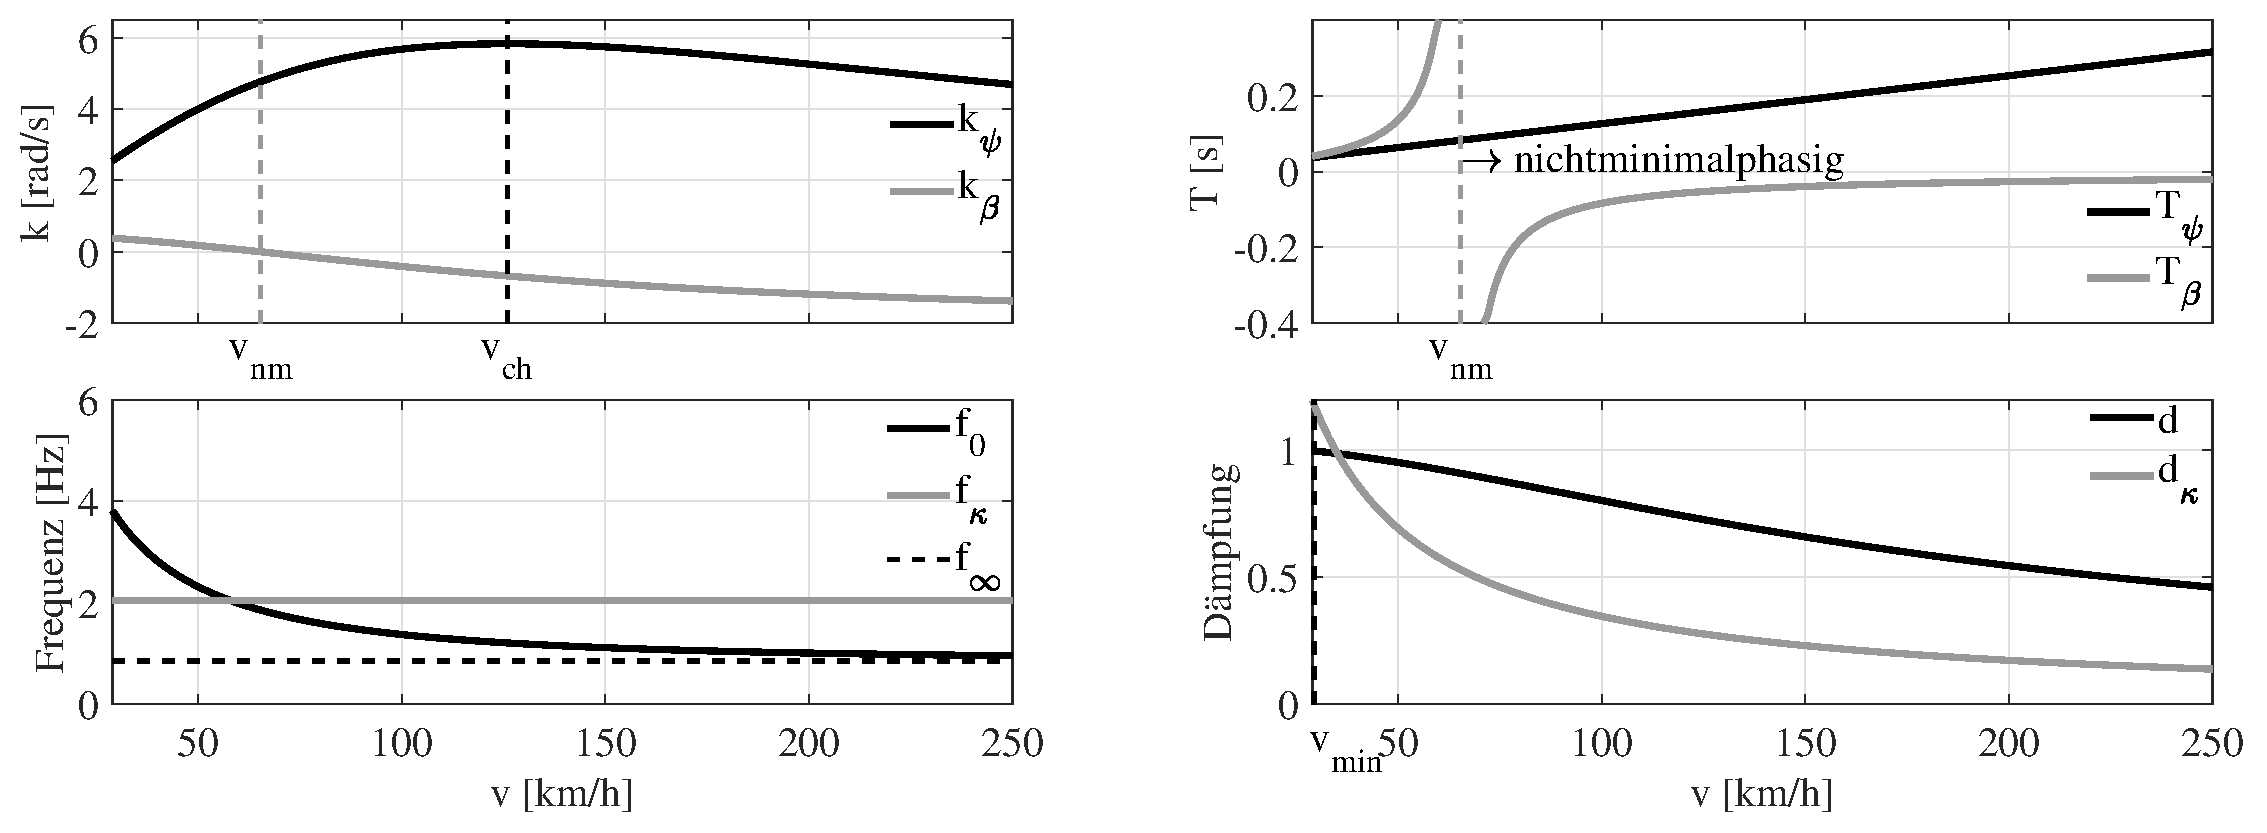
\includegraphics[width=12cm]{Bilder/ESM/esm_erg.eps} 
%	   \includegraphics[scale=1]{Bilder/ESM/esm.eps} 
%		\input{Bilder/ESM/esm.tex}
      \begin{center}
       \caption{Kenngrößen des dynamischen Übertragungsverhaltens}
     		 \label{fig:esm}
       \end{center}
\end{figure}      
Der Grenzwert $\omega_\infty=\lim_{v\to\infty} \omega(v)= (c_r \ell_r -c_f \ell_v)/i_z=2\pi f_\infty$ beschreibt die Bandbreite der Quer- und Gierdynamik für hohe Fahrgeschwindigkeiten. 
%Für große Geschwindigkeiten ist also die Schwerpunktlage, die über Reifen und Achskinematik definierte Balance  als Verhältnis der %Schräglaufsteifigkeiten und das Gierträgheitsmoment für die Bandbreite der Quer- und Gierdynamik bestimmend.  
Es ist leicht zu sehen, daß der Grenzwert der Bandbreite $\lim_{v\to 0} \omega(v)$ gegen $\infty$ geht. Weiterhin wird für $v=v_{\rm lim}$ die Dämpfung $d=1$ (aperiodischer Grenzfall), d.~h. für $v<v_{\rm lim}$ (ca. 20-30km/h) werden die Pole der Übertragungsfunktionen reell und der langsamere Pol der näher am Ursprung liegt wäre dominant und würde das Übertragungsverhalten dominieren. In Fahrversuchen hat sich jedoch gezeigt, dass für niedrige Geschwindigkeiten $v<v_{\rm lim}$ nichtmodellierte Dynamiken eine größere Rolle spielen und    
das vereinfachte lineare Einspurmodell 2. Ordnung nicht geeignet ist, diese Effekte abzubilden. Entsprechende Erweiterungen oder Vereinfachungen müssen für den Niedriggeschwindigkeitsbereich vorgenommen werden, auf die jedoch an dieser Stelle nicht weiter eingegangen werden soll.
Weitere Kenngrößen sind die charakteristische Fahrgeschwindigkeit die sehr gut das stationäre Gierübertragungsverhalten beschreibt. Für $v=v_{ch}$ wird die stationäre Gierverstärkung maximal, d.~h. die Gierempfindlichkeit des Fahrzeugs für diese Fahrgeschwindigkeit ist maximal. Die Geschwindigkeit $v_{nm}$ beschreibt die Fahrgeschwindigkeit oberhalb derer das Schwimmwinkelübertragungsverhalten nichtminimalphasig wird, d.~h. die Nullstellen dieser Übertragungsfunktion wandern im Eigenwertbereich in die rechte Halbebene. Während des Übergangs wechselt gleichzeitig die Schwimmwinkelverstärkung ihr Vorzeichen. Die langsamen Nullstellen haben wegen der geringen Verstärkung in diesem Geschwindigkeitsbereich $v\approx v_{nm}$ keinen bzw. wenig Einfluss auf das Übertragungsverhalten.    

Die Fahrzeugparameter und charakteristischen Kenngrößen des Einspurmodells und damit das Übertragungsverhalten hängen wesentlich von der Fahrzeuggeschwindigkeit, der Fahrzeugbeladung und dem reibwertabhängigen Reifen-Fahrbahnkontakt und damit vom Straßenzustand und der Bereifung ab.
Zusatzbeladung, Reifen und witterungsbedingter Reibwert bewirken Änderungen der Größen $m = m(m_{zus})$, $i_z(m_{zus})$, $l_f(m_{zus})$, $l_r(m_{zus})$, $c_f(m_{zus},\mu)$, $c_r(m_{zus},\mu)$. Für den regelungstechnischen Entwurf ist es notwendig, sich an die mess-, schätz- oder beobachtbaren variierenden Parameter zu adaptieren und entsprechend robust gegenüber nicht mess-, schätz- oder beobachtbaren variierenden Parametern zu sein. Eine Adaption der Reglerfunktionen an die Fahrgeschwindigkeit - ein variierender aber bekannter Parameter des Einspurmodells und gleichzeitig ein beobachteter Fahrzustand - über klassisches \textit{gainscheduling} ist Standard. Eine Adaption an eine veränderliche Zusatzbeladung mit ihrem Einfluss auf mehrere Fahrzeugparameter ist deutlich schwieriger. Das wird dann häufiger erst durch robuste Regleransätze beherrscht. 
Mit dem Betriebsbereich definiert durch die beladungsabhängige Schwerpunktlage, Masse und die variierende Fahrgeschwindigkeit $v\in[v^-, v^+]$, $R_1: m_{R1}$... ................. 

Die Identifikation des Einspurmodells erfolgt im Fahrversuch anhand von bidirektionalen Lenkwinkelsprüngen mit konstanter Querbeschleunigung über den gesamten Geschwindigkeitsbereich. Dieser Vorgang wiederholt für unterschiedliche Zusatzbeladungen und Bereifungen kann als Grundlage für die Bedatung der Parameter des Einspurmodells und für eine Beschreibung der zu betrachtenden Unsicherheiten dienen. 
\begin{figure}[thpb]
 	 \centering
	   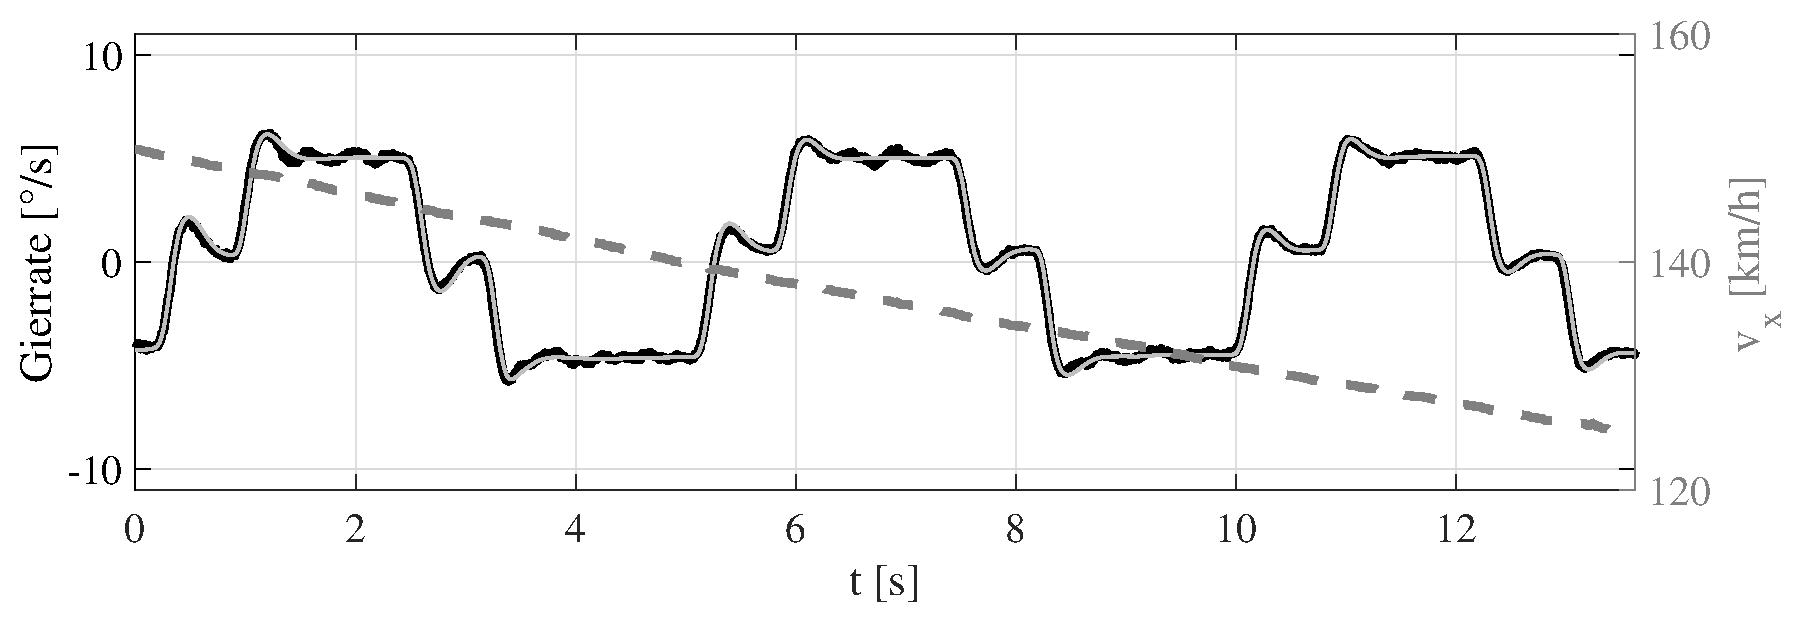
\includegraphics[width=12cm]{Bilder/ESM/esm_bidi_erg.eps} 
      \begin{center}
       \caption{Vergleich zwischen Einspurmodell- und gemessener Gierrate bei bidirektionalen Lenkwinkelsprüngen bei Fahrzeuggeschwindigkeiten zwischen 150 und 120 km/h}
     		 \label{abb_ident_esm}
       \end{center}
\end{figure}      


\subsection{Längsdynamik}
Zur Ansteuerung des Antriebs und der Bremse hat sich in heutigen Fahrzeug-Architekturen die Schnittstelle der Summen-Radmomente durchgesetzt.  Dies ist für die meisten Fahrerassistenzfunktionen ausreichend da keine Einzelradmomente zur Stabilisierung gestellt werden müssen und bietet den Vorteil, dass da so beide Aktuatoren, Antrieb und Bremse,  über die gleiche physikalische Größe angesteuert werden können.  Im Verlauf des Kapitels wird das Übertragungsverhalten vom Sollantriebsmoment $\tau_\mathrm{mot,d}$ bzw. Sollbremsmoment $\tau_\mathrm{brk,d}$ zum gemessen Radmoment $\tau_{xd}$ als System zweiter Ordnung mit Totzeit modelliert:
\begin{equation}
G_{\tau_x}^*(s)=\underbrace{\frac{k\omega_0^2}{s^2+2D\omega_0 s + \omega_0^2}}_{\displaystyle{G_{\tau_x}}}\;\mathrm{e}^{-T_\mathrm{D}s}\label{eq:GLong}
\end{equation}
Wie beim Lenkungsmodell 2 erfolgt die Identifikation im Fahrversuch anhand von Sollradmomentensprüngen bei verschiedenen Fahrzeuggeschwindigkeiten.  Abb.  \ref{abb_ident_antrieb_bremse} veranschaulicht die gute Übereinstimmung zwischen gemessenem und modelliertem Verhalten.
   \begin{figure}[thpb]
      \centering
	\setlength\figureheight{7cm} 
	\setlength\figurewidth{10.5cm}
    % This file was created by matlab2tikz v0.5.0 running on MATLAB 7.11.1.
%Copyright (c) 2008--2014, Nico Schlömer <nico.schloemer@gmail.com>
%All rights reserved.
%Minimal pgfplots version: 1.3
%
%The latest updates can be retrieved from
%  http://www.mathworks.com/matlabcentral/fileexchange/22022-matlab2tikz
%where you can also make suggestions and rate matlab2tikz.
%
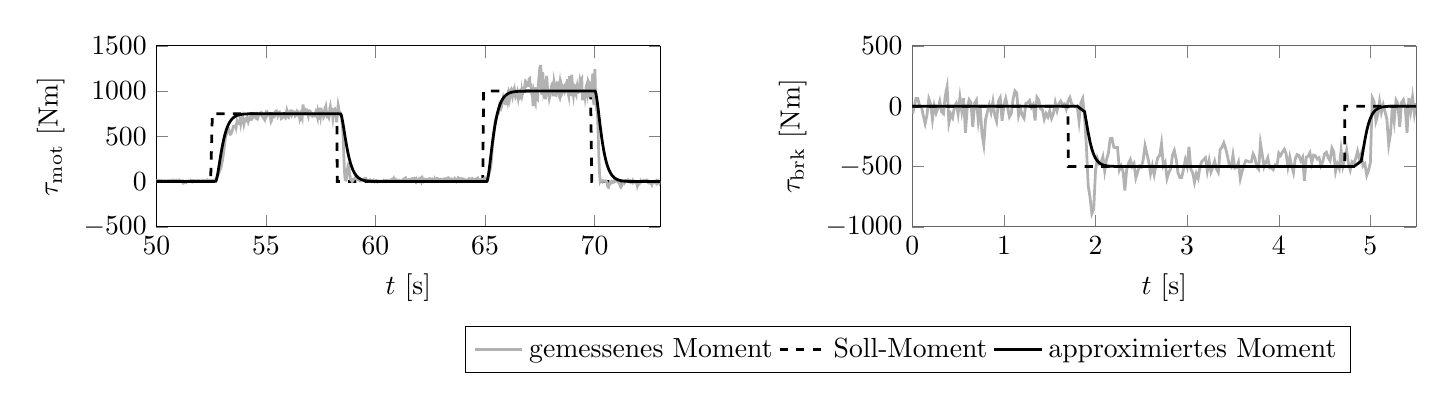
\begin{tikzpicture}



\begin{axis}[%
 /pgf/number format/.cd,
        use comma,
        1000 sep={},
width=0.4\figurewidth,
height=0.383142\figureheight,
at={(0.010779\figurewidth,0\figureheight)},
scale only axis,
separate axis lines,
every outer x axis line/.append style={black},
every x tick label/.append style={font=\color{black}},
xmin=50,
xmax=73,
xlabel={$t$ [s]},
every outer y axis line/.append style={black},
every y tick label/.append style={font=\color{black}},
ymin=-500,
ymax=1500,
ylabel={$\tau_\mathrm{mot}$ [Nm]},
ylabel near ticks
]
\addplot [color=black , dashed, line width=1.0]
  table[row sep=crcr]{%
27.975	0\\
28.395	0\\
28.515	0\\
28.516	200\\
28.735	200\\
37.415	200\\
37.475	500\\
45.195	500\\
45.415	500\\
45.435	0\\
45.535	0\\
52.475	0\\
52.555	750\\
52.655	750\\
58.235	750\\
58.255	0\\
58.355	0\\
64.675	0\\
64.795	0\\
64.895	0\\
64.935	1000\\
69.815	1000\\
69.875	0\\
72.975	0\\
};


\addplot [color=light-gray,solid,line width=1.0]
  table[row sep=crcr]{%
27.975	-14.9009689478901\\
27.995	-8.62108796826086\\
28.015	-3.59000534065733\\
28.035	-6.83712520027438\\
28.055	-7.36166933699522\\
28.075	-4.51262684061924\\
28.095	-13.1582665751122\\
28.115	-10.2533150225068\\
28.135	-6.36714732585603\\
28.155	-0.472037842373989\\
28.175	-5.06512550545481\\
28.195	-0.502677958342659\\
28.215	-1.93250934615062\\
28.235	2.46086823834618\\
28.255	7.71827267872149\\
28.275	9.10684367132084\\
28.295	5.73459983215099\\
28.315	0.29079118028554\\
28.335	-2.60085450522602\\
28.355	-3.08279545281128\\
28.375	-0.943358510719309\\
28.395	6.65319295033199\\
28.415	9.92826733806377\\
28.435	-0.389517051956769\\
28.455	2.13334859235542\\
28.475	6.15928892957982\\
28.495	8.25612268253621\\
28.515	7.91663996337854\\
28.535	8.11500724803559\\
28.555	8.31337453269264\\
28.575	3.39679560540197\\
28.595	-0.261707484550028\\
28.615	-3.16665903715547\\
28.635	0.70351720454746\\
28.655	5.45102616922278\\
28.675	5.32321660181604\\
28.695	2.00688181887565\\
28.715	4.62825970855288\\
28.735	10.4528114747846\\
28.755	2.91485465781671\\
28.775	6.76903944457182\\
28.795	4.45918974593753\\
28.815	0.378683146410641\\
28.835	7.36414129854297\\
28.855	9.10684367132084\\
28.875	10.4528114747846\\
28.895	14.6185244525827\\
28.915	26.3221942473486\\
28.935	40.2079041733421\\
28.955	45.2522926680395\\
28.975	57.0878004119931\\
28.995	79.2996871900507\\
29.015	80.1224536507206\\
29.035	97.6387121385513\\
29.055	104.781277180132\\
29.075	103.392706187533\\
29.095	116.683314259555\\
29.115	127.015747310596\\
29.135	125.159884031433\\
29.155	144.334981307697\\
29.175	150.443106736857\\
29.195	151.249881742579\\
29.215	149.066498817425\\
29.235	153.234897383077\\
29.255	165.026459143968\\
29.275	168.172381170366\\
29.295	174.593377584496\\
29.315	167.918104829479\\
29.335	156.167803463797\\
29.355	162.829770351719\\
29.375	157.898542763408\\
29.395	165.749370565346\\
29.415	172.083817807277\\
29.435	167.818249790187\\
29.455	164.672327763789\\
29.475	173.203463797969\\
29.495	179.849439230944\\
29.515	172.890592812999\\
29.535	170.86565957122\\
29.555	175.11657892729\\
29.575	171.388860914014\\
29.595	164.147783627068\\
29.615	157.600320439459\\
29.635	160.647730220492\\
29.655	164.516563668268\\
29.675	168.470603494315\\
29.695	165.565651941709\\
29.715	167.534676127259\\
29.735	168.641016250857\\
29.755	173.204806591896\\
29.775	175.031372549018\\
29.795	192.05238422217\\
29.815	196.051712825207\\
29.835	173.857160296024\\
29.855	183.650400549324\\
29.875	194.093308918897\\
29.895	186.354299229418\\
29.915	194.786923018233\\
29.935	185.164095521476\\
29.955	180.85592431525\\
29.975	205.898176546882\\
29.995	202.836118104828\\
30.015	199.221560997939\\
30.035	206.989868009459\\
30.055	195.68158999008\\
30.075	198.430777447164\\
30.095	205.345677882046\\
30.115	202.22905317769\\
30.135	230.261463340198\\
30.155	216.696559090561\\
30.175	200.044327458608\\
30.195	224.322407873654\\
30.215	202.49663538567\\
30.235	196.754604409856\\
30.255	199.30676737621\\
30.275	173.641458762492\\
30.295	170.610040436407\\
30.315	185.222690165559\\
30.335	179.071961547264\\
30.355	173.813214312961\\
30.375	170.398367284656\\
30.395	176.123064011596\\
30.415	169.093659876401\\
30.435	177.879072251467\\
30.455	190.802243076217\\
30.475	182.328358892194\\
30.495	211.961013199052\\
30.515	220.080766002897\\
30.535	185.17740138857\\
30.555	213.550637064163\\
30.575	231.350469214922\\
30.595	221.912703135727\\
30.615	221.004730296786\\
30.635	208.689967193101\\
30.655	210.616388189515\\
30.675	200.044327458608\\
30.695	181.2952620737\\
30.715	207.823254749369\\
30.735	211.493720912488\\
30.755	205.867536430913\\
30.775	203.897169451437\\
30.795	201.206576638436\\
30.815	223.298588540473\\
30.835	223.089600976576\\
30.855	198.758297093155\\
30.875	209.155916685739\\
30.895	211.650827801936\\
30.915	198.131212329288\\
30.935	192.461081864651\\
30.955	208.60476081483\\
30.975	206.678339818416\\
30.995	184.937773708704\\
31.015	202.340871290149\\
31.035	206.183093003737\\
31.055	207.626230258639\\
31.075	224.093400473028\\
31.095	204.950286106659\\
31.115	194.121263447012\\
31.135	207.598275730524\\
31.155	199.406622415502\\
31.175	198.99389639124\\
31.195	203.147646295871\\
31.215	202.014694438085\\
31.235	194.502006561378\\
31.255	201.134676127259\\
31.275	204.947600518805\\
31.295	210.672297245745\\
31.315	211.15423819333\\
31.335	204.196734569313\\
31.355	209.185214007781\\
31.375	213.947371633477\\
31.395	205.145967803462\\
31.415	204.478965438314\\
31.435	206.334828717478\\
31.455	197.888899061569\\
31.475	198.613153276873\\
31.495	203.331364919507\\
31.515	208.361104753184\\
31.535	199.533089188981\\
31.555	203.304753185319\\
31.575	213.308323796443\\
31.595	207.90846112764\\
31.615	205.840924696725\\
31.635	202.551201647973\\
31.655	187.302189669641\\
31.675	184.001846341648\\
31.695	191.852674143586\\
31.715	203.047791256579\\
31.735	195.36871900511\\
31.755	204.521568627449\\
31.775	202.5525444419\\
31.795	203.742748149842\\
31.815	214.654291599907\\
31.835	215.406500343326\\
31.855	215.548958571754\\
31.875	202.837460898755\\
31.895	192.208148317691\\
31.915	200.128191042953\\
31.935	203.657541771571\\
31.955	187.388738841839\\
31.975	186.990661478598\\
31.995	198.075303273059\\
32.015	204.509605554283\\
32.035	218.057175555045\\
32.055	224.080094605934\\
32.075	216.442282749674\\
32.095	225.612466620888\\
32.115	225.372838941022\\
32.135	209.343663691156\\
32.155	204.947600518805\\
32.175	197.77708094911\\
32.195	192.462424658578\\
32.215	188.534996566719\\
32.235	193.681925688562\\
32.255	196.432455939573\\
32.275	205.786358434423\\
32.295	207.853894865338\\
32.315	213.763653009841\\
32.335	220.309773403523\\
32.355	212.544151979857\\
32.375	209.386266880292\\
32.395	201.277134355686\\
32.415	193.413000686655\\
32.435	197.098115510794\\
32.455	188.977019913022\\
32.475	194.149217975126\\
32.495	205.176607919431\\
32.535	207.061768520636\\
32.555	218.909239337757\\
32.575	214.614373998625\\
32.595	210.773495078964\\
32.615	215.351934081024\\
32.635	211.339299610893\\
32.655	219.17547875181\\
32.675	216.042862592506\\
32.695	214.940550850689\\
32.715	213.707743953611\\
32.735	203.886549172197\\
32.755	204.324544136719\\
32.775	216.796414129853\\
32.795	214.401358052947\\
32.815	218.015915159837\\
32.835	224.038834210725\\
32.875	222.381338216219\\
32.895	215.406500343326\\
32.915	208.406393530173\\
32.935	204.296589608605\\
32.955	193.934859235522\\
32.975	201.334386205843\\
32.995	213.494728007933\\
33.015	212.17402914473\\
33.035	205.018158236056\\
33.055	218.666926070037\\
33.075	225.199740596626\\
33.095	209.921431296252\\
33.115	221.248386358433\\
33.135	215.734019989317\\
33.155	195.254215304798\\
33.175	206.622430762187\\
33.215	198.75158312352\\
33.235	207.144289311054\\
33.255	208.588769359882\\
33.275	205.639871824214\\
33.295	213.606546120392\\
33.315	221.969954985884\\
33.335	208.008316166932\\
33.355	210.416678110931\\
33.375	225.230380712595\\
33.395	205.344335088119\\
33.415	209.623208972303\\
33.435	217.350255588615\\
33.455	200.582177462423\\
33.475	195.975783932248\\
33.495	209.102693217363\\
33.515	209.454139009688\\
33.535	210.472587167161\\
33.555	212.401693751429\\
33.575	214.865964751658\\
33.595	216.68191042954\\
33.615	212.614709697107\\
33.635	204.665369649804\\
33.655	194.587212939649\\
33.675	202.071946288241\\
33.695	205.658548867016\\
33.715	196.487022201875\\
33.735	202.864072632943\\
33.755	209.030792706186\\
33.775	210.616388189515\\
33.795	211.35126268406\\
33.815	222.081773098343\\
33.835	224.661890592811\\
33.855	211.875806820781\\
33.875	202.893369954984\\
33.895	207.31738765545\\
33.915	219.942336156251\\
33.935	201.900190737772\\
33.955	205.205905241473\\
33.975	197.394995040816\\
33.995	203.488471808956\\
34.015	218.115770199129\\
34.035	209.783001449606\\
34.055	215.77796597238\\
34.075	240.40749217975\\
34.095	232.641870756083\\
34.115	230.602288853283\\
34.135	235.717235065231\\
34.155	219.914381628136\\
34.175	218.002609292743\\
34.195	202.894712748911\\
34.215	206.491935606926\\
34.235	209.837567711908\\
34.255	194.517998016326\\
34.275	203.475165941862\\
34.295	213.381567101547\\
34.315	213.74900434882\\
34.335	219.247379262988\\
34.355	222.495841916532\\
34.375	214.517204547187\\
34.395	212.190020599678\\
34.415	203.31940184634\\
34.435	193.00161745632\\
34.455	212.090165560386\\
34.475	205.757061112381\\
34.495	192.292011902036\\
34.515	209.171908140687\\
34.535	208.619409475851\\
34.555	204.564171816585\\
34.575	232.442160677499\\
34.595	221.871442740519\\
34.615	222.182970931562\\
34.635	227.624093995573\\
34.655	202.371511406118\\
34.675	217.805584802013\\
34.695	226.887876707101\\
34.715	211.540352483404\\
34.735	223.699351491568\\
34.755	221.004730296786\\
34.775	226.786678873882\\
34.795	223.741954680703\\
34.815	208.832425421529\\
34.835	214.473258564125\\
34.855	214.277576867321\\
34.875	210.17973601892\\
34.895	209.625894560157\\
34.915	205.473487449453\\
34.935	207.088380254824\\
34.955	200.245380331119\\
34.975	194.420828564888\\
34.995	201.744426642251\\
35.015	206.763546196687\\
35.035	202.866758220797\\
35.055	208.944243533988\\
35.075	215.77796597238\\
35.095	212.348470283053\\
35.115	205.445532921338\\
35.135	207.289433127335\\
35.155	212.659998474096\\
35.175	218.965148393986\\
35.195	211.992996108948\\
35.215	212.120805676355\\
35.235	217.802899214159\\
35.255	218.895933470663\\
35.275	214.983154039825\\
35.295	227.058289463644\\
35.315	221.079316395818\\
35.335	220.31111619745\\
35.355	223.642099641411\\
35.375	211.087708857861\\
35.395	207.330693522544\\
35.415	207.684824902722\\
35.435	198.489372091248\\
35.455	198.899412527656\\
35.475	204.184771496146\\
35.495	204.284626535438\\
35.515	205.446875715265\\
35.535	205.106050202181\\
35.555	202.937315938047\\
35.575	209.953414206148\\
35.595	210.223682001982\\
35.615	219.464423590446\\
35.635	217.692423895627\\
35.655	199.09912260624\\
35.675	205.828961623559\\
35.695	210.279591058212\\
35.715	208.366475928892\\
35.735	207.626230258639\\
35.755	205.16195925841\\
35.775	213.396215762568\\
35.795	221.119233997099\\
35.815	218.794735637444\\
35.835	227.287296864269\\
35.855	218.286182955671\\
35.875	207.073731593803\\
35.895	203.263492790111\\
35.915	207.445197222857\\
35.935	190.251087205309\\
35.955	189.472266727701\\
35.975	201.334386205843\\
35.995	193.154695963987\\
36.015	201.98673990997\\
36.035	224.707179369801\\
36.055	217.801556420232\\
36.075	223.840466926068\\
36.095	220.413656824596\\
36.115	220.934172579536\\
36.135	227.083558403905\\
36.155	215.055054551002\\
36.175	216.343770504309\\
36.195	219.03436331731\\
36.215	204.341878385594\\
36.235	211.640207522696\\
36.255	222.352040894177\\
36.275	224.536766613259\\
36.295	223.982925154496\\
36.315	220.976775768672\\
36.335	226.533745326923\\
36.355	215.904432745859\\
36.375	201.349034866864\\
36.395	219.958327611199\\
36.415	216.79775692378\\
36.435	209.414221408406\\
36.455	216.767116807811\\
36.475	213.919417105362\\
36.495	212.02229343099\\
36.515	207.285404745554\\
36.535	213.947371633477\\
36.555	226.577691309985\\
36.575	219.292668039977\\
36.595	212.674647135117\\
36.615	220.35640497444\\
36.635	214.952513923856\\
36.655	209.7963073167\\
36.675	204.227374685281\\
36.695	205.755718318454\\
36.715	210.844052796214\\
36.735	211.384588387883\\
36.755	219.630807965208\\
36.775	227.168764782176\\
36.795	229.6650186923\\
36.815	231.394415197984\\
36.835	225.866742961774\\
36.855	218.965148393986\\
36.875	216.427634088653\\
36.895	218.865293354694\\
36.915	210.915953307391\\
36.935	215.917738612953\\
36.955	217.532631418324\\
36.975	210.37676050965\\
36.995	208.391744869152\\
37.015	212.940886549171\\
37.035	218.270191500723\\
37.055	227.327214465551\\
37.075	220.142046234835\\
37.095	214.573113603417\\
37.115	219.491035324634\\
37.135	217.62052338445\\
37.155	213.382909895474\\
37.175	211.710765239947\\
37.195	213.368261234453\\
37.215	217.293003738459\\
37.235	219.278019378956\\
37.255	225.656412603951\\
37.295	219.577584496832\\
37.315	210.846738384068\\
37.335	201.238559548332\\
37.355	197.850324254214\\
37.375	206.014023041122\\
37.395	200.38649576562\\
37.415	206.168444342716\\
37.435	206.534538796062\\
37.455	207.27209887846\\
37.475	211.325993743799\\
37.495	213.791607537955\\
37.515	219.29132524605\\
37.535	222.694209201189\\
37.555	217.917402914472\\
37.575	210.645685511557\\
37.595	196.516319523917\\
37.615	191.979140917066\\
37.635	195.991775387196\\
37.655	205.614602883954\\
37.675	205.201876859692\\
37.695	206.903318837261\\
37.715	215.507698176545\\
37.735	224.974761577781\\
37.755	253.928450446325\\
37.775	278.756343938351\\
37.795	288.705348287173\\
37.815	288.038345922024\\
37.835	289.187289234758\\
37.855	300.978850995649\\
37.875	306.575738155182\\
37.895	299.218814373996\\
37.915	302.47789730678\\
37.935	305.412146181427\\
37.955	306.702204928662\\
37.975	309.637796597236\\
37.995	316.808316166931\\
38.015	327.665293354694\\
38.035	347.096009765771\\
38.055	350.353749904628\\
38.075	348.158403906307\\
38.095	344.089860379947\\
38.115	339.579293507283\\
38.135	350.890257114516\\
38.155	354.237232013425\\
38.175	363.037293049513\\
38.195	381.689188982983\\
38.215	382.228381780725\\
38.235	398.708857862208\\
38.255	415.886976424808\\
38.275	408.572655832758\\
38.295	400.663233386737\\
38.315	394.358083466847\\
38.335	408.328999771111\\
38.355	410.866514076444\\
38.375	408.810940718697\\
38.395	425.148958571752\\
38.415	438.018905928126\\
38.435	432.320820935375\\
38.455	442.836972610052\\
38.475	458.752986953533\\
38.495	466.461356527043\\
38.515	475.674143587392\\
38.535	474.201709010449\\
38.555	474.526543068586\\
38.575	468.984222171355\\
38.595	470.330189974819\\
38.615	477.585915922785\\
38.635	481.087312123289\\
38.655	479.783947508961\\
38.675	474.199023422595\\
38.695	479.967666132597\\
38.715	481.55594720378\\
38.735	479.175539787896\\
38.755	476.9628595407\\
38.775	463.029175249863\\
38.795	453.267917906459\\
38.815	469.19858091096\\
38.835	488.4269016556\\
38.855	473.402868696113\\
38.875	468.129472800789\\
38.895	466.995178149077\\
38.915	473.259067673758\\
38.935	480.501487754631\\
38.955	479.553597314408\\
38.975	489.574502174407\\
38.995	490.736751354234\\
39.015	487.762584878305\\
39.035	490.454520485233\\
39.055	497.085847257187\\
39.075	494.520378423739\\
39.095	491.630075532154\\
39.115	493.499244678412\\
39.135	480.28981460288\\
39.155	490.324025329972\\
39.175	502.967650873575\\
39.195	496.095353627828\\
39.215	495.911635004192\\
39.235	497.554482337678\\
39.255	503.205935759514\\
39.275	507.797680628667\\
39.295	498.076340886545\\
39.315	505.17630273899\\
39.335	507.233218890665\\
39.355	519.959365224685\\
39.375	520.752834363313\\
39.395	500.476768139158\\
39.415	518.998168917368\\
39.435	502.47508964675\\
39.455	500.150591287095\\
39.475	509.094453345537\\
39.495	501.625711451892\\
39.515	506.314625772484\\
39.535	505.406652933543\\
39.555	501.194308384828\\
39.575	505.093781948573\\
39.595	520.242938887613\\
39.615	525.854474708167\\
39.635	518.004989700156\\
39.655	509.443213550007\\
39.675	501.423315785454\\
39.695	512.081925688559\\
39.715	508.906706340119\\
39.735	513.909834439608\\
39.755	518.586785687033\\
39.775	514.307911802849\\
39.795	514.535576409548\\
39.815	518.122178988323\\
39.835	525.90244907301\\
39.855	521.877851529713\\
39.875	526.638666361482\\
39.895	520.161760891123\\
39.915	512.478660257873\\
39.935	507.984084840158\\
39.955	506.795223926142\\
39.975	517.365941863122\\
39.995	517.138277256424\\
40.015	522.724544136717\\
40.035	520.442648966197\\
40.055	521.507728694587\\
40.075	526.227283131147\\
40.095	521.419836728461\\
40.115	526.906248569462\\
40.135	524.552452887766\\
40.155	502.444449530781\\
40.175	519.208499275192\\
40.195	526.192614633398\\
40.215	519.520027466235\\
40.235	527.368169680319\\
40.255	518.753170061795\\
40.275	527.248416876474\\
40.295	529.14419775692\\
40.315	524.352742809182\\
40.335	515.78168917372\\
40.355	513.770061799035\\
40.375	517.781353475238\\
40.395	521.662149996181\\
40.415	528.734157320511\\
40.435	529.216098268097\\
40.455	523.078675516895\\
40.475	524.953215838861\\
40.495	514.381155107954\\
40.515	526.309803921564\\
40.535	523.150576028072\\
40.555	507.150698100248\\
40.575	509.375341420611\\
40.595	515.143984130613\\
40.615	527.827527275497\\
40.635	523.022766460666\\
40.655	517.242160677496\\
40.675	519.894178683142\\
40.695	519.767711909663\\
40.715	506.644831006329\\
40.735	509.436621652548\\
40.755	518.775875486377\\
40.775	512.073990997173\\
40.795	514.029709315629\\
40.815	518.706660563054\\
40.835	521.624917982753\\
40.855	524.174395361253\\
40.875	527.179201953151\\
40.895	543.602426184477\\
40.915	537.989547569996\\
40.935	530.207934691382\\
40.955	518.798458838784\\
40.975	510.115587090864\\
40.995	516.904020752266\\
41.015	536.377340352479\\
41.035	540.572350652319\\
41.055	550.886106660559\\
41.075	545.99882505531\\
41.095	537.496986343171\\
41.115	529.956343938349\\
41.135	526.785152971691\\
41.155	527.067383840692\\
41.175	524.925261310746\\
41.195	517.725444419009\\
41.215	523.207827878229\\
41.235	523.054749370561\\
41.255	523.705760280762\\
41.275	522.245288776985\\
41.295	535.041992828256\\
41.315	538.456839856561\\
41.335	542.014145113294\\
41.355	541.68796826123\\
41.375	523.660471503772\\
41.395	518.403067063397\\
41.415	513.908491645681\\
41.435	518.171374074917\\
41.455	527.228397039745\\
41.475	520.582421606771\\
41.495	517.324681467914\\
41.515	521.391882200347\\
41.535	518.340444037533\\
41.555	509.56833752956\\
41.575	503.826306553746\\
41.595	504.153826199736\\
41.615	519.87147325856\\
41.635	522.523491264206\\
41.655	522.739192797737\\
41.675	530.858945601583\\
41.695	544.618188754096\\
41.715	539.700267032879\\
41.735	528.913847562367\\
41.755	524.307454032192\\
41.775	520.88064393072\\
41.795	520.272236209655\\
41.815	517.123628595403\\
41.835	513.240146486606\\
41.855	522.619317921717\\
41.875	517.942366674292\\
41.895	518.213977264053\\
41.915	520.651636530094\\
41.935	515.098695353624\\
41.955	500.869474326691\\
41.975	502.50035858701\\
41.995	513.11636530098\\
42.015	509.074433508808\\
42.035	514.049607080182\\
42.055	522.542168307007\\
42.075	529.615518425265\\
42.095	526.002304112302\\
42.115	517.396581979091\\
42.135	503.733165484088\\
42.175	500.106645304032\\
42.195	494.987670710303\\
42.215	489.75956359197\\
42.235	513.919111924921\\
42.255	519.176516365296\\
42.275	510.65868619821\\
42.295	523.994583047222\\
42.315	526.09947356374\\
42.335	499.752513923853\\
42.355	493.798809796288\\
42.375	504.26173800259\\
42.395	499.185366597997\\
42.415	524.133134966045\\
42.435	531.970656900889\\
42.455	533.96897840848\\
42.475	515.20526436255\\
42.495	502.29271381704\\
42.515	502.021103227279\\
42.535	489.919356069272\\
42.555	501.467261768517\\
42.575	504.71169604028\\
42.595	514.547539482715\\
42.615	525.260715648123\\
42.635	534.275135423815\\
42.655	530.351735713737\\
42.675	531.017395284958\\
42.695	515.102723735404\\
42.715	509.304783703361\\
42.735	501.77878995956\\
42.755	502.544304570073\\
42.775	507.575387197677\\
42.795	511.741100175475\\
42.815	522.34380102235\\
42.835	523.238467994197\\
42.855	525.37790493629\\
42.875	520.091203173872\\
42.895	511.745128557256\\
42.915	487.509651331346\\
42.935	488.384298466464\\
42.955	500.221149004345\\
42.975	507.177309834435\\
42.995	512.495994506748\\
43.015	526.216662851907\\
43.035	510.010360875864\\
43.055	505.663614862283\\
43.075	496.406881818871\\
43.095	492.933440146483\\
43.115	502.529655909052\\
43.135	508.279621576253\\
43.155	513.047150377657\\
43.175	516.109208819711\\
43.195	527.073975738151\\
43.215	511.418951705192\\
43.235	508.613855191878\\
43.255	509.280857557027\\
43.275	494.388662546727\\
43.295	490.236255436023\\
43.315	499.942946517124\\
43.335	502.874509803918\\
43.355	514.153490501255\\
43.375	511.277836270691\\
43.395	509.263523308152\\
43.415	511.317753871973\\
43.435	496.934111543446\\
43.455	500.545983062482\\
43.475	512.902006561375\\
43.495	507.562081330583\\
43.515	500.942717631796\\
43.535	504.257709620809\\
43.555	508.665735866327\\
43.575	507.756420233459\\
43.595	504.027359426256\\
43.615	491.4862745098\\
43.635	494.391226062405\\
43.655	507.515449759666\\
43.675	520.169695582509\\
43.695	527.878065156019\\
43.715	519.802258335236\\
43.735	525.670756084531\\
43.755	518.529533836877\\
43.775	511.13269245441\\
43.795	508.764248111692\\
43.815	501.905256733039\\
43.835	505.772747386888\\
43.855	516.263630121305\\
43.875	514.267994201568\\
43.895	520.629053177687\\
43.915	503.562752727546\\
43.935	499.804394598302\\
43.955	482.976501106275\\
43.975	481.557289997707\\
43.995	502.653437094678\\
44.015	504.428122377351\\
44.035	515.133363851373\\
44.055	518.052964065\\
44.075	519.582650492099\\
44.095	514.720637827111\\
44.115	508.356893263138\\
44.135	497.346837567708\\
44.155	491.891065842676\\
44.175	498.435843442431\\
44.195	508.496665903711\\
44.215	522.36504158083\\
44.235	517.843854428927\\
44.255	508.793545433734\\
44.275	503.612069886316\\
44.295	511.461554894327\\
44.315	511.831677729454\\
44.335	510.513664454105\\
44.355	497.754192416262\\
44.375	499.146791790642\\
44.395	499.901686121916\\
44.415	513.901899748222\\
44.435	527.529304951548\\
44.455	520.993804837106\\
44.475	502.873167009991\\
44.495	500.708461127638\\
44.515	503.750499732963\\
44.535	503.49488059815\\
44.555	511.235233081556\\
44.575	525.310032806893\\
44.595	515.431586175322\\
44.615	501.939925230789\\
44.635	495.818493934535\\
44.655	489.397497520405\\
44.675	465.167391470203\\
44.695	463.905287251084\\
44.715	482.622369726097\\
44.735	497.388097962917\\
44.755	505.694254978252\\
44.775	501.44467841611\\
44.795	490.24821850919\\
44.815	472.147478446628\\
44.835	476.727260242615\\
44.855	485.004119935908\\
44.875	475.108339055463\\
44.895	490.999084458682\\
44.915	503.10083161669\\
44.935	508.38619058518\\
44.955	489.607827878229\\
44.975	483.072327763786\\
44.995	486.360708018612\\
45.015	482.322804608221\\
45.035	487.633432516972\\
45.055	504.470725566487\\
45.075	514.037644007015\\
45.095	511.614633401995\\
45.115	506.327931639578\\
45.135	506.501029983974\\
45.155	505.153719386583\\
45.175	517.807965209426\\
45.195	524.282185091931\\
45.215	532.447226672766\\
45.235	525.558937972072\\
45.255	516.75619134813\\
45.275	513.059113450824\\
45.295	515.784374761574\\
45.315	502.391226062406\\
45.335	508.541954680701\\
45.355	514.097581445025\\
45.375	515.130678263519\\
45.395	518.871702143888\\
45.415	516.788174258026\\
45.435	509.139742122526\\
45.455	502.934447241928\\
45.475	495.21008621347\\
45.495	492.205279621573\\
45.515	500.253131914241\\
45.535	494.499137865259\\
45.555	510.938353551533\\
45.575	521.284092469669\\
45.595	507.126771953914\\
45.615	488.094132906077\\
45.635	459.013977264054\\
45.655	422.660761425189\\
45.675	363.335515373462\\
45.695	280.673487449453\\
45.715	198.050034332798\\
45.735	132.021560997939\\
45.755	79.2158236057065\\
45.775	50.4471961547263\\
45.795	54.1589227130539\\
45.815	57.9718471046004\\
45.835	71.0800793469135\\
45.855	95.5831387808036\\
45.875	105.88761730373\\
45.895	112.023697261005\\
45.915	114.036667429617\\
45.935	98.8449073014415\\
45.955	70.6274357213699\\
45.975	55.5754482337679\\
45.995	33.5393453879606\\
46.015	17.2971541924163\\
46.035	14.477409018082\\
46.055	13.6839398794538\\
46.075	12.1542534523539\\
46.095	10.6378728923478\\
46.115	4.51644159609396\\
46.135	13.4855725947968\\
46.155	8.72475776302759\\
46.175	8.44118410009938\\
46.195	14.1938353551538\\
46.215	10.6658274204625\\
46.235	8.52639047837054\\
46.255	8.28542000457791\\
46.275	7.69031815060676\\
46.295	8.04444953078528\\
46.315	8.32802319371349\\
46.355	11.6150606546122\\
46.375	8.37062638284907\\
46.415	3.56720836194429\\
46.435	8.32802319371349\\
46.455	10.8641947051196\\
46.475	8.44118410009938\\
46.495	6.25914396887183\\
46.535	6.93945220111414\\
46.555	8.24281681544233\\
46.575	5.86240939955773\\
46.595	6.14598306248594\\
46.615	4.36067750057249\\
46.635	-1.39197375448196\\
46.655	0.591699092088541\\
46.675	-1.63294422827459\\
46.695	7.53455405508529\\
46.715	7.25098039215708\\
46.735	-2.90835431448805\\
46.755	-17.3931944762336\\
46.775	-9.81263447013013\\
46.795	-12.9585564965282\\
46.815	-13.2141756313417\\
46.835	-16.74352635996\\
46.855	-23.7289845120923\\
46.875	-16.0618753337907\\
46.895	-6.14216830701122\\
46.915	-7.67185473411119\\
46.935	-3.71781490806407\\
46.955	-3.83231860837693\\
46.975	-4.66704814221374\\
46.995	-7.68516060120507\\
47.015	5.77451743343263\\
47.035	-3.79105821316832\\
47.055	1.42642862592535\\
47.075	-5.97041275654193\\
47.095	-1.03918516823041\\
47.115	-4.39946593423335\\
47.135	2.5140917067217\\
47.155	3.83210498207074\\
47.175	-2.14821087968246\\
47.195	-6.69735255970073\\
47.215	-1.29480430304389\\
47.235	1.96562142366704\\
47.255	-3.3490348668647\\
47.295	-11.045441367208\\
47.315	-2.26002899214138\\
47.335	3.12652780956764\\
47.355	5.94627298390192\\
47.375	6.63988708323811\\
47.395	4.50045014114614\\
47.415	1.80985732814557\\
47.435	5.1954070344093\\
47.455	2.14934004730324\\
47.475	4.62825970855288\\
47.495	3.74958419165352\\
47.515	8.66750591287116\\
47.535	1.84977492942721\\
47.555	11.4872510872054\\
47.575	12.1955138475625\\
47.595	8.51174181734969\\
47.615	8.90847638666379\\
47.635	8.45448996719326\\
47.655	13.5414816510263\\
47.675	9.74454871442757\\
47.695	11.8839856565195\\
47.715	15.7235217822538\\
47.735	12.5216906996263\\
47.755	10.0986800946061\\
47.775	12.8052643625545\\
47.795	11.1331197070269\\
47.815	8.24281681544233\\
47.835	6.52806897077919\\
47.855	1.05899137865295\\
47.875	6.4149080643933\\
47.895	17.325108720531\\
47.915	9.70194552529199\\
47.935	8.20021362630675\\
47.955	7.2083772030215\\
47.975	6.06077668421478\\
47.995	7.95924315251412\\
48.015	4.04780651560258\\
48.035	4.2182192721449\\
48.055	-0.531975280384358\\
48.075	-10.747219043259\\
48.095	-4.07194628824259\\
48.115	-21.1342183566028\\
48.135	-25.1748073548481\\
48.155	-43.087800411993\\
48.175	-51.1662928206295\\
48.195	-47.664896620126\\
48.215	-41.6859235522997\\
48.235	-27.3581902800026\\
48.255	-14.8437170977337\\
48.275	-5.53241779201922\\
48.295	2.60332646677377\\
48.315	-0.486686503394839\\
48.335	-7.60263981078785\\
48.355	-4.28630502784746\\
48.375	0.475852597848711\\
48.395	0.220233463035232\\
48.415	6.35765621423687\\
48.435	6.72643625543624\\
48.455	-0.586541542686849\\
48.475	2.48882276646091\\
48.495	6.03147936217308\\
48.515	-2.13221942473464\\
48.535	-0.74364843213529\\
48.555	7.71827267872149\\
48.575	5.84776073853688\\
48.595	5.97557030594362\\
48.615	9.46097505149936\\
48.635	7.23633173113623\\
48.655	2.47551689936703\\
48.675	5.8051575494013\\
48.695	4.27278553444739\\
48.715	1.75126268406217\\
48.735	5.93162432288107\\
48.755	4.33003738460382\\
48.775	-4.05998321507568\\
48.795	-0.24840161745615\\
48.815	5.20871290150318\\
48.835	2.9987182421609\\
48.855	-0.458731975280109\\
48.875	-3.010894941634\\
48.895	-2.06031891355736\\
48.915	2.77239642938912\\
48.935	0.362691691462821\\
48.955	1.01370260166343\\
48.975	6.34032196536208\\
48.995	9.90031280994904\\
49.015	8.38393224994295\\
49.035	4.45650415808359\\
49.055	2.41557946135666\\
49.095	5.63340199893201\\
49.115	4.41390096894801\\
49.135	8.96304264896628\\
49.155	3.63642328526763\\
49.175	5.86106660563076\\
49.195	9.07754634927914\\
49.215	4.65487144274064\\
49.235	2.3596704051272\\
49.255	-3.52079041733399\\
49.275	-1.19629205767885\\
49.295	1.11490043488241\\
49.315	-1.15368886854327\\
49.335	7.32153810940739\\
49.355	6.10203707942339\\
49.375	6.99401846341663\\
49.395	-0.318959334706459\\
49.415	-5.26483558403883\\
49.435	3.35284962233942\\
49.455	-1.84730296787946\\
49.475	0.19093614099353\\
49.495	6.89416342412462\\
49.515	5.52158388647309\\
49.535	-3.30643167772912\\
49.555	1.32791638056031\\
49.575	0.505149919890411\\
49.595	-12.0239719233994\\
49.615	0.80337224383947\\
49.635	5.12484931715899\\
49.655	3.02667277027563\\
49.675	6.34435034714299\\
49.695	2.89886320286889\\
49.715	5.29526207370131\\
49.735	7.67566948958591\\
49.755	8.11500724803559\\
49.775	5.08224612802341\\
49.795	4.03181506065476\\
49.815	6.42687113756021\\
49.835	11.9119401846343\\
49.855	9.3757686732282\\
49.875	6.88220035095771\\
49.895	5.33786526283689\\
49.915	3.90669108110196\\
49.935	7.12317082475034\\
49.955	7.32153810940739\\
49.975	6.64122987716508\\
49.995	9.81510643167788\\
50.015	8.11500724803559\\
50.035	14.4627603570612\\
50.055	15.2136263065538\\
50.075	11.1331197070269\\
50.095	13.2725566491189\\
50.115	13.9102616922256\\
50.135	11.331486991684\\
50.155	10.5380178530558\\
50.175	12.4790875104907\\
50.195	13.7118944075686\\
50.215	9.74454871442757\\
50.235	8.75271229114232\\
50.255	5.18210116731542\\
50.275	8.99368276493495\\
50.295	6.8116426337074\\
50.315	7.36414129854297\\
50.335	4.98373388265837\\
50.355	5.77720302128657\\
50.375	9.50357824063494\\
50.395	11.1757228961625\\
50.415	7.67566948958591\\
50.435	5.18210116731542\\
50.455	4.4312352178228\\
50.475	6.0181734950792\\
50.495	3.39679560540197\\
50.515	5.73459983215099\\
50.535	12.1249561303122\\
50.555	12.3233234149692\\
50.575	7.76087586785707\\
50.595	4.21687647821793\\
50.615	6.72643625543624\\
50.635	9.94291599908462\\
50.655	9.14944686045642\\
50.675	4.4312352178228\\
50.695	6.57067215991477\\
50.715	13.4283207446404\\
50.735	8.15761043717117\\
50.755	9.90031280994904\\
50.775	13.3151598382545\\
50.795	14.3495994506753\\
50.815	16.1349050125887\\
50.835	15.6955672541391\\
50.855	13.3577630273901\\
50.875	12.3659266041048\\
50.895	14.3922026398109\\
50.915	8.7953154802779\\
50.935	5.42307164110805\\
50.955	10.5806210421914\\
50.975	11.5724574654766\\
50.995	11.3740901808196\\
51.015	8.44118410009938\\
51.035	14.5905699244679\\
51.055	7.80347905699265\\
51.075	10.5806210421914\\
51.095	7.2083772030215\\
51.115	7.01000991836445\\
51.135	3.2410315098805\\
51.155	6.96740672922887\\
51.175	4.23286793316575\\
51.195	-3.54605935759478\\
51.215	1.45572594796705\\
51.235	-13.1995269703208\\
51.255	-8.91931029220992\\
51.275	1.18411535820575\\
51.295	1.02835126268428\\
51.315	-6.92233157854554\\
51.335	-3.26651407644748\\
51.355	-6.7945220111388\\
51.375	4.10505836575901\\
51.395	1.92301823453146\\
51.415	4.10505836575901\\
51.435	1.52494087129039\\
51.475	5.73459983215099\\
51.495	1.79386587319775\\
51.515	3.53656824597562\\
51.535	6.52806897077919\\
51.555	13.3151598382545\\
51.575	8.07240405890001\\
51.595	7.87403677424296\\
51.615	9.74454871442757\\
51.635	2.23320363164743\\
51.655	9.57413595788525\\
51.675	11.2462806134128\\
51.695	9.46097505149936\\
51.715	12.0823529411766\\
51.735	11.0479133287558\\
51.755	8.15761043717117\\
51.775	6.32970168612214\\
51.795	5.97557030594362\\
51.815	4.98373388265837\\
51.835	11.6856183718625\\
51.855	12.6774547951477\\
51.875	11.8839856565195\\
51.895	10.2970473792631\\
51.915	11.2462806134128\\
51.935	7.32153810940739\\
51.955	9.65934233615641\\
51.975	5.73459983215099\\
51.995	3.90669108110196\\
52.015	1.01370260166343\\
52.035	3.01336690318175\\
52.055	11.0905165178913\\
52.075	13.7118944075686\\
52.095	8.86587319752821\\
52.115	10.4528114747846\\
52.135	7.71827267872149\\
52.155	6.32970168612214\\
52.175	6.72643625543624\\
52.195	10.9347524223699\\
52.215	9.54618142977052\\
52.235	7.76087586785707\\
52.255	11.7708247501336\\
52.275	11.8839856565195\\
52.295	13.7118944075686\\
52.315	15.497199969482\\
52.335	18.8694438086519\\
52.355	14.9020981155109\\
52.375	13.159395742733\\
52.415	10.6937819485772\\
52.435	7.36414129854297\\
52.455	10.1412832837417\\
52.475	12.1249561303122\\
52.495	14.3495994506753\\
52.515	11.9691920347907\\
52.535	10.7789883268484\\
52.575	11.4166933699551\\
52.595	15.7807736324102\\
52.615	16.3332722972458\\
52.635	15.5398031586176\\
52.655	16.0923018234532\\
52.675	17.126741435874\\
52.695	17.9202105745022\\
52.715	19.7481193255512\\
52.735	41.9719691767757\\
52.755	44.2964675364308\\
52.775	56.5127183947507\\
52.795	64.8454871442738\\
52.815	72.7668726634619\\
52.835	82.7997405966273\\
52.855	94.8881818875404\\
52.875	112.348531319142\\
52.895	132.005569542991\\
52.915	137.7609063859\\
52.935	143.911635004195\\
52.955	162.815121690698\\
52.975	188.339314869915\\
52.995	210.829404135193\\
53.015	230.443839169908\\
53.035	264.47121385519\\
53.055	294.444693675133\\
53.075	334.905027847712\\
53.095	379.887891966122\\
53.115	417.76945143816\\
53.135	455.762829022656\\
53.155	493.290257114515\\
53.175	505.776775768669\\
53.195	522.528862439914\\
53.215	550.136583504993\\
53.235	561.587319752799\\
53.255	562.676325627523\\
53.275	580.051468680853\\
53.295	582.4758220798\\
53.315	566.758175020977\\
53.335	549.653299763481\\
53.355	531.399481193251\\
53.375	523.066712443728\\
53.395	527.501350423434\\
53.415	532.89987029831\\
53.435	541.855695429918\\
53.455	556.594811932551\\
53.475	574.379995422289\\
53.495	593.033234149686\\
53.515	607.629892423891\\
53.535	606.848386358429\\
53.555	603.761058976115\\
53.575	602.002365148389\\
53.595	618.128709849693\\
53.615	620.648889906152\\
53.635	600.708278019374\\
53.655	632.045059891656\\
53.675	660.361043717092\\
53.695	640.57888151369\\
53.715	640.791897459368\\
53.735	646.531242847328\\
53.755	642.621149004344\\
53.775	642.337575341415\\
53.795	653.56198977645\\
53.815	691.142641336685\\
53.835	678.12095826657\\
53.855	640.540306706335\\
53.875	665.910078583958\\
53.895	684.203814755469\\
53.915	672.751735713735\\
53.935	670.075791561756\\
53.955	697.454505226209\\
53.975	668.185259784842\\
53.995	637.430273899438\\
54.015	661.127901121533\\
54.035	687.546761272597\\
54.055	689.987106126492\\
54.075	695.060791943231\\
54.095	691.430243381394\\
54.115	679.853040360108\\
54.135	685.705546654454\\
54.155	705.787273975733\\
54.175	686.285999847404\\
54.195	664.066178377961\\
54.215	680.887479972528\\
54.235	684.572594796668\\
54.255	685.877302204923\\
54.275	709.941023880364\\
54.295	719.67566948958\\
54.315	698.102830548556\\
54.335	686.329945830467\\
54.355	687.988784618901\\
54.375	696.756862745092\\
54.395	721.158724345763\\
54.415	729.7471122301\\
54.435	718.819577325087\\
54.455	718.393545433732\\
54.475	729.05081254291\\
54.495	718.481437399857\\
54.515	723.469916838325\\
54.535	734.223010605014\\
54.555	716.380575265119\\
54.575	697.964400701909\\
54.595	700.046585793845\\
54.615	694.313832303343\\
54.635	706.741756313414\\
54.655	746.66826886396\\
54.675	749.674418249784\\
54.695	736.16810864423\\
54.715	739.581612878608\\
54.735	742.827389944298\\
54.755	754.00785839627\\
54.775	758.981689173718\\
54.795	747.387151903557\\
54.815	726.69835965514\\
54.835	719.483894102382\\
54.855	733.994003204388\\
54.875	724.300617990381\\
54.895	719.416021972986\\
54.915	694.039658197904\\
54.935	686.288685435258\\
54.955	735.828625925072\\
54.975	747.080994888222\\
54.995	723.531197070262\\
55.015	716.642908369568\\
55.035	731.549752040888\\
55.055	744.024307621876\\
55.075	762.676203555346\\
55.095	755.899732967111\\
55.115	738.450003814749\\
55.135	733.900862134731\\
55.155	739.007873655293\\
55.175	733.02755779354\\
55.195	721.888349736776\\
55.215	699.186587319747\\
55.235	665.726359960321\\
55.255	675.31854734111\\
55.275	726.192492561221\\
55.295	750.72619211108\\
55.315	751.154909590289\\
55.335	728.350606546115\\
55.355	713.692668039973\\
55.375	713.326573586627\\
55.395	733.53745326924\\
55.415	766.214831769277\\
55.435	771.333806363006\\
55.455	760.693873502703\\
55.475	756.00093080033\\
55.495	765.79417105363\\
55.515	747.823926146328\\
55.535	730.676447699697\\
55.555	746.392751964593\\
55.575	758.792721446549\\
55.595	762.632257572284\\
55.615	766.092393377579\\
55.635	747.768017090099\\
55.655	737.506141756308\\
55.675	718.686518654149\\
55.695	700.955901426713\\
55.715	706.637994964517\\
55.735	703.534676127255\\
55.755	708.15571831845\\
55.775	719.321538109401\\
55.795	720.154924849311\\
55.815	720.876493476762\\
55.835	725.384374761572\\
55.855	719.574471656361\\
55.875	713.011017013804\\
55.895	705.684733348587\\
55.915	718.778316929879\\
55.935	765.514503700306\\
55.955	789.451758602267\\
55.975	774.857785915916\\
55.995	745.692423895622\\
56.015	714.937438010218\\
56.035	710.03013656824\\
56.055	728.427756160824\\
56.075	742.985839627674\\
56.095	764.995330739293\\
56.115	780.048661020822\\
56.135	781.012542915993\\
56.155	750.636957351028\\
56.175	737.14261081864\\
56.195	752.066788738836\\
56.215	766.96569771877\\
56.235	772.747646295866\\
56.255	766.071030746923\\
56.275	764.413534752416\\
56.295	765.519874876014\\
56.315	745.158602273588\\
56.335	723.842725261305\\
56.355	728.700709544512\\
56.375	756.227252613102\\
56.395	763.695994506746\\
56.415	776.110612649723\\
56.435	768.355611505296\\
56.455	753.694987411301\\
56.475	739.961013199048\\
56.495	750.164293888755\\
56.515	728.635400930794\\
56.535	705.081574731054\\
56.555	731.556343938347\\
56.575	744.014908064387\\
56.595	724.935637445633\\
56.615	746.43657587548\\
56.635	733.20053406576\\
56.655	714.894834821082\\
56.675	798.822995345992\\
56.695	851.892286564424\\
56.715	797.351903562975\\
56.735	778.632135500108\\
56.755	787.798290989541\\
56.775	779.376287479966\\
56.795	780.718226901649\\
56.815	791.331548027764\\
56.835	785.282017242688\\
56.855	786.930235751882\\
56.875	788.630334935524\\
56.895	773.905867093913\\
56.915	740.321858548861\\
56.935	723.910597390701\\
56.955	752.820340276182\\
56.975	772.919401846335\\
56.995	780.603845273512\\
57.015	779.259220263975\\
57.035	759.305302510103\\
57.055	739.250186923013\\
57.075	733.480201419083\\
57.095	749.054047455552\\
57.115	743.033813992517\\
57.135	727.345464255736\\
57.155	731.808056763556\\
57.175	732.684046692601\\
57.195	725.255222400238\\
57.215	724.164873731588\\
57.235	737.639200427246\\
57.255	743.318608377197\\
57.275	760.340962844275\\
57.295	780.618493934533\\
57.315	774.880491340499\\
57.335	730.802914473177\\
57.355	710.888914320586\\
57.375	771.747753109019\\
57.395	753.527260242612\\
57.415	684.403524834053\\
57.435	730.11992065308\\
57.455	816.236713206677\\
57.475	768.359639887077\\
57.495	731.8919203479\\
57.515	771.899610894935\\
57.535	780.551842526887\\
57.555	754.473807888908\\
57.575	751.399786373687\\
57.595	755.528267338058\\
57.615	746.829404135189\\
57.635	713.204013122753\\
57.655	722.189135576403\\
57.675	789.75266651407\\
57.695	809.894331273359\\
57.715	805.596780346373\\
57.735	823.718760967415\\
57.755	787.722362096583\\
57.775	743.281376363769\\
57.795	723.011902037073\\
57.815	727.944472419312\\
57.835	731.435248340575\\
57.855	719.835339894707\\
57.875	707.663035019449\\
57.895	731.244815747304\\
57.915	809.22330052643\\
57.935	828.543541618976\\
57.955	789.907087815664\\
57.975	774.92700083924\\
57.995	773.619607843131\\
58.015	780.414755474168\\
58.035	750.301503013651\\
58.055	708.668177309828\\
58.075	752.487449454484\\
58.095	793.626749065378\\
58.115	798.559319447616\\
58.135	801.546913862815\\
58.155	757.173800259397\\
58.175	757.405371175701\\
58.195	741.079316395813\\
58.215	669.950545510027\\
58.235	670.164904249632\\
58.255	732.954314488435\\
58.275	796.376058594638\\
58.295	844.602014190884\\
58.315	821.732402532991\\
58.335	752.528709849692\\
58.355	749.155123216595\\
58.375	750.96972610055\\
58.395	759.759166857398\\
58.415	752.249164568545\\
58.435	735.736705577166\\
58.455	711.293583581287\\
58.475	654.852048523684\\
58.495	609.544350347138\\
58.515	533.524269474322\\
58.535	425.649576562139\\
58.555	291.852613107498\\
58.575	166.513542381932\\
58.595	72.6124513618674\\
58.615	26.8214694438087\\
58.635	16.616845960174\\
58.655	16.1775082017243\\
58.675	32.5049057755398\\
58.695	77.94175631342\\
58.715	123.148256656748\\
58.735	162.487602044708\\
58.755	180.656214236666\\
58.775	170.554131380177\\
58.795	136.852933546959\\
58.815	96.7746852826728\\
58.835	65.130403601129\\
58.855	29.3163805600061\\
58.875	18.8854352635997\\
58.895	14.987304493782\\
58.915	8.44118410009938\\
58.935	14.279041733425\\
58.955	7.49195086594971\\
58.975	16.8312046997789\\
58.995	20.883756771191\\
59.015	29.4162355992981\\
59.035	30.449332417792\\
59.055	34.7002517738612\\
59.075	36.345784695201\\
59.095	51.0130006866558\\
59.115	47.5968108644234\\
59.135	42.7800869764247\\
59.155	27.9823758297093\\
59.175	30.4653238727398\\
59.195	20.8558022430763\\
59.235	21.7317921721217\\
59.255	16.3639124132145\\
59.275	17.9228961623561\\
59.295	9.71659418631284\\
59.315	12.2101625085833\\
59.335	9.47562371252021\\
59.355	10.6232242313269\\
59.375	14.6331731136035\\
59.395	14.4348058289465\\
59.415	18.4168001831083\\
59.435	15.5824063477532\\
59.455	16.8298619058519\\
59.475	17.2971541924163\\
59.495	23.1376974135959\\
59.515	35.2394445716029\\
59.535	35.9330586709391\\
59.555	34.9558709086747\\
59.575	25.8282902265964\\
59.595	17.1706874189365\\
59.615	13.5987335011827\\
59.635	11.6150606546122\\
59.655	9.71659418631284\\
59.675	10.8641947051196\\
59.695	6.34435034714299\\
59.715	7.84608224612823\\
59.735	8.83791866941348\\
59.755	15.4692454413673\\
59.775	7.73292133974234\\
59.795	11.3035324635692\\
59.815	9.8310978866257\\
59.835	11.2476234073398\\
59.855	9.66068513008338\\
59.875	8.48378728923496\\
59.895	9.47562371252021\\
59.915	14.4348058289465\\
59.935	8.88052185854906\\
59.955	1.73929961089526\\
59.975	8.28542000457791\\
60.015	12.4937361715115\\
60.035	9.27725642786316\\
60.055	12.0543984130619\\
60.075	9.27725642786316\\
60.095	-0.24437323567524\\
60.115	4.4312352178228\\
60.135	5.06894026092953\\
60.155	2.92950331883756\\
60.175	3.92133974212281\\
60.195	6.69848172732151\\
60.215	6.45751125352888\\
60.235	4.07710383764428\\
60.255	4.31807431143691\\
60.275	5.70664530403626\\
60.295	4.11970702677986\\
60.315	4.75741206988659\\
60.335	-0.0460059510181896\\
60.355	3.56720836194429\\
60.375	11.6576638437478\\
60.395	7.09521629663561\\
60.415	7.49195086594971\\
60.435	10.2264896620128\\
60.455	5.50827801937921\\
60.475	8.63955138475643\\
60.495	9.23465323872758\\
60.515	13.0462348363471\\
60.535	5.30991073472216\\
60.555	8.72475776302759\\
60.575	4.31807431143691\\
60.595	6.06077668421478\\
60.615	9.63138780804168\\
60.635	10.6658274204625\\
60.655	8.28542000457791\\
60.675	9.82975509269873\\
60.715	18.756282902266\\
60.735	22.8793926909285\\
60.755	25.8549019607842\\
60.775	27.9237811856259\\
60.795	28.4336766613259\\
60.815	23.7580682078278\\
60.835	34.4033722438391\\
60.855	22.1312123292898\\
60.875	26.4952925917449\\
60.895	14.3376363775084\\
60.915	16.3918669413292\\
60.935	18.5885557335776\\
60.955	13.3737544823379\\
60.975	18.4753948271917\\
60.995	15.8233768215458\\
61.015	11.2609292744337\\
61.035	13.0036316472115\\
61.055	8.63955138475643\\
61.075	7.84608224612823\\
61.095	11.8986343175404\\
61.115	8.44118410009938\\
61.135	6.50011444266446\\
61.155	9.39041733424905\\
61.175	8.48378728923496\\
61.195	11.019958800641\\
61.215	14.4348058289465\\
61.235	8.44118410009938\\
61.255	8.88052185854906\\
61.275	18.6311589227132\\
61.295	26.892027161059\\
61.315	24.4410620279241\\
61.335	29.5560082398718\\
61.355	33.8229190508888\\
61.375	38.8553444724193\\
61.395	28.8477454795147\\
61.415	22.513298237583\\
61.435	17.5674219882507\\
61.455	10.3542992294196\\
61.475	15.4266422522317\\
61.495	13.8397039749753\\
61.515	19.9505149919892\\
61.535	15.5424887464715\\
61.555	19.9931181811248\\
61.575	22.2576791027695\\
61.595	13.0475776302741\\
61.615	18.1345693141071\\
61.635	24.3971160448615\\
61.655	31.0018310826276\\
61.675	32.9002975509269\\
61.695	27.600289921416\\
61.715	30.8021210040435\\
61.735	31.9497215228503\\
61.755	22.8101777676051\\
61.775	23.2215609979401\\
61.795	30.449332417792\\
61.815	22.4999923704891\\
61.835	9.20669871061285\\
61.855	19.7920653086138\\
61.875	3.8507820248725\\
61.895	12.0836957351036\\
61.915	18.6018616006715\\
61.935	14.988647287709\\
61.955	16.1655451285574\\
61.975	30.1364614328221\\
61.995	30.549187457084\\
62.015	16.1921568627452\\
62.035	26.4100862134737\\
62.055	16.5063706416421\\
62.075	17.9934538796065\\
62.095	27.4458686198215\\
62.115	4.59102769512518\\
62.135	16.2787060349433\\
62.155	28.9755550469215\\
62.175	15.7408560311286\\
62.195	7.79017318989877\\
62.215	16.5755855649654\\
62.235	20.7146868085757\\
62.255	6.05015640497484\\
62.275	8.83791866941348\\
62.295	19.154360265507\\
62.315	21.9887541008622\\
62.335	14.6624704356452\\
62.355	12.8625162127109\\
62.375	18.44609750515\\
62.395	24.4850080109866\\
62.415	23.7048447394523\\
62.435	24.2014343480584\\
62.455	28.2539864194706\\
62.475	17.7950865949494\\
62.495	21.8343327992677\\
62.515	23.3640192263677\\
62.535	27.9704127565424\\
62.555	25.3343862058443\\
62.575	16.6328374151218\\
62.595	21.6492713817045\\
62.615	12.8066071564815\\
62.635	16.3346150911728\\
62.655	15.5824063477532\\
62.675	18.4873579003586\\
62.695	28.8344396124209\\
62.715	13.3471427481501\\
62.755	20.2447089341573\\
62.775	27.5297322041657\\
62.795	28.3524986648356\\
62.815	34.0212863355459\\
62.835	30.5638361181049\\
62.855	28.9902037079423\\
62.875	30.1804074158846\\
62.895	26.5232471198596\\
62.915	24.4264133669032\\
62.935	22.7835660334174\\
62.955	20.1448538948653\\
62.975	24.652735179675\\
62.995	21.2259250782027\\
63.035	25.8016784924087\\
63.055	24.0722819867247\\
63.075	22.3721828030824\\
63.095	21.393652246891\\
63.115	19.0278934920273\\
63.135	28.1541313801786\\
63.155	30.2097047379263\\
63.175	30.5358815899901\\
63.195	20.0050812542917\\
63.215	24.142839703975\\
63.235	25.8309758144504\\
63.255	23.6622415503167\\
63.275	36.0329137102311\\
63.295	38.7687953002212\\
63.315	33.7390554665446\\
63.335	38.3574120698862\\
63.355	31.9510643167772\\
63.375	28.0556191348135\\
63.395	24.24135194934\\
63.415	21.5640650034333\\
63.435	22.2310673685818\\
63.455	29.940779736019\\
63.475	28.6640268558785\\
63.495	17.7112230106052\\
63.515	11.9838406958116\\
63.535	14.2364385442894\\
63.555	14.5905699244679\\
63.575	23.3200732433051\\
63.595	21.0115663385978\\
63.615	29.6984664682994\\
63.635	18.6431219958801\\
63.655	21.1247272449837\\
63.675	19.8786144808119\\
63.695	9.23599603265455\\
63.715	19.6789044022279\\
63.735	26.7655603875792\\
63.755	27.7454337376975\\
63.775	41.0067444876782\\
63.795	37.6917524986648\\
63.815	26.3262226291295\\
63.835	27.3180590524148\\
63.855	26.2969253070878\\
63.875	24.6380865186541\\
63.895	30.1071641107804\\
63.915	32.0229648279545\\
63.935	25.4755016403449\\
63.955	17.3690547035936\\
63.975	13.2872053101397\\
63.995	21.5068131532769\\
64.015	13.2019989318686\\
64.035	21.0528267338064\\
64.055	22.7116655222401\\
64.095	12.2967116807815\\
64.135	17.538124666209\\
64.155	15.8233768215458\\
64.175	12.3659266041048\\
64.195	16.8591592278936\\
64.215	20.8291905088886\\
64.235	21.3656977187763\\
64.255	28.2979324025331\\
64.275	25.0934157320516\\
64.295	18.1638666361488\\
64.315	28.3671473258565\\
64.335	23.832654306859\\
64.355	23.4079652094302\\
64.375	26.5259327077135\\
64.395	22.4720378423744\\
64.415	28.8783855954834\\
64.435	21.0395208667125\\
64.455	17.2558937972077\\
64.475	13.5574731059741\\
64.495	16.6607919432366\\
64.515	24.1734798199437\\
64.535	22.1019150072481\\
64.555	25.9574425879302\\
64.575	25.363683527886\\
64.595	22.0313572899978\\
64.615	28.9342946517129\\
64.635	25.5607080186161\\
64.655	29.6984664682994\\
64.675	36.3178301670863\\
64.695	28.1701228351264\\
64.715	24.5968261234455\\
64.735	15.8659800106814\\
64.755	17.227939269093\\
64.775	17.937544823377\\
64.795	16.1495536736096\\
64.815	22.2590218966965\\
64.835	25.4342412451363\\
64.855	21.8622873273824\\
64.875	16.1495536736096\\
64.895	16.7872587167163\\
64.915	23.1936064698253\\
64.935	27.1343404287786\\
64.955	24.1148851758603\\
64.975	31.257450217441\\
64.995	37.5093766689555\\
65.015	30.0672465094987\\
65.035	34.716243228809\\
65.055	32.6606698710612\\
65.075	27.0624399176013\\
65.095	24.7379415579462\\
65.115	42.2262455176622\\
65.135	60.6651255054549\\
65.155	80.7468528267334\\
65.175	86.2172732127866\\
65.195	95.2157015335312\\
65.215	115.056458381017\\
65.235	131.907057297626\\
65.255	160.987212939649\\
65.275	195.580392156861\\
65.295	250.85174334325\\
65.315	321.670328831919\\
65.335	386.547173266191\\
65.355	433.74137483787\\
65.375	470.304921034558\\
65.395	514.450370031277\\
65.415	565.722392614629\\
65.435	606.467643244063\\
65.455	641.912886243987\\
65.475	676.350301365677\\
65.495	701.476417181653\\
65.515	709.979598687718\\
65.535	723.485908293273\\
65.555	745.182528419922\\
65.575	758.148302433808\\
65.595	765.120454718846\\
65.615	763.036926832984\\
65.635	793.436438544283\\
65.655	829.448828870063\\
65.675	812.485069047067\\
65.695	808.911772335387\\
65.715	829.628519111918\\
65.735	815.174319066141\\
65.755	829.886823834585\\
65.775	864.6397955291\\
65.795	896.708766308072\\
65.815	915.527046616304\\
65.835	880.015274280911\\
65.855	888.562401770039\\
65.875	903.27222095063\\
65.895	910.288319218731\\
65.915	879.449469748982\\
65.935	860.868131532762\\
65.955	862.212756542299\\
65.975	860.495323109781\\
65.995	888.075089646746\\
66.015	930.382009613176\\
66.035	939.351140611879\\
66.055	894.394888227657\\
66.075	919.735362783238\\
66.095	990.510002288845\\
66.115	979.13385214007\\
66.135	933.673075455856\\
66.155	963.064759288922\\
66.175	1010.35478751811\\
66.195	1018.48918898298\\
66.215	1002.73028152895\\
66.235	971.526680399779\\
66.255	944.982696269162\\
66.275	969.400549324781\\
66.295	990.615228503845\\
66.315	970.316456855108\\
66.335	965.610208285641\\
66.355	998.918699931326\\
66.375	968.521873807881\\
66.395	935.640756847479\\
66.415	945.16104371709\\
66.435	952.714991989006\\
66.455	963.770336461425\\
66.475	985.769207293805\\
66.495	960.243671320661\\
66.515	927.531624322873\\
66.535	959.585946440825\\
66.555	976.776028076592\\
66.575	960.477927824818\\
66.595	969.007721065072\\
66.615	982.912108033867\\
66.635	935.777843900198\\
66.655	942.323964293881\\
66.675	989.757793545425\\
66.695	952.88003356984\\
66.715	972.112382696261\\
66.735	1028.20381475547\\
66.755	1032.28432135499\\
66.775	995.537056534668\\
66.795	997.619241626603\\
66.815	1061.19272144655\\
66.835	1088.07618829632\\
66.855	1077.034149691\\
66.875	1097.49796292057\\
66.895	1089.8188906691\\
66.915	1057.0842603189\\
66.935	1059.99592584114\\
66.955	1066.39555962462\\
66.975	1064.53298237582\\
66.995	1094.47850766765\\
67.015	1133.78062104218\\
67.035	1138.0116426337\\
67.055	1075.85871671625\\
67.075	1074.78960860608\\
67.095	1067.17572289615\\
67.115	1003.29340047302\\
67.135	966.756466010521\\
67.155	967.137209124887\\
67.175	911.217532616152\\
67.195	835.735301747151\\
67.215	885.947615777821\\
67.235	995.137758449675\\
67.255	977.035675593186\\
67.275	886.114000152583\\
67.295	870.566765850301\\
67.315	991.364629587235\\
67.335	1040.88332951857\\
67.355	978.12468146791\\
67.375	917.454810406645\\
67.395	911.401251239788\\
67.415	1007.60694285495\\
67.435	1081.41702906843\\
67.455	1137.44315251391\\
67.475	1099.82246128022\\
67.495	1028.34090180819\\
67.515	1107.57221332112\\
67.535	1288.33046463721\\
67.555	1218.45574120698\\
67.575	990.303578240626\\
67.595	958.984130617219\\
67.615	1154.09404135194\\
67.635	1210.25603112839\\
67.655	1111.48352788585\\
67.675	1003.15887693598\\
67.695	1025.67435721369\\
67.715	1084.95565728236\\
67.735	1041.85917448691\\
67.755	908.928923475997\\
67.775	942.434439612413\\
67.795	1113.1717860685\\
67.815	1168.0782635233\\
67.835	1087.76197451742\\
67.855	1027.33575951781\\
67.875	1011.02838178072\\
67.895	992.472434576936\\
67.915	959.309086747532\\
67.935	916.612024109247\\
67.955	935.615365835042\\
67.975	977.040924696719\\
67.995	1005.10128938734\\
68.015	1021.41013199053\\
68.035	1053.24484626535\\
68.055	1074.7138017853\\
68.075	1082.20915541313\\
68.095	1025.57718776226\\
68.115	941.542458228419\\
68.135	992.789211871511\\
68.155	1094.99377431906\\
68.175	1069.32443732356\\
68.195	959.379522392606\\
68.215	956.036575875478\\
68.235	1031.75440604256\\
68.255	1048.63430228121\\
68.275	995.916456855107\\
68.295	989.266575112527\\
68.315	1080.26808575569\\
68.335	1084.46309605553\\
68.355	963.156557564652\\
68.375	950.442374303799\\
68.395	1038.31663996337\\
68.415	1077.96092164491\\
68.435	1023.80787365529\\
68.455	975.267704280148\\
68.475	999.505745021735\\
68.495	1063.19507133592\\
68.515	1044.78426794842\\
68.535	984.906523231853\\
68.555	995.195010299832\\
68.575	1044.11726558327\\
68.595	1050.67803463797\\
68.615	1033.2735942626\\
68.635	1012.45955596245\\
68.655	1034.25200274662\\
68.675	1069.45505455099\\
68.695	1078.34166475928\\
68.715	1042.37981231402\\
68.735	1058.42095063706\\
68.755	1130.04643320362\\
68.775	1092.95431448843\\
68.795	976.445944914923\\
68.815	953.654947737842\\
68.835	1080.94045929655\\
68.855	1163.63447013046\\
68.875	1060.51656366826\\
68.895	945.213046463714\\
68.915	1001.38968490119\\
68.935	1119.45569542991\\
68.955	1180.16682688639\\
68.975	1100.89425497825\\
68.995	1024.67580682077\\
69.015	988.168169680315\\
69.035	953.238193331799\\
69.055	999.009277485305\\
69.075	1062.67064927137\\
69.095	1057.76469062332\\
69.115	1013.22116426336\\
69.135	976.658960860601\\
69.155	963.603952086663\\
69.175	1018.52910658426\\
69.195	1044.209063859\\
69.215	998.157213702594\\
69.235	985.332555123209\\
69.255	984.891874570832\\
69.275	989.414404516663\\
69.295	1006.28892957961\\
69.315	1055.90479896238\\
69.335	1107.29132524604\\
69.355	1085.15402456702\\
69.375	1070.03685053787\\
69.395	1130.12358281833\\
69.415	1137.90251010909\\
69.435	990.641840238033\\
69.455	897.984176394286\\
69.475	945.218295567246\\
69.495	977.419104295407\\
69.515	967.865491721973\\
69.535	992.553612573426\\
69.555	989.393041886007\\
69.575	938.175585564958\\
69.595	972.628992141596\\
69.615	1049.39859616998\\
69.635	1064.84463263904\\
69.655	1014.81738002593\\
69.675	981.342504005485\\
69.695	1028.80428778514\\
69.715	1103.81922636758\\
69.735	1090.95062180513\\
69.755	996.138872358274\\
69.775	932.034134431975\\
69.795	973.189425497817\\
69.815	1078.25377279316\\
69.835	1072.82192721446\\
69.855	970.425589379713\\
69.875	961.350011444259\\
69.895	1077.25790798809\\
69.915	1195.37714198519\\
69.935	1102.61437399862\\
69.955	874.488944838629\\
69.975	844.904142824438\\
69.995	1109.04464789806\\
70.015	1242.42632181276\\
70.035	1039.12744335087\\
70.055	904.719386587312\\
70.075	854.914427405196\\
70.095	791.099977111461\\
70.115	776.06666666666\\
70.135	736.106828412293\\
70.155	594.7133134966\\
70.175	433.652140077817\\
70.195	277.053559166855\\
70.215	146.658136873425\\
70.235	59.8849622339206\\
70.255	2.92950331883756\\
70.275	12.2527656977189\\
70.295	8.88052185854906\\
70.315	9.07888914320611\\
70.335	6.18858625162152\\
70.355	-0.20177004653966\\
70.375	8.52639047837054\\
70.395	6.93945220111414\\
70.415	9.07888914320611\\
70.435	4.95577935454364\\
70.475	2.53276874952346\\
70.495	5.15414663920069\\
70.515	-0.0886091401537694\\
70.535	1.58353551537379\\
70.555	-6.23799496452232\\
70.575	-11.1119707026774\\
70.595	-47.0724803540087\\
70.615	-61.5825894560151\\
70.635	-64.233264667734\\
70.655	-42.3795376516359\\
70.675	-32.1483024338135\\
70.695	-28.4751506828406\\
70.715	-21.3765316243224\\
70.735	-7.37631799801607\\
70.755	-6.24202334630323\\
70.775	1.89372091248976\\
70.795	-1.6076752880138\\
70.815	-9.85658045319268\\
70.835	-5.91584649423944\\
70.855	-2.51430533302789\\
70.875	4.29011978332218\\
70.895	-2.22938887617271\\
70.915	2.71514457923269\\
70.935	3.13983367666152\\
70.955	0.829983978027229\\
70.975	3.33954375524554\\
70.995	6.57067215991477\\
71.015	5.02633707179395\\
71.035	5.53488975356697\\
71.075	-6.31258106355354\\
71.095	1.4117799649045\\
71.115	-11.1159990844583\\
71.135	-16.332143129625\\
71.155	-34.5140611886772\\
71.175	-54.0006866559846\\
71.195	-60.9022812237728\\
71.215	-52.5828183413436\\
71.235	-47.5650415808339\\
71.255	-34.1878843366135\\
71.275	-20.1730220492862\\
71.295	-9.17627222095037\\
71.315	2.23320363164743\\
71.335	0.27882810711863\\
71.355	2.72845044632657\\
71.375	-7.5586938277253\\
71.395	2.72845044632657\\
71.415	14.2923476005189\\
71.435	12.5216906996263\\
71.455	7.91663996337854\\
71.475	8.07106126497304\\
71.495	2.80035095750385\\
71.515	3.35150682841245\\
71.535	13.7118944075686\\
71.555	5.93296711680804\\
71.575	7.73157854581537\\
71.595	9.90031280994904\\
71.615	1.25333028152909\\
71.635	5.45102616922278\\
71.655	-4.66570534828677\\
71.675	0.151018539711891\\
71.695	-3.81766994735608\\
71.715	-0.713008316166619\\
71.735	-7.33505760280746\\
71.755	10.2970473792631\\
71.775	2.47551689936703\\
71.795	3.19574273289098\\
71.815	-2.94033722438369\\
71.835	0.57436484321375\\
71.855	-4.90936140993334\\
71.875	-0.9686274509801\\
71.895	-1.49451438162791\\
71.915	-19.7190356298157\\
71.935	-20.909239337758\\
71.955	-46.33492027161\\
71.975	-33.2106965743491\\
71.995	-30.3030594338897\\
72.015	-27.4846570534824\\
72.035	-26.5221179522388\\
72.055	-8.67968261234426\\
72.075	-11.5273823147933\\
72.095	-3.81766994735608\\
72.115	8.86587319752821\\
72.135	2.10405127031372\\
72.155	0.206927595941352\\
72.175	5.60544747081728\\
72.195	6.12999160753812\\
72.215	7.95924315251412\\
72.235	12.8332188906692\\
72.255	9.1627527275503\\
72.275	5.11020065613814\\
72.295	6.95275806820802\\
72.315	9.72990005340672\\
72.335	2.51812008850261\\
72.355	1.52628366521736\\
72.375	1.22671854734133\\
72.395	9.24795910582146\\
72.415	1.80717174029163\\
72.435	8.66750591287116\\
72.455	5.43637750820193\\
72.475	-10.4223849851221\\
72.495	-7.10739299610871\\
72.515	-15.0846875715263\\
72.535	-16.2455939574269\\
72.555	-18.4289768825814\\
72.575	-17.861829556725\\
72.595	-20.6962233920801\\
72.615	-32.5303883421067\\
72.635	-17.8778210116728\\
72.655	-16.0485694666968\\
72.675	-2.61281757839293\\
72.695	-6.42574196993943\\
72.715	-7.00619516288973\\
72.735	-9.06176852063751\\
72.755	1.46903181506093\\
72.775	4.8279697871369\\
72.795	1.56888685435294\\
72.815	-11.5154192416264\\
72.835	0.292133974212511\\
72.855	-8.59581902800007\\
72.875	3.80549324788298\\
72.895	9.50357824063494\\
72.915	1.97892729076092\\
72.935	0.42128633554622\\
72.955	-11.3170519569693\\
72.975	4.18757915617623\\
};


\addplot [color=black,solid, line width=1.0]
  table[row sep=crcr]{%
27.975	0\\
28.575	0\\
28.695	0\\
28.775	1.14902894740357\\
28.795	4.26814542571123\\
28.815	8.93029207600909\\
28.835	14.7764430946559\\
28.855	21.5060194609181\\
28.875	28.8685667132599\\
28.895	36.6565367176068\\
28.915	44.6990332680357\\
28.935	52.8563986300962\\
28.955	61.0155333245213\\
28.975	69.085854801373\\
28.995	76.9958123897473\\
29.015	84.6898862184922\\
29.035	92.1260068588622\\
29.055	99.2733403905387\\
29.075	106.110390570252\\
29.095	112.623375903999\\
29.115	118.804844792426\\
29.135	124.652496625105\\
29.155	130.168180823022\\
29.175	135.357049440215\\
29.195	140.226842097164\\
29.215	144.787284784899\\
29.235	149.049586498158\\
29.255	153.02601977053\\
29.275	156.729573031821\\
29.295	160.173664320669\\
29.315	163.371907292576\\
29.335	166.337921690511\\
29.355	169.085181514309\\
29.375	171.62689505597\\
29.395	173.975911777841\\
29.415	176.144651714701\\
29.435	178.145053692318\\
29.455	179.988539185684\\
29.475	181.68598910022\\
29.495	183.247731157647\\
29.515	184.683535912916\\
29.535	186.002619726393\\
29.555	187.21365327251\\
29.575	188.32477438757\\
29.595	189.343604250002\\
29.615	190.277266050102\\
29.635	191.132405446718\\
29.655	191.915212228601\\
29.675	192.631442700819\\
29.695	193.28644240419\\
29.715	193.885168850132\\
29.735	194.432214016436\\
29.755	194.931826402818\\
29.775	195.387932490077\\
29.795	195.804157484377\\
29.815	196.183845259691\\
29.835	196.530077437656\\
29.855	196.84569156571\\
29.875	197.133298372171\\
29.895	197.395298091357\\
29.915	197.633895863535\\
29.935	197.851116223727\\
29.955	198.048816700716\\
29.975	198.228700553162\\
29.995	198.392328673919\\
30.015	198.541130696664\\
30.035	198.676415340952\\
30.055	198.799380033052\\
30.075	198.911119840472\\
30.095	199.012635758134\\
30.135	199.188575019235\\
30.175	199.333601924602\\
30.215	199.453050055943\\
30.255	199.551354821373\\
30.315	199.667050807502\\
30.375	199.753205072568\\
30.4549999999999	199.834727118823\\
30.5549999999999	199.900130242891\\
30.6549999999999	199.939805444019\\
30.7549999999999	199.963802758927\\
30.8549999999999	199.978279043959\\
30.9549999999999	199.986990932279\\
31.0549999999999	199.992222392206\\
31.1549999999999	199.995357635718\\
31.2549999999999	199.997233189173\\
31.3549999999999	199.998353299416\\
31.4549999999999	199.999021214536\\
31.5549999999999	199.999418919269\\
31.6549999999999	199.999655415197\\
31.7549999999999	199.999795874283\\
31.8549999999999	199.999879199244\\
31.9549999999999	199.999928577061\\
32.0549999999999	199.99995780845\\
32.1549999999999	199.999975096839\\
32.2549999999999	199.999985312614\\
32.3549999999999	199.999991344071\\
32.4549999999999	199.999994902246\\
32.5549999999999	199.999996999764\\
32.6549999999999	199.999998235353\\
32.7549999999999	199.999998962712\\
32.8549999999999	199.999999390615\\
32.9549999999999	199.999999642194\\
33.0549999999999	199.99999979002\\
33.1549999999999	199.999999876834\\
33.2549999999999	199.99999992779\\
33.3549999999999	199.999999957684\\
33.4749999999999	199.999999977729\\
33.5749999999999	199.999999986961\\
33.6749999999999	199.999999992369\\
33.7949999999999	199.99999999599\\
33.8949999999999	199.999999997655\\
33.9949999999999	199.999999998629\\
34.1149999999999	199.99999999928\\
34.2149999999999	199.99999999958\\
34.3149999999999	199.999999999754\\
34.4349999999999	199.999999999871\\
34.5349999999999	199.999999999925\\
34.6349999999999	199.999999999956\\
34.7549999999999	199.999999999977\\
34.8549999999999	199.999999999986\\
34.9549999999999	199.999999999992\\
35.0749999999998	199.999999999996\\
35.1749999999998	199.999999999997\\
35.2749999999998	199.999999999998\\
35.3949999999998	199.999999999999\\
35.4949999999998	199.999999999999\\
35.5949999999998	200\\
35.7149999999998	200\\
37.4149999999998	200\\
37.5149999999998	200\\
37.6149999999998	200.000001851714\\
37.6349999999998	201.723543421105\\
37.6549999999998	206.402218138566\\
37.6749999999998	213.395438114013\\
37.6949999999998	222.164664641983\\
37.7149999999998	232.259029191377\\
37.7349999999998	243.302850069889\\
37.7549999999998	254.98480507641\\
37.7749999999998	267.048549902053\\
37.7949999999998	279.284597945144\\
37.8149999999998	291.523299986782\\
37.8349999999998	303.628782202059\\
37.8549999999998	315.49371858462\\
37.8749999999998	327.034829327738\\
37.8949999999998	338.189010288293\\
37.9149999999998	348.910010585808\\
37.9349999999998	359.165585855378\\
37.9549999999998	368.935063855998\\
37.9749999999998	378.207267188638\\
37.9949999999998	386.978744937658\\
38.0149999999998	395.252271234533\\
38.0349999999998	403.035574160322\\
38.0549999999998	410.340263145745\\
38.0749999999998	417.180927177348\\
38.0949999999998	423.574379747237\\
38.1149999999998	429.539029655795\\
38.1349999999998	435.094359547731\\
38.1549999999998	440.260496481003\\
38.1749999999998	445.057860938863\\
38.1949999999998	449.506882535766\\
38.2149999999998	453.627772271463\\
38.2349999999998	457.440342583955\\
38.2549999999998	460.963867666761\\
38.2749999999998	464.216977572051\\
38.2949999999998	467.217580538477\\
38.3149999999998	469.982808778526\\
38.3349999999998	472.52898365033\\
38.3549999999998	474.87159673647\\
38.3749999999998	477.025303869373\\
38.3949999999998	479.00392958959\\
38.4149999999998	480.820479908765\\
38.4349999999998	482.487161581354\\
38.4549999999998	484.015406375003\\
38.4749999999998	485.415899075153\\
38.4949999999998	486.698608170077\\
38.5149999999998	487.872818342901\\
38.5349999999998	488.947164051227\\
38.5549999999998	489.929663606284\\
38.5749999999998	490.827753275198\\
38.5949999999998	491.648321024653\\
38.6149999999998	492.397739604226\\
38.6349999999998	493.081898735115\\
38.6549999999998	493.706236226565\\
38.6749999999998	494.275767889536\\
38.6949999999998	494.795116156484\\
38.7149999999998	495.268537348565\\
38.7349999999998	495.699947558256\\
38.7549999999998	496.092947137035\\
38.7749999999998	496.450843795302\\
38.7949999999998	496.77667433559\\
38.8149999999998	497.073225051074\\
38.8349999999998	497.343050829743\\
38.8549999999998	497.588493010878\\
38.8749999999998	497.811696044995\\
38.8949999999998	498.014623011428\\
38.9149999999998	498.199070049578\\
38.9349999999998	498.366679760707\\
38.9549999999998	498.5189536372\\
38.9749999999998	498.657263575627\\
38.9949999999998	498.782862528852\\
39.0149999999998	498.896894350952\\
39.0349999999998	499.000402886903\\
39.0749999999998	499.179575083914\\
39.1149999999998	499.327032232059\\
39.1549999999998	499.448299440879\\
39.1949999999998	499.547959189052\\
39.2549999999998	499.665056637774\\
39.3149999999998	499.752090678234\\
39.3949999999998	499.834281451403\\
39.4949999999998	499.900067364131\\
39.5949999999998	499.939880000802\\
39.6949999999998	499.963909012592\\
39.7949999999997	499.978376427196\\
39.8949999999997	499.987067702248\\
39.9949999999997	499.992278428392\\
40.0949999999997	499.995396665489\\
40.1949999999997	499.997259529383\\
40.2949999999997	499.99837067666\\
40.3949999999997	499.99903248403\\
40.4949999999997	499.999426130624\\
40.5949999999997	499.999659980437\\
40.6949999999997	499.999798739\\
40.7949999999997	499.999880983681\\
40.8949999999997	499.99992968167\\
40.9949999999997	499.999958488572\\
41.0949999999997	499.999975513654\\
41.1949999999997	499.999985567021\\
41.2949999999997	499.999991498791\\
41.3949999999997	499.99999499604\\
41.4949999999997	499.99999705646\\
41.5949999999997	499.999998269536\\
41.6949999999997	499.999998983273\\
41.7949999999997	499.999999402955\\
41.8949999999997	499.999999649586\\
41.9949999999997	499.999999794441\\
42.0949999999997	499.999999879473\\
42.1949999999997	499.999999929363\\
42.2949999999997	499.99999995862\\
42.3949999999997	499.999999975769\\
42.5149999999997	499.999999987258\\
42.6149999999997	499.999999992545\\
42.7149999999997	499.999999995639\\
42.8349999999997	499.99999999771\\
42.9349999999997	499.999999998661\\
43.0349999999997	499.999999999218\\
43.1549999999997	499.999999999589\\
43.2549999999997	499.99999999976\\
43.3549999999997	499.999999999859\\
43.4749999999997	499.999999999926\\
43.5749999999997	499.999999999956\\
43.6749999999997	499.999999999974\\
43.7949999999997	499.999999999986\\
43.8949999999997	499.999999999991\\
43.9949999999997	499.999999999995\\
44.1149999999997	499.999999999997\\
44.2149999999997	499.999999999998\\
44.3149999999997	499.999999999999\\
44.4349999999996	499.999999999999\\
44.5349999999996	500\\
44.6349999999997	500\\
45.3949999999996	500\\
45.4949999999996	500\\
45.5949999999996	497.127427631491\\
45.6149999999996	489.329636435721\\
45.6349999999996	477.674269809977\\
45.6549999999996	463.05889226336\\
45.6749999999996	446.234951347704\\
45.6949999999996	427.82858321685\\
45.7149999999996	408.358658205982\\
45.7349999999996	388.25241682991\\
45.7549999999996	367.859003424759\\
45.7749999999996	347.461166688696\\
45.7949999999996	327.285362996567\\
45.8149999999996	307.510469025631\\
45.8349999999996	288.275284453769\\
45.8549999999996	269.684982852844\\
45.8749999999996	251.816649023653\\
45.8949999999996	234.724023574368\\
45.9149999999996	218.441560240003\\
45.9349999999996	202.987888018935\\
45.9549999999996	188.368758437236\\
45.9749999999996	174.579547942444\\
45.9949999999996	161.607376399461\\
46.0149999999996	149.43289475709\\
46.0349999999996	138.031788037752\\
46.0549999999996	127.376033754603\\
46.0749999999996	117.434950573674\\
46.0949999999996	108.176067420446\\
46.1149999999996	99.5658391983273\\
46.1349999999996	91.5702317685597\\
46.1549999999996	84.1551957737217\\
46.1749999999996	77.2870462142267\\
46.1949999999996	70.932762360073\\
46.2149999999996	65.0602205553964\\
46.2349999999996	59.6383707132462\\
46.2549999999996	54.637365769204\\
46.2749999999996	50.028652035788\\
46.2949999999996	45.7850272494486\\
46.3149999999996	41.8806721058823\\
46.3349999999996	38.2911602177099\\
46.3549999999996	34.9934506840156\\
46.3749999999996	31.9658668187233\\
46.3949999999996	29.1880640310749\\
46.4149999999996	26.6409893749933\\
46.4349999999996	24.3068348747433\\
46.4549999999996	22.1689863832036\\
46.4749999999996	20.2119694284963\\
46.4949999999996	18.4213932479526\\
46.5149999999996	16.7838939895254\\
46.5349999999996	15.2870778746687\\
46.5549999999996	13.9194649589096\\
46.5749999999996	12.6704339929552\\
46.5949999999996	11.5301687748065\\
46.6149999999996	10.4896062890566\\
46.6349999999996	9.54038685077124\\
46.6549999999996	8.67480640585886\\
46.6749999999996	7.8857710857231\\
46.6949999999996	7.16675406957243\\
46.7149999999996	6.51175477160722\\
46.7349999999996	5.91526034116254\\
46.7549999999996	5.37220944068215\\
46.7749999999996	4.87795824820816\\
46.7949999999996	4.42824861709424\\
46.8149999999996	4.01917831520275\\
46.8349999999996	3.64717325834033\\
46.8549999999996	3.30896164761879\\
46.8749999999996	3.00154991736924\\
46.8949999999996	2.72220039882024\\
46.9149999999996	2.46841060466481\\
46.9349999999996	2.2378940406208\\
46.9549999999996	2.02856245191251\\
46.9749999999996	1.83850941507966\\
46.9949999999996	1.66599518849436\\
47.0149999999996	1.50943273830765\\
47.0349999999996	1.36737486014205\\
47.0549999999996	1.23850232060724\\
47.0749999999996	1.12161294656651\\
47.0949999999996	1.01561159396198\\
47.1349999999996	0.832372981244274\\
47.1749999999996	0.681834122208817\\
47.2149999999996	0.558238937042297\\
47.2549999999996	0.45682692598593\\
47.3149999999996	0.337889740379965\\
47.3749999999996	0.249674392771576\\
47.4549999999996	0.166554393112881\\
47.5549999999996	0.100199998662033\\
47.6549999999996	0.0601516456790932\\
47.7549999999996	0.0360392880048288\\
47.8549999999996	0.0215538295847609\\
47.9549999999996	0.0128692860117173\\
48.0549999999996	0.00767222418363255\\
48.1549999999996	0.00456745102689555\\
48.2549999999996	0.00271553889932198\\
48.3549999999996	0.00161252661505306\\
48.4549999999996	0.000956448959057304\\
48.5549999999996	0.000566699269710684\\
48.6549999999996	0.000335434998533985\\
48.7549999999996	0.000198360529903241\\
48.8549999999996	0.000117197215759806\\
48.9549999999996	6.91857113841758e-005\\
49.0549999999996	4.0810575526909e-005\\
49.1549999999995	2.40549635774826e-005\\
49.2549999999995	1.41686799847266e-005\\
49.3549999999995	8.33993188545991e-006\\
49.4549999999995	4.90589879853341e-006\\
49.5549999999995	2.88410533941144e-006\\
49.6549999999995	1.69454312513639e-006\\
49.7549999999995	9.95072575434623e-007\\
49.8549999999995	5.8402087374225e-007\\
49.9549999999995	3.42597033990329e-007\\
50.0549999999995	2.00876864003505e-007\\
50.1549999999995	1.17727034504635e-007\\
50.2549999999995	6.89653224778203e-008\\
50.3749999999995	3.62822446233823e-008\\
50.4749999999995	2.12350735784003e-008\\
50.5949999999995	1.11599874811825e-008\\
50.6949999999995	6.52621669205338e-009\\
50.7949999999995	3.81508868024943e-009\\
50.9149999999995	2.00225905205712e-009\\
51.0149999999995	1.16961455311022e-009\\
51.1149999999995	6.8301106187044e-010\\
51.2349999999995	3.58026250230672e-010\\
51.3349999999995	2.0893621869969e-010\\
51.4349999999995	1.21896009362687e-010\\
51.5549999999995	6.38268745853644e-011\\
51.6549999999995	3.72153806271912e-011\\
51.7549999999995	2.16935443305965e-011\\
51.8749999999995	1.13479842395053e-011\\
51.9749999999995	6.61142200861356e-012\\
52.0749999999995	3.85097514936177e-012\\
52.1949999999995	2.01267424294553e-012\\
52.2949999999995	1.17176072194545e-012\\
52.3949999999995	6.82045197484673e-013\\
52.5149999999995	3.56176640568582e-013\\
52.6149999999995	2.07227748383166e-013\\
52.7149999999995	4.30885855276351\\
52.7349999999995	16.0055453464172\\
52.7549999999995	33.4885952850342\\
52.7749999999995	55.4116616049596\\
52.7949999999995	80.647572978443\\
52.8149999999995	108.257125174725\\
52.8349999999995	137.462012691026\\
52.8549999999995	167.621374755134\\
52.8749999999995	198.211494862861\\
52.8949999999995	228.808249966955\\
52.9149999999995	259.071955505149\\
52.9349999999995	288.734296461552\\
52.9549999999995	317.587073319346\\
52.9749999999995	345.472525720733\\
52.9949999999995	372.27502646452\\
53.0149999999995	397.913964638446\\
53.0349999999995	422.337659639995\\
53.0549999999995	445.518167971596\\
53.0749999999995	467.446862344145\\
53.0949999999995	488.130678086332\\
53.1149999999995	507.588935400807\\
53.1349999999995	525.850657864364\\
53.1549999999995	542.95231794337\\
53.1749999999995	558.935949368094\\
53.1949999999995	573.847574139488\\
53.2149999999995	587.735898869329\\
53.2349999999995	600.651241202508\\
53.2549999999995	612.644652347159\\
53.2749999999995	623.767206339416\\
53.2949999999995	634.069430678658\\
53.3149999999995	643.600856459889\\
53.3349999999995	652.409669166904\\
53.3549999999995	660.542443930129\\
53.3749999999995	668.043951346192\\
53.3949999999995	674.957021946316\\
53.4149999999995	681.322459125825\\
53.4349999999995	687.178991841175\\
53.4549999999995	692.563259673433\\
53.4749999999995	697.509823973974\\
53.4949999999995	702.051199771913\\
53.5149999999995	706.217903953385\\
53.5349999999995	710.038515937508\\
53.5549999999995	713.539747687883\\
53.5749999999995	716.746520425192\\
53.5949999999995	719.682045857253\\
53.6149999999995	722.367910128069\\
53.6349999999995	724.824159015709\\
53.6549999999995	727.069383187995\\
53.6749999999995	729.120802561633\\
53.6949999999995	730.994349010565\\
53.7149999999994	732.704746837788\\
53.7349999999995	734.265590566413\\
53.7549999999995	735.689419723841\\
53.7749999999995	736.987790391209\\
53.7949999999994	738.171343371413\\
53.8149999999995	739.249868895639\\
53.8349999999995	740.232367842587\\
53.8549999999995	741.127109488254\\
53.8749999999994	741.941685838974\\
53.8949999999994	742.683062627685\\
53.9149999999995	743.357627074356\\
53.9349999999994	743.971232527193\\
53.9549999999994	744.529240112487\\
53.9749999999994	745.036557528569\\
53.9949999999995	745.497675123944\\
54.0149999999994	745.916699401767\\
54.0349999999994	746.297384093\\
54.0549999999994	746.643158939066\\
54.0749999999994	746.957156322129\\
54.0949999999994	747.242235877378\\
54.1149999999994	747.501007217256\\
54.1349999999994	747.735850892536\\
54.1549999999994	747.948937709785\\
54.1749999999994	748.142246519087\\
54.1949999999994	748.317580580148\\
54.2149999999994	748.476582609055\\
54.2349999999994	748.620748602196\\
54.2549999999994	748.751440528131\\
54.2749999999994	748.869897972629\\
54.2949999999994	748.977248816684\\
54.3349999999994	749.162641594434\\
54.3749999999994	749.314759611019\\
54.4149999999994	749.439502568843\\
54.4549999999994	749.541740184042\\
54.5149999999994	749.661487211382\\
54.5749999999994	749.750168410328\\
54.6549999999994	749.833592085825\\
54.7549999999994	749.900061384504\\
54.8549999999994	749.940100073452\\
54.9549999999994	749.964163515915\\
55.0549999999994	749.978596025127\\
55.1549999999994	749.987235911667\\
55.2549999999994	749.992399159751\\
55.3549999999994	749.995479832188\\
55.4549999999994	749.997315219822\\
55.5549999999994	749.998407203925\\
55.6549999999994	749.999056066415\\
55.7549999999994	749.999441167052\\
55.8549999999994	749.999669471685\\
55.9549999999994	749.999804680385\\
56.0549999999994	749.999884677008\\
56.1549999999994	749.999931963926\\
56.2549999999994	749.999959891659\\
56.3549999999994	749.999976372403\\
56.4549999999994	749.999986090555\\
56.5549999999994	749.999991816855\\
56.6549999999994	749.999995188677\\
56.7549999999994	749.999997172807\\
56.8549999999994	749.99999833963\\
56.9549999999994	749.999999025406\\
57.0549999999994	749.999999428228\\
57.1549999999994	749.999999664717\\
57.2549999999994	749.999999803483\\
57.3549999999994	749.999999884868\\
57.4549999999994	749.999999932577\\
57.5749999999994	749.999999964542\\
57.6749999999994	749.999999979253\\
57.7949999999994	749.999999989099\\
57.8949999999994	749.999999993626\\
57.9949999999994	749.999999996274\\
58.1149999999994	749.999999998044\\
58.2149999999994	749.999999998857\\
58.3149999999994	749.999999999332\\
58.4149999999994	745.691141446846\\
58.4349999999993	733.994454653232\\
58.4549999999994	716.511404714651\\
58.4749999999994	694.588338394757\\
58.4949999999994	669.352427021303\\
58.5149999999993	641.742874825047\\
58.5349999999994	612.537987308769\\
58.5549999999994	582.378625244682\\
58.5749999999993	551.788505136974\\
58.5949999999993	521.191750032896\\
58.6149999999993	490.928044494717\\
58.6349999999994	461.265703538327\\
58.6549999999993	432.412926680546\\
58.6749999999993	404.527474279169\\
58.6949999999993	377.724973535393\\
58.7149999999994	352.086035361475\\
58.7349999999993	327.662340359935\\
58.7549999999993	304.48183202834\\
58.7749999999993	282.553137655798\\
58.7949999999993	261.869321913616\\
58.8149999999993	242.411064599147\\
58.8349999999993	224.149342135594\\
58.8549999999993	207.047682056592\\
58.8749999999993	191.064050631872\\
58.8949999999993	176.152425860481\\
58.9149999999993	162.264101130643\\
58.9349999999993	149.348758797467\\
58.9549999999993	137.355347652818\\
58.9749999999993	126.232793660563\\
58.9949999999993	115.930569321323\\
59.0149999999993	106.399143540094\\
59.0349999999993	97.5903308330808\\
59.0549999999993	89.457556069857\\
59.0749999999993	81.9560486537948\\
59.0949999999993	75.042978053672\\
59.1149999999993	68.677540874164\\
59.1349999999993	62.8210081588154\\
59.1549999999993	57.4367403265576\\
59.1749999999993	52.4901760260169\\
59.1949999999993	47.9488002280791\\
59.2149999999993	43.7820960466071\\
59.2349999999993	39.9614840624852\\
59.2549999999993	36.4602523121107\\
59.2749999999993	33.2534795748016\\
59.2949999999993	30.317954142741\\
59.3149999999993	27.6320898719258\\
59.3349999999993	25.1758409842854\\
59.3549999999993	22.9306168120006\\
59.3749999999993	20.8791974383622\\
59.3949999999993	19.0056509894309\\
59.4149999999993	17.2952531622079\\
59.4349999999993	15.7344094335833\\
59.4549999999993	14.3105802761554\\
59.4749999999993	13.012209608787\\
59.4949999999993	11.8286566285835\\
59.5149999999993	10.7501311043576\\
59.5349999999993	9.76763215740989\\
59.5549999999993	8.87289051174297\\
59.5749999999993	8.05831416102247\\
59.5949999999993	7.31693737231156\\
59.6149999999993	6.64237292564075\\
59.6349999999993	6.02876747280358\\
59.6549999999993	5.47075988751\\
59.6749999999993	4.96344247142775\\
59.6949999999993	4.50232487605346\\
59.7149999999993	4.08330059823001\\
59.7349999999993	3.7026159069969\\
59.7549999999993	3.35684106093091\\
59.7749999999993	3.04284367786852\\
59.7949999999993	2.75776412261926\\
59.8149999999993	2.49899278274133\\
59.8349999999993	2.26414910746129\\
59.8549999999993	2.05106229021291\\
59.8749999999993	1.85775348091071\\
59.8949999999993	1.68241941984963\\
59.9149999999993	1.52341739094284\\
59.9349999999993	1.37925139780165\\
59.9549999999993	1.24855947186631\\
59.9749999999993	1.13010202736886\\
59.9949999999993	1.02275118331315\\
60.0349999999993	0.837358405563382\\
60.0749999999993	0.685240388978844\\
60.1149999999993	0.560497431155029\\
60.1549999999993	0.458259815955892\\
60.2149999999993	0.338512788615835\\
60.2749999999993	0.249831589669305\\
60.3549999999993	0.166407914172516\\
60.4549999999993	0.0999386154939435\\
60.5549999999993	0.0598999265454942\\
60.6549999999993	0.0358364840829598\\
60.7549999999993	0.0214039748706162\\
60.8549999999993	0.0127640883309882\\
60.9549999999993	0.007600840246375\\
61.0549999999993	0.00452016780935079\\
61.1549999999993	0.00268478017528972\\
61.2549999999993	0.00159279607244774\\
61.3549999999993	0.000943933582697023\\
61.4549999999993	0.000558832945984946\\
61.5549999999993	0.000330528312379026\\
61.6549999999993	0.000195319612581796\\
61.7549999999993	0.000115322989004674\\
61.8549999999993	6.80360720189107e-005\\
61.9549999999993	4.01083387953897e-005\\
62.0549999999993	2.36275953412824e-005\\
62.1549999999993	1.39094434176551e-005\\
62.2549999999993	8.1831427777539e-006\\
62.3549999999993	4.81132108483534e-006\\
62.4549999999993	2.82719064071334e-006\\
62.5549999999993	1.66036743915214e-006\\
62.6549999999993	9.74591661670215e-007\\
62.7549999999993	5.71769281257475e-007\\
62.8549999999993	3.3528042099023e-007\\
62.9549999999993	1.96514138864935e-007\\
63.0549999999993	1.15129355254788e-007\\
63.1549999999993	6.74206462900143e-008\\
63.2749999999992	3.54557586902168e-008\\
63.3749999999992	2.07448941066157e-008\\
63.4749999999992	1.21331207747846e-008\\
63.5949999999992	6.37146586502044e-009\\
63.6949999999992	3.72359897355834e-009\\
63.7949999999992	2.17541341224482e-009\\
63.9149999999992	1.14091363700515e-009\\
64.0149999999992	6.66087326649492e-010\\
64.1149999999992	3.88758995353487e-010\\
64.2349999999992	2.03655079598488e-010\\
64.3349999999992	1.18788785453456e-010\\
64.4349999999992	6.92691198630475e-011\\
64.5549999999992	3.62500710114786e-011\\
64.6549999999992	2.11266548731117e-011\\
64.7549999999992	1.23097118198566e-011\\
64.8749999999992	6.43598003466238e-012\\
64.9749999999992	3.74811082302219e-012\\
65.0749999999992	6.17238445831865e-006\\
65.0949999999992	5.74514473701981\\
65.1149999999992	21.3407271285579\\
65.1349999999992	44.651460380047\\
65.1549999999992	73.8822154732808\\
65.1749999999992	107.530097304592\\
65.1949999999992	144.342833566301\\
65.2149999999992	183.282683588035\\
65.2349999999992	223.495166340179\\
65.2549999999992	264.281993150482\\
65.2749999999992	305.077666622607\\
65.2949999999992	345.429274006866\\
65.3149999999992	384.979061948737\\
65.3349999999992	423.449431092462\\
65.3549999999992	460.630034294312\\
65.3749999999992	496.366701952694\\
65.3949999999992	530.551952851262\\
65.4149999999992	563.116879519993\\
65.4349999999992	594.024223962129\\
65.4549999999992	623.262483125527\\
65.4749999999992	650.84090411511\\
65.4949999999992	676.785247201076\\
65.5149999999992	701.134210485819\\
65.5349999999992	723.936423924494\\
65.5549999999992	745.247932490792\\
65.5749999999992	765.130098852651\\
65.5949999999992	783.647865159106\\
65.6149999999992	800.868321603344\\
65.6349999999992	816.859536462879\\
65.6549999999992	831.689608452555\\
65.6749999999992	845.425907571545\\
65.6949999999992	858.134475279853\\
65.7149999999992	869.879558889206\\
65.7349999999992	880.723258573506\\
65.7549999999992	890.725268461591\\
65.7749999999992	899.942695928422\\
65.7949999999992	908.429945501101\\
65.8149999999992	916.238655788234\\
65.8349999999992	923.417679564579\\
65.8549999999992	930.013098631967\\
65.8749999999992	936.068266362552\\
65.8949999999992	941.623871937848\\
65.9149999999992	946.718021250012\\
65.9349999999992	951.386330250512\\
65.9549999999992	955.662027233591\\
65.9749999999992	959.576061143006\\
65.9949999999992	963.157213504093\\
66.0149999999992	966.432212020947\\
66.0349999999992	969.425844250661\\
66.0549999999992	972.161070082179\\
66.0749999999992	974.659132014088\\
66.0949999999992	976.939662450385\\
66.1149999999992	979.020787421885\\
66.1349999999992	980.919226298456\\
66.1549999999992	982.65038718828\\
66.1749999999992	984.228457828552\\
66.1949999999992	985.666491860853\\
66.2149999999992	986.976490456784\\
66.2349999999992	988.169479317673\\
66.2549999999992	989.255581118634\\
66.2749999999992	990.244083503582\\
66.2949999999992	991.14350276581\\
66.3149999999992	991.961643369593\\
66.3349999999992	992.705653483318\\
66.3549999999992	993.382076704761\\
66.3749999999992	993.99690016526\\
66.3949999999992	994.555599202358\\
66.4149999999992	995.063178790669\\
66.4349999999992	995.524211918757\\
66.4549999999992	995.942875096173\\
66.4749999999992	996.322981169839\\
66.4949999999992	996.66800962301\\
66.5149999999992	996.981134523383\\
66.5349999999992	997.265250279714\\
66.5549999999992	997.522995358784\\
66.5749999999992	997.756774106865\\
66.5949999999992	997.968776812074\\
66.6149999999992	998.160998136263\\
66.6349999999992	998.33525403751\\
66.6549999999992	998.49319729684\\
66.6749999999992	998.636331755581\\
66.6949999999992	998.766025362841\\
66.7149999999992	998.883522125914\\
66.7349999999992	998.989953050052\\
66.7749999999992	999.173635594115\\
66.8149999999992	999.324220519238\\
66.8549999999992	999.447604838011\\
66.8949999999992	999.548649615177\\
66.9549999999992	999.666891213772\\
67.0149999999992	999.754365263931\\
67.0949999999992	999.836560628678\\
67.1949999999992	999.901963690443\\
67.2949999999992	999.941305759041\\
67.3949999999992	999.964920822601\\
67.4949999999992	999.979068136489\\
67.5949999999991	999.987528362634\\
67.6949999999992	999.992579333487\\
67.7949999999992	999.995590309975\\
67.8949999999992	999.997382681908\\
67.9949999999992	999.998448248617\\
68.0949999999991	999.999080957434\\
68.1949999999991	999.999456218042\\
68.2949999999991	999.999678548851\\
68.3949999999991	999.999810141814\\
68.4949999999991	999.999887955897\\
68.5949999999991	999.999933928608\\
68.6949999999991	999.999961066759\\
68.7949999999991	999.999977074078\\
68.8949999999991	999.999986508897\\
68.9949999999991	999.999992065919\\
69.0949999999991	999.999995336764\\
69.1949999999991	999.999997260748\\
69.2949999999991	999.999998391794\\
69.3949999999991	999.999999056315\\
69.4949999999991	999.999999446525\\
69.5949999999991	999.999999675538\\
69.6949999999991	999.999999809877\\
69.7949999999991	999.999999888643\\
69.8949999999991	999.999999934804\\
70.0149999999991	999.999993793341\\
70.0349999999991	994.25485523219\\
70.0549999999991	978.659272843782\\
70.0749999999991	955.348539595106\\
70.0949999999991	926.117784504399\\
70.1149999999991	892.469902675358\\
70.1349999999991	855.657166415689\\
70.1549999999991	816.717316395786\\
70.1749999999991	776.504833645289\\
70.1949999999991	735.718006836465\\
70.2149999999991	694.922333365668\\
70.2349999999991	654.570725982603\\
70.2549999999991	615.020938041804\\
70.2749999999991	576.550568899042\\
70.2949999999991	539.369965698057\\
70.3149999999991	503.633298040452\\
70.3349999999991	469.448047142582\\
70.3549999999991	436.883120474477\\
70.3749999999991	405.975776032905\\
70.3949999999991	376.737516870012\\
70.4149999999991	349.159095880884\\
70.4349999999991	323.214752795326\\
70.4549999999991	298.86578951095\\
70.4749999999991	276.063576072604\\
70.4949999999991	254.752067506602\\
70.5149999999991	234.869901145008\\
70.5349999999991	216.352134838791\\
70.5549999999991	199.131678394768\\
70.5749999999991	183.140463535425\\
70.5949999999991	168.310391545922\\
70.6149999999991	154.574092427087\\
70.6349999999991	141.865524718919\\
70.6549999999991	130.120441109691\\
70.6749999999991	119.276741425503\\
70.6949999999991	109.27473153752\\
70.7149999999991	100.057304070778\\
70.7349999999991	91.5700544981811\\
70.7549999999991	83.7613442111215\\
70.7749999999991	76.5823204348423\\
70.7949999999991	69.9869013675127\\
70.8149999999991	63.9317336369811\\
70.8349999999991	58.3761280617319\\
70.8549999999991	53.2819787496113\\
70.8749999999991	48.6136697491497\\
70.8949999999991	44.3379727661047\\
70.9149999999991	40.423938856721\\
70.9349999999991	36.8427864956613\\
70.9549999999991	33.5677879788319\\
70.9749999999991	30.5741557491408\\
70.9949999999991	27.8389299176427\\
71.0149999999991	25.340867985752\\
71.0349999999991	23.0603375494707\\
71.0549999999991	20.9792125779855\\
71.0749999999991	19.0807737014278\\
71.0949999999991	17.3496128116148\\
71.1149999999991	15.7715421713538\\
71.1349999999991	14.3335081390619\\
71.1549999999991	13.02350954314\\
71.1749999999991	11.8305206822582\\
71.1949999999991	10.7444188813043\\
71.2149999999991	9.75591649636246\\
71.2349999999991	8.85649723414013\\
71.2549999999991	8.03835663036209\\
71.2749999999991	7.29434651664169\\
71.2949999999991	6.61792329520261\\
71.3149999999991	6.00309983470708\\
71.3349999999991	5.4444007976123\\
71.3549999999991	4.93682120930433\\
71.3749999999991	4.47578808121889\\
71.3949999999991	4.05712490380465\\
71.4149999999991	3.67701883014102\\
71.4349999999991	3.33199037697229\\
71.4549999999991	3.01886547660056\\
71.4749999999991	2.73474972027087\\
71.4949999999991	2.47700464120261\\
71.5149999999991	2.24322589312237\\
71.5349999999991	2.03122318791439\\
71.5549999999991	1.83900186372709\\
71.5749999999991	1.66474596248084\\
71.5949999999991	1.50680270315167\\
71.6149999999991	1.36366824441143\\
71.6349999999991	1.23397463715145\\
71.6549999999991	1.11647787407959\\
71.6749999999991	1.01004694994163\\
71.7149999999991	0.826364405879124\\
71.7549999999991	0.675779480757019\\
71.7949999999991	0.552395161985424\\
71.8349999999991	0.451350384819257\\
71.8949999999991	0.333108786224398\\
71.9549999999991	0.24563473606587\\
72.0349999999991	0.16343937131974\\
72.1349999999991	0.0980363095549631\\
72.234999999999	0.0586942409570771\\
72.3349999999991	0.0350791773973612\\
72.4349999999991	0.0209318635090051\\
72.5349999999991	0.0124716373641205\\
72.6349999999991	0.00742066651080523\\
72.734999999999	0.00440969002270087\\
72.834999999999	0.00261731808961467\\
72.934999999999	0.00155175138026914\\
72.974999999999	0.00125857811025886\\
};

\end{axis}


\begin{axis}[%
 /pgf/number format/.cd,
        use comma,
        1000 sep={},
width=0.4\figurewidth,
height=0.383142\figureheight,
at={(0.610779\figurewidth,0\figureheight)},
scale only axis,
separate axis lines,
every outer x axis line/.append style={white!40!black},
every x tick label/.append style={font=\color{black}},
xmin=0,
xmax=5.5,
every outer y axis line/.append style={white!40!black},
every y tick label/.append style={font=\color{black}},
ymin=-1000,
ymax=500,
ylabel={$\tau_\mathrm{brk}$ [Nm]},
xlabel={$t$ [s]},
ylabel near ticks,
legend style={legend cell align=left,align=left,draw=black,legend columns=-1,at={(0.87,-0.55)}}
]



\addplot [color=light-gray,solid,line width=1.0]
  table[row sep=crcr]{%
0	-65.6844357976634\\
0.02	-11.8059891660912\\
0.04	64.2139696345485\\
0.06	63.5378118562594\\
0.08	2.74910353246516\\
0.1	-4.6054398413026\\
0.12	-78.5792248416833\\
0.14	-144.793125810633\\
0.16	-74.4868772411653\\
0.18	61.14470893416\\
0.2	18.3856946669741\\
0.22	-111.087899595633\\
0.24	3.81113145647674\\
0.26	-57.8466697184679\\
0.28	-16.1302128633526\\
0.3	40.7785534447261\\
0.32	-47.1325780117451\\
0.34	-62.5762340733928\\
0.36	87.3785687037454\\
0.38	160.754077973601\\
0.4	-138.21032272831\\
0.42	-65.433089188979\\
0.44	-95.4707789730652\\
0.46	-3.42835889219397\\
0.48	23.713534752424\\
0.5	-65.0666895551976\\
0.52	74.0589684901209\\
0.54	-41.3799267566906\\
0.56	67.9009765774029\\
0.58	-220.813084611272\\
0.6	-12.6750820172416\\
0.62	53.2874723430233\\
0.64	31.1070191500738\\
0.66	-173.343976501103\\
0.68	22.0921721217696\\
0.7	49.8323414969123\\
0.72	-122.361326008999\\
0.74	1.93842221713796\\
0.76	-225.696643015176\\
0.78	-318.955085069038\\
0.8	-109.408125429156\\
0.82	-46.9591134508249\\
0.84	10.5868696116607\\
0.86	-51.4957427328886\\
0.88	37.8827573052577\\
0.9	-74.8922178988289\\
0.92	-125.430586709387\\
0.94	38.3270389868034\\
0.96	69.348874647137\\
0.98	-120.952368963147\\
1	6.05024032959699\\
1.02	63.5962233920826\\
1.04	-7.09589532310732\\
1.06	-87.864888990613\\
1.08	-61.1478065155998\\
1.1	57.0134203097599\\
1.12	126.643511100938\\
1.14	110.042244602123\\
1.16	-76.9189211871468\\
1.18	-18.7941329060775\\
1.2	-75.4904936293537\\
1.22	-100.798619058515\\
1.24	23.5205996795627\\
1.26	27.0146715495558\\
1.28	46.3382696269192\\
1.3	-11.1882429236253\\
1.32	13.0773250934654\\
1.34	-119.253124284728\\
1.36	73.4801632715371\\
1.38	51.4731746395077\\
1.4	-22.5006103608729\\
1.42	-28.8710078583933\\
1.44	-107.999168383304\\
1.46	-60.7229953459951\\
1.48	-89.8915922789309\\
1.5	-37.9053253986385\\
1.52	-101.628770885783\\
1.54	-62.5762340733928\\
1.56	29.890997177083\\
1.58	-36.6893034256478\\
1.6	19.640657663847\\
1.62	41.6087052719943\\
1.64	13.0383840695833\\
1.66	19.0034409094401\\
1.68	-24.3538490882707\\
1.7	40.5856183718648\\
1.72	71.4145189593371\\
1.74	18.3856946669741\\
1.76	4.40940718700159\\
1.78	-5.62852674143209\\
1.8	1.34014648661311\\
1.82	-124.812840466921\\
1.84	26.8217364766946\\
1.86	62.5731364919531\\
1.88	-87.0347371633448\\
1.9	-328.299160753791\\
1.92	-658.710208285641\\
1.94	-755.482192721437\\
1.96	-890.940314335842\\
1.98	-853.335675593186\\
2	-532.132410162502\\
2.02	-433.700122072169\\
2.04	-477.887563897148\\
2.06	-467.019478141446\\
2.08	-419.08661783779\\
2.1	-538.927618829627\\
2.12	-442.560975051494\\
2.14	-391.172983901727\\
2.16	-268.687533379106\\
2.18	-266.87323567559\\
2.2	-341.425825894555\\
2.22	-342.04357213702\\
2.24	-341.00101472495\\
2.26	-529.429549095895\\
2.28	-494.933112077509\\
2.3	-539.140024414429\\
2.32	-697.994621194775\\
2.34	-523.735309376663\\
2.36	-474.200556954294\\
2.38	-441.711352712285\\
2.4	-499.643205920493\\
2.42	-474.374021515214\\
2.44	-594.19555199511\\
2.46	-545.105081254286\\
2.48	-495.589799343857\\
2.5	-505.241863126568\\
2.52	-444.607148851753\\
2.54	-327.23713282978\\
2.56	-392.196070801856\\
2.58	-456.903662165248\\
2.6	-560.277920195308\\
2.62	-493.292278934914\\
2.64	-568.308621347365\\
2.66	-490.242488746466\\
2.68	-425.901297016856\\
2.7	-408.623872739751\\
2.72	-310.191584649419\\
2.74	-494.334836346984\\
2.76	-464.934363317305\\
2.78	-599.542862592501\\
2.8	-550.85773250934\\
2.82	-519.218150606541\\
2.84	-404.319119554431\\
2.86	-367.100350957497\\
2.88	-439.027962157619\\
2.9	-554.525268940254\\
2.92	-590.315609979394\\
2.94	-590.720950637058\\
2.96	-524.565461203932\\
2.98	-443.796467536426\\
3	-498.2147783627\\
3.02	-337.314007782095\\
3.04	-520.820042725254\\
3.06	-551.436537727924\\
3.08	-630.989509422439\\
3.1	-559.467238879981\\
3.12	-598.094964522767\\
3.14	-501.535385671773\\
3.16	-457.560349431596\\
3.18	-444.37527275501\\
3.2	-427.290783550767\\
3.22	-537.885061417556\\
3.24	-453.641466391998\\
3.26	-546.301632715336\\
3.28	-507.056160830084\\
3.3	-456.305386434723\\
3.32	-520.453643091473\\
3.34	-548.347806515594\\
3.36	-357.85362783245\\
3.38	-341.039955748832\\
3.4	-303.840657663839\\
3.42	-349.861867704275\\
3.44	-413.565842679479\\
3.46	-488.775120164791\\
3.48	-505.009987029825\\
3.5	-405.149271381699\\
3.52	-513.812428473327\\
3.54	-508.252712291134\\
3.56	-464.297146562898\\
3.58	-601.164225223155\\
3.6	-540.780857557024\\
3.62	-487.752033264662\\
3.64	-451.170481422135\\
3.66	-455.475234607455\\
3.68	-463.254589150827\\
3.7	-462.424437323559\\
3.72	-396.268947890433\\
3.74	-430.418455786978\\
3.76	-506.033073929954\\
3.78	-523.291027695118\\
3.8	-307.952475776298\\
3.82	-402.485351338974\\
3.84	-501.921255817495\\
3.86	-465.127298390166\\
3.88	-426.924383916985\\
3.9	-511.998130769811\\
3.92	-513.426558327604\\
3.94	-526.59216449225\\
3.96	-486.728946364532\\
3.98	-495.782734416718\\
4	-388.296658274199\\
4.02	-409.029213397415\\
4.04	-380.671297779806\\
4.06	-357.467757686727\\
4.08	-394.261715114056\\
4.1	-503.793965056834\\
4.12	-421.171732661931\\
4.14	-494.334836346984\\
4.16	-550.645326924538\\
4.18	-435.148020141903\\
4.2	-401.230388342101\\
4.22	-409.029213397415\\
4.24	-451.981162737462\\
4.26	-423.835652704656\\
4.28	-618.229243915457\\
4.3	-421.982413977258\\
4.32	-415.206675822074\\
4.34	-385.593797207592\\
4.36	-470.879949645221\\
4.38	-405.535141527422\\
4.4	-411.712603952081\\
4.42	-438.217280842292\\
4.44	-427.117318989846\\
4.46	-493.485214007775\\
4.48	-461.015480277707\\
4.5	-394.879461356522\\
4.52	-381.906790264738\\
4.54	-428.970557717244\\
4.56	-453.83440146486\\
4.58	-347.178477149609\\
4.6	-377.794972152279\\
4.62	-541.379133287549\\
4.64	-477.675158312346\\
4.66	-516.515289539934\\
4.68	-364.455901426713\\
4.7	-495.743793392836\\
4.72	-430.186579690235\\
4.74	-362.390257114513\\
4.76	-470.879949645221\\
4.78	-528.638338292509\\
4.8	-460.224269474321\\
4.82	-471.922507057291\\
4.84	-434.530273899437\\
4.86	-373.702624551761\\
4.88	-440.070519569689\\
4.9	-394.435179674976\\
4.92	-496.168604562441\\
4.94	-478.080498970009\\
4.96	-572.400968947883\\
4.98	-531.727069504838\\
5	-466.169855802237\\
5.02	69.348874647137\\
5.04	38.3270389868034\\
5.06	-125.430586709387\\
5.08	-74.8922178988289\\
5.1	37.8827573052577\\
5.12	-51.4957427328886\\
5.14	10.5868696116607\\
5.16	-46.9591134508249\\
5.18	-109.408125429156\\
5.2	-318.955085069038\\
5.22	-225.696643015176\\
5.24	1.93842221713796\\
5.26	-122.361326008999\\
5.28	49.8323414969123\\
5.3	22.0921721217696\\
5.32	-173.343976501103\\
5.34	31.1070191500738\\
5.36	53.2874723430233\\
5.38	-12.6750820172416\\
5.4	-220.813084611272\\
5.42	67.9009765774029\\
5.44	-41.3799267566906\\
5.46	74.0589684901209\\
5.48	-65.0666895551976\\
5.5	23.713534752424\\
};
\addlegendentry{gemessenes Moment};

\addplot [color=black,dashed, line width=1.0]
  table[row sep=crcr]{%
0	0\\
1.58	0\\
1.7	0\\
1.702	-500\\
4.72	-500\\
4.721	0\\
5.42	0\\
};
\addlegendentry{Soll-Moment};

\addplot [color=black, solid, line width=1.0]
  table[row sep=crcr]{%
0	0\\
0.12	0\\
1.7	0\\
1.8	0\\
1.88	-45.1020052155249\\
1.9	-132.120558828558\\
1.92	-221.087299814463\\
1.94	-296.997075145081\\
1.96	-356.351252408177\\
1.98	-400.425863264272\\
2	-432.055887299783\\
2.02	-454.210902778164\\
2.04	-469.450259519833\\
2.06	-479.786159002743\\
2.08	-486.717992824992\\
2.1	-491.324367381668\\
2.12	-494.362103026334\\
2.14	-496.352472137782\\
2.16	-497.649391426872\\
2.18	-498.490418174439\\
2.2	-499.033525247199\\
2.22	-499.382950979566\\
2.24	-499.607027893089\\
2.26	-499.750300386306\\
2.3	-499.899789795258\\
2.38	-499.984177694151\\
2.48	-499.998469302126\\
2.58	-499.999855315192\\
2.68	-499.999986560856\\
2.78	-499.999998768574\\
2.88	-499.999999888389\\
2.98	-499.999999989974\\
3.08	-499.999999999106\\
3.18	-499.999999999921\\
3.28	-499.999999999993\\
3.4	-499.999999999999\\
3.5	-500\\
4.82	-500\\
4.9	-454.897994784475\\
4.92	-367.879441171442\\
4.94	-278.912700185537\\
4.96	-203.002924854919\\
4.98	-143.648747591823\\
5	-99.5741367357277\\
5.02	-67.9441127002165\\
5.04	-45.7890972218353\\
5.06	-30.5497404801662\\
5.08	-20.2138409972563\\
5.1	-13.2820071750082\\
5.12	-8.67563261833221\\
5.14	-5.63789697366587\\
5.16	-3.64752786221804\\
5.18	-2.35060857312828\\
5.2	-1.50958182556129\\
5.22	-0.966474752800552\\
5.24	-0.617049020433392\\
5.26	-0.392972106910424\\
5.28	-0.249699613693664\\
5.32	-0.100210204741473\\
5.4	-0.0158223058488671\\
5.42	-0.00993945337628445\\
5.5     -0.0\\
};
\addlegendentry{approximiertes Moment};

\end{axis}
\end{tikzpicture}% 
 \begin{center}
       \caption{Vergleich zwischen simuliertem und gemessenem Summen-Radantriebsmoment (links) und Summen-Radbremsmoment (rechts)}
      \label{abb_ident_antrieb_bremse}
       \end{center}
   \end{figure}    
Das Übertragungsverhalten von Summen-Radmoment $\tau_{x\mathrm{d}}$ zur Fahrzeuglängsbeschleunigung $a_x$ wird stark vereinfacht als $PT_1$-Übertragungsverhalten betrachtet. Mittels der angenommenen Fahrzeugmasse $m$ und des Rollradiuses $r$ ergibt sich die Längsbeschleunigung über die Übertragungsfunktion
\begin{equation}
G_{a_x}(s) = \frac{1/(mr)}{Ts+1} 
\label{eq:Gwhl}
\end{equation}
\subsection{Kinematik}
Die globale Position des Fahrzeug ergibt sich aus der Bewegungsrichtung und damit der Richtung der Fahrzeuggeschwindigkeit $v$.
\begin{equation}
\dot x = v \cos \theta \quad \mathrm{und} \quad \dot y = v \sin \theta.
\end{equation}
$\theta$ beschreibt den Kurswinkel des Fahrzeugs und stellt den Winkel des Geschwindigkeitsvektors relativ zum Inertialsystem dar. Dieser ergibt sich als Summe des Gierwinkels $\psi$ und dem Schwimmwinkel $\beta$
\begin{equation}
\theta = \psi + \beta.
\end{equation}



\FloatBarrier

%\section{Bahnführungsebene}
\label{ch_Bahnführungsebene}
Wie in Kapitel \ref{ch_3EM} bereits dargestellt, ist die Aufgabe der Bahnführungsebene die Realisierung verschiedenster Manöver,  definiert durch die jeweils darzustellende Kundenfunktion, wie z.B.  Spurhalten, Ausweichen, einem Vorderfahrzeug folgen, eine bestimmte Geschwindigkeit erreichen. 
Zur Umsetzung dieser Manöver wird häufig auf rein regelungsbasierte Ansätze gesetzt. Dabei ist meist der Regler an die jeweilige Fahraufgabe bzw.  Fahrsituation anzupassen bzw. zwischen verschiedenen Regelungsansätzen umzuschalten.  Eine sehr generische Lösung, die für verschiedene Fahrfunktionen verwendbar ist,  stellen dagegen trajektorienbasierte Ansätze auf der Bahnführungsebene dar.
\subsection{Trajektorienplanung}
Die Umsetzung der Manöver der Bahnführungsebene mittels einer Trajektorienplanung stellt mittlerweile eine weitverbreitete Methode dar (vgl.  \cite{Werling2016b}).  Die zu berechnenden Trajektorien müssen verschiedenen Anforderungen genügen: so muss zunächst die Sicherheit gewährleistet werden.  Die berechnete Bewegung muss stets kollisionsfrei mit anderen Verkehrsteilnehmern und Hindernissen sein. Zusätzlich sind Güteaspekte wie maximal auftretende Rücke und Beschleunigungen einzuhalten bzw. zu minimieren. Dies ist nicht nur aus Komfortaspekten zu tun sondern auch um die Bewegung durch die verwendete Aktuatorik realisieren zu können. Dazu muss das Potenzial des Antriebs bzw. der Lenkung und der verfügbare Reibwert berücksichtigt werden. 

%\begin{itemize}
%\item Anforderungen: 
%\begin{itemize}
%\item Kollisionsfreiheit
%\item Realisierbarkeit
%\item Echtzeitfähigkeit
%\item Natürliche, komfortable Bewegugnen
%\item Berechnung der Stellgrößen für unterlagerte Fahrzeugführung $\kappa_{soll}$ und $a_{soll}$
%\end{itemize}

Trajektorien lassen sich mit unterschiedlichsten Methoden berechnen.  Zur Realisierung der zuvor genannten Anforderungen eignen sich besonders optimierungsbasierte Ansätze, da sich die Trajektorienplanung als Optimal-Steuerungs-Problem formulieren lässt: es gilt die Stellgrößen unter Berücksichtigung von Rand- und Nebenbedingungen zu berechnen und dabei ein gegebenes Gütefunktional zu minimieren. Für komfortorientierte Systeme wie ACC oder Spurhalteassistenten eignen sich Gütefunktionale die den Fahrkomfort maximieren, für Funktionen die auf maximale Fahrdynamik abzielen können zeitoptimale Gütefunktionale verwendet werden und für Funktionen die den Energieverbrauch minimieren sollen, stellen stellgrößenoptimale Ansätze eine geeignet Lösung dar. Die Sicherheit ist dabei stets über geeignete Nebenbedingungen sicherzustellen.

Die darzustellende Kundenfunktion muss dabei das Fahrziel definieren: für die Fahrzeuglängsbwegung ist der Zielzustand durch eine Setz- bzw. Maximalgeschwindigkeit und den einzuhaltenden Sollabständen (Zeitlücken) definiert. Für die Fahrzeugquerbewegung eignet sich die Vorgabe eines Referenzpfades. Für einen Lenk- und Spurführungsassistenten kann dies die Fahrspurmitte sein und die Nachbarspur für eine Spurwechselassistenten oder Ausweichassistenten.   
Über die Einstellung des Gütefunktionals kann dabei die Ausprägung der Kundenfunktion angepasst werden.   Durch Berücksichtigung des Potenzialvektors als zusätzliche Restriktion im Optimierungsproblem kann sichergestellt werden dass die berechnete Trajektorie von der unterlagerten Regelung realisiert werden kann.
Die Lösung des Trajektorienplanungsproblems als Optimierungsaufgabe ist in vielen Veröffentlichungen untersucht worden.  In \cite{Werling2016b} wird die Umsetzung mittels verschiedene Optimierungsmethoden genauer beschrieben. 

Die berechnete Trajektorie wird dabei stets als Zustands- und Stellgrößenverlauf über der Zeit dargestellt. Im Verlauf des Beitrags wird von einer Repräsentation der Form
\begin{equation}
\mathbf{x}_\mathrm{traj}(t) = [x(t), y(t), \theta(t), \kappa(t), v_x(t), a_x(t)]^T
\end{equation}
ausgegangen. Die Trajektorie wird in ortsfesten Koordinaten ($x$ und $y$ - Position) mit der Ausrichtung $\theta$ beschrieben. Weiterhin wird die Krümmung $\kappa$,  sowie die Längsgeschwindigkeit $v_x$ und Längsbeschleunigung $a_x$ zur Verfügung gestellt.

Werden in jedem Aufruf der Trajektorienplanung die gemessenen Fahrzeugzustände zurückgeführt und so der Regelkreis über die Trajektorienplanung geschlossen spricht man von Modellprädiktiver Regelung (MPC, vgl z.B.  \cite{Rawlings2000}).  Die Lösung des Optimierungsproblems kann jedoch, je nach zu berücksichtigenden Nebenbedingungen,  eine beträchtliche Zeit in Anspruch nehmen, sodass eine Umsetzung mit hohen Neuplanungsraten auf einem Seriensteuergerät oft schwer darstellbar ist. Aus diesem Grund ist auf der Bahnführungsebene eine Aufteilung entsprechend der Zwei-Freiheitsgrade-Struktur vorteilhaft: Dabei wird auf eine zyklische (open-loop) Optimierung der Fahrzeugbewegung mit nachgelagerter Trajektorienfolgeregelung gesetzt.  Letztere kann auf Grund ihrer einfachen Struktur in wesentlich höherem Rechentakt ausgeführt werden und so für Stabilität sorgen. Durch die Trennung in zwei Freiheitsgrade können Störunterdrückungsverhalten und Führungsübertragungsverhalten getrennt ausgelegt werden. Dies ist besonders vorteilhaft wenn verschiedenste Kundenfunktionen mit der gleichen Regelungsstruktur umgesetzt werden sollen. Das Führungsverhalten bzw. die Ausprägung der Kundenfunktion wird durch die Einstellung der Trajektorienplanung erzielt. Die Trajektorienfolgeregelung kann dagegen unabhängig von der darzustellenden Kundenfunktion ausgelegt werden. Bei der Auslegung der Regelung muss so kein Kompromiss eingegangen werden oder situativ die Regelungsstruktur angepasst werden.

%\begin{figure}[ht]
%	\centering
%	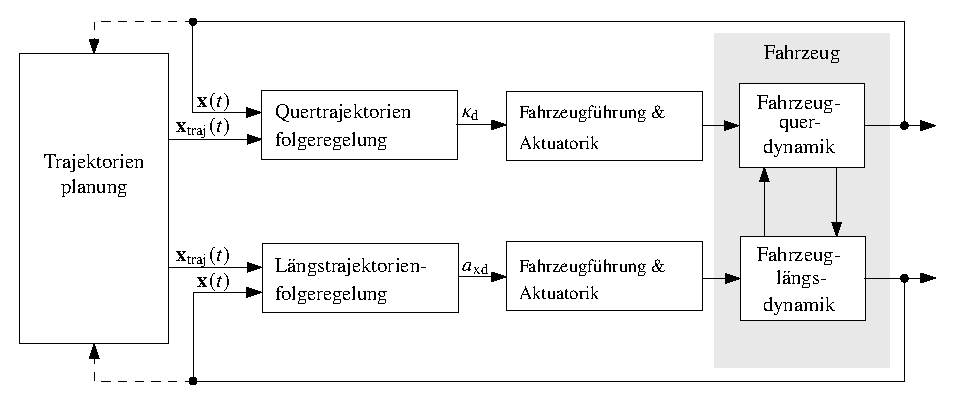
\includegraphics[width=12cm]{Bilder/04/2dof_bf.eps}
%	\caption{Anwendung der Zwei-Freiheitsgrade-Regelungsstruktur auf die Bahnführungsebene}
%	\label{abb_2dof_bf}
%\end{figure}

%Abb.  \ref{abb_2dof_bf} veranschaulicht die Anwendung der Struktur auf die Bahnführungsebene.  
Da die Trajektorienplanung durch Berücksichtigung des fahrdynamischen Potenzials die fahrdynamischen Grenzen und die Beschränkungen der verwendeten Aktuatorik berücksichtigt, kann die nachgelagerte Regelung in einen Quer- und Längsanteil aufgeteilt werden.
\subsection{Trajektorienfolgeregelung}
Ziel der Trajektorienfolgeregelung ist die Umsetzung der geplanten Trajektorie $\mathbf{x}_\mathrm{traj}(t)$ mit den Stellgrößen der Bahnführungsebene $\kappa_\mathrm{d}$ und $\aXD$.  Dabei wird auf die Zwei-Freiheitsgradestruktur gesetzt.  Diese wird zunächst kurz vorgestellt und anschließend auf die Quer- und Längsregelung angewandt.  
Die Zwei-Freiheitsgradestruktur ist eine häufig eingesetzte Methode zur Lösung von Trajektorienfolgeproblemen.  Abb. \ref{fig:2DOF} veranschaulicht die übliche Umsetzung.

\begin{figure}[htp!]
\centering
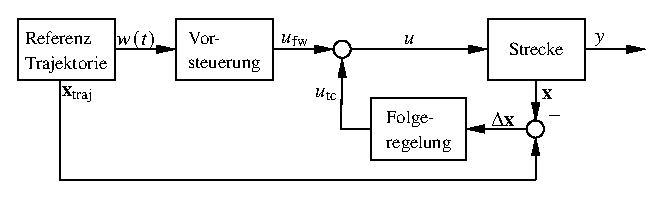
\includegraphics{Bilder/04/2DOF.eps}
\caption{Zwei-Freiheitsgrade-Regelungsstruktur}
\label{fig:2DOF}
\end{figure}

Es stehen sowohl der Zustandsverlauf der Trajektorie $\mathbf{x}_\mathrm{traj}$ als auch der gemessene Zustand $\mathbf{x}$ zur Verfügung.  Die unterlagerte Strecke wird durch die Dynamik $\tilde G$ und die Totzeit $T_\mathrm{D}$ beschrieben.  Entsprechend der Zwei-Freiheitsgrade-Regelung ergibt sich die Stellgröße $u$ mit 
\begin{equation}
u=u_\mathrm{fw}+u_\mathrm{tc}
\end{equation}
aus dem dominanten Vorsteuerungsanteil $u_\mathrm{fw}$ und dem Regelungsanteil $u_\mathrm{tc}$.  Ersterer hat die Aufgabe die unterlagerte Streckendynamik zu berücksichtigen und das Regelungsziel $w(t)$ bei Abwesenheit von Störungen zu realisieren:
\begin{equation}
u_\mathrm{fw} =  \tilde G^{-1} w(t+T_\mathrm{D})
\label{eq_u_ffw}
\end{equation}
Da die Trajektorie als Zustandsverlauf über der Zeit dargestellt ist, können bekannte Totzeiten direkt kompensiert werden indem die Trajektorie zur Berechnung der Führungsgröße zum um die Totzeit $T_\mathrm{D}$ prädizierten Zeitpunkt $t+T_\mathrm{D}$ ausgewertet wird.  

Da das Regelungsziel bereits zum Großteil durch die Vorsteuerung erreicht wird,  kann die Folgeregelung vergleichsweise einfach umgesetzt werden und auch eine Linearisierung des Systems entlang der Referenztrajektorie ist zulässig.  So wird die Stellgröße $u_\mathrm{tc}$ häufig durch Rückführung der Regelfehler $\Delta \mathbf{x} =  \mathbf{x}_\mathrm{traj}- \mathbf{x}$ mittels der Verstärkungsfaktoren $\mathbf{k}$:
\begin{equation}
u_\mathrm{tc} = \mathbf{k} \Delta \mathbf{x}
\end{equation}
berechnet.

Abb.  \ref{abb_zustaende_tfc} veranschaulicht die Zustände der geplanten Trajektorie sowie die gemessen Fahrzeugzustände.  
%
\begin{figure}[ht]
	\centering
	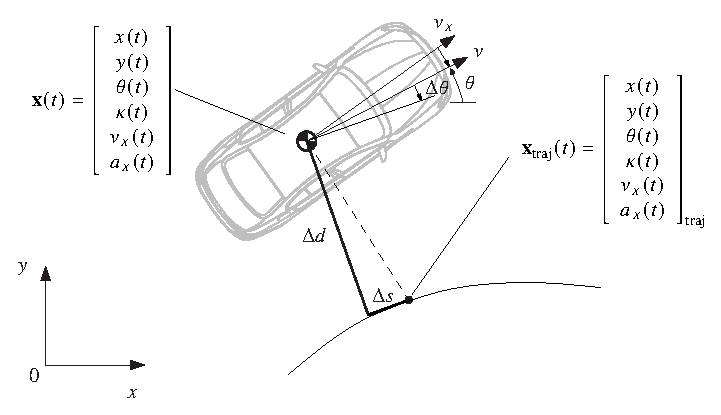
\includegraphics[width=0.9\textwidth]{Bilder/04/koordinaten_bahnfuehrung.eps}
	\caption{Darstellung der Zustandsgrößen der Trajektorenfolgeregelung}
	\label{abb_zustaende_tfc}
\end{figure}
%
In Querrichtung werden die Regelabweichungen zur geplanten Trajektorie über die Querablage $\Delta d$ und die Winkelabweichung $\Delta \theta$ und in Längsrichtung über den Längspositionsfehler $\Delta s$ und den Geschwindigkeitsregelfehler $\Delta v$ beschrieben:
\begin{equation}
\left[
\begin{matrix}
\Delta s \\ 
\Delta d \\ 
\Delta \theta \\ 
\Delta v_x
\end{matrix} 
\right]
:=
\left[
\begin{matrix}
\left[
\begin{matrix}
\cos \theta_\mathrm{traj} & \sin \theta_\mathrm{traj} \\ 
-\sin \theta_\mathrm{traj} & \cos \theta_\mathrm{traj} 
\end{matrix} 
\right]
\left[
\begin{matrix}
x_\mathrm{traj} -x\\ 
y_\mathrm{traj} -y
\end{matrix} 
\right]\\
\theta_\mathrm{traj} - \theta \\ 
\vXT- v_x.
\end{matrix} 
\right]
\label{eq_tfc_regelfehler}
\end{equation}
%
%
Der Kurswinkel $\theta$ ergibt sich dabei aus der Summe des Gierwinkels $\psi$ und Schwimmwinkels $\beta$.  Die Fehlerdynamik berechnet sich mit $v=\frac{v_x}{\cos{\beta}}$ zu
\begin{subequations}
\begin{align}
 \Delta \dot s &=  \vXT\kappa_\mathrm{traj} \Delta d + \vXT- v  \cos \Delta \theta \\
 \Delta \dot d &=   - \vXT\kappa_\mathrm{traj} \Delta s +  v \sin \Delta \theta \\
 \Delta \dot v_x &= \aXT- a_x \\
 \Delta \dot \theta &=  v _\mathrm{x,traj} \kappa_\mathrm{traj} - v \kappa\label{eq_dgl_theta}
\end{align}
\end{subequations}
%
Vernachlässigt man die Querfehler in der Bildung der Längsfehler und umgekehrt und betrachtet kleine Abweichungen, so erhält man die vereinfachten, linearen Gleichungen
\begin{subequations}
\begin{align}
 \Delta \dot s &=   \Delta v_x \\
 \Delta \dot d &=    v_x  \Delta \theta.
 \label{eq_dgl_d}
\end{align}
\end{subequations}
Diese stellen häufig die Grundlage für den Entwurf von linearen Spurführungsreglern dar (siehe z.B.  \cite{Ackermann1995}).
%
%
\subsubsection{Quertrajektorienfolgeregelung}
Entsprechend des in Kapitel \ref{ch_3EM} vorgestellten Drei-Ebenen-Modells ist als Stellgröße der Querregelung die Sollkrümmung $\kappa_\mathrm{d}$ definiert.  Die Dynamik der unterlagerten Regelung wird mit $\tilde G_{\kappa_\mathrm{d} \rightarrow \kappa }$ und der Totzeit $T_{\mathrm{D},\kappa}$ angenommen.  Entsprechend Gl.~(\ref{eq_u_ffw}) ergibt sich die Vorsteuerung der Quertrajektorienfolgeregelung zu
\begin{equation}
 \kappa_\mathrm{fw} = \tilde G_{\kappa_\mathrm{d} \rightarrow \kappa}^{-1}  \kappa_\mathrm{traj} (t+T_{\mathrm{D},\kappa}).
\end{equation}
Die Invertierung der Übertagungsfunktion kann mit den gängigen Methoden durchgeführt werden\footnote{Erfüllt die berechnete Trajektorie ausreichend Stetigkeitsanforderungen und kann so neben der Führungsgröße $\kappa_\mathrm{traj}(t)$ auch dessen Ableitungen bereitstellen, ist für die Invertierung der Streckendynamik kein Filter notwendig.}.\\
Die relevanten Regelfehler $\Delta d$ und $\Delta \theta$ lassen sich mit Gl.~(\ref{eq_tfc_regelfehler}) aus den gemessen und geplanten Zuständen berechnen.
Damit stehen alle notwendigen Informationen zur Verfügung und die Stellgröße der Querregelung berechnet sich zu
\begin{equation}
\kappa_\mathrm{d} = \kappa_\mathrm{fw} + \kappa_\mathrm{tc} = \tilde G_{\kappa_\mathrm{d} \rightarrow \kappa}^{-1}  \kappa_\mathrm{traj} (t+T_{\mathrm{D},\kappa})+ k_{\theta} \Delta \theta + k_d \Delta d
\end{equation}
mit den Verstärkungsfaktoren $k_{\theta}$ und $k_d$.  Die Verstärkungsfaktoren werden unter Zuhilfenahme der Bewegungsgleichen (\ref{eq_dgl_theta}) und (\ref{eq_dgl_d}) hergeleitet: Das Ziel von $\kappa_\mathrm{tc}$ ist es, Querabweichungen von der Zieltrajektorie asymptotisch zu unterdrücken: $\mathop {\lim }\limits_{t \to \infty } \Delta d(t) =0$.
Das Regelgesetz dazu resultiert unter Vernachlässigung der unterlagerten Dynamik direkt aus der Ableitung der Differenzialgleichung (\ref{eq_dgl_d}).  Durch dessen Ableitung erhält man
\begin{equation}
\Delta \ddot d = \dot v_x \Delta \theta + v_x \Delta\dot{{ \theta}} = a_x \Delta \theta - v_x^2 \kappa_\mathrm{tc}.
\end{equation}
%It has to satisfy a a second order homogeneous differential equation:
Fordert man als Wunschverhalten ein $PT_2$-Einschwingverhalten mit einer Wunschzeitkonstante $T_{\mathrm{tc},\kappa}$
%
\begin{equation}  
T_{\mathrm{tc},\kappa}^2 \Delta \ddot d + 2T_{\mathrm{tc},\kappa} \Delta \dot d + \Delta d = 0
\end{equation}
und löst nach dem Stellsignal $\kappa_\mathrm{tc}$ auf,  resultiert
\begin{equation}
\kappa_\mathrm{tc} = \Delta  \theta\, \underbrace{\frac{a_x T_{\mathrm{tc},\kappa}^2 + 2 v_x  T_{\mathrm{tc},\kappa}}{T_{\mathrm{tc},\kappa}^2 v_x^2}}_{k_\theta} + \Delta d \, \underbrace{\frac{1}{T_{\mathrm{tc},\kappa}^2 v_x^2}}_{k_d}.
\end{equation}
Dieses Regelgesetz garantiert das asymptotische Abklingen von Querablagefehlern\footnote{Um stationäre Genauigkeit zu erreichen,  muss der Kurswinkel korrekt erfasst werden.  Da der darin enthaltene Schwimmwinkel meist nur über einen Beobachter ermittelt wird,  kann bei nicht ausreichender Qualität ein zusätzlicher Beobachter auf Bahnführungsebene notwendig sein, vgl. \cite{Rathgeber2016}}.  Die Verstärkungsfaktoren sind geschwindigkeitsabhängig und stellen damit ein analytisches,  geschwindigkeitsabhängiges \textit{Gain Scheduling} dar. Unabhängig von der Fahrzeuggeschwindigkeit stellt sich das gleiche dynamische Verhalten des geregelten Systems ein.
\subsubsection{Längstrajektorienfolgeregelung}
Als Stellgröße der Längstrajektorienfolgeregelung ist die Sollbeschleunigung $\aXD$ definiert.  Die Dynamik der unterlagerten Regelung wird mit $\tilde G_{\aXD\rightarrow a_x }$ und der Totzeit $T_{\mathrm{D},a_x}$ angenommen. Die Längregelfehler $\Delta s$ und $\Delta v$ lassen sich entsprechend Gl.~(\ref{eq_tfc_regelfehler}) berechnen.  Damit ergibt sich das Regelgesetz
\begin{equation}
\aXD= a_{x,\mathrm{fw}} + a_{x,\mathrm{tc}} = \tilde G_{\aXD\rightarrow a_x}^{-1}  \aXT(t+T_{\mathrm{D},a_x})+ k_{v} \Delta v + k_s \Delta s
\end{equation}
mit den Verstärkungsfaktoren $k_v$ und $k_s$.  Diese werden analog zur Querregelung durch Forderung eines ideal gedämpften $PT_2$-Störunterdrückungs-Verhaltens mit der Zeitkonstante $T_{\mathrm{tc},a_x}$ berechnet und man erhält das Stellgesetz
\begin{equation}
a_{x,\mathrm{tc}} = \Delta v \underbrace{\frac{2}{T_{\mathrm{tc},a_x}}}_{k_v} + \Delta s \underbrace{\frac{1}{T_{\mathrm{tc},a_x}^2}}_{k_s}.
\end{equation}


\FloatBarrier

%\section{Fahrzeugführungsebene längs/quer}
\label{ch_Fahrzeugführungsebene}

Im vorangegangenen Abschnitt wurde dargestellt, wie die Trajektorienfolgeregler durch Vorgabe einer Sollkrümmung $\kappa_\mathrm{d}$ und einer Solllängsbeschleunigung $a_{x\mathrm{d}}$ das Fahrzeug auf der geplanten Trajektorie führen. Dieser Abschnitt befasst sich nun mit den Regelungsstrukturen der Fahrzeugführungsebene, die diese Vorgaben durch Ansteuerung der Aktuatoren umsetzten. Dabei müssen eine Reihe von Anforderungen berücksichtigt werden, die sich aus der im Abschnitt \ref{S:Intro} vorgestellten Regelungsaufgabe ergeben. Insbesondere ist die Fahrzeugsführungsebene für Störunterdrückung und Robustheit bezüglich der Fahrzeug- und Aktuatoreigenschaften verantwortlich. Außerdem findet auf dieser Ebene die direkte Interaktion mit dem Fahrer statt, bei der die verschiedenen Kooperationsgrade berücksichtigt werden müssen.

\subsection{Störgrößenbeobachter (Disturbance Observer) - Grundstruktur}\label{subS:DO_Basic}

Die Bewegung des Fahrzeugs unterliegt sowohl in Längs- als auch in Querrichtung nicht vernachlässigbaren Störungen\index{Störung}. Diese müssen durch geeignete Reglerstrukturen in Abhängigkeit des gewünschten Autonomiegrades mehr oder weniger vollständig kompensiert werden.
Ein klassischer I-Anteil wäre dazu prinzipiell in der Lage, bietet aber nicht die notwendigen Freiheitsgrade, sein Störunterdrückungsverhalten an den gewünschten Autonomiegrad anzupassen.

%In die erste Klasse fällt beispielsweise ein klassischer I-Anteil. Dieser ist in der Lage, bestimmte Störungen stationär zu unterdrücken.
%Dabei kann jedoch nur das Zeitverhalten des Ausregelns der Störung nicht aber der zu unterdrückende Anteil der Störung eingestellt werden.
%Für die Anwendung in einer Architektur mit variablem Autonomiegrad liegt in dieser Unnachgiebigkeit ein wesentlicher Grund, weswegen ein klassischer I-Anteil nicht geeignet ist
 
Zum Einsatz kommen daher Störgrößenbeobachter (engl. \emph{disturbance observer}, DO, siehe \cite{Ohnishi1987}) mit gleichzeitiger Kompensation, deren grundlegende Struktur in \refFig{DO_Basic} dargestellt ist. Die Struktur ist augenfällig verwandt mit IMC (engl. \emph{internal model control}, siehe \cite{GarciaMorari82}), welches in \refFig{IMC_Basic} dargestellt ist. Beide Strukturen weisen bei richtiger Wahl der Übertragungsfunktion $Q(s)$ sehr gute Störunterdrückung auf. DO bietet darüber hinaus im Kontext der angestrebten Einstellbarkeit der Störunterdrückung intuitiv nachvollziehbare Eingriffsmöglichkeiten. Außerdem ist das Führungsverhalten bei DO unter der Annahme $G\approx\tilde G$ unabhängig von $Q$ und kann über einen überlagerten Regler getrennt eingestellt werden.


%Lösungen aus der zweiten Klasse haben im Kontext variabler Autonomiegrade den Vorteil, dass die Unterdrückung der Störungen nicht nur hinsichtlich des Zeitverhaltens, sondern auch hinsichtlich des stationären Verhaltens gezielt beeinflusst werden kann. Außerdem ist es damit möglich, Führungs- und Störverhalten der Regelung unabhängig voneinander einzustellen.

%\refFig{DO_allg} zeigt eine mögliche Struktur für einen Störgrößenbeobachter mit gleichzeitiger Kompensation (Störunterdrückung). Diese Struktur hat bereits in vielen regelungstechnischen Anwendungen ihre positiven Eigenschaften unter Beweis gestellt, siehe Literatur.


\begin{figure}[htp!]

\begin{minipage}[t]{0.5\textwidth}
\centering
\import{Bilder/DO_allg/}{DO_Basic_compact.pdf_tex}
\parbox{0.9\textwidth}{\captionof{figure}{Grundstruktur des Störgrößenbeobachters (\emph{disturbance observer}, DO) mit Kompensation}\label{fig:DO_Basic}}
\end{minipage}
\begin{minipage}[t]{0.5\textwidth}
\centering
\import{Bilder/DO_allg/}{IMC_Basic_compact.pdf_tex}
\parbox{0.8\textwidth}{\captionof{figure}{Grundstruktur \emph{internal model control} (IMC)}\label{fig:IMC_Basic}}
\end{minipage}

\end{figure}



In \refFig{DO_Basic} steht $G$ für das dynamische Verhalten einer Reglestrecke, $\tilde G$ ist eine Näherung dieses Verhaltens. Durch die Invertierung von $\tilde G$ im Rückführpfad wird der Ausgang $y$ in eine virtuelle Eingangsgröße $\tilde u$ umgerechnet, die anschließen mit dem tatsächlichen Eingang $u$ verglichen wird. Da die Invertierung von $\tilde G$ üblicherweise nicht realisierbar ist, wird das Tiefpassfilter $Q$ eingeführt, sodass $Q\tilde G$ realisierbar wird. Die damit einhergehende Verzögerung von $\tilde u$ im Vergleich zu $u$ wird beim Vergleich berücksichtigt, indem auch $u$ das Tiefpassfilter $Q$ durchläuft. Die Differenz $Qu-\tilde u$ liefert auf Grundlage dieser Interpretation eine Abschätzung $\tilde d_1$ der Eingangsstörung $d_1$, wobei die Auswirkung von $d_2$ auf den Eingang zurückgerechnet auch berücksichtigt wird. Durch die Rückführung von $-\tilde d_1$ auf den Eingang werden die Störungen $d_1$ und $d_2$ kompensiert.



%Darin ist $G$ die Übertragungsfunktion einer Regelstrecke, für die die Näherung $\tilde G$ existiert. Auf die Strecke wirken verschiedene Störungen, die hier als Eingangsstörung $d_1$ und Ausgangsstörung $d_2$ modelliert sind. Unter der Annahme, dass $\tilde G\approx G$ und zunächst mit der Näherung $Q\approx 1$ kann der Block $Q \tilde G ^{-1}$ wie folgt interpretiert werden: der durch die Störungen $d_1$ und $d_2$ beeinflusste Ausgang $y$ der Strecke wird auf eine virtuelle Eingangsgröße $\tilde u$ so zurückgerechnet, dass $y$ dann der ungestörte Ausgang von $G$ bei Anregung mit $\tilde u$ wäre, wobei $\tilde u$ den Einfluß der Störungen enthält. Subtrahiert man nun $u$ von $\tilde u$ bleibt eine Abschätzung $\tilde d$ für die Wirkung aller Störungen $d_1$ und $d_2$ bezogen auf den Eingang übrig. Wird $\tilde d$ dann wiederum von $u_\mathrm r$ subtrahiert, so werden damit die Störungen $d_1$ und $d_2$ kompensiert.
%
%Da $\tilde G$ im Normalfall nicht invertierbar, $\tilde G^{-1}$ also nicht realisierbar ist, wird das Filter $Q$ eingeführt. Damit $Q \tilde G ^{-1}$ realisierbar wird, muss $Q$ den Nullstellenüberschuss von $\tilde G ^{-1}$ ausgleichen, also Tiefpassverhalten haben. Die damit einhergehende Verzögerung von $\tilde u$ muss auch auf $u$ angewendet werden, bevor die Differenz $\tilde u-Qu$ gebildet wird.

Die Übertragungsfunktionen der Störungen $d_1$ und $d_2$ auf den Ausgang $y$ ergeben sich dann zu 
\begin{equation}
\setlength\arraycolsep{11pt}
\begin{matrix}
G_{d_1\rightarrow y} = \frac{G\tilde G(1-Q)}{\tilde G(1-Q)+GQ}\Biggr\rvert_{Q=1}=0
&
G_{d_2\rightarrow y} = \frac{\tilde G(1-Q)}{\tilde G(1-Q)+GQ}\Biggr\rvert_{Q=1}=0
\end{matrix}
\label{eq:DO1}
\end{equation}

Beide Störübertragungsfunktionen in \refEq{DO1} werden stationär $0$, wenn die stationäre Verstärkung von $Q$ zu 1 gewählt wird. Das dynamische Verhalten der Störunterdrückung ist unter Berücksichtung des Messrauschens $n$ über die Wahl der Pole von $Q$ einstellbar.


Die Verwandschaft des hier eingesetzten Störgrößenbeobachters mit einem klassischen I-Anteil wird offensichtlich, wenn man die linke Rückkopplungschleife im Signalfluss von \refFig{DO_Basic} wie in \refFig{DO_Int} dargestellt umformt.

\begin{figure}[htp!]
\centering
\import{Bilder/DO_allg/}{DO_Int.pdf_tex}
\caption{Rückkopplung des Eingangs $u$ im Störgrößenbeobachter ergibt in der Grundform PI-Verhalten}
\label{fig:DO_Int}
\end{figure}

Ist $Q(s)$ ein Tiefpassfilter der Form
\begin{equation}
Q(s)=\frac{1}{1 + \lambda_1 s + \lambda_2 s^2 + \hdots}
\end{equation}
dann ist die Übertragungsfunktion von $(u_\mathrm r{-}\tilde u)$ zu $u$
\begin{equation}
G_\mathrm{PI}(s)=1+\frac{1}{s(\lambda_1+\lambda_2 s + \hdots)}
\end{equation}
also eine Kombination aus P-Verhalten mit Verstärkung 1 und in Abhängigkeit der Koeffizienten
$\lambda_i$ mehr oder weniger verzögertem I-Verhalten. Folglich verhält sich $u$ im oberen Frequenzbereich wie $u_\mathrm{r}$, im unteren Frequenzbereich wird sich hingegen $u$ so einstellen, dass $u_\mathrm{r}-\tilde u=0$.

Neben der störunterdrückenden Wirkung des Stögrößenbeobachters ist eine weitere Eigenschaft dieser Struktur von großem Vorteil, die zumindest qualitativ offenbar wird, wenn man das Übertragungsverhalten von $u_\mathrm{r}$ nach $y$ für $Q=1$ betrachtet.
\begin{equation}
G_{u_\mathrm{r}\rightarrow y}=\frac{G\tilde G}{\tilde G(1-Q)+GQ}
\Biggr\rvert_{Q=1}=\tilde G\label{eq:DO3}
\end{equation}
\refEq{DO3} bedeutet, dass der Störgrößenbeobachter das Verhalten von $\tilde G$ annimmt. Dies hat zwei Konsequenzen: zum einen ist der Störgrößenbeobachter robust auch bei größeren Abweichungen zwischen dem realen Streckenverhalten und $\tilde G$, zum anderen kann diese Eigenschaft als Entwurfsfreiheitsgrad genutzt werden, um mit $\tilde G$ das Verhalten des störgrößenkompensierten Systems vorzugeben.

Definiert man in Anlehnung an mechanische Systeme die Steifigkeit einer Regelung als Verhältnis der Größe einer Störung (Kraft) zu der durch die Störung verursachten Abweichung vom Nominalverhalten (Verformung), so ergibt sich bei der hier vorliegenden stationär vollständigen Störunterdrückung eine unendlich hohe Steifigkeit bzw. eine Nachgiebigkeit von 0.


%Rechnerisch würde sich mit der Grundstruktur des Störgrößenschätzers aufgrund der genannten Eigenschaften eine stationär unendlich hohe Steifigkeit bezüglich der auftretenden Störungen ergeben.

In den beiden folgenden Abschnitten soll nun gezeigt werden, wie diese hohe Steifigkeit zum einen gezielt reduziert bzw. die Nachgiebigkeit erhöht werden kann und wie es zum anderen gelingt, bestimmte Störungen im Sinne einer Selektivität überhaupt nicht auszuregeln.




%%%%%%%%%%%%%%%%%%%%%%%%%%%%%%%%%%%%%%%%%%%%%%%%%%%%%%%%%%%%%%%%%%%%%%%%%%%%%%%%%%%%%%%%%%

\subsection{Einstellbare stationäre Genauigkeit}\label{subS:DO_Scale_Lim}
Da im Störgrößenbeobachter explizit die beobachtete Störung zunächst ermittelt und dann durch Aufschaltung kompensiert wird, ist es sehr leicht möglich, das Maß der Kompensation einstellbar zu gestalten. Im wesentlichen wird dazu die Struktur aus \refFig{DO_Basic} wie in \refFig{DO_Scale_Lim} dargestellt durch die Möglichkeit einer Skalierung und Begrenzung der aufgeschalteten Störung ergänzt. 

\begin{figure}[htp!]
\centering
\import{Bilder/DO_allg/}{DO_Scale_Lim.pdf_tex}
\caption{Störgrößenbeobachter mit Skalierung und Begrenzung der aufgeschalteten Störung}
\label{fig:DO_Scale_Lim}
\end{figure}

Mit der Skalierung $k$ ändern sich die Störübertragungsfunktionen \refEq{DO1} zu
\begin{equation}
\setlength\arraycolsep{11pt}
\begin{matrix}
G_{d_1\rightarrow y} = \frac{G\tilde G(1-kQ)}{\tilde G(1-kQ)+kGQ} & 
G_{d_2\rightarrow y} = \frac{\tilde G(1-kQ)}{\tilde G(1-kQ)+kGQ}
\end{matrix}\label{eq:DO5}
\end{equation}
Die Auswirkung von $k$ kann unter den Annahmen $Q=1$ und $G\approx\tilde G$ plausibel abgeschätzt werden. \refEq{DO5} vereinfacht sich dann zu
\begin{equation}
\setlength\arraycolsep{11pt}
\begin{matrix}
G_{d_1\rightarrow y}\big\rvert_{Q=1, \tilde G \approx G} = G(1-k) & 
G_{d_2\rightarrow y}\big\rvert_{Q=1, \tilde G \approx G} = (1-k)
\end{matrix}\label{eq:DO7}
\end{equation}

Das bedeutet, dass von der ursprünglichen Auswirkung der Störungen auf den Ausgang $y$ ($Gd_1$ im Falle von $d_1$ und $d_2$ im Falle von $d_2$) ein Anteil $(1-k)$ bleibt bzw. dass nur ein Anteil $k$ der Störungen kompensiert wird, wenn der Störgrößenbeobachter mit einer solchen Skalierung eingesetzt wird.

Mit Ähnlichen Abschätzungen kann die Auswirkung einer Begrenzung im Kompensationspfad greifbar gemacht werden. Darüber hinaus ist die Begrenzung eine wirksame Anti-Windup-Maßnahme, die notwendig ist, wenn die Srecke $G$ im realen System Stellgrößenbegrenzungen enthält.

Im Abschnitt \ref{subS:DO_Delta} wird im Detail vorgestellt, wie Skalierung und Begrenzung eingesetzt werden, um den Störgrößenbeobachter in der Lenkwinkelregelung gezielt nachgiebig  machen.

\subsection{Selektive Kompensation von Störungen}
In diesem Abschnitt wird eine weiter Adaption der Grundstruktur des Störgrößenbeobachters aus Abschnitt \ref{subS:DO_Basic} vorgestellt, die den Störgrößenbeobachter ausgewählten Störungen gegenüber blind macht, d.h., das Übertragungsverhalten dieser Störungen auf den Ausgang unbeeinflusst lässt.
%
Dies gelingt unter der Voraussetzung, dass eine zusätzliche Meßgröße $y_1$ innerhalb der Regelstrecke, z.B. am Ausgang des Aktuators, abgegriffen werden kann, welche nur die Störungen enthält, die zu ignorieren sind. Der Streckenausgang $y$ enthält alle Störungen, siehe \refFig{DO_Modified}.
Der Vergleich von $y_1$ und dem durch die Inverse der Teilstrecke $G_2$ zurückgerechnete Ausgang liefert nun ein Maß $\tilde d_{12}$ nur für die Störungen $d_{12}$ und $d_{22}$ an der Teilstrecke $G_2$. Durch Multiplikation mit $G_1^{-1}$ wird daraus ein auf den Eingang der Strecke umgerechneter Wert $\tilde d$, der bei Aufschaltung die Wirkung der Störungen
$d_{12}$ und $d_{22}$ kompensiert, die Störungen $d_{11}$ und $d_{21}$ jedoch ignoriert.
Wie im Falle der Grundstruktur des Störgrößenbeobachters werden Tiefpaßfilter $Q_1$ und $Q_2$ mit stationärer Verstärkung $1$ benötigt, um das Invertieren der Strecke realisierbar zu machen und um das dynamische Verhalten des Beobachters auszulegen.

\begin{figure}[htp!]
\centering
\import{Bilder/DO_allg/}{DO_Selective.pdf_tex}
%\import{Bilder/DO_allg/}{DO_Modified.pdf_tex}
\caption{Grundstruktur eines selektiven Störgrößenbeobachters zur Kompensation der Störungen $d_{12}$ und $d_{22}$.}
\label{fig:DO_Modified}
\end{figure}

Die Störübertragungsfunktionen sind dann für $Q_1=1$ und $Q_2=1$ (stationär und unterer Frequenzbereich)
\begin{equation}
\begin{matrix*}[l]
G_{d11}&=&G_1 G_2 \tilde G_1 \tilde G_2 \cdot D^{-1} & \hspace{6pt} &
G_{d12}&=&G_2 \tilde G_2 (\tilde G_1 - G_1) \cdot D^{-1} \\
G_{d21}&=&G_2 \tilde G_1 \tilde G_2 \cdot D^{-1}& \hspace{6pt} &
G_{d22}&=&\tilde G_2 (\tilde G_1 - G_1) \cdot D^{-1}
\end{matrix*}
\label{eq:DoSel01}
\end{equation}

mit dem gemeinsamen Nenner $D=\tilde G_2(\tilde G_1 - G_1)+G_1 G_2$.
Es ist leicht zu erkennen, dass die Bedingung $\tilde G_1=G_1$ in den relevanten Frequenzbereichen erfüllt sein muss, damit die Störungen $d_{12}$ und $d_{22}$ dort vollständig kompensiert werden. Mit dieser Bedingung vereinfacht sich \refEq{DoSel01} zu
\begin{equation}
\begin{matrix*}[l]
G_{d11}\bigr\rvert_{\tilde G_1 = G_1}&=&G_1 \tilde G_2 & \hspace{12pt} &
G_{d12}\bigr\rvert_{\tilde G_1 = G_1}&=&0\\
G_{d21}\bigr\rvert_{\tilde G_1 = G_1}&=&\tilde G_2 & \hspace{12pt} &
G_{d22}\bigr\rvert_{\tilde G_1 = G_1}&=&0
\end{matrix*}
\label{eq:DoSel02}
\end{equation}

$d_{11}$ und $d_{21}$ behalten also im wesentlichen das selbe Übertragungsverhalten auf den Ausgang $y$ wie ohne den Störgrößenbeobachter. $d_{12}$ und $d_{22}$ werden ausgeregelt.
 
Die Übertragungsfunktion $G_{u_\mathrm{r}\rightarrow y}$ ist gleich $G_{d11}$ und damit ebenfalls $G_1\tilde G_2$. Es kann also auch bei dieser Form des Störgrößenbeobachters ein Teil des Streckenverhaltens durch die Wahl von $\tilde G_2$ vorgegeben werden bzw. ist dieser Störgrößenbeobachter ebenfalls robust gegenüber Abweichungen zwischen $\tilde G_2$ und $G_2$.
$\tilde G_1$ muss hingegen mit $G_1$ sehr gut übereinstimmen.



%%%%%%%%%%%%%%%%%%%%%%%%%%%%%%%%%%%%%%%%%%%%%%%%%%%%%%%%%%%%%%%%%%%%%%%%%%%%%%%%%%%%%%%%%%%

\subsection{Störgrößenbeobachter Krümmung}\label{subS:DO_Kappa}
Ziel des Krümmungs-Störgrößenbeobachters $\mathrm{DO}_\kappa$ ist es, die gegebene Sollkrümmung der Bahnführungsebene $\kappa_\mathrm{d}$ stationär genau umzusetzen.  Dabei sollen sämtliche Seitenkraftstörungen, die auf das Fahrzeug wirken unterdrückt werden.  Diese können von Seitenwinden,  hängenden Fahrbahnen etc. verursacht werden.  Die Herausforderung dabei ist es, bei kooperativen Kundenfunktionen die Fahrereingriffe nicht als Störung zu unterdrücken um ein nachgiebiges Reglerverhalten darstellen zu können.  Wie im vorangegangen Abschnitt bereits dargestellt, kann die Struktur des selektiven Störgrößenbeobachters unter Rückführung einer Hilfsgröße diesen Zielkonflikt auflösen.  

Zur Beeinflussung der Querdynamik wird im Folgenden nur von Beeinflussung der Vorderachslenkung ausgegangen, sodass die Control Allocation $\mathrm{CA}_\kappa$ entfällt.  Mittels der angenommenen stationären Verstärkung $\tilde k_\kappa$ kann die Sollkrümmung zur Ansteuerung der Lenkwinkelregelung in einen Solllenkwinkel $\delta_\mathrm{d}$ umgerechnet werden:
\begin{equation}
\delta_\mathrm{d} = \tilde k_\kappa^{-1} \kappa_{\delta\mathrm{d}}
\end{equation}
Als Modell für den Entwurf des Störgrößenbeobachters dienen die Gleichungen (\ref{eq:GL2}) und (\ref{eq:Gkappa}).  Dementsprechend ergibt sich die Krümmung als Folge des Übertragungsverhaltens der geregelten Lenkung $G_\delta$ und des Einspurmodells $G_\kappa$.  
%Als Hilfsgröße wird dazu der gemessene Lenkwinkel $\delta$ mittels der Ackermann-Verstärkung umgerechnet: 
%\begin{equation}
%\kappa_\delta = K_{Ackermann} \delta
%\end{equation}
%$\kappa_\delta$ gibt somit die Krümmung wieder die das Fahrzeug bei Abwesenheit von Störungen stationär einnimmt.  Diese wird im Störgrößenbeobachter mit der gemessen Ist-Krümmung verglichen.
Als Hilfsgröße wird der gemessene Lenkwinkel $\delta$ zurückgeführt.  Dieser gibt sowohl das gestellte Moment der unterlagerten Lenkwinkelregelung als auch das Fahrerlenkmoment $\tau_{\delta,\mathrm{drv}}$ wider.  Die auf das Fahrzeug wirkenden und zu unterdrückenden Seitenkraftstörungen $z_\kappa$ sind dagegen nur in der gemessenen Krümmung $\kappa$ sichtbar.  Abb.~\ref{fig:DO_kappa} zeigt die Umsetzung des Krümmungs-Störgrößenbeobachters im Blockschaltbild.  Dessen Ausgang ergibt sich zu:
\begin{equation}
\kappa_\mathrm{do} = \tilde k_\kappa Q_\delta \tilde G_\delta^{-1} \left( Q_\kappa \delta - Q_\kappa \tilde{G}_\kappa^{-1} \kappa \right)
\end{equation}
Die gesamte Stellgröße $\kappaDPrime$ berechnet sich als Summe von $\kappa_\mathrm{d}$ und $\kappa_\mathrm{do}$.  Zur Realisierung der Invertierungen der angenommenen Übertragungsfunktionen $\tilde G_\delta$ und $\tilde G_\kappa$ sind die Tiefpassfilter $Q_\delta$ und $Q_\kappa$ notwendig.  
%
\begin{figure}[ht]
	\centering
	\includegraphics{Bilder/DO_allg/DO_kappa.eps}
	\caption{Selektiver Störgrößenbeobachter auf Krümmungsebene zur Kompensation der Störung $z_\kappa$ ohne Kompensation des Fahrerhandmoments $\tau_{\delta,\mathrm{drv}}$}
	\label{fig:DO_kappa}
\end{figure}
%
Störungen $z_\kappa$ werden mit dieser Struktur stationär genau unterdrückt, wohingegen Fahrerinteraktionen nicht als Störungen interpretiert und ausgeregelt werden.  Auch Anti-Wind-Up Maßnahmen für etwaige Limitierung der Stellgrößen im Aktuator sind nicht notwendig da der  gemessene Lenkwinkel $\delta$ im Gegensatz zur Stellgröße $\delta_\mathrm{d}$ bereits die Limitierung enthält. Der über den Störgrößenbeobachter geschlossene Regelkreis prägt näherungsweise das nominelle Übertragungsverhalten 
\begin{equation}
\tilde G_{\kappa_\mathrm{d}\rightarrow \kappa} \approx \tilde k_\kappa^{-1} \tilde G_\delta \tilde G_\kappa
\end{equation}
auf.  Parameterschwankungen können so beherrscht und die Übertragungsfunktion für den Entwurf der Trajektorienfolgergelung innerhalb der Bahnführungsebene genutzt werden.
%
\subsection{Störgrößenbeobachter Längsbeschleunigung}
Analog zur Krümmungsregelung wird der Entwurf der Längsregelung durchgeführt: Mittels eines Störgrößenbeobachters wird die stationär genaue Umsetzung der Sollbeschleunigung $\aXD$ sichergestellt.  Auch hier wird durch Rückführung einer Hilfsgröße erreicht, dass Fahrerinteraktionen nicht als Störungen unterdrückt werden.  Dazu wird das sich einstellende Summenradmoment $\tau_{x}$ benutzt.  Dieses stellt sich in Folge der Fahrermomente über Gas- und Bremspedal und den Vorgaben durch die Funktion ein.  Als Modell für den Entwurf dient das angenommen Übertragungsverhalten entsprechend Gleichung (\ref{eq:GLong}) und (\ref{eq:Gwhl}).  Die geforderte Sollbeschleunigung wird über die angenommen Fahrzeugparameter $\tilde m$ und $\tilde r$ in ein Sollradmoment umgerechnet:
\begin{equation}
\tau_{x\mathrm{d}} = \aXD \tilde m \tilde r
\end{equation}
$\tilde m$ und $\tilde r$ stehen als Messgrößen im Fahrzeug zur Verfügung und werden durch Schätzverfahren ermittelt.  Die Verteilungslogik auf Antrieb und  Bremse ($\mathrm{CA}_x$) weißt durch im nächsten Abschnitt vorgestellte Logik näherungsweise das Übertragungsverhalten 1 auf und wird deswegen im Entwurf des Störgrößenbeobachters vernachlässigt.

Abb. \ref{fig:DO_acceleration} zeigt die Umsetzung des selektiven Störgrößenbeobachters zur Unterdrückung der Störungen $z_{a_x}$.  Die Stellgröße berechnet sich zu
\begin{equation}
a_\mathrm{x,do} = Q_{\tau_x} \left(\tilde m \tilde r\tilde G_{\tau_x}\right)^{-1} \left( Q_{a_x} \tau_{a_x} - Q_{a_x} \tilde{G}_{a_x}^{-1} a_x \right).
\end{equation}
Zur Realisierung der Invertierungen der angenommenen Übertragungsfunktionen $\tilde G_{\tau_x}$ und $\tilde G_{a_x}$ sind zwei Filter $Q_{\tau_x}$ und $Q_{a_x}$ notwendig.  Der so geschlossene Regelkreis verhält sich näherungsweise wie
\begin{equation}
\tilde G_{a_\mathrm{x,d}\rightarrow a_x} \approx \tilde m \tilde r\tilde G_{\tau_x}  \tilde G_{a_x}.
\end{equation}
% 
Störungen $z_{a_x}$ werden kompensiert,  wohingegen das Fahrerantriebsmoment $\tau_\mathrm{mot,drv}$ und Fahrerbremsmoment $\tau_\mathrm{brk,drv}$ nicht unterdrückt werden.
\begin{figure}[ht]
	\centering
	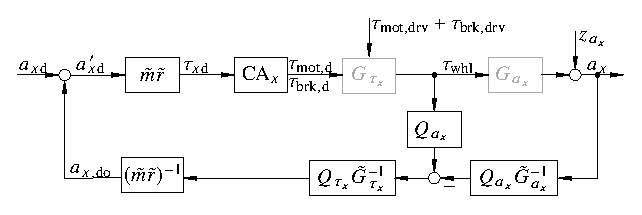
\includegraphics{Bilder/DO_allg/do_acceleration.eps}
	\caption{Selektiver Störgrößenbeobachter auf Beschleunigungsebene zur Kompensation der Störung $z_a$ ohne Kompensation des Fahrermoments $\tau_\mathrm{mot,drv}$ und $\tau_\mathrm{brk,drv}$}
	\label{fig:DO_acceleration}
\end{figure}


%%%%%%%%%%%%%%%%%%%%%%%%%%%%%%%%%%%%%%%%%%%%%%%%%%%%%%%%%%%%%%%%%%%%%%%%%%%%%%

\subsection{Kooperativer Lenkwinkelregler mit Störgrößenbeobachter}\label{subS:DO_Delta}

Der Lenkwinkelregler, C\sus{$\delta$} in \refFig{LongLatOverview}, hat in der Fahrzeugquerführung die Aufgabe, den angeforderten Solllenkwinkel $\delta_\mathrm{d}$ umzusetzen. Dabei soll er je nach Kundenfunktion mehr oder weniger steif sowohl auf Störungen durch den Fahrer $\tau_{\delta,\mathrm{drv}}$ als auch auf äußere und innere Kräfte, die am Lenksystem auftreten, reagieren.

Das Problem, einem geregelten System eine definierte Steifigkeit bzw. Nachgiebigkeit zu verleihen, ist aus der Robotik bekannt und wird dort durch verschiedene Ansätze zur Impedanzregelung gelöst. Dabei lassen sich vereinfacht vier Grundstrukturen identifizieren:
\begin{enumerate}
\item die gewünschte Impedanz des Systems wird beim Entwurf durch die Wahl der Verstärkungsfaktoren realisiert (kommt ohne Kraftsensorik aus)\label{ImpCtrl1}
\item steife Positionsregelung mit überlagertem Admittanzmodell der gewünschten Systemdynamik (Admittanzarchitektur)
\item steife Kraftregelung mit überlagertem Impedanzmodell der gewünschten Systemdynamik (Impedanzarchitektur)
\item kombinierte Positions-/Kraftregelung im Sinne einer Mehrgößen- oder Zustandsregelung
\end{enumerate}

Der hier vorgeschlagene Lenkwinkelregler bedient sich bei diesen Ideen, um der Forderung nach einstellbarer Steifigkeit und stationärer Genauigkeit gerecht zu werden. Dabei tritt das Lenksystem, welches über den Drehstab mit dem Fahrer interagiert, an die Stelle eines Roboters, der über einen Kraftsensor mit seiner Umgebung interagiert.

Im wesentlichen besteht der Lenkwinkelregler aus zwei kaskadierten P-Reglern, $k_{\delta\mathrm{P}}$ und $k_{\delta\mathrm{D}}$ mit Vorsteuerung, deren Strecke das durch einen Störgrößenbeobachter nach \ref{subS:DO_Scale_Lim} störgrößenkompensierte Lenksystem ist, siehe \refFig{Zff}.


\begin{figure}[htp!]
\centering
\import{Bilder/Zff/}{Zff.pdf_tex}
\caption{Kooperativer Lenkwinkelregler mit Störgrößenbeobachter; Steifigkeit und stationäre Genauigkeit sind über die Signale $\eta$ und $\zeta$ einstellbar}
\label{fig:Zff}
\end{figure}


Als Streckenmodell $\tilde G$ kommt im Störgrößenbeobachter das Lenkungsmodell~1 ($G_{\tau\delta}$) zum Einsatz, welches in Abschnitt~\ref{subS:SteeringModels} eingeführt wurde.

Die Reglerparameter, welche Einfluß auf Steifigkeit und stationäre Genauigkeit haben, können von außen durch die Signale $\eta$ (Steifigkeit) und $\zeta$ (stationäre Genauigkeit) verändert werden.
Dieser Eingriff in die Reglerparameter entspricht in seinen Grundzügen der Variante \ref{ImpCtrl1} der Impedanzregelung. Durch die gewählte Reglerstruktur ist es beim Regler aus \refFig{Zff} jedoch möglich, Steifigkeit und stationäre Genauigkeit in Grenzen \emph{unabhängig} voneinander einzustellen.

Die Ansätze zur Impedanzregelung mit Kraftrückführung erfordern i.A. sehr hohe Reglerbandbreiten, da das Übertragungsverhalten von den Stellmomenten zur gemessenen Reaktionskraft typischerweise hohe Bandbreiten aufweist. Je nach Partitionierung des Reglers können diese Reglerbandbreiten im Fahrzeug eventuell nicht realisiert werden. Dennoch ist eine Rückführung des Fahrerhandmomentes $\tau_{\delta\mathrm{,drv}}$, welches teilweise eine passive Reaktion darstellt, erforderlich, wenn sich der Regler steif bzgl. aller Störungen jedoch nachgiebig bzgl. des Fahrers verhalten soll. Die hier vorgeschlagene Lösung entkoppelt das Stellmoment $\tau_{\delta\mathrm{d}}$ und das Reaktionsmoment $\tau_{\delta\mathrm{,drv}}$ (Fahrerhandmoment) in den relevanten Frequenzbereichen indem abhängig von $\tau_{\delta\mathrm{,drv}}$ jedoch zeitlich verzögert die verschiedenen Regleranteile reduziert werden. Dabei sind die Eingriffsschwellen und das Ausmaß der Reduktion wiederum von der gewünschten Steifigkeit $\eta$ abhängig.


%\begin{figure}[htp!]
%\centering
%\import{Bilder/ImpedanceAdmittance/}{impedance_control.pdf_tex}
%\caption{Impedanzarchitektur}
%\label{fig:ImpArch}
%\end{figure}


%%%%%%%%%%%%%%%%%%%%%%%%%%%%%%%%%%%%%%%%%%%%%%%%%%%%%%%%%%%%%%%%%%%%%%%%%%%%%%%%%%
\subsection{Ansteuerung Antrieb und Bremse}
Die Strategie zur (funktionsunabhängigen) Verteilung des Sollradmoments $\tauXDPrime$ auf die beiden Aktuatoren Antrieb und Bremse wird im Folgenden zunächst für den Fall ohne Fahrerinteraktion erläutert: 

Für das Sollantriebsmoment $\tau_\mathrm{mot,d}$ wird direkt das berechnete Sollmoment $\tauXDPrime$ verwendet: 
\begin{equation}
\tau_\mathrm{mot,d}=  \tauXDPrime.
\end{equation}
Zur Ansteuerung der Bremse wird dagegen eine Fallunterscheidung nach der Höhe des zurückgemeldeten zur Verfügung stehenden Schleppmoments $\tau_\mathrm{mot,min}$ durchgeführt:
\begin{equation}\label{eq:pka_bremse}
\tau_\mathrm{brk,d}=\begin{cases} 
0 & \text{falls } \tauXDPrime \geq \tau_\mathrm{mot,min}\\
\tauXDPrime -  \tau_\mathrm{mot,min} & \text{falls }  \tauXDPrime < \tau_\mathrm{mot,min}
\end{cases}
\end{equation}
Dies ist notwendig um den gesamten Stellbereich des Antriebs auszunutzen.  Dieser ist durch das Schleppmoment im Stande, leichte Verzögerungen umzusetzen. Mit der Fallunterscheidung wird vermieden, dass eine negative Sollbeschleunigung automatisch zur Ansteuerung der Bremse führt.

Zur Berücksichtigung des Fahrers wird gewöhnlich das Maximum aus vom geforderten Fahrermoment und Moment der Funktion priorisiert,  sodass der Fahrer die Funktion stets übersteuern kann.  Im Fall von Bremsanforderungen wird dagegen bei Komfortfunktionen wie ACC die automatisierte Längsführung abgeschaltet sobald ein Fahrerbremsmoment angefordert wird. Lediglich bei Sicherheitsfunktionen wie Notbremsassistenten wird das Minimum aus Fahrerbremsanforderung $\tau_\mathrm{brk,drv}$ und der Anforderung der Fahrerassistenzfunktion priorisiert $\tau_\mathrm{brk,d}$. So wird sichergestellt dass stets der höhere Verzögerungswunsch umgesetzt wird.

\FloatBarrier

%\section{Fahrversuche}
Zur Demonstration der Leistungsfähigkeit der vorgestellten Regelungsstruktur werden im Folgenden verschiedene,  repräsentative Fahrmanöver vorgestellt.  Die Umsetzung erfolgt auf einem Fahrzeug der BMW 3er Reihe.  Das Fahrzeug ist mit Umfeld- und Referenzsensorik ausgerüstet. Zur Berechnung der Sollvorgaben wurde die Trajektorienplanung entsprechend \cite{Rathgeber2015b} umgesetzt. 

Zunächst wird das Verhalten des Gesamtsystems bei einem kombinierten Quer-Längsmanöver vorgestellt.  Abb.~\ref{abb_LQ_Bremsung} zeigt die geplanten und gemessenen Zustände. 
Durch die Trajektorienplanung wird eine dynamische Verzögerung bei gleichzeitigem Spurwechsel gefordert.        
 \begin{figure}[thpb]
 	 \centering
	 \setlength\figureheight{5.5cm} 
	 \setlength\figurewidth{10.5cm}
	  % This file was created by matlab2tikz v0.5.0 running on MATLAB 7.11.1.
%Copyright (c) 2008--2014, Nico Schlömer <nico.schloemer@gmail.com>
%All rights reserved.
%Minimal pgfplots version: 1.3
%
%The latest updates can be retrieved from
%  http://www.mathworks.com/matlabcentral/fileexchange/22022-matlab2tikz
%where you can also make suggestions and rate matlab2tikz.
%
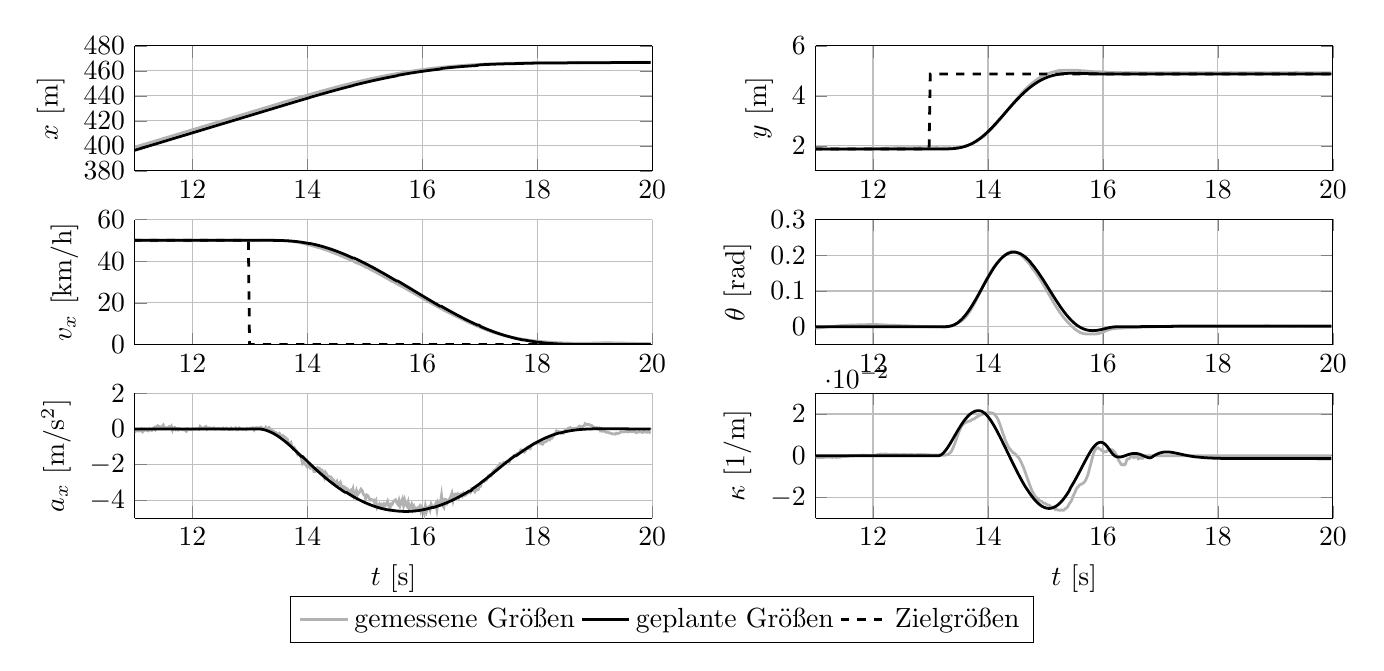
\begin{tikzpicture}

\begin{axis}[%
width=0.410625\figurewidth,
height=0.264706\figureheight,
at={(0.540296\figurewidth,0\figureheight)},
scale only axis,
separate axis lines,
every outer x axis line/.append style={black},
every x tick label/.append style={font=\color{black}},
xmin=11,
xmax=20,
xlabel={$t$ [s]},
xlabel near ticks,
xmajorgrids,
every outer y axis line/.append style={black},
every y tick label/.append style={font=\color{black}},
ymin=-0.03,
ymax=0.03,
ylabel near ticks,
ylabel={$\kappa\text{ [1/m]}$},
ymajorgrids
]
\addplot [color=light-gray,solid,forget plot,line width=1.0]
  table[row sep=crcr]{%
10.975	-0.0008\\
10.995	-0.0008\\
11.015	-0.0008\\
11.035	-0.0008\\
11.055	-0.0008\\
11.075	-0.0009\\
11.095	-0.0008\\
11.115	-0.0008\\
11.135	-0.0009\\
11.155	-0.0007\\
11.175	-0.0007\\
11.195	-0.0007\\
11.215	-0.0006\\
11.235	-0.0007\\
11.255	-0.0007\\
11.275	-0.0007\\
11.295	-0.0008\\
11.315	-0.0007\\
11.335	-0.0005\\
11.355	-0.0008\\
11.375	-0.0008\\
11.395	-0.0005\\
11.415	-0.0007\\
11.435	-0.0006\\
11.455	-0.0005\\
11.475	-0.0003\\
11.495	-0.0003\\
11.515	-0.0004\\
11.535	-0.0002\\
11.555	-0.0003\\
11.575	-0.0002\\
11.595	0\\
11.615	0\\
11.635	-0.0001\\
11.655	0\\
11.675	0\\
11.695	0.0001\\
11.715	0.0001\\
11.735	0\\
11.755	0.0001\\
11.775	0.0002\\
11.795	0.0001\\
11.815	0.0002\\
11.835	0.0003\\
11.855	0.0002\\
11.875	0.0002\\
11.895	0.0002\\
11.915	0.0001\\
11.935	0\\
11.955	0.0001\\
11.975	0.0001\\
11.995	0.0001\\
12.015	0.0001\\
12.035	0.0002\\
12.055	0.0003\\
12.075	0.0005\\
12.095	0.0006\\
12.115	0.0007\\
12.135	0.0008\\
12.155	0.0007\\
12.175	0.0007\\
12.195	0.0008\\
12.215	0.0008\\
12.235	0.0008\\
12.255	0.0007\\
12.275	0.0006\\
12.295	0.0006\\
12.315	0.0006\\
12.335	0.0005\\
12.355	0.0007\\
12.375	0.0007\\
12.395	0.0006\\
12.415	0.0006\\
12.435	0.0006\\
12.455	0.0005\\
12.475	0.0005\\
12.495	0.0006\\
12.515	0.0007\\
12.535	0.0005\\
12.555	0.0006\\
12.575	0.0006\\
12.595	0.0005\\
12.615	0.0005\\
12.635	0.0006\\
12.655	0.0005\\
12.675	0.0006\\
12.695	0.0005\\
12.715	0.0005\\
12.735	0.0005\\
12.755	0.0005\\
12.775	0.0006\\
12.795	0.0006\\
12.815	0.0005\\
12.835	0.0006\\
12.855	0.0005\\
12.875	0.0005\\
12.895	0.0006\\
12.915	0.0005\\
12.935	0.0004\\
12.955	0.0005\\
12.975	0.0005\\
12.995	0.0003\\
13.015	0.0004\\
13.035	0.0004\\
13.055	0.0004\\
13.075	0.0003\\
13.095	0.0003\\
13.115	0.0003\\
13.135	0.0003\\
13.155	0.0004\\
13.175	0.0003\\
13.195	0.0003\\
13.215	0.0002\\
13.235	0.0002\\
13.255	0.0003\\
13.275	0.0005\\
13.295	0.0005\\
13.315	0.0008\\
13.335	0.0013\\
13.355	0.0018\\
13.375	0.0027\\
13.395	0.004\\
13.415	0.0053\\
13.435	0.0068\\
13.455	0.0084\\
13.475	0.01\\
13.495	0.0114\\
13.515	0.0128\\
13.535	0.0139\\
13.555	0.0147\\
13.575	0.0153\\
13.595	0.0157\\
13.615	0.016\\
13.635	0.0162\\
13.655	0.0165\\
13.675	0.0166\\
13.695	0.0168\\
13.715	0.0172\\
13.735	0.0175\\
13.755	0.0176\\
13.775	0.018\\
13.795	0.0184\\
13.815	0.0188\\
13.835	0.019\\
13.855	0.0194\\
13.875	0.0196\\
13.895	0.0198\\
13.915	0.02\\
13.935	0.0202\\
13.955	0.0204\\
13.975	0.0206\\
13.995	0.0206\\
14.015	0.0208\\
14.035	0.0207\\
14.055	0.0205\\
14.075	0.0205\\
14.095	0.0203\\
14.115	0.0198\\
14.135	0.0191\\
14.155	0.0183\\
14.175	0.0174\\
14.195	0.0159\\
14.215	0.0145\\
14.235	0.0128\\
14.255	0.011\\
14.275	0.0096\\
14.295	0.0079\\
14.315	0.0066\\
14.335	0.0054\\
14.355	0.0042\\
14.375	0.0034\\
14.395	0.0028\\
14.415	0.0021\\
14.435	0.0015\\
14.455	0.0012\\
14.475	0.0008\\
14.495	0.0002\\
14.515	-0.0004\\
14.535	-0.001\\
14.555	-0.0019\\
14.575	-0.003\\
14.595	-0.0043\\
14.615	-0.0055\\
14.635	-0.0069\\
14.655	-0.0085\\
14.675	-0.01\\
14.695	-0.0116\\
14.715	-0.0132\\
14.735	-0.0147\\
14.755	-0.0161\\
14.775	-0.0173\\
14.795	-0.0183\\
14.815	-0.0193\\
14.835	-0.0198\\
14.855	-0.0204\\
14.875	-0.0208\\
14.895	-0.0215\\
14.915	-0.0217\\
14.935	-0.0219\\
14.955	-0.0225\\
14.975	-0.0228\\
14.995	-0.0228\\
15.015	-0.0233\\
15.035	-0.0236\\
15.055	-0.0236\\
15.075	-0.024\\
15.095	-0.0245\\
15.115	-0.0247\\
15.135	-0.0249\\
15.155	-0.0252\\
15.175	-0.0259\\
15.195	-0.0258\\
15.215	-0.026\\
15.235	-0.0262\\
15.255	-0.0262\\
15.275	-0.026\\
15.295	-0.0262\\
15.315	-0.0262\\
15.335	-0.0257\\
15.355	-0.0252\\
15.375	-0.0249\\
15.395	-0.0241\\
15.415	-0.023\\
15.435	-0.0223\\
15.455	-0.0214\\
15.475	-0.0197\\
15.495	-0.0186\\
15.515	-0.0175\\
15.535	-0.016\\
15.555	-0.0152\\
15.575	-0.0147\\
15.595	-0.014\\
15.615	-0.0137\\
15.635	-0.0135\\
15.655	-0.0132\\
15.675	-0.0126\\
15.695	-0.012\\
15.715	-0.0107\\
15.735	-0.0094\\
15.755	-0.0075\\
15.775	-0.0052\\
15.795	-0.0033\\
15.815	-0.0009\\
15.835	0.001\\
15.855	0.0023\\
15.875	0.0032\\
15.895	0.0038\\
15.915	0.0038\\
15.935	0.0034\\
15.955	0.0031\\
15.975	0.0026\\
15.995	0.0023\\
16.015	0.002\\
16.035	0.0018\\
16.055	0.0019\\
16.075	0.0024\\
16.095	0.0025\\
16.115	0.0024\\
16.135	0.0029\\
16.155	0.0029\\
16.175	0.0026\\
16.195	0.002\\
16.215	0.0012\\
16.235	0.0005\\
16.255	-0.001\\
16.275	-0.0024\\
16.295	-0.003\\
16.315	-0.0042\\
16.335	-0.0044\\
16.355	-0.0042\\
16.375	-0.0044\\
16.395	-0.0037\\
16.415	-0.0019\\
16.435	-0.0015\\
16.455	-0.0015\\
16.475	-0.0008\\
16.495	0.0002\\
16.515	-0.0003\\
16.535	-0.0009\\
16.555	-0.0007\\
16.575	-0.0004\\
16.595	-0.0004\\
16.615	-0.0015\\
16.635	-0.0012\\
16.655	-0.0006\\
16.675	-0.0012\\
16.695	-0.0012\\
16.715	0\\
16.735	0\\
16.755	0\\
16.775	0\\
16.795	0\\
16.815	0\\
16.835	0\\
16.855	0\\
16.875	0\\
16.895	0\\
16.915	0\\
16.935	0\\
16.955	0\\
16.975	0\\
16.995	0\\
17.015	0\\
17.035	0\\
17.055	0\\
17.075	0\\
17.095	0\\
17.115	0\\
17.135	0\\
17.155	0\\
17.175	0\\
17.195	0\\
17.215	0\\
17.235	0\\
17.255	0\\
17.275	0\\
17.295	0\\
17.315	0\\
17.335	0\\
17.355	0\\
17.375	0\\
17.395	0\\
17.415	0\\
17.435	0\\
17.455	0\\
17.475	0\\
17.495	0\\
17.515	0\\
17.535	0\\
17.555	0\\
17.575	0\\
17.595	0\\
17.615	0\\
17.635	0\\
17.655	0\\
17.675	0\\
17.695	0\\
17.715	0\\
17.735	0\\
17.755	0\\
17.775	0\\
17.795	0\\
17.815	0\\
17.835	0\\
17.855	0\\
17.875	0\\
17.895	0\\
17.915	0\\
17.935	0\\
17.955	0\\
17.975	0\\
17.995	0\\
18.015	0\\
18.035	0\\
18.055	0\\
18.075	0\\
18.095	0\\
18.115	0\\
18.135	0\\
18.155	0\\
18.175	0\\
18.195	0\\
18.215	0\\
18.235	0\\
18.255	0\\
18.275	0\\
18.295	0\\
18.315	0\\
18.335	0\\
18.355	0\\
18.375	0\\
18.395	0\\
18.415	0\\
18.435	0\\
18.455	0\\
18.475	0\\
18.495	0\\
18.515	0\\
18.535	0\\
18.555	0\\
18.575	0\\
18.595	0\\
18.615	0\\
18.635	0\\
18.655	0\\
18.675	0\\
18.695	0\\
18.715	0\\
18.735	0\\
18.755	0\\
18.775	0\\
18.795	0\\
18.815	0\\
18.835	0\\
18.855	0\\
18.875	0\\
18.895	0\\
18.915	0\\
18.935	0\\
18.955	0\\
18.975	0\\
18.995	0\\
19.015	0\\
19.035	0\\
19.055	0\\
19.075	0\\
19.095	0\\
19.115	0\\
19.135	0\\
19.155	0\\
19.175	0\\
19.195	0\\
19.215	0\\
19.235	0\\
19.255	0\\
19.275	0\\
19.295	0\\
19.315	0\\
19.335	0\\
19.355	0\\
19.375	0\\
19.395	0\\
19.415	0\\
19.435	0\\
19.455	0\\
19.475	0\\
19.495	0\\
19.515	0\\
19.535	0\\
19.555	0\\
19.575	0\\
19.595	0\\
19.615	0\\
19.635	0\\
19.655	0\\
19.675	0\\
19.695	0\\
19.715	0\\
19.735	0\\
19.755	0\\
19.775	0\\
19.795	0\\
19.815	0\\
19.835	0\\
19.855	0\\
19.875	0\\
19.895	0\\
19.915	0\\
19.935	0\\
19.955	0\\
19.975	0\\
};
\addplot [color=black,solid,forget plot, line width=1.0]
  table[row sep=crcr]{%
10.975	9.38148847495768e-009\\
10.995	9.45987199685305e-009\\
11.015	9.09139252769364e-009\\
11.035	8.36938784942731e-009\\
11.055	7.37805505579558e-009\\
11.075	6.19277695790288e-009\\
11.095	4.88053730762772e-009\\
11.115	3.50029649709427e-009\\
11.135	2.10335149297691e-009\\
11.155	7.33718696910302e-010\\
11.175	-5.7150401078232e-010\\
11.195	-1.78167269826446e-009\\
11.215	-2.87234236395761e-009\\
11.235	-3.82485643157793e-009\\
11.255	-4.62588234384498e-009\\
11.275	-5.26714361015479e-009\\
11.295	-5.74497738270452e-009\\
11.315	-6.05993655256043e-009\\
11.335	-6.21655527055509e-009\\
11.355	-6.22276630224405e-009\\
11.375	-6.089700299583e-009\\
11.395	-5.83114090346726e-009\\
11.415	-5.46328760009374e-009\\
11.435	-5.00431474037555e-009\\
11.455	-4.47412329407371e-009\\
11.475	-3.89363785657793e-009\\
11.495	-3.28475491251368e-009\\
11.515	-2.66987343344738e-009\\
11.535	-2.07136618968207e-009\\
11.555	-1.51148671356793e-009\\
11.575	-1.01163233345858e-009\\
11.595	-5.9256316520262e-010\\
11.615	-2.73234351810814e-010\\
11.635	-5.02802521840096e-011\\
11.655	1.0052545601491e-010\\
11.675	1.92129354092963e-010\\
11.695	2.36154013011358e-010\\
11.715	2.42959846685764e-010\\
11.735	2.21706972225455e-010\\
11.755	1.80417222828133e-010\\
11.775	1.26035973324612e-010\\
11.795	6.44934730620328e-011\\
11.815	7.68546847256663e-013\\
11.835	-6.10522535304803e-011\\
11.855	-1.17711299041368e-010\\
11.875	-1.66716279670354e-010\\
11.895	-2.06281686176979e-010\\
11.915	-2.35265029679965e-010\\
11.935	-2.53104648351155e-010\\
11.955	-2.59759103116153e-010\\
11.975	-2.5564203531836e-010\\
11.995	-2.41569431125299e-010\\
12.015	-2.18682585928498e-010\\
12.035	-1.88401946821237e-010\\
12.055	-1.52353199500688e-010\\
12.075	-1.12311389355302e-010\\
12.095	-7.01404004321837e-011\\
12.115	-2.77242812041223e-011\\
12.135	1.30846470811075e-011\\
12.155	5.05420427732162e-011\\
12.175	8.30556595721177e-011\\
12.195	1.09265513303924e-010\\
12.215	1.28075119953941e-010\\
12.235	1.3877214655178e-010\\
12.255	1.41022513111544e-010\\
12.275	1.34977709564943e-010\\
12.295	1.2130875470806e-010\\
12.315	1.01290115184227e-010\\
12.335	7.68618224622486e-011\\
12.355	5.06567392200008e-011\\
12.375	2.61007378904443e-011\\
12.395	7.09933414139163e-012\\
12.415	-5.93231236703518e-012\\
12.435	-1.4052081546978e-011\\
12.455	-1.8210407140562e-011\\
12.475	-1.92552605804419e-011\\
12.495	-1.79371465597322e-011\\
12.515	-1.49141619193438e-011\\
12.535	-1.07569066501445e-011\\
12.555	-5.95353800980636e-012\\
12.575	-9.148091355618e-013\\
12.595	4.02102916935432e-012\\
12.615	8.58317757146398e-012\\
12.635	1.25631883368671e-011\\
12.655	1.58100806751937e-011\\
12.675	1.82254870917387e-011\\
12.695	1.97582974287291e-011\\
12.715	2.03998033743158e-011\\
12.735	2.01786851117269e-011\\
12.755	1.91564975687841e-011\\
12.775	1.7421722051103e-011\\
12.795	1.50856653557963e-011\\
12.815	1.22766198248914e-011\\
12.835	9.13556209847233e-012\\
12.855	5.8112104538155e-012\\
12.875	2.45400639913018e-012\\
12.895	-7.87358839151459e-013\\
12.915	-3.7730495811017e-012\\
12.935	-6.37401893419098e-012\\
12.955	-8.4805764841156e-012\\
12.975	-1.00036420119798e-011\\
12.995	-1.088417984213e-011\\
13.015	-1.10936555081098e-011\\
13.035	-1.06421095893983e-011\\
13.055	-9.58222824004595e-012\\
13.075	-8.01295401559043e-012\\
13.095	-6.08831301346369e-012\\
13.115	-4.01692871673798e-012\\
13.135	-2.07200944769836e-012\\
13.155	7.61524279369041e-005\\
13.175	0.000294439669232816\\
13.195	0.000640104874037206\\
13.215	0.00109905668068677\\
13.235	0.00165786920115352\\
13.255	0.00230377702973783\\
13.275	0.00302466470748186\\
13.295	0.00380906090140343\\
13.315	0.00464611640200019\\
13.335	0.00552559411153197\\
13.355	0.00643784459680319\\
13.375	0.00737379351630807\\
13.395	0.00832490902394056\\
13.415	0.00928320270031691\\
13.435	0.010241175070405\\
13.455	0.0111918346956372\\
13.475	0.0121286436915398\\
13.495	0.0130455186590552\\
13.515	0.0139368204399943\\
13.535	0.0147973271086812\\
13.555	0.0156222078949213\\
13.575	0.0164070446044207\\
13.595	0.0171477943658829\\
13.615	0.017840787768364\\
13.635	0.0184827297925949\\
13.655	0.0190706793218851\\
13.675	0.0196020118892193\\
13.695	0.0200745072215796\\
13.715	0.0204862281680107\\
13.735	0.0208355896174908\\
13.755	0.0211213044822216\\
13.775	0.0213424079120159\\
13.795	0.0214982330799103\\
13.815	0.0215883702039719\\
13.835	0.0216127261519432\\
13.855	0.0215714070945978\\
13.875	0.0214648135006428\\
13.895	0.0212935190647841\\
13.915	0.0208893418312073\\
13.935	0.0205252654850483\\
13.955	0.0200681891292334\\
13.975	0.0195259526371956\\
13.995	0.0189060214906931\\
14.015	0.0182154532521963\\
14.035	0.0174609180539846\\
14.055	0.0166487339884043\\
14.075	0.0157848298549652\\
14.095	0.0148747498169541\\
14.115	0.0139237055554986\\
14.135	0.0129365483298898\\
14.155	0.0119178323075175\\
14.175	0.0108717568218708\\
14.195	0.0098022473976016\\
14.215	0.0087129594758153\\
14.235	0.00760728446766734\\
14.255	0.0064883790910244\\
14.275	0.00535917980596423\\
14.295	0.00422243913635612\\
14.315	0.00308071915060282\\
14.335	0.00193643930833787\\
14.355	0.0007918716291897\\
14.375	-0.000350823480403051\\
14.395	-0.00148959539365023\\
14.415	-0.00262247584760189\\
14.435	-0.00374756054952741\\
14.455	-0.0048630191013217\\
14.475	-0.00596705172210932\\
14.495	-0.00705791264772415\\
14.515	-0.00813384726643562\\
14.535	-0.00919315312057734\\
14.555	-0.0102341193705797\\
14.575	-0.0112550351768732\\
14.595	-0.012254199013114\\
14.615	-0.0132298897951841\\
14.635	-0.0141804125159979\\
14.655	-0.0151040479540825\\
14.675	-0.015894278883934\\
14.695	-0.0167499110102654\\
14.715	-0.0175765585154295\\
14.735	-0.0183720029890537\\
14.755	-0.0191340837627649\\
14.775	-0.0198606867343187\\
14.795	-0.020549725741148\\
14.815	-0.0211991760879755\\
14.835	-0.0218070726841688\\
14.855	-0.0223715417087078\\
14.875	-0.0228907614946365\\
14.895	-0.0233629811555147\\
14.915	-0.0237866062670946\\
14.935	-0.0241600964218378\\
14.955	-0.0244820471853018\\
14.975	-0.0247511677443981\\
14.995	-0.0249663032591343\\
15.015	-0.0251264497637749\\
15.035	-0.0252307299524546\\
15.055	-0.0252784211188555\\
15.075	-0.0252689998596907\\
15.095	-0.0252020508050919\\
15.115	-0.0250773653388023\\
15.135	-0.0248949136584997\\
15.155	-0.0246548224240541\\
15.175	-0.0243574250489473\\
15.195	-0.0240032058209181\\
15.215	-0.0235928744077683\\
15.235	-0.0231273099780083\\
15.255	-0.0226075984537601\\
15.275	-0.0220349989831448\\
15.295	-0.0214109793305397\\
15.315	-0.0207372177392244\\
15.335	-0.0200155545026064\\
15.355	-0.0192480850964785\\
15.375	-0.0184370670467615\\
15.395	-0.0175849869847298\\
15.415	-0.0166945457458496\\
15.435	-0.0154487006366253\\
15.455	-0.0145300589501858\\
15.475	-0.0135937612503767\\
15.495	-0.0126383891329169\\
15.515	-0.011663313023746\\
15.535	-0.010668683797121\\
15.555	-0.00965546444058418\\
15.575	-0.00862538628280163\\
15.595	-0.00758100813254714\\
15.615	-0.00652569532394409\\
15.635	-0.00546360807493329\\
15.655	-0.0043997117318213\\
15.675	-0.00333974603563547\\
15.695	-0.00229020859114826\\
15.715	-0.00125833577476442\\
15.735	-0.000252038182225078\\
15.755	0.000720137672033161\\
15.775	0.00164908799342811\\
15.795	0.00252524018287659\\
15.815	0.00333866570144892\\
15.835	0.00407921243458986\\
15.855	0.00473667168989778\\
15.875	0.00530098797753453\\
15.895	0.00576248578727245\\
15.915	0.00611215457320213\\
15.935	0.00634199054911733\\
15.955	0.00644539948552847\\
15.975	0.00641764560714364\\
15.995	0.00625641411170363\\
16.015	0.00596244959160686\\
16.035	0.00554029876366258\\
16.055	0.00499916216358542\\
16.075	0.00435391720384359\\
16.095	0.00362631003372371\\
16.115	0.00284624588675797\\
16.135	0.00205346406437457\\
16.155	0.00129925995133817\\
16.175	0.000648667337372899\\
16.195	0.000141284268465824\\
16.215	-0.00021642267529387\\
16.235	-0.000460295588709414\\
16.255	-0.000604157743509859\\
16.275	-0.000661558704450727\\
16.295	-0.000645733904093504\\
16.315	-0.000569559924770147\\
16.335	-0.000445504294475541\\
16.355	-0.000285565882222727\\
16.375	-0.000101219455245882\\
16.395	9.66589068411849e-005\\
16.415	0.00029786306549795\\
16.435	0.000492932158522308\\
16.455	0.000673242728225887\\
16.475	0.000831100915092975\\
16.495	0.000959834142122418\\
16.515	0.00105388753581792\\
16.535	0.00110893463715911\\
16.555	0.00112198665738106\\
16.575	0.00109147059265524\\
16.595	0.00101734348572791\\
16.615	0.000901181541848928\\
16.635	0.000746206089388579\\
16.655	0.000557409832254052\\
16.675	0.000341464794473723\\
16.695	0.000106784333183896\\
16.715	-0.00013668391329702\\
16.735	-0.000377511547412723\\
16.755	-0.000603243242949247\\
16.775	-0.000800598354544491\\
16.795	-0.000956356467213482\\
16.815	-0.00105803308542818\\
16.835	-0.00088266673265025\\
16.855	-0.000694614427629858\\
16.875	-0.000171450956258923\\
16.895	0.000124329992104322\\
16.915	0.000416566093917936\\
16.935	0.000693605747073889\\
16.955	0.000946863379795104\\
16.975	0.00117084791418165\\
16.995	0.00136221456341445\\
17.015	0.00151936302427202\\
17.035	0.00164265569765121\\
17.055	0.00173280166927725\\
17.075	0.00179165427107364\\
17.095	0.00182142097037286\\
17.115	0.00182470050640404\\
17.135	0.00180423317942768\\
17.155	0.00176282704342157\\
17.175	0.00170313054695725\\
17.195	0.00162822415586561\\
17.215	0.00154031591955572\\
17.235	0.00144191144499928\\
17.255	0.00133530143648386\\
17.275	0.00122233352158219\\
17.295	0.00110503996256739\\
17.315	0.000984836951829493\\
17.335	0.000862893648445606\\
17.355	0.000741032534278929\\
17.375	0.000619568105321378\\
17.395	0.000500011083204299\\
17.415	0.000383059930754825\\
17.435	0.00026850585709326\\
17.455	0.00015788254677318\\
17.475	5.05603638885077e-005\\
17.495	-5.21098299941514e-005\\
17.515	-0.000150760897668079\\
17.535	-0.000244750815909356\\
17.555	-0.000334092968842015\\
17.575	-0.000419403077103198\\
17.595	-0.000500212074257433\\
17.615	-0.000576465739868581\\
17.635	-0.000575385871343315\\
17.655	-0.00064448470948264\\
17.675	-0.000707569241058081\\
17.695	-0.00076569092925638\\
17.715	-0.000819005013909191\\
17.735	-0.000868120812810957\\
17.755	-0.000912855379283428\\
17.775	-0.000954058952629566\\
17.795	-0.000991941662505269\\
17.815	-0.00102669955231249\\
17.835	-0.00105864589568228\\
17.855	-0.00108768558129668\\
17.875	-0.00111473130527884\\
17.895	-0.00113939878065139\\
17.915	-0.0011621720623225\\
17.935	-0.00118291424587369\\
17.955	-0.00120184221304953\\
17.975	-0.00121960090473294\\
17.995	-0.00123547448311001\\
18.015	-0.00125019589904696\\
18.035	-0.00126339041162282\\
18.055	-0.00127584952861071\\
18.075	-0.00128708721604198\\
18.095	-0.00129735225345939\\
18.115	-0.0013067782856524\\
18.135	-0.00131519662681967\\
18.155	-0.00132293126080185\\
18.175	-0.00133029115386307\\
18.195	-0.00133671355433762\\
18.215	-0.00134250754490495\\
18.235	-0.00134759407956153\\
18.255	-0.00135236175265163\\
18.275	-0.00135672418400645\\
18.295	-0.00136059720534831\\
18.315	-0.00136417197063565\\
18.335	-0.00136708980426192\\
18.355	-0.0013699937844649\\
18.375	-0.0013724333839491\\
18.395	-0.00137243268545717\\
18.415	-0.00137459125835449\\
18.435	-0.00137656240258366\\
18.455	-0.001378258690238\\
18.475	-0.00137968303170055\\
18.495	-0.00138092611450702\\
18.515	-0.00138216628693044\\
18.535	-0.00138305022846907\\
18.555	-0.00138375617098063\\
18.575	-0.00138437317218632\\
18.595	-0.00138507748488337\\
18.615	-0.00138534139841795\\
18.635	-0.00138569297268987\\
18.655	-0.00138604443054646\\
18.675	-0.00138613232411444\\
18.695	-0.00138630776200444\\
18.715	-0.00138630776200444\\
18.735	-0.00138630776200444\\
18.755	-0.00138621998485178\\
18.775	-0.00138613232411444\\
18.795	-0.00138613232411444\\
18.815	-0.00138604443054646\\
18.835	-0.0013858686434105\\
18.855	-0.00138560507912189\\
18.875	-0.00138542940840125\\
18.895	-0.00138534139841795\\
18.915	-0.00138516549486667\\
18.935	-0.00138490158133209\\
18.955	-0.00138481345493346\\
18.975	-0.00138472556136549\\
18.995	-0.00138428504578769\\
19.015	-0.00138419691938907\\
19.035	-0.0013839325401932\\
19.055	-0.00138375617098063\\
19.075	-0.00138366792816669\\
19.095	-0.00138366792816669\\
19.115	-0.0013834914425388\\
19.135	-0.00138322694692761\\
19.155	-0.0013834914425388\\
19.175	-0.0013834914425388\\
19.195	-0.00138357968535274\\
19.215	-0.00138357968535274\\
19.235	-0.00138366792816669\\
19.255	-0.00138366792816669\\
19.275	-0.00138375605456531\\
19.295	-0.00138384429737926\\
19.315	-0.00138393242377788\\
19.335	-0.00138402066659182\\
19.355	-0.00138402066659182\\
19.375	-0.00138428504578769\\
19.395	-0.00138437328860164\\
19.415	-0.00138454942498356\\
19.435	-0.00138463743496686\\
19.455	-0.00138481345493346\\
19.475	-0.00138507748488337\\
19.495	-0.00138516549486667\\
19.515	-0.00138525338843465\\
19.535	-0.00138551718555391\\
19.555	-0.00138569285627455\\
19.575	-0.00138578074984252\\
19.595	-0.00138595653697848\\
19.615	-0.00138621998485178\\
19.635	-0.00138648319989443\\
19.655	-0.00138648319989443\\
19.675	-0.00138674629852176\\
19.695	-0.00138692161999643\\
19.715	-0.00138718460220844\\
19.735	-0.0013874473515898\\
19.755	-0.0013874473515898\\
19.775	-0.00138771010097116\\
19.795	-0.00138788507319987\\
19.815	-0.00138806004542857\\
19.835	-0.00138814747333527\\
19.855	-0.00138840975705534\\
19.875	-0.00138849706854671\\
19.895	-0.00138875923585147\\
19.915	-0.00138867180794477\\
19.935	-0.00138884654734284\\
19.955	-0.00138902117032558\\
19.975	-0.001389195676893\\
};
\end{axis}

\begin{axis}[%
width=0.410625\figurewidth,
height=0.264706\figureheight,
at={(0.540296\figurewidth,0.367647\figureheight)},
scale only axis,
separate axis lines,
every outer x axis line/.append style={black},
every x tick label/.append style={font=\color{black}},
xmin=11,
xmax=20,
xmajorgrids,
every outer y axis line/.append style={black},
every y tick label/.append style={font=\color{black}},
ymin=-0.05,
ymax=0.3,
ylabel={$\theta{}\text{ [rad]}$},
ylabel near ticks,
ymajorgrids
]
\addplot [color=light-gray,solid,forget plot,line width=1.0]
  table[row sep=crcr]{%
10.975	-0.00483439303934574\\
10.995	-0.00451913895085454\\
11.015	-0.00403015315532684\\
11.035	-0.00371382758021355\\
11.055	-0.00340464920736849\\
11.075	-0.0031281728297472\\
11.095	-0.00268081738613546\\
11.115	-0.00234167650341988\\
11.135	-0.00200298940762877\\
11.155	-0.00164385139942169\\
11.175	-0.00127162481658161\\
11.195	-0.000931398419197649\\
11.215	-0.000425654667196795\\
11.235	-0.00014473038027063\\
11.255	9.24975829548202e-005\\
11.275	0.00036603314219974\\
11.295	0.00071013969136402\\
11.315	0.0010577297070995\\
11.335	0.00139422703068703\\
11.355	0.0017333080759272\\
11.375	0.00219001923687756\\
11.395	0.0022976640611887\\
11.415	0.00261506601236761\\
11.435	0.00293107074685395\\
11.455	0.00319629046134651\\
11.475	0.00344069371931255\\
11.495	0.00352165382355452\\
11.515	0.00377931469120085\\
11.535	0.0038671309594065\\
11.555	0.0039545614272356\\
11.575	0.00424557365477085\\
11.595	0.00440585799515247\\
11.615	0.00455497624352574\\
11.635	0.00463511003181338\\
11.655	0.00471678376197815\\
11.675	0.00477723404765129\\
11.695	0.00483727781102061\\
11.715	0.00499625317752361\\
11.735	0.00516080670058727\\
11.755	0.00527735473588109\\
11.775	0.00537290750071406\\
11.795	0.00534263486042619\\
11.815	0.00550834601745009\\
11.835	0.00563527410849929\\
11.855	0.00553830340504646\\
11.875	0.0056325402110815\\
11.895	0.00574886985123158\\
11.915	0.0058641224168241\\
11.935	0.00595522578805685\\
11.955	0.00587058207020164\\
11.975	0.00590058974921703\\
11.995	0.00593192968517542\\
12.015	0.005979357752949\\
12.035	0.00602993601933122\\
12.055	0.00606499426066875\\
12.075	0.00592184765264392\\
12.095	0.00575958611443639\\
12.115	0.00558505300432444\\
12.135	0.00542569765821099\\
12.155	0.00528155546635389\\
12.175	0.00514543056488037\\
12.195	0.00502065755426884\\
12.215	0.00471238838508725\\
12.235	0.00453785574063659\\
12.255	0.00436954759061337\\
12.275	0.00427515711635351\\
12.295	0.00418374128639698\\
12.315	0.00401425687596202\\
12.335	0.00401425687596202\\
12.355	0.00372830522246659\\
12.375	0.00381141202524304\\
12.395	0.0036651911213994\\
12.415	0.00349065847694874\\
12.435	0.00333178066648543\\
12.455	0.0031892757397145\\
12.475	0.00305238901637495\\
12.495	0.00292894314043224\\
12.515	0.00296705961227417\\
12.535	0.00279252673499286\\
12.555	0.00262482278048992\\
12.575	0.0025304276496172\\
12.595	0.00243900623172522\\
12.615	0.00226892810314894\\
12.635	0.00209439499303699\\
12.655	0.00191986211575568\\
12.675	0.00191986211575568\\
12.695	0.00174532923847437\\
12.715	0.00157079636119306\\
12.735	0.00139626336749643\\
12.755	0.00122173049021512\\
12.775	0.0012336039217189\\
12.795	0.00109147350303829\\
12.815	0.000952567032072693\\
12.835	0.000828756135888398\\
12.855	0.000701412267517298\\
12.875	0.000735987967345864\\
12.895	0.000594562268815935\\
12.915	0.000468334998004138\\
12.935	0.000340828002663329\\
12.955	0.000349065900081769\\
12.975	0.000174532979144715\\
12.995	5.48260068171658e-005\\
13.015	0.000137932162033394\\
13.035	4.30011061480773e-011\\
13.055	3.78349990226567e-011\\
13.075	-0.000150637730257586\\
13.095	-8.89875518623739e-005\\
13.115	-0.000214108091313392\\
13.135	-0.000192654260899872\\
13.155	-0.000349065841874108\\
13.175	-0.000349065841874108\\
13.195	-0.000523598748259246\\
13.215	-0.000523598748259246\\
13.235	-0.000509376986883581\\
13.255	-0.000638434430584311\\
13.275	-0.00044242013245821\\
13.295	-0.000214132131077349\\
13.315	0.000294335419312119\\
13.335	0.000916192075237632\\
13.355	0.0018915687687695\\
13.375	0.00297170225530863\\
13.395	0.00420343596488237\\
13.415	0.00571291660889983\\
13.435	0.00715364469215274\\
13.455	0.00875583384186029\\
13.475	0.0103405928239226\\
13.495	0.012110099196434\\
13.515	0.0138591974973679\\
13.535	0.0159659888595343\\
13.555	0.0184932127594948\\
13.575	0.0211956650018692\\
13.595	0.024395115673542\\
13.615	0.0280760042369366\\
13.635	0.0320195220410824\\
13.655	0.0362177491188049\\
13.675	0.0410008020699024\\
13.695	0.0459900014102459\\
13.715	0.0513581037521362\\
13.735	0.0569324344396591\\
13.755	0.0629786103963852\\
13.775	0.0689269378781319\\
13.795	0.0751102790236473\\
13.815	0.0814620926976204\\
13.835	0.08797487616539\\
13.855	0.0944609865546227\\
13.875	0.101039662957191\\
13.895	0.107544586062431\\
13.915	0.114099718630314\\
13.935	0.120607577264309\\
13.955	0.127007782459259\\
13.975	0.133139878511429\\
13.995	0.138508960604668\\
14.015	0.144446417689323\\
14.035	0.14996574819088\\
14.055	0.155373007059097\\
14.075	0.160490453243256\\
14.095	0.165264219045639\\
14.115	0.169773995876312\\
14.135	0.173960700631142\\
14.155	0.177855342626572\\
14.175	0.181625500321388\\
14.195	0.185052931308746\\
14.215	0.188465446233749\\
14.235	0.191673189401627\\
14.255	0.194837927818298\\
14.275	0.197772860527039\\
14.295	0.200471863150597\\
14.315	0.203103393316269\\
14.335	0.205316424369812\\
14.355	0.207117453217506\\
14.375	0.208682402968407\\
14.395	0.209825798869133\\
14.415	0.210565850138664\\
14.435	0.210889026522636\\
14.455	0.210599526762962\\
14.475	0.209887966513634\\
14.495	0.208614647388458\\
14.515	0.207015544176102\\
14.535	0.205214142799377\\
14.555	0.202833577990532\\
14.575	0.200071692466736\\
14.595	0.197319120168686\\
14.615	0.194094255566597\\
14.635	0.190908581018448\\
14.655	0.187416553497314\\
14.675	0.183977425098419\\
14.695	0.180281788110733\\
14.715	0.176548466086388\\
14.735	0.172778606414795\\
14.755	0.166822656989098\\
14.775	0.162805020809174\\
14.795	0.158624708652496\\
14.815	0.154465854167938\\
14.835	0.150020197033882\\
14.855	0.145302042365074\\
14.875	0.140546351671219\\
14.895	0.135574862360954\\
14.915	0.130569651722908\\
14.935	0.125341147184372\\
14.955	0.119939461350441\\
14.975	0.114401087164879\\
14.995	0.108973294496536\\
15.015	0.103290572762489\\
15.035	0.0977189987897873\\
15.055	0.0919091105461121\\
15.075	0.0862571224570274\\
15.095	0.0806166529655457\\
15.115	0.0750076100230217\\
15.135	0.0694537907838821\\
15.155	0.0641543194651604\\
15.175	0.0588194951415062\\
15.195	0.0537868142127991\\
15.215	0.0487291887402534\\
15.235	0.0438425615429878\\
15.255	0.0391476228833199\\
15.275	0.0346642807126045\\
15.295	0.0304115638136864\\
15.315	0.0262331068515778\\
15.335	0.0223206169903278\\
15.355	0.0185136273503304\\
15.375	0.0149959102272987\\
15.395	0.0114402994513512\\
15.415	0.00803345441818237\\
15.435	0.00493914633989334\\
15.455	0.00183527916669846\\
15.475	-0.00108802318572998\\
15.495	-0.0039878822863102\\
15.515	-0.00684348307549953\\
15.535	-0.00927583687007427\\
15.555	-0.0115190958604217\\
15.575	-0.0135813420638442\\
15.595	-0.0154619161039591\\
15.615	-0.0169806070625782\\
15.635	-0.0181384738534689\\
15.655	-0.0190950985997915\\
15.675	-0.0196885839104652\\
15.695	-0.0201043952256441\\
15.715	-0.0203469023108482\\
15.735	-0.0204577334225178\\
15.755	-0.0205946899950504\\
15.775	-0.0205855667591095\\
15.795	-0.0206108465790749\\
15.815	-0.0206425711512566\\
15.835	-0.0207072347402573\\
15.855	-0.0205147508531809\\
15.875	-0.020250340923667\\
15.895	-0.0199508983641863\\
15.915	-0.0194827634841204\\
15.935	-0.0186694879084826\\
15.955	-0.0177136063575745\\
15.975	-0.0166447069495916\\
15.995	-0.0154935643076897\\
16.015	-0.0141174532473087\\
16.035	-0.0128977093845606\\
16.055	-0.0115175386890769\\
16.075	-0.0101832151412964\\
16.095	-0.00909971352666616\\
16.115	-0.00794643722474575\\
16.135	-0.00709790922701359\\
16.155	-0.00640112720429897\\
16.175	-0.00569774629548192\\
16.195	-0.00534668657928705\\
16.215	-0.00483251176774502\\
16.235	-0.00466508185490966\\
16.255	-0.00464842421934009\\
16.275	-0.00440300488844514\\
16.295	-0.00406999187543988\\
16.315	-0.00397666776552796\\
16.335	-0.00375404581427574\\
16.355	-0.00354636879637837\\
16.375	-0.00334203150123358\\
16.395	-0.00312494090758264\\
16.415	-0.00306154508143663\\
16.435	-0.00297144637443125\\
16.455	-0.00284127844497561\\
16.475	-0.00284184189513326\\
16.495	-0.00280879624187946\\
16.515	-0.0027437093667686\\
16.535	-0.00247504422441125\\
16.555	-0.00235604192130268\\
16.575	-0.0022172552999109\\
16.595	-0.00206443434581161\\
16.615	-0.00172920909244567\\
16.635	-0.00156700145453215\\
16.655	-0.00140952889341861\\
16.675	-0.00108825869392604\\
16.695	-0.000957716139964759\\
16.715	-0.000673596689011902\\
16.735	-0.00058883655583486\\
16.755	-0.000531715981196612\\
16.775	-0.000503859599120915\\
16.795	-0.000505547621287405\\
16.815	-0.000505547621287405\\
16.835	-0.000417621631640941\\
16.855	-0.000496391323395073\\
16.875	-0.000417910632677376\\
16.895	-0.000525287061464041\\
16.915	-8.07306496426463e-005\\
16.935	1.14298309199512e-005\\
16.955	9.65120852924883e-005\\
16.975	0.00026870277361013\\
16.995	0.000293723860522732\\
17.015	0.000518253014888614\\
17.035	0.000590036390349269\\
17.055	0.000680043362081051\\
17.075	0.000784516043495387\\
17.095	0.000899647304322571\\
17.115	0.00102229556068778\\
17.135	0.0013236126396805\\
17.155	0.00145188614260405\\
17.175	0.00157917651813477\\
17.195	0.00170338503085077\\
17.215	0.00182311749085784\\
17.235	0.00193687668070197\\
17.255	0.00204391032457352\\
17.275	0.0021429134067148\\
17.295	0.00223397486843169\\
17.315	0.00231667188927531\\
17.335	0.00239088176749647\\
17.355	0.00245679961517453\\
17.375	0.00251450552605093\\
17.395	0.00256440578959882\\
17.415	0.00243241246789694\\
17.435	0.00246781785972416\\
17.455	0.00249677244573832\\
17.475	0.00251960474997759\\
17.495	0.00253686006180942\\
17.515	0.00272366707213223\\
17.535	0.00273133371956646\\
17.555	0.00273494375869632\\
17.575	0.00256038340739906\\
17.595	0.00255717989057302\\
17.615	0.00255121383816004\\
17.635	0.00254289503209293\\
17.655	0.00253250193782151\\
17.675	0.00252040289342403\\
17.695	0.00250693154521286\\
17.715	0.00250693899579346\\
17.735	0.0026669108774513\\
17.755	0.00265163998119533\\
17.775	0.00263576535508037\\
17.795	0.00261956127360463\\
17.815	0.00260313437320292\\
17.835	0.00258682668209076\\
17.855	0.00257058744318783\\
17.875	0.00255455123260617\\
17.895	0.00253884098492563\\
17.915	0.00269803544506431\\
17.935	0.00268329726532102\\
17.955	0.00266884570010006\\
17.975	0.00265501835383475\\
17.995	0.00281620514579117\\
18.015	0.0028035375289619\\
18.035	0.00279152928851545\\
18.055	0.00277985306456685\\
18.075	0.00276906392537057\\
18.095	0.00275874719955027\\
18.115	0.00274923513643444\\
18.135	0.00274001387879252\\
18.155	0.00273148808628321\\
18.175	0.00272352178581059\\
18.195	0.00289058452472091\\
18.215	0.00288378307595849\\
18.235	0.00287742260843515\\
18.255	0.00287126936018467\\
18.275	0.00286581553518772\\
18.295	0.00286082830280066\\
18.315	0.00285639520734549\\
18.335	0.00285219307988882\\
18.355	0.00284830760210752\\
18.375	0.00284482445567846\\
18.395	0.00284158159047365\\
18.415	0.00283891428261995\\
18.435	0.00283624138683081\\
18.455	0.00283398199826479\\
18.475	0.0028339815326035\\
18.495	0.00283196941018105\\
18.515	0.00283012259751558\\
18.535	0.00282852537930012\\
18.555	0.00282717868685722\\
18.575	0.00282599870115519\\
18.595	0.00282481871545315\\
18.615	0.00282397447153926\\
18.635	0.00282329926267266\\
18.655	0.00282270787283778\\
18.675	0.00282203173264861\\
18.695	0.00282177794724703\\
18.715	0.00282143987715244\\
18.735	0.00282110134139657\\
18.755	0.00282101659104228\\
18.775	0.00282084755599499\\
18.795	0.00282084755599499\\
18.815	0.00299538066610694\\
18.835	0.00299546518363059\\
18.855	0.00299554970115423\\
18.875	0.00299554970115423\\
18.895	0.00299563445150852\\
18.915	0.00282127084210515\\
18.935	0.00282152462750673\\
18.955	0.00264716031961143\\
18.975	0.00247271219268441\\
18.995	0.0024728812277317\\
19.015	0.00247313478030264\\
19.035	0.00247321929782629\\
19.055	0.00247330381534994\\
19.075	0.00247372640296817\\
19.095	0.00247381092049181\\
19.115	0.00247406447306275\\
19.135	0.0024742332752794\\
19.155	0.00247431755997241\\
19.175	0.00247431755997241\\
19.195	0.00247448636218905\\
19.215	0.00230020703747869\\
19.235	0.00229995348490775\\
19.255	0.00229995348490775\\
19.275	0.0022998689673841\\
19.295	0.0022998689673841\\
19.315	0.0022997846826911\\
19.335	0.0022997846826911\\
19.355	0.00247423304244876\\
19.375	0.00247414852492511\\
19.395	0.00247406424023211\\
19.415	0.00247397972270846\\
19.435	0.00247397972270846\\
19.455	0.00247372617013752\\
19.475	0.00247364165261388\\
19.495	0.00229893974028528\\
19.515	0.00229885522276163\\
19.535	0.00229868618771434\\
19.555	0.0022984326351434\\
19.575	0.00229834811761975\\
19.595	0.00229826360009611\\
19.615	0.00229800981469452\\
19.635	0.00229784077964723\\
19.655	0.00229775602929294\\
19.675	0.00229758699424565\\
19.695	0.00229733320884407\\
19.715	0.00229707942344248\\
19.735	0.00229707942344248\\
19.755	0.00229682540521026\\
19.775	0.00229665613733232\\
19.795	0.00229640235193074\\
19.815	0.00229614833369851\\
19.835	0.00229614833369851\\
19.855	0.00229589408263564\\
19.875	0.00229572458192706\\
19.895	0.00229555531404912\\
19.915	0.00229547056369483\\
19.935	0.00229521631263196\\
19.955	0.00229513156227767\\
19.975	0.0022948773112148\\
};
\addplot [color=black,solid,forget plot, line width=1.0]
  table[row sep=crcr]{%
10.975	3.46754680524697e-010\\
10.995	1.44974465765557e-009\\
11.015	3.25399618361644e-009\\
11.035	5.52293144551186e-009\\
11.055	8.05564681627402e-009\\
11.075	1.06839941338421e-008\\
11.095	1.32697790533598e-008\\
11.115	1.57020636493144e-008\\
11.135	1.78945285256304e-008\\
11.155	1.97830427595136e-008\\
11.175	2.13232258516882e-008\\
11.195	2.24881766541785e-008\\
11.215	2.32663115440346e-008\\
11.235	2.36592594404783e-008\\
11.255	2.36799291286616e-008\\
11.275	2.33505907942799e-008\\
11.295	2.27011582865089e-008\\
11.315	2.17676365821262e-008\\
11.335	2.05902832561833e-008\\
11.355	1.92125071407645e-008\\
11.375	1.76792820383298e-008\\
11.395	1.60359672207733e-008\\
11.415	1.43272664843153e-008\\
11.435	1.25962005270708e-008\\
11.455	1.08831512690699e-008\\
11.475	9.22468057495962e-009\\
11.495	7.6536554871609e-009\\
11.515	6.19784623623332e-009\\
11.535	4.88015716726409e-009\\
11.555	3.71706554425089e-009\\
11.575	2.71956723807421e-009\\
11.595	1.89264603989159e-009\\
11.615	1.23470134116843e-009\\
11.635	7.38190231164282e-010\\
11.655	3.89295401470591e-010\\
11.675	1.68577152237503e-010\\
11.695	5.10353877214431e-011\\
11.715	7.93279504585076e-012\\
11.735	1.64258051604804e-011\\
11.755	5.83026960043753e-011\\
11.775	1.18762763512414e-010\\
11.795	1.86056850481897e-010\\
11.815	2.5114593737996e-010\\
11.835	3.07375541686028e-010\\
11.855	3.50168588569844e-010\\
11.875	3.76735420637431e-010\\
11.895	3.85799170388168e-010\\
11.915	3.77341241586393e-010\\
11.935	3.52361889666142e-010\\
11.955	3.12657011392048e-010\\
11.975	2.60617555314369e-010\\
11.995	1.99038258097417e-010\\
12.015	1.30949889820542e-010\\
12.035	5.94634411155148e-011\\
12.055	-1.23633872237128e-011\\
12.075	-8.16371692469176e-011\\
12.095	-1.45750370106335e-010\\
12.115	-2.02443811714303e-010\\
12.135	-2.4988178193297e-010\\
12.155	-2.86711460129041e-010\\
12.175	-3.12079195818882e-010\\
12.195	-3.25653642940793e-010\\
12.215	-3.27625898632888e-010\\
12.235	-3.18698512025151e-010\\
12.255	-3.00009989073757e-010\\
12.275	-2.73145311924239e-010\\
12.295	-2.39982533845051e-010\\
12.315	-2.02728653309059e-010\\
12.335	-1.63673977149337e-010\\
12.355	-1.25157662012043e-010\\
12.375	-8.93987106564964e-011\\
12.395	-5.83528503295128e-011\\
12.415	-3.35415480112733e-011\\
12.435	-1.58179771364564e-011\\
12.455	-5.22792789961479e-012\\
12.475	-7.68054511050137e-013\\
12.495	-7.31446207855729e-013\\
12.515	-3.60931206797033e-012\\
12.535	-8.17167600947188e-012\\
12.555	-1.34382192873428e-011\\
12.575	-1.8650530772546e-011\\
12.595	-2.32457161158939e-011\\
12.615	-2.68314103574196e-011\\
12.635	-2.91621934933595e-011\\
12.655	-3.01173391781262e-011\\
12.675	-2.96801160037941e-011\\
12.695	-2.79182683915469e-011\\
12.715	-2.49658054646273e-011\\
12.735	-2.10067414851967e-011\\
12.755	-1.62595631403306e-011\\
12.775	-1.09634142042569e-011\\
12.795	-5.36542685281027e-012\\
12.815	2.89968759724021e-013\\
12.835	5.77073762039748e-012\\
12.855	1.08663061187952e-011\\
12.875	1.5393767857641e-011\\
12.895	1.92034669416197e-011\\
12.915	2.21832621716267e-011\\
12.935	2.42616968182396e-011\\
12.955	2.54090689461028e-011\\
12.975	2.5635727915474e-011\\
12.995	2.49952870901016e-011\\
13.015	2.35754263333554e-011\\
13.035	2.15005530740386e-011\\
13.055	1.89174995113284e-011\\
13.075	1.60011257716031e-011\\
13.095	1.29337599658053e-011\\
13.115	9.90005386697357e-012\\
13.135	7.07806426317181e-012\\
13.155	4.62441239815203e-012\\
13.175	2.66072363794279e-012\\
13.195	1.25568284069233e-012\\
13.215	4.15522949165012e-013\\
13.235	7.11089478500071e-006\\
13.255	5.54653197468724e-005\\
13.275	0.000182478921487927\\
13.295	0.000421557226218283\\
13.315	0.000802277296315879\\
13.335	0.00135056767612696\\
13.355	0.00208888668566942\\
13.375	0.00303639750927687\\
13.395	0.00420913891866803\\
13.415	0.00562019506469369\\
13.435	0.00727985799312592\\
13.455	0.0091957887634635\\
13.475	0.0113731659948826\\
13.495	0.013814851641655\\
13.515	0.0165215060114861\\
13.535	0.0194917637854815\\
13.555	0.0227223467081785\\
13.575	0.0262081921100616\\
13.595	0.029942600056529\\
13.615	0.033917348831892\\
13.635	0.0381227880716324\\
13.655	0.0425479970872402\\
13.675	0.047180887311697\\
13.695	0.0520082786679268\\
13.715	0.0570160485804081\\
13.735	0.0621892027556896\\
13.755	0.0675120204687119\\
13.775	0.0729681327939034\\
13.795	0.0785406082868576\\
13.815	0.084212027490139\\
13.835	0.0899646505713463\\
13.855	0.0957804247736931\\
13.875	0.101641118526459\\
13.895	0.107528433203697\\
13.915	0.113423995673656\\
13.935	0.119309455156326\\
13.955	0.125166684389114\\
13.975	0.130977541208267\\
13.995	0.136406496167183\\
14.015	0.142031162977219\\
14.035	0.147535338997841\\
14.055	0.152894884347916\\
14.075	0.15808779001236\\
14.095	0.163094058632851\\
14.115	0.167895764112473\\
14.135	0.172476902604103\\
14.155	0.17682321369648\\
14.175	0.180922091007233\\
14.195	0.184762582182884\\
14.215	0.18833515048027\\
14.235	0.191631868481636\\
14.255	0.194645926356316\\
14.275	0.19737184047699\\
14.295	0.19980525970459\\
14.315	0.201943024992943\\
14.335	0.20378290116787\\
14.355	0.205323666334152\\
14.375	0.206564962863922\\
14.395	0.207507327198982\\
14.415	0.208152055740356\\
14.435	0.208501085639\\
14.455	0.208557337522507\\
14.475	0.208324044942856\\
14.495	0.207805350422859\\
14.515	0.207005798816681\\
14.535	0.205930560827255\\
14.555	0.204585358500481\\
14.575	0.20297634601593\\
14.595	0.201110184192657\\
14.615	0.198994070291519\\
14.635	0.196635484695435\\
14.655	0.194042444229126\\
14.675	0.191223278641701\\
14.695	0.188186764717102\\
14.715	0.184941962361336\\
14.735	0.18149833381176\\
14.755	0.176788702607155\\
14.775	0.17297925055027\\
14.795	0.169001191854477\\
14.815	0.164864420890808\\
14.835	0.160579264163971\\
14.855	0.156156376004219\\
14.875	0.151606753468513\\
14.895	0.146941632032394\\
14.915	0.14217247068882\\
14.935	0.137311056256294\\
14.955	0.132369220256805\\
14.975	0.127359047532082\\
14.995	0.122292689979076\\
15.015	0.117182396352291\\
15.035	0.112040415406227\\
15.055	0.106879092752934\\
15.075	0.101710684597492\\
15.095	0.0965473502874374\\
15.115	0.091401219367981\\
15.135	0.0862842500209808\\
15.155	0.0812081769108772\\
15.175	0.0761845707893372\\
15.195	0.0712247714400291\\
15.215	0.0663397610187531\\
15.235	0.0615402534604073\\
15.255	0.0568365901708603\\
15.275	0.0522387251257896\\
15.295	0.0477561727166176\\
15.315	0.0433980152010918\\
15.335	0.0391728430986404\\
15.355	0.035088736563921\\
15.375	0.0311532374471426\\
15.395	0.0273733232170343\\
15.415	0.0237553585320711\\
15.435	0.0203051194548607\\
15.455	0.0170277412980795\\
15.475	0.0139276962727308\\
15.495	0.0110087618231773\\
15.515	0.0081846984103322\\
15.535	0.00565952435135841\\
15.555	0.00331616448238492\\
15.575	0.00115431612357497\\
15.595	-0.000826266419608146\\
15.615	-0.00262590730562806\\
15.635	-0.00424513639882207\\
15.655	-0.00568480882793665\\
15.675	-0.00694622006267309\\
15.695	-0.00803122390061617\\
15.715	-0.00894230883568525\\
15.735	-0.00968271773308516\\
15.755	-0.0102565139532089\\
15.775	-0.0106686530634761\\
15.795	-0.0109250554814935\\
15.815	-0.0110326334834099\\
15.835	-0.0109993601217866\\
15.855	-0.0108342589810491\\
15.875	-0.0105474162846804\\
15.895	-0.0101499818265438\\
15.915	-0.00965411495417356\\
15.935	-0.00907294452190399\\
15.955	-0.00842047110199928\\
15.975	-0.00771148782223463\\
15.995	-0.00696138385683298\\
16.015	-0.00618606200441718\\
16.035	-0.00540165742859244\\
16.055	-0.00462430529296398\\
16.075	-0.00386987696401775\\
16.095	-0.00315359351225197\\
16.115	-0.00248968880623579\\
16.135	-0.00189089181367308\\
16.155	-0.00136796792503446\\
16.175	-0.0009290108573623\\
16.195	-0.000578948180191219\\
16.215	-0.000318634876748547\\
16.235	-0.000143963086884469\\
16.255	-4.50333936896641e-005\\
16.275	-5.89983619647683e-006\\
16.295	-1.06570314528653e-005\\
16.315	-4.50731531600468e-005\\
16.335	-9.76831361185759e-005\\
16.355	-0.000158896058565006\\
16.375	-0.000220867965254001\\
16.395	-0.000277374056167901\\
16.415	-0.00032368052052334\\
16.435	-0.000356416014255956\\
16.455	-0.000373441784176975\\
16.475	-0.000373723421944305\\
16.495	-0.0003572006826289\\
16.515	-0.000324657128658146\\
16.535	-0.000277590937912464\\
16.555	-0.000218089873669669\\
16.575	-0.000148696504766122\\
16.595	-7.22860640962608e-005\\
16.615	8.06006573839113e-006\\
16.635	8.91638774191961e-005\\
16.655	0.000167900157975964\\
16.675	0.000241268819081597\\
16.695	0.000306540110614151\\
16.715	0.000361333339242265\\
16.735	0.000403713405830786\\
16.755	0.000432273693149909\\
16.775	0.000446201884187758\\
16.795	0.000445357873104513\\
16.815	0.000445357873104513\\
16.835	0.000402054429287091\\
16.855	0.000362669583410025\\
16.875	0.000314643431920558\\
16.895	0.000260955217527226\\
16.915	0.000395966984797269\\
16.935	0.000354780757334083\\
16.955	0.000310055416775867\\
16.975	0.000308884307742119\\
16.995	0.00032139485119842\\
17.015	0.000346392975188792\\
17.035	0.000382284662919119\\
17.055	0.00042728814878501\\
17.075	0.000479524489492178\\
17.095	0.00053709011990577\\
17.115	0.000598414218984544\\
17.135	0.000661806319840252\\
17.155	0.000725943071302027\\
17.175	0.000789588259067386\\
17.195	0.000851692515425384\\
17.215	0.00091155874542892\\
17.235	0.000968438340350986\\
17.255	0.00102195516228676\\
17.275	0.0010714567033574\\
17.295	0.00111698743421584\\
17.315	0.00115833594463766\\
17.335	0.00119544088374823\\
17.355	0.00122839980758727\\
17.375	0.00125725276302546\\
17.395	0.00128220289479941\\
17.415	0.00130347267258912\\
17.435	0.00132117536850274\\
17.455	0.00133565266150981\\
17.475	0.00134706881362945\\
17.495	0.00135569646954536\\
17.515	0.00136183353606611\\
17.535	0.00136566685978323\\
17.555	0.00136747187934816\\
17.575	0.00136745814234018\\
17.595	0.00136585638392717\\
17.615	0.00136287335772067\\
17.635	0.00135871395468712\\
17.655	0.00135351740755141\\
17.675	0.00134746788535267\\
17.695	0.00134073221124709\\
17.715	0.00134073593653739\\
17.735	0.00133345543872565\\
17.755	0.00132581999059767\\
17.775	0.00131788267754018\\
17.795	0.00130978063680232\\
17.815	0.00130156718660146\\
17.835	0.00129341334104538\\
17.855	0.00128529372159392\\
17.875	0.00127727561630309\\
17.895	0.00126942049246281\\
17.915	0.0012617512838915\\
17.935	0.00125438219401985\\
17.955	0.00124715641140938\\
17.975	0.00124024273827672\\
17.995	0.00123356969561428\\
18.015	0.00122723588719964\\
18.035	0.00122123176697642\\
18.055	0.00121539365500212\\
18.075	0.00120999908540398\\
18.095	0.00120484072249383\\
18.115	0.00120008469093591\\
18.135	0.00119547406211495\\
18.155	0.0011912111658603\\
18.175	0.00118722801562399\\
18.195	0.00118349294643849\\
18.215	0.00118009210564196\\
18.235	0.00117691198829561\\
18.255	0.00117383524775505\\
18.275	0.0011711084516719\\
18.295	0.00116861483547837\\
18.315	0.00116639828775078\\
18.335	0.00116429722402245\\
18.355	0.0011623544851318\\
18.375	0.00116061291191727\\
18.395	0.00115899136289954\\
18.415	0.00115765770897269\\
18.435	0.00115632126107812\\
18.455	0.00115519156679511\\
18.475	0.00115519133396447\\
18.495	0.00115418538916856\\
18.515	0.00115326186642051\\
18.535	0.00115246325731277\\
18.555	0.00115178991109133\\
18.575	0.00115120003465563\\
18.595	0.00115060992538929\\
18.615	0.00115018791984767\\
18.635	0.00114985019899905\\
18.655	0.00114955450408161\\
18.675	0.00114921643398702\\
18.695	0.00114908965770155\\
18.715	0.00114892050623894\\
18.735	0.00114875135477632\\
18.755	0.00114870897959918\\
18.775	0.00114862446207553\\
18.795	0.00114862446207553\\
18.815	0.00114862446207553\\
18.835	0.00114866672083735\\
18.855	0.00114870897959918\\
18.875	0.00114870897959918\\
18.895	0.00114875135477632\\
18.915	0.00114883598871529\\
18.935	0.00114896288141608\\
18.955	0.00114904728252441\\
18.975	0.00114908965770155\\
18.995	0.0011491741752252\\
19.015	0.00114930095151067\\
19.035	0.00114934321027249\\
19.055	0.00114938546903431\\
19.075	0.00114959676284343\\
19.095	0.00114963902160525\\
19.115	0.00114976579789072\\
19.135	0.00114985019899905\\
19.155	0.00114989234134555\\
19.175	0.00114989234134555\\
19.195	0.00114997674245387\\
19.215	0.00115010351873934\\
19.235	0.00114997674245387\\
19.255	0.00114997674245387\\
19.275	0.00114993448369205\\
19.295	0.00114993448369205\\
19.315	0.00114989234134555\\
19.335	0.00114989234134555\\
19.355	0.00114985008258373\\
19.375	0.0011498078238219\\
19.395	0.0011497656814754\\
19.415	0.00114972342271358\\
19.435	0.00114972342271358\\
19.455	0.00114959664642811\\
19.475	0.00114955438766629\\
19.495	0.00114946987014264\\
19.515	0.00114942761138082\\
19.535	0.00114934309385717\\
19.555	0.0011492163175717\\
19.575	0.00114917405880988\\
19.595	0.00114913180004805\\
19.615	0.00114900490734726\\
19.635	0.00114892038982362\\
19.655	0.00114887801464647\\
19.675	0.00114879349712282\\
19.695	0.00114866660442203\\
19.715	0.00114853971172124\\
19.735	0.00114853971172124\\
19.755	0.00114841270260513\\
19.775	0.00114832806866616\\
19.795	0.00114820117596537\\
19.815	0.00114807416684926\\
19.835	0.00114807416684926\\
19.855	0.00114794704131782\\
19.875	0.00114786229096353\\
19.895	0.00114777765702456\\
19.915	0.00114773528184742\\
19.935	0.00114760815631598\\
19.955	0.00114756578113884\\
19.975	0.0011474386556074\\
};
\end{axis}

\begin{axis}[%
width=0.410625\figurewidth,
height=0.264706\figureheight,
at={(0.540296\figurewidth,0.735294\figureheight)},
scale only axis,
separate axis lines,
every outer x axis line/.append style={black},
every x tick label/.append style={font=\color{black}},
xmin=11,
xmax=20,
xmajorgrids,
every outer y axis line/.append style={black},
every y tick label/.append style={font=\color{black}},
ymin=1,
ymax=6,
ylabel={$y$ [m]},
ylabel near ticks,
ymajorgrids
]
\addplot [color=light-gray,solid,forget plot,line width=1.0]
  table[row sep=crcr]{%
10.975	1.88448309898376\\
10.995	1.88198530673981\\
11.015	1.87989151477814\\
11.035	1.88133335113525\\
11.055	1.88074922561646\\
11.075	1.87928700447083\\
11.095	1.87605631351471\\
11.115	1.87543427944183\\
11.135	1.87308669090271\\
11.155	1.86944460868835\\
11.175	1.86716306209564\\
11.195	1.86639821529388\\
11.215	1.86944985389709\\
11.235	1.86734127998352\\
11.255	1.86359107494354\\
11.275	1.86056315898895\\
11.295	1.86197769641876\\
11.315	1.87416565418243\\
11.335	1.87080204486847\\
11.355	1.86937379837036\\
11.375	1.86870431900024\\
11.395	1.86803483963013\\
11.415	1.86923038959503\\
11.435	1.8685622215271\\
11.455	1.86925482749939\\
11.475	1.86794412136078\\
11.495	1.86677980422974\\
11.515	1.86283087730408\\
11.535	1.87251234054565\\
11.555	1.8726886510849\\
11.575	1.87416100502014\\
11.595	1.87264466285706\\
11.615	1.87314414978027\\
11.635	1.87248837947845\\
11.655	1.87353038787842\\
11.675	1.8705837726593\\
11.695	1.87747728824615\\
11.715	1.87817287445068\\
11.735	1.87724053859711\\
11.755	1.87839925289154\\
11.775	1.87776947021484\\
11.795	1.8779137134552\\
11.815	1.8755886554718\\
11.835	1.88564395904541\\
11.855	1.88481259346008\\
11.875	1.8865202665329\\
11.895	1.88760018348694\\
11.915	1.89003562927246\\
11.935	1.88846278190613\\
11.955	1.88875257968903\\
11.975	1.89743912220001\\
11.995	1.89814352989197\\
12.015	1.89676558971405\\
12.035	1.89720582962036\\
12.055	1.89777278900146\\
12.075	1.89887118339539\\
12.095	1.90021562576294\\
12.115	1.89871096611023\\
12.135	1.90873229503632\\
12.155	1.90695405006409\\
12.175	1.90813779830933\\
12.195	1.90953624248505\\
12.215	1.91233575344086\\
12.235	1.91125762462616\\
12.255	1.91203129291534\\
12.275	1.91099488735199\\
12.295	1.91180837154388\\
12.315	1.90966844558716\\
12.335	1.90926241874695\\
12.355	1.91989660263062\\
12.375	1.92344999313354\\
12.395	1.92257690429688\\
12.415	1.92216467857361\\
12.435	1.92118954658508\\
12.455	1.92331218719482\\
12.475	1.9231595993042\\
12.495	1.92421174049377\\
12.515	1.92358243465424\\
12.535	1.92355823516846\\
12.555	1.9253762960434\\
12.575	1.92482030391693\\
12.595	1.92613220214844\\
12.615	1.92315089702606\\
12.635	1.92180585861206\\
12.655	1.92251300811768\\
12.675	1.92609918117523\\
12.695	1.92706429958344\\
12.715	1.92959606647491\\
12.735	1.92878210544586\\
12.755	1.9284690618515\\
12.775	1.92756998538971\\
12.795	1.93058109283447\\
12.815	1.93067693710327\\
12.835	1.92945241928101\\
12.855	1.92687201499939\\
12.875	1.92013847827911\\
12.895	1.92128574848175\\
12.915	1.923788189888\\
12.935	1.924360871315\\
12.955	1.92391300201416\\
12.975	1.9210946559906\\
12.995	1.92061746120453\\
13.015	1.92312157154083\\
13.035	1.92385613918304\\
13.055	1.92662966251373\\
13.075	1.92757058143616\\
13.095	1.93057012557983\\
13.115	1.93034601211548\\
13.135	1.92826187610626\\
13.155	1.91511619091034\\
13.175	1.91723847389221\\
13.195	1.91746401786804\\
13.215	1.9202972650528\\
13.235	1.92121815681458\\
13.255	1.92381453514099\\
13.275	1.92450058460236\\
13.295	1.92705261707306\\
13.315	1.92781364917755\\
13.335	1.92791068553925\\
13.355	1.91476666927338\\
13.375	1.91581594944\\
13.395	1.91812992095947\\
13.415	1.92310988903046\\
13.435	1.92714238166809\\
13.455	1.9321436882019\\
13.475	1.94005215167999\\
13.495	1.94733560085297\\
13.515	1.95748448371887\\
13.535	1.95749878883362\\
13.555	1.97138690948486\\
13.575	1.98528957366943\\
13.595	1.99100577831268\\
13.615	2.00853824615479\\
13.635	2.01752400398254\\
13.655	2.02513241767883\\
13.675	2.04696702957153\\
13.695	2.06399059295654\\
13.715	2.07401847839355\\
13.735	2.09700918197632\\
13.755	2.12280559539795\\
13.775	2.15115022659302\\
13.795	2.17078471183777\\
13.815	2.19525694847107\\
13.835	2.23262166976929\\
13.855	2.26113224029541\\
13.875	2.29453873634338\\
13.895	2.32945466041565\\
13.915	2.35785293579102\\
13.935	2.39892911911011\\
13.955	2.44260907173157\\
13.975	2.4796085357666\\
13.995	2.53012537956238\\
14.015	2.57188677787781\\
14.035	2.61767196655273\\
14.055	2.66427731513977\\
14.075	2.7154004573822\\
14.095	2.76724028587341\\
14.115	2.81168508529663\\
14.135	2.86825656890869\\
14.155	2.91531157493591\\
14.175	2.97604250907898\\
14.195	3.02879190444946\\
14.215	3.08138418197632\\
14.235	3.13549542427063\\
14.255	3.19095420837402\\
14.275	3.24758958816528\\
14.295	3.30522561073303\\
14.315	3.36349987983704\\
14.335	3.42057943344116\\
14.355	3.47977352142334\\
14.375	3.5274338722229\\
14.395	3.5850613117218\\
14.415	3.6427538394928\\
14.435	3.70023488998413\\
14.455	3.75742173194885\\
14.475	3.81412959098816\\
14.495	3.8602728843689\\
14.515	3.91327381134033\\
14.535	3.97693061828613\\
14.555	4.02781629562378\\
14.575	4.07744026184082\\
14.595	4.12566661834717\\
14.615	4.17239379882813\\
14.635	4.22731590270996\\
14.655	4.27059650421143\\
14.675	4.31193065643311\\
14.695	4.35933446884155\\
14.715	4.39654302597046\\
14.735	4.43960237503052\\
14.755	4.48046541213989\\
14.775	4.51934909820557\\
14.795	4.55589056015015\\
14.815	4.59159517288208\\
14.835	4.62661266326904\\
14.855	4.65717220306396\\
14.875	4.69429922103882\\
14.895	4.71586751937866\\
14.915	4.7464804649353\\
14.935	4.77322006225586\\
14.955	4.79759359359741\\
14.975	4.81936407089233\\
14.995	4.83790636062622\\
15.015	4.86352682113647\\
15.035	4.87673711776733\\
15.055	4.89603996276855\\
15.075	4.91472005844116\\
15.095	4.92910575866699\\
15.115	4.94057703018188\\
15.135	4.95135164260864\\
15.155	4.96805286407471\\
15.175	4.97597312927246\\
15.195	4.98948240280151\\
15.215	5.00273180007935\\
15.235	5.00895166397095\\
15.255	5.01462650299072\\
15.275	5.01653575897217\\
15.295	5.01646995544434\\
15.315	5.02431011199951\\
15.335	5.02056264877319\\
15.355	5.024986743927\\
15.375	5.02604246139526\\
15.395	5.02559614181519\\
15.415	5.0255069732666\\
15.435	5.02243041992188\\
15.455	5.01816368103027\\
15.475	5.02257251739502\\
15.495	5.01534748077393\\
15.515	5.02030372619629\\
15.535	5.02239847183228\\
15.555	5.0236554145813\\
15.575	5.01254844665527\\
15.595	5.00997591018677\\
15.615	5.00679159164429\\
15.635	5.00306844711304\\
15.655	5.0066556930542\\
15.675	5.00157737731934\\
15.695	4.99440002441406\\
15.715	4.98694658279419\\
15.735	4.98923301696777\\
15.755	4.97982311248779\\
15.775	4.97208213806152\\
15.795	4.97234773635864\\
15.815	4.97307014465332\\
15.835	4.96625280380249\\
15.855	4.96565008163452\\
15.875	4.96699237823486\\
15.895	4.95888948440552\\
15.915	4.95923900604248\\
15.935	4.95976638793945\\
15.955	4.96048784255981\\
15.975	4.95159578323364\\
15.995	4.95192623138428\\
16.015	4.94998931884766\\
16.035	4.94826936721802\\
16.055	4.94852018356323\\
16.075	4.94544887542725\\
16.095	4.93451547622681\\
16.115	4.93377351760864\\
16.135	4.93140316009521\\
16.155	4.93094921112061\\
16.175	4.93866539001465\\
16.195	4.93663120269775\\
16.215	4.93303489685059\\
16.235	4.93133211135864\\
16.255	4.92785501480103\\
16.275	4.92619371414185\\
16.295	4.93257141113281\\
16.315	4.92922496795654\\
16.335	4.92672252655029\\
16.355	4.92230319976807\\
16.375	4.92959499359131\\
16.395	4.92515563964844\\
16.415	4.9305214881897\\
16.435	4.92606592178345\\
16.455	4.93113279342651\\
16.475	4.92559337615967\\
16.495	4.92805147171021\\
16.515	4.93227815628052\\
16.535	4.92490482330322\\
16.555	4.92738485336304\\
16.575	4.9298734664917\\
16.595	4.92253255844116\\
16.615	4.92326354980469\\
16.635	4.92628335952759\\
16.655	4.92748165130615\\
16.675	4.92069387435913\\
16.695	4.92190837860107\\
16.715	4.9231333732605\\
16.735	4.92436122894287\\
16.755	4.9237585067749\\
16.775	4.92499208450317\\
16.795	4.92438983917236\\
16.815	4.92296981811523\\
16.835	4.92545032501221\\
16.855	4.92503118515015\\
16.875	4.92460870742798\\
16.895	4.92230653762817\\
16.915	4.91883993148804\\
16.935	4.91654634475708\\
16.955	4.92597389221191\\
16.975	4.92367029190063\\
16.995	4.9213662147522\\
17.015	4.91906261444092\\
17.035	4.92658424377441\\
17.055	4.92414379119873\\
17.075	4.91972494125366\\
17.095	4.92682504653931\\
17.115	4.92232179641724\\
17.135	4.91958618164063\\
17.155	4.92493057250977\\
17.175	4.92043590545654\\
17.195	4.92578458786011\\
17.215	4.9212965965271\\
17.235	4.9266505241394\\
17.255	4.92216300964355\\
17.275	4.9257550239563\\
17.295	4.92126893997192\\
17.315	4.92486238479614\\
17.335	4.9203782081604\\
17.355	4.92396879196167\\
17.375	4.91771793365479\\
17.395	4.92307281494141\\
17.415	4.92666244506836\\
17.435	4.92040872573853\\
17.455	4.9239935874939\\
17.475	4.91769599914551\\
17.495	4.92139387130737\\
17.515	4.92508983612061\\
17.535	4.9171290397644\\
17.555	4.92082023620605\\
17.575	4.92450904846191\\
17.595	4.92637586593628\\
17.615	4.92022800445557\\
17.635	4.92209148406982\\
17.655	4.92394971847534\\
17.675	4.92762994766235\\
17.695	4.91965293884277\\
17.715	4.92147541046143\\
17.735	4.92332983016968\\
17.755	4.92700386047363\\
17.775	4.91902256011963\\
17.795	4.92087125778198\\
17.815	4.92271947860718\\
17.835	4.92456531524658\\
17.855	4.92640972137451\\
17.875	4.92825412750244\\
17.895	4.91844129562378\\
17.915	4.92028093338013\\
17.935	4.92212152481079\\
17.955	4.92395877838135\\
17.975	4.9257984161377\\
17.995	4.92581176757813\\
18.015	4.92764711380005\\
18.035	4.91964960098267\\
18.055	4.91966104507446\\
18.075	4.92149448394775\\
18.095	4.92150402069092\\
18.115	4.92333507537842\\
18.135	4.92334461212158\\
18.155	4.92517471313477\\
18.175	4.92518138885498\\
18.195	4.92701005935669\\
18.215	4.92701768875122\\
18.235	4.92884588241577\\
18.255	4.91901779174805\\
18.275	4.91902256011963\\
18.295	4.92084980010986\\
18.315	4.92085361480713\\
18.335	4.92085647583008\\
18.355	4.92268180847168\\
18.375	4.92268562316895\\
18.395	4.92268848419189\\
18.415	4.92451238632202\\
18.435	4.92451429367065\\
18.455	4.92451620101929\\
18.475	4.92633867263794\\
18.495	4.92634057998657\\
18.515	4.92634153366089\\
18.535	4.92634344100952\\
18.555	4.92816638946533\\
18.575	4.9183349609375\\
18.595	4.91833591461182\\
18.615	4.92015933990479\\
18.635	4.92015933990479\\
18.655	4.9201602935791\\
18.675	4.92198324203491\\
18.695	4.92198324203491\\
18.715	4.92198324203491\\
18.735	4.92380571365356\\
18.755	4.92380571365356\\
18.775	4.92380666732788\\
18.795	4.92562913894653\\
18.815	4.92562913894653\\
18.835	4.92745018005371\\
18.855	4.91761779785156\\
18.875	4.91761779785156\\
18.895	4.91943979263306\\
18.915	4.91943979263306\\
18.935	4.92126226425171\\
18.955	4.92126226425171\\
18.975	4.92308473587036\\
18.995	4.92308473587036\\
19.015	4.92490577697754\\
19.035	4.92490577697754\\
19.055	4.92672824859619\\
19.075	4.92672824859619\\
19.095	4.92672824859619\\
19.115	4.91871786117554\\
19.135	4.91871690750122\\
19.155	4.92056226730347\\
19.175	4.92056226730347\\
19.195	4.92242622375488\\
19.215	4.92242622375488\\
19.235	4.92428970336914\\
19.255	4.92428970336914\\
19.275	4.92428970336914\\
19.295	4.92615365982056\\
19.315	4.92615365982056\\
19.335	4.92801761627197\\
19.355	4.92801761627197\\
19.375	4.92801761627197\\
19.395	4.92988157272339\\
19.415	4.92005681991577\\
19.435	4.92005681991577\\
19.455	4.9219217300415\\
19.475	4.9219217300415\\
19.495	4.9219217300415\\
19.515	4.92378568649292\\
19.535	4.92378568649292\\
19.555	4.92378568649292\\
19.575	4.92378568649292\\
19.595	4.92564916610718\\
19.615	4.92565011978149\\
19.635	4.92565011978149\\
19.655	4.92565011978149\\
19.675	4.92751407623291\\
19.695	4.92751407623291\\
19.715	4.92751502990723\\
19.735	4.92751502990723\\
19.755	4.91955423355103\\
19.775	4.91955423355103\\
19.795	4.91955423355103\\
19.815	4.91955423355103\\
19.835	4.91955423355103\\
19.855	4.92141914367676\\
19.875	4.92141914367676\\
19.895	4.92141914367676\\
19.915	4.92141914367676\\
19.935	4.92141914367676\\
19.955	4.92141914367676\\
19.975	4.92328310012817\\
};
\addplot [color=black,solid,forget plot, line width=1.0]
  table[row sep=crcr]{%
10.975	1.87499988079071\\
10.995	1.87499988079071\\
11.015	1.87499988079071\\
11.035	1.875\\
11.055	1.87499988079071\\
11.075	1.87499988079071\\
11.095	1.87499988079071\\
11.115	1.87500011920929\\
11.135	1.87499988079071\\
11.155	1.875\\
11.175	1.87499988079071\\
11.195	1.875\\
11.215	1.87499976158142\\
11.235	1.87499988079071\\
11.255	1.875\\
11.275	1.875\\
11.295	1.875\\
11.315	1.875\\
11.335	1.87499988079071\\
11.355	1.87499988079071\\
11.375	1.875\\
11.395	1.875\\
11.415	1.875\\
11.435	1.875\\
11.455	1.87499988079071\\
11.475	1.87500011920929\\
11.495	1.87500011920929\\
11.515	1.875\\
11.535	1.875\\
11.555	1.875\\
11.575	1.875\\
11.595	1.875\\
11.615	1.875\\
11.635	1.875\\
11.655	1.875\\
11.675	1.875\\
11.695	1.875\\
11.715	1.875\\
11.735	1.875\\
11.755	1.875\\
11.775	1.875\\
11.795	1.875\\
11.815	1.875\\
11.835	1.875\\
11.855	1.875\\
11.875	1.875\\
11.895	1.875\\
11.915	1.875\\
11.935	1.875\\
11.955	1.875\\
11.975	1.875\\
11.995	1.875\\
12.015	1.875\\
12.035	1.87499988079071\\
12.055	1.875\\
12.075	1.875\\
12.095	1.875\\
12.115	1.875\\
12.135	1.875\\
12.155	1.875\\
12.175	1.875\\
12.195	1.875\\
12.215	1.875\\
12.235	1.87500011920929\\
12.255	1.87499988079071\\
12.275	1.875\\
12.295	1.87500011920929\\
12.315	1.875\\
12.335	1.87500011920929\\
12.355	1.875\\
12.375	1.875\\
12.395	1.875\\
12.415	1.875\\
12.435	1.875\\
12.455	1.875\\
12.475	1.875\\
12.495	1.875\\
12.515	1.875\\
12.535	1.875\\
12.555	1.875\\
12.575	1.875\\
12.595	1.875\\
12.615	1.875\\
12.635	1.875\\
12.655	1.875\\
12.675	1.875\\
12.695	1.875\\
12.715	1.875\\
12.735	1.875\\
12.755	1.875\\
12.775	1.875\\
12.795	1.875\\
12.815	1.875\\
12.835	1.875\\
12.855	1.875\\
12.875	1.875\\
12.895	1.875\\
12.915	1.875\\
12.935	1.875\\
12.955	1.875\\
12.975	1.875\\
12.995	1.875\\
13.015	1.875\\
13.035	1.875\\
13.055	1.875\\
13.075	1.875\\
13.095	1.875\\
13.115	1.87499988079071\\
13.135	1.87499988079071\\
13.155	1.87500762939453\\
13.175	1.87503838539124\\
13.195	1.87511932849884\\
13.215	1.87528586387634\\
13.235	1.8755806684494\\
13.255	1.87605357170105\\
13.275	1.87676024436951\\
13.295	1.87776076793671\\
13.315	1.87911951541901\\
13.335	1.88090395927429\\
13.355	1.88318395614624\\
13.375	1.88603103160858\\
13.395	1.88951766490936\\
13.415	1.8937166929245\\
13.435	1.89870071411133\\
13.455	1.90454149246216\\
13.475	1.91130948066711\\
13.495	1.91907262802124\\
13.515	1.92789769172668\\
13.535	1.93784773349762\\
13.555	1.94898295402527\\
13.575	1.96135997772217\\
13.595	1.97503197193146\\
13.615	1.99004745483398\\
13.635	2.00645112991333\\
13.655	2.02428269386292\\
13.675	2.04357719421387\\
13.695	2.06436467170715\\
13.715	2.086669921875\\
13.735	2.11051249504089\\
13.755	2.13590741157532\\
13.775	2.16286373138428\\
13.795	2.1913845539093\\
13.815	2.22146844863892\\
13.835	2.25310754776001\\
13.855	2.28628993034363\\
13.875	2.32099771499634\\
13.895	2.35720682144165\\
13.915	2.39488768577576\\
13.935	2.43400263786316\\
13.955	2.47450566291809\\
13.975	2.5163459777832\\
13.995	2.55946612358093\\
14.015	2.6038031578064\\
14.035	2.64928913116455\\
14.055	2.69585275650024\\
14.075	2.7434184551239\\
14.095	2.791907787323\\
14.115	2.84123992919922\\
14.135	2.89133167266846\\
14.155	2.94209718704224\\
14.175	2.99345088005066\\
14.195	3.04530501365662\\
14.215	3.09757232666016\\
14.235	3.15016508102417\\
14.255	3.20299530029297\\
14.275	3.25597596168518\\
14.295	3.30902004241943\\
14.315	3.36204361915588\\
14.335	3.41496157646179\\
14.355	3.46769237518311\\
14.375	3.52015590667725\\
14.395	3.57227301597595\\
14.415	3.62396931648254\\
14.435	3.67516922950745\\
14.455	3.72580337524414\\
14.475	3.77580308914185\\
14.495	3.8251039981842\\
14.515	3.87364268302917\\
14.535	3.92136168479919\\
14.555	3.9682035446167\\
14.575	4.01411771774292\\
14.595	4.05905485153198\\
14.615	4.1029691696167\\
14.635	4.14581727981567\\
14.655	4.18756341934204\\
14.675	4.22817134857178\\
14.695	4.26760864257813\\
14.715	4.30584907531738\\
14.735	4.34286594390869\\
14.755	4.37863922119141\\
14.775	4.41315078735352\\
14.795	4.44638538360596\\
14.815	4.47833251953125\\
14.835	4.50898456573486\\
14.855	4.53833723068237\\
14.875	4.56638860702515\\
14.895	4.59314298629761\\
14.915	4.61860275268555\\
14.935	4.64277791976929\\
14.955	4.66567945480347\\
14.975	4.68732070922852\\
14.995	4.7077202796936\\
15.015	4.72689580917358\\
15.035	4.74486970901489\\
15.055	4.76166677474976\\
15.075	4.77731370925903\\
15.095	4.7918381690979\\
15.115	4.80527257919312\\
15.135	4.81764698028564\\
15.155	4.82899761199951\\
15.175	4.83935928344727\\
15.195	4.8487696647644\\
15.215	4.85726642608643\\
15.235	4.86488962173462\\
15.255	4.87167882919312\\
15.275	4.87767505645752\\
15.295	4.88292026519775\\
15.315	4.88745594024658\\
15.335	4.89132452011108\\
15.355	4.89456796646118\\
15.375	4.89722967147827\\
15.395	4.8993501663208\\
15.415	4.90097188949585\\
15.435	4.90213584899902\\
15.455	4.90288114547729\\
15.475	4.90324735641479\\
15.495	4.90327262878418\\
15.515	4.90299224853516\\
15.535	4.90244245529175\\
15.555	4.9016580581665\\
15.575	4.90067338943481\\
15.595	4.89951992034912\\
15.615	4.89822816848755\\
15.635	4.89682865142822\\
15.655	4.895348072052\\
15.675	4.89381456375122\\
15.695	4.89225149154663\\
15.715	4.89068365097046\\
15.735	4.88913011550903\\
15.755	4.88761043548584\\
15.775	4.88614273071289\\
15.795	4.88474130630493\\
15.815	4.88341856002808\\
15.835	4.8821849822998\\
15.855	4.88104820251465\\
15.875	4.88001489639282\\
15.895	4.87908983230591\\
15.915	4.87827205657959\\
15.935	4.87756252288818\\
15.955	4.87695741653442\\
15.975	4.8764533996582\\
15.995	4.87604284286499\\
16.015	4.87571811676025\\
16.035	4.87546968460083\\
16.055	4.87528896331787\\
16.075	4.87516355514526\\
16.095	4.87508296966553\\
16.115	4.87503528594971\\
16.135	4.87501239776611\\
16.155	4.87500286102295\\
16.175	4.87500095367432\\
16.195	4.87500047683716\\
16.215	4.87499713897705\\
16.235	4.87499094009399\\
16.255	4.87497854232788\\
16.275	4.87496089935303\\
16.295	4.87493848800659\\
16.315	4.87491035461426\\
16.335	4.87487983703613\\
16.355	4.87484836578369\\
16.375	4.87481546401978\\
16.395	4.87478542327881\\
16.415	4.87475681304932\\
16.435	4.87473249435425\\
16.455	4.87471342086792\\
16.475	4.87469863891602\\
16.495	4.87469053268433\\
16.515	4.87468862533569\\
16.535	4.87469148635864\\
16.555	4.87470102310181\\
16.575	4.87471532821655\\
16.595	4.87473297119141\\
16.615	4.874755859375\\
16.635	4.87478017807007\\
16.655	4.87480688095093\\
16.675	4.87483406066895\\
16.695	4.8748607635498\\
16.715	4.87488651275635\\
16.735	4.87491130828857\\
16.755	4.87493181228638\\
16.775	4.87495088577271\\
16.795	4.87496614456177\\
16.815	4.87497758865356\\
16.835	4.87346315383911\\
16.855	4.8734827041626\\
16.875	4.87351512908936\\
16.895	4.87352991104126\\
16.915	4.87354421615601\\
16.935	4.87355899810791\\
16.955	4.87357473373413\\
16.975	4.87359189987183\\
16.995	4.873610496521\\
17.015	4.8736310005188\\
17.035	4.87365341186523\\
17.055	4.87367725372314\\
17.075	4.87370204925537\\
17.095	4.87372875213623\\
17.115	4.87375593185425\\
17.135	4.87378597259521\\
17.155	4.87381553649902\\
17.175	4.87384605407715\\
17.195	4.87387704849243\\
17.215	4.87390804290771\\
17.235	4.87393999099731\\
17.255	4.87397193908691\\
17.275	4.87400245666504\\
17.295	4.87403345108032\\
17.315	4.87406349182129\\
17.335	4.87409353256226\\
17.355	4.87412309646606\\
17.375	4.87415075302124\\
17.395	4.87417793273926\\
17.415	4.87420463562012\\
17.435	4.87423038482666\\
17.455	4.87425518035889\\
17.475	4.87427854537964\\
17.495	4.87430047988892\\
17.515	4.87432289123535\\
17.535	4.874342918396\\
17.555	4.8743634223938\\
17.575	4.87438154220581\\
17.595	4.87439918518066\\
17.615	4.8744158744812\\
17.635	4.8744158744812\\
17.655	4.87443208694458\\
17.675	4.87444686889648\\
17.695	4.87446117401123\\
17.715	4.87447452545166\\
17.735	4.87448740005493\\
17.755	4.87449932098389\\
17.775	4.87451028823853\\
17.795	4.87452125549316\\
17.815	4.87453126907349\\
17.835	4.87453985214233\\
17.855	4.87454891204834\\
17.875	4.87455654144287\\
17.895	4.87456512451172\\
17.915	4.87457180023193\\
17.935	4.87457847595215\\
17.955	4.87458467483521\\
17.975	4.8745903968811\\
17.995	4.874596118927\\
18.015	4.87460088729858\\
18.035	4.87460517883301\\
18.055	4.87460994720459\\
18.075	4.87461376190186\\
18.095	4.87461709976196\\
18.115	4.87462043762207\\
18.135	4.87462425231934\\
18.155	4.87462711334229\\
18.175	4.87462949752808\\
18.195	4.87463188171387\\
18.215	4.87463426589966\\
18.235	4.87463617324829\\
18.255	4.87463760375977\\
18.275	4.87463903427124\\
18.295	4.87464094161987\\
18.315	4.87464237213135\\
18.335	4.87464332580566\\
18.355	4.87464427947998\\
18.375	4.8746452331543\\
18.395	4.8746452331543\\
18.415	4.87464618682861\\
18.435	4.87464666366577\\
18.455	4.87464761734009\\
18.475	4.87464809417725\\
18.495	4.8746485710144\\
18.515	4.87464904785156\\
18.535	4.87464952468872\\
18.555	4.87464952468872\\
18.575	4.87465000152588\\
18.595	4.87465047836304\\
18.615	4.87465047836304\\
18.635	4.87465047836304\\
18.655	4.87465047836304\\
18.675	4.87465047836304\\
18.695	4.8746509552002\\
18.715	4.8746509552002\\
18.735	4.8746509552002\\
18.755	4.87465047836304\\
18.775	4.87465047836304\\
18.795	4.87465047836304\\
18.815	4.87465047836304\\
18.835	4.87465047836304\\
18.855	4.87465047836304\\
18.875	4.87465047836304\\
18.895	4.87465047836304\\
18.915	4.87465047836304\\
18.935	4.87465000152588\\
18.955	4.87465000152588\\
18.975	4.87465000152588\\
18.995	4.87465000152588\\
19.015	4.87465000152588\\
19.035	4.87465000152588\\
19.055	4.87464952468872\\
19.075	4.87464952468872\\
19.095	4.87464952468872\\
19.115	4.87464952468872\\
19.135	4.87464952468872\\
19.155	4.87464952468872\\
19.175	4.87464952468872\\
19.195	4.87464952468872\\
19.215	4.87464952468872\\
19.235	4.87464952468872\\
19.255	4.87464952468872\\
19.275	4.87464952468872\\
19.295	4.87464952468872\\
19.315	4.87464952468872\\
19.335	4.87464952468872\\
19.355	4.87464952468872\\
19.375	4.87465000152588\\
19.395	4.87465000152588\\
19.415	4.87465000152588\\
19.435	4.87465000152588\\
19.455	4.87465000152588\\
19.475	4.87465000152588\\
19.495	4.87465000152588\\
19.515	4.87465000152588\\
19.535	4.87465047836304\\
19.555	4.87465047836304\\
19.575	4.87465047836304\\
19.595	4.87465047836304\\
19.615	4.87465047836304\\
19.635	4.8746509552002\\
19.655	4.8746509552002\\
19.675	4.8746509552002\\
19.695	4.8746509552002\\
19.715	4.8746509552002\\
19.735	4.8746509552002\\
19.755	4.8746509552002\\
19.775	4.87465143203735\\
19.795	4.87465143203735\\
19.815	4.87465143203735\\
19.835	4.87465143203735\\
19.855	4.87465143203735\\
19.875	4.87465143203735\\
19.895	4.87465143203735\\
19.915	4.87465143203735\\
19.935	4.87465143203735\\
19.955	4.87465143203735\\
19.975	4.87465190887451\\
};
\addplot [color=black,dashed,forget plot, line width=1.0]
  table[row sep=crcr]{%
10.975	1.875\\
10.995	1.875\\
11.015	1.875\\
11.035	1.875\\
11.055	1.875\\
11.075	1.875\\
11.095	1.875\\
11.115	1.875\\
11.135	1.875\\
11.155	1.875\\
11.175	1.875\\
11.195	1.875\\
11.215	1.875\\
11.235	1.875\\
11.255	1.875\\
11.275	1.875\\
11.295	1.875\\
11.315	1.875\\
11.335	1.875\\
11.355	1.875\\
11.375	1.875\\
11.395	1.875\\
11.415	1.875\\
11.435	1.875\\
11.455	1.875\\
11.475	1.875\\
11.495	1.875\\
11.515	1.875\\
11.535	1.875\\
11.555	1.875\\
11.575	1.875\\
11.595	1.875\\
11.615	1.875\\
11.635	1.875\\
11.655	1.875\\
11.675	1.875\\
11.695	1.875\\
11.715	1.875\\
11.735	1.875\\
11.755	1.875\\
11.775	1.875\\
11.795	1.875\\
11.815	1.875\\
11.835	1.875\\
11.855	1.875\\
11.875	1.875\\
11.895	1.875\\
11.915	1.875\\
11.935	1.875\\
11.955	1.875\\
11.975	1.875\\
11.995	1.875\\
12.015	1.875\\
12.035	1.875\\
12.055	1.875\\
12.075	1.875\\
12.095	1.875\\
12.115	1.875\\
12.135	1.875\\
12.155	1.875\\
12.175	1.875\\
12.195	1.875\\
12.215	1.875\\
12.235	1.875\\
12.255	1.875\\
12.275	1.875\\
12.295	1.875\\
12.315	1.875\\
12.335	1.875\\
12.355	1.875\\
12.375	1.875\\
12.395	1.875\\
12.415	1.875\\
12.435	1.875\\
12.455	1.875\\
12.475	1.875\\
12.495	1.875\\
12.515	1.875\\
12.535	1.875\\
12.555	1.875\\
12.575	1.875\\
12.595	1.875\\
12.615	1.875\\
12.635	1.875\\
12.655	1.875\\
12.675	1.875\\
12.695	1.875\\
12.715	1.875\\
12.735	1.875\\
12.755	1.875\\
12.775	1.875\\
12.795	1.875\\
12.815	1.875\\
12.835	1.875\\
12.855	1.875\\
12.875	1.875\\
12.895	1.875\\
12.915	1.875\\
12.935	1.875\\
12.955	1.875\\
12.975	1.875\\
12.995	4.875\\
13.015	4.875\\
13.035	4.875\\
13.055	4.875\\
13.075	4.875\\
13.095	4.875\\
13.115	4.875\\
13.135	4.875\\
13.155	4.875\\
13.175	4.875\\
13.195	4.875\\
13.215	4.875\\
13.235	4.875\\
13.255	4.875\\
13.275	4.875\\
13.295	4.875\\
13.315	4.875\\
13.335	4.875\\
13.355	4.875\\
13.375	4.875\\
13.395	4.875\\
13.415	4.875\\
13.435	4.875\\
13.455	4.875\\
13.475	4.875\\
13.495	4.875\\
13.515	4.875\\
13.535	4.875\\
13.555	4.875\\
13.575	4.875\\
13.595	4.875\\
13.615	4.875\\
13.635	4.875\\
13.655	4.875\\
13.675	4.875\\
13.695	4.875\\
13.715	4.875\\
13.735	4.875\\
13.755	4.875\\
13.775	4.875\\
13.795	4.875\\
13.815	4.875\\
13.835	4.875\\
13.855	4.875\\
13.875	4.875\\
13.895	4.875\\
13.915	4.875\\
13.935	4.875\\
13.955	4.875\\
13.975	4.875\\
13.995	4.875\\
14.015	4.875\\
14.035	4.875\\
14.055	4.875\\
14.075	4.875\\
14.095	4.875\\
14.115	4.875\\
14.135	4.875\\
14.155	4.875\\
14.175	4.875\\
14.195	4.875\\
14.215	4.875\\
14.235	4.875\\
14.255	4.875\\
14.275	4.875\\
14.295	4.875\\
14.315	4.875\\
14.335	4.875\\
14.355	4.875\\
14.375	4.875\\
14.395	4.875\\
14.415	4.875\\
14.435	4.875\\
14.455	4.875\\
14.475	4.875\\
14.495	4.875\\
14.515	4.875\\
14.535	4.875\\
14.555	4.875\\
14.575	4.875\\
14.595	4.875\\
14.615	4.875\\
14.635	4.875\\
14.655	4.875\\
14.675	4.875\\
14.695	4.875\\
14.715	4.875\\
14.735	4.875\\
14.755	4.875\\
14.775	4.875\\
14.795	4.875\\
14.815	4.875\\
14.835	4.875\\
14.855	4.875\\
14.875	4.875\\
14.895	4.875\\
14.915	4.875\\
14.935	4.875\\
14.955	4.875\\
14.975	4.875\\
14.995	4.875\\
15.015	4.875\\
15.035	4.875\\
15.055	4.875\\
15.075	4.875\\
15.095	4.875\\
15.115	4.875\\
15.135	4.875\\
15.155	4.875\\
15.175	4.875\\
15.195	4.875\\
15.215	4.875\\
15.235	4.875\\
15.255	4.875\\
15.275	4.875\\
15.295	4.875\\
15.315	4.875\\
15.335	4.875\\
15.355	4.875\\
15.375	4.875\\
15.395	4.875\\
15.415	4.875\\
15.435	4.875\\
15.455	4.875\\
15.475	4.875\\
15.495	4.875\\
15.515	4.875\\
15.535	4.875\\
15.555	4.875\\
15.575	4.875\\
15.595	4.875\\
15.615	4.875\\
15.635	4.875\\
15.655	4.875\\
15.675	4.875\\
15.695	4.875\\
15.715	4.875\\
15.735	4.875\\
15.755	4.875\\
15.775	4.875\\
15.795	4.875\\
15.815	4.875\\
15.835	4.875\\
15.855	4.875\\
15.875	4.875\\
15.895	4.875\\
15.915	4.875\\
15.935	4.875\\
15.955	4.875\\
15.975	4.875\\
15.995	4.875\\
16.015	4.875\\
16.035	4.875\\
16.055	4.875\\
16.075	4.875\\
16.095	4.875\\
16.115	4.875\\
16.135	4.875\\
16.155	4.875\\
16.175	4.875\\
16.195	4.875\\
16.215	4.875\\
16.235	4.875\\
16.255	4.875\\
16.275	4.875\\
16.295	4.875\\
16.315	4.875\\
16.335	4.875\\
16.355	4.875\\
16.375	4.875\\
16.395	4.875\\
16.415	4.875\\
16.435	4.875\\
16.455	4.875\\
16.475	4.875\\
16.495	4.875\\
16.515	4.875\\
16.535	4.875\\
16.555	4.875\\
16.575	4.875\\
16.595	4.875\\
16.615	4.875\\
16.635	4.875\\
16.655	4.875\\
16.675	4.875\\
16.695	4.875\\
16.715	4.875\\
16.735	4.875\\
16.755	4.875\\
16.775	4.875\\
16.795	4.875\\
16.815	4.875\\
16.835	4.875\\
16.855	4.875\\
16.875	4.875\\
16.895	4.875\\
16.915	4.875\\
16.935	4.875\\
16.955	4.875\\
16.975	4.875\\
16.995	4.875\\
17.015	4.875\\
17.035	4.875\\
17.055	4.875\\
17.075	4.875\\
17.095	4.875\\
17.115	4.875\\
17.135	4.875\\
17.155	4.875\\
17.175	4.875\\
17.195	4.875\\
17.215	4.875\\
17.235	4.875\\
17.255	4.875\\
17.275	4.875\\
17.295	4.875\\
17.315	4.875\\
17.335	4.875\\
17.355	4.875\\
17.375	4.875\\
17.395	4.875\\
17.415	4.875\\
17.435	4.875\\
17.455	4.875\\
17.475	4.875\\
17.495	4.875\\
17.515	4.875\\
17.535	4.875\\
17.555	4.875\\
17.575	4.875\\
17.595	4.875\\
17.615	4.875\\
17.635	4.875\\
17.655	4.875\\
17.675	4.875\\
17.695	4.875\\
17.715	4.875\\
17.735	4.875\\
17.755	4.875\\
17.775	4.875\\
17.795	4.875\\
17.815	4.875\\
17.835	4.875\\
17.855	4.875\\
17.875	4.875\\
17.895	4.875\\
17.915	4.875\\
17.935	4.875\\
17.955	4.875\\
17.975	4.875\\
17.995	4.875\\
18.015	4.875\\
18.035	4.875\\
18.055	4.875\\
18.075	4.875\\
18.095	4.875\\
18.115	4.875\\
18.135	4.875\\
18.155	4.875\\
18.175	4.875\\
18.195	4.875\\
18.215	4.875\\
18.235	4.875\\
18.255	4.875\\
18.275	4.875\\
18.295	4.875\\
18.315	4.875\\
18.335	4.875\\
18.355	4.875\\
18.375	4.875\\
18.395	4.875\\
18.415	4.875\\
18.435	4.875\\
18.455	4.875\\
18.475	4.875\\
18.495	4.875\\
18.515	4.875\\
18.535	4.875\\
18.555	4.875\\
18.575	4.875\\
18.595	4.875\\
18.615	4.875\\
18.635	4.875\\
18.655	4.875\\
18.675	4.875\\
18.695	4.875\\
18.715	4.875\\
18.735	4.875\\
18.755	4.875\\
18.775	4.875\\
18.795	4.875\\
18.815	4.875\\
18.835	4.875\\
18.855	4.875\\
18.875	4.875\\
18.895	4.875\\
18.915	4.875\\
18.935	4.875\\
18.955	4.875\\
18.975	4.875\\
18.995	4.875\\
19.015	4.875\\
19.035	4.875\\
19.055	4.875\\
19.075	4.875\\
19.095	4.875\\
19.115	4.875\\
19.135	4.875\\
19.155	4.875\\
19.175	4.875\\
19.195	4.875\\
19.215	4.875\\
19.235	4.875\\
19.255	4.875\\
19.275	4.875\\
19.295	4.875\\
19.315	4.875\\
19.335	4.875\\
19.355	4.875\\
19.375	4.875\\
19.395	4.875\\
19.415	4.875\\
19.435	4.875\\
19.455	4.875\\
19.475	4.875\\
19.495	4.875\\
19.515	4.875\\
19.535	4.875\\
19.555	4.875\\
19.575	4.875\\
19.595	4.875\\
19.615	4.875\\
19.635	4.875\\
19.655	4.875\\
19.675	4.875\\
19.695	4.875\\
19.715	4.875\\
19.735	4.875\\
19.755	4.875\\
19.775	4.875\\
19.795	4.875\\
19.815	4.875\\
19.835	4.875\\
19.855	4.875\\
19.875	4.875\\
19.895	4.875\\
19.915	4.875\\
19.935	4.875\\
19.955	4.875\\
19.975	4.875\\
};
\end{axis}

\begin{axis}[%
width=0.410625\figurewidth,
height=0.264706\figureheight,
at={(0\figurewidth,0\figureheight)},
scale only axis,
every outer x axis line/.append style={black},
every x tick label/.append style={font=\color{black}},
xmin=11,
xmax=20,
xlabel={$t$ [s]},
xlabel near ticks,
xmajorgrids,
every outer y axis line/.append style={black},
every y tick label/.append style={font=\color{black}},
ymin=-5,
ymax=2,
ylabel={$a_x$ [m/s$^2$]},
ylabel near ticks,
ymajorgrids,
axis x line*=bottom,
axis y line*=left
]
\addplot [color=light-gray,solid,forget plot,line width=1.0]
  table[row sep=crcr]{%
10.975	-0.0919999999999987\\
10.995	-0.169999999999999\\
11.015	-0.125999999999999\\
11.035	-0.0899999999999987\\
11.055	-0.119999999999999\\
11.075	-0.119999999999999\\
11.095	-0.0999999999999986\\
11.115	-0.0199999999999986\\
11.135	-0.157999999999999\\
11.155	-0.109999999999999\\
11.175	-0.0219999999999986\\
11.195	-0.0559999999999986\\
11.215	-0.0999999999999986\\
11.235	-0.107999999999999\\
11.255	-0.00799999999999865\\
11.275	-0.0539999999999986\\
11.295	-0.0839999999999986\\
11.315	-0.00799999999999865\\
11.335	0.0660000000000013\\
11.355	-0.0339999999999986\\
11.375	0.120000000000001\\
11.395	0.178000000000001\\
11.415	0.140000000000001\\
11.435	0.128000000000001\\
11.455	0.0480000000000014\\
11.475	0.136000000000001\\
11.495	0.210000000000001\\
11.515	0.0560000000000014\\
11.535	0.0660000000000013\\
11.555	0.0500000000000014\\
11.575	0.0760000000000014\\
11.595	0.120000000000001\\
11.615	0.0520000000000014\\
11.635	0.144000000000001\\
11.655	-0.0739999999999987\\
11.675	0.0660000000000013\\
11.695	0.0800000000000013\\
11.715	-0.0399999999999986\\
11.735	0.0100000000000014\\
11.755	-0.0579999999999987\\
11.775	0.0100000000000014\\
11.795	-0.00999999999999865\\
11.815	-0.0399999999999986\\
11.835	-0.0459999999999986\\
11.855	-0.0339999999999986\\
11.875	-0.0759999999999987\\
11.895	-0.123999999999999\\
11.915	0.00600000000000135\\
11.935	-0.0259999999999986\\
11.955	-0.0439999999999987\\
11.975	-0.0459999999999986\\
11.995	-0.0179999999999986\\
12.015	0.00400000000000135\\
12.035	-0.0179999999999986\\
12.055	-0.00599999999999865\\
12.075	0.00600000000000135\\
12.095	1.35308431126191e-015\\
12.115	-0.0219999999999986\\
12.135	0.134000000000001\\
12.155	0.0640000000000014\\
12.175	0.0180000000000014\\
12.195	0.0380000000000014\\
12.215	0.0980000000000014\\
12.235	0.130000000000001\\
12.255	-0.00799999999999865\\
12.275	0.0680000000000014\\
12.295	0.0700000000000014\\
12.315	0.0260000000000014\\
12.335	0.0380000000000014\\
12.355	0.0460000000000014\\
12.375	0.0620000000000014\\
12.395	-0.00799999999999865\\
12.415	0.0200000000000014\\
12.435	0.0120000000000014\\
12.455	0.0320000000000014\\
12.475	0.0120000000000014\\
12.495	0.0160000000000014\\
12.515	-0.00999999999999865\\
12.535	0.0460000000000014\\
12.555	-0.0199999999999986\\
12.575	0.0120000000000014\\
12.595	0.0420000000000014\\
12.615	-0.00599999999999865\\
12.635	-0.0339999999999986\\
12.655	-0.0319999999999986\\
12.675	0.0420000000000014\\
12.695	-0.0299999999999986\\
12.715	-0.00599999999999865\\
12.735	-0.00599999999999865\\
12.755	0.0500000000000014\\
12.775	-0.0499999999999987\\
12.795	-0.0439999999999987\\
12.815	0.0500000000000014\\
12.835	1.35308431126191e-015\\
12.855	0.0120000000000014\\
12.875	-0.0319999999999986\\
12.895	-0.00399999999999865\\
12.915	-0.0179999999999986\\
12.935	-0.0459999999999986\\
12.955	0.0320000000000014\\
12.975	0.00800000000000135\\
12.995	0.00200000000000135\\
13.015	0.0420000000000014\\
13.035	0.0600000000000014\\
13.055	0.0660000000000013\\
13.075	-0.0539999999999986\\
13.095	0.0540000000000014\\
13.115	0.0760000000000014\\
13.135	0.0460000000000014\\
13.155	0.0660000000000013\\
13.175	0.0380000000000014\\
13.195	0.0960000000000014\\
13.215	0.0540000000000014\\
13.235	0.0100000000000014\\
13.255	-0.00799999999999865\\
13.275	0.0840000000000014\\
13.295	-0.0379999999999986\\
13.315	0.0440000000000014\\
13.335	0.0800000000000013\\
13.355	-0.0359999999999986\\
13.375	-0.0559999999999986\\
13.395	-0.115999999999999\\
13.415	-0.123999999999999\\
13.435	-0.215999999999999\\
13.455	-0.201999999999999\\
13.475	-0.285999999999999\\
13.495	-0.295999999999999\\
13.515	-0.249999999999999\\
13.535	-0.353999999999999\\
13.555	-0.391999999999999\\
13.575	-0.371999999999999\\
13.595	-0.427999999999999\\
13.615	-0.469999999999999\\
13.635	-0.525999999999999\\
13.655	-0.587999999999999\\
13.675	-0.841999999999999\\
13.695	-0.829999999999999\\
13.715	-0.767999999999999\\
13.735	-1.014\\
13.755	-1.124\\
13.775	-1.058\\
13.795	-1.166\\
13.815	-1.33\\
13.835	-1.45\\
13.855	-1.414\\
13.875	-1.43\\
13.895	-1.62\\
13.915	-1.884\\
13.935	-1.728\\
13.955	-1.964\\
13.975	-2.006\\
13.995	-2.108\\
14.015	-2.06\\
14.035	-2.136\\
14.055	-2.202\\
14.075	-2.194\\
14.095	-2.11\\
14.115	-2.384\\
14.135	-2.388\\
14.155	-2.206\\
14.175	-2.172\\
14.195	-2.314\\
14.215	-2.236\\
14.235	-2.364\\
14.255	-2.314\\
14.275	-2.43\\
14.295	-2.674\\
14.315	-2.426\\
14.335	-2.514\\
14.355	-2.686\\
14.375	-2.646\\
14.395	-2.684\\
14.415	-2.692\\
14.435	-2.928\\
14.455	-2.872\\
14.475	-3.006\\
14.495	-3\\
14.515	-2.928\\
14.535	-3.176\\
14.555	-3.078\\
14.575	-2.99\\
14.595	-3.226\\
14.615	-3.212\\
14.635	-3.344\\
14.655	-3.272\\
14.675	-3.366\\
14.695	-3.35\\
14.715	-3.458\\
14.735	-3.514\\
14.755	-3.442\\
14.775	-3.606\\
14.795	-3.382\\
14.815	-3.768\\
14.835	-3.662\\
14.855	-3.452\\
14.875	-3.684\\
14.895	-3.586\\
14.915	-3.506\\
14.935	-3.374\\
14.955	-3.448\\
14.975	-3.656\\
14.995	-3.7\\
15.015	-3.898\\
15.035	-3.7\\
15.055	-3.74\\
15.075	-3.868\\
15.095	-3.982\\
15.115	-3.95\\
15.135	-3.99\\
15.155	-3.978\\
15.175	-4.176\\
15.195	-4.034\\
15.215	-4.402\\
15.235	-4.304\\
15.255	-4.204\\
15.275	-4.35\\
15.295	-4.244\\
15.315	-4.344\\
15.335	-4.206\\
15.355	-4.298\\
15.375	-4.192\\
15.395	-4.05\\
15.415	-4.288\\
15.435	-4.46\\
15.455	-4.206\\
15.475	-4.226\\
15.495	-4.068\\
15.515	-4.018\\
15.535	-3.97\\
15.555	-4.12\\
15.575	-4.216\\
15.595	-4\\
15.615	-4.284\\
15.635	-4.11\\
15.655	-3.934\\
15.675	-4.284\\
15.695	-3.996\\
15.715	-4.238\\
15.735	-4.328\\
15.755	-4.096\\
15.775	-4.442\\
15.795	-4.384\\
15.815	-4.222\\
15.835	-4.488\\
15.855	-4.334\\
15.875	-4.52\\
15.895	-4.426\\
15.915	-4.416\\
15.935	-4.428\\
15.955	-4.332\\
15.975	-4.594\\
15.995	-4.384\\
16.015	-4.508\\
16.035	-4.724\\
16.055	-4.322\\
16.075	-4.612\\
16.095	-4.41\\
16.115	-4.358\\
16.135	-4.536\\
16.155	-4.214\\
16.175	-4.354\\
16.195	-4.374\\
16.215	-4.306\\
16.235	-4.184\\
16.255	-4.532\\
16.275	-4.082\\
16.295	-4.168\\
16.315	-4.142\\
16.335	-3.722\\
16.355	-4.286\\
16.375	-4.386\\
16.395	-3.942\\
16.415	-3.958\\
16.435	-4.156\\
16.455	-4.05\\
16.475	-3.92\\
16.495	-3.792\\
16.515	-3.604\\
16.535	-3.974\\
16.555	-3.666\\
16.575	-3.648\\
16.595	-3.78\\
16.615	-3.67\\
16.635	-3.834\\
16.655	-3.644\\
16.675	-3.638\\
16.695	-3.756\\
16.715	-3.612\\
16.735	-3.716\\
16.755	-3.698\\
16.775	-3.624\\
16.795	-3.576\\
16.815	-3.534\\
16.835	-3.568\\
16.855	-3.378\\
16.875	-3.424\\
16.895	-3.45\\
16.915	-3.522\\
16.935	-3.384\\
16.955	-3.414\\
16.975	-3.386\\
16.995	-3.222\\
17.015	-3.212\\
17.035	-2.958\\
17.055	-2.91\\
17.075	-2.944\\
17.095	-2.868\\
17.115	-2.866\\
17.135	-2.726\\
17.155	-2.606\\
17.175	-2.578\\
17.195	-2.626\\
17.215	-2.534\\
17.235	-2.374\\
17.255	-2.308\\
17.275	-2.28\\
17.295	-2.19\\
17.315	-2.122\\
17.335	-2.078\\
17.355	-1.952\\
17.375	-1.984\\
17.395	-1.972\\
17.415	-1.878\\
17.435	-1.886\\
17.455	-1.866\\
17.475	-1.81\\
17.495	-1.806\\
17.515	-1.844\\
17.535	-1.662\\
17.555	-1.62\\
17.575	-1.606\\
17.595	-1.494\\
17.615	-1.506\\
17.635	-1.418\\
17.655	-1.38\\
17.675	-1.398\\
17.695	-1.318\\
17.715	-1.172\\
17.735	-1.184\\
17.755	-1.246\\
17.775	-1.294\\
17.795	-1.222\\
17.815	-1.114\\
17.835	-1.036\\
17.855	-1.106\\
17.875	-1.116\\
17.895	-0.955999999999999\\
17.915	-0.871999999999999\\
17.935	-0.829999999999999\\
17.955	-0.781999999999999\\
17.975	-0.767999999999999\\
17.995	-0.807999999999999\\
18.015	-0.721999999999999\\
18.035	-0.775999999999999\\
18.055	-0.821999999999999\\
18.075	-0.771999999999999\\
18.095	-0.845999999999999\\
18.115	-0.747999999999999\\
18.135	-0.721999999999999\\
18.155	-0.707999999999999\\
18.175	-0.599999999999999\\
18.195	-0.597999999999999\\
18.215	-0.619999999999999\\
18.235	-0.519999999999999\\
18.255	-0.515999999999999\\
18.275	-0.423999999999999\\
18.295	-0.327999999999999\\
18.315	-0.251999999999999\\
18.335	-0.121999999999999\\
18.355	-0.187999999999999\\
18.375	-0.147999999999999\\
18.395	-0.169999999999999\\
18.415	-0.173999999999999\\
18.435	-0.235999999999999\\
18.455	-0.239999999999999\\
18.475	-0.111999999999999\\
18.495	-0.0419999999999987\\
18.515	-0.0819999999999986\\
18.535	0.0220000000000014\\
18.555	0.0580000000000014\\
18.575	0.0760000000000014\\
18.595	0.0340000000000014\\
18.615	0.0280000000000014\\
18.635	0.0120000000000014\\
18.655	0.0260000000000014\\
18.675	0.0440000000000014\\
18.695	0.0380000000000014\\
18.715	0.0840000000000014\\
18.735	0.158000000000001\\
18.755	0.128000000000001\\
18.775	0.0820000000000014\\
18.795	0.152000000000001\\
18.815	0.178000000000001\\
18.835	0.292000000000001\\
18.855	0.248000000000001\\
18.875	0.246000000000001\\
18.895	0.260000000000001\\
18.915	0.224000000000001\\
18.935	0.190000000000001\\
18.955	0.182000000000001\\
18.975	0.0920000000000014\\
18.995	0.0880000000000014\\
19.015	0.0540000000000014\\
19.035	0.0760000000000014\\
19.055	0.00200000000000135\\
19.075	0.0420000000000014\\
19.095	-0.0859999999999986\\
19.115	1.35308431126191e-015\\
19.135	-0.121999999999999\\
19.155	-0.0879999999999986\\
19.175	-0.135999999999999\\
19.195	-0.185999999999999\\
19.215	-0.173999999999999\\
19.235	-0.197999999999999\\
19.255	-0.225999999999999\\
19.275	-0.231999999999999\\
19.295	-0.267999999999999\\
19.315	-0.273999999999999\\
19.335	-0.283999999999999\\
19.355	-0.291999999999999\\
19.375	-0.235999999999999\\
19.395	-0.261999999999999\\
19.415	-0.239999999999999\\
19.435	-0.223999999999999\\
19.455	-0.155999999999999\\
19.475	-0.155999999999999\\
19.495	-0.169999999999999\\
19.515	-0.161999999999999\\
19.535	-0.147999999999999\\
19.555	-0.135999999999999\\
19.575	-0.171999999999999\\
19.595	-0.129999999999999\\
19.615	-0.143999999999999\\
19.635	-0.133999999999999\\
19.655	-0.161999999999999\\
19.675	-0.139999999999999\\
19.695	-0.123999999999999\\
19.715	-0.195999999999999\\
19.735	-0.203999999999999\\
19.755	-0.179999999999999\\
19.775	-0.141999999999999\\
19.795	-0.171999999999999\\
19.815	-0.167999999999999\\
19.835	-0.195999999999999\\
19.855	-0.117999999999999\\
19.875	-0.157999999999999\\
19.895	-0.183999999999999\\
19.915	-0.187999999999999\\
19.935	-0.147999999999999\\
19.955	-0.193999999999999\\
19.975	-0.185999999999999\\
};
\addplot [color=black,solid,forget plot, line width=1.0]
  table[row sep=crcr]{%
10.975	-9.05977958609583e-006\\
10.995	-8.93743435881333e-006\\
11.015	-8.77298134582816e-006\\
11.035	-8.57042687130161e-006\\
11.055	-8.33367539598839e-006\\
11.075	-8.06652042228961e-006\\
11.095	-7.77265267970506e-006\\
11.115	-7.45565330362297e-006\\
11.135	-7.11900020178291e-006\\
11.155	-6.76606441629701e-006\\
11.175	-6.40010784991318e-006\\
11.195	-6.02429099672008e-006\\
11.215	-5.64166612093686e-006\\
11.235	-5.2551758926711e-006\\
11.255	-4.8676620281185e-006\\
11.275	-4.48185528512113e-006\\
11.295	-4.10038501286181e-006\\
11.315	-3.72577073903813e-006\\
11.335	-3.36042671733594e-006\\
11.355	-3.00666101793468e-006\\
11.375	-2.66667507275997e-006\\
11.395	-2.34256572184677e-006\\
11.415	-2.03632112061314e-006\\
11.435	-1.74982994849415e-006\\
11.455	-1.48485742101911e-006\\
11.475	-1.2430842843969e-006\\
11.495	-1.0260698672937e-006\\
11.515	-8.35276011912356e-007\\
11.535	-6.72050873617991e-007\\
11.555	-5.37643359166395e-007\\
11.575	-4.33192042237351e-007\\
11.595	-3.59728687726601e-007\\
11.615	-3.18179985470124e-007\\
11.635	-2.92908566734695e-007\\
11.655	-2.09070748269369e-007\\
11.675	-1.10159895427842e-007\\
11.695	1.92814453292556e-009\\
11.715	1.25346232948687e-007\\
11.735	2.58296182664708e-007\\
11.755	3.99028408537561e-007\\
11.775	5.45842283372622e-007\\
11.795	6.97085908996087e-007\\
11.815	8.51156130465824e-007\\
11.835	1.00649867817992e-006\\
11.855	1.16160822472011e-006\\
11.875	1.31502758904389e-006\\
11.895	1.46534921441344e-006\\
11.915	1.6112137473101e-006\\
11.935	1.75131128798967e-006\\
11.955	1.88437945780606e-006\\
11.975	2.00920567294816e-006\\
11.995	2.12462691706605e-006\\
12.015	2.22952689910016e-006\\
12.035	2.32283969126001e-006\\
12.055	2.40354734160064e-006\\
12.075	2.47068146563834e-006\\
12.095	2.52332210948225e-006\\
12.115	2.56059729508706e-006\\
12.135	2.58168597611075e-006\\
12.155	2.58581280832004e-006\\
12.175	2.57225497080071e-006\\
12.195	2.54033375313156e-006\\
12.215	2.48942455982615e-006\\
12.235	2.41894736063841e-006\\
12.255	2.3283730570256e-006\\
12.275	2.21722143578518e-006\\
12.295	2.08505889531807e-006\\
12.315	1.93150344784954e-006\\
12.335	1.75621892140043e-006\\
12.355	1.55892132625013e-006\\
12.375	1.33937328428146e-006\\
12.395	1.36369339998055e-006\\
12.415	1.19350147542718e-006\\
12.435	1.0464524393683e-006\\
12.455	9.20694787964749e-007\\
12.475	8.1441942256788e-007\\
12.495	7.25859479189239e-007\\
12.515	6.53290101126913e-007\\
12.535	5.95028609495785e-007\\
12.555	5.49434730601206e-007\\
12.575	5.14909800131136e-007\\
12.595	4.8989772949426e-007\\
12.615	4.72884778446314e-007\\
12.635	4.62398617173676e-007\\
12.655	4.57009804222253e-007\\
12.675	4.55330507520557e-007\\
12.695	4.56015612826377e-007\\
12.715	4.57761558436687e-007\\
12.735	4.59306789934999e-007\\
12.755	4.59433550759059e-007\\
12.775	4.56963874739813e-007\\
12.795	4.50763877779536e-007\\
12.815	4.39740261981569e-007\\
12.835	4.22843328351519e-007\\
12.855	3.99064020939477e-007\\
12.875	3.67436939541221e-007\\
12.895	3.27038549130521e-007\\
12.915	2.76985673508534e-007\\
12.935	2.16440255940142e-007\\
12.955	1.4460346164924e-007\\
12.975	6.07216179560055e-008\\
12.995	-3.59202907418421e-008\\
13.015	-1.45991805311496e-007\\
13.035	-2.70123109658016e-007\\
13.055	-4.08900149295732e-007\\
13.075	-5.62867171538528e-007\\
13.095	-7.32526700630842e-007\\
13.115	-9.18340560929209e-007\\
13.135	-1.12072314095713e-006\\
13.155	-0.00149561651051044\\
13.175	-0.00592940207570791\\
13.195	-0.0132278660312295\\
13.215	-0.0233172234147787\\
13.235	-0.0361243225634098\\
13.255	-0.0515766330063343\\
13.275	-0.069602258503437\\
13.295	-0.0901299342513084\\
13.315	-0.113089017570019\\
13.335	-0.138409465551376\\
13.355	-0.166021928191185\\
13.375	-0.195857658982277\\
13.395	-0.22784848511219\\
13.415	-0.2619269490242\\
13.435	-0.298026114702225\\
13.455	-0.336079835891724\\
13.475	-0.376022398471832\\
13.495	-0.417788833379745\\
13.515	-0.461314767599106\\
13.535	-0.506536543369293\\
13.555	-0.553390920162201\\
13.575	-0.601815521717072\\
13.595	-0.651748538017273\\
13.615	-0.703128576278687\\
13.635	-0.75589519739151\\
13.655	-0.809988260269165\\
13.675	-0.86534857749939\\
13.695	-0.921917378902435\\
13.715	-0.979636549949646\\
13.735	-1.0384486913681\\
13.755	-1.09829699993134\\
13.775	-1.15912532806396\\
13.795	-1.22087800502777\\
13.815	-1.28350007534027\\
13.835	-1.34693717956543\\
13.855	-1.41113567352295\\
13.875	-1.47604250907898\\
13.895	-1.5416054725647\\
13.915	-1.54106330871582\\
13.935	-1.60563099384308\\
13.955	-1.66973340511322\\
13.975	-1.73335933685303\\
13.995	-1.79649722576141\\
14.015	-1.85913634300232\\
14.035	-1.92126548290253\\
14.055	-1.98287355899811\\
14.075	-2.04395008087158\\
14.095	-2.10448503494263\\
14.115	-2.16446709632874\\
14.135	-2.22388696670532\\
14.155	-2.28273439407349\\
14.175	-2.34099936485291\\
14.195	-2.39867234230042\\
14.215	-2.45574402809143\\
14.235	-2.51220464706421\\
14.255	-2.5680456161499\\
14.275	-2.62325739860535\\
14.295	-2.67783141136169\\
14.315	-2.73175883293152\\
14.335	-2.78503131866455\\
14.355	-2.8376407623291\\
14.375	-2.88957834243774\\
14.395	-2.94083666801453\\
14.415	-2.99140763282776\\
14.435	-3.04128336906433\\
14.455	-3.09045720100403\\
14.475	-3.13892078399658\\
14.495	-3.18666768074036\\
14.515	-3.23369026184082\\
14.535	-3.27998232841492\\
14.555	-3.32553720474243\\
14.575	-3.37034773826599\\
14.595	-3.41440796852112\\
14.615	-3.45771193504334\\
14.635	-3.50025343894959\\
14.655	-3.54202675819397\\
14.675	-3.54206109046936\\
14.695	-3.58316135406494\\
14.715	-3.62354636192322\\
14.735	-3.6632080078125\\
14.755	-3.70213842391968\\
14.775	-3.74032974243164\\
14.795	-3.77777528762817\\
14.815	-3.81446766853333\\
14.835	-3.85039901733398\\
14.855	-3.88556337356567\\
14.875	-3.9199538230896\\
14.895	-3.95356464385986\\
14.915	-3.98638820648193\\
14.935	-4.01842021942139\\
14.955	-4.04965305328369\\
14.975	-4.08008289337158\\
14.995	-4.10970306396484\\
15.015	-4.13850879669189\\
15.035	-4.16649532318115\\
15.055	-4.19365835189819\\
15.075	-4.21999216079712\\
15.095	-4.24549198150635\\
15.115	-4.27015495300293\\
15.135	-4.29397678375244\\
15.155	-4.31695365905762\\
15.175	-4.33908081054688\\
15.195	-4.36035680770874\\
15.215	-4.38077735900879\\
15.235	-4.40034008026123\\
15.255	-4.41904067993164\\
15.275	-4.43687772750854\\
15.295	-4.45384979248047\\
15.315	-4.46995258331299\\
15.335	-4.4851861000061\\
15.355	-4.49954652786255\\
15.375	-4.51303482055664\\
15.395	-4.52564668655396\\
15.415	-4.53738307952881\\
15.435	-4.53742980957031\\
15.455	-4.54842615127563\\
15.475	-4.55863046646118\\
15.495	-4.56803750991821\\
15.515	-4.5766429901123\\
15.535	-4.58444166183472\\
15.555	-4.59142875671387\\
15.575	-4.59760189056396\\
15.595	-4.60295629501343\\
15.615	-4.60748767852783\\
15.635	-4.6111946105957\\
15.655	-4.61407375335693\\
15.675	-4.61612176895142\\
15.695	-4.61733675003052\\
15.715	-4.61771631240845\\
15.735	-4.61725807189941\\
15.755	-4.61596202850342\\
15.775	-4.61382579803467\\
15.795	-4.61084842681885\\
15.815	-4.60703039169312\\
15.835	-4.60236978530884\\
15.855	-4.59686660766602\\
15.875	-4.59052181243896\\
15.895	-4.58333492279053\\
15.915	-4.57530689239502\\
15.935	-4.56643867492676\\
15.955	-4.55673122406006\\
15.975	-4.54618692398071\\
15.995	-4.53480672836304\\
16.015	-4.52259254455566\\
16.035	-4.50954675674438\\
16.055	-4.49567174911499\\
16.075	-4.48097133636475\\
16.095	-4.46544742584229\\
16.115	-4.44910383224487\\
16.135	-4.43194437026978\\
16.155	-4.41397333145142\\
16.175	-4.39519453048706\\
16.195	-4.39526462554932\\
16.215	-4.37588787078857\\
16.235	-4.35583639144897\\
16.255	-4.3351092338562\\
16.275	-4.31370067596436\\
16.295	-4.2916088104248\\
16.315	-4.26883029937744\\
16.335	-4.24536418914795\\
16.355	-4.22120761871338\\
16.375	-4.19636011123657\\
16.395	-4.17082071304321\\
16.415	-4.14458990097046\\
16.435	-4.11766624450684\\
16.455	-4.09005212783813\\
16.475	-4.06174850463867\\
16.495	-4.03275632858276\\
16.515	-4.0030779838562\\
16.535	-3.97271633148193\\
16.555	-3.94167447090149\\
16.575	-3.90995502471924\\
16.595	-3.87756323814392\\
16.615	-3.84450316429138\\
16.635	-3.81077933311462\\
16.655	-3.77639770507813\\
16.675	-3.74136400222778\\
16.695	-3.7056839466095\\
16.715	-3.66936540603638\\
16.735	-3.63241505622864\\
16.755	-3.59484076499939\\
16.775	-3.55665040016174\\
16.795	-3.51785349845886\\
16.815	-3.47845792770386\\
16.835	-3.47816753387451\\
16.855	-3.43734431266785\\
16.875	-3.35254406929016\\
16.895	-3.30867528915405\\
16.915	-3.26390218734741\\
16.935	-3.21828055381775\\
16.955	-3.1718635559082\\
16.975	-3.12470436096191\\
16.995	-3.07685518264771\\
17.015	-3.02836728096008\\
17.035	-2.9792914390564\\
17.055	-2.92967677116394\\
17.075	-2.87957286834717\\
17.095	-2.82902669906616\\
17.115	-2.77808570861816\\
17.135	-2.7267963886261\\
17.155	-2.67520356178284\\
17.175	-2.62335228919983\\
17.195	-2.57128596305847\\
17.215	-2.51904726028442\\
17.235	-2.46667790412903\\
17.255	-2.41422009468079\\
17.275	-2.36171245574951\\
17.295	-2.30919599533081\\
17.315	-2.2567081451416\\
17.335	-2.20428681373596\\
17.355	-2.15196895599365\\
17.375	-2.0997908115387\\
17.395	-2.04778671264648\\
17.415	-1.99599158763886\\
17.435	-1.94443845748901\\
17.455	-1.89316046237946\\
17.475	-1.84218871593475\\
17.495	-1.79155421257019\\
17.515	-1.74128699302673\\
17.535	-1.69141614437103\\
17.555	-1.641970038414\\
17.575	-1.59297609329224\\
17.595	-1.54446077346802\\
17.615	-1.49645006656647\\
17.635	-1.49644577503204\\
17.655	-1.44895195960999\\
17.675	-1.40200424194336\\
17.695	-1.35562694072723\\
17.715	-1.30984282493591\\
17.735	-1.26467418670654\\
17.755	-1.22014236450195\\
17.775	-1.17626786231995\\
17.795	-1.13307023048401\\
17.815	-1.09056806564331\\
17.835	-1.04877936840057\\
17.855	-1.00772082805634\\
17.875	-0.967408657073975\\
17.895	-0.927857935428619\\
17.915	-0.88908314704895\\
17.935	-0.851097464561462\\
17.955	-0.813913524150848\\
17.975	-0.777543008327484\\
17.995	-0.741996645927429\\
18.015	-0.707284212112427\\
18.035	-0.673414885997772\\
18.055	-0.64039671421051\\
18.075	-0.608236908912659\\
18.095	-0.576941847801209\\
18.115	-0.546517133712769\\
18.135	-0.516967236995697\\
18.155	-0.488295942544937\\
18.175	-0.460505992174149\\
18.195	-0.433599412441254\\
18.215	-0.407577246427536\\
18.235	-0.382439702749252\\
18.255	-0.35818612575531\\
18.275	-0.334814935922623\\
18.295	-0.312323659658432\\
18.315	-0.290709018707275\\
18.335	-0.269966721534729\\
18.355	-0.250091761350632\\
18.375	-0.231078147888184\\
18.395	-0.231161996722221\\
18.415	-0.213236182928085\\
18.435	-0.196280241012573\\
18.455	-0.180260673165321\\
18.475	-0.165144473314285\\
18.495	-0.150899276137352\\
18.515	-0.137493252754211\\
18.535	-0.124895162880421\\
18.555	-0.113074257969856\\
18.575	-0.102000430226326\\
18.595	-0.0916441082954407\\
18.615	-0.0819762796163559\\
18.635	-0.0729684978723526\\
18.655	-0.0645928904414177\\
18.675	-0.0568221211433411\\
18.695	-0.0496294721961021\\
18.715	-0.0429887436330318\\
18.735	-0.0368742905557156\\
18.755	-0.0312611013650894\\
18.775	-0.0261246375739574\\
18.795	-0.0214409995824099\\
18.815	-0.017186788842082\\
18.835	-0.0133392242714763\\
18.855	-0.00987607426941395\\
18.875	-0.00677564879879355\\
18.895	-0.00401686737313867\\
18.915	-0.00157910655252635\\
18.935	0.000557513965759426\\
18.955	0.0024124956689775\\
18.975	0.00400464795529842\\
18.995	0.00535226985812187\\
19.015	0.00647306302562356\\
19.035	0.00738427508622408\\
19.055	0.00810238253325224\\
19.075	0.00864345859736204\\
19.095	0.00902307592332363\\
19.115	0.00925599690526724\\
19.135	0.00935660861432552\\
19.155	0.00938588101416826\\
19.175	0.00944953877478838\\
19.195	0.00945121329277754\\
19.215	0.0093950517475605\\
19.235	0.00928509514778852\\
19.255	0.00912528857588768\\
19.275	0.00891947373747826\\
19.295	0.00867139361798763\\
19.315	0.00838468782603741\\
19.335	0.00806289818137884\\
19.355	0.00770946452394128\\
19.375	0.007327726110816\\
19.395	0.00692092208191752\\
19.415	0.00649218959733844\\
19.435	0.006044568028301\\
19.455	0.00558099197223783\\
19.475	0.00510429963469505\\
19.495	0.00461722770705819\\
19.515	0.0041224081069231\\
19.535	0.00362237775698304\\
19.555	0.00311956787481904\\
19.575	0.00261631491594017\\
19.595	0.0021148503292352\\
19.615	0.00161730556283146\\
19.635	0.00112571287900209\\
19.655	0.000642000639345497\\
19.675	0.000168003825820051\\
19.695	-0.000294553290586919\\
19.715	-0.000744036515243351\\
19.735	-0.00117892667185515\\
19.755	-0.00159778445959091\\
19.775	-0.00199929252266884\\
19.795	-0.00238221953622997\\
19.815	-0.0027454411610961\\
19.835	-0.00308793340809643\\
19.855	-0.00340876635164022\\
19.875	-0.0037071225233376\\
19.895	-0.00398227805271745\\
19.915	-0.00397617928683758\\
19.935	-0.00421075290068984\\
19.955	-0.00441252486780286\\
19.975	-0.00458314456045628\\
};
\end{axis}

\begin{axis}[%
width=0.410625\figurewidth,
height=0.264706\figureheight,
at={(0\figurewidth,0.367647\figureheight)},
scale only axis,
every outer x axis line/.append style={black},
every x tick label/.append style={font=\color{black}},
xmin=11,
xmax=20,
xmajorgrids,
every outer y axis line/.append style={black},
every y tick label/.append style={font=\color{black}},
ymin=0,
ymax=60,
ylabel={$v_x$ [km/h]},
ylabel near ticks,
ymajorgrids,
axis x line*=bottom,
axis y line*=left,
legend style={legend cell align=left,align=left,draw=black,legend columns=-1, at={(0.3,-2.2)},anchor=west}
]
\addplot [color=light-gray,solid,line width=1.0]
  table[row sep=crcr,y expr={\thisrowno{1}*3.6}]{%
10.975	13.8888888888889\\
10.995	13.8671875\\
11.015	13.8802083333333\\
11.035	13.8758680555556\\
11.055	13.8671875\\
11.075	13.8758680555556\\
11.095	13.8715277777778\\
11.115	13.8671875\\
11.135	13.8671875\\
11.155	13.8541666666667\\
11.175	13.8628472222222\\
11.195	13.8585069444444\\
11.215	13.8671875\\
11.235	13.8498263888889\\
11.255	13.8541666666667\\
11.275	13.8541666666667\\
11.295	13.828125\\
11.315	13.8454861111111\\
11.335	13.8541666666667\\
11.355	13.8368055555556\\
11.375	13.8498263888889\\
11.395	13.8541666666667\\
11.415	13.8498263888889\\
11.435	13.8585069444444\\
11.455	13.8368055555556\\
11.475	13.8585069444444\\
11.495	13.8628472222222\\
11.515	13.8628472222222\\
11.535	13.8541666666667\\
11.555	13.8541666666667\\
11.575	13.8585069444444\\
11.595	13.8585069444444\\
11.615	13.8585069444444\\
11.635	13.8628472222222\\
11.655	13.8671875\\
11.675	13.8715277777778\\
11.695	13.8758680555556\\
11.715	13.8585069444444\\
11.735	13.8585069444444\\
11.755	13.8628472222222\\
11.775	13.8671875\\
11.795	13.8628472222222\\
11.815	13.8585069444444\\
11.835	13.8628472222222\\
11.855	13.8628472222222\\
11.875	13.8454861111111\\
11.895	13.8498263888889\\
11.915	13.8411458333333\\
11.935	13.8411458333333\\
11.955	13.8454861111111\\
11.975	13.8454861111111\\
11.995	13.8498263888889\\
12.015	13.8498263888889\\
12.035	13.8585069444444\\
12.055	13.8585069444444\\
12.075	13.8585069444444\\
12.095	13.8671875\\
12.115	13.8585069444444\\
12.135	13.8671875\\
12.155	13.8671875\\
12.175	13.8585069444444\\
12.195	13.8671875\\
12.215	13.8671875\\
12.235	13.8585069444444\\
12.255	13.8715277777778\\
12.275	13.8585069444444\\
12.295	13.8715277777778\\
12.315	13.8671875\\
12.335	13.8671875\\
12.355	13.8715277777778\\
12.375	13.8628472222222\\
12.395	13.8585069444444\\
12.415	13.8715277777778\\
12.435	13.8671875\\
12.455	13.8758680555556\\
12.475	13.8628472222222\\
12.495	13.8671875\\
12.515	13.8758680555556\\
12.535	13.8715277777778\\
12.555	13.8758680555556\\
12.575	13.8758680555556\\
12.595	13.8715277777778\\
12.615	13.8715277777778\\
12.635	13.8715277777778\\
12.655	13.8802083333333\\
12.675	13.8888888888889\\
12.695	13.8802083333333\\
12.715	13.8802083333333\\
12.735	13.8845486111111\\
12.755	13.8802083333333\\
12.775	13.8715277777778\\
12.795	13.8585069444444\\
12.815	13.8715277777778\\
12.835	13.8758680555556\\
12.855	13.8715277777778\\
12.875	13.8715277777778\\
12.895	13.8671875\\
12.915	13.8715277777778\\
12.935	13.8628472222222\\
12.955	13.8628472222222\\
12.975	13.8715277777778\\
12.995	13.8715277777778\\
13.015	13.8758680555556\\
13.035	13.8888888888889\\
13.055	13.8715277777778\\
13.075	13.8715277777778\\
13.095	13.8671875\\
13.115	13.8628472222222\\
13.135	13.8758680555556\\
13.155	13.8845486111111\\
13.175	13.8888888888889\\
13.195	13.8932291666667\\
13.215	13.8932291666667\\
13.235	13.8932291666667\\
13.255	13.8888888888889\\
13.275	13.8845486111111\\
13.295	13.9019097222222\\
13.315	13.8888888888889\\
13.335	13.9019097222222\\
13.355	13.9105902777778\\
13.375	13.8888888888889\\
13.395	13.9019097222222\\
13.415	13.8932291666667\\
13.435	13.8932291666667\\
13.455	13.90625\\
13.475	13.8975694444444\\
13.495	13.9019097222222\\
13.515	13.8888888888889\\
13.535	13.8628472222222\\
13.555	13.8715277777778\\
13.575	13.8541666666667\\
13.595	13.8454861111111\\
13.615	13.8237847222222\\
13.635	13.8324652777778\\
13.655	13.828125\\
13.675	13.8107638888889\\
13.695	13.7717013888889\\
13.715	13.7760416666667\\
13.735	13.7456597222222\\
13.755	13.7196180555556\\
13.775	13.7065972222222\\
13.795	13.7022569444444\\
13.815	13.6805555555556\\
13.835	13.6284722222222\\
13.855	13.6197916666667\\
13.875	13.5894097222222\\
13.895	13.5373263888889\\
13.915	13.515625\\
13.935	13.4809027777778\\
13.955	13.4244791666667\\
13.975	13.3940972222222\\
13.995	13.3463541666667\\
14.015	13.3376736111111\\
14.035	13.2595486111111\\
14.055	13.2508680555556\\
14.075	13.1770833333333\\
14.095	13.1597222222222\\
14.115	13.1032986111111\\
14.135	13.0555555555556\\
14.155	13.0425347222222\\
14.175	12.9557291666667\\
14.195	12.9296875\\
14.215	12.8819444444444\\
14.235	12.8515625\\
14.255	12.7777777777778\\
14.275	12.7387152777778\\
14.295	12.6649305555556\\
14.315	12.6432291666667\\
14.335	12.5737847222222\\
14.355	12.5477430555556\\
14.375	12.4739583333333\\
14.395	12.4175347222222\\
14.415	12.3611111111111\\
14.435	12.2829861111111\\
14.455	12.2352430555556\\
14.475	12.1527777777778\\
14.495	12.1050347222222\\
14.515	12.0529513888889\\
14.535	11.9921875\\
14.555	11.9357638888889\\
14.575	11.8489583333333\\
14.595	11.796875\\
14.615	11.7447916666667\\
14.635	11.6623263888889\\
14.655	11.5972222222222\\
14.675	11.5277777777778\\
14.695	11.4670138888889\\
14.715	11.3975694444444\\
14.735	11.328125\\
14.755	11.2673611111111\\
14.775	11.2109375\\
14.795	11.1414930555556\\
14.815	11.0460069444444\\
14.835	10.9548611111111\\
14.855	10.8984375\\
14.875	10.8506944444444\\
14.895	10.78125\\
14.915	10.7291666666667\\
14.935	10.6597222222222\\
14.955	10.5772569444444\\
14.975	10.5034722222222\\
14.995	10.4427083333333\\
15.015	10.3125\\
15.035	10.2604166666667\\
15.055	10.2083333333333\\
15.075	10.1128472222222\\
15.095	10.0390625\\
15.115	9.95225694444444\\
15.135	9.86979166666667\\
15.155	9.79600694444444\\
15.175	9.71354166666667\\
15.195	9.64409722222222\\
15.215	9.54427083333333\\
15.235	9.44878472222222\\
15.255	9.37065972222222\\
15.275	9.30989583333333\\
15.295	9.21006944444444\\
15.315	9.12326388888889\\
15.335	9.03645833333333\\
15.355	8.93229166666667\\
15.375	8.8671875\\
15.395	8.7890625\\
15.415	8.70225694444444\\
15.435	8.61111111111111\\
15.455	8.51128472222222\\
15.475	8.43315972222222\\
15.495	8.36371527777778\\
15.515	8.29861111111111\\
15.535	8.22482638888889\\
15.555	8.12065972222222\\
15.575	8.02951388888889\\
15.595	7.93836805555556\\
15.615	7.86892361111111\\
15.635	7.77777777777778\\
15.655	7.70833333333333\\
15.675	7.62152777777778\\
15.695	7.53038194444444\\
15.715	7.44791666666667\\
15.735	7.35243055555556\\
15.755	7.27864583333333\\
15.775	7.17013888888889\\
15.795	7.09635416666667\\
15.815	7.02256944444444\\
15.835	6.92274305555556\\
15.855	6.83159722222222\\
15.875	6.73177083333333\\
15.895	6.65798611111111\\
15.915	6.57552083333333\\
15.935	6.484375\\
15.955	6.40625\\
15.975	6.29774305555556\\
15.995	6.21961805555556\\
16.015	6.14149305555556\\
16.035	6.03298611111111\\
16.055	5.95052083333333\\
16.075	5.87673611111111\\
16.095	5.79427083333333\\
16.115	5.69010416666667\\
16.135	5.59895833333333\\
16.155	5.52517361111111\\
16.175	5.43836805555556\\
16.195	5.34288194444444\\
16.215	5.25607638888889\\
16.235	5.18229166666667\\
16.255	5.09982638888889\\
16.275	5.00868055555556\\
16.295	4.93489583333333\\
16.315	4.83940972222222\\
16.335	4.765625\\
16.355	4.69618055555556\\
16.375	4.57899305555556\\
16.395	4.50520833333333\\
16.415	4.43576388888889\\
16.435	4.36197916666667\\
16.455	4.27083333333333\\
16.475	4.20138888888889\\
16.495	4.13628472222222\\
16.515	4.04947916666667\\
16.535	3.97135416666667\\
16.555	3.89756944444444\\
16.575	3.82378472222222\\
16.595	3.74565972222222\\
16.615	3.68055555555556\\
16.635	3.58940972222222\\
16.655	3.51996527777778\\
16.675	3.45920138888889\\
16.695	3.36371527777778\\
16.715	3.29861111111111\\
16.735	3.22482638888889\\
16.755	3.15538194444444\\
16.775	3.09461805555556\\
16.795	3.01649305555556\\
16.815	2.93836805555556\\
16.835	2.87326388888889\\
16.855	2.79947916666667\\
16.875	2.74305555555556\\
16.895	2.67361111111111\\
16.915	2.58246527777778\\
16.935	2.52604166666667\\
16.955	2.4609375\\
16.975	2.39583333333333\\
16.995	2.33940972222222\\
17.015	2.25694444444444\\
17.035	2.20486111111111\\
17.055	2.14409722222222\\
17.075	2.08333333333333\\
17.095	2.01822916666667\\
17.115	1.95746527777778\\
17.135	1.90104166666667\\
17.155	1.84027777777778\\
17.175	1.78385416666667\\
17.195	1.73177083333333\\
17.215	1.6796875\\
17.235	1.62326388888889\\
17.255	1.57552083333333\\
17.275	1.53645833333333\\
17.295	1.48871527777778\\
17.315	1.44097222222222\\
17.335	1.39322916666667\\
17.355	1.36284722222222\\
17.375	1.31510416666667\\
17.395	1.27170138888889\\
17.415	1.22829861111111\\
17.435	1.18489583333333\\
17.455	1.14583333333333\\
17.475	1.12847222222222\\
17.495	1.08506944444444\\
17.515	1.04600694444444\\
17.535	1.02430555555556\\
17.555	0.985243055555556\\
17.575	0.950520833333333\\
17.595	0.915798611111111\\
17.615	0.889756944444444\\
17.635	0.859375\\
17.655	0.824652777777778\\
17.675	0.794270833333333\\
17.695	0.768229166666667\\
17.715	0.7421875\\
17.735	0.716145833333333\\
17.755	0.698784722222222\\
17.775	0.672743055555556\\
17.795	0.651041666666667\\
17.815	0.629340277777778\\
17.835	0.603298611111111\\
17.855	0.577256944444444\\
17.875	0.555555555555556\\
17.895	0.533854166666667\\
17.915	0.529513888888889\\
17.935	0.5078125\\
17.955	0.490451388888889\\
17.975	0.473090277777778\\
17.995	0.455729166666667\\
18.015	0.451388888888889\\
18.035	0.434027777777778\\
18.055	0.416666666666667\\
18.075	0.403645833333333\\
18.095	0.386284722222222\\
18.115	0.373263888888889\\
18.135	0.360243055555556\\
18.155	0.3515625\\
18.175	0.338541666666667\\
18.195	0.325520833333333\\
18.215	0.3125\\
18.235	0.303819444444444\\
18.255	0.295138888888889\\
18.275	0.282118055555556\\
18.295	0.2734375\\
18.315	0.264756944444444\\
18.335	0.260416666666667\\
18.355	0.251736111111111\\
18.375	0.243055555555556\\
18.395	0.234375\\
18.415	0.230034722222222\\
18.435	0.221354166666667\\
18.455	0.217013888888889\\
18.475	0.212673611111111\\
18.495	0.203993055555556\\
18.515	0.199652777777778\\
18.535	0.1953125\\
18.555	0.190972222222222\\
18.575	0.186631944444444\\
18.595	0.182291666666667\\
18.615	0.173611111111111\\
18.635	0.169270833333333\\
18.655	0.169270833333333\\
18.675	0.169270833333333\\
18.695	0.169270833333333\\
18.715	0.169270833333333\\
18.735	0.169270833333333\\
18.755	0.164930555555556\\
18.775	0.169270833333333\\
18.795	0.169270833333333\\
18.815	0.173611111111111\\
18.835	0.182291666666667\\
18.855	0.177951388888889\\
18.875	0.182291666666667\\
18.895	0.182291666666667\\
18.915	0.182291666666667\\
18.935	0.182291666666667\\
18.955	0.190972222222222\\
18.975	0.208333333333333\\
18.995	0.208333333333333\\
19.015	0.208333333333333\\
19.035	0.217013888888889\\
19.055	0.217013888888889\\
19.075	0.217013888888889\\
19.095	0.217013888888889\\
19.115	0.225694444444444\\
19.135	0.234375\\
19.155	0.238715277777778\\
19.175	0.243055555555556\\
19.195	0.243055555555556\\
19.215	0.243055555555556\\
19.235	0.243055555555556\\
19.255	0.243055555555556\\
19.275	0.243055555555556\\
19.295	0.234375\\
19.315	0.221354166666667\\
19.335	0.217013888888889\\
19.355	0.217013888888889\\
19.375	0.217013888888889\\
19.395	0.217013888888889\\
19.415	0.212673611111111\\
19.435	0.203993055555556\\
19.455	0.203993055555556\\
19.475	0.203993055555556\\
19.495	0.1953125\\
19.515	0.190972222222222\\
19.535	0.190972222222222\\
19.555	0.182291666666667\\
19.575	0.182291666666667\\
19.595	0.182291666666667\\
19.615	0.177951388888889\\
19.635	0.173611111111111\\
19.655	0.173611111111111\\
19.675	0.160590277777778\\
19.695	0.160590277777778\\
19.715	0.160590277777778\\
19.735	0.151909722222222\\
19.755	0.151909722222222\\
19.775	0.151909722222222\\
19.795	0.151909722222222\\
19.815	0.147569444444444\\
19.835	0.147569444444444\\
19.855	0.143229166666667\\
19.875	0.138888888888889\\
19.895	0.138888888888889\\
19.915	0.134548611111111\\
19.935	0.138888888888889\\
19.955	0.121527777777778\\
19.975	0.121527777777778\\
};
\addlegendentry{gemessene Gr\"o\ss en};
\addplot [color=black,solid, line width=1.0]
  table[row sep=crcr,y expr={\thisrowno{1}*3.6}]{%
10.975	13.8888893127441\\
10.995	13.8888893127441\\
11.015	13.8888893127441\\
11.035	13.8888893127441\\
11.055	13.8888883590698\\
11.075	13.8888883590698\\
11.095	13.8888883590698\\
11.115	13.8888883590698\\
11.135	13.8888883590698\\
11.155	13.8888883590698\\
11.175	13.8888874053955\\
11.195	13.8888874053955\\
11.215	13.8888874053955\\
11.235	13.8888874053955\\
11.255	13.8888883590698\\
11.275	13.8888864517212\\
11.295	13.8888864517212\\
11.315	13.8888864517212\\
11.335	13.8888864517212\\
11.355	13.8888864517212\\
11.375	13.8888864517212\\
11.395	13.8888854980469\\
11.415	13.8888854980469\\
11.435	13.8888864517212\\
11.455	13.8888864517212\\
11.475	13.8888864517212\\
11.495	13.8888845443726\\
11.515	13.8888845443726\\
11.535	13.8888854980469\\
11.555	13.8888854980469\\
11.575	13.8888854980469\\
11.595	13.8888864517212\\
11.615	13.8888854980469\\
11.635	13.8888854980469\\
11.655	13.8888854980469\\
11.675	13.8888854980469\\
11.695	13.8888864517212\\
11.715	13.8888854980469\\
11.735	13.8888845443726\\
11.755	13.8888845443726\\
11.775	13.8888845443726\\
11.795	13.8888845443726\\
11.815	13.8888845443726\\
11.835	13.8888845443726\\
11.855	13.8888845443726\\
11.875	13.8888845443726\\
11.895	13.8888845443726\\
11.915	13.8888845443726\\
11.935	13.8888845443726\\
11.955	13.8888845443726\\
11.975	13.8888845443726\\
11.995	13.8888845443726\\
12.015	13.8888845443726\\
12.035	13.8888845443726\\
12.055	13.8888845443726\\
12.075	13.8888845443726\\
12.095	13.8888845443726\\
12.115	13.8888845443726\\
12.135	13.8888845443726\\
12.155	13.8888854980469\\
12.175	13.8888854980469\\
12.195	13.8888854980469\\
12.215	13.8888854980469\\
12.235	13.8888845443726\\
12.255	13.8888845443726\\
12.275	13.8888845443726\\
12.295	13.8888845443726\\
12.315	13.8888845443726\\
12.335	13.8888864517212\\
12.355	13.8888864517212\\
12.375	13.8888854980469\\
12.395	13.8888854980469\\
12.415	13.8888854980469\\
12.435	13.8888864517212\\
12.455	13.8888854980469\\
12.475	13.8888864517212\\
12.495	13.8888864517212\\
12.515	13.8888864517212\\
12.535	13.8888864517212\\
12.555	13.8888864517212\\
12.575	13.8888864517212\\
12.595	13.8888864517212\\
12.615	13.8888864517212\\
12.635	13.8888864517212\\
12.655	13.8888864517212\\
12.675	13.8888864517212\\
12.695	13.8888864517212\\
12.715	13.8888864517212\\
12.735	13.8888864517212\\
12.755	13.8888864517212\\
12.775	13.8888864517212\\
12.795	13.8888864517212\\
12.815	13.8888864517212\\
12.835	13.8888864517212\\
12.855	13.8888864517212\\
12.875	13.8888874053955\\
12.895	13.8888874053955\\
12.915	13.8888874053955\\
12.935	13.8888874053955\\
12.955	13.8888874053955\\
12.975	13.8888874053955\\
12.995	13.8888864517212\\
13.015	13.8888864517212\\
13.035	13.8888874053955\\
13.055	13.8888864517212\\
13.075	13.8888864517212\\
13.095	13.8888864517212\\
13.115	13.8888874053955\\
13.135	13.8888864517212\\
13.155	13.8888864517212\\
13.175	13.8888864517212\\
13.195	13.8888864517212\\
13.215	13.8888854980469\\
13.235	13.8888854980469\\
13.255	13.8888874053955\\
13.275	13.8888864517212\\
13.295	13.888876914978\\
13.315	13.8888082504272\\
13.335	13.8886213302612\\
13.355	13.8882608413696\\
13.375	13.8876705169678\\
13.395	13.8867969512939\\
13.415	13.8855905532837\\
13.435	13.883996963501\\
13.455	13.8819694519043\\
13.475	13.8794574737549\\
13.495	13.8764171600342\\
13.515	13.872802734375\\
13.535	13.8685693740845\\
13.555	13.8636741638184\\
13.575	13.858078956604\\
13.595	13.8517398834229\\
13.615	13.8446216583252\\
13.635	13.8366870880127\\
13.655	13.827898979187\\
13.675	13.8182229995728\\
13.695	13.8076267242432\\
13.715	13.7960767745972\\
13.735	13.7835445404053\\
13.755	13.7699975967407\\
13.775	13.7554092407227\\
13.795	13.7397527694702\\
13.815	13.7230014801025\\
13.835	13.7051296234131\\
13.855	13.6861162185669\\
13.875	13.6659364700317\\
13.895	13.6445713043213\\
13.915	13.6219997406006\\
13.935	13.5982007980347\\
13.955	13.5731592178345\\
13.975	13.5468549728394\\
13.995	13.5192756652832\\
14.015	13.4904050827026\\
14.035	13.4602308273315\\
14.055	13.4602336883545\\
14.075	13.4287643432617\\
14.095	13.3960113525391\\
14.115	13.3619804382324\\
14.135	13.326681137085\\
14.155	13.2901220321655\\
14.175	13.2523183822632\\
14.195	13.2132759094238\\
14.215	13.1730060577393\\
14.235	13.1315202713013\\
14.255	13.0888299942017\\
14.275	13.0449466705322\\
14.295	12.9998788833618\\
14.315	12.9536409378052\\
14.335	12.9062433242798\\
14.355	12.8576974868774\\
14.375	12.8080177307129\\
14.395	12.7572145462036\\
14.415	12.7053003311157\\
14.435	12.6522874832153\\
14.455	12.5981903076172\\
14.475	12.5430212020874\\
14.495	12.4867944717407\\
14.515	12.4295196533203\\
14.535	12.3712158203125\\
14.555	12.3118925094604\\
14.575	12.2515640258789\\
14.595	12.1902456283569\\
14.615	12.1279497146606\\
14.635	12.0646934509277\\
14.655	12.0004892349243\\
14.675	11.9353513717651\\
14.695	11.8692951202393\\
14.715	11.8023338317871\\
14.735	11.7344846725464\\
14.755	11.6657629013062\\
14.775	11.5961828231812\\
14.795	11.5257577896118\\
14.815	11.5257577896118\\
14.835	11.4545059204102\\
14.855	11.3824367523193\\
14.875	11.3095674514771\\
14.895	11.2359132766724\\
14.915	11.16148853302\\
14.935	11.0863056182861\\
14.955	11.0103816986084\\
14.975	10.9337320327759\\
14.995	10.856369972229\\
15.015	10.7783136367798\\
15.035	10.6995782852173\\
15.055	10.6201763153076\\
15.075	10.5401277542114\\
15.095	10.4594449996948\\
15.115	10.3781461715698\\
15.135	10.2962474822998\\
15.155	10.2137641906738\\
15.175	10.1307125091553\\
15.195	10.0471096038818\\
15.215	9.96297073364258\\
15.235	9.87831592559814\\
15.255	9.79315757751465\\
15.275	9.70751476287842\\
15.295	9.62140369415283\\
15.315	9.5348424911499\\
15.335	9.44784545898438\\
15.355	9.36043357849121\\
15.375	9.27262115478516\\
15.395	9.18442630767822\\
15.415	9.09586620330811\\
15.435	9.00695705413818\\
15.455	8.91771697998047\\
15.475	8.82816410064697\\
15.495	8.73831653594971\\
15.515	8.64818954467773\\
15.535	8.55780124664307\\
15.555	8.46716976165771\\
15.575	8.4671688079834\\
15.595	8.37630939483643\\
15.615	8.28523731231689\\
15.635	8.19396877288818\\
15.655	8.10252094268799\\
15.675	8.01091003417969\\
15.695	7.91914844512939\\
15.715	7.82725715637207\\
15.735	7.73525047302246\\
15.755	7.64314413070679\\
15.775	7.55095672607422\\
15.795	7.4587025642395\\
15.815	7.36639881134033\\
15.835	7.27406358718872\\
15.855	7.18171072006226\\
15.875	7.08936023712158\\
15.895	6.99702644348145\\
15.915	6.9047269821167\\
15.935	6.81247901916504\\
15.955	6.72029829025269\\
15.975	6.62820291519165\\
15.995	6.53620910644531\\
16.015	6.44433403015137\\
16.035	6.35259389877319\\
16.055	6.26100587844849\\
16.075	6.16958713531494\\
16.095	6.0783543586731\\
16.115	5.98732328414917\\
16.135	5.89651298522949\\
16.155	5.80593776702881\\
16.175	5.71561479568481\\
16.195	5.62556123733521\\
16.215	5.53579330444336\\
16.235	5.44632816314697\\
16.255	5.35718154907227\\
16.275	5.26836967468262\\
16.295	5.17990875244141\\
16.315	5.09181594848633\\
16.335	5.09181547164917\\
16.355	5.00410223007202\\
16.375	4.91678428649902\\
16.395	4.82987356185913\\
16.415	4.74338436126709\\
16.435	4.65733003616333\\
16.455	4.5717248916626\\
16.475	4.48658180236816\\
16.495	4.40191459655762\\
16.515	4.31773853302002\\
16.535	4.23406553268433\\
16.555	4.15090942382813\\
16.575	4.06828594207764\\
16.595	3.98620796203613\\
16.615	3.90468859672546\\
16.635	3.82374215126038\\
16.655	3.74338269233704\\
16.675	3.66362380981445\\
16.695	3.58447861671448\\
16.715	3.5059609413147\\
16.735	3.4280846118927\\
16.755	3.35086274147034\\
16.775	3.2743091583252\\
16.795	3.19843578338623\\
16.815	3.12325739860535\\
16.835	3.0487859249115\\
16.855	2.97503471374512\\
16.875	2.90201592445374\\
16.895	2.82974243164063\\
16.915	2.75822615623474\\
16.935	2.68748021125793\\
16.955	2.61751627922058\\
16.975	2.61751818656921\\
16.995	2.54836130142212\\
17.015	2.41254949569702\\
17.035	2.34593629837036\\
17.055	2.28020882606506\\
17.075	2.2153856754303\\
17.095	2.15148282051086\\
17.115	2.08851623535156\\
17.135	2.02649927139282\\
17.155	1.9654461145401\\
17.175	1.90536856651306\\
17.195	1.84627830982208\\
17.215	1.78818488121033\\
17.235	1.73109829425812\\
17.255	1.67502641677856\\
17.275	1.61997699737549\\
17.295	1.56595647335052\\
17.315	1.51297056674957\\
17.335	1.46102380752563\\
17.355	1.41012012958527\\
17.375	1.36026263237\\
17.395	1.31145358085632\\
17.415	1.26369416713715\\
17.435	1.21698522567749\\
17.455	1.17132616043091\\
17.475	1.12671637535095\\
17.495	1.08315408229828\\
17.515	1.04063677787781\\
17.535	0.99916136264801\\
17.555	0.958723962306976\\
17.575	0.919320225715637\\
17.595	0.880944728851318\\
17.615	0.843591749668121\\
17.635	0.8072549700737\\
17.655	0.771927237510681\\
17.675	0.737600922584534\\
17.695	0.704267799854279\\
17.715	0.671919107437134\\
17.735	0.640545666217804\\
17.755	0.610137343406677\\
17.775	0.610137462615967\\
17.795	0.580684363842011\\
17.815	0.552175760269165\\
17.835	0.524600386619568\\
17.855	0.497946679592133\\
17.875	0.472202569246292\\
17.895	0.447355508804321\\
17.915	0.423392534255981\\
17.935	0.400300264358521\\
17.955	0.37806510925293\\
17.975	0.356672793626785\\
17.995	0.336109071969986\\
18.015	0.316359013319016\\
18.035	0.297407627105713\\
18.055	0.279239505529404\\
18.075	0.261839002370834\\
18.095	0.245190262794495\\
18.115	0.229277014732361\\
18.135	0.214083001017571\\
18.155	0.199591591954231\\
18.175	0.185786023736\\
18.195	0.172649294137955\\
18.215	0.160164415836334\\
18.235	0.148314043879509\\
18.255	0.137080922722816\\
18.275	0.126447573304176\\
18.295	0.116396404802799\\
18.315	0.106909863650799\\
18.335	0.0979702994227409\\
18.355	0.0895599946379662\\
18.375	0.0816613063216209\\
18.395	0.0742565244436264\\
18.415	0.0673279836773872\\
18.435	0.0608580857515335\\
18.455	0.0548292435705662\\
18.475	0.0492239147424698\\
18.495	0.0440247692167759\\
18.515	0.0392144918441772\\
18.535	0.0392139367759228\\
18.555	0.0347715951502323\\
18.575	0.0306780226528645\\
18.595	0.0269141457974911\\
18.615	0.0234615728259087\\
18.635	0.0203025620430708\\
18.655	0.0174200087785721\\
18.675	0.014797443524003\\
18.695	0.0124190216884017\\
18.715	0.0102694947272539\\
18.735	0.00833422131836414\\
18.755	0.00659914221614599\\
18.775	0.00505077093839645\\
18.795	0.0036761867813766\\
18.815	0.00246302154846489\\
18.835	0.00139944907277822\\
18.855	0.000474163156468421\\
18.875	0\\
18.895	0\\
18.915	0\\
18.935	0\\
18.955	0\\
18.975	0\\
18.995	0\\
19.015	0\\
19.035	0\\
19.055	0\\
19.075	0\\
19.095	0\\
19.115	0\\
19.135	0\\
19.155	0\\
19.175	0\\
19.195	0\\
19.215	0\\
19.235	0\\
19.255	0\\
19.275	0\\
19.295	0.0001865327503765\\
19.315	0.000374993775039911\\
19.335	0.00056410109391436\\
19.355	0.00075265666237101\\
19.375	0.000939544523134828\\
19.395	0.00112372823059559\\
19.415	0.00130424927920103\\
19.435	0.00148022535722703\\
19.455	0.0016508474946022\\
19.475	0.00181537866592407\\
19.495	0.00197315239347517\\
19.515	0.00212356867268682\\
19.535	0.00226609432138503\\
19.555	0.00240025972016156\\
19.575	0.00252565601840615\\
19.595	0.00264193606562912\\
19.615	0.00274880859069526\\
19.635	0.00284603890031576\\
19.655	0.00293344631791115\\
19.675	0.00301090045832098\\
19.695	0.00307832285761833\\
19.715	0.00313568045385182\\
19.735	0.00318298698402941\\
19.755	0.00322030088864267\\
19.775	0.00324771925806999\\
19.795	0.00326538179069757\\
19.815	0.00327346450649202\\
19.835	0.00327217835001647\\
19.855	0.0032617689576\\
19.875	0.00324251386336982\\
19.895	0.00321471923962235\\
19.915	0.00317871849983931\\
19.935	0.00313487066887319\\
19.955	0.00308356084860861\\
19.975	0.00302519206888974\\
};
\addlegendentry{geplante Gr\"o\ss en};

\addplot [color=black,dashed, line width=1.0]
  table[row sep=crcr,y expr={\thisrowno{1}*3.6}]{%
10.975	13.8888888888889\\
10.995	13.8888888888889\\
11.015	13.8888888888889\\
11.035	13.8888888888889\\
11.055	13.8888888888889\\
11.075	13.8888888888889\\
11.095	13.8888888888889\\
11.115	13.8888888888889\\
11.135	13.8888888888889\\
11.155	13.8888888888889\\
11.175	13.8888888888889\\
11.195	13.8888888888889\\
11.215	13.8888888888889\\
11.235	13.8888888888889\\
11.255	13.8888888888889\\
11.275	13.8888888888889\\
11.295	13.8888888888889\\
11.315	13.8888888888889\\
11.335	13.8888888888889\\
11.355	13.8888888888889\\
11.375	13.8888888888889\\
11.395	13.8888888888889\\
11.415	13.8888888888889\\
11.435	13.8888888888889\\
11.455	13.8888888888889\\
11.475	13.8888888888889\\
11.495	13.8888888888889\\
11.515	13.8888888888889\\
11.535	13.8888888888889\\
11.555	13.8888888888889\\
11.575	13.8888888888889\\
11.595	13.8888888888889\\
11.615	13.8888888888889\\
11.635	13.8888888888889\\
11.655	13.8888888888889\\
11.675	13.8888888888889\\
11.695	13.8888888888889\\
11.715	13.8888888888889\\
11.735	13.8888888888889\\
11.755	13.8888888888889\\
11.775	13.8888888888889\\
11.795	13.8888888888889\\
11.815	13.8888888888889\\
11.835	13.8888888888889\\
11.855	13.8888888888889\\
11.875	13.8888888888889\\
11.895	13.8888888888889\\
11.915	13.8888888888889\\
11.935	13.8888888888889\\
11.955	13.8888888888889\\
11.975	13.8888888888889\\
11.995	13.8888888888889\\
12.015	13.8888888888889\\
12.035	13.8888888888889\\
12.055	13.8888888888889\\
12.075	13.8888888888889\\
12.095	13.8888888888889\\
12.115	13.8888888888889\\
12.135	13.8888888888889\\
12.155	13.8888888888889\\
12.175	13.8888888888889\\
12.195	13.8888888888889\\
12.215	13.8888888888889\\
12.235	13.8888888888889\\
12.255	13.8888888888889\\
12.275	13.8888888888889\\
12.295	13.8888888888889\\
12.315	13.8888888888889\\
12.335	13.8888888888889\\
12.355	13.8888888888889\\
12.375	13.8888888888889\\
12.395	13.8888888888889\\
12.415	13.8888888888889\\
12.435	13.8888888888889\\
12.455	13.8888888888889\\
12.475	13.8888888888889\\
12.495	13.8888888888889\\
12.515	13.8888888888889\\
12.535	13.8888888888889\\
12.555	13.8888888888889\\
12.575	13.8888888888889\\
12.595	13.8888888888889\\
12.615	13.8888888888889\\
12.635	13.8888888888889\\
12.655	13.8888888888889\\
12.675	13.8888888888889\\
12.695	13.8888888888889\\
12.715	13.8888888888889\\
12.735	13.8888888888889\\
12.755	13.8888888888889\\
12.775	13.8888888888889\\
12.795	13.8888888888889\\
12.815	13.8888888888889\\
12.835	13.8888888888889\\
12.855	13.8888888888889\\
12.875	13.8888888888889\\
12.895	13.8888888888889\\
12.915	13.8888888888889\\
12.935	13.8888888888889\\
12.955	13.8888888888889\\
12.975	13.8888888888889\\
12.995	0\\
13.015	0\\
13.035	0\\
13.055	0\\
13.075	0\\
13.095	0\\
13.115	0\\
13.135	0\\
13.155	0\\
13.175	0\\
13.195	0\\
13.215	0\\
13.235	0\\
13.255	0\\
13.275	0\\
13.295	0\\
13.315	0\\
13.335	0\\
13.355	0\\
13.375	0\\
13.395	0\\
13.415	0\\
13.435	0\\
13.455	0\\
13.475	0\\
13.495	0\\
13.515	0\\
13.535	0\\
13.555	0\\
13.575	0\\
13.595	0\\
13.615	0\\
13.635	0\\
13.655	0\\
13.675	0\\
13.695	0\\
13.715	0\\
13.735	0\\
13.755	0\\
13.775	0\\
13.795	0\\
13.815	0\\
13.835	0\\
13.855	0\\
13.875	0\\
13.895	0\\
13.915	0\\
13.935	0\\
13.955	0\\
13.975	0\\
13.995	0\\
14.015	0\\
14.035	0\\
14.055	0\\
14.075	0\\
14.095	0\\
14.115	0\\
14.135	0\\
14.155	0\\
14.175	0\\
14.195	0\\
14.215	0\\
14.235	0\\
14.255	0\\
14.275	0\\
14.295	0\\
14.315	0\\
14.335	0\\
14.355	0\\
14.375	0\\
14.395	0\\
14.415	0\\
14.435	0\\
14.455	0\\
14.475	0\\
14.495	0\\
14.515	0\\
14.535	0\\
14.555	0\\
14.575	0\\
14.595	0\\
14.615	0\\
14.635	0\\
14.655	0\\
14.675	0\\
14.695	0\\
14.715	0\\
14.735	0\\
14.755	0\\
14.775	0\\
14.795	0\\
14.815	0\\
14.835	0\\
14.855	0\\
14.875	0\\
14.895	0\\
14.915	0\\
14.935	0\\
14.955	0\\
14.975	0\\
14.995	0\\
15.015	0\\
15.035	0\\
15.055	0\\
15.075	0\\
15.095	0\\
15.115	0\\
15.135	0\\
15.155	0\\
15.175	0\\
15.195	0\\
15.215	0\\
15.235	0\\
15.255	0\\
15.275	0\\
15.295	0\\
15.315	0\\
15.335	0\\
15.355	0\\
15.375	0\\
15.395	0\\
15.415	0\\
15.435	0\\
15.455	0\\
15.475	0\\
15.495	0\\
15.515	0\\
15.535	0\\
15.555	0\\
15.575	0\\
15.595	0\\
15.615	0\\
15.635	0\\
15.655	0\\
15.675	0\\
15.695	0\\
15.715	0\\
15.735	0\\
15.755	0\\
15.775	0\\
15.795	0\\
15.815	0\\
15.835	0\\
15.855	0\\
15.875	0\\
15.895	0\\
15.915	0\\
15.935	0\\
15.955	0\\
15.975	0\\
15.995	0\\
16.015	0\\
16.035	0\\
16.055	0\\
16.075	0\\
16.095	0\\
16.115	0\\
16.135	0\\
16.155	0\\
16.175	0\\
16.195	0\\
16.215	0\\
16.235	0\\
16.255	0\\
16.275	0\\
16.295	0\\
16.315	0\\
16.335	0\\
16.355	0\\
16.375	0\\
16.395	0\\
16.415	0\\
16.435	0\\
16.455	0\\
16.475	0\\
16.495	0\\
16.515	0\\
16.535	0\\
16.555	0\\
16.575	0\\
16.595	0\\
16.615	0\\
16.635	0\\
16.655	0\\
16.675	0\\
16.695	0\\
16.715	0\\
16.735	0\\
16.755	0\\
16.775	0\\
16.795	0\\
16.815	0\\
16.835	0\\
16.855	0\\
16.875	0\\
16.895	0\\
16.915	0\\
16.935	0\\
16.955	0\\
16.975	0\\
16.995	0\\
17.015	0\\
17.035	0\\
17.055	0\\
17.075	0\\
17.095	0\\
17.115	0\\
17.135	0\\
17.155	0\\
17.175	0\\
17.195	0\\
17.215	0\\
17.235	0\\
17.255	0\\
17.275	0\\
17.295	0\\
17.315	0\\
17.335	0\\
17.355	0\\
17.375	0\\
17.395	0\\
17.415	0\\
17.435	0\\
17.455	0\\
17.475	0\\
17.495	0\\
17.515	0\\
17.535	0\\
17.555	0\\
17.575	0\\
17.595	0\\
17.615	0\\
17.635	0\\
17.655	0\\
17.675	0\\
17.695	0\\
17.715	0\\
17.735	0\\
17.755	0\\
17.775	0\\
17.795	0\\
17.815	0\\
17.835	0\\
17.855	0\\
17.875	0\\
17.895	0\\
17.915	0\\
17.935	0\\
17.955	0\\
17.975	0\\
17.995	0\\
18.015	0\\
18.035	0\\
18.055	0\\
18.075	0\\
18.095	0\\
18.115	0\\
18.135	0\\
18.155	0\\
18.175	0\\
18.195	0\\
18.215	0\\
18.235	0\\
18.255	0\\
18.275	0\\
18.295	0\\
18.315	0\\
18.335	0\\
18.355	0\\
18.375	0\\
18.395	0\\
18.415	0\\
18.435	0\\
18.455	0\\
18.475	0\\
18.495	0\\
18.515	0\\
18.535	0\\
18.555	0\\
18.575	0\\
18.595	0\\
18.615	0\\
18.635	0\\
18.655	0\\
18.675	0\\
18.695	0\\
18.715	0\\
18.735	0\\
18.755	0\\
18.775	0\\
18.795	0\\
18.815	0\\
18.835	0\\
18.855	0\\
18.875	0\\
18.895	0\\
18.915	0\\
18.935	0\\
18.955	0\\
18.975	0\\
18.995	0\\
19.015	0\\
19.035	0\\
19.055	0\\
19.075	0\\
19.095	0\\
19.115	0\\
19.135	0\\
19.155	0\\
19.175	0\\
19.195	0\\
19.215	0\\
19.235	0\\
19.255	0\\
19.275	0\\
19.295	0\\
19.315	0\\
19.335	0\\
19.355	0\\
19.375	0\\
19.395	0\\
19.415	0\\
19.435	0\\
19.455	0\\
19.475	0\\
19.495	0\\
19.515	0\\
19.535	0\\
19.555	0\\
19.575	0\\
19.595	0\\
19.615	0\\
19.635	0\\
19.655	0\\
19.675	0\\
19.695	0\\
19.715	0\\
19.735	0\\
19.755	0\\
19.775	0\\
19.795	0\\
19.815	0\\
19.835	0\\
19.855	0\\
19.875	0\\
19.895	0\\
19.915	0\\
19.935	0\\
19.955	0\\
19.975	0\\
};
\addlegendentry{Zielgr\"o\ss en};

\end{axis}

\begin{axis}[%
width=0.410625\figurewidth,
height=0.264706\figureheight,
at={(0\figurewidth,0.735294\figureheight)},
scale only axis,
separate axis lines,
every outer x axis line/.append style={black},
every x tick label/.append style={font=\color{black}},
xmin=11,
xmax=20,
xmajorgrids,
every outer y axis line/.append style={black},
every y tick label/.append style={font=\color{black}},
ymin=380,
ymax=480,
ylabel={$x$ [m]},
ylabel near ticks,
ymajorgrids
]
\addplot [color=light-gray,solid,forget plot,line width=1.0]
  table[row sep=crcr]{%
10.975	398.669372558594\\
10.995	398.947143554688\\
11.015	399.224487304688\\
11.035	399.502075195313\\
11.055	399.779602050781\\
11.075	400.056945800781\\
11.095	400.33447265625\\
11.115	400.611877441406\\
11.135	400.889221191406\\
11.155	401.166564941406\\
11.175	401.443664550781\\
11.195	401.720916748047\\
11.215	401.998077392578\\
11.235	402.275421142578\\
11.255	402.552429199219\\
11.275	402.829528808594\\
11.295	403.106597900391\\
11.315	403.383148193359\\
11.335	403.660064697266\\
11.355	403.937164306641\\
11.375	404.213897705078\\
11.395	404.490875244141\\
11.415	404.767974853516\\
11.435	405.044952392578\\
11.455	405.322143554688\\
11.475	405.598876953125\\
11.495	405.876037597656\\
11.515	406.153289794922\\
11.535	406.430541992188\\
11.555	406.707641601563\\
11.575	406.984710693359\\
11.595	407.261901855469\\
11.615	407.5390625\\
11.635	407.816223144531\\
11.655	408.093475341797\\
11.675	408.370819091797\\
11.695	408.648254394531\\
11.715	408.92578125\\
11.735	409.202941894531\\
11.755	409.480133056641\\
11.775	409.757385253906\\
11.795	410.034729003906\\
11.815	410.311981201172\\
11.835	410.589141845703\\
11.855	410.866394042969\\
11.875	411.143676757813\\
11.895	411.420562744141\\
11.915	411.697570800781\\
11.935	411.974395751953\\
11.955	412.251220703125\\
11.975	412.528137207031\\
11.995	412.805023193359\\
12.015	413.08203125\\
12.035	413.359039306641\\
12.055	413.636199951172\\
12.075	413.913360595703\\
12.095	414.190551757813\\
12.115	414.467895507813\\
12.135	414.745056152344\\
12.155	415.022399902344\\
12.175	415.299743652344\\
12.195	415.576904296875\\
12.215	415.854248046875\\
12.235	416.131591796875\\
12.255	416.408752441406\\
12.275	416.686187744141\\
12.295	416.96337890625\\
12.315	417.240783691406\\
12.335	417.518127441406\\
12.355	417.795471191406\\
12.375	418.072906494141\\
12.395	418.350158691406\\
12.415	418.627349853516\\
12.435	418.90478515625\\
12.455	419.18212890625\\
12.475	419.459625244141\\
12.495	419.736877441406\\
12.515	420.014221191406\\
12.535	420.291748046875\\
12.555	420.569183349609\\
12.575	420.846710205078\\
12.595	421.124206542969\\
12.615	421.401641845703\\
12.635	421.679077148438\\
12.655	421.956512451172\\
12.675	422.234100341797\\
12.695	422.511901855469\\
12.715	422.789489746094\\
12.735	423.067108154297\\
12.755	423.344787597656\\
12.775	423.622406005859\\
12.795	423.899841308594\\
12.815	424.177001953125\\
12.835	424.454437255859\\
12.855	424.73193359375\\
12.875	425.009368896484\\
12.895	425.286804199219\\
12.915	425.564147949219\\
12.935	425.841583251953\\
12.955	426.118835449219\\
12.975	426.396087646484\\
12.995	426.673522949219\\
13.015	426.950958251953\\
13.035	427.228485107422\\
13.055	427.506256103516\\
13.075	427.78369140625\\
13.095	428.061096191406\\
13.115	428.338439941406\\
13.135	428.61572265625\\
13.155	428.893218994141\\
13.175	429.170928955078\\
13.195	429.448699951172\\
13.215	429.7265625\\
13.235	430.004425048828\\
13.255	430.282287597656\\
13.275	430.56005859375\\
13.295	430.837768554688\\
13.315	431.115783691406\\
13.335	431.393585205078\\
13.355	431.671600341797\\
13.375	431.949829101563\\
13.395	432.227600097656\\
13.415	432.505645751953\\
13.435	432.783508300781\\
13.455	433.061370849609\\
13.475	433.339508056641\\
13.495	433.617462158203\\
13.515	433.895477294922\\
13.535	434.173278808594\\
13.555	434.450531005859\\
13.575	434.727966308594\\
13.595	435.005035400391\\
13.615	435.281951904297\\
13.635	435.558410644531\\
13.655	435.835083007813\\
13.675	436.111633300781\\
13.695	436.387847900391\\
13.715	436.663269042969\\
13.735	436.938812255859\\
13.755	437.213714599609\\
13.775	437.488098144531\\
13.795	437.762237548828\\
13.815	438.036285400391\\
13.835	438.309906005859\\
13.855	438.582458496094\\
13.875	438.854858398438\\
13.895	439.126647949219\\
13.915	439.397399902344\\
13.935	439.667694091797\\
13.955	439.937316894531\\
13.975	440.205810546875\\
13.995	440.473693847656\\
14.015	440.740631103516\\
14.035	441.007385253906\\
14.055	441.272583007813\\
14.075	441.53759765625\\
14.095	441.801116943359\\
14.115	442.064331054688\\
14.135	442.326385498047\\
14.155	442.587493896484\\
14.175	442.848358154297\\
14.195	443.107452392578\\
14.215	443.366058349609\\
14.235	443.623687744141\\
14.255	443.880737304688\\
14.275	444.136291503906\\
14.295	444.391052246094\\
14.315	444.644348144531\\
14.335	444.897216796875\\
14.355	445.148712158203\\
14.375	445.399658203125\\
14.395	445.649139404297\\
14.415	445.897491455078\\
14.435	446.144714355469\\
14.455	446.390350341797\\
14.475	446.635070800781\\
14.495	446.878112792969\\
14.515	447.120239257813\\
14.535	447.361297607422\\
14.555	447.601135253906\\
14.575	447.83984375\\
14.595	448.076812744141\\
14.615	448.312774658203\\
14.635	448.547668457031\\
14.655	448.780914306641\\
14.675	449.012847900391\\
14.695	449.243408203125\\
14.715	449.472747802734\\
14.735	449.70068359375\\
14.755	449.92724609375\\
14.775	450.152618408203\\
14.795	450.376831054688\\
14.815	450.599639892578\\
14.835	450.820587158203\\
14.855	451.039672851563\\
14.875	451.257629394531\\
14.895	451.474639892578\\
14.915	451.690277099609\\
14.935	451.904846191406\\
14.955	452.118041992188\\
14.975	452.32958984375\\
14.995	452.539672851563\\
15.015	452.74853515625\\
15.035	452.954772949219\\
15.055	453.159973144531\\
15.075	453.364135742188\\
15.095	453.56640625\\
15.115	453.767181396484\\
15.135	453.966247558594\\
15.155	454.163635253906\\
15.175	454.359558105469\\
15.195	454.553833007813\\
15.215	454.746704101563\\
15.235	454.937591552734\\
15.255	455.126556396484\\
15.275	455.31396484375\\
15.295	455.500183105469\\
15.315	455.684387207031\\
15.335	455.866851806641\\
15.355	456.047576904297\\
15.375	456.226226806641\\
15.395	456.403564453125\\
15.415	456.579345703125\\
15.435	456.753387451172\\
15.455	456.925598144531\\
15.475	457.095825195313\\
15.495	457.264495849609\\
15.515	457.431762695313\\
15.535	457.597747802734\\
15.555	457.762237548828\\
15.575	457.924652099609\\
15.595	458.085235595703\\
15.615	458.244018554688\\
15.635	458.401397705078\\
15.655	458.556945800781\\
15.675	458.711120605469\\
15.695	458.863555908203\\
15.715	459.01416015625\\
15.735	459.163116455078\\
15.755	459.310150146484\\
15.775	459.455718994141\\
15.795	459.59912109375\\
15.815	459.741058349609\\
15.835	459.881500244141\\
15.855	460.019958496094\\
15.875	460.156585693359\\
15.895	460.291229248047\\
15.915	460.424377441406\\
15.935	460.555908203125\\
15.955	460.685577392578\\
15.975	460.813720703125\\
15.995	460.939666748047\\
16.015	461.064056396484\\
16.035	461.186889648438\\
16.055	461.307556152344\\
16.075	461.426574707031\\
16.095	461.544097900391\\
16.115	461.659973144531\\
16.135	461.773773193359\\
16.155	461.885772705078\\
16.175	461.996276855469\\
16.195	462.105041503906\\
16.215	462.211883544922\\
16.235	462.317016601563\\
16.255	462.420654296875\\
16.275	462.522644042969\\
16.295	462.622833251953\\
16.315	462.721527099609\\
16.335	462.818328857422\\
16.355	462.913635253906\\
16.375	463.007537841797\\
16.395	463.09912109375\\
16.415	463.189239501953\\
16.435	463.277954101563\\
16.455	463.365203857422\\
16.475	463.450622558594\\
16.495	463.534637451172\\
16.515	463.617370605469\\
16.535	463.698364257813\\
16.555	463.777770996094\\
16.575	463.855743408203\\
16.595	463.932189941406\\
16.615	464.007110595703\\
16.635	464.080718994141\\
16.655	464.152526855469\\
16.675	464.222930908203\\
16.695	464.292114257813\\
16.715	464.359375\\
16.735	464.425354003906\\
16.755	464.489837646484\\
16.775	464.552947998047\\
16.795	464.614837646484\\
16.815	464.675170898438\\
16.835	464.733947753906\\
16.855	464.791412353516\\
16.875	464.847381591797\\
16.895	464.902252197266\\
16.915	464.955718994141\\
16.935	465.007385253906\\
16.955	465.057891845703\\
16.975	465.107116699219\\
16.995	465.155029296875\\
17.015	465.201812744141\\
17.035	465.246948242188\\
17.055	465.291046142578\\
17.075	465.333953857422\\
17.095	465.375610351563\\
17.115	465.415985107422\\
17.135	465.455108642578\\
17.155	465.493133544922\\
17.175	465.529937744141\\
17.195	465.565612792969\\
17.215	465.600250244141\\
17.235	465.633850097656\\
17.255	465.666320800781\\
17.275	465.697814941406\\
17.295	465.728546142578\\
17.315	465.758331298828\\
17.335	465.787139892578\\
17.355	465.815002441406\\
17.375	465.84228515625\\
17.395	465.868591308594\\
17.415	465.894012451172\\
17.435	465.918579101563\\
17.455	465.942260742188\\
17.475	465.965179443359\\
17.495	465.987762451172\\
17.515	466.009460449219\\
17.535	466.030395507813\\
17.555	466.050872802734\\
17.575	466.070587158203\\
17.595	466.089569091797\\
17.615	466.10791015625\\
17.635	466.125701904297\\
17.655	466.142883300781\\
17.675	466.159362792969\\
17.695	466.175262451172\\
17.715	466.190612792969\\
17.735	466.205474853516\\
17.755	466.219787597656\\
17.775	466.233764648438\\
17.795	466.247222900391\\
17.815	466.26025390625\\
17.835	466.272827148438\\
17.855	466.284881591797\\
17.875	466.296447753906\\
17.895	466.307556152344\\
17.915	466.318237304688\\
17.935	466.328826904297\\
17.955	466.338989257813\\
17.975	466.348785400391\\
17.995	466.358245849609\\
18.015	466.367370605469\\
18.035	466.376403808594\\
18.055	466.385070800781\\
18.075	466.393402099609\\
18.095	466.401489257813\\
18.115	466.409210205078\\
18.135	466.416656494141\\
18.155	466.423858642578\\
18.175	466.430908203125\\
18.195	466.437683105469\\
18.215	466.444183349609\\
18.235	466.450439453125\\
18.255	466.456512451172\\
18.275	466.46240234375\\
18.295	466.468048095703\\
18.315	466.473510742188\\
18.335	466.478820800781\\
18.355	466.484039306641\\
18.375	466.489074707031\\
18.395	466.493927001953\\
18.415	466.498596191406\\
18.435	466.503204345703\\
18.455	466.507629394531\\
18.475	466.511993408203\\
18.495	466.516235351563\\
18.515	466.520324707031\\
18.535	466.524291992188\\
18.555	466.528198242188\\
18.575	466.532043457031\\
18.595	466.535766601563\\
18.615	466.539398193359\\
18.635	466.542877197266\\
18.655	466.546264648438\\
18.675	466.549652099609\\
18.695	466.553039550781\\
18.715	466.556427001953\\
18.735	466.559814453125\\
18.755	466.563201904297\\
18.775	466.566497802734\\
18.795	466.569885253906\\
18.815	466.573272705078\\
18.835	466.576721191406\\
18.855	466.580383300781\\
18.875	466.583953857422\\
18.895	466.587585449219\\
18.915	466.591247558594\\
18.935	466.594879150391\\
18.955	466.598510742188\\
18.975	466.602355957031\\
18.995	466.606506347656\\
19.015	466.610687255859\\
19.035	466.614837646484\\
19.055	466.619171142578\\
19.075	466.62353515625\\
19.095	466.627868652344\\
19.115	466.632202148438\\
19.135	466.63671875\\
19.155	466.641418457031\\
19.175	466.646179199219\\
19.195	466.651031494141\\
19.215	466.655914306641\\
19.235	466.660766601563\\
19.255	466.665618896484\\
19.275	466.670471191406\\
19.295	466.675354003906\\
19.315	466.680023193359\\
19.335	466.684448242188\\
19.355	466.688812255859\\
19.375	466.693145751953\\
19.395	466.697479248047\\
19.415	466.701812744141\\
19.435	466.706085205078\\
19.455	466.710144042969\\
19.475	466.714233398438\\
19.495	466.718322753906\\
19.515	466.722229003906\\
19.535	466.726043701172\\
19.555	466.729858398438\\
19.575	466.733520507813\\
19.595	466.737152099609\\
19.615	466.740783691406\\
19.635	466.744354248047\\
19.655	466.747833251953\\
19.675	466.751312255859\\
19.695	466.754516601563\\
19.715	466.757720947266\\
19.735	466.760925292969\\
19.755	466.763977050781\\
19.775	466.767028808594\\
19.795	466.770050048828\\
19.815	466.773101806641\\
19.835	466.776031494141\\
19.855	466.778991699219\\
19.875	466.781860351563\\
19.895	466.784637451172\\
19.915	466.787414550781\\
19.935	466.790100097656\\
19.955	466.792877197266\\
19.975	466.795318603516\\
};
\addplot [color=black,solid,forget plot, line width=1.0]
  table[row sep=crcr]{%
10.975	396.200775146484\\
10.995	396.478515625\\
11.015	396.725433349609\\
11.035	397.003204345703\\
11.055	397.281005859375\\
11.075	397.558776855469\\
11.095	397.836547851563\\
11.115	398.114318847656\\
11.135	398.392120361328\\
11.155	398.669891357422\\
11.175	398.947662353516\\
11.195	399.225433349609\\
11.215	399.503204345703\\
11.235	399.781005859375\\
11.255	400.058776855469\\
11.275	400.336547851563\\
11.295	400.614318847656\\
11.315	400.892120361328\\
11.335	401.169891357422\\
11.355	401.447662353516\\
11.375	401.725433349609\\
11.395	402.003204345703\\
11.415	402.281005859375\\
11.435	402.558776855469\\
11.455	402.836547851563\\
11.475	403.114318847656\\
11.495	403.392120361328\\
11.515	403.669891357422\\
11.535	403.947662353516\\
11.555	404.225433349609\\
11.575	404.503204345703\\
11.595	404.781005859375\\
11.615	405.058776855469\\
11.635	405.336547851563\\
11.655	405.614318847656\\
11.675	405.892120361328\\
11.695	406.169891357422\\
11.715	406.447662353516\\
11.735	406.725433349609\\
11.755	407.003204345703\\
11.775	407.262481689453\\
11.795	407.540252685547\\
11.815	407.818054199219\\
11.835	408.095825195313\\
11.855	408.373596191406\\
11.875	408.6513671875\\
11.895	408.929168701172\\
11.915	409.206939697266\\
11.935	409.484710693359\\
11.955	409.762481689453\\
11.975	410.040252685547\\
11.995	410.318054199219\\
12.015	410.595825195313\\
12.035	410.873596191406\\
12.055	411.1513671875\\
12.075	411.429168701172\\
12.095	411.706939697266\\
12.115	411.984710693359\\
12.135	412.262481689453\\
12.155	412.540252685547\\
12.175	412.818054199219\\
12.195	413.095825195313\\
12.215	413.373596191406\\
12.235	413.6513671875\\
12.255	413.929168701172\\
12.275	414.206939697266\\
12.295	414.484710693359\\
12.315	414.762481689453\\
12.335	415.040252685547\\
12.355	415.318054199219\\
12.375	415.595825195313\\
12.395	415.873596191406\\
12.415	416.1513671875\\
12.435	416.429138183594\\
12.455	416.706939697266\\
12.475	416.984710693359\\
12.495	417.262481689453\\
12.515	417.540252685547\\
12.535	417.7958984375\\
12.555	418.073669433594\\
12.575	418.351470947266\\
12.595	418.629241943359\\
12.615	418.907012939453\\
12.635	419.184783935547\\
12.655	419.462585449219\\
12.675	419.740356445313\\
12.695	420.018127441406\\
12.715	420.2958984375\\
12.735	420.573669433594\\
12.755	420.851470947266\\
12.775	421.129241943359\\
12.795	421.407012939453\\
12.815	421.684783935547\\
12.835	421.962585449219\\
12.855	422.240356445313\\
12.875	422.518127441406\\
12.895	422.7958984375\\
12.915	423.073669433594\\
12.935	423.351470947266\\
12.955	423.629241943359\\
12.975	423.907012939453\\
12.995	424.184783935547\\
13.015	424.462585449219\\
13.035	424.740356445313\\
13.055	425.018127441406\\
13.075	425.2958984375\\
13.095	425.573669433594\\
13.115	425.851470947266\\
13.135	426.129241943359\\
13.155	426.407012939453\\
13.175	426.684783935547\\
13.195	426.962554931641\\
13.215	427.240356445313\\
13.235	427.518127441406\\
13.255	427.7958984375\\
13.275	428.073669433594\\
13.295	428.3388671875\\
13.315	428.616638183594\\
13.335	428.894439697266\\
13.355	429.172210693359\\
13.375	429.449951171875\\
13.395	429.727691650391\\
13.415	430.005432128906\\
13.435	430.283111572266\\
13.455	430.560760498047\\
13.475	430.838409423828\\
13.495	431.115936279297\\
13.515	431.393463134766\\
13.535	431.670867919922\\
13.555	431.948181152344\\
13.575	432.225402832031\\
13.595	432.502532958984\\
13.615	432.779510498047\\
13.635	433.056304931641\\
13.655	433.332885742188\\
13.675	433.609375\\
13.695	433.885681152344\\
13.715	434.161682128906\\
13.735	434.437469482422\\
13.755	434.713043212891\\
13.775	434.98828125\\
13.795	435.263244628906\\
13.815	435.537872314453\\
13.835	435.812133789063\\
13.855	436.086059570313\\
13.875	436.359619140625\\
13.895	436.632720947266\\
13.915	436.905364990234\\
13.935	437.177551269531\\
13.955	437.449249267578\\
13.975	437.720489501953\\
13.995	437.991149902344\\
14.015	438.261260986328\\
14.035	438.53076171875\\
14.055	438.851959228516\\
14.075	439.120849609375\\
14.095	439.389099121094\\
14.115	439.656677246094\\
14.135	439.923553466797\\
14.155	440.189727783203\\
14.175	440.455169677734\\
14.195	440.719848632813\\
14.215	440.983703613281\\
14.235	441.246734619141\\
14.255	441.508972167969\\
14.275	441.770294189453\\
14.295	442.030731201172\\
14.315	442.290283203125\\
14.335	442.548858642578\\
14.355	442.806518554688\\
14.375	443.063171386719\\
14.395	443.318817138672\\
14.415	443.573425292969\\
14.435	443.827056884766\\
14.455	444.079559326172\\
14.475	444.330963134766\\
14.495	444.581268310547\\
14.515	444.830413818359\\
14.535	445.078430175781\\
14.555	445.325256347656\\
14.575	445.570922851563\\
14.595	445.815307617188\\
14.615	446.058532714844\\
14.635	446.300445556641\\
14.655	446.541076660156\\
14.675	446.780456542969\\
14.695	447.018493652344\\
14.715	447.255187988281\\
14.735	447.490539550781\\
14.755	447.724578857422\\
14.775	447.957214355469\\
14.795	448.188446044922\\
14.815	448.544006347656\\
14.835	448.773773193359\\
14.855	449.002197265625\\
14.875	449.229095458984\\
14.895	449.454528808594\\
14.915	449.678497314453\\
14.935	449.901000976563\\
14.955	450.121978759766\\
14.975	450.341430664063\\
14.995	450.559326171875\\
15.015	450.775634765625\\
15.035	450.990447998047\\
15.055	451.203643798828\\
15.075	451.415222167969\\
15.095	451.625244140625\\
15.115	451.833648681641\\
15.135	452.040374755859\\
15.155	452.245483398438\\
15.175	452.448913574219\\
15.195	452.650695800781\\
15.215	452.850799560547\\
15.235	453.049194335938\\
15.255	453.245910644531\\
15.275	453.44091796875\\
15.295	453.634216308594\\
15.315	453.825775146484\\
15.335	454.015594482422\\
15.355	454.203704833984\\
15.375	454.390045166016\\
15.395	454.574584960938\\
15.415	454.757385253906\\
15.435	454.938415527344\\
15.455	455.117645263672\\
15.475	455.295104980469\\
15.495	455.470794677734\\
15.515	455.644653320313\\
15.535	455.816711425781\\
15.555	455.986999511719\\
15.575	456.396453857422\\
15.595	456.564910888672\\
15.615	456.731506347656\\
15.635	456.896301269531\\
15.655	457.059295654297\\
15.675	457.220428466797\\
15.695	457.379730224609\\
15.715	457.537200927734\\
15.735	457.692840576172\\
15.755	457.846557617188\\
15.775	457.99853515625\\
15.795	458.148620605469\\
15.815	458.296905517578\\
15.835	458.443267822266\\
15.855	458.587860107422\\
15.875	458.730560302734\\
15.895	458.871398925781\\
15.915	459.010437011719\\
15.935	459.147644042969\\
15.955	459.282928466797\\
15.975	459.416442871094\\
15.995	459.548065185547\\
16.015	459.677825927734\\
16.035	459.805847167969\\
16.055	459.931976318359\\
16.075	460.056274414063\\
16.095	460.178771972656\\
16.115	460.299407958984\\
16.135	460.418273925781\\
16.155	460.535278320313\\
16.175	460.650512695313\\
16.195	460.763916015625\\
16.215	460.875549316406\\
16.235	460.9853515625\\
16.255	461.093353271484\\
16.275	461.199615478516\\
16.295	461.304077148438\\
16.315	461.406829833984\\
16.335	461.876495361328\\
16.355	461.977416992188\\
16.375	462.07666015625\\
16.395	462.174133300781\\
16.415	462.269866943359\\
16.435	462.363861083984\\
16.455	462.456176757813\\
16.475	462.546752929688\\
16.495	462.635589599609\\
16.515	462.722808837891\\
16.535	462.808319091797\\
16.555	462.892150878906\\
16.575	462.974334716797\\
16.595	463.054901123047\\
16.615	463.1337890625\\
16.635	463.211120605469\\
16.655	463.286773681641\\
16.675	463.360870361328\\
16.695	463.433288574219\\
16.715	463.504211425781\\
16.735	463.573577880859\\
16.755	463.641357421875\\
16.775	463.707580566406\\
16.795	463.772308349609\\
16.815	463.835540771484\\
16.835	463.897277832031\\
16.855	463.95751953125\\
16.875	464.016296386719\\
16.895	464.073577880859\\
16.915	464.129486083984\\
16.935	464.183929443359\\
16.955	464.236968994141\\
16.975	464.605987548828\\
16.995	464.657684326172\\
17.015	464.826019287109\\
17.035	464.873626708984\\
17.055	464.919860839844\\
17.075	464.964813232422\\
17.095	465.008483886719\\
17.115	465.050903320313\\
17.135	465.092071533203\\
17.155	465.131958007813\\
17.175	465.170684814453\\
17.195	465.208190917969\\
17.215	465.244537353516\\
17.235	465.279724121094\\
17.255	465.313751220703\\
17.275	465.346710205078\\
17.295	465.378570556641\\
17.315	465.409423828125\\
17.335	465.439117431641\\
17.355	465.467834472656\\
17.375	465.495544433594\\
17.395	465.522247314453\\
17.415	465.548004150391\\
17.435	465.572784423828\\
17.455	465.596649169922\\
17.475	465.619659423828\\
17.495	465.641723632813\\
17.515	465.662994384766\\
17.535	465.683380126953\\
17.555	465.702911376953\\
17.575	465.721740722656\\
17.595	465.739715576172\\
17.615	465.757019042969\\
17.635	465.773498535156\\
17.655	465.789306640625\\
17.675	465.804382324219\\
17.695	465.818756103516\\
17.715	465.832550048828\\
17.735	465.845703125\\
17.755	465.858215332031\\
17.775	466.083099365234\\
17.795	466.095031738281\\
17.815	466.106323242188\\
17.835	466.117095947266\\
17.855	466.127319335938\\
17.875	466.137054443359\\
17.895	466.146209716797\\
17.915	466.154907226563\\
17.935	466.163146972656\\
17.955	466.170928955078\\
17.975	466.178283691406\\
17.995	466.185150146484\\
18.015	466.191711425781\\
18.035	466.197845458984\\
18.055	466.203643798828\\
18.075	466.209045410156\\
18.095	466.214080810547\\
18.115	466.218902587891\\
18.135	466.223297119141\\
18.155	466.227447509766\\
18.175	466.231231689453\\
18.195	466.23486328125\\
18.215	466.238189697266\\
18.235	466.241271972656\\
18.255	466.244140625\\
18.275	466.246734619141\\
18.295	466.249145507813\\
18.315	466.25146484375\\
18.335	466.253509521484\\
18.355	466.25537109375\\
18.375	466.257019042969\\
18.395	466.258575439453\\
18.415	466.260009765625\\
18.435	466.261291503906\\
18.455	466.262481689453\\
18.475	466.263458251953\\
18.495	466.264434814453\\
18.515	466.265258789063\\
18.535	466.479644775391\\
18.555	466.480377197266\\
18.575	466.481048583984\\
18.595	466.481628417969\\
18.615	466.482116699219\\
18.635	466.482543945313\\
18.655	466.482971191406\\
18.675	466.483276367188\\
18.695	466.483520507813\\
18.715	466.483734130859\\
18.735	466.483978271484\\
18.755	466.484069824219\\
18.775	466.484191894531\\
18.795	466.484313964844\\
18.815	466.484344482422\\
18.835	466.484405517578\\
18.855	466.484405517578\\
18.875	466.484405517578\\
18.895	466.484375\\
18.915	466.484344482422\\
18.935	466.484344482422\\
18.955	466.484313964844\\
18.975	466.484252929688\\
18.995	466.484161376953\\
19.015	466.484100341797\\
19.035	466.484069824219\\
19.055	466.484008789063\\
19.075	466.483917236328\\
19.095	466.48388671875\\
19.115	466.483856201172\\
19.135	466.483703613281\\
19.155	466.483673095703\\
19.175	466.483581542969\\
19.195	466.483520507813\\
19.215	466.483489990234\\
19.235	466.483489990234\\
19.255	466.483428955078\\
19.275	466.483337402344\\
19.295	466.627868652344\\
19.315	466.627868652344\\
19.335	466.627899169922\\
19.355	466.627899169922\\
19.375	466.6279296875\\
19.395	466.6279296875\\
19.415	466.627960205078\\
19.435	466.627990722656\\
19.455	466.628021240234\\
19.475	466.628051757813\\
19.495	466.628051757813\\
19.515	466.628143310547\\
19.535	466.628173828125\\
19.555	466.628234863281\\
19.575	466.628265380859\\
19.595	466.628326416016\\
19.615	466.62841796875\\
19.635	466.628448486328\\
19.655	466.628479003906\\
19.675	466.628570556641\\
19.695	466.628631591797\\
19.715	466.628662109375\\
19.735	466.628723144531\\
19.755	466.628814697266\\
19.775	466.62890625\\
19.795	466.62890625\\
19.815	466.628997802734\\
19.835	466.629058837891\\
19.855	466.629150390625\\
19.875	466.629241943359\\
19.895	466.629241943359\\
19.915	466.629333496094\\
19.935	466.62939453125\\
19.955	466.629455566406\\
19.975	466.629486083984\\
};
\end{axis}
\end{tikzpicture}% 
      \begin{center}
       		\caption{gekoppeltes Quer-Längsmanöver zum Ausweichen mit gleichzeitigem Abbremsen in den Stillstand}
     		 \label{abb_LQ_Bremsung}
       \end{center}
   \end{figure}   
Das Manöver findet ohne Fahrereingriffe statt. Aus einer Anfangsgeschwindigkeit von 50 km/h wird in den Stillstand abgebremst und gleichzeitig eine Querablage von 3 m relativ zur Ausgangslage aufgebaut. Die geplante Trajektorie wird dabei durch die Regelung mit minimalen Regelfehlern umgesetzt.
 
In zwei weiteren Versuchen soll auf die speziellen Eigenschaften des verwendeten Störgrößenbeobachters eingegangen werden.  Abb.~\ref{abb_messung_fahrer} zeigt dazu das Ergebnis einer Messung mit Fahrerinteraktion.  
\begin{figure}[thpb]
	 \centering 
		\begin{minipage}[t]{0.45\linewidth} 
			\centering
			\setlength\figureheight{6cm} 
			\setlength\figurewidth{4cm}
			% This file was created by matlab2tikz v0.5.0 running on MATLAB 7.11.1.
%Copyright (c) 2008--2014, Nico Schlömer <nico.schloemer@gmail.com>
%All rights reserved.
%Minimal pgfplots version: 1.3
%
%The latest updates can be retrieved from
%  http://www.mathworks.com/matlabcentral/fileexchange/22022-matlab2tikz
%where you can also make suggestions and rate matlab2tikz.
%
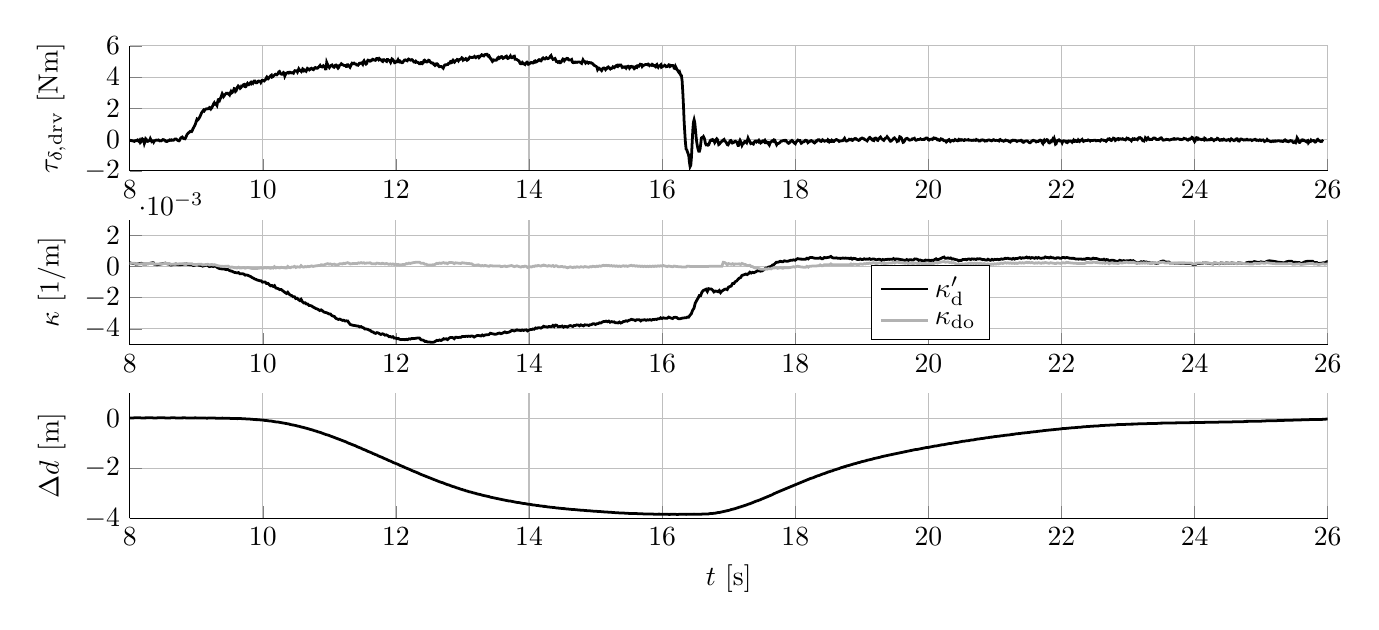
\begin{tikzpicture}

\begin{axis}[%
width=0.95092\figurewidth,
height=0.264706\figureheight,
at={(0\figurewidth,0\figureheight)},
scale only axis,
every outer x axis line/.append style={black},
every x tick label/.append style={font=\color{black}},
xmin=8,
xmax=26,
xlabel={$t$ [s]},
xlabel near ticks,
xmajorgrids,
every outer y axis line/.append style={black},
every y tick label/.append style={font=\color{black}},
ymin=-4,
ymax=1,
ylabel={$\Delta d$ [m]},
ylabel near ticks,
ymajorgrids,
axis x line*=bottom,
axis y line*=left
]
\addplot [color=black,solid,forget plot, line width=1.0]
  table[row sep=crcr]{%
7.97475	0.0192920030020045\\
7.99575	0.0102367716335747\\
8.01475	0.0110092538667868\\
8.03575	0.011781736100001\\
8.05475	0.0125501715600205\\
8.07575	0.0151647864525835\\
8.09475	0.0159329770925436\\
8.11575	0.01669703151512\\
8.13475	0.0174610859375766\\
8.15575	0.0182249062484012\\
8.17475	0.00915654519675346\\
8.19575	0.0117624464489969\\
8.21475	0.012521670864388\\
8.23575	0.0132769360025944\\
8.25475	0.0140322011406795\\
8.27575	0.0147867451413837\\
8.29475	0.0173832225006865\\
8.31575	0.0181337531261532\\
8.33475	0.0188832196892919\\
8.35575	0.00980052475061166\\
8.37475	0.0105459985186775\\
8.39575	0.0112901102613603\\
8.41475	0.0138758527014375\\
8.43575	0.0146158843271005\\
8.45475	0.0153541018621643\\
8.47575	0.0160882508131697\\
8.49475	0.0168223997639592\\
8.51575	0.0193997926535481\\
8.53475	0.0102993277161327\\
8.55575	0.0110271061548572\\
8.57375	0.0117520816171885\\
8.59575	0.0124729618927266\\
8.61475	0.0131938421681128\\
8.63575	0.0157565387842329\\
8.65475	0.0164699603677905\\
8.67675	0.0171833819509222\\
8.69475	0.00806444217416979\\
8.71575	0.00876981802949306\\
8.73475	0.0094751938846005\\
8.75575	0.012020635037103\\
8.77475	0.0127173572975749\\
8.79575	0.0134140795578039\\
8.81475	0.0141052538968958\\
8.83575	0.0147926992069012\\
8.85475	0.00565173100270755\\
8.87575	0.00817716069143071\\
8.89475	0.00885469501134528\\
8.91575	0.00953222933121145\\
8.93475	0.0102024196375838\\
8.95575	0.0108694020412856\\
8.97475	0.0133804537655133\\
8.99575	0.0140389928246996\\
9.01475	0.00486623155230204\\
9.03575	0.00552201727996504\\
9.05475	0.00616840049492673\\
9.07575	0.00865589500303621\\
9.09475	0.00929983792249578\\
9.11575	0.00993314004957613\\
9.13475	0.0105645944822528\\
9.15575	0.00136739935407659\\
9.17375	0.00383011706586966\\
9.19575	0.00444843927862326\\
9.21475	0.00506676149119922\\
9.23575	0.00567199934432505\\
9.25475	0.0062765485550873\\
9.27575	0.00872364729132125\\
9.29475	-0.000515037747212066\\
9.31575	7.51008405006637e-005\\
9.33475	0.000664518005116577\\
9.35575	0.00123961155809793\\
9.37475	0.00181470511131954\\
9.39575	0.00423014050066373\\
9.41475	-0.00503939526456687\\
9.43575	-0.00447997802309041\\
9.45475	-0.00392293966673307\\
9.47675	-0.00337982743659238\\
9.49475	-0.000995429495345146\\
9.51575	-0.0102848643832631\\
9.53475	-0.00975868412290559\\
9.55575	-0.00923250386043284\\
9.57475	-0.00871060503098464\\
9.59575	-0.00820198280384155\\
9.61475	-0.0175225274037616\\
9.63575	-0.0151789618361451\\
9.65475	-0.0146885240495598\\
9.67575	-0.0141980862597304\\
9.69475	-0.0235434009507118\\
9.71575	-0.0230717760581602\\
9.73475	-0.0226001511605602\\
9.75575	-0.0319653511451543\\
9.77375	-0.0296739289811105\\
9.79575	-0.0292217489946247\\
9.81475	-0.0386079725665911\\
9.83575	-0.0381758742489913\\
9.85475	-0.0475732646165619\\
9.87575	-0.047151279090647\\
9.89475	-0.056569480963645\\
9.91575	-0.0561581070252895\\
9.93475	-0.0655876800888771\\
9.95575	-0.0651976807178221\\
9.97475	-0.0746373469668731\\
9.99575	-0.0724225970444881\\
10.01475	-0.0818843890215435\\
10.03575	-0.0913461809906604\\
10.05475	-0.0909927048841155\\
10.07575	-0.100477292672049\\
10.09475	-0.109961880445796\\
10.11575	-0.109632565237939\\
10.13475	-0.119140627592706\\
10.15575	-0.128648689926209\\
10.17475	-0.1381743299189\\
10.19575	-0.147706554277979\\
10.21475	-0.147408725886988\\
10.23575	-0.156960123763747\\
10.25475	-0.166517206393632\\
10.27675	-0.176074288982596\\
10.29475	-0.185652315639278\\
10.31575	-0.195234961359317\\
10.33475	-0.20481760702509\\
10.35575	-0.2144230411913\\
10.37475	-0.224031962288131\\
10.39575	-0.233640883315251\\
10.41475	-0.253104996718574\\
10.43575	-0.262740911495657\\
10.45475	-0.272376826182709\\
10.47575	-0.282039554130982\\
10.49475	-0.291703185347273\\
10.51575	-0.311197973581052\\
10.53475	-0.320890047066243\\
10.55575	-0.330582120432267\\
10.57475	-0.350107003759502\\
10.59575	-0.361659788278184\\
10.61475	-0.371381029993247\\
10.63575	-0.390936143416423\\
10.65475	-0.400687276579357\\
10.67575	-0.420269376028087\\
10.69475	-0.430025205561287\\
10.71475	-0.449638038938924\\
10.73475	-0.459419778120489\\
10.75575	-0.479039176212142\\
10.77475	-0.500512935507703\\
10.79575	-0.510325982400716\\
10.81475	-0.529978044168297\\
10.83575	-0.549654439173525\\
10.85475	-0.559499476242842\\
10.87575	-0.579185656528794\\
10.89475	-0.600722876367171\\
10.91575	-0.620432055059132\\
10.93475	-0.640152470662356\\
10.95575	-0.659895064270446\\
10.97475	-0.669806025462607\\
10.99575	-0.689561958408783\\
11.01475	-0.711165100630625\\
11.03575	-0.730941704673773\\
11.05475	-0.750733172437128\\
11.07675	-0.770544345480322\\
11.09475	-0.79218128524242\\
11.11575	-0.812008866823357\\
11.13475	-0.831855123353148\\
11.15575	-0.851701379367192\\
11.17475	-0.871566396030516\\
11.19575	-0.893272395489316\\
11.21475	-0.913154201904336\\
11.23575	-0.933056342833352\\
11.25475	-0.952974114182806\\
11.27575	-0.984547632700013\\
11.29475	-1.00448745725449\\
11.31575	-1.02444154891247\\
11.33475	-1.0462182208303\\
11.35475	-1.06619592189789\\
11.37475	-1.08618662730424\\
11.39575	-1.10617733193876\\
11.41475	-1.13784775437816\\
11.43575	-1.15787530092756\\
11.45475	-1.17790284663518\\
11.47575	-1.19795801176336\\
11.49475	-1.2296756398578\\
11.51575	-1.24974018539452\\
11.53475	-1.26983396288923\\
11.55575	-1.29175488931589\\
11.57475	-1.32168963983831\\
11.59575	-1.34182206582847\\
11.61475	-1.36196080712434\\
11.63575	-1.38391801145529\\
11.65475	-1.41392231048168\\
11.67575	-1.43409810331625\\
11.69475	-1.45609153298669\\
11.71575	-1.47630088689379\\
11.73475	-1.50634717758935\\
11.75575	-1.52837670744671\\
11.77475	-1.54862432872019\\
11.79575	-1.56887376685756\\
11.81475	-1.59895745266051\\
11.83575	-1.62105852151793\\
11.85475	-1.64134440618276\\
11.87675	-1.67146618309826\\
11.89475	-1.69360254590208\\
11.91575	-1.71392452943821\\
11.93475	-1.73424984078035\\
11.95475	-1.76625525867257\\
11.97475	-1.78661292199255\\
11.99575	-1.80697532772751\\
12.01475	-1.82736818211669\\
12.03575	-1.84957383300225\\
12.05475	-1.87980710507533\\
12.07575	-1.90023458904491\\
12.09475	-1.92247409725301\\
12.11575	-1.94290884222469\\
12.13475	-1.97320492351693\\
12.15575	-1.9936664059275\\
12.17475	-2.01594764898375\\
12.19575	-2.03644243433667\\
12.21475	-2.05693721840334\\
12.23575	-2.08727710876642\\
12.25475	-2.10961423002262\\
12.27575	-2.13014155102055\\
12.29475	-2.15068016230599\\
12.31575	-2.17304828307835\\
12.33475	-2.19360731072144\\
12.35575	-2.2240135836519\\
12.37475	-2.24460342408276\\
12.39575	-2.26700166805599\\
12.41475	-2.28760448660658\\
12.43575	-2.30822417951819\\
12.45475	-2.32884387123218\\
12.47575	-2.35128491191237\\
12.49475	-2.37193343526057\\
12.51575	-2.39258195745427\\
12.53475	-2.41324523091628\\
12.55475	-2.43572797727108\\
12.57475	-2.45640424539533\\
12.59575	-2.47709564631878\\
12.61475	-2.49779851398592\\
12.63575	-2.52030726455211\\
12.65475	-2.54102552138361\\
12.67675	-2.56175377648349\\
12.69475	-2.57264633907058\\
12.71575	-2.59339054826137\\
12.73475	-2.61594769527943\\
12.75575	-2.63670006151126\\
12.77475	-2.65746834493582\\
12.79575	-2.66840760041216\\
12.81475	-2.69098701046027\\
12.83575	-2.71177779189219\\
12.85475	-2.73257429607969\\
12.87575	-2.7435348286929\\
12.89475	-2.76434699986978\\
12.91575	-2.78516339455605\\
12.93475	-2.79794708821252\\
12.95575	-2.8187785416546\\
12.97475	-2.83961328095823\\
12.99575	-2.85061189249117\\
13.01475	-2.87146128972502\\
13.03575	-2.8824765582225\\
13.05475	-2.90513059133957\\
13.07575	-2.91615946939531\\
13.09475	-2.93702596191593\\
13.11575	-2.94805619703663\\
13.13475	-2.95909911763904\\
13.15575	-2.97997886414001\\
13.17475	-2.99102244337412\\
13.19575	-3.00207723180894\\
13.21775	-3.02477006214636\\
13.23675	-3.03582524638322\\
13.25775	-3.04688945853148\\
13.27775	-3.057953670488\\
13.29775	-3.07885497400228\\
13.31775	-3.08992659667009\\
13.33775	-3.10099821920998\\
13.35775	-3.1120705934499\\
13.37775	-3.1231475276514\\
13.39775	-3.13422446177905\\
13.41775	-3.15513844893325\\
13.43775	-3.16621850913712\\
13.45775	-3.17729856930805\\
13.47875	-3.18837883547162\\
13.49775	-3.19945974990672\\
13.51775	-3.21054066433434\\
13.53775	-3.22162114442986\\
13.55775	-3.23270055588459\\
13.57775	-3.24377996733927\\
13.59775	-3.25485805002761\\
13.61775	-3.26593351668579\\
13.63775	-3.27700898333019\\
13.65775	-3.28808196061831\\
13.67775	-3.2991509571586\\
13.69775	-3.31021995364729\\
13.71775	-3.31144864369203\\
13.73775	-3.32250856309354\\
13.75775	-3.33356848237861\\
13.77775	-3.34462279538858\\
13.79775	-3.35567095174258\\
13.81775	-3.36671910788491\\
13.83675	-3.36792337319047\\
13.85775	-3.37895700585227\\
13.87775	-3.38999063817455\\
13.89775	-3.40101440245903\\
13.91775	-3.41203068196234\\
13.93775	-3.41321076126536\\
13.95775	-3.42421463657679\\
13.97775	-3.43521067238948\\
13.99775	-3.43637059089851\\
14.01775	-3.44554787674929\\
14.03775	-3.45652072608961\\
14.05775	-3.46749357447888\\
14.07775	-3.46861146856658\\
14.09775	-3.47955814584902\\
14.11775	-3.49050482189371\\
14.13775	-3.49159317636916\\
14.15775	-3.50251066310815\\
14.17775	-3.51342814827903\\
14.19775	-3.51448367009365\\
14.21775	-3.52536892568772\\
14.23775	-3.52461303644915\\
14.25775	-3.53546728853175\\
14.27875	-3.54631726199691\\
14.29775	-3.54733171669943\\
14.31775	-3.5581463052772\\
14.33775	-3.55912258970296\\
14.35775	-3.56993422999991\\
14.37775	-3.5708706614157\\
14.39775	-3.58164094302521\\
14.41775	-3.59060162693585\\
14.43775	-3.59149254652912\\
14.45575	-3.60221846802519\\
14.47775	-3.60310582333846\\
14.49775	-3.61378443907823\\
14.51775	-3.61462823953736\\
14.53775	-3.6154662260371\\
14.55775	-3.62609464552377\\
14.57775	-3.62688845608264\\
14.59775	-3.63569593952689\\
14.61775	-3.63643696892169\\
14.63775	-3.64701237783605\\
14.65775	-3.64774093988069\\
14.67775	-3.64842647809312\\
14.69775	-3.65894616514372\\
14.71775	-3.65961627518546\\
14.73775	-3.67007763634757\\
14.75775	-3.67070507631799\\
14.77775	-3.67933128159756\\
14.79775	-3.67989815460883\\
14.81775	-3.6804650199155\\
14.83775	-3.69084200855945\\
14.85775	-3.69134595433466\\
14.87775	-3.70168329306161\\
14.89775	-3.70216018846987\\
14.91775	-3.70259899373611\\
14.93775	-3.71287092045493\\
14.95775	-3.71327905635374\\
14.97775	-3.721662784228\\
14.99775	-3.72203437718347\\
15.01775	-3.72237004744895\\
15.03775	-3.73250511202743\\
15.05675	-3.7328076033019\\
15.07775	-3.73307035928338\\
15.09775	-3.74313430469604\\
15.11775	-3.74154209976253\\
15.13775	-3.75156052734598\\
15.15775	-3.75171984617338\\
15.17775	-3.75187915355393\\
15.19775	-3.76182104099342\\
15.21775	-3.76190666733022\\
15.23775	-3.76199228172278\\
15.25775	-3.77185632812749\\
15.27775	-3.77003830400559\\
15.29775	-3.77988044903719\\
15.31775	-3.77983255408491\\
15.33775	-3.77976765253154\\
15.35775	-3.78953376707377\\
15.37775	-3.78940648422835\\
15.39775	-3.78926520146602\\
15.41775	-3.78729165042651\\
15.43775	-3.7969134441494\\
15.45775	-3.79669535125638\\
15.47775	-3.79647724509456\\
15.49775	-3.80601856291809\\
15.51775	-3.80572347782249\\
15.53775	-3.80542837931904\\
15.55775	-3.81305182454668\\
15.57775	-3.81267981613263\\
15.59775	-3.81230603249014\\
15.61775	-3.81185743873874\\
15.63775	-3.82123825075958\\
15.65775	-3.82078473936559\\
15.67775	-3.81841925810586\\
15.69775	-3.81789463333032\\
15.71775	-3.82718946238905\\
15.73775	-3.82658967192133\\
15.75775	-3.82598986841646\\
15.77775	-3.82537781192191\\
15.79775	-3.83268818301353\\
15.81575	-3.83201429492203\\
15.83775	-3.83132374051984\\
15.85775	-3.83057712765288\\
15.87875	-3.83965866622396\\
15.89775	-3.83889280569347\\
15.91775	-3.83622759326126\\
15.93775	-3.83540982609757\\
15.95775	-3.83456920034985\\
15.97775	-3.84350971045399\\
15.99775	-3.8426226388061\\
16.01775	-3.84171062353926\\
16.03775	-3.83890580419231\\
16.05775	-3.83795149923933\\
16.07775	-3.83696924852713\\
16.09775	-3.84577702859179\\
16.11775	-3.84475778735532\\
16.13775	-3.84370911681103\\
16.15775	-3.84077407320375\\
16.17775	-3.83969240698468\\
16.19775	-3.8385790535428\\
16.21775	-3.84726417922459\\
16.23775	-3.84612280257511\\
16.25775	-3.84309294743081\\
16.27775	-3.84189477107503\\
16.29775	-3.84069658694136\\
16.31775	-3.83946451090009\\
16.33775	-3.83821260300857\\
16.35775	-3.84492950088756\\
16.37775	-3.8436425367991\\
16.39775	-3.84234013054357\\
16.41575	-3.84103771806388\\
16.43775	-3.83970087538102\\
16.45775	-3.83835134284908\\
16.47775	-3.83514239972558\\
16.49775	-3.84358383571237\\
16.51775	-3.8421906679053\\
16.53775	-3.84079749537922\\
16.55775	-3.83937107929864\\
16.57775	-3.83793786617861\\
16.59775	-3.83464336412208\\
16.61775	-3.83317781029019\\
16.63775	-3.83170821955744\\
16.65775	-3.83023862548866\\
16.67875	-3.82873882269165\\
16.69775	-3.8253737438368\\
16.71775	-3.81404653747192\\
16.73775	-3.81251599197631\\
16.75775	-3.81098485732628\\
16.77775	-3.79776454629563\\
16.79775	-3.79620829982363\\
16.81775	-3.78482732154849\\
16.83775	-3.77158050326777\\
16.85775	-3.77000291797565\\
16.87775	-3.75860069226795\\
16.89775	-3.74533158593049\\
16.91775	-3.73391185131421\\
16.93775	-3.72249211584875\\
16.95775	-3.70920497047884\\
16.97775	-3.69777142381375\\
16.99775	-3.68633787659968\\
17.01775	-3.67303679936506\\
17.03775	-3.65176861972032\\
17.05775	-3.64032490128204\\
17.07775	-3.62701395554731\\
17.09775	-3.61556363199889\\
17.11775	-3.59242326212443\\
17.13775	-3.5809719738683\\
17.15775	-3.55782841695654\\
17.17775	-3.5463749633614\\
17.19775	-3.52509717273239\\
17.21775	-3.51177828104654\\
17.23775	-3.49050064663124\\
17.25575	-3.47718318156569\\
17.27775	-3.45590902309483\\
17.29775	-3.43276926523617\\
17.31775	-3.42132248718651\\
17.33775	-3.39818946091461\\
17.35775	-3.37692188483834\\
17.37775	-3.35379365724051\\
17.39775	-3.33253562962848\\
17.41775	-3.30941236795084\\
17.43775	-3.29798551496037\\
17.45775	-3.27487489836936\\
17.47875	-3.2536292353222\\
17.49775	-3.23052755066455\\
17.51775	-3.20929691131087\\
17.53775	-3.18620165814609\\
17.55775	-3.16498200179861\\
17.57775	-3.14190466277779\\
17.59775	-3.12069153979614\\
17.61775	-3.09762773242324\\
17.63775	-3.07643444846966\\
17.65775	-3.05337739672582\\
17.67775	-3.02051167254572\\
17.69775	-2.99934037118058\\
17.71575	-2.97630579991426\\
17.73475	-2.95515282302964\\
17.75575	-2.93214273979585\\
17.77475	-2.91099538214878\\
17.79575	-2.88800639945098\\
17.81475	-2.8668847643898\\
17.83475	-2.84390098439726\\
17.85475	-2.82094111419403\\
17.87575	-2.7998467908183\\
17.89475	-2.77689094117645\\
17.91575	-2.75582268438932\\
17.93475	-2.73289620057995\\
17.95575	-2.71183058985353\\
17.97475	-2.68893292268848\\
17.99575	-2.66603704506092\\
18.01475	-2.64500136233796\\
18.03575	-2.62213699438963\\
18.05475	-2.6011322676487\\
18.07575	-2.57826964389823\\
18.09475	-2.55729671337684\\
18.11575	-2.53446500664695\\
18.13475	-2.51163671879857\\
18.15575	-2.49069623886722\\
18.17475	-2.46789771795305\\
18.19575	-2.44696177398298\\
18.21475	-2.4241969266921\\
18.23575	-2.4032893710139\\
18.25475	-2.39035708449371\\
18.27675	-2.36948275608285\\
18.29475	-2.34675188554879\\
18.31575	-2.3258852183122\\
18.33475	-2.30318846183999\\
18.35575	-2.29217378281914\\
18.37475	-2.26948666247428\\
18.39575	-2.24867901832617\\
18.41475	-2.22601634309247\\
18.43575	-2.21504594116981\\
18.45475	-2.19241716802745\\
18.47575	-2.17164267165506\\
18.49375	-2.14902641383749\\
18.51575	-2.13811147096564\\
18.53475	-2.11551627306384\\
18.55575	-2.10461500969842\\
18.57475	-2.08205293797691\\
18.59575	-2.06134366523063\\
18.61475	-2.04862379252334\\
18.63575	-2.02794635775732\\
18.65475	-2.01524383623103\\
18.67575	-1.99458258019731\\
18.69475	-1.97208495801481\\
18.71575	-1.96126583365789\\
18.73475	-1.93878582448903\\
18.75575	-1.92799728241791\\
18.77475	-1.9055308001459\\
18.79575	-1.89476063082139\\
18.81475	-1.88215185555593\\
18.83575	-1.86156570639638\\
18.85475	-1.84897661689003\\
18.87575	-1.8284192678435\\
18.89475	-1.81768942387379\\
18.91575	-1.80513045378019\\
18.93475	-1.7846010155803\\
18.95575	-1.77205047619208\\
18.97475	-1.76136934909578\\
18.99575	-1.7390187980904\\
19.01475	-1.72834409984552\\
19.03575	-1.715842940268\\
19.05475	-1.7051944363935\\
19.07675	-1.68287055807586\\
19.09475	-1.67224398780801\\
19.11575	-1.66162076027156\\
19.13475	-1.64915058001333\\
19.15575	-1.63854961236897\\
19.17475	-1.61627629745785\\
19.19475	-1.6056774457141\\
19.21475	-1.59510102723604\\
19.23575	-1.58267980974462\\
19.25475	-1.57210446131091\\
19.27575	-1.55970642593204\\
19.29475	-1.53932549502146\\
19.31575	-1.52877371917271\\
19.33475	-1.51639806779084\\
19.35575	-1.50586728191789\\
19.37475	-1.4934939373553\\
19.39575	-1.48298430940869\\
19.41475	-1.47063029248028\\
19.43575	-1.46012383058725\\
19.45475	-1.44963469141359\\
19.47575	-1.4373016256558\\
19.49475	-1.42681646431929\\
19.51575	-1.41450373381811\\
19.53475	-1.40403448036814\\
19.55575	-1.39356997932516\\
19.57475	-1.38127703851148\\
19.59575	-1.37082713804182\\
19.61475	-1.36038273662561\\
19.63575	-1.34810911351406\\
19.65475	-1.33767810444908\\
19.67575	-1.32541112656272\\
19.69475	-1.31499861941353\\
19.71575	-1.30458611197811\\
19.73475	-1.29233876662496\\
19.75575	-1.28194444189665\\
19.77475	-1.26970833038862\\
19.79475	-1.25932207956579\\
19.81475	-1.24894568650874\\
19.83575	-1.2465569150153\\
19.85475	-1.23618939588184\\
19.87675	-1.22398976787856\\
19.89475	-1.21363112096305\\
19.91575	-1.20328208904344\\
19.93475	-1.1911004810337\\
19.95575	-1.18075945642613\\
19.97475	-1.16858862192142\\
19.99575	-1.16809437885049\\
20.01475	-1.15777090823069\\
20.03575	-1.14561888552947\\
20.05475	-1.13531295033739\\
20.07575	-1.12500701492711\\
20.09475	-1.11287373895195\\
20.11575	-1.11241473792047\\
20.13475	-1.1002869656216\\
20.15575	-1.0900119576574\\
20.17475	-1.07974119652393\\
20.19575	-1.06763143724726\\
20.21475	-1.05737491278425\\
20.23575	-1.05695137257807\\
20.25475	-1.0448597089454\\
20.27575	-1.03462184284555\\
20.29475	-1.02254837153641\\
20.31575	-1.01231309706033\\
20.33475	-1.01192359522418\\
20.35575	-0.99986841513772\\
20.37375	-0.989651028185958\\
20.39575	-0.979450713163986\\
20.41475	-0.967413914049937\\
20.43575	-0.967044253483559\\
20.45475	-0.956862875764455\\
20.47575	-0.944844525546448\\
20.49475	-0.934663971859989\\
20.51575	-0.922664104482245\\
20.53475	-0.922330712855465\\
20.55575	-0.91216913351362\\
20.57475	-0.900187736687549\\
20.59575	-0.899872484106123\\
20.61475	-0.88972985806425\\
20.63575	-0.877766862341288\\
20.65475	-0.867639625153167\\
20.67675	-0.867345920149545\\
20.69475	-0.855401187294713\\
20.71575	-0.845291809890534\\
20.73475	-0.835186673141679\\
20.75575	-0.833090190479965\\
20.77475	-0.822998459944029\\
20.79575	-0.812911762838456\\
20.81475	-0.810833091683942\\
20.83575	-0.800758708067888\\
20.85475	-0.790690088457324\\
20.87575	-0.778798473480899\\
20.89475	-0.778571391100708\\
20.91575	-0.768520374446958\\
20.93475	-0.756645584691825\\
20.95575	-0.756435025460469\\
20.97475	-0.74640101644916\\
20.99575	-0.734542431423252\\
21.01475	-0.734347785974244\\
21.03575	-0.724330061702111\\
21.05475	-0.722317493834273\\
21.07475	-0.712307489421444\\
21.09475	-0.702305194717727\\
21.11575	-0.700307299004594\\
21.13475	-0.690311584099221\\
21.15575	-0.680323729064325\\
21.17475	-0.67833952510015\\
21.19575	-0.668357144874531\\
21.21475	-0.668213321511185\\
21.23575	-0.658243203899167\\
21.25475	-0.646440873730418\\
21.27575	-0.646309153483653\\
21.29475	-0.636350111564835\\
21.31575	-0.624559107093531\\
21.33475	-0.62443809781025\\
21.35575	-0.614488834546192\\
21.37475	-0.612538634208077\\
21.39575	-0.602596016772015\\
21.41475	-0.592655131200852\\
21.43575	-0.592545085579905\\
21.45475	-0.580778449585112\\
21.47675	-0.580675314134878\\
21.49475	-0.570741309746913\\
21.51575	-0.568811532552916\\
21.53475	-0.558882827858227\\
21.55575	-0.548954123150139\\
21.57475	-0.547028485040855\\
21.59575	-0.537103425648608\\
21.61475	-0.537009272777278\\
21.63575	-0.527086096152945\\
21.65475	-0.525162731270038\\
21.67475	-0.515239607873368\\
21.69475	-0.515147569227548\\
21.71575	-0.503393467255724\\
21.73475	-0.493470392938101\\
21.75575	-0.493376734162036\\
21.77475	-0.481620982427601\\
21.79575	-0.481526884276721\\
21.81475	-0.471598903589263\\
21.83575	-0.471501817145121\\
21.85475	-0.459741644099296\\
21.87575	-0.459639325779067\\
21.89475	-0.449706135114753\\
21.91575	-0.447770810957783\\
21.93475	-0.437830633909568\\
21.95575	-0.437721299811368\\
21.97475	-0.427778851879604\\
21.99575	-0.425829021851848\\
22.01475	-0.41588011918138\\
22.03575	-0.415758749345038\\
22.05475	-0.413798229842849\\
22.07575	-0.403838916458506\\
22.09475	-0.403705933071029\\
22.11575	-0.393734594749767\\
22.13475	-0.391761728252909\\
22.15575	-0.381784717225416\\
22.17475	-0.381630481532898\\
22.19575	-0.379643699877434\\
22.21475	-0.369651728705335\\
22.23575	-0.369482452817778\\
22.25475	-0.359482585026059\\
22.27675	-0.357471843653695\\
22.29475	-0.35728621363182\\
22.31475	-0.347270060239794\\
22.33475	-0.345241029634614\\
22.35575	-0.34503786143082\\
22.37475	-0.33500424336885\\
22.39575	-0.332955674732693\\
22.41475	-0.332733925941548\\
22.43575	-0.322681805192136\\
22.45475	-0.322447125332984\\
22.47575	-0.320371404222663\\
22.49475	-0.310299893783001\\
22.51575	-0.310044167319107\\
22.53475	-0.3079477899286\\
22.55575	-0.307686367491885\\
22.57475	-0.297578707858773\\
22.59575	-0.295461097238006\\
22.61475	-0.295178908300119\\
22.63575	-0.294879154136237\\
22.65475	-0.284745776381794\\
22.67575	-0.28260653077026\\
22.69475	-0.282284282231744\\
22.71575	-0.281959555640646\\
22.73475	-0.26996851137618\\
22.75575	-0.269623689142573\\
22.77475	-0.269277539201426\\
22.79575	-0.268931389186354\\
22.81475	-0.266727165937027\\
22.83575	-0.256529959844138\\
22.85475	-0.256161933963092\\
22.87575	-0.255773489467752\\
22.89475	-0.253547235090579\\
22.91575	-0.253157029119124\\
22.93475	-0.252748046359764\\
22.95575	-0.25050079214558\\
22.97475	-0.240259440545129\\
22.99575	-0.239830535641102\\
23.01475	-0.239401630677913\\
23.03575	-0.23713021623724\\
23.05475	-0.236682150484727\\
23.07675	-0.236234084677501\\
23.09475	-0.23578175413768\\
23.11575	-0.235315421801633\\
23.13475	-0.233009529175335\\
23.15575	-0.222708893771217\\
23.17475	-0.222225308642146\\
23.19575	-0.221741723470785\\
23.21475	-0.219412615948401\\
23.23575	-0.218912897115363\\
23.25475	-0.218413178245576\\
23.27575	-0.217907770919627\\
23.29475	-0.215552482060274\\
23.31575	-0.215037839095183\\
23.33475	-0.214517204805209\\
23.35575	-0.213988922817284\\
23.37475	-0.21346064080301\\
23.39575	-0.211085291379539\\
23.41475	-0.210544715349286\\
23.43575	-0.210004139297642\\
23.45475	-0.199628764262677\\
23.47575	-0.197235809817357\\
23.49475	-0.196684329125797\\
23.51575	-0.196127280736329\\
23.53475	-0.195566314020142\\
23.55575	-0.195005347291583\\
23.57475	-0.194439367086998\\
23.59575	-0.192028479632683\\
23.61475	-0.191459460080754\\
23.63575	-0.19088593477021\\
23.65475	-0.190310295746342\\
23.67575	-0.189734656716263\\
23.69475	-0.187313158929246\\
23.71575	-0.186732319374808\\
23.73475	-0.186151479816549\\
23.75575	-0.185567689638091\\
23.77475	-0.184983039984531\\
23.79575	-0.182556171172514\\
23.81475	-0.181969472473277\\
23.83575	-0.181382361578041\\
23.85475	-0.180795250681765\\
23.87675	-0.180207127945918\\
23.89475	-0.177776550886968\\
23.91575	-0.177188274484795\\
23.93475	-0.176600060165991\\
23.95575	-0.176011850789984\\
23.97475	-0.175423641413779\\
23.99575	-0.172994341649802\\
24.01475	-0.172407360246843\\
24.03575	-0.17182042502172\\
24.05475	-0.171235754492189\\
24.07575	-0.168808864337037\\
24.09475	-0.168224452342419\\
24.11575	-0.167643092932245\\
24.13475	-0.167061733521392\\
24.15575	-0.166480854637668\\
24.17475	-0.164061671024415\\
24.19575	-0.163484537657905\\
24.21475	-0.162908272655797\\
24.23575	-0.162336193704771\\
24.25475	-0.161764114751796\\
24.27575	-0.159351431706475\\
24.29475	-0.158785149071815\\
24.31575	-0.15821886643393\\
24.33475	-0.157654297367542\\
24.35575	-0.157094468285609\\
24.37475	-0.154692977819555\\
24.39475	-0.154135423729705\\
24.41475	-0.153582624487941\\
24.43575	-0.153029825241883\\
24.45475	-0.152479731174282\\
24.47575	-0.150093127965597\\
24.49475	-0.149547858931138\\
24.51575	-0.149005912139142\\
24.53475	-0.148468603639335\\
24.55575	-0.14793129513443\\
24.57475	-0.145556790567061\\
24.59575	-0.145027809641686\\
24.61475	-0.144498828710309\\
24.63575	-0.143974262711656\\
24.65475	-0.14161314657792\\
24.67675	-0.141092804442537\\
24.69475	-0.140577528806424\\
24.71575	-0.140066088468443\\
24.73475	-0.139554648123989\\
24.75575	-0.127379163739635\\
24.77475	-0.126876847782723\\
24.79575	-0.126374531819728\\
24.81475	-0.12587835107104\\
24.83575	-0.123545190113769\\
24.85475	-0.123052188727743\\
24.87575	-0.122565982262649\\
24.89475	-0.12208246086227\\
24.91575	-0.121598939455362\\
24.93475	-0.119282931741763\\
24.95575	-0.118809038141957\\
24.97475	-0.118335144535699\\
24.99475	-0.117869165387841\\
25.01475	-0.115565526134096\\
25.03575	-0.115101397585827\\
25.05475	-0.114645866400604\\
25.07575	-0.104362240337098\\
25.09475	-0.102068721635857\\
25.11575	-0.101623745875707\\
25.13475	-0.101179547836467\\
25.15575	-0.100735349791173\\
25.17475	-0.0984620639039369\\
25.19575	-0.0980280383907952\\
25.21475	-0.0975941801297071\\
25.23575	-0.0971704769741129\\
25.25475	-0.0949081716010047\\
25.27575	-0.0944852474629143\\
25.29475	-0.0940720287614116\\
25.31575	-0.0936588100537299\\
25.33475	-0.091408636215109\\
25.35575	-0.0811764649502562\\
25.37475	-0.080773906540113\\
25.39575	-0.0803731257249156\\
25.41475	-0.0781435345592447\\
25.43575	-0.0777518265430044\\
25.45475	-0.0773625716901654\\
25.47675	-0.0769819174987796\\
25.49475	-0.0747636285702553\\
25.51575	-0.074386129810577\\
25.53475	-0.0740167438029373\\
25.55575	-0.0736473577896954\\
25.57475	-0.0714444754385148\\
25.59475	-0.0710865794453386\\
25.61475	-0.0608988829346249\\
25.63575	-0.0605453162097178\\
25.65475	-0.0583622748727342\\
25.67575	-0.0580160935084244\\
25.69475	-0.057675016920276\\
25.71575	-0.057340771961909\\
25.73475	-0.0551699352850195\\
25.75575	-0.054841591828851\\
25.77475	-0.0545194956790169\\
25.79575	-0.0541973995243406\\
25.81475	-0.0520456985259936\\
25.83575	-0.0517359468659291\\
25.85475	-0.0514261952008899\\
25.87575	-0.0511236962827208\\
25.89475	-0.0489907001495524\\
25.91575	-0.0486934639604302\\
25.93475	-0.0385741872183556\\
25.95575	-0.0382896041998011\\
25.97475	-0.0361695456074171\\
25.99575	-0.035893778524128\\
26.01475	-0.0356219441974561\\
26.03575	-0.0353501098673292\\
26.05475	-0.0350875782305722\\
26.07575	-0.0329936357873439\\
26.09475	-0.0327345948465121\\
26.11575	-0.0324855883148762\\
26.13475	-0.0322393259051221\\
26.15575	-0.0301584491871236\\
26.17475	-0.0299228935741684\\
26.19575	-0.0296893265268885\\
26.21475	-0.0294557594767038\\
26.23575	-0.0292332111252684\\
26.25375	-0.0271781324105707\\
26.27675	-0.026957100918338\\
26.29475	-0.0267475874699166\\
26.31575	-0.0265388470853414\\
26.33475	-0.0244963357240136\\
26.35575	-0.0242994924624216\\
26.37475	-0.0241027064278638\\
26.39575	-0.023906275694304\\
26.41475	-0.0237210081769756\\
26.43575	-0.0217024972568796\\
26.45475	-0.0215182063025181\\
26.47575	-0.0213439168330472\\
26.49475	-0.0211696273619051\\
26.51575	-0.0191638602105644\\
26.53475	-0.0189998992248821\\
26.55575	-0.01883593823759\\
26.57475	-0.0186737250654296\\
26.59575	-0.0185193305788252\\
26.61475	-0.0165323865976417\\
26.63575	-0.016380084635558\\
26.65475	-0.0162343795637829\\
26.67575	-0.0160886744912112\\
26.69475	-0.0141129155610868\\
26.71575	-0.0139749058240453\\
26.73475	-0.0138368960862145\\
26.75575	-0.0137010890435283\\
26.77475	-0.0135696631388984\\
26.79575	-0.0116062039917422\\
26.81475	-0.0114768812570367\\
26.83575	-0.0113508113734127\\
26.85475	-0.0112247414893365\\
26.87575	-0.011100391064117\\
26.89475	-0.00914651306804437\\
26.91575	-0.00902445769650351\\
26.93375	-0.00890364923307541\\
26.95575	-0.00878415727779736\\
26.97475	-0.00866466532257082\\
26.99575	-0.00671395738813896\\
27.01475	-0.00659547367930013\\
27.03575	-0.00647698997030899\\
27.05475	-0.00635813262282392\\
27.07675	-0.00623900490450024\\
27.09475	-0.00428812036512349\\
27.11575	-0.00416747031114451\\
27.13475	-0.00404595757205639\\
27.15575	-0.00392444483307264\\
27.17475	-0.0136308725962939\\
27.19575	-0.0116732499512464\\
27.21475	-0.0115475322477678\\
27.23575	-0.0114173288891024\\
27.25475	-0.0112855184665439\\
27.27575	-0.00932166615900565\\
27.29475	-0.0091834724068649\\
27.31575	-0.00904362604324982\\
27.33475	-0.00890377967917466\\
27.35575	-0.00875561566849914\\
27.37475	-0.0067733001321737\\
27.39575	-0.00662343234494411\\
27.41475	-0.00646287613500895\\
27.43575	-0.00630097322129153\\
27.45475	-0.00613907030702565\\
27.47575	-0.00413114299021\\
27.49475	-0.00395517761857445\\
27.51575	-0.00377921224658229\\
27.53475	-0.00358745052075848\\
27.55475	-0.00156200098774661\\
27.57475	-0.0111996445006035\\
27.59575	-0.0109894938979069\\
27.61475	-0.0107793432931516\\
27.63575	-0.0105675907255405\\
27.65475	-0.00850311326729081\\
27.67575	-0.00827288962851336\\
27.69475	-0.00803963161471088\\
27.71575	-0.00778740744225992\\
27.73475	-0.00753518326738645\\
27.75575	-0.00544353262227615\\
27.77475	-0.00516744490390364\\
27.79575	-0.00489135718316547\\
27.81475	-0.00460932780723589\\
27.83575	-0.00430759400181113\\
27.85475	-0.0120000354834313\\
27.87675	-0.0116902661845812\\
27.89475	-0.0113612001229404\\
27.91575	-0.0110321340556627\\
27.93475	-0.0106935394477032\\
27.95575	-0.00849844203363004\\
27.97475	-0.00814046958350367\\
27.99575	-0.00777072769358345\\
28.01475	-0.00738240205556906\\
28.03575	-0.00699407641251115\\
28.05475	-0.0047538282154429\\
28.07575	-0.00433384400583803\\
28.09475	-0.00391385979219949\\
28.11575	-0.0034780776581731\\
28.13475	-0.012854685563171\\
28.15575	-0.0105626358456261\\
28.17375	-0.0100914637328731\\
28.19575	-0.00960487529622478\\
28.21475	-0.00911828685145144\\
28.23575	-0.00677085326554305\\
28.25475	-0.00624966040978858\\
28.27575	-0.00572846754770406\\
28.29475	-0.00518481211157473\\
28.31575	-0.00462838807665644\\
28.33475	-0.00223037917727842\\
28.35575	-0.0114779556917979\\
28.37475	-0.0108858622144403\\
28.39575	-0.010293768726497\\
28.41475	-0.00967525810180536\\
28.43575	-0.00720405580481476\\
28.45475	-0.00657604701188808\\
28.47575	-0.00591949318426277\\
28.49475	-0.00525551761102205\\
28.51575	-0.00459154203101031\\
28.53475	-0.00205305123295174\\
28.55575	-0.00135325156269639\\
28.57475	-0.0104818132887061\\
28.59575	-0.00975037085818675\\
28.61475	-0.00901508191360145\\
28.63575	-0.00643418871762425\\
28.65475	-0.00566569111136772\\
28.67675	-0.00489543544236293\\
28.69475	-0.00412517976691706\\
28.71575	-0.00332116299223806\\
28.73475	-0.00251664451238698\\
28.75475	0.000136484806539716\\
28.77475	-0.00885338944448222\\
28.79575	-0.00801548533765972\\
28.81475	-0.00717488617831075\\
28.83575	-0.00630463682857396\\
28.85475	-0.00358575065616229\\
28.87575	-0.00271109544157033\\
28.89475	-0.00180969245277485\\
28.91575	-0.000908289459435885\\
28.93475	-1.6059165077742e-006\\
28.95575	-0.00889776245009344\\
28.97475	-0.00611652818384778\\
28.99575	-0.0051785088752907\\
29.01475	-0.00421890903573585\\
29.03575	-0.00325930919096873\\
29.05475	-0.00229233489995151\\
29.07575	0.000545326445211547\\
29.09475	0.0015317408794413\\
29.11575	0.00252653923127033\\
29.13475	-0.00628892180656448\\
29.15575	-0.00527733902293548\\
29.17475	-0.00240466957338903\\
29.19575	-0.00136963406813173\\
29.21475	-0.000334598560136179\\
29.23575	0.000709785663090656\\
29.25475	0.00176650827383895\\
29.27575	-0.00515079518277606\\
29.29475	-0.00408425835647908\\
29.31575	-0.00300764493143069\\
29.33475	-0.00193103150404639\\
29.35475	-0.000844851800253732\\
29.37475	0.00210352403499536\\
29.39575	0.00319822009990833\\
29.41475	0.00430247520595595\\
29.43575	-0.00441317035962774\\
29.45475	-0.00330219316658953\\
29.47675	-0.00218212170690446\\
29.49475	0.000797731600945983\\
29.51575	0.00192321346733548\\
29.53475	0.00305744466191005\\
29.55575	0.00419569777232232\\
29.57475	-0.00449255624223044\\
29.59575	-0.00149134989681787\\
29.61475	-0.000341998680694289\\
29.63575	0.000807352535920902\\
29.65475	0.00196414361750064\\
29.67575	0.00312299613955513\\
29.69475	0.00428184866181613\\
29.71575	-0.00252383855781613\\
29.73475	-0.00135699088359909\\
29.75575	-0.000190143209011229\\
29.77475	0.000982511794403784\\
29.79575	0.00215595128215007\\
29.81475	0.00332939077009931\\
29.83575	0.00636325720000519\\
29.85475	-0.00228433773495595\\
29.87575	-0.00110559726923798\\
29.89475	7.71865496793644e-005\\
29.91575	0.00126005733060275\\
29.93475	0.0024429730641593\\
29.95575	0.00548465971209922\\
29.97475	-0.00315568853792225\\
};
\end{axis}

\begin{axis}[%
width=0.95092\figurewidth,
height=0.264706\figureheight,
at={(0\figurewidth,0.367647\figureheight)},
scale only axis,
every outer x axis line/.append style={black},
every x tick label/.append style={font=\color{black}},
xmin=8,
xmax=26,
xmajorgrids,
every outer y axis line/.append style={black},
every y tick label/.append style={font=\color{black}},
ymin=-0.005,
ymax=0.003,
ylabel={$\kappa\text{ [1/m]}$},
ylabel near ticks,
ymajorgrids,
axis x line*=bottom,
axis y line*=left,
legend style={at={(0.618413,0.034139)},anchor=south west,legend cell align=left,align=left,draw=black}
]
\addplot [color=black,solid, line width=1.0]
  table[row sep=crcr]{%
7.97475	0.000229797277775692\\
7.99575	0.000242261326783334\\
8.01475	0.000206719968269\\
8.03575	0.000188121300235039\\
8.05475	0.000180819558099069\\
8.07575	0.000183043938665432\\
8.09475	0.000133398581154166\\
8.11575	0.000152025805996529\\
8.13475	0.000170924502349476\\
8.15575	0.000188922131068519\\
8.17475	0.000196753634621414\\
8.19575	0.00016160337168991\\
8.21475	0.000153779782005094\\
8.23575	0.00015470870996749\\
8.25475	0.000161457260516139\\
8.27575	0.000171705244186627\\
8.29475	0.000184945768717303\\
8.31575	0.000207187934314966\\
8.33475	0.000225495046461849\\
8.35575	0.000231695652649209\\
8.37475	0.00012708290301565\\
8.39575	0.000110541996719143\\
8.41475	0.000109275879955821\\
8.43575	0.000125322436592696\\
8.45475	0.000142710425811825\\
8.47575	0.000160122520623367\\
8.49475	0.000177033346807576\\
8.51575	0.000194396188300731\\
8.53475	0.00020981282254448\\
8.55575	0.000176179986661752\\
8.57375	0.000158271493457264\\
8.59575	0.000151145439788065\\
8.61475	8.63270165936113e-005\\
8.63575	9.71677825014511e-005\\
8.65475	0.000120182943688134\\
8.67675	0.000141579435995375\\
8.69475	0.000152404757019087\\
8.71575	0.000118228349149471\\
8.73475	0.000103070032757305\\
8.75575	0.000101409701573264\\
8.77475	0.000115509972567493\\
8.79575	0.000130094120972577\\
8.81475	0.000144413019334597\\
8.83575	0.000158106628115302\\
8.85475	0.000161937253255748\\
8.87575	0.000122611076243488\\
8.89475	0.000110825602831302\\
8.91575	0.000108267631668128\\
8.93475	0.000111658232538296\\
8.95575	5.36290155744841e-005\\
8.97475	6.92221907095297e-005\\
8.99575	9.50877274953578e-005\\
9.01475	0.00010919697577332\\
9.03575	7.70534077359998e-005\\
9.05475	6.32479232320605e-005\\
9.07575	6.35937173129787e-005\\
9.09475	1.56688541566554e-005\\
9.11575	3.83651566369004e-005\\
9.13475	6.23154453789309e-005\\
9.15575	7.76518254037158e-005\\
9.17375	5.08655497899969e-005\\
9.19575	-1.27301208603531e-005\\
9.21475	2.99028953559011e-006\\
9.23575	2.60523420598734e-005\\
9.25475	-1.134929359809e-005\\
9.27575	2.4661442074366e-005\\
9.29475	-2.46289436336531e-006\\
9.31575	-7.10752632304073e-005\\
9.33475	-0.00011601945789491\\
9.35575	-0.00014346088453176\\
9.37475	-0.000157499849770533\\
9.39575	-0.000159955605757663\\
9.41475	-0.000155384838073169\\
9.43575	-0.000191903624516428\\
9.45475	-0.000206270503735681\\
9.47675	-0.000204159855605604\\
9.49475	-0.00025430432373035\\
9.51575	-0.000292396958948903\\
9.53475	-0.000301936847082801\\
9.55575	-0.000353038272012423\\
9.57475	-0.000384584872305098\\
9.59575	-0.000400870572924014\\
9.61475	-0.000414512906389906\\
9.63575	-0.000395688859998215\\
9.65475	-0.000475130681430397\\
9.67575	-0.000471297880397964\\
9.69475	-0.000464587846986129\\
9.71575	-0.000493203711202852\\
9.73475	-0.000560831479066885\\
9.75575	-0.000549038052346013\\
9.77375	-0.000566061742457251\\
9.79575	-0.00060994339327907\\
9.81475	-0.000643228582273352\\
9.83575	-0.00070424295427186\\
9.85475	-0.00074227786578165\\
9.87575	-0.000798844422538836\\
9.89475	-0.000826996943733055\\
9.91575	-0.00087245030652748\\
9.93475	-0.000888657772645936\\
9.95575	-0.000921702938703169\\
9.97475	-0.0009253853439725\\
9.99575	-0.0010121380525042\\
10.01475	-0.000992468784841672\\
10.03575	-0.00100463795555946\\
10.05475	-0.00109466282509816\\
10.07575	-0.00108178073766633\\
10.09475	-0.00115963340770916\\
10.11575	-0.00124060995353301\\
10.13475	-0.00121796156117119\\
10.15575	-0.00128351498884177\\
10.17475	-0.00122995869103585\\
10.19575	-0.00138471463791672\\
10.21475	-0.00139764566977886\\
10.23575	-0.00143457752282887\\
10.25475	-0.00148518887099058\\
10.27675	-0.00147813364796196\\
10.29475	-0.00154368227084708\\
10.31575	-0.00161087562642624\\
10.33475	-0.00167366198334608\\
10.35575	-0.00173182841011238\\
10.37475	-0.00165550178430073\\
10.39575	-0.0017782310907714\\
10.41475	-0.00183743477870498\\
10.43575	-0.00187055866870042\\
10.45475	-0.00194628036270293\\
10.47575	-0.00193973393259535\\
10.49475	-0.00205579747053742\\
10.51575	-0.00203777738824276\\
10.53475	-0.00212383741998394\\
10.55575	-0.00218536588660328\\
10.57475	-0.00210744609032518\\
10.59575	-0.0022658234823472\\
10.61475	-0.00233669338427767\\
10.63575	-0.00232600543093364\\
10.65475	-0.00241083356687301\\
10.67575	-0.00241081235291236\\
10.69475	-0.00250470532523156\\
10.71475	-0.00250727550428034\\
10.73475	-0.00253255200793413\\
10.75575	-0.00260281483579418\\
10.77475	-0.00264038278035903\\
10.79575	-0.00269745729337661\\
10.81475	-0.00271921018098628\\
10.83575	-0.00276582803595774\\
10.85475	-0.00282138132368821\\
10.87575	-0.00278032547845166\\
10.89475	-0.00283589474093293\\
10.91575	-0.00291539612610488\\
10.93475	-0.00293689744451224\\
10.95575	-0.00296497065828398\\
10.97475	-0.00299210939547966\\
10.99575	-0.00304431846824716\\
11.01475	-0.0030478463327521\\
11.03575	-0.00314217313396534\\
11.05475	-0.00317514856892639\\
11.07675	-0.00321083663963893\\
11.09475	-0.00331284257843781\\
11.11575	-0.00335569632102625\\
11.13475	-0.00339417054838512\\
11.15575	-0.00336844877544648\\
11.17475	-0.00340959087067057\\
11.19575	-0.00345218545049672\\
11.21475	-0.00343974368385144\\
11.23575	-0.00349369479355709\\
11.25475	-0.00348216934276129\\
11.27575	-0.00348925955512633\\
11.29475	-0.00361633365177191\\
11.31575	-0.00372087393750253\\
11.33475	-0.00374471374565614\\
11.35475	-0.00376674157544581\\
11.37475	-0.00378043512279084\\
11.39575	-0.00379263853716579\\
11.41475	-0.00381213444811421\\
11.43575	-0.00382000003073512\\
11.45475	-0.00387386025630964\\
11.47575	-0.0038502442058086\\
11.49475	-0.00390089271162101\\
11.51575	-0.0039343575239591\\
11.53475	-0.00401035489493569\\
11.55575	-0.00400837512649677\\
11.57475	-0.00401955444109901\\
11.59575	-0.00407470925462113\\
11.61475	-0.0041007018325335\\
11.63575	-0.00417538582787244\\
11.65475	-0.0041956770137096\\
11.67575	-0.00425455315551292\\
11.69475	-0.00428506901718965\\
11.71575	-0.0042370021653229\\
11.73475	-0.0042568933441843\\
11.75575	-0.00431272793000686\\
11.77475	-0.00435436221494832\\
11.79575	-0.00431013213849732\\
11.81475	-0.00433279070905878\\
11.83575	-0.00439948286154428\\
11.85475	-0.00438061535486939\\
11.87675	-0.00442258549149359\\
11.89475	-0.00449536098531321\\
11.91575	-0.00448614130360429\\
11.93475	-0.00452391046327512\\
11.95475	-0.00449667653118199\\
11.97475	-0.00458635200731472\\
11.99575	-0.0045799401477967\\
12.01475	-0.00462967409267051\\
12.03575	-0.00460853527394332\\
12.05475	-0.00466136005423064\\
12.07575	-0.00468420182149448\\
12.09475	-0.0046789050697057\\
12.11575	-0.00467465824454515\\
12.13475	-0.00468845452610703\\
12.15575	-0.00466395951355915\\
12.17475	-0.00468353751168328\\
12.19575	-0.00463336983657965\\
12.21475	-0.00465183629783926\\
12.23575	-0.00461174068487255\\
12.25475	-0.00462056193040538\\
12.27575	-0.0046160882834853\\
12.29475	-0.00460030408401524\\
12.31575	-0.00458578042418049\\
12.33475	-0.00458097980670764\\
12.35575	-0.00458726449824993\\
12.37475	-0.00469261476828497\\
12.39575	-0.00470661648346912\\
12.41475	-0.00473083928214376\\
12.43575	-0.00480109982023175\\
12.45475	-0.00479068354600337\\
12.47575	-0.00483899185947334\\
12.49475	-0.00483803421742332\\
12.51575	-0.00484465013571345\\
12.53475	-0.00485286794178348\\
12.55475	-0.00484654454830222\\
12.57475	-0.00484135336777116\\
12.59575	-0.00478084623827289\\
12.61475	-0.00473105497077517\\
12.63575	-0.00474219809468019\\
12.65475	-0.00470549528682677\\
12.67675	-0.00473885841806233\\
12.69475	-0.00470020518084543\\
12.71575	-0.00462593785458557\\
12.73475	-0.0046509036117932\\
12.75575	-0.00463031451248518\\
12.77475	-0.0046821744012986\\
12.79575	-0.00460145353896767\\
12.81475	-0.0045526644348431\\
12.83575	-0.00454370468386578\\
12.85475	-0.00455822512816576\\
12.87575	-0.00462566996109392\\
12.89475	-0.00453122661725447\\
12.91575	-0.00453719162348715\\
12.93475	-0.00455243530757627\\
12.95575	-0.00453533854474012\\
12.97475	-0.00454066398671004\\
12.99575	-0.00448578224806048\\
13.01475	-0.00448187852290335\\
13.03575	-0.00448740489259201\\
13.05475	-0.00446836646150067\\
13.07575	-0.00447857967373081\\
13.09475	-0.00446067783503622\\
13.11575	-0.0044782547411824\\
13.13475	-0.00444806842184426\\
13.15575	-0.004465453292228\\
13.17475	-0.00452064116319978\\
13.19575	-0.00447072309507178\\
13.21775	-0.00442734293532085\\
13.23675	-0.00441445931922815\\
13.25775	-0.00443258373135579\\
13.27775	-0.00444781500233505\\
13.29775	-0.00438613498450983\\
13.31775	-0.0044380256548598\\
13.33775	-0.00438644186823093\\
13.35775	-0.00437698286808431\\
13.37775	-0.00437546759142642\\
13.39775	-0.00435931143553381\\
13.41775	-0.00427353677130675\\
13.43775	-0.0042978757989493\\
13.45775	-0.0043154132076634\\
13.47875	-0.004334931770248\\
13.49775	-0.00434157260904874\\
13.51775	-0.00431499752154489\\
13.53775	-0.00428056551205524\\
13.55775	-0.00425910265700262\\
13.57775	-0.00430577058400783\\
13.59775	-0.0042750638591761\\
13.61775	-0.00423151060984618\\
13.63775	-0.00419182243656769\\
13.65775	-0.00424278080497488\\
13.67775	-0.00422750048418673\\
13.69775	-0.00420371192037714\\
13.71775	-0.00416603844210617\\
13.73775	-0.00409752605864733\\
13.75775	-0.00410579308383766\\
13.77775	-0.00413288735119595\\
13.79775	-0.00409835159157957\\
13.81775	-0.00405781635189004\\
13.83675	-0.0040885592011297\\
13.85775	-0.00408930014736551\\
13.87775	-0.00410645885401581\\
13.89775	-0.00406793696582115\\
13.91775	-0.00409510724314086\\
13.93775	-0.004072858533588\\
13.95775	-0.00406018838334462\\
13.97775	-0.0041291909252624\\
13.99775	-0.00407372239918933\\
14.01775	-0.00404096793710507\\
14.03775	-0.0040404192208136\\
14.05775	-0.00400124717596939\\
14.07775	-0.00402009884035155\\
14.09775	-0.00393654869062081\\
14.11775	-0.00396125228966175\\
14.13775	-0.0039268891335765\\
14.15775	-0.00392264767878621\\
14.17775	-0.00394927257362457\\
14.19775	-0.00390602667868623\\
14.21775	-0.00382809662842638\\
14.23775	-0.00385871661184495\\
14.25775	-0.00386676918568994\\
14.27875	-0.00388392012741953\\
14.29775	-0.00384325342956201\\
14.31775	-0.00385249019221827\\
14.33775	-0.00386077834347348\\
14.35775	-0.00377517864189086\\
14.37775	-0.00385106756298287\\
14.39775	-0.00375198371312436\\
14.41775	-0.00377057166011718\\
14.43775	-0.00386291616437776\\
14.45575	-0.00385213264309378\\
14.47775	-0.00384449892237856\\
14.49775	-0.00381511503403041\\
14.51775	-0.00388755232823171\\
14.53775	-0.00383574954288821\\
14.55775	-0.00384536891499456\\
14.57775	-0.00388081270687816\\
14.59775	-0.0038138419720651\\
14.61775	-0.0037859010345513\\
14.63775	-0.0038075962162804\\
14.65775	-0.00384343269607389\\
14.67775	-0.0037743974093757\\
14.69775	-0.00377633805661148\\
14.71775	-0.00374183460132157\\
14.73775	-0.00375104355732823\\
14.75775	-0.00380227080719151\\
14.77775	-0.003737602564691\\
14.79775	-0.00377242350311045\\
14.81775	-0.00380373690693694\\
14.83775	-0.00373648291735431\\
14.85775	-0.00375130709998497\\
14.87775	-0.00374404142390035\\
14.89775	-0.00378023418403819\\
14.91775	-0.00373137554851885\\
14.93775	-0.00372358286664015\\
14.95775	-0.0036720757365897\\
14.97775	-0.00367418204258813\\
14.99775	-0.00371521969644614\\
15.01775	-0.00366463242930174\\
15.03775	-0.00365852526525367\\
15.05675	-0.00361063212707587\\
15.07775	-0.00361941871698284\\
15.09775	-0.00356850118876161\\
15.11775	-0.00352978639683929\\
15.13775	-0.00352985582186952\\
15.15775	-0.00350036093799457\\
15.17775	-0.00353912562432669\\
15.19775	-0.00349693836592065\\
15.21775	-0.00357132762641205\\
15.23775	-0.00353085462176329\\
15.25775	-0.00355138620343609\\
15.27775	-0.00354879997472609\\
15.29775	-0.00360827858670544\\
15.31775	-0.00359949431841314\\
15.33775	-0.00361577064787155\\
15.35775	-0.00355942157461927\\
15.37775	-0.00362222188884379\\
15.39775	-0.00358736826672603\\
15.41775	-0.0035249933242232\\
15.43775	-0.00351550594659691\\
15.45775	-0.00347680149635341\\
15.47775	-0.00350761140481363\\
15.49775	-0.00345040047924608\\
15.51775	-0.00343093882065385\\
15.53775	-0.00338648796403993\\
15.55775	-0.00341201046487184\\
15.57775	-0.00342393414815714\\
15.59775	-0.00346542832062272\\
15.61775	-0.00340833955921613\\
15.63775	-0.00341711889663159\\
15.65775	-0.00341382395425668\\
15.67775	-0.00348885347872464\\
15.69775	-0.00342910698455701\\
15.71775	-0.00342717444841243\\
15.73775	-0.00340868329483661\\
15.75775	-0.00344875160473843\\
15.77775	-0.00341757808517676\\
15.79775	-0.00343328155107195\\
15.81575	-0.00340310246358035\\
15.83775	-0.00343964840492798\\
15.85775	-0.00339756590663444\\
15.87875	-0.00340574044205142\\
15.89775	-0.00338015379608231\\
15.91775	-0.00339379854328829\\
15.93775	-0.00334825258794578\\
15.95775	-0.00335186009499369\\
15.97775	-0.00328706136882447\\
15.99775	-0.00333408684454448\\
16.01775	-0.00328824294672994\\
16.03775	-0.00331186608808704\\
16.05775	-0.00331143827242066\\
16.07775	-0.00331302451254456\\
16.09775	-0.0032430707152814\\
16.11775	-0.00327889975933987\\
16.13775	-0.00331219901792329\\
16.15775	-0.00333650444910367\\
16.17775	-0.00326440029411889\\
16.19775	-0.00325478929076848\\
16.21775	-0.00327052386351401\\
16.23775	-0.00333499441540837\\
16.25775	-0.00335214242358888\\
16.27775	-0.00333884007416264\\
16.29775	-0.00331446463630285\\
16.31775	-0.00330068083750045\\
16.33775	-0.00328989014694455\\
16.35775	-0.00329154323215481\\
16.37775	-0.00324417948658063\\
16.39775	-0.00325038780853409\\
16.41575	-0.00313851621336981\\
16.43775	-0.00303143498623655\\
16.45775	-0.00280625688139883\\
16.47775	-0.00267957122379637\\
16.49775	-0.00234053677300824\\
16.51775	-0.00218603964744214\\
16.53775	-0.00203824275665495\\
16.55775	-0.00186676822682379\\
16.57775	-0.00187285695271265\\
16.59775	-0.00164905396608242\\
16.61775	-0.00153844186635608\\
16.63775	-0.0015093300693501\\
16.65775	-0.00146095072940854\\
16.67875	-0.00160651422137446\\
16.69775	-0.00142334175110624\\
16.71775	-0.00144878459545515\\
16.73775	-0.00144529806399778\\
16.75775	-0.00151277344135366\\
16.77775	-0.00163345235704574\\
16.79775	-0.00157596027746128\\
16.81775	-0.00158711120632587\\
16.83775	-0.00161798053189399\\
16.85775	-0.00154089742167895\\
16.87775	-0.00167753556010189\\
16.89775	-0.0015758678473946\\
16.91775	-0.00152417299807857\\
16.93775	-0.00146274184525729\\
16.95775	-0.00145016505482399\\
16.97775	-0.00148508844093\\
16.99775	-0.00132188463082665\\
17.01775	-0.00129027004298555\\
17.03775	-0.00125630406613762\\
17.05775	-0.00109583717912677\\
17.07775	-0.00109844469927702\\
17.09775	-0.000979140370634431\\
17.11775	-0.000936926172447469\\
17.13775	-0.000839546113101102\\
17.15775	-0.000751878976922279\\
17.17775	-0.000719137675394394\\
17.19775	-0.000583055891642869\\
17.21775	-0.000549102432817006\\
17.23775	-0.000524975029905414\\
17.25575	-0.000487182720729872\\
17.27775	-0.000525284161572809\\
17.29775	-0.000463950411036412\\
17.31775	-0.000369600503180841\\
17.33775	-0.000429036259279148\\
17.35775	-0.000379235768030975\\
17.37775	-0.000401222368953907\\
17.39775	-0.000366462585704757\\
17.41775	-0.000318808338545041\\
17.43775	-0.000253311469479287\\
17.45775	-0.000292914783150014\\
17.47875	-0.000303928553704049\\
17.49775	-0.00029368832011105\\
17.51775	-0.000241453917665764\\
17.53775	-0.000179039818669185\\
17.55775	-0.000107409226126313\\
17.57775	-0.000116646970746025\\
17.59775	-3.82294007564932e-005\\
17.61775	-2.33894658266679e-005\\
17.63775	-3.52490102402417e-006\\
17.65775	8.82368290953144e-005\\
17.67775	0.000108385773238103\\
17.69775	0.000195640042638932\\
17.71575	0.000263956183747234\\
17.73475	0.000259543191437986\\
17.75575	0.00029304319336834\\
17.77475	0.000329056030879466\\
17.79575	0.000304144373465228\\
17.81475	0.000297325800889925\\
17.83475	0.00035620687756445\\
17.85475	0.000338002688005869\\
17.87575	0.000324534688774083\\
17.89475	0.000338532642767639\\
17.91575	0.000368874955240759\\
17.93475	0.00039642501878099\\
17.95575	0.000395882905164379\\
17.97475	0.00041656813688567\\
17.99575	0.000392459835296586\\
18.01475	0.000446494709778934\\
18.03575	0.000496848631157424\\
18.05475	0.000480967685422556\\
18.07575	0.000466215517878338\\
18.09475	0.000464894603940851\\
18.11575	0.000460562657396176\\
18.13475	0.000462797313517355\\
18.15575	0.000462207502671603\\
18.17475	0.00052190508508141\\
18.19575	0.0004775634493524\\
18.21475	0.000558875733426936\\
18.23575	0.000571526716350685\\
18.25475	0.00056858760151146\\
18.27675	0.000538160786533757\\
18.29475	0.000524892476222542\\
18.31575	0.000522337041069208\\
18.33475	0.00051873783432368\\
18.35575	0.000524970345720525\\
18.37475	0.000556598215040194\\
18.39575	0.000490717115483788\\
18.41475	0.000496350268120046\\
18.43575	0.000573016783787103\\
18.45475	0.000555651712413091\\
18.47575	0.000562685410759731\\
18.49375	0.000576822693132259\\
18.51575	0.000596528398692369\\
18.53475	0.000637009901036176\\
18.55575	0.000564349680293555\\
18.57475	0.00053310686462142\\
18.59575	0.000538236106694272\\
18.61475	0.000547086765346877\\
18.63575	0.000525005114137234\\
18.65475	0.000526563675194649\\
18.67575	0.000511112601812418\\
18.69475	0.000518740205614231\\
18.71575	0.00053647707949895\\
18.73475	0.000520116598930239\\
18.75575	0.000533681455963796\\
18.77475	0.000518728877916149\\
18.79575	0.000526161297199077\\
18.81475	0.000497919647856821\\
18.83575	0.000532315521352934\\
18.85475	0.000461649832209625\\
18.87575	0.000513381972152624\\
18.89475	0.000507513782425473\\
18.91575	0.000471495721525523\\
18.93475	0.000438658211621685\\
18.95575	0.000435160803378911\\
18.97475	0.000481491699354927\\
18.99575	0.000443960452179281\\
19.01475	0.000442062940127608\\
19.03575	0.000487826422854962\\
19.05475	0.000453621798679206\\
19.07675	0.000469714846754791\\
19.09475	0.000458763186604486\\
19.11575	0.000494550118806343\\
19.13475	0.000447008955030763\\
19.15575	0.000464831095557069\\
19.17475	0.000476500189577352\\
19.19475	0.000459384326608515\\
19.21475	0.000418667886054897\\
19.23575	0.000439786127842367\\
19.25475	0.000454968152979841\\
19.27575	0.000448525613279131\\
19.29475	0.000388661762087041\\
19.31575	0.000442207618226509\\
19.33475	0.000412624323829673\\
19.35575	0.000442663619079161\\
19.37475	0.000448712059306636\\
19.39575	0.000450903660205028\\
19.41475	0.000449244811246191\\
19.43575	0.00045369799397564\\
19.45475	0.000451168973912455\\
19.47575	0.000500939742638609\\
19.49475	0.000424496976157937\\
19.51575	0.000480752269195856\\
19.53475	0.000475242996943881\\
19.55575	0.000460785471418934\\
19.57475	0.000445401489600357\\
19.59575	0.000431902591584551\\
19.61475	0.000416626121476263\\
19.63575	0.000399696962504541\\
19.65475	0.000389813991000839\\
19.67575	0.000440393349475887\\
19.69475	0.000365868653781728\\
19.71575	0.000424925531082992\\
19.73475	0.000418191136465812\\
19.75575	0.00041638348314212\\
19.77475	0.000412070248250961\\
19.79475	0.00047975514541677\\
19.81475	0.000473682651443145\\
19.83575	0.00045181471029563\\
19.85475	0.000387579390264515\\
19.87675	0.000408931092878689\\
19.89475	0.00038210095247282\\
19.91575	0.000361279583070766\\
19.93475	0.000347684071618249\\
19.95575	0.000403018186500039\\
19.97475	0.000395389681373797\\
19.99575	0.000387517244524383\\
20.01475	0.000397233665349398\\
20.03575	0.000355222297532118\\
20.05475	0.000397612014087027\\
20.07575	0.000381084190759015\\
20.09475	0.000435727498259773\\
20.11575	0.00048779731957794\\
20.13475	0.000420648579926483\\
20.15575	0.000448510231722211\\
20.17475	0.000484303901602046\\
20.19575	0.000524840946219254\\
20.21475	0.000568707023814668\\
20.23575	0.000598817976334342\\
20.25475	0.00051550439354665\\
20.27575	0.000523195169471352\\
20.29475	0.000542989885344627\\
20.31575	0.000515247394199485\\
20.33475	0.000542481118978056\\
20.35575	0.000466401961359941\\
20.37375	0.000484987456909333\\
20.39575	0.000452074502330084\\
20.41475	0.000431489001000199\\
20.43575	0.000414997852512604\\
20.45475	0.000355176959381727\\
20.47575	0.000389569711897562\\
20.49475	0.00037843471027829\\
20.51575	0.000439106605869617\\
20.53475	0.000434736915117503\\
20.55575	0.000451748750763632\\
20.57475	0.000422678756968931\\
20.59575	0.000471099865839609\\
20.61475	0.000476634169988607\\
20.63575	0.000434221724248595\\
20.65475	0.000482005722999906\\
20.67675	0.000462287848227626\\
20.69475	0.00047212670511952\\
20.71575	0.000441049292231704\\
20.73475	0.000491681338569781\\
20.75575	0.000474395891313867\\
20.77475	0.000491785727354111\\
20.79575	0.000461114928610149\\
20.81475	0.000430614477991643\\
20.83575	0.000443246322669838\\
20.85475	0.000415164600528484\\
20.87575	0.00040373150536052\\
20.89475	0.000461298388411271\\
20.91575	0.000411217933275998\\
20.93475	0.000390352600504384\\
20.95575	0.00045102709061511\\
20.97475	0.000406168699935755\\
20.99575	0.000449129809862829\\
21.01475	0.000437756190194185\\
21.03575	0.000457877175117846\\
21.05475	0.000427164054770136\\
21.07475	0.000442290861743441\\
21.09475	0.000478812960173793\\
21.11575	0.000459612478185344\\
21.13475	0.000480840329248704\\
21.15575	0.000523046774118654\\
21.17475	0.000503527518087627\\
21.19575	0.000522232493907422\\
21.21475	0.00048969294208055\\
21.23575	0.000493313422009844\\
21.25475	0.000460763451118747\\
21.27575	0.000513030133853133\\
21.29475	0.000465854290751874\\
21.31575	0.000511017413205095\\
21.33475	0.000506355113039623\\
21.35575	0.000530135470685748\\
21.37475	0.000563643833157864\\
21.39575	0.000512906370087718\\
21.41475	0.000554020463474453\\
21.43575	0.000537597094597636\\
21.45475	0.000556678426678525\\
21.47675	0.000597022878041712\\
21.49475	0.000541877054791641\\
21.51575	0.000574406048005076\\
21.53475	0.000523124124116502\\
21.55575	0.000565241694780732\\
21.57475	0.000551534687322909\\
21.59575	0.000518623583391395\\
21.61475	0.000568355810447247\\
21.63575	0.000524439869379263\\
21.65475	0.000569651043453889\\
21.67475	0.000531118362384819\\
21.69475	0.000514094079328331\\
21.71575	0.000539234719902519\\
21.73475	0.000536259859384846\\
21.75575	0.000605406130032273\\
21.77475	0.000574824758598365\\
21.79575	0.00057107764505589\\
21.81475	0.000540069258572309\\
21.83575	0.000595997765057559\\
21.85475	0.000558778407086394\\
21.87575	0.000552333147495878\\
21.89475	0.000519894076342094\\
21.91575	0.000514187051065406\\
21.93475	0.00055907756942697\\
21.95575	0.00055421173332043\\
21.97475	0.000524390095606817\\
21.99575	0.00052203533834609\\
22.01475	0.000571560211034082\\
22.03575	0.00057029591962127\\
22.05475	0.000539169506009625\\
22.07575	0.000569632148266397\\
22.09475	0.000559084271096908\\
22.11575	0.000529743213624386\\
22.13475	0.000525843550852524\\
22.15575	0.000511440621632742\\
22.17475	0.000520204252757829\\
22.19575	0.000498845793888052\\
22.21475	0.000473529052491687\\
22.23575	0.000477047407883036\\
22.25475	0.000463834947711898\\
22.27675	0.000479437829842531\\
22.29475	0.000472317095641087\\
22.31475	0.000454475496100527\\
22.33475	0.000467891873377977\\
22.35575	0.00046102979471048\\
22.37475	0.000505908154048668\\
22.39575	0.000513431540301986\\
22.41475	0.000499929907688287\\
22.43575	0.000475104654871754\\
22.45475	0.000481156341926936\\
22.47575	0.0005273347412933\\
22.49475	0.000504146271057105\\
22.51575	0.00050990542685349\\
22.53475	0.000490230435116272\\
22.55575	0.000461901327046237\\
22.57475	0.000428715861980114\\
22.59575	0.00043390197049827\\
22.61475	0.000423198447034854\\
22.63575	0.000459177621243312\\
22.65475	0.000361322772204444\\
22.67575	0.000437023386945609\\
22.69475	0.000428434571070452\\
22.71575	0.000335492510669019\\
22.73475	0.000378047884448105\\
22.75575	0.000398748058842226\\
22.77475	0.000393339251755524\\
22.79575	0.000370002463356567\\
22.81475	0.00033687823074784\\
22.83575	0.000316427555276418\\
22.85475	0.000334017689938674\\
22.87575	0.000392989994142022\\
22.89475	0.000368551568658646\\
22.91575	0.000341093396316964\\
22.93475	0.000369379126414401\\
22.95575	0.000325908101867853\\
22.97475	0.000361627967183562\\
22.99575	0.000365661378121683\\
23.01475	0.000346911339508645\\
23.03575	0.000381240603504058\\
23.05475	0.000345946815435632\\
23.07675	0.000367414480669729\\
23.09475	0.000315437645487247\\
23.11575	0.000261410161358349\\
23.13475	0.000210401018640906\\
23.15575	0.000243964777977044\\
23.17475	0.00025002856878496\\
23.19575	0.000300969774503598\\
23.21475	0.000272063525679003\\
23.23575	0.000307453976318669\\
23.25475	0.000266433273668665\\
23.27575	0.000285256454889523\\
23.29475	0.000234983091272455\\
23.31575	0.000256969406324663\\
23.33475	0.000206555655554324\\
23.35575	0.000219784342599143\\
23.37475	0.000229596114421499\\
23.39575	0.000237472658289332\\
23.41475	0.0001856312572636\\
23.43575	0.00019709668707763\\
23.45475	0.000212370615745254\\
23.47575	0.000270148422712794\\
23.49475	0.000313840888257129\\
23.51575	0.00033748426295806\\
23.53475	0.00034749195808085\\
23.55575	0.000282255526487146\\
23.57475	0.000278156203840148\\
23.59575	0.000272708347142426\\
23.61475	0.000273313321345151\\
23.63575	0.000203619491365301\\
23.65475	0.000199399499484872\\
23.67575	0.000195221308907778\\
23.69475	0.000192921938698026\\
23.71575	0.000198933405790539\\
23.73475	0.000200823904021304\\
23.75575	0.000199537849688371\\
23.77475	0.00019639157471622\\
23.79575	0.000193570050842454\\
23.81475	0.000198091775204371\\
23.83575	0.000197494467188504\\
23.85475	0.000193449941959581\\
23.87675	0.000188110153979905\\
23.89475	0.000183612213978159\\
23.91575	0.000187054280853377\\
23.93475	0.000185775312295801\\
23.95575	0.000182030501977605\\
23.97475	0.000112378529860261\\
23.99575	0.000113139778323921\\
24.01475	0.000122336482100558\\
24.03575	0.000192092352376797\\
24.05475	0.000189803094046475\\
24.07575	0.000186214818036574\\
24.09475	0.000188495129064603\\
24.11575	0.000185632061822423\\
24.13475	0.000243147143479873\\
24.15575	0.000228853103143172\\
24.17475	0.000214538158004379\\
24.19575	0.000207646337522241\\
24.21475	0.000196456326790837\\
24.23575	0.000183220897365236\\
24.25475	0.000169798469048971\\
24.27575	0.000157194722049796\\
24.29475	0.000218699458768439\\
24.31575	0.000207526855787386\\
24.33475	0.000194069638460486\\
24.35575	0.000179523719817616\\
24.37475	0.00016590161655682\\
24.39475	0.000226029141753865\\
24.41475	0.000212674625255766\\
24.43575	0.00019570994943457\\
24.45475	0.000178062916638324\\
24.47575	0.000226993609130129\\
24.49475	0.000215607527794169\\
24.51575	0.000200588610199075\\
24.53475	0.000183003046659906\\
24.55575	0.000230853497260409\\
24.57475	0.000212332794165133\\
24.59575	0.000202414369624207\\
24.61475	0.000190048010286534\\
24.63575	0.000176601344999968\\
24.65475	0.000229522558126177\\
24.67675	0.000222531339881491\\
24.69475	0.000211052717572402\\
24.71575	0.00019721037706992\\
24.73475	0.000182940911509684\\
24.75575	0.000179467826677036\\
24.77475	0.000228440879125003\\
24.79575	0.000253033127041689\\
24.81475	0.000261666665052364\\
24.83575	0.000261263788148821\\
24.85475	0.000262103504900585\\
24.87575	0.000255525817986845\\
24.89475	0.000308875740423934\\
24.91575	0.000290364883549474\\
24.93475	0.000271315134099598\\
24.95575	0.000259705105165728\\
24.97475	0.000245067238406008\\
24.99475	0.000293658299928501\\
25.01475	0.000274345114816083\\
25.03575	0.000262065069629305\\
25.05475	0.000246652211726019\\
25.07575	0.000303458802411001\\
25.09475	0.000334980454675811\\
25.11575	0.000353593492560604\\
25.13475	0.000354605379675347\\
25.15575	0.000344431790202063\\
25.17475	0.000329253558131467\\
25.19575	0.00031924833295768\\
25.21475	0.000304303856991712\\
25.23575	0.00028662345112734\\
25.25475	0.000270185150520641\\
25.27575	0.000262403798101527\\
25.29475	0.000252313892203859\\
25.31575	0.000241677048749031\\
25.33475	0.000232334297608671\\
25.35575	0.000240405228236183\\
25.37475	0.000288488888487711\\
25.39575	0.000314409278769948\\
25.41475	0.000326338838321462\\
25.43575	0.000336137266247881\\
25.45475	0.000335279113276592\\
25.47675	0.000262719142069188\\
25.49475	0.000257075027489224\\
25.51575	0.000258635123003151\\
25.53475	0.000255958397644566\\
25.55575	0.000251101774444222\\
25.57475	0.000246806967284415\\
25.59475	0.000185293039110463\\
25.61475	0.000197934436764085\\
25.63575	0.000252460655725914\\
25.65475	0.000286826046024865\\
25.67575	0.000313929553643922\\
25.69475	0.000326519296812816\\
25.71575	0.000328909893575082\\
25.73475	0.000326460739654104\\
25.75575	0.000328356167796533\\
25.77475	0.000324105819743984\\
25.79575	0.000251166489390567\\
25.81475	0.000247155962683008\\
25.83575	0.000251785343754571\\
25.85475	0.000188139719741081\\
25.87575	0.000192518538087088\\
25.89475	0.000199237850992106\\
25.91575	0.000214315269982051\\
25.93475	0.000234033901161673\\
25.95575	0.000229339321405071\\
25.97475	0.000272729351519302\\
25.99575	0.000309406448434587\\
26.01475	0.000266438443434354\\
26.03575	0.000282557863451987\\
26.05475	0.000292793369776952\\
26.07575	0.00030003876285305\\
26.09475	0.000312210972806625\\
26.11575	0.000253437869324292\\
26.13475	0.000259772229484373\\
26.15575	0.000265936714331089\\
26.17475	0.000279068296438152\\
26.19575	0.000222159247285635\\
26.21475	0.000231090742900181\\
26.23575	0.000238820050544862\\
26.25375	0.000246519458051749\\
26.27675	0.000196191987895801\\
26.29475	0.000210703923874589\\
26.31575	0.000222505186274127\\
26.33475	0.00016873440645512\\
26.35575	0.000191010685194658\\
26.37475	0.000208722413069473\\
26.39575	0.00015788336656969\\
26.41475	0.000173980598897185\\
26.43575	0.000124983910050583\\
26.45475	0.000152087727519353\\
26.47575	0.000175303712454334\\
26.49475	0.00012940317217212\\
26.51575	0.000151221746132348\\
26.53475	0.000179858223936667\\
26.55575	0.00020220524876802\\
26.57475	0.0002191498093636\\
26.59575	0.000231837002725022\\
26.61475	0.000242055449519085\\
26.63575	0.000257366116553721\\
26.65475	0.000202024305811217\\
26.67575	0.000211348699028134\\
26.69475	0.000220601249819123\\
26.71575	0.000236547898051342\\
26.73475	0.000247049254101848\\
26.75575	0.000188962343590243\\
26.77475	0.000197861050295391\\
26.79575	0.000207297698816466\\
26.81475	0.000224023441524893\\
26.83575	0.000236310445513382\\
26.85475	0.000179841248464215\\
26.87575	0.000190286171845956\\
26.89475	0.00020192857755441\\
26.91575	0.000220256233292788\\
26.93375	0.000234014467080335\\
26.95575	0.000244206725739026\\
26.97475	0.000251324741788671\\
26.99575	0.000258357101905986\\
27.01475	0.00027184067481109\\
27.03575	0.000279876703874808\\
27.05475	0.00028434427225573\\
27.07675	0.000286086415872023\\
27.09475	0.000222417302660431\\
27.11575	0.000235631072575654\\
27.13475	0.000245667963748881\\
27.15575	0.000253133313651523\\
27.17475	0.000250627286092907\\
27.19575	0.000140383298472546\\
27.21475	0.000127217263214745\\
27.23575	0.00012573739910155\\
27.25475	0.000131333095881059\\
27.27575	0.000142891925056916\\
27.29475	0.000165032686217346\\
27.31575	0.000184379785294577\\
27.33475	0.000200682963185009\\
27.35575	0.000214695213076982\\
27.37475	0.000227767715787074\\
27.39575	0.000246011051005997\\
27.41475	0.000258892153119065\\
27.43575	0.000202425952803052\\
27.45475	0.000212174417706356\\
27.47575	0.000223133086964504\\
27.49475	0.000240677604881345\\
27.51575	0.0002533269254274\\
27.53475	0.000262748148687123\\
27.55475	0.000271315407369244\\
27.57475	0.0002119571350565\\
27.59575	0.000174004641095998\\
27.61475	0.000154351957583627\\
27.63575	0.000147050176893147\\
27.65475	0.000150120920499197\\
27.67575	0.000166140781295896\\
27.69475	0.00018144163147649\\
27.71575	0.000195888121630192\\
27.73475	0.000209143865006488\\
27.75575	0.000223021159679505\\
27.77475	0.000243498479635013\\
27.79575	0.000194178688976343\\
27.81475	0.000210568439129499\\
27.83575	0.000225399495874731\\
27.85475	0.000232000383753098\\
27.87675	0.000201300517352781\\
27.89475	0.000186193522720912\\
27.91575	0.000181736067018556\\
27.93475	0.000184146907576981\\
27.95575	0.000192829286046785\\
27.97475	0.00021202857877813\\
27.99575	0.000228714978710778\\
28.01475	0.000243262726380706\\
28.03575	0.000256019443391333\\
28.05475	0.000268870476639362\\
28.07575	0.000288023427873876\\
28.09475	0.000237458906344032\\
28.11575	0.000317336215638082\\
28.13475	0.000317549795023555\\
28.15575	0.000273877102329284\\
28.17375	0.000191673380876131\\
28.19575	0.000188430371004293\\
28.21475	0.000192900171400182\\
28.23575	0.000203677672672703\\
28.25475	0.000224948855982563\\
28.27575	0.000243820826208964\\
28.29475	0.00025997083838118\\
28.31575	0.000209279234294757\\
28.33475	0.000228195784088112\\
28.35575	0.00024542742693279\\
28.37475	0.000214801459586904\\
28.39575	0.000201168014925055\\
28.41475	0.000198309179160641\\
28.43575	0.000204931444583575\\
28.45475	0.000159180347724952\\
28.47575	0.000181118758444003\\
28.49475	0.00020307314632564\\
28.51575	0.00022407987573137\\
28.53475	0.000244782345969575\\
28.55575	0.000272038962335509\\
28.57475	0.000285092743542546\\
28.59575	0.000249777290592867\\
28.61475	0.000232109297755002\\
28.63575	0.000228198107035672\\
28.65475	0.000239353251139244\\
28.67675	0.00025210575489427\\
28.69475	0.000265194531353636\\
28.71575	0.000277241127900477\\
28.73475	0.000224231707862931\\
28.75475	0.000241748732667363\\
28.77475	0.000258204717978871\\
28.79575	0.000227536946139564\\
28.81475	0.000213937031332444\\
28.83575	0.000211162464397961\\
28.85475	0.000218140406274152\\
28.87575	0.000237764607501775\\
28.89475	0.00025538918675654\\
28.91575	0.00027193230459183\\
28.93475	0.0002219139652081\\
28.95575	0.000230646487609759\\
28.97475	0.00019795858854829\\
28.99575	0.000193105466985636\\
29.01475	0.000197074975105574\\
29.03575	0.00020721170442053\\
29.05475	0.000220590331316038\\
29.07575	0.000172199118810091\\
29.09475	0.000202376759292115\\
29.11575	0.000229249583400032\\
29.13475	0.000244013186044209\\
29.15575	0.000212822474742184\\
29.17475	0.000201067559329783\\
29.19575	0.000209282333430808\\
29.21475	0.000221454994004446\\
29.23575	0.000170532460480518\\
29.25475	0.000189576314448595\\
29.27575	0.000202875846769818\\
29.29475	0.000180886019423623\\
29.31575	0.000174521255331318\\
29.33475	0.000113746068596\\
29.35475	0.000128749474002352\\
29.37475	0.000150188756824579\\
29.39575	0.000182295927942979\\
29.41475	0.000210747522297148\\
29.43575	0.000227069529669325\\
29.45475	0.000132186592714364\\
29.47675	0.00012450881104883\\
29.49475	0.000131456981159585\\
29.51575	0.000154836905734513\\
29.53475	0.000178660692879934\\
29.55575	0.000201860923765992\\
29.57475	0.000215148629258345\\
29.59575	0.000185061029178408\\
29.61475	0.000181998404372424\\
29.63575	0.000187560635079637\\
29.65475	0.000198413358609764\\
29.67575	0.000147185151015265\\
29.69475	0.000166962115142585\\
29.71575	0.000181147875374718\\
29.73475	0.000160318953646682\\
29.75575	0.000155427627823359\\
29.77475	9.60035614085999e-005\\
29.79575	0.000112337872653785\\
29.81475	0.000133597013226114\\
29.83575	0.000158648444158355\\
29.85475	0.000183542485201615\\
29.87575	0.000160521474182629\\
29.89475	0.000154212087595417\\
29.91575	0.00015826361084125\\
29.93475	0.000168746667581762\\
29.95575	0.000184565381101605\\
29.97475	0.00020105421659939\\
};
\addlegendentry{$\kappa{}_\text{d}'$};

\addplot [color=light-gray,line width=1.0]
  table[row sep=crcr]{%
7.97475	0.00018948043014235\\
7.99575	0.000191578580582164\\
8.01475	0.000193314589630405\\
8.03575	0.000194724807844275\\
8.05475	0.000195890046288378\\
8.07575	0.000196804487537952\\
8.09475	0.000142953079419018\\
8.11575	0.000148089836838658\\
8.13475	0.000153891189325909\\
8.15575	0.000159736854586048\\
8.17475	0.000165333386409014\\
8.19575	0.000170478661987343\\
8.21475	0.000175139281359991\\
8.23575	0.000179219954441969\\
8.25475	0.000182719277169175\\
8.27575	0.000185757412661745\\
8.29475	0.000188250287420407\\
8.31575	0.000190361871510393\\
8.33475	0.000192127239350823\\
8.35575	0.000193539931153176\\
8.37475	0.000140054068222135\\
8.39575	0.000145586589465126\\
8.41475	0.0001516284143641\\
8.43575	0.000157808751895656\\
8.45475	0.000163680506094883\\
8.47575	0.000169018385605706\\
8.49475	0.000173814564053975\\
8.51575	0.000178000659331562\\
8.53475	0.000181575008674364\\
8.55575	0.000184059534273747\\
8.57375	0.000185276444080519\\
8.59575	0.000185660351996148\\
8.61475	0.000130949838481375\\
8.63575	0.000135071888935021\\
8.65475	0.000139820408110324\\
8.67675	0.000145052288704697\\
8.69475	0.000150421766321706\\
8.71575	0.000155810377951397\\
8.73475	0.000161107006402985\\
8.75575	0.000165362507506786\\
8.77475	0.000168509540281844\\
8.79575	0.000170586493048805\\
8.81475	0.000171958124410326\\
8.83575	0.000172946657435048\\
8.85475	0.000173422674634777\\
8.87575	0.000173302041095463\\
8.89475	0.000172806573399926\\
8.91575	0.000172022210228136\\
8.93475	0.000170985978213401\\
8.95575	0.000115145187216841\\
8.97475	0.000118882439753076\\
8.99575	0.000123434473315099\\
9.01475	0.000128507911868343\\
9.03575	0.000133559350893963\\
9.05475	0.000138712999985665\\
9.07575	0.000144042292616871\\
9.09475	9.50392728019138e-005\\
9.11575	0.000105066981130009\\
9.13475	0.000115695291907861\\
9.15575	0.000126481525368072\\
9.17375	0.000137329857688386\\
9.19575	9.37313083078157e-005\\
9.21475	0.000109585497418172\\
9.23575	0.000126274741025763\\
9.25475	8.8975749320149e-005\\
9.27575	0.000111108550541427\\
9.29475	7.97106062121677e-005\\
9.31575	5.37415997282744e-005\\
9.33475	3.34435785090459e-005\\
9.35575	1.81648305966915e-005\\
9.37475	7.87291263737959e-006\\
9.39575	2.06549978929093e-006\\
9.41475	3.00212021610949e-007\\
9.43575	2.61966252877353e-006\\
9.45475	8.11799826206652e-006\\
9.47675	1.72254072868619e-005\\
9.49475	-2.56385462026187e-005\\
9.51575	-6.13604049227011e-005\\
9.53475	-3.52934963265574e-005\\
9.55575	-6.06333548474258e-005\\
9.57475	-8.00251558418613e-005\\
9.59575	-9.328157998856e-005\\
9.61475	-0.000101142021491216\\
9.63575	-4.88616689673462e-005\\
9.65475	-0.000105094562091285\\
9.67575	-9.9541369008053e-005\\
9.69475	-8.99859445754649e-005\\
9.71575	-7.71060071691559e-005\\
9.73475	-0.00011612552250066\\
9.75575	-9.29703392052261e-005\\
9.77375	-6.74514703429493e-005\\
9.79575	-9.36397255048211e-005\\
9.81475	-0.000114729357102457\\
9.83575	-0.000129403595013391\\
9.85475	-0.000138854124853991\\
9.87575	-0.000140913829609257\\
9.89475	-0.000138198844333804\\
9.91575	-0.000131054511627002\\
9.93475	-0.000120376451421681\\
9.95575	-0.000105911934714249\\
9.97475	-8.85014197934532e-005\\
9.99575	-0.000125108295071613\\
10.01475	-9.9818100937148e-005\\
10.03575	-7.38973661869188e-005\\
10.05475	-0.000104354866241544\\
10.07575	-7.40888845336348e-005\\
10.09475	-9.99087878076629e-005\\
10.11575	-0.000122815228680741\\
10.13475	-8.85167053841704e-005\\
10.15575	-0.000108907136678278\\
10.17475	-1.75607822267785e-005\\
10.19575	-9.70360512009615e-005\\
10.21475	-6.07196060207363e-005\\
10.23575	-8.20089725926499e-005\\
10.25475	-9.74471343688086e-005\\
10.27675	-5.61865767854864e-005\\
10.29475	-7.20545903962056e-005\\
10.31575	-8.70738066148772e-005\\
10.33475	-9.69156607521997e-005\\
10.35575	-0.000105077539799112\\
10.37475	-2.78112808286921e-006\\
10.39575	-7.1669605696147e-005\\
10.41475	-8.07629973337452e-005\\
10.43575	-3.46602274114647e-005\\
10.45475	-4.36822569930272e-005\\
10.47575	6.82898399852345e-007\\
10.49475	-6.87262060051171e-005\\
10.51575	-2.36878308335046e-005\\
10.53475	-3.60659898677097e-005\\
10.55575	-4.980157505916e-005\\
10.57475	4.75235577653525e-005\\
10.59575	-2.87429011922611e-005\\
10.61475	-4.67153427015914e-005\\
10.63575	-8.16527640325725e-006\\
10.65475	-2.84822543811943e-005\\
10.67575	3.09792351266285e-006\\
10.69475	-2.30314716816341e-005\\
10.71475	7.0957596715499e-006\\
10.73475	3.17051564137271e-005\\
10.75575	-3.86957904287305e-006\\
10.77475	1.68340755509409e-005\\
10.79575	3.29164042996386e-005\\
10.81475	4.52558699153697e-005\\
10.83575	5.23000145147486e-005\\
10.85475	5.40509732503197e-005\\
10.87575	0.000105925246615745\\
10.89475	9.68705189094429e-005\\
10.91575	8.23113593829285e-005\\
10.93475	0.000120975318797926\\
10.95575	0.000151917504140886\\
10.97475	0.000176407614778694\\
10.99575	0.000142151863202072\\
11.01475	0.000159809236793814\\
11.03575	0.000118395551577648\\
11.05475	0.000132795573489249\\
11.07675	0.000144620457796926\\
11.09475	9.7797141236092e-005\\
11.11575	0.000107356389264261\\
11.13475	0.000113177253581364\\
11.15575	0.000171155289076714\\
11.17475	0.000166930814080759\\
11.19575	0.000158886611877573\\
11.21475	0.000201585329765776\\
11.23575	0.000182403595802681\\
11.25475	0.000213517241553585\\
11.27575	0.000237869327082122\\
11.29475	0.000199718775968722\\
11.31575	0.000159096458998274\\
11.33475	0.000172710644616796\\
11.35475	0.000181448877008452\\
11.37475	0.000185236135518698\\
11.39575	0.000184417921072603\\
11.41475	0.00017918942482453\\
11.43575	0.000225001509114277\\
11.45475	0.000207750800291012\\
11.47575	0.000240685099306611\\
11.49475	0.000211836275834969\\
11.51575	0.000234067619284719\\
11.53475	0.000195277364187294\\
11.55575	0.000209856882175113\\
11.57475	0.000219178356982929\\
11.59575	0.000224532262164255\\
11.61475	0.000225851851879717\\
11.63575	0.00016864748684922\\
11.65475	0.000167288395480522\\
11.67575	0.00016470312972365\\
11.69475	0.000160538732487973\\
11.71575	0.000208769480796493\\
11.73475	0.000196219468917765\\
11.75575	0.000181425506763581\\
11.77475	0.000164978829337575\\
11.79575	0.000202193571507019\\
11.81475	0.000179599351165996\\
11.83575	0.000156482128346542\\
11.85475	0.000187990587863289\\
11.87675	0.000160696273859843\\
11.89475	0.000133702418968025\\
11.91575	0.000161679846953555\\
11.93475	0.000131433988486699\\
11.95475	0.000156524427220357\\
11.97475	0.000123343028647672\\
11.99575	0.000145072573090534\\
12.01475	0.000108436890700878\\
12.03575	0.000127105170455626\\
12.05475	8.70665944911785e-005\\
12.07575	0.000101839507144024\\
12.09475	0.000113518619079695\\
12.11575	0.00012137652352062\\
12.13475	0.000124618106112345\\
12.15575	0.000178390453738304\\
12.17475	0.000168855759336099\\
12.19575	0.00020931453667318\\
12.21475	0.000186542984570169\\
12.23575	0.000214355286685415\\
12.25475	0.000235283384861287\\
12.27575	0.000249985551514152\\
12.29475	0.000259512923095395\\
12.31575	0.000264282947408707\\
12.33475	0.000265419355520834\\
12.35575	0.000262677513400196\\
12.37475	0.000202919999205714\\
12.39575	0.000201336806431039\\
12.41475	0.000198086092122075\\
12.43575	0.000139544427723784\\
12.45475	0.000139480326820171\\
12.47575	8.54992186957386e-005\\
12.49475	8.99182748859697e-005\\
12.51575	9.40012223168104e-005\\
12.53475	9.64934481606716e-005\\
12.55475	9.7894121674507e-005\\
12.57475	9.836765086899e-005\\
12.59575	0.000151622962145861\\
12.61475	0.000197465059673906\\
12.63575	0.000181788686971425\\
12.65475	0.000217554522922316\\
12.67675	0.000192050991954037\\
12.69475	0.00021945268745691\\
12.71575	0.000241947683082185\\
12.73475	0.000203560227515893\\
12.75575	0.000218679542142216\\
12.77475	0.000175284474784279\\
12.79575	0.000241098005049692\\
12.81475	0.000244855086422873\\
12.83575	0.000244420330103919\\
12.85475	0.000239237873844745\\
12.87575	0.000178011382600025\\
12.89475	0.000228881044939847\\
12.91575	0.000219629679416993\\
12.93475	0.000208816549016257\\
12.95575	0.000198163702013599\\
12.97475	0.000187659396775563\\
12.99575	0.000233581717823193\\
13.01475	0.00022021654604395\\
13.03575	0.000207607943990494\\
13.05475	0.000196483186842396\\
13.07575	0.000187478363056451\\
13.09475	0.000181225403454189\\
13.11575	0.000175066099390354\\
13.13475	0.000170918580447255\\
13.15575	0.000114076550522482\\
13.17475	6.23863528081581e-005\\
13.19575	7.37793257456671e-005\\
13.21775	8.64008642844029e-005\\
13.23675	0.00010091446327134\\
13.25775	6.36993410649938e-005\\
13.27775	3.05525579630344e-005\\
13.29775	5.83742889490646e-005\\
13.31775	3.14917621670846e-005\\
13.33775	6.30888380783139e-005\\
13.35775	4.11840424651437e-005\\
13.37775	2.18945108343143e-005\\
13.39775	6.08860046226159e-006\\
13.41775	4.90824829876288e-005\\
13.43775	3.80386078507533e-005\\
13.45775	3.0390233912184e-005\\
13.47875	2.51841486629743e-005\\
13.49775	2.21197004087373e-005\\
13.51775	2.24291264846641e-005\\
13.53775	2.58678268454875e-005\\
13.55775	3.15184631507561e-005\\
13.57775	-1.62591812261026e-005\\
13.59775	-3.84445942657535e-006\\
13.61775	1.06516589103575e-005\\
13.63775	2.61995741765204e-005\\
13.65775	-1.37956325195213e-005\\
13.67775	4.61628049134771e-006\\
13.69775	2.2827682575305e-005\\
13.71775	4.09262956635765e-005\\
13.73775	5.75745376958041e-005\\
13.75775	1.88824420129835e-005\\
13.77775	-1.60570310323662e-005\\
13.79775	8.37571493305689e-006\\
13.81775	3.38649739788904e-005\\
13.83675	4.69488475559057e-006\\
13.85775	-2.08551969623196e-005\\
13.87775	-4.23198411587635e-005\\
13.89775	-5.11887336524168e-006\\
13.91775	-2.18669568600632e-005\\
13.93775	1.79754689277879e-005\\
13.95775	2.21640407698068e-006\\
13.97775	-6.55688390256605e-005\\
13.99775	-1.80232101804405e-005\\
14.01775	-2.660028741845e-005\\
14.03775	-3.50468915324138e-005\\
14.05775	1.07625020508539e-005\\
14.07775	-1.61489428012826e-006\\
14.09775	4.07931555584789e-005\\
14.11775	2.39218248836975e-005\\
14.13775	6.12813131831567e-005\\
14.15775	4.03371048758746e-005\\
14.17775	1.93106900707645e-005\\
14.19775	5.415677117945e-005\\
14.21775	8.69419392989645e-005\\
14.23775	6.17402535649785e-005\\
14.25775	3.71482635009152e-005\\
14.27875	1.54500731103202e-005\\
14.29775	5.17540728151606e-005\\
14.31775	3.18344809416302e-005\\
14.33775	1.51661606926084e-005\\
14.35775	5.69590426864749e-005\\
14.37775	-1.12575256485651e-005\\
14.39775	3.83052928212854e-005\\
14.41775	3.29271230813618e-005\\
14.43775	-2.4423958247397e-005\\
14.45575	-2.02402894786062e-005\\
14.47775	-1.23270727538195e-005\\
14.49775	-1.15971312682952e-006\\
14.51775	-4.34778014493236e-005\\
14.53775	-2.48569873666429e-005\\
14.55775	-5.91120345369619e-005\\
14.57775	-8.87614503007908e-005\\
14.59775	-5.80913408937551e-005\\
14.61775	-2.75281751465856e-005\\
14.63775	-5.29332662888816e-005\\
14.65775	-7.55897892482694e-005\\
14.67775	-3.99614966070439e-005\\
14.69775	-6.01715834085369e-005\\
14.71775	-2.30990285154663e-005\\
14.73775	-4.16399840053945e-005\\
14.75775	-5.88994077328756e-005\\
14.77775	-1.81719620184914e-005\\
14.79775	-3.42980957701595e-005\\
14.81775	-4.98727240243573e-005\\
14.83775	-9.17480726048702e-006\\
14.85775	-2.58276874724515e-005\\
14.87775	-4.15291000183075e-005\\
14.89775	-5.56193885931506e-005\\
14.91775	-1.35757234928079e-005\\
14.93775	-2.93090596190753e-005\\
14.95775	1.072061103274e-005\\
14.97775	-6.48533823770654e-006\\
14.99775	-2.39246246781248e-005\\
15.01775	1.43561528900788e-005\\
15.03775	-4.95937734253177e-006\\
15.05675	3.11980261458078e-005\\
15.07775	9.79680792565839e-006\\
15.09775	4.36399806409715e-005\\
15.11775	7.41408277995003e-005\\
15.13775	4.58375979243167e-005\\
15.15775	7.24434539252435e-005\\
15.17775	4.04574555146902e-005\\
15.19775	6.45642383101608e-005\\
15.21775	3.05349973242344e-005\\
15.23775	5.26000995341608e-005\\
15.25775	1.81305962605013e-005\\
15.27775	4.10263638138986e-005\\
15.29775	6.68676396614057e-006\\
15.31775	3.01676432427165e-005\\
15.33775	-1.73077999555986e-006\\
15.35775	2.39501609917656e-005\\
15.37775	-6.73484524762814e-006\\
15.39775	1.93833251176051e-005\\
15.41775	4.37875816890052e-005\\
15.43775	1.09021756214732e-005\\
15.45775	3.48865575351285e-005\\
15.47775	1.64691159561285e-006\\
15.49775	2.56617812643526e-005\\
15.51775	4.82639166288568e-005\\
15.53775	6.88197548989544e-005\\
15.55775	3.30362226138251e-005\\
15.57775	5.2861485501649e-005\\
15.59775	1.62807774698482e-005\\
15.61775	3.71682693129531e-005\\
15.63775	2.80311913637096e-006\\
15.65775	2.60499794266358e-005\\
15.67775	-7.28380581465604e-006\\
15.69775	1.76549518404945e-005\\
15.71775	-1.25753490036915e-005\\
15.73775	1.45806083633045e-005\\
15.75775	-1.41107380998293e-005\\
15.77775	1.37123813465476e-005\\
15.79775	-1.43952125465334e-005\\
15.81575	1.49589969652872e-005\\
15.83775	-1.14614058407793e-005\\
15.85775	1.91983462249544e-005\\
15.87875	-5.57320872865233e-006\\
15.89775	2.66595118568291e-005\\
15.91775	3.13091365671089e-006\\
15.93775	3.56238924722066e-005\\
15.95775	1.16508325742893e-005\\
15.97775	4.4319656775233e-005\\
15.99775	2.05603093813252e-005\\
16.01775	5.38715790010847e-005\\
16.03775	3.03019553952833e-005\\
16.05775	8.4725791214136e-006\\
16.07775	-1.12055291631799e-005\\
16.09775	2.62163446853074e-005\\
16.11775	7.70825155020744e-006\\
16.13775	-9.01012794271477e-006\\
16.15775	-2.34891510750658e-005\\
16.17775	1.9330091352219e-005\\
16.19775	5.97050354000069e-006\\
16.21775	-5.72183242506033e-006\\
16.23775	-1.53059277600875e-005\\
16.25775	-2.24050950260652e-005\\
16.27775	-2.8235056342017e-005\\
16.29775	-3.21132209462387e-005\\
16.31775	-3.48808723352149e-005\\
16.33775	-3.68772747252911e-005\\
16.35775	-3.73446734045212e-005\\
16.37775	1.65889796305302e-005\\
16.39775	1.10347263297231e-005\\
16.41575	0.000112589585794343e-005\\
16.43775	0.000199747380081449e-005\\
16.45775	0.000374464948538299e-005\\
16.47775	0.000454440229855537e-005\\
16.49775	0.00070479096656914e-005\\
16.51775	0.000833078762709371e-005\\
16.53775	0.000952821849680122e-005\\
16.55775	0.00106854851202335e-005\\
16.57775	0.00102165090511789e-005\\
16.59775	0.00116063558904482e-005\\
16.61775	0.00120139614433534e-005\\
16.63775	0.00116213278586394e-005\\
16.65775	0.00115708047082295e-005\\
16.67875	0.000975539404968574e-005\\
16.69775	0.00107506324101071e-005\\
16.71775	0.00100036636149029e-002\\
16.73775	0.0009275960299992e-002\\
16.75775	0.000810052977908924e-002\\
16.77775	0.000656140439264737e-002\\
16.79775	0.000631773058275627e-002\\
16.81775	0.00056861442628099e-002\\
16.83775	0.00046692048574442e-002\\
16.85775	0.000440097089348674e-002\\
16.87775	0.000266650672622599e-002\\
16.89775	0.00028593817338078e-002\\
16.91775	0.000261830768219097\\
16.93775	0.00024971127176573\\
16.95775	0.000193895497531427\\
16.97775	9.63882109504129e-005\\
16.99775	0.000178843745704161\\
17.01775	0.000154957670191102\\
17.03775	0.000133865796126662\\
17.05775	0.000175962741240849\\
17.07775	0.000109434515517433\\
17.09775	0.00016084262870558\\
17.11775	0.000157192989872737\\
17.13775	0.000157102591467478\\
17.15775	0.00016335040324233\\
17.17775	0.000118461710114429\\
17.19775	0.000190756836247473\\
17.21775	0.000154732255687959\\
17.23775	0.000128644553113159\\
17.25575	0.000111094447365446\\
17.27775	4.91095262327609e-005\\
17.29775	5.57556069457251e-005\\
17.31775	7.3264320998449e-005\\
17.33775	-8.1728354205993e-006\\
17.35775	-1.46884905156926e-005\\
17.37775	-6.48948380160746e-005\\
17.39775	-9.5716866265169e-005\\
17.41775	-0.000110202736016826\\
17.43775	-0.000109150855469357\\
17.45775	-0.000149661272946615\\
17.47875	-0.0001748998209209\\
17.49775	-0.000186956961180409\\
17.51775	-0.00018616489188869\\
17.53775	-0.000174471688424922\\
17.55775	-0.000153294631844891\\
17.57775	-0.000180076735190321\\
17.59775	-0.000141841338551289\\
17.61775	-0.000153677203637505\\
17.63775	-0.00015857072642469\\
17.65775	-0.000102176411318699\\
17.67775	-9.9999309560587e-005\\
17.69775	-9.31392381405224e-005\\
17.71575	-8.24172613638081e-005\\
17.73475	-0.000122890118330508\\
17.75575	-0.000101080414429838\\
17.77475	-7.50319034410172e-005\\
17.79575	-0.000100738516345722\\
17.81475	-0.00011918968011552\\
17.83475	-7.59804979094508e-005\\
17.85475	-8.5097362560119e-005\\
17.87575	-8.75766680921662e-005\\
17.89475	-8.40685158361271e-005\\
17.91575	-7.46660427337455e-005\\
17.93475	-6.0550644326591e-005\\
17.95575	-4.10258861439025e-005\\
17.97475	-1.85353283200535e-005\\
17.99575	-4.81291349875817e-005\\
18.01475	-1.71458887273026e-005\\
18.03575	1.48729606193302e-005\\
18.05475	-6.97642164112522e-006\\
18.07575	-2.4791156159605e-005\\
18.09475	-3.84406308990311e-005\\
18.11575	-4.76827924762378e-005\\
18.13475	-5.2776599353375e-005\\
18.15575	-5.39054067258171e-005\\
18.17475	3.98901859931655e-006\\
18.19575	-4.98119458176933e-005\\
18.21475	1.09167751670862e-005\\
18.23575	1.46720436216462e-005\\
18.25475	1.92130699016513e-005\\
18.27675	2.38230645088447e-005\\
18.29475	2.77161163472308e-005\\
18.31575	3.15481202194355e-005\\
18.33475	3.57128137345933e-005\\
18.35575	3.96160899160269e-005\\
18.37475	9.87164896802628e-005\\
18.39575	4.38003223168112e-005\\
18.41475	4.7561817828721e-005\\
18.43575	0.000108075903726017\\
18.45475	0.000108746708512854\\
18.47575	0.000108744591007075\\
18.49375	0.000108365596490722\\
18.51575	0.000107858985157879\\
18.53475	0.000161889082411358\\
18.55575	0.000102722428704277\\
18.57475	0.000101711307143902\\
18.59575	0.000101174019057643\\
18.61475	0.000100547206678388\\
18.63575	0.000101382926298733\\
18.65475	0.000101957098302975\\
18.67575	0.00010238355779068\\
18.69475	0.000102356860227555\\
18.71575	0.000102736028460239\\
18.73475	0.000103472896097847\\
18.75575	0.00010416844789302\\
18.77475	0.00010413742863865\\
18.79575	0.000103958073452271\\
18.81475	0.000103110000419962\\
18.83575	0.000156045092822953\\
18.85475	9.47996948198489e-005\\
18.87575	0.000145182001605625\\
18.89475	0.000137366592730967\\
18.91575	0.000129498111249743\\
18.93475	0.00012145761872929\\
18.95575	0.000113739481036177\\
18.97475	0.000160489412233797\\
18.99575	0.000148193196450503\\
19.01475	0.000136525842448309\\
19.03575	0.000178766173716407\\
19.05475	0.000161585341446999\\
19.07675	0.000199066981478658\\
19.09475	0.000178983395454304\\
19.11575	0.000212441851695122\\
19.13475	0.000186768425676548\\
19.15575	0.000215498173201873\\
19.17475	0.000239829563440786\\
19.19475	0.000205911709603899\\
19.21475	0.000173626835664599\\
19.23575	0.000196707752317623\\
19.25475	0.000216711778462161\\
19.27575	0.000234744984262439\\
19.29475	0.000195411904403792\\
19.31575	0.000211809456329823\\
19.33475	0.000170850682231891\\
19.35575	0.000185546386560991\\
19.37475	0.000198055708910805\\
19.39575	0.000208460087215088\\
19.41475	0.000216108559000154\\
19.43575	0.000221420403114133\\
19.45475	0.000224258372099736\\
19.47575	0.000280009849200626\\
19.49475	0.000220343761873819\\
19.51575	0.000271787609865366\\
19.53475	0.000263072746544118\\
19.55575	0.000253100473197452\\
19.57475	0.000242195313246038\\
19.59575	0.000231085902890073\\
19.61475	0.000219482171548184\\
19.63575	0.000207828074479311\\
19.65475	0.000196414982370561\\
19.67575	0.000240351855142882\\
19.69475	0.00017155976310913\\
19.71575	0.000216374050791287\\
19.73475	0.000202830170275917\\
19.75575	0.0001896611765715\\
19.77475	0.000176772508482283\\
19.79475	0.000219071909941501\\
19.81475	0.000202789755837216\\
19.83575	0.000186362957199625\\
19.85475	0.000170575165702851\\
19.87675	0.000209609688790494\\
19.89475	0.000190356703443594\\
19.91575	0.000171345638541626\\
19.93475	0.000152614355818254\\
19.95575	0.000190513274290574\\
19.97475	0.000170664059305082\\
19.99575	0.000151778553094401\\
20.01475	0.00018884627678314\\
20.03575	0.000168460591376587\\
20.05475	0.000203824740058068\\
20.07575	0.000181225381844853\\
20.09475	0.00021346458228552\\
20.11575	0.000242092464658585\\
20.13475	0.000212545360428574\\
20.15575	0.000238467057847721\\
20.17475	0.000261668199016451\\
20.19575	0.000281404498590173\\
20.21475	0.000298116364021929\\
20.23575	0.000311775231062629\\
20.25475	0.000268079785173067\\
20.27575	0.000281479304938843\\
20.29475	0.000293739559723031\\
20.31575	0.000249976644582686\\
20.33475	0.000264141318296908\\
20.35575	0.00022287791669829\\
20.37375	0.000240297688786853\\
20.39575	0.000202954340510173\\
20.41475	0.000169100379777368\\
20.43575	0.000139346391885845\\
20.45475	0.000114012608248193\\
20.47575	0.000146760932610937\\
20.49475	0.000123891348687706\\
20.51575	0.000157833986359368\\
20.53475	0.000135234277901246\\
20.55575	0.000168931650207679\\
20.57475	0.000145456012905293\\
20.59575	0.000178034123625524\\
20.61475	0.000207947531581254\\
20.63575	0.000180296796244209\\
20.65475	0.000208725588950877\\
20.67675	0.000180164515865429\\
20.69475	0.000207613150310976\\
20.71575	0.000178826132460596\\
20.73475	0.000206394806739372\\
20.75575	0.000177351840829856\\
20.77475	0.000205045184596794\\
20.79575	0.000175870539139901\\
20.81475	0.000149045128803231\\
20.83575	0.000179677506497503\\
20.85475	0.000153823623496335\\
20.87575	0.000129509197155498\\
20.89475	0.000162650997237538\\
20.91575	0.000139499616324293\\
20.93475	0.000117973332619665\\
20.95575	0.000153207511376281\\
20.97475	0.000131422597183889\\
20.99575	0.000165772966914678\\
21.01475	0.000143159225568226\\
21.03575	0.000176460153428563\\
21.05475	0.000152439214544678\\
21.07475	0.000184277459875875\\
21.09475	0.000213870001440391\\
21.11575	0.000185621054223504\\
21.13475	0.000213399394618341\\
21.15575	0.000238809325241488\\
21.17475	0.000206791240161033\\
21.19575	0.000231322281527504\\
21.21475	0.000199230184385807\\
21.23575	0.000224007310791197\\
21.25475	0.000192583995081866\\
21.27575	0.000218874832882437\\
21.29475	0.000189140749565729\\
21.31575	0.00021656474076186\\
21.33475	0.000188009608997846\\
21.35575	0.00021611271515523\\
21.37475	0.000242693640191033\\
21.39575	0.000212663006357638\\
21.41475	0.000239276397939826\\
21.43575	0.000209413589663218\\
21.45475	0.000236616321719782\\
21.47675	0.00026249628043709\\
21.49475	0.000231343119116752\\
21.51575	0.000257144862923472\\
21.53475	0.000226412810939525\\
21.55575	0.000252444087222107\\
21.57475	0.000223215078374463\\
21.59575	0.000196889244742934\\
21.61475	0.000228592282396056\\
21.63575	0.000205204071818652\\
21.65475	0.000239137387774189\\
21.67475	0.000216897459293267\\
21.69475	0.000197016314301427\\
21.71575	0.000234047493576136\\
21.73475	0.000214394765237465\\
21.75575	0.000251711006411729\\
21.77475	0.000232025308883176\\
21.79575	0.000213854545619217\\
21.81475	0.000197921504591513\\
21.83575	0.00023824740353747\\
21.85475	0.00022141606174591\\
21.87575	0.000205892579278788\\
21.89475	0.000191968463855719\\
21.91575	0.000179503794228235\\
21.93475	0.000223780138030989\\
21.95575	0.000211187234836844\\
21.97475	0.000200127874383302\\
21.99575	0.00019101971103876\\
22.01475	0.000237355766527757\\
22.03575	0.000226523901458445\\
22.05475	0.00021632819588357\\
22.07575	0.000261245269792922\\
22.09475	0.000248670920802785\\
22.11575	0.000236316339638863\\
22.13475	0.000225684513722512\\
22.15575	0.00021630379738153\\
22.17475	0.000208438405239405\\
22.19575	0.000201699915133256\\
22.21475	0.000195959904441023\\
22.23575	0.000192385636814987\\
22.25475	0.000190188462646221\\
22.27675	0.000189167754282874\\
22.29475	0.000189954794220235\\
22.31475	0.000190952136442243\\
22.33475	0.000192588153893189\\
22.35575	0.000194394241098883\\
22.37475	0.000250286533749419\\
22.39575	0.000246365158156713\\
22.41475	0.000241103454821936\\
22.43575	0.000234761619784857\\
22.45475	0.000228183253633264\\
22.47575	0.000276217080281835\\
22.49475	0.000265262439811986\\
22.51575	0.000254152942151582\\
22.53475	0.000243492054893197\\
22.55575	0.000233334971964195\\
22.57475	0.000224167928728239\\
22.59575	0.000215954831652511\\
22.61475	0.000208591211532898\\
22.63575	0.000257229068905332\\
22.65475	0.000192994173871644\\
22.67575	0.000242308718205364\\
22.69475	0.000233416908895425\\
22.71575	0.000170583430487801\\
22.73475	0.000222145167290198\\
22.75575	0.000215971988977255\\
22.77475	0.000209710857995611\\
22.79575	0.000203751601375787\\
22.81475	0.000198502602097025\\
22.83575	0.000193245809975015\\
22.85475	0.00018844196637181\\
22.87575	0.000237598828250038\\
22.89475	0.000226942608501126\\
22.91575	0.000214979332555182\\
22.93475	0.000256744710391676\\
22.95575	0.000239647523004314\\
22.97475	0.000276053655422377\\
22.99575	0.000253509027386032\\
23.01475	0.000231168921507177\\
23.03575	0.000264377773481706\\
23.05475	0.000239921997780373\\
23.07675	0.000270609964706699\\
23.09475	0.000243249822356845\\
23.11575	0.000216452810368938\\
23.13475	0.000191470946380908\\
23.15575	0.000222760642102082\\
23.17475	0.000197213830231887\\
23.19575	0.000228101311408741\\
23.21475	0.000201904376462989\\
23.23575	0.000231582821176221\\
23.25475	0.000203872024055407\\
23.27575	0.00023194804152362\\
23.29475	0.000202114923804683\\
23.31575	0.00022720410584744\\
23.33475	0.000194058706519441\\
23.35575	0.000216107720357749\\
23.37475	0.000235463210048986\\
23.39575	0.000251598525580853\\
23.41475	0.000209841527182191\\
23.43575	0.00022434206180595\\
23.45475	0.000236964690925552\\
23.47575	0.000247440500643898\\
23.49475	0.000255856127444246\\
23.51575	0.00026232001843073\\
23.53475	0.000267154529381522\\
23.55575	0.000215548189723632\\
23.57475	0.000221265524267546\\
23.59575	0.000226280295097209\\
23.61475	0.000230144829053074\\
23.63575	0.00017783508121068\\
23.65475	0.000183937455563007\\
23.67575	0.000190369586535267\\
23.69475	0.000196504411144438\\
23.71575	0.000201891759922235\\
23.73475	0.0002064723695886\\
23.75575	0.000209980108408267\\
23.77475	0.000212684248447769\\
23.79575	0.000214818723683597\\
23.81475	0.000215855266791817\\
23.83575	0.000216108120234552\\
23.85475	0.000215786082636448\\
23.87675	0.000214768454133312\\
23.89475	0.000213483368238976\\
23.91575	0.000212095245807931\\
23.93475	0.000210441312906015\\
23.95575	0.000208879873235987\\
23.97475	0.000152883226538262\\
23.99575	0.000155948940401797\\
24.01475	0.000159661724401404\\
24.03575	0.000218093666323543\\
24.05475	0.000216439900345395\\
24.07575	0.00021354006772121\\
24.09475	0.000209420417135104\\
24.11575	0.000204157464881783\\
24.13475	0.000252935616211249\\
24.15575	0.000242277131793194\\
24.17475	0.000230725390263073\\
24.19575	0.000219332964278798\\
24.21475	0.000208493248651268\\
24.23575	0.000198353098706034\\
24.25475	0.000189298911450919\\
24.27575	0.000180646678792446\\
24.29475	0.000227433796322943\\
24.31575	0.00021615710870209\\
24.33475	0.000205228275291937\\
24.35575	0.000195027731655012\\
24.37475	0.000185258998752854\\
24.39475	0.000230522167347899\\
24.41475	0.000217006234827374\\
24.43575	0.000203277858894543\\
24.45475	0.000190590298008012\\
24.47575	0.000233422417774425\\
24.49475	0.000218159969870092\\
24.51575	0.000203231414165272\\
24.53475	0.000189036217589933\\
24.55575	0.000231268588959185\\
24.57475	0.000216429382752762\\
24.59575	0.00020291544451052\\
24.61475	0.000191133706504771\\
24.63575	0.000181080987497673\\
24.65475	0.000227154807122313\\
24.67675	0.000215763953263466\\
24.69475	0.00020489486163263\\
24.71575	0.000194895620779987\\
24.73475	0.000186001528994615\\
24.75575	0.000178180541625797\\
24.77475	0.00017153333151946\\
24.79575	0.000165887855275912\\
24.81475	0.000161131993591251\\
24.83575	0.00015712377089271\\
24.85475	0.00015386634917836\\
24.87575	0.000151180338528303\\
24.89475	0.000203583309056724\\
24.91575	0.000197258973557821\\
24.93475	0.000190466073123681\\
24.95575	0.00018380332909307\\
24.97475	0.000177566900243765\\
24.99475	0.000226423772564249\\
25.01475	0.000216798579558817\\
25.03575	0.000207073293189764\\
25.05475	0.000197767688897086\\
25.07575	0.000243846495647515\\
25.09475	0.000231549028019551\\
25.11575	0.000219463295766427\\
25.13475	0.000208109102802369\\
25.15575	0.000197792047366132\\
25.17475	0.000188840969634161\\
25.19575	0.0001815219900761\\
25.21475	0.000175687725662253\\
25.23575	0.000171105403834118\\
25.25475	0.000167583592006945\\
25.27575	0.000165636372985633\\
25.29475	0.000165150359978501\\
25.31575	0.000165922597659189\\
25.33475	0.000167588555155158\\
25.35575	0.000169937700229588\\
25.37475	0.000172673943945102\\
25.39575	0.000175572491880776\\
25.41475	0.000178390632206557\\
25.43575	0.000181170027742722\\
25.45475	0.000183771790008534\\
25.47675	0.000131536802156232\\
25.49475	0.000138124614449358\\
25.51575	0.000145302518373199\\
25.53475	0.000152433183958971\\
25.55575	0.00015952128359555\\
25.57475	0.000166336335390712\\
25.59475	0.00011831467281632\\
25.61475	0.000129015829096716\\
25.63575	0.000140013978060848\\
25.65475	0.000150521118827053\\
25.67575	0.00016042788384137\\
25.69475	0.000169324435112878\\
25.71575	0.000177290044396214\\
25.73475	0.000184231505475735\\
25.75575	0.000190270916397728\\
25.77475	0.000195429815130243\\
25.79575	0.000145231202672602\\
25.81475	0.000153383663188921\\
25.83575	0.000162078847861697\\
25.85475	0.000116190415677638\\
25.87575	0.000129942863720484\\
25.89475	0.000144624160735533\\
25.91575	0.000159461208815928\\
25.93475	0.000174159407875379\\
25.95575	0.000133441055837985\\
25.97475	0.000150709277799791\\
25.99575	0.000167680724473871\\
26.01475	0.000128932415157833\\
26.03575	0.000147955844398967\\
26.05475	0.000166138354083032\\
26.07575	0.000182857429547216\\
26.09475	0.000198003222853591\\
26.11575	0.000156653749498957\\
26.13475	0.000172833508721239\\
26.15575	0.00018800520958831\\
26.17475	0.000201950876388199\\
26.19575	0.000159880189233791\\
26.21475	0.000175344345555048\\
26.23575	0.000190010483055595\\
26.25375	0.000203483623536344\\
26.27675	0.00016108094757452\\
26.29475	0.000176243110791472\\
26.31575	0.000190796860756595\\
26.33475	0.000149551985870813\\
26.35575	0.000166086285417512\\
26.37475	0.000182019051168753\\
26.39575	0.000142103736172365\\
26.41475	0.000159883607882614\\
26.43575	0.000122052536458706\\
26.45475	0.00014223286717312\\
26.47575	0.000161561533293064\\
26.49475	0.000124777630046904\\
26.51575	0.000145213926314107\\
26.53475	0.000164746314897575\\
26.55575	0.000182354841789755\\
26.57475	0.000197456089861351\\
26.59575	0.000209918315191429\\
26.61475	0.00021971118836089\\
26.63575	0.000227218352947449\\
26.65475	0.00017836577288939\\
26.67575	0.000186910955014133\\
26.69475	0.000195091276902437\\
26.71575	0.000202619812228375\\
26.73475	0.000209237996207309\\
26.75575	0.000160371942745059\\
26.77475	0.000169871882321588\\
26.79575	0.000179186219998382\\
26.81475	0.000188165947374191\\
26.83575	0.000196462471292231\\
26.85475	0.000149211242505667\\
26.87575	0.000160065953506921\\
26.89475	0.00017099697602886\\
26.91575	0.000181228238418381\\
26.93375	0.000190582920269567\\
26.95575	0.000198965427148567\\
26.97475	0.000206187302148751\\
26.99575	0.000212474152018237\\
27.01475	0.000217917747711562\\
27.03575	0.000222086725177043\\
27.05475	0.000225213378356696\\
27.07675	0.000227367328394788\\
27.09475	0.00017392413376152\\
27.11575	0.000179546172729963\\
27.13475	0.000185564011960927\\
27.15575	0.000191526549076933\\
27.17475	0.000197523439569247\\
27.19575	0.000148723195693874\\
27.21475	0.000158578693315843\\
27.23575	0.000168917704475509\\
27.25475	0.000178821699153526\\
27.27575	0.00018802056837243\\
27.29475	0.00019653361633675\\
27.31575	0.000204033721571887\\
27.33475	0.000210100194100872\\
27.35575	0.000215121445794712\\
27.37475	0.000218624656987141\\
27.39575	0.000220508933584755\\
27.41475	0.000221493924840283\\
27.43575	0.000166872668689337\\
27.45475	0.000170589753919694\\
27.47575	0.00017495513831717\\
27.49475	0.000179062737105417\\
27.51575	0.000182709978570704\\
27.53475	0.000186283040118021\\
27.55475	0.000189340632532495\\
27.57475	0.000137133505954734\\
27.59575	0.000144033066320089\\
27.61475	0.000151135938460161\\
27.63575	0.000157962762378236\\
27.65475	0.000164756496348644\\
27.67575	0.000170657139275123\\
27.69475	0.000175787235986545\\
27.71575	0.000180498529920337\\
27.73475	0.000184391428331574\\
27.75575	0.000187735906187175\\
27.77475	0.000190638644616823\\
27.79575	0.000138291066548205\\
27.81475	0.000144663543924947\\
27.83575	0.000151637199377603\\
27.85475	0.000158512142069702\\
27.87675	0.000164783773482041\\
27.89475	0.000170637410445563\\
27.91575	0.000175699955173041\\
27.93475	0.000180118049994208\\
27.95575	0.000184172796146598\\
27.97475	0.000187325044120962\\
27.99575	0.000189970658856056\\
28.01475	0.000192282767293506\\
28.03575	0.000194051461658344\\
28.05475	0.000195667243675294\\
28.07575	0.000196885119058367\\
28.09475	0.000143234539779053\\
28.11575	0.000203110636180191\\
28.13475	0.00020450914826674\\
28.15575	0.000205253557285947\\
28.17375	0.000150842546151276\\
28.19575	0.000155276085941031\\
28.21475	0.000160197402883541\\
28.23575	0.000165453916625822\\
28.25475	0.000170317307562753\\
28.27575	0.000174722307215387\\
28.29475	0.000178703823764561\\
28.31575	0.000127685037432282\\
28.33475	0.000135384922018203\\
28.35575	0.00014326642854704\\
28.37475	0.000150884482518246\\
28.39575	0.000157950566316765\\
28.41475	0.000164353637915244\\
28.43575	0.000170198070476181\\
28.45475	0.00012045193677022\\
28.47575	0.000129160548354681\\
28.49475	0.000137978908058602\\
28.51575	0.000146404748956431\\
28.53475	0.000154342500076101\\
28.55575	0.00016127593087175\\
28.57475	0.000167380614369936\\
28.59575	0.000172604565019795\\
28.61475	0.000177041385160546\\
28.63575	0.000181000511334822\\
28.65475	0.000184058019554032\\
28.67675	0.000186615246570491\\
28.69475	0.000188750622095997\\
28.71575	0.000190411943000365\\
28.73475	0.000137173975612607\\
28.75475	0.000143054013563938\\
28.77475	0.000149173293637499\\
28.79575	0.000155336226264226\\
28.81475	0.000161225413921467\\
28.83575	0.000166466572145747\\
28.85475	0.00017140984517048\\
28.87575	0.000175625215517395\\
28.89475	0.000179093761647362\\
28.91575	0.000182124635451346\\
28.93475	0.00013014708728564\\
28.95575	0.00013674771125981\\
28.97475	0.000143987868905683\\
28.99575	0.000150954884073254\\
29.01475	0.000157333635874631\\
29.03575	0.000163230787569996\\
29.05475	0.000168495673506716\\
29.07575	0.000118782674588551\\
29.09475	0.00012765776732567\\
29.11575	0.000136650600888105\\
29.13475	0.000145111536624864\\
29.15575	0.000152954633302604\\
29.17475	0.0001600470852776\\
29.19575	0.00016598195615207\\
29.21475	0.000171194651859723\\
29.23575	0.000121028645349101\\
29.25475	0.000129145146063834\\
29.27575	0.000137689085153294\\
29.29475	0.000145680355192586\\
29.31575	0.000152977346250044\\
29.33475	0.000105078912088598\\
29.35475	0.000115419016831818\\
29.37475	0.000125820723104894\\
29.39575	0.000135721768861912\\
29.41475	0.000144683255169394\\
29.43575	0.000152655209642674\\
29.45475	0.000105164627006864\\
29.47675	0.000115754577533827\\
29.49475	0.000126307359567736\\
29.51575	0.000136287665384323\\
29.53475	0.000145227253135042\\
29.55575	0.000153210250685149\\
29.57475	0.000160341777962508\\
29.59575	0.000166394184662964\\
29.61475	0.000171517771272874\\
29.63575	0.000175983799062593\\
29.65475	0.000179565790928621\\
29.67575	0.00012795111154735\\
29.69475	0.000135152400241125\\
29.71575	0.000142533609233218\\
29.73475	0.000149732504580398\\
29.75575	0.000156597371006549\\
29.77475	0.000108015468657101\\
29.79575	0.0001179545191675\\
29.81475	0.000128149629492222\\
29.83575	0.000137680888800094\\
29.85475	0.000146510143418333\\
29.87575	0.000154519957650623\\
29.89475	0.000161364498801439\\
29.91575	0.000167096331183238\\
29.93475	0.000171656683070856\\
29.95575	0.00017492863679831\\
29.97475	0.000177000991160815\\
};
\addlegendentry{$\kappa{}_\mathrm{\text{do}}$};

\end{axis}

\begin{axis}[%
width=0.95092\figurewidth,
height=0.264706\figureheight,
at={(0\figurewidth,0.735294\figureheight)},
scale only axis,
every outer x axis line/.append style={black},
every x tick label/.append style={font=\color{black}},
xmin=8,
xmax=26,
xmajorgrids,
every outer y axis line/.append style={black},
every y tick label/.append style={font=\color{black}},
ymin=-2,
ymax=6,
ylabel={$\tau_{\delta,\mathrm{drv}}\text{ [Nm]}$},
ylabel near ticks,
ymajorgrids,
axis x line*=bottom,
axis y line*=left
]

\addplot [color=black,solid,forget plot, line width=1.0]
  table[row sep=crcr]{%
3.93	0.0199999995529652\\
3.94	0.0199999995529652\\
3.95	0.00499999988824129\\
3.96	-0.0450000017881393\\
3.97	-0.0949999988079071\\
3.98	-0.0900000035762787\\
3.99	-0.0199999995529652\\
4	0.00499999988824129\\
4.01	0.0350000001490116\\
4.02	0.0549999997019768\\
4.03	0.0350000001490116\\
4.04	2.08166817117217e-016\\
4.05	-0.0199999995529652\\
4.06	-0.0500000007450581\\
4.07	-0.0299999993294477\\
4.08	-0.0350000001490116\\
4.09	-0.00499999988824129\\
4.1	0.0399999991059303\\
4.11	0.0850000008940697\\
4.12	0.109999999403954\\
4.13	0.0799999982118607\\
4.14	0.0199999995529652\\
4.15	-0.0149999996647239\\
4.16	-0.0500000007450581\\
4.17	-0.0750000029802322\\
4.18	-0.0500000007450581\\
4.19	-0.0649999976158142\\
4.2	2.08166817117217e-016\\
4.21	0.0649999976158142\\
4.22	0.0500000007450581\\
4.23	0.0399999991059303\\
4.24	0.0199999995529652\\
4.25	-0.0299999993294477\\
4.26	-0.0649999976158142\\
4.27	-0.0500000007450581\\
4.28	0.00999999977648258\\
4.29	0.0199999995529652\\
4.3	0.0850000008940697\\
4.31	0.0850000008940697\\
4.32	0.0649999976158142\\
4.33	0.144999995827675\\
4.34	0.0949999988079071\\
4.35	2.08166817117217e-016\\
4.36	-0.00499999988824129\\
4.37	-0.0799999982118607\\
4.38	-0.115000002086163\\
4.39	0.0199999995529652\\
4.4	0.0850000008940697\\
4.41	0.144999995827675\\
4.42	0.140000000596046\\
4.43	0.170000001788139\\
4.44	0.125\\
4.45	0.0350000001490116\\
4.46	0.00499999988824129\\
4.47	-0.0649999976158142\\
4.48	-0.119999997317791\\
4.49	-0.0900000035762787\\
4.5	-0.0500000007450581\\
4.51	-0.00499999988824129\\
4.52	0.0799999982118607\\
4.53	0.0350000001490116\\
4.54	-0.0450000017881393\\
4.55	-0.0350000001490116\\
4.56	-0.0649999976158142\\
4.57	-0.0149999996647239\\
4.58	-0.0149999996647239\\
4.59	-0.0299999993294477\\
4.6	0.00999999977648258\\
4.61	0.0500000007450581\\
4.62	2.08166817117217e-016\\
4.63	2.08166817117217e-016\\
4.64	-0.0350000001490116\\
4.65	-0.0199999995529652\\
4.66	2.08166817117217e-016\\
4.67	-0.00499999988824129\\
4.68	0.0350000001490116\\
4.69	0.00999999977648258\\
4.7	2.08166817117217e-016\\
4.71	0.00999999977648258\\
4.72	0.00499999988824129\\
4.73	-0.0149999996647239\\
4.74	-0.00499999988824129\\
4.75	-0.0149999996647239\\
4.76	0.00499999988824129\\
4.77	0.00999999977648258\\
4.78	0.00499999988824129\\
4.79	0.00499999988824129\\
4.8	0.00499999988824129\\
4.81	0.00499999988824129\\
4.82	-0.0199999995529652\\
4.83	-0.00499999988824129\\
4.84	-0.00499999988824129\\
4.85	-0.0149999996647239\\
4.86	0.0350000001490116\\
4.87	0.0399999991059303\\
4.88	0.0199999995529652\\
4.89	-0.00499999988824129\\
4.9	-0.00499999988824129\\
4.91	-0.00499999988824129\\
4.92	0.00999999977648258\\
4.93	0.00999999977648258\\
4.94	-0.00499999988824129\\
4.95	0.00499999988824129\\
4.96	-0.0149999996647239\\
4.97	0.00499999988824129\\
4.98	0.0549999997019768\\
4.99	0.0700000002980232\\
5	0.0799999982118607\\
5.01	0.0850000008940697\\
5.02	0.0199999995529652\\
5.03	-0.00499999988824129\\
5.04	0.0199999995529652\\
5.05	-0.0450000017881393\\
5.06	0.025000000372529\\
5.07	0.0649999976158142\\
5.08	-0.0299999993294477\\
5.09	0.00499999988824129\\
5.1	0.0399999991059303\\
5.11	-0.00499999988824129\\
5.12	-0.0149999996647239\\
5.13	2.08166817117217e-016\\
5.14	0.00999999977648258\\
5.15	0.00499999988824129\\
5.16	0.025000000372529\\
5.17	2.08166817117217e-016\\
5.18	-0.0299999993294477\\
5.19	-0.00499999988824129\\
5.2	-0.0199999995529652\\
5.21	-0.0149999996647239\\
5.22	0.0500000007450581\\
5.23	2.08166817117217e-016\\
5.24	2.08166817117217e-016\\
5.25	0.00499999988824129\\
5.26	0.0199999995529652\\
5.27	0.00999999977648258\\
5.28	0.100000001490116\\
5.29	0.0649999976158142\\
5.3	2.08166817117217e-016\\
5.31	-0.0199999995529652\\
5.32	-0.00499999988824129\\
5.33	0.00499999988824129\\
5.34	0.025000000372529\\
5.35	0.0500000007450581\\
5.36	0.0500000007450581\\
5.37	0.0399999991059303\\
5.38	0.00999999977648258\\
5.39	0.00499999988824129\\
5.4	0.00499999988824129\\
5.41	-0.0149999996647239\\
5.42	-0.00499999988824129\\
5.43	-0.0350000001490116\\
5.44	-0.0350000001490116\\
5.45	-0.0149999996647239\\
5.46	-0.00499999988824129\\
5.47	0.0350000001490116\\
5.48	0.025000000372529\\
5.49	-0.0750000029802322\\
5.5	-0.174999997019768\\
5.51	-0.125\\
5.52	-0.104999996721745\\
5.53	-0.0599999986588955\\
5.54	-0.00499999988824129\\
5.55	0.0350000001490116\\
5.56	0.0199999995529652\\
5.57	0.0350000001490116\\
5.58	-0.0350000001490116\\
5.59	-0.115000002086163\\
5.6	-0.125\\
5.61	-0.0949999988079071\\
5.62	-0.0350000001490116\\
5.63	-0.0299999993294477\\
5.64	0.025000000372529\\
5.65	2.08166817117217e-016\\
5.66	0.0199999995529652\\
5.67	-0.00499999988824129\\
5.68	-0.0450000017881393\\
5.69	-0.0649999976158142\\
5.7	-0.0649999976158142\\
5.71	-0.0649999976158142\\
5.72	-0.0599999986588955\\
5.73	-0.0350000001490116\\
5.74	-0.0299999993294477\\
5.75	-0.0199999995529652\\
5.76	-0.0149999996647239\\
5.77	-0.0649999976158142\\
5.78	-0.104999996721745\\
5.79	-0.135000005364418\\
5.8	-0.115000002086163\\
5.81	-0.0949999988079071\\
5.82	-0.0350000001490116\\
5.83	-0.0149999996647239\\
5.84	-0.0199999995529652\\
5.85	0.00499999988824129\\
5.86	-0.0799999982118607\\
5.87	-0.144999995827675\\
5.88	-0.150000005960464\\
5.89	-0.0949999988079071\\
5.9	-0.0750000029802322\\
5.91	-0.0299999993294477\\
5.92	2.08166817117217e-016\\
5.93	-0.0350000001490116\\
5.94	-0.0599999986588955\\
5.95	-0.0599999986588955\\
5.96	-0.0799999982118607\\
5.97	-0.150000005960464\\
5.98	-0.159999996423721\\
5.99	-0.115000002086163\\
6	-0.0450000017881393\\
6.01	-0.0199999995529652\\
6.02	0.00999999977648258\\
6.03	-0.0350000001490116\\
6.04	-0.0900000035762787\\
6.05	-0.104999996721745\\
6.06	-0.144999995827675\\
6.07	-0.209999993443489\\
6.08	-0.174999997019768\\
6.09	-0.144999995827675\\
6.1	-0.0949999988079071\\
6.11	-0.0500000007450581\\
6.12	-0.0199999995529652\\
6.13	-0.0149999996647239\\
6.14	-0.0450000017881393\\
6.15	-0.0799999982118607\\
6.16	-0.115000002086163\\
6.17	-0.135000005364418\\
6.18	-0.104999996721745\\
6.19	-0.115000002086163\\
6.2	-0.104999996721745\\
6.21	-0.0450000017881393\\
6.22	-0.0599999986588955\\
6.23	-0.0649999976158142\\
6.24	-0.0599999986588955\\
6.25	-0.119999997317791\\
6.26	-0.135000005364418\\
6.27	-0.125\\
6.28	-0.125\\
6.29	-0.115000002086163\\
6.3	-0.104999996721745\\
6.31	-0.104999996721745\\
6.32	-0.0900000035762787\\
6.33	-0.0900000035762787\\
6.34	-0.0949999988079071\\
6.35	-0.119999997317791\\
6.36	-0.119999997317791\\
6.37	-0.115000002086163\\
6.38	-0.104999996721745\\
6.39	-0.104999996721745\\
6.4	-0.0799999982118607\\
6.41	-0.144999995827675\\
6.42	-0.150000005960464\\
6.43	-0.119999997317791\\
6.44	-0.125\\
6.45	-0.135000005364418\\
6.46	-0.119999997317791\\
6.47	-0.0949999988079071\\
6.48	-0.0799999982118607\\
6.49	-0.0799999982118607\\
6.5	-0.0900000035762787\\
6.51	-0.0949999988079071\\
6.52	-0.0799999982118607\\
6.53	-0.119999997317791\\
6.54	-0.174999997019768\\
6.55	-0.215000003576279\\
6.56	-0.209999993443489\\
6.57	-0.135000005364418\\
6.58	-0.0949999988079071\\
6.59	-0.0199999995529652\\
6.6	-0.0149999996647239\\
6.61	-0.0599999986588955\\
6.62	-0.0799999982118607\\
6.63	-0.0949999988079071\\
6.64	-0.135000005364418\\
6.65	-0.135000005364418\\
6.66	-0.115000002086163\\
6.67	-0.0799999982118607\\
6.68	-0.0649999976158142\\
6.69	-0.0750000029802322\\
6.7	-0.0649999976158142\\
6.71	-0.0750000029802322\\
6.72	-0.0900000035762787\\
6.73	-0.115000002086163\\
6.74	-0.115000002086163\\
6.75	-0.115000002086163\\
6.76	-0.125\\
6.77	-0.150000005960464\\
6.78	-0.0799999982118607\\
6.79	-0.0450000017881393\\
6.8	-0.0450000017881393\\
6.81	0.00499999988824129\\
6.82	-0.0299999993294477\\
6.83	-0.144999995827675\\
6.84	-0.174999997019768\\
6.85	-0.150000005960464\\
6.86	-0.0900000035762787\\
6.87	-0.0799999982118607\\
6.88	-0.0649999976158142\\
6.89	-0.0649999976158142\\
6.9	-0.0450000017881393\\
6.91	-0.0450000017881393\\
6.92	-0.0900000035762787\\
6.93	-0.119999997317791\\
6.94	-0.115000002086163\\
6.95	-0.104999996721745\\
6.96	-0.0900000035762787\\
6.97	-0.0450000017881393\\
6.98	-0.0500000007450581\\
6.99	-0.0649999976158142\\
7	-0.0799999982118607\\
7.01	-0.0750000029802322\\
7.02	-0.0900000035762787\\
7.03	-0.0649999976158142\\
7.04	-0.0450000017881393\\
7.05	-0.0799999982118607\\
7.06	-0.104999996721745\\
7.07	-0.0799999982118607\\
7.08	-0.115000002086163\\
7.09	-0.119999997317791\\
7.1	-0.0949999988079071\\
7.11	-0.0949999988079071\\
7.12	-0.144999995827675\\
7.13	-0.0949999988079071\\
7.14	-0.0350000001490116\\
7.15	-0.0500000007450581\\
7.16	-0.0949999988079071\\
7.17	-0.104999996721745\\
7.18	-0.159999996423721\\
7.19	-0.0599999986588955\\
7.2	-0.0500000007450581\\
7.21	-0.0649999976158142\\
7.22	-0.0750000029802322\\
7.23	-0.0799999982118607\\
7.24	-0.0900000035762787\\
7.25	-0.0799999982118607\\
7.26	-0.0799999982118607\\
7.27	-0.0799999982118607\\
7.28	-0.0799999982118607\\
7.29	-0.0799999982118607\\
7.3	-0.0949999988079071\\
7.31	-0.0949999988079071\\
7.32	-0.0799999982118607\\
7.33	-0.0949999988079071\\
7.34	-0.104999996721745\\
7.35	-0.0799999982118607\\
7.36	-0.0750000029802322\\
7.37	-0.0799999982118607\\
7.38	-0.0649999976158142\\
7.39	-0.0900000035762787\\
7.4	-0.159999996423721\\
7.41	-0.115000002086163\\
7.42	-0.0649999976158142\\
7.43	-0.0450000017881393\\
7.44	-0.0799999982118607\\
7.45	-0.0900000035762787\\
7.46	-0.0949999988079071\\
7.47	-0.0799999982118607\\
7.48	-0.0599999986588955\\
7.49	-0.0649999976158142\\
7.5	-0.0900000035762787\\
7.51	-0.0949999988079071\\
7.52	-0.0799999982118607\\
7.53	-0.0799999982118607\\
7.54	-0.0649999976158142\\
7.55	-0.0500000007450581\\
7.56	-0.0649999976158142\\
7.57	-0.0649999976158142\\
7.58	-0.0649999976158142\\
7.59	-0.104999996721745\\
7.6	-0.104999996721745\\
7.61	-0.104999996721745\\
7.62	-0.0799999982118607\\
7.63	-0.115000002086163\\
7.64	-0.0949999988079071\\
7.65	-0.0949999988079071\\
7.66	-0.0900000035762787\\
7.67	-0.0900000035762787\\
7.68	-0.0949999988079071\\
7.69	-0.135000005364418\\
7.7	-0.135000005364418\\
7.71	-0.125\\
7.72	-0.115000002086163\\
7.73	-0.125\\
7.74	-0.115000002086163\\
7.75	-0.115000002086163\\
7.76	-0.115000002086163\\
7.77	-0.0949999988079071\\
7.78	-0.115000002086163\\
7.79	-0.135000005364418\\
7.8	-0.0900000035762787\\
7.81	-0.0599999986588955\\
7.82	-0.0949999988079071\\
7.83	-0.0750000029802322\\
7.84	-0.0799999982118607\\
7.85	-0.104999996721745\\
7.86	-0.104999996721745\\
7.87	-0.104999996721745\\
7.88	-0.150000005960464\\
7.89	-0.144999995827675\\
7.9	-0.0799999982118607\\
7.91	2.08166817117217e-016\\
7.92	-0.0199999995529652\\
7.93	-0.0500000007450581\\
7.94	-0.0949999988079071\\
7.95	-0.0799999982118607\\
7.96	-0.0500000007450581\\
7.97	-0.0799999982118607\\
7.98	-0.0799999982118607\\
7.99	-0.0649999976158142\\
8	-0.0649999976158142\\
8.01	-0.0500000007450581\\
8.02	-0.0649999976158142\\
8.03	-0.0649999976158142\\
8.04	-0.0750000029802322\\
8.05	-0.0900000035762787\\
8.06	-0.104999996721745\\
8.07	-0.115000002086163\\
8.08	-0.0799999982118607\\
8.09	-0.0799999982118607\\
8.1	-0.0500000007450581\\
8.11	-0.0649999976158142\\
8.12	-0.0299999993294477\\
8.13	-0.0750000029802322\\
8.14	-0.115000002086163\\
8.15	-0.0500000007450581\\
8.16	-0.189999997615814\\
8.17	-0.150000005960464\\
8.18	-0.00499999988824129\\
8.19	0.0500000007450581\\
8.2	0.00999999977648258\\
8.21	-0.0350000001490116\\
8.22	-0.239999994635582\\
8.23	-0.119999997317791\\
8.24	0.0500000007450581\\
8.25	0.00499999988824129\\
8.26	-0.104999996721745\\
8.27	-0.115000002086163\\
8.28	-0.0799999982118607\\
8.29	-0.0799999982118607\\
8.3	-0.0450000017881393\\
8.31	0.0649999976158142\\
8.32	-0.0199999995529652\\
8.33	-0.115000002086163\\
8.34	-0.0799999982118607\\
8.35	-0.0799999982118607\\
8.36	-0.165000006556511\\
8.37	-0.0949999988079071\\
8.38	-0.0599999986588955\\
8.39	-0.0450000017881393\\
8.4	-0.0299999993294477\\
8.41	-0.0450000017881393\\
8.42	-0.0450000017881393\\
8.43	-0.0199999995529652\\
8.44	-0.0450000017881393\\
8.45	-0.0799999982118607\\
8.46	-0.0750000029802322\\
8.47	-0.0799999982118607\\
8.48	-0.0450000017881393\\
8.49	-0.0450000017881393\\
8.5	2.08166817117217e-016\\
8.51	-0.00499999988824129\\
8.52	-0.0299999993294477\\
8.53	-0.0500000007450581\\
8.54	-0.104999996721745\\
8.55	-0.115000002086163\\
8.56	-0.115000002086163\\
8.57	-0.0750000029802322\\
8.58	-0.0799999982118607\\
8.59	-0.0649999976158142\\
8.6	-0.0149999996647239\\
8.61	-0.0199999995529652\\
8.62	-0.0450000017881393\\
8.63	-0.0149999996647239\\
8.64	-0.0350000001490116\\
8.65	-0.0350000001490116\\
8.66	-0.0350000001490116\\
8.67	2.08166817117217e-016\\
8.68	0.0350000001490116\\
8.69	0.0399999991059303\\
8.7	0.0350000001490116\\
8.71	-0.00499999988824129\\
8.72	-0.0450000017881393\\
8.73	-0.0649999976158142\\
8.74	-0.0799999982118607\\
8.75	-0.0450000017881393\\
8.76	0.0549999997019768\\
8.77	0.115000002086163\\
8.78	0.140000000596046\\
8.79	0.165000006556511\\
8.8	0.115000002086163\\
8.81	0.0649999976158142\\
8.82	0.0549999997019768\\
8.83	0.0500000007450581\\
8.84	0.109999999403954\\
8.85	0.215000003576279\\
8.86	0.319999992847443\\
8.87	0.365000009536743\\
8.88	0.425000011920929\\
8.89	0.455000013113022\\
8.9	0.485000014305115\\
8.91	0.529999971389771\\
8.92	0.524999976158142\\
8.93	0.514999985694885\\
8.94	0.584999978542328\\
8.95	0.689999997615814\\
8.96	0.764999985694885\\
8.97	0.850000023841858\\
8.98	0.925000011920929\\
8.99	1.02999997138977\\
9	1.17999994754791\\
9.01	1.29499995708466\\
9.02	1.25\\
9.03	1.29499995708466\\
9.04	1.35500001907349\\
9.05	1.42999994754791\\
9.06	1.51499998569489\\
9.07	1.61000001430511\\
9.08	1.72000002861023\\
9.09	1.76499998569489\\
9.1	1.8400000333786\\
9.11	1.88999998569489\\
9.12	1.8400000333786\\
9.13	1.90499997138977\\
9.14	1.94500005245209\\
9.15	1.9650000333786\\
9.16	1.96000003814697\\
9.17	1.98000001907349\\
9.18	1.97500002384186\\
9.19	1.97500002384186\\
9.2	2.0550000667572\\
9.21	2.03500008583069\\
9.22	1.9650000333786\\
9.23	2.01999998092651\\
9.24	2.10500001907349\\
9.25	2.1800000667572\\
9.26	2.28999996185303\\
9.27	2.35500001907349\\
9.28	2.26999998092651\\
9.29	2.28999996185303\\
9.3	2.24499988555908\\
9.31	2.18499994277954\\
9.32	2.40000009536743\\
9.33	2.5550000667572\\
9.34	2.56500005722046\\
9.35	2.50500011444092\\
9.36	2.60999989509583\\
9.37	2.70499992370605\\
9.38	2.8199999332428\\
9.39	2.93499994277954\\
9.4	2.85999989509583\\
9.41	2.75\\
9.42	2.8050000667572\\
9.43	2.875\\
9.44	2.92000007629395\\
9.45	2.96499991416931\\
9.46	2.95499992370605\\
9.47	2.96499991416931\\
9.48	2.92000007629395\\
9.49	2.91000008583069\\
9.5	2.85999989509583\\
9.51	2.98499989509583\\
9.52	3.0699999332428\\
9.53	2.98000001907349\\
9.54	3.00999999046326\\
9.55	3.08999991416931\\
9.56	3.14499998092651\\
9.57	3.26500010490417\\
9.58	3.25\\
9.59	3.08999991416931\\
9.6	3.13499999046326\\
9.61	3.24499988555908\\
9.62	3.36500000953674\\
9.63	3.4300000667572\\
9.64	3.38499999046326\\
9.65	3.35500001907349\\
9.66	3.27999997138977\\
9.67	3.3199999332428\\
9.68	3.42499995231628\\
9.69	3.41499996185303\\
9.7	3.45499992370605\\
9.71	3.51500010490417\\
9.72	3.52999997138977\\
9.73	3.39499998092651\\
9.74	3.38000011444092\\
9.75	3.41499996185303\\
9.76	3.54500007629395\\
9.77	3.60500001907349\\
9.78	3.55999994277954\\
9.79	3.51999998092651\\
9.8	3.55999994277954\\
9.81	3.61500000953674\\
9.82	3.57999992370605\\
9.83	3.67499995231628\\
9.84	3.65000009536743\\
9.85	3.60500001907349\\
9.86	3.69000005722046\\
9.87	3.75500011444092\\
9.88	3.75500011444092\\
9.89	3.65000009536743\\
9.9	3.63000011444092\\
9.91	3.63499999046326\\
9.92	3.66499996185303\\
9.93	3.73499989509583\\
9.94	3.75\\
9.95	3.73499989509583\\
9.96	3.73499989509583\\
9.97	3.65000009536743\\
9.98	3.72000002861023\\
9.99	3.78999996185303\\
10	3.78999996185303\\
10.01	3.76999998092651\\
10.02	3.75\\
10.03	3.79999995231628\\
10.04	3.83999991416931\\
10.05	3.94000005722046\\
10.06	4\\
10.07	3.94000005722046\\
10.08	3.89499998092651\\
10.09	3.94000005722046\\
10.1	4\\
10.11	4.03499984741211\\
10.12	4.09499979019165\\
10.13	4.125\\
10.14	4\\
10.15	4.01999998092651\\
10.16	4.07499980926514\\
10.17	4.1100001335144\\
10.18	4.15500020980835\\
10.19	4.17999982833862\\
10.2	4.15500020980835\\
10.21	4.1399998664856\\
10.22	4.17999982833862\\
10.23	4.23999977111816\\
10.24	4.33500003814697\\
10.25	4.3600001335144\\
10.26	4.28499984741211\\
10.27	4.19999980926514\\
10.28	4.18499994277954\\
10.29	4.17999982833862\\
10.3	4.22499990463257\\
10.31	4.28499984741211\\
10.32	4.24499988555908\\
10.33	4.06500005722046\\
10.34	4.15500020980835\\
10.35	4.24499988555908\\
10.36	4.26000022888184\\
10.37	4.28499984741211\\
10.38	4.30000019073486\\
10.39	4.25500011444092\\
10.4	4.26000022888184\\
10.41	4.30499982833862\\
10.42	4.28499984741211\\
10.43	4.26999998092651\\
10.44	4.28499984741211\\
10.45	4.26999998092651\\
10.46	4.24499988555908\\
10.47	4.33500003814697\\
10.48	4.40500020980835\\
10.49	4.3899998664856\\
10.5	4.40000009536743\\
10.51	4.40000009536743\\
10.52	4.32499980926514\\
10.53	4.42000007629395\\
10.54	4.52500009536743\\
10.55	4.46000003814697\\
10.56	4.42000007629395\\
10.57	4.40500020980835\\
10.58	4.35500001907349\\
10.59	4.42000007629395\\
10.6	4.52500009536743\\
10.61	4.49499988555908\\
10.62	4.40500020980835\\
10.63	4.43499994277954\\
10.64	4.40000009536743\\
10.65	4.36999988555908\\
10.66	4.46500015258789\\
10.67	4.55499982833862\\
10.68	4.52500009536743\\
10.69	4.51999998092651\\
10.7	4.46000003814697\\
10.71	4.48999977111816\\
10.72	4.53999996185303\\
10.73	4.56500005722046\\
10.74	4.53999996185303\\
10.75	4.49499988555908\\
10.76	4.47499990463257\\
10.77	4.55000019073486\\
10.78	4.59499979019165\\
10.79	4.6100001335144\\
10.8	4.57000017166138\\
10.81	4.57000017166138\\
10.82	4.57000017166138\\
10.83	4.6100001335144\\
10.84	4.6399998664856\\
10.85	4.69500017166138\\
10.86	4.74499988555908\\
10.87	4.67000007629395\\
10.88	4.67000007629395\\
10.89	4.65000009536743\\
10.9	4.69500017166138\\
10.91	4.73000001907349\\
10.92	4.69500017166138\\
10.93	4.625\\
10.94	4.51999998092651\\
10.95	4.52500009536743\\
10.96	4.93499994277954\\
10.97	4.83500003814697\\
10.98	4.73999977111816\\
10.99	4.67999982833862\\
11	4.6100001335144\\
11.01	4.67000007629395\\
11.02	4.71000003814697\\
11.03	4.75500011444092\\
11.04	4.77500009536743\\
11.05	4.71000003814697\\
11.06	4.65000009536743\\
11.07	4.625\\
11.08	4.67999982833862\\
11.09	4.76000022888184\\
11.1	4.77500009536743\\
11.11	4.73999977111816\\
11.12	4.63000011444092\\
11.13	4.57000017166138\\
11.14	4.61999988555908\\
11.15	4.73999977111816\\
11.16	4.76999998092651\\
11.17	4.78499984741211\\
11.18	4.84999990463257\\
11.19	4.81500005722046\\
11.2	4.78999996185303\\
11.21	4.76999998092651\\
11.22	4.74499988555908\\
11.23	4.73999977111816\\
11.24	4.73999977111816\\
11.25	4.68499994277954\\
11.26	4.68499994277954\\
11.27	4.78499984741211\\
11.28	4.78499984741211\\
11.29	4.71500015258789\\
11.3	4.67000007629395\\
11.31	4.625\\
11.32	4.71500015258789\\
11.33	4.81500005722046\\
11.34	4.88000011444092\\
11.35	4.84999990463257\\
11.36	4.88000011444092\\
11.37	4.89499998092651\\
11.38	4.84499979019165\\
11.39	4.83500003814697\\
11.4	4.82999992370605\\
11.41	4.77500009536743\\
11.42	4.76999998092651\\
11.43	4.75500011444092\\
11.44	4.80499982833862\\
11.45	4.88000011444092\\
11.46	4.8899998664856\\
11.47	4.88000011444092\\
11.48	4.90500020980835\\
11.49	4.875\\
11.5	4.82000017166138\\
11.51	4.98000001907349\\
11.52	5.03999996185303\\
11.53	4.94999980926514\\
11.54	4.88000011444092\\
11.55	4.82999992370605\\
11.56	4.86499977111816\\
11.57	5.01000022888184\\
11.58	5.08500003814697\\
11.59	5.07999992370605\\
11.6	5.04500007629395\\
11.61	5.0149998664856\\
11.62	5.02500009536743\\
11.63	5.07999992370605\\
11.64	5.07999992370605\\
11.65	5.1399998664856\\
11.66	5.13000011444092\\
11.67	5.09499979019165\\
11.68	5.08500003814697\\
11.69	5.07000017166138\\
11.7	5.09499979019165\\
11.71	5.19000005722046\\
11.72	5.19000005722046\\
11.73	5.15999984741211\\
11.74	5.11499977111816\\
11.75	5.18499994277954\\
11.76	5.14499998092651\\
11.77	5.11499977111816\\
11.78	5.07999992370605\\
11.79	5.02500009536743\\
11.8	5\\
11.81	5.1100001335144\\
11.82	5.11499977111816\\
11.83	5.07999992370605\\
11.84	5.05499982833862\\
11.85	5.02500009536743\\
11.86	5\\
11.87	5.125\\
11.88	5.125\\
11.89	5.07999992370605\\
11.9	5.06500005722046\\
11.91	5.0149998664856\\
11.92	4.94000005722046\\
11.93	5.04500007629395\\
11.94	5.15999984741211\\
11.95	5.13000011444092\\
11.96	5.07000017166138\\
11.97	5.0149998664856\\
11.98	4.92000007629395\\
11.99	4.93499994277954\\
12	4.98000001907349\\
12.01	4.96999979019165\\
12.02	5.02500009536743\\
12.03	5.09999990463257\\
12.04	4.9850001335144\\
12.05	4.96999979019165\\
12.06	5.02500009536743\\
12.07	4.9850001335144\\
12.08	4.93499994277954\\
12.09	4.92000007629395\\
12.1	4.92500019073486\\
12.11	4.9850001335144\\
12.12	5.04500007629395\\
12.13	5.09499979019165\\
12.14	5.09999990463257\\
12.15	5.07999992370605\\
12.16	5.05499982833862\\
12.17	5.03999996185303\\
12.18	5.11499977111816\\
12.19	5.15500020980835\\
12.2	5.13000011444092\\
12.21	5.09999990463257\\
12.22	5.07999992370605\\
12.23	5.09499979019165\\
12.24	5.11499977111816\\
12.25	5.08500003814697\\
12.26	5.02500009536743\\
12.27	4.96500015258789\\
12.28	4.96999979019165\\
12.29	4.94999980926514\\
12.3	5.01000022888184\\
12.31	4.96999979019165\\
12.32	4.94000005722046\\
12.33	4.93499994277954\\
12.34	4.92000007629395\\
12.35	4.8600001335144\\
12.36	4.8600001335144\\
12.37	4.8600001335144\\
12.38	4.93499994277954\\
12.39	4.93499994277954\\
12.4	4.88000011444092\\
12.41	4.92000007629395\\
12.42	5.05499982833862\\
12.43	5.07999992370605\\
12.44	5.03999996185303\\
12.45	4.9850001335144\\
12.46	4.96500015258789\\
12.47	4.96999979019165\\
12.48	5.02500009536743\\
12.49	5.07999992370605\\
12.5	5.06500005722046\\
12.51	4.99499988555908\\
12.52	4.95499992370605\\
12.53	4.90500020980835\\
12.54	4.89499998092651\\
12.55	4.90500020980835\\
12.56	4.8600001335144\\
12.57	4.80499982833862\\
12.58	4.82000017166138\\
12.59	4.74499988555908\\
12.6	4.77500009536743\\
12.61	4.84499979019165\\
12.62	4.84499979019165\\
12.63	4.80499982833862\\
12.64	4.71000003814697\\
12.65	4.66499996185303\\
12.66	4.68499994277954\\
12.67	4.67999982833862\\
12.68	4.67999982833862\\
12.69	4.65000009536743\\
12.7	4.6100001335144\\
12.71	4.57000017166138\\
12.72	4.66499996185303\\
12.73	4.75500011444092\\
12.74	4.78499984741211\\
12.75	4.77500009536743\\
12.76	4.78999996185303\\
12.77	4.80499982833862\\
12.78	4.80499982833862\\
12.79	4.88000011444092\\
12.8	4.88000011444092\\
12.81	4.8899998664856\\
12.82	4.99499988555908\\
12.83	5.01000022888184\\
12.84	4.93499994277954\\
12.85	4.95499992370605\\
12.86	5.05499982833862\\
12.87	4.99499988555908\\
12.88	4.95499992370605\\
12.89	5.01000022888184\\
12.9	5.05499982833862\\
12.91	5.07000017166138\\
12.92	5.13000011444092\\
12.93	5.11499977111816\\
12.94	5.04500007629395\\
12.95	5.1100001335144\\
12.96	5.125\\
12.97	5.14499998092651\\
12.98	5.17000007629395\\
12.99	5.2350001335144\\
13	5.20499992370605\\
13.01	5.08500003814697\\
13.02	5.11499977111816\\
13.03	5.11499977111816\\
13.04	5.14499998092651\\
13.05	5.18499994277954\\
13.06	5.15500020980835\\
13.07	5.07999992370605\\
13.08	5.1100001335144\\
13.09	5.1399998664856\\
13.1	5.21999979019165\\
13.11	5.28000020980835\\
13.12	5.2649998664856\\
13.13	5.26000022888184\\
13.14	5.25\\
13.15	5.2649998664856\\
13.16	5.26000022888184\\
13.17	5.2649998664856\\
13.18	5.32000017166138\\
13.19	5.28000020980835\\
13.2	5.24499988555908\\
13.21	5.29500007629395\\
13.22	5.28999996185303\\
13.23	5.32000017166138\\
13.24	5.32999992370605\\
13.25	5.25\\
13.26	5.28999996185303\\
13.27	5.34999990463257\\
13.28	5.375\\
13.29	5.42999982833862\\
13.3	5.41499996185303\\
13.31	5.3600001335144\\
13.32	5.34999990463257\\
13.33	5.40500020980835\\
13.34	5.44000005722046\\
13.35	5.44000005722046\\
13.36	5.46000003814697\\
13.37	5.46000003814697\\
13.38	5.3600001335144\\
13.39	5.32000017166138\\
13.4	5.34999990463257\\
13.41	5.2649998664856\\
13.42	5.19000005722046\\
13.43	5.17000007629395\\
13.44	5.07000017166138\\
13.45	5\\
13.46	5.03999996185303\\
13.47	5.09999990463257\\
13.48	5.09499979019165\\
13.49	5.07999992370605\\
13.5	5.07999992370605\\
13.51	5.08500003814697\\
13.52	5.15500020980835\\
13.53	5.23000001907349\\
13.54	5.26000022888184\\
13.55	5.19000005722046\\
13.56	5.21999979019165\\
13.57	5.25\\
13.58	5.30499982833862\\
13.59	5.30999994277954\\
13.6	5.2649998664856\\
13.61	5.19999980926514\\
13.62	5.21999979019165\\
13.63	5.2350001335144\\
13.64	5.28000020980835\\
13.65	5.32000017166138\\
13.66	5.34000015258789\\
13.67	5.24499988555908\\
13.68	5.19000005722046\\
13.69	5.19999980926514\\
13.7	5.24499988555908\\
13.71	5.28999996185303\\
13.72	5.34999990463257\\
13.73	5.26000022888184\\
13.74	5.2350001335144\\
13.75	5.24499988555908\\
13.76	5.28999996185303\\
13.77	5.33500003814697\\
13.78	5.34000015258789\\
13.79	5.14499998092651\\
13.8	5.14499998092651\\
13.81	5.13000011444092\\
13.82	5.11499977111816\\
13.83	5.07999992370605\\
13.84	5.05499982833862\\
13.85	5.03499984741211\\
13.86	4.92000007629395\\
13.87	4.8600001335144\\
13.88	4.84999990463257\\
13.89	4.8600001335144\\
13.9	4.93499994277954\\
13.91	4.8899998664856\\
13.92	4.83500003814697\\
13.93	4.83500003814697\\
13.94	4.80499982833862\\
13.95	4.88000011444092\\
13.96	4.92000007629395\\
13.97	4.95499992370605\\
13.98	4.92000007629395\\
13.99	4.82000017166138\\
14	4.83500003814697\\
14.01	4.88000011444092\\
14.02	4.90999984741211\\
14.03	4.94000005722046\\
14.04	4.93499994277954\\
14.05	4.89499998092651\\
14.06	4.89499998092651\\
14.07	4.92000007629395\\
14.08	5.0149998664856\\
14.09	5.03499984741211\\
14.1	4.95499992370605\\
14.11	4.96500015258789\\
14.12	4.99499988555908\\
14.13	5.03499984741211\\
14.14	5.07999992370605\\
14.15	5.11499977111816\\
14.16	5.09499979019165\\
14.17	5.04500007629395\\
14.18	5.03499984741211\\
14.19	5.125\\
14.2	5.18499994277954\\
14.21	5.21999979019165\\
14.22	5.17000007629395\\
14.23	5.15500020980835\\
14.24	5.15999984741211\\
14.25	5.21999979019165\\
14.26	5.24499988555908\\
14.27	5.20499992370605\\
14.28	5.17500019073486\\
14.29	5.19000005722046\\
14.3	5.21999979019165\\
14.31	5.25\\
14.32	5.33500003814697\\
14.33	5.38000011444092\\
14.34	5.28000020980835\\
14.35	5.19999980926514\\
14.36	5.13000011444092\\
14.37	5.14499998092651\\
14.38	5.15500020980835\\
14.39	5.18499994277954\\
14.4	5.1100001335144\\
14.41	5\\
14.42	4.99499988555908\\
14.43	4.95499992370605\\
14.44	4.9850001335144\\
14.45	4.99499988555908\\
14.46	4.90999984741211\\
14.47	4.90999984741211\\
14.48	4.94999980926514\\
14.49	5.0149998664856\\
14.5	5.09499979019165\\
14.51	5.15500020980835\\
14.52	5.125\\
14.53	5.04500007629395\\
14.54	5.09999990463257\\
14.55	5.15500020980835\\
14.56	5.15999984741211\\
14.57	5.19999980926514\\
14.58	5.19000005722046\\
14.59	5.125\\
14.6	5.09499979019165\\
14.61	5.09999990463257\\
14.62	5.09499979019165\\
14.63	5.09999990463257\\
14.64	5.125\\
14.65	4.96999979019165\\
14.66	4.92500019073486\\
14.67	4.92000007629395\\
14.68	4.95499992370605\\
14.69	4.93499994277954\\
14.7	4.96500015258789\\
14.71	4.95499992370605\\
14.72	4.94000005722046\\
14.73	4.95499992370605\\
14.74	4.96999979019165\\
14.75	4.96999979019165\\
14.76	4.96999979019165\\
14.77	4.94000005722046\\
14.78	4.90500020980835\\
14.79	4.875\\
14.8	4.9850001335144\\
14.81	5.09499979019165\\
14.82	5.0149998664856\\
14.83	5.0149998664856\\
14.84	4.96999979019165\\
14.85	4.89499998092651\\
14.86	4.93499994277954\\
14.87	4.96500015258789\\
14.88	4.92000007629395\\
14.89	4.8899998664856\\
14.9	4.92500019073486\\
14.91	4.92500019073486\\
14.92	4.90500020980835\\
14.93	4.92000007629395\\
14.94	4.89499998092651\\
14.95	4.88000011444092\\
14.96	4.82999992370605\\
14.97	4.78499984741211\\
14.98	4.74499988555908\\
14.99	4.72499990463257\\
15	4.69999980926514\\
15.01	4.67999982833862\\
15.02	4.63000011444092\\
15.03	4.47499990463257\\
15.04	4.53499984741211\\
15.05	4.57000017166138\\
15.06	4.53499984741211\\
15.07	4.48999977111816\\
15.08	4.46000003814697\\
15.09	4.41499996185303\\
15.1	4.48999977111816\\
15.11	4.56500005722046\\
15.12	4.58500003814697\\
15.13	4.57999992370605\\
15.14	4.55000019073486\\
15.15	4.48000001907349\\
15.16	4.53499984741211\\
15.17	4.55499982833862\\
15.18	4.63000011444092\\
15.19	4.65000009536743\\
15.2	4.59999990463257\\
15.21	4.56500005722046\\
15.22	4.52500009536743\\
15.23	4.56500005722046\\
15.24	4.55499982833862\\
15.25	4.58500003814697\\
15.26	4.65000009536743\\
15.27	4.6100001335144\\
15.28	4.59499979019165\\
15.29	4.66499996185303\\
15.3	4.69500017166138\\
15.31	4.73000001907349\\
15.32	4.68499994277954\\
15.33	4.67000007629395\\
15.34	4.75500011444092\\
15.35	4.73000001907349\\
15.36	4.76999998092651\\
15.37	4.76999998092651\\
15.38	4.76999998092651\\
15.39	4.69500017166138\\
15.4	4.61999988555908\\
15.41	4.65500020980835\\
15.42	4.6399998664856\\
15.43	4.61999988555908\\
15.44	4.65500020980835\\
15.45	4.65500020980835\\
15.46	4.57999992370605\\
15.47	4.6399998664856\\
15.48	4.67999982833862\\
15.49	4.69500017166138\\
15.5	4.67000007629395\\
15.51	4.57000017166138\\
15.52	4.61999988555908\\
15.53	4.67999982833862\\
15.54	4.68499994277954\\
15.55	4.65000009536743\\
15.56	4.65500020980835\\
15.57	4.59499979019165\\
15.58	4.53499984741211\\
15.59	4.56500005722046\\
15.6	4.65000009536743\\
15.61	4.61999988555908\\
15.62	4.6100001335144\\
15.63	4.72499990463257\\
15.64	4.71500015258789\\
15.65	4.69999980926514\\
15.66	4.76999998092651\\
15.67	4.82000017166138\\
15.68	4.80499982833862\\
15.69	4.80499982833862\\
15.7	4.67999982833862\\
15.71	4.73000001907349\\
15.72	4.76000022888184\\
15.73	4.76000022888184\\
15.74	4.78999996185303\\
15.75	4.80000019073486\\
15.76	4.80499982833862\\
15.77	4.80499982833862\\
15.78	4.78499984741211\\
15.79	4.82999992370605\\
15.8	4.80000019073486\\
15.81	4.73999977111816\\
15.82	4.77500009536743\\
15.83	4.77500009536743\\
15.84	4.75500011444092\\
15.85	4.81500005722046\\
15.86	4.78499984741211\\
15.87	4.73000001907349\\
15.88	4.73999977111816\\
15.89	4.71000003814697\\
15.9	4.67000007629395\\
15.91	4.76999998092651\\
15.92	4.80499982833862\\
15.93	4.69500017166138\\
15.94	4.63000011444092\\
15.95	4.69999980926514\\
15.96	4.72499990463257\\
15.97	4.74499988555908\\
15.98	4.78499984741211\\
15.99	4.63000011444092\\
16	4.65500020980835\\
16.01	4.69999980926514\\
16.02	4.69999980926514\\
16.03	4.71500015258789\\
16.04	4.75500011444092\\
16.05	4.71500015258789\\
16.06	4.66499996185303\\
16.07	4.67999982833862\\
16.08	4.67999982833862\\
16.09	4.72499990463257\\
16.1	4.78499984741211\\
16.11	4.77500009536743\\
16.12	4.67999982833862\\
16.13	4.71000003814697\\
16.14	4.73999977111816\\
16.15	4.74499988555908\\
16.16	4.73999977111816\\
16.17	4.69500017166138\\
16.18	4.56500005722046\\
16.19	4.55000019073486\\
16.2	4.68499994277954\\
16.21	4.59999990463257\\
16.22	4.50500011444092\\
16.23	4.44500017166138\\
16.24	4.375\\
16.25	4.30499982833862\\
16.26	4.34499979019165\\
16.27	4.22499990463257\\
16.28	4.1100001335144\\
16.29	4.09000015258789\\
16.3	3.74000000953674\\
16.31	3.04500007629395\\
16.32	2.18499994277954\\
16.33	1.17999994754791\\
16.34	0.435000002384186\\
16.35	-0.215000003576279\\
16.36	-0.610000014305115\\
16.37	-0.649999976158142\\
16.38	-0.790000021457672\\
16.39	-0.894999980926514\\
16.4	-1.03999996185303\\
16.41	-1.46000003814697\\
16.42	-1.73000001907349\\
16.43	-1.64499998092651\\
16.44	-1.125\\
16.45	-0.270000010728836\\
16.46	0.589999973773956\\
16.47	1.10000002384186\\
16.48	1.26999998092651\\
16.49	1.0900000333786\\
16.5	0.654999971389771\\
16.51	0.174999997019768\\
16.52	-0.174999997019768\\
16.53	-0.435000002384186\\
16.54	-0.625\\
16.55	-0.745000004768372\\
16.56	-0.745000004768372\\
16.57	-0.595000028610229\\
16.58	-0.25\\
16.59	0.109999999403954\\
16.6	0.140000000596046\\
16.61	0.140000000596046\\
16.62	0.194999992847443\\
16.63	0.115000002086163\\
16.64	-0.0199999995529652\\
16.65	-0.25\\
16.66	-0.324999988079071\\
16.67	-0.310000002384186\\
16.68	-0.354999989271164\\
16.69	-0.360000014305115\\
16.7	-0.324999988079071\\
16.71	-0.209999993443489\\
16.72	-0.0949999988079071\\
16.73	-0.0299999993294477\\
16.74	-0.0149999996647239\\
16.75	-0.0450000017881393\\
16.76	2.08166817117217e-016\\
16.77	-0.0299999993294477\\
16.78	-0.0750000029802322\\
16.79	-0.189999997615814\\
16.8	-0.119999997317791\\
16.81	0.00499999988824129\\
16.82	0.0549999997019768\\
16.83	0.00499999988824129\\
16.84	-0.135000005364418\\
16.85	-0.314999997615814\\
16.86	-0.284999996423721\\
16.87	-0.215000003576279\\
16.88	-0.174999997019768\\
16.89	-0.144999995827675\\
16.9	-0.0799999982118607\\
16.91	-0.0750000029802322\\
16.92	-0.0149999996647239\\
16.93	0.00999999977648258\\
16.94	-0.0949999988079071\\
16.95	-0.115000002086163\\
16.96	-0.159999996423721\\
16.97	-0.254999995231628\\
16.98	-0.324999988079071\\
16.99	-0.340000003576279\\
17	-0.264999985694885\\
17.01	-0.180000007152557\\
17.02	-0.0750000029802322\\
17.03	-0.0599999986588955\\
17.04	-0.159999996423721\\
17.05	-0.204999998211861\\
17.06	-0.159999996423721\\
17.07	-0.189999997615814\\
17.08	-0.165000006556511\\
17.09	-0.119999997317791\\
17.1	-0.104999996721745\\
17.11	-0.135000005364418\\
17.12	-0.150000005960464\\
17.13	-0.264999985694885\\
17.14	-0.375\\
17.15	-0.370000004768372\\
17.16	-0.144999995827675\\
17.17	-0.0450000017881393\\
17.18	-0.125\\
17.19	-0.204999998211861\\
17.2	-0.360000014305115\\
17.21	-0.280000001192093\\
17.22	-0.25\\
17.23	-0.215000003576279\\
17.24	-0.119999997317791\\
17.25	-0.125\\
17.26	-0.135000005364418\\
17.27	-0.189999997615814\\
17.28	-0.0500000007450581\\
17.29	0.0949999988079071\\
17.3	-0.00499999988824129\\
17.31	-0.0599999986588955\\
17.32	-0.159999996423721\\
17.33	-0.239999994635582\\
17.34	-0.209999993443489\\
17.35	-0.209999993443489\\
17.36	-0.264999985694885\\
17.37	-0.284999996423721\\
17.38	-0.189999997615814\\
17.39	-0.119999997317791\\
17.4	-0.0900000035762787\\
17.41	-0.0900000035762787\\
17.42	-0.150000005960464\\
17.43	-0.119999997317791\\
17.44	-0.0900000035762787\\
17.45	-0.0500000007450581\\
17.46	-0.159999996423721\\
17.47	-0.144999995827675\\
17.48	-0.215000003576279\\
17.49	-0.189999997615814\\
17.5	-0.119999997317791\\
17.51	-0.0900000035762787\\
17.52	-0.119999997317791\\
17.53	-0.0799999982118607\\
17.54	-0.0450000017881393\\
17.55	-0.194999992847443\\
17.56	-0.194999992847443\\
17.57	-0.159999996423721\\
17.58	-0.204999998211861\\
17.59	-0.189999997615814\\
17.6	-0.284999996423721\\
17.61	-0.344999998807907\\
17.62	-0.234999999403954\\
17.63	-0.150000005960464\\
17.64	-0.135000005364418\\
17.65	-0.0799999982118607\\
17.66	-0.0649999976158142\\
17.67	-0.0949999988079071\\
17.68	-0.0149999996647239\\
17.69	-0.0299999993294477\\
17.7	-0.119999997317791\\
17.71	-0.234999999403954\\
17.72	-0.324999988079071\\
17.73	-0.254999995231628\\
17.74	-0.25\\
17.75	-0.239999994635582\\
17.76	-0.209999993443489\\
17.77	-0.180000007152557\\
17.78	-0.125\\
17.79	-0.0900000035762787\\
17.8	-0.0949999988079071\\
17.81	-0.0750000029802322\\
17.82	-0.0599999986588955\\
17.83	-0.0500000007450581\\
17.84	-0.0750000029802322\\
17.85	-0.0450000017881393\\
17.86	-0.0500000007450581\\
17.87	-0.119999997317791\\
17.88	-0.159999996423721\\
17.89	-0.215000003576279\\
17.9	-0.239999994635582\\
17.91	-0.215000003576279\\
17.92	-0.174999997019768\\
17.93	-0.104999996721745\\
17.94	-0.0799999982118607\\
17.95	-0.0500000007450581\\
17.96	-0.0799999982118607\\
17.97	-0.150000005960464\\
17.98	-0.189999997615814\\
17.99	-0.234999999403954\\
18	-0.264999985694885\\
18.01	-0.165000006556511\\
18.02	-0.119999997317791\\
18.03	-0.0799999982118607\\
18.04	-0.0299999993294477\\
18.05	-0.0500000007450581\\
18.06	-0.0599999986588955\\
18.07	-0.0599999986588955\\
18.08	-0.159999996423721\\
18.09	-0.234999999403954\\
18.1	-0.209999993443489\\
18.11	-0.159999996423721\\
18.12	-0.135000005364418\\
18.13	-0.135000005364418\\
18.14	-0.0799999982118607\\
18.15	-0.0500000007450581\\
18.16	-0.0799999982118607\\
18.17	-0.0599999986588955\\
18.18	-0.119999997317791\\
18.19	-0.194999992847443\\
18.2	-0.159999996423721\\
18.21	-0.125\\
18.22	-0.115000002086163\\
18.23	-0.0750000029802322\\
18.24	-0.0599999986588955\\
18.25	-0.0900000035762787\\
18.26	-0.115000002086163\\
18.27	-0.135000005364418\\
18.28	-0.189999997615814\\
18.29	-0.215000003576279\\
18.3	-0.174999997019768\\
18.31	-0.0949999988079071\\
18.32	-0.104999996721745\\
18.33	-0.0450000017881393\\
18.34	-0.0149999996647239\\
18.35	-0.0149999996647239\\
18.36	-0.0149999996647239\\
18.37	-0.0799999982118607\\
18.38	-0.104999996721745\\
18.39	-0.115000002086163\\
18.4	-0.0750000029802322\\
18.41	-0.0149999996647239\\
18.42	-0.0450000017881393\\
18.43	-0.0750000029802322\\
18.44	-0.104999996721745\\
18.45	-0.0799999982118607\\
18.46	-0.0799999982118607\\
18.47	-0.0649999976158142\\
18.48	-0.0900000035762787\\
18.49	-0.0149999996647239\\
18.5	-0.0649999976158142\\
18.51	-0.135000005364418\\
18.52	-0.0799999982118607\\
18.53	-0.115000002086163\\
18.54	-0.119999997317791\\
18.55	-0.0350000001490116\\
18.56	-0.0599999986588955\\
18.57	-0.115000002086163\\
18.58	-0.115000002086163\\
18.59	-0.0649999976158142\\
18.6	-0.0450000017881393\\
18.61	-0.00499999988824129\\
18.62	0.00499999988824129\\
18.63	-0.0299999993294477\\
18.64	-0.0450000017881393\\
18.65	-0.0599999986588955\\
18.66	-0.115000002086163\\
18.67	-0.0949999988079071\\
18.68	-0.0900000035762787\\
18.69	-0.0799999982118607\\
18.7	-0.0799999982118607\\
18.71	-0.0799999982118607\\
18.72	-0.0350000001490116\\
18.73	0.0199999995529652\\
18.74	0.0799999982118607\\
18.75	-0.0149999996647239\\
18.76	-0.0750000029802322\\
18.77	-0.0949999988079071\\
18.78	-0.0799999982118607\\
18.79	-0.0500000007450581\\
18.8	-0.0299999993294477\\
18.81	0.0199999995529652\\
18.82	-0.00499999988824129\\
18.83	0.00999999977648258\\
18.84	0.0199999995529652\\
18.85	-0.0450000017881393\\
18.86	-0.0500000007450581\\
18.87	0.00499999988824129\\
18.88	0.0199999995529652\\
18.89	0.0549999997019768\\
18.9	0.0350000001490116\\
18.91	0.0649999976158142\\
18.92	0.0350000001490116\\
18.93	2.08166817117217e-016\\
18.94	-0.0199999995529652\\
18.95	-0.0500000007450581\\
18.96	-0.0450000017881393\\
18.97	-0.0149999996647239\\
18.98	0.0549999997019768\\
18.99	0.0700000002980232\\
19	0.0949999988079071\\
19.01	0.0949999988079071\\
19.02	0.0649999976158142\\
19.03	0.0549999997019768\\
19.04	0.00999999977648258\\
19.05	2.08166817117217e-016\\
19.06	-0.0299999993294477\\
19.07	-0.0450000017881393\\
19.08	-0.0799999982118607\\
19.09	-0.0149999996647239\\
19.1	0.0549999997019768\\
19.11	0.115000002086163\\
19.12	0.140000000596046\\
19.13	0.100000001490116\\
19.14	0.0500000007450581\\
19.15	2.08166817117217e-016\\
19.16	0.0199999995529652\\
19.17	-0.0500000007450581\\
19.18	-0.0649999976158142\\
19.19	0.0649999976158142\\
19.2	0.0949999988079071\\
19.21	0.100000001490116\\
19.22	0.0649999976158142\\
19.23	-0.0299999993294477\\
19.24	-0.0500000007450581\\
19.25	0.0199999995529652\\
19.26	0.0700000002980232\\
19.27	0.129999995231628\\
19.28	0.165000006556511\\
19.29	0.0949999988079071\\
19.3	0.0500000007450581\\
19.31	0.0199999995529652\\
19.32	-0.0199999995529652\\
19.33	-0.0500000007450581\\
19.34	0.00999999977648258\\
19.35	0.0700000002980232\\
19.36	0.109999999403954\\
19.37	0.115000002086163\\
19.38	0.185000002384186\\
19.39	0.129999995231628\\
19.4	0.0799999982118607\\
19.41	0.0199999995529652\\
19.42	-0.0599999986588955\\
19.43	-0.104999996721745\\
19.44	-0.0949999988079071\\
19.45	-0.0500000007450581\\
19.46	-0.0149999996647239\\
19.47	0.0350000001490116\\
19.48	0.0850000008940697\\
19.49	0.109999999403954\\
19.5	0.0549999997019768\\
19.51	0.0199999995529652\\
19.52	-0.0149999996647239\\
19.53	-0.119999997317791\\
19.54	-0.0949999988079071\\
19.55	-0.0900000035762787\\
19.56	0.0199999995529652\\
19.57	0.185000002384186\\
19.58	0.170000001788139\\
19.59	0.129999995231628\\
19.6	0.0549999997019768\\
19.61	-0.0599999986588955\\
19.62	-0.174999997019768\\
19.63	-0.159999996423721\\
19.64	-0.0949999988079071\\
19.65	-0.0199999995529652\\
19.66	0.0500000007450581\\
19.67	0.0700000002980232\\
19.68	0.0850000008940697\\
19.69	0.0549999997019768\\
19.7	0.0199999995529652\\
19.71	-0.0199999995529652\\
19.72	-0.0350000001490116\\
19.73	-0.0199999995529652\\
19.74	-0.0149999996647239\\
19.75	-0.00499999988824129\\
19.76	0.0549999997019768\\
19.77	0.0549999997019768\\
19.78	0.0649999976158142\\
19.79	0.0850000008940697\\
19.8	2.08166817117217e-016\\
19.81	-0.0350000001490116\\
19.82	-0.0350000001490116\\
19.83	-0.0199999995529652\\
19.84	0.00499999988824129\\
19.85	0.00499999988824129\\
19.86	0.00999999977648258\\
19.87	0.0199999995529652\\
19.88	0.0500000007450581\\
19.89	0.0199999995529652\\
19.9	0.00499999988824129\\
19.91	2.08166817117217e-016\\
19.92	2.08166817117217e-016\\
19.93	0.025000000372529\\
19.94	0.00999999977648258\\
19.95	0.0399999991059303\\
19.96	0.0949999988079071\\
19.97	0.100000001490116\\
19.98	0.100000001490116\\
19.99	0.0649999976158142\\
20	-0.0149999996647239\\
20.01	-0.0299999993294477\\
20.02	0.00999999977648258\\
20.03	0.0199999995529652\\
20.04	0.025000000372529\\
20.05	0.0350000001490116\\
20.06	0.00999999977648258\\
20.07	0.0500000007450581\\
20.08	0.109999999403954\\
20.09	0.100000001490116\\
20.1	0.0700000002980232\\
20.11	0.0850000008940697\\
20.12	0.0549999997019768\\
20.13	0.00499999988824129\\
20.14	0.0199999995529652\\
20.15	-0.0299999993294477\\
20.16	-0.0199999995529652\\
20.17	-0.0500000007450581\\
20.18	-0.0299999993294477\\
20.19	0.0500000007450581\\
20.2	0.0350000001490116\\
20.21	0.0199999995529652\\
20.22	-0.00499999988824129\\
20.23	-0.0649999976158142\\
20.24	-0.0750000029802322\\
20.25	-0.0799999982118607\\
20.26	-0.0750000029802322\\
20.27	-0.150000005960464\\
20.28	-0.115000002086163\\
20.29	-0.0649999976158142\\
20.3	-0.0199999995529652\\
20.31	2.08166817117217e-016\\
20.32	-0.0649999976158142\\
20.33	-0.119999997317791\\
20.34	-0.0799999982118607\\
20.35	-0.0799999982118607\\
20.36	-0.0450000017881393\\
20.37	-0.0500000007450581\\
20.38	-0.0799999982118607\\
20.39	-0.0500000007450581\\
20.4	0.00499999988824129\\
20.41	-0.0199999995529652\\
20.42	-0.0500000007450581\\
20.43	-0.0350000001490116\\
20.44	-0.0750000029802322\\
20.45	-0.0649999976158142\\
20.46	2.08166817117217e-016\\
20.47	-0.0450000017881393\\
20.48	-0.0450000017881393\\
20.49	-0.00499999988824129\\
20.5	-0.0299999993294477\\
20.51	-0.0149999996647239\\
20.52	-0.0199999995529652\\
20.53	-0.0500000007450581\\
20.54	-0.0500000007450581\\
20.55	-0.00499999988824129\\
20.56	-0.0199999995529652\\
20.57	-0.0299999993294477\\
20.58	-0.0199999995529652\\
20.59	-0.0199999995529652\\
20.6	2.08166817117217e-016\\
20.61	-0.0350000001490116\\
20.62	-0.0299999993294477\\
20.63	-0.0350000001490116\\
20.64	-0.0450000017881393\\
20.65	-0.0500000007450581\\
20.66	-0.0450000017881393\\
20.67	-0.0500000007450581\\
20.68	-0.0299999993294477\\
20.69	-0.0299999993294477\\
20.7	-0.0450000017881393\\
20.71	-0.0500000007450581\\
20.72	0.00499999988824129\\
20.73	-0.0199999995529652\\
20.74	-0.0199999995529652\\
20.75	-0.0450000017881393\\
20.76	-0.0949999988079071\\
20.77	-0.0949999988079071\\
20.78	-0.0799999982118607\\
20.79	-0.0299999993294477\\
20.8	-0.0199999995529652\\
20.81	-0.0149999996647239\\
20.82	-0.0350000001490116\\
20.83	-0.0299999993294477\\
20.84	-0.0599999986588955\\
20.85	-0.0949999988079071\\
20.86	-0.0900000035762787\\
20.87	-0.0599999986588955\\
20.88	-0.0750000029802322\\
20.89	-0.0350000001490116\\
20.9	-0.0299999993294477\\
20.91	-0.0199999995529652\\
20.92	-0.0450000017881393\\
20.93	-0.0450000017881393\\
20.94	-0.0649999976158142\\
20.95	-0.0799999982118607\\
20.96	-0.0500000007450581\\
20.97	-0.0199999995529652\\
20.98	-0.00499999988824129\\
20.99	-0.0450000017881393\\
21	-0.0500000007450581\\
21.01	-0.0500000007450581\\
21.02	-0.0450000017881393\\
21.03	-0.0500000007450581\\
21.04	-0.0599999986588955\\
21.05	-0.0500000007450581\\
21.06	-0.0799999982118607\\
21.07	-0.0149999996647239\\
21.08	0.00499999988824129\\
21.09	-0.0450000017881393\\
21.1	-0.0500000007450581\\
21.11	-0.0799999982118607\\
21.12	-0.0799999982118607\\
21.13	-0.104999996721745\\
21.14	-0.0900000035762787\\
21.15	-0.0750000029802322\\
21.16	-0.0299999993294477\\
21.17	-0.0450000017881393\\
21.18	-0.0500000007450581\\
21.19	-0.0799999982118607\\
21.2	-0.0799999982118607\\
21.21	-0.115000002086163\\
21.22	-0.144999995827675\\
21.23	-0.159999996423721\\
21.24	-0.0949999988079071\\
21.25	-0.0949999988079071\\
21.26	-0.0500000007450581\\
21.27	-0.0350000001490116\\
21.28	-0.0500000007450581\\
21.29	-0.0500000007450581\\
21.3	-0.0450000017881393\\
21.31	-0.0500000007450581\\
21.32	-0.0900000035762787\\
21.33	-0.119999997317791\\
21.34	-0.0949999988079071\\
21.35	-0.0799999982118607\\
21.36	-0.0799999982118607\\
21.37	-0.0799999982118607\\
21.38	-0.0599999986588955\\
21.39	-0.0450000017881393\\
21.4	-0.0900000035762787\\
21.41	-0.0799999982118607\\
21.42	-0.165000006556511\\
21.43	-0.174999997019768\\
21.44	-0.125\\
21.45	-0.104999996721745\\
21.46	-0.0949999988079071\\
21.47	-0.0949999988079071\\
21.48	-0.0799999982118607\\
21.49	-0.0900000035762787\\
21.5	-0.135000005364418\\
21.51	-0.174999997019768\\
21.52	-0.194999992847443\\
21.53	-0.194999992847443\\
21.54	-0.150000005960464\\
21.55	-0.104999996721745\\
21.56	-0.0799999982118607\\
21.57	-0.0500000007450581\\
21.58	-0.0450000017881393\\
21.59	-0.0799999982118607\\
21.6	-0.0799999982118607\\
21.61	-0.0949999988079071\\
21.62	-0.144999995827675\\
21.63	-0.125\\
21.64	-0.119999997317791\\
21.65	-0.119999997317791\\
21.66	-0.0949999988079071\\
21.67	-0.0450000017881393\\
21.68	-0.0299999993294477\\
21.69	-0.0500000007450581\\
21.7	-0.0649999976158142\\
21.71	-0.194999992847443\\
21.72	-0.25\\
21.73	-0.115000002086163\\
21.74	-0.0450000017881393\\
21.75	-0.119999997317791\\
21.76	-0.0649999976158142\\
21.77	-0.0299999993294477\\
21.78	2.08166817117217e-016\\
21.79	-0.0199999995529652\\
21.8	-0.115000002086163\\
21.81	-0.204999998211861\\
21.82	-0.209999993443489\\
21.83	-0.144999995827675\\
21.84	-0.0949999988079071\\
21.85	-0.125\\
21.86	-0.0500000007450581\\
21.87	0.0350000001490116\\
21.88	-0.0299999993294477\\
21.89	0.0700000002980232\\
21.9	-0.0799999982118607\\
21.91	-0.294999986886978\\
21.92	-0.264999985694885\\
21.93	-0.104999996721745\\
21.94	-0.0500000007450581\\
21.95	-0.0450000017881393\\
21.96	-0.0199999995529652\\
21.97	-0.0799999982118607\\
21.98	-0.0649999976158142\\
21.99	-0.0799999982118607\\
22	-0.115000002086163\\
22.01	-0.204999998211861\\
22.02	-0.104999996721745\\
22.03	-0.0750000029802322\\
22.04	-0.0799999982118607\\
22.05	-0.0900000035762787\\
22.06	-0.115000002086163\\
22.07	-0.159999996423721\\
22.08	-0.125\\
22.09	-0.174999997019768\\
22.1	-0.135000005364418\\
22.11	-0.0900000035762787\\
22.12	-0.104999996721745\\
22.13	-0.0949999988079071\\
22.14	-0.0949999988079071\\
22.15	-0.119999997317791\\
22.16	-0.165000006556511\\
22.17	-0.104999996721745\\
22.18	-0.0450000017881393\\
22.19	-0.119999997317791\\
22.2	-0.115000002086163\\
22.21	-0.0500000007450581\\
22.22	-0.0649999976158142\\
22.23	-0.119999997317791\\
22.24	-0.115000002086163\\
22.25	-0.0299999993294477\\
22.26	-0.0900000035762787\\
22.27	-0.119999997317791\\
22.28	-0.0450000017881393\\
22.29	-0.0450000017881393\\
22.3	-0.0350000001490116\\
22.31	0.00499999988824129\\
22.32	-0.0799999982118607\\
22.33	-0.115000002086163\\
22.34	-0.0799999982118607\\
22.35	-0.0799999982118607\\
22.36	-0.0500000007450581\\
22.37	-0.0500000007450581\\
22.38	-0.0500000007450581\\
22.39	-0.0500000007450581\\
22.4	-0.0199999995529652\\
22.41	-0.0350000001490116\\
22.42	-0.0599999986588955\\
22.43	-0.0900000035762787\\
22.44	-0.0500000007450581\\
22.45	-0.0500000007450581\\
22.46	-0.0599999986588955\\
22.47	-0.0500000007450581\\
22.48	-0.0500000007450581\\
22.49	-0.0450000017881393\\
22.5	-0.0450000017881393\\
22.51	-0.0450000017881393\\
22.52	-0.0799999982118607\\
22.53	-0.0750000029802322\\
22.54	-0.0599999986588955\\
22.55	-0.0599999986588955\\
22.56	-0.0599999986588955\\
22.57	-0.0750000029802322\\
22.58	-0.0949999988079071\\
22.59	-0.0450000017881393\\
22.6	-0.00499999988824129\\
22.61	-0.0199999995529652\\
22.62	-0.0199999995529652\\
22.63	-0.0350000001490116\\
22.64	-0.0599999986588955\\
22.65	-0.0500000007450581\\
22.66	-0.0649999976158142\\
22.67	-0.104999996721745\\
22.68	-0.0599999986588955\\
22.69	2.08166817117217e-016\\
22.7	0.0399999991059303\\
22.71	0.0199999995529652\\
22.72	0.0549999997019768\\
22.73	0.025000000372529\\
22.74	-0.0500000007450581\\
22.75	-0.0599999986588955\\
22.76	-0.0199999995529652\\
22.77	0.025000000372529\\
22.78	0.0949999988079071\\
22.79	0.0799999982118607\\
22.8	0.0500000007450581\\
22.81	-0.0500000007450581\\
22.82	-0.0199999995529652\\
22.83	0.0350000001490116\\
22.84	0.0549999997019768\\
22.85	0.0649999976158142\\
22.86	2.08166817117217e-016\\
22.87	0.0199999995529652\\
22.88	0.0549999997019768\\
22.89	0.0500000007450581\\
22.9	0.025000000372529\\
22.91	0.0199999995529652\\
22.92	0.0549999997019768\\
22.93	0.0199999995529652\\
22.94	0.00499999988824129\\
22.95	0.00499999988824129\\
22.96	-0.0199999995529652\\
22.97	0.0199999995529652\\
22.98	0.0850000008940697\\
22.99	0.0549999997019768\\
23	0.0799999982118607\\
23.01	0.0549999997019768\\
23.02	0.00499999988824129\\
23.03	2.08166817117217e-016\\
23.04	-0.0350000001490116\\
23.05	-0.0799999982118607\\
23.06	0.00499999988824129\\
23.07	0.0500000007450581\\
23.08	0.00499999988824129\\
23.09	0.00499999988824129\\
23.1	0.0500000007450581\\
23.11	0.0199999995529652\\
23.12	0.0350000001490116\\
23.13	0.0199999995529652\\
23.14	-0.00499999988824129\\
23.15	0.0700000002980232\\
23.16	0.115000002086163\\
23.17	0.100000001490116\\
23.18	0.129999995231628\\
23.19	0.100000001490116\\
23.2	0.0799999982118607\\
23.21	-0.00499999988824129\\
23.22	-0.0649999976158142\\
23.23	-0.0649999976158142\\
23.24	-0.0900000035762787\\
23.25	-0.0149999996647239\\
23.26	0.115000002086163\\
23.27	0.0700000002980232\\
23.28	0.00499999988824129\\
23.29	0.0700000002980232\\
23.3	0.115000002086163\\
23.31	0.0500000007450581\\
23.32	0.00499999988824129\\
23.33	0.0199999995529652\\
23.34	2.08166817117217e-016\\
23.35	2.08166817117217e-016\\
23.36	0.00499999988824129\\
23.37	0.0549999997019768\\
23.38	0.0949999988079071\\
23.39	0.0949999988079071\\
23.4	0.100000001490116\\
23.41	0.0850000008940697\\
23.42	0.0199999995529652\\
23.43	2.08166817117217e-016\\
23.44	2.08166817117217e-016\\
23.45	0.00499999988824129\\
23.46	0.00499999988824129\\
23.47	0.0500000007450581\\
23.48	0.0549999997019768\\
23.49	0.109999999403954\\
23.5	0.115000002086163\\
23.51	0.0399999991059303\\
23.52	0.00499999988824129\\
23.53	-0.0350000001490116\\
23.54	-0.0199999995529652\\
23.55	-0.0199999995529652\\
23.56	-0.00499999988824129\\
23.57	0.00499999988824129\\
23.58	0.0199999995529652\\
23.59	0.00499999988824129\\
23.6	0.00499999988824129\\
23.61	-0.00499999988824129\\
23.62	-0.0299999993294477\\
23.63	-0.0199999995529652\\
23.64	2.08166817117217e-016\\
23.65	2.08166817117217e-016\\
23.66	0.0199999995529652\\
23.67	0.0199999995529652\\
23.68	0.0500000007450581\\
23.69	0.025000000372529\\
23.7	0.0549999997019768\\
23.71	0.025000000372529\\
23.72	0.0199999995529652\\
23.73	0.0399999991059303\\
23.74	0.0549999997019768\\
23.75	0.0549999997019768\\
23.76	0.0399999991059303\\
23.77	0.025000000372529\\
23.78	0.00499999988824129\\
23.79	0.0199999995529652\\
23.8	2.08166817117217e-016\\
23.81	0.00499999988824129\\
23.82	0.0199999995529652\\
23.83	0.0399999991059303\\
23.84	0.0799999982118607\\
23.85	0.0549999997019768\\
23.86	0.0500000007450581\\
23.87	0.0500000007450581\\
23.88	0.0199999995529652\\
23.89	-0.0199999995529652\\
23.9	-0.0350000001490116\\
23.91	2.08166817117217e-016\\
23.92	0.0399999991059303\\
23.93	0.0199999995529652\\
23.94	0.0549999997019768\\
23.95	0.0700000002980232\\
23.96	0.144999995827675\\
23.97	0.125\\
23.98	0.0350000001490116\\
23.99	-0.0450000017881393\\
24	-0.125\\
24.01	-0.0649999976158142\\
24.02	0.109999999403954\\
24.03	0.125\\
24.04	0.0700000002980232\\
24.05	0.0199999995529652\\
24.06	0.0649999976158142\\
24.07	0.0199999995529652\\
24.08	0.0199999995529652\\
24.09	0.0199999995529652\\
24.1	-0.00499999988824129\\
24.11	2.08166817117217e-016\\
24.12	0.025000000372529\\
24.13	0.00499999988824129\\
24.14	-0.0199999995529652\\
24.15	0.0949999988079071\\
24.16	0.0700000002980232\\
24.17	-0.0199999995529652\\
24.18	-0.0299999993294477\\
24.19	-0.0199999995529652\\
24.2	-0.0199999995529652\\
24.21	-0.00499999988824129\\
24.22	0.00499999988824129\\
24.23	-0.0149999996647239\\
24.24	-0.00499999988824129\\
24.25	0.0649999976158142\\
24.26	0.0500000007450581\\
24.27	0.00499999988824129\\
24.28	-0.0199999995529652\\
24.29	-0.0599999986588955\\
24.3	-0.0199999995529652\\
24.31	0.00499999988824129\\
24.32	-0.00499999988824129\\
24.33	0.0199999995529652\\
24.34	0.0850000008940697\\
24.35	0.0649999976158142\\
24.36	0.0199999995529652\\
24.37	-0.0149999996647239\\
24.38	-0.0500000007450581\\
24.39	-0.0450000017881393\\
24.4	0.00499999988824129\\
24.41	0.00499999988824129\\
24.42	-0.0350000001490116\\
24.43	-0.0299999993294477\\
24.44	0.0199999995529652\\
24.45	-0.0149999996647239\\
24.46	-0.0199999995529652\\
24.47	-0.0450000017881393\\
24.48	-0.0500000007450581\\
24.49	-0.0149999996647239\\
24.5	-0.0149999996647239\\
24.51	0.00499999988824129\\
24.52	-0.0299999993294477\\
24.53	-0.0649999976158142\\
24.54	2.08166817117217e-016\\
24.55	0.0500000007450581\\
24.56	0.0199999995529652\\
24.57	-0.0199999995529652\\
24.58	-0.0350000001490116\\
24.59	-0.0599999986588955\\
24.6	-0.0199999995529652\\
24.61	-0.0350000001490116\\
24.62	-0.0149999996647239\\
24.63	0.0549999997019768\\
24.64	0.0549999997019768\\
24.65	-0.0199999995529652\\
24.66	-0.0900000035762787\\
24.67	-0.0949999988079071\\
24.68	-0.0500000007450581\\
24.69	0.0350000001490116\\
24.7	0.0399999991059303\\
24.71	0.025000000372529\\
24.72	0.00499999988824129\\
24.73	-0.0149999996647239\\
24.74	-0.0299999993294477\\
24.75	-0.0149999996647239\\
24.76	-0.0199999995529652\\
24.77	-0.0199999995529652\\
24.78	0.0199999995529652\\
24.79	0.0199999995529652\\
24.8	-0.0199999995529652\\
24.81	-0.0299999993294477\\
24.82	-0.0199999995529652\\
24.83	-0.0149999996647239\\
24.84	-0.00499999988824129\\
24.85	-0.0199999995529652\\
24.86	-0.0599999986588955\\
24.87	-0.0450000017881393\\
24.88	-0.0149999996647239\\
24.89	-0.00499999988824129\\
24.9	-0.00499999988824129\\
24.91	0.0199999995529652\\
24.92	2.08166817117217e-016\\
24.93	-0.0450000017881393\\
24.94	-0.0299999993294477\\
24.95	-0.0450000017881393\\
24.96	-0.0599999986588955\\
24.97	-0.0350000001490116\\
24.98	-0.0149999996647239\\
24.99	-0.0500000007450581\\
25	-0.0599999986588955\\
25.01	-0.0299999993294477\\
25.02	-0.0299999993294477\\
25.03	-0.0199999995529652\\
25.04	-0.0649999976158142\\
25.05	-0.119999997317791\\
25.06	-0.0949999988079071\\
25.07	-0.0750000029802322\\
25.08	-0.0750000029802322\\
25.09	2.08166817117217e-016\\
25.1	-0.0500000007450581\\
25.11	-0.0799999982118607\\
25.12	-0.0799999982118607\\
25.13	-0.104999996721745\\
25.14	-0.125\\
25.15	-0.135000005364418\\
25.16	-0.119999997317791\\
25.17	-0.0949999988079071\\
25.18	-0.0900000035762787\\
25.19	-0.115000002086163\\
25.2	-0.0900000035762787\\
25.21	-0.0799999982118607\\
25.22	-0.104999996721745\\
25.23	-0.0900000035762787\\
25.24	-0.0900000035762787\\
25.25	-0.0750000029802322\\
25.26	-0.0750000029802322\\
25.27	-0.0750000029802322\\
25.28	-0.0900000035762787\\
25.29	-0.104999996721745\\
25.3	-0.0900000035762787\\
25.31	-0.0949999988079071\\
25.32	-0.119999997317791\\
25.33	-0.119999997317791\\
25.34	-0.0900000035762787\\
25.35	-0.0350000001490116\\
25.36	-0.0149999996647239\\
25.37	-0.0500000007450581\\
25.38	-0.104999996721745\\
25.39	-0.0949999988079071\\
25.4	-0.119999997317791\\
25.41	-0.135000005364418\\
25.42	-0.104999996721745\\
25.43	-0.0799999982118607\\
25.44	-0.0649999976158142\\
25.45	-0.0900000035762787\\
25.46	-0.0799999982118607\\
25.47	-0.115000002086163\\
25.48	-0.174999997019768\\
25.49	-0.189999997615814\\
25.5	-0.150000005960464\\
25.51	-0.119999997317791\\
25.52	-0.174999997019768\\
25.53	-0.0750000029802322\\
25.54	0.115000002086163\\
25.55	0.0500000007450581\\
25.56	-0.0649999976158142\\
25.57	-0.174999997019768\\
25.58	-0.180000007152557\\
25.59	-0.125\\
25.6	-0.0750000029802322\\
25.61	-0.0199999995529652\\
25.62	-0.0149999996647239\\
25.63	-0.0599999986588955\\
25.64	-0.0350000001490116\\
25.65	-0.0599999986588955\\
25.66	-0.0900000035762787\\
25.67	-0.104999996721745\\
25.68	-0.135000005364418\\
25.69	-0.0799999982118607\\
25.7	-0.0599999986588955\\
25.71	-0.204999998211861\\
25.72	-0.150000005960464\\
25.73	-0.119999997317791\\
25.74	-0.125\\
25.75	-0.0350000001490116\\
25.76	-0.0799999982118607\\
25.77	-0.0799999982118607\\
25.78	-0.0649999976158142\\
25.79	-0.0649999976158142\\
25.8	-0.119999997317791\\
25.81	-0.159999996423721\\
25.82	-0.144999995827675\\
25.83	-0.0949999988079071\\
25.84	-0.00499999988824129\\
25.85	0.0199999995529652\\
25.86	-0.0350000001490116\\
25.87	-0.0649999976158142\\
25.88	-0.0949999988079071\\
25.89	-0.115000002086163\\
25.9	-0.0949999988079071\\
25.91	-0.115000002086163\\
25.92	-0.0799999982118607\\
25.93	-0.119999997317791\\
};
\end{axis}
\end{tikzpicture}%
			\caption{Verhalten des Krümmungs-Störgrößenbeobachters bei aktivem Fahrereingriff}
			\label{abb_messung_fahrer}
		\end{minipage}
	 \hfill
		 \begin{minipage}[t]{0.45\linewidth} 
			\centering
			\setlength\figureheight{6cm} 
			\setlength\figurewidth{4cm}
			% This file was created by matlab2tikz v0.5.0 running on MATLAB 7.11.1.
%Copyright (c) 2008--2014, Nico Schlömer <nico.schloemer@gmail.com>
%All rights reserved.
%Minimal pgfplots version: 1.3
%
%The latest updates can be retrieved from
%  http://www.mathworks.com/matlabcentral/fileexchange/22022-matlab2tikz
%where you can also make suggestions and rate matlab2tikz.
%
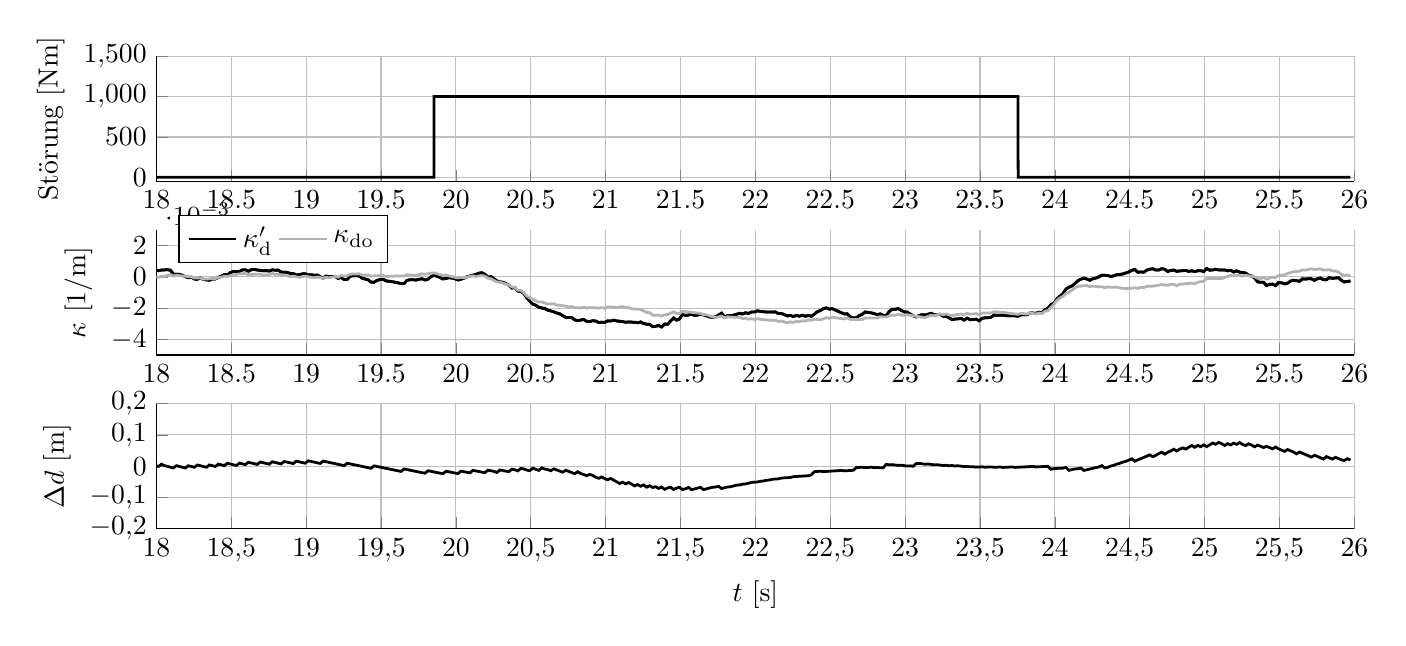
\begin{tikzpicture}

\begin{axis}[%
 /pgf/number format/.cd,
        use comma,
        1000 sep={},
width=0.95092\figurewidth,
height=0.264706\figureheight,
at={(0\figurewidth,0\figureheight)},
scale only axis,
every outer x axis line/.append style={black},
every x tick label/.append style={font=\color{black}},
xmin=18,
xmax=26,
xlabel={$t$ [s]},
xlabel near ticks,
xmajorgrids,
every outer y axis line/.append style={black},
every y tick label/.append style={font=\color{black}},
ymin=-0.2,
ymax=0.2,
ylabel={$\Delta d\text{ [m]}$},
ylabel near ticks,
ymajorgrids,
axis x line*=bottom,
axis y line*=left
]
\addplot [color=black,solid,forget plot, line width=1.0]
  table[row sep=crcr]{%
17.97375	0.00420802084173699\\
17.99375	0.00161599053053685\\
18.01375	-0.00096614106169346\\
18.03375	0.00629452986805701\\
18.05375	0.00191130067663581\\
18.07375	-0.000641930319537742\\
18.09375	-0.00318531310096226\\
18.11375	-0.00571914930865969\\
18.13375	0.00158919981364258\\
18.15375	-0.000925437397504947\\
18.17375	-0.00343066310150153\\
18.19375	-0.00592649052508554\\
18.21275	0.00141968150186633\\
18.23375	-0.00105735099733373\\
18.25375	-0.00352513564015355\\
18.27375	0.00384878148078593\\
18.29375	0.0013995121263255\\
18.31375	-0.00104066364470556\\
18.33375	-0.00347154597796084\\
18.35375	0.00393861406876184\\
18.37375	0.001525601092637\\
18.39375	-0.000878264065052647\\
18.41375	0.00655860661505203\\
18.43375	0.00417230357945853\\
18.45375	0.00179498863803884\\
18.47375	0.00925810684766493\\
18.49375	0.00689804818621065\\
18.51375	0.0045468067674248\\
18.53375	0.00220409408866606\\
18.55475	0.00970140389891805\\
18.57375	0.00737575244946109\\
18.59375	0.00505847566569351\\
18.61375	0.0125809119154026\\
18.63375	0.010280356617741\\
18.65375	0.00798801828011486\\
18.67375	0.00570381251178231\\
18.69375	0.0132591203314165\\
18.71375	0.0109912133030106\\
18.73375	0.00873126914679956\\
18.75375	0.00647944115971955\\
18.77375	0.0140665239901598\\
18.79375	0.0118303221003906\\
18.81275	0.00960205042599416\\
18.83275	0.00738148832112895\\
18.85375	0.0149993991681288\\
18.87375	0.0127941533101432\\
18.89375	0.0105964464561792\\
18.91375	0.00840617591874526\\
18.93375	0.016054144501771\\
18.95375	0.0138787513965157\\
18.97375	0.0117106139346177\\
18.99375	0.00954984678895521\\
19.01375	0.0172267670570156\\
19.03375	0.0150802113004977\\
19.05375	0.0129408305685472\\
19.07375	0.0108084474338375\\
19.09375	0.0086829513099298\\
19.11375	0.016394749027512\\
19.13375	0.0142830109816918\\
19.15375	0.0121779725643498\\
19.17375	0.0100797244182682\\
19.19375	0.00798809715153448\\
19.21375	0.00590297988635768\\
19.23375	0.00382446306821116\\
19.25375	0.00175237000382422\\
19.27375	0.00951660191001036\\
19.29375	0.00745719210645035\\
19.31375	0.00540401880677699\\
19.33375	0.00335697127836054\\
19.35475	0.00131612816299898\\
19.37375	-0.000718678634872294\\
19.39375	-0.00274755427715379\\
19.41375	-0.00477042081758539\\
19.43275	-0.0067874523685294\\
19.45375	0.0010309420692951\\
19.47375	-0.000974581930611063\\
19.49375	-0.00297446295972614\\
19.51375	-0.00496880573031255\\
19.53375	-0.00695754406029048\\
19.55375	-0.00894084292314856\\
19.57375	-0.0109188018268354\\
19.59375	-0.0128913557669694\\
19.61375	-0.0148586744368751\\
19.63375	-0.0168208523821169\\
19.65375	-0.00894845544504674\\
19.67375	-0.0109004248989724\\
19.69375	-0.0128474533347842\\
19.71375	-0.014789487412203\\
19.73375	-0.016726687172135\\
19.75375	-0.0186591465741932\\
19.77375	-0.0205868139154894\\
19.79375	-0.0225098526570795\\
19.81375	-0.014599199157812\\
19.83375	-0.0165131410373807\\
19.85375	-0.0184226519110373\\
19.87375	-0.0203278247454914\\
19.89375	-0.022228619335027\\
19.91375	-0.0241251890095335\\
19.93375	-0.0161886203997366\\
19.95375	-0.018076907726702\\
19.97375	-0.019961168506013\\
19.99375	-0.0218414943084873\\
20.01375	-0.0237178560385831\\
20.03375	-0.0157615124534005\\
20.05375	-0.0176303397338167\\
20.07375	-0.0194954127944773\\
20.09375	-0.0213568636849431\\
20.11375	-0.013385980353434\\
20.13375	-0.0152403723214452\\
20.15475	-0.0170913406707429\\
20.17275	-0.0189389771944017\\
20.19375	-0.0207832714951834\\
20.21375	-0.0127956440969959\\
20.23375	-0.0146336042158413\\
20.25375	-0.016468429637333\\
20.27375	-0.0201435078525685\\
20.29375	-0.0121438282148798\\
20.31375	-0.0139698939132944\\
20.33375	-0.0157931069247819\\
20.35375	-0.0176135843375165\\
20.37375	-0.00960279106662432\\
20.39375	-0.0114179282181053\\
20.41375	-0.0150743878226072\\
20.43375	-0.00705605410665111\\
20.45375	-0.00886377814175177\\
20.47375	-0.0125132434870214\\
20.49375	-0.0143164076115201\\
20.51375	-0.00628883576354911\\
20.53375	-0.00993186800731971\\
20.55375	-0.0135729295560894\\
20.57375	-0.00553923418649838\\
20.59375	-0.00917644477360779\\
20.61375	-0.0109673316506664\\
20.63375	-0.0146009648692336\\
20.65375	-0.00840452528772229\\
20.67375	-0.012034840859751\\
20.69375	-0.0156635988379388\\
20.71375	-0.0192908564592642\\
20.73375	-0.0130883134143227\\
20.75375	-0.0167127275625707\\
20.77375	-0.0203358053164591\\
20.79375	-0.0239576118068259\\
20.81375	-0.0177498770959161\\
20.83275	-0.023214344531679\\
20.85375	-0.0268326917788246\\
20.87375	-0.0304499890704473\\
20.89375	-0.0260831250952509\\
20.91375	-0.0296985266416274\\
20.93375	-0.0351582289159653\\
20.95475	-0.0387719321006981\\
20.97375	-0.0344018124729533\\
20.99375	-0.0398592992096147\\
21.01375	-0.0434708786836611\\
21.03375	-0.0390988698351404\\
21.05375	-0.0445546044414828\\
21.07375	-0.0500098583702226\\
21.09375	-0.0554646760329049\\
21.11375	-0.0510908515180457\\
21.13375	-0.0565449524290216\\
21.15375	-0.0521705111367234\\
21.17375	-0.0576240862668715\\
21.19375	-0.0630774685670845\\
21.21375	-0.0587024531738809\\
21.23375	-0.064155590973717\\
21.25375	-0.0597804246476401\\
21.27375	-0.0670788969374723\\
21.29375	-0.0627037619602717\\
21.31375	-0.0681569622366034\\
21.33375	-0.0656274216506754\\
21.35375	-0.07108091825986\\
21.37375	-0.0667063766164859\\
21.39375	-0.0740057113126005\\
21.41375	-0.0696317221446194\\
21.43375	-0.0671034152530101\\
21.45375	-0.0744037335372325\\
21.47375	-0.070030879419932\\
21.49275	-0.0675037898681428\\
21.51275	-0.0748054509043659\\
21.53375	-0.0722793578597218\\
21.55375	-0.0679085779057944\\
21.57375	-0.0752119333596162\\
21.59375	-0.0726876379222152\\
21.61375	-0.0701640083195745\\
21.63375	-0.067641080808087\\
21.65375	-0.0749471951807816\\
21.67375	-0.072425785104631\\
21.69375	-0.0699051848616263\\
21.71375	-0.0673854297089722\\
21.73375	-0.0667115562869163\\
21.75475	-0.0641935632264388\\
21.77375	-0.0715048539678129\\
21.79375	-0.0689887971703631\\
21.81375	-0.0664737563208053\\
21.83375	-0.0658046011021116\\
21.85375	-0.0632916545215378\\
21.87375	-0.0607798222422984\\
21.89375	-0.0601138564765376\\
21.91375	-0.0576043090551064\\
21.93375	-0.0569406079545773\\
21.95375	-0.0544334686990688\\
21.97375	-0.0519276011733774\\
21.99375	-0.0512675397889333\\
22.01375	-0.0506087188732733\\
22.03375	-0.0481067561167223\\
22.05375	-0.0474505459709089\\
22.07375	-0.0449513465862346\\
22.09375	-0.0442978577758431\\
22.11375	-0.0418015351490206\\
22.13275	-0.0411508757862338\\
22.15375	-0.0405016441757371\\
22.17375	-0.0380098164544469\\
22.19375	-0.0373635708402005\\
22.21375	-0.0367188368359406\\
22.23375	-0.0360756402253175\\
22.25375	-0.0335901541408883\\
22.27375	-0.0329501437344746\\
22.29375	-0.0323117330522464\\
22.31375	-0.0316749450764049\\
22.33375	-0.0310398024801035\\
22.35375	-0.0304063276254771\\
22.37375	-0.027931066757489\\
22.39375	-0.0174724339970855\\
22.41375	-0.0168441459869104\\
22.43375	-0.0162176126785667\\
22.45375	-0.01743610158689\\
22.47375	-0.0168130943056908\\
22.49375	-0.0161919027959119\\
22.51375	-0.0155725468662151\\
22.53375	-0.0149550460003751\\
22.55475	-0.0143394193559039\\
22.57375	-0.0137256857624166\\
22.59375	-0.0149566177837266\\
22.61375	-0.01434666295888\\
22.63375	-0.0137386687607748\\
22.65375	-0.0131326393794966\\
22.67375	-0.0045422824730057\\
22.69375	-0.00394014561342404\\
22.71375	-0.00334002332768124\\
22.73375	-0.00458419390438713\\
22.75275	-0.0039880727574122\\
22.77375	-0.0033940273920523\\
22.79375	-0.00464412670742576\\
22.81375	-0.00405418248001066\\
22.83375	-0.0053082456227993\\
22.85375	-0.00472244818129131\\
22.87375	0.00569015203574086\\
22.89375	0.00443002109786628\\
22.91375	0.00500945386981044\\
22.93275	0.00374518022132264\\
22.95375	0.0024788842869623\\
22.97375	0.00305192214852212\\
22.99375	0.00178146788383948\\
23.01375	0.000508959773844797\\
23.03375	0.00107548400206792\\
23.05375	-0.00020129842036809\\
23.07375	0.00834891489897371\\
23.09375	0.00890886960176474\\
23.11375	0.00762574317276599\\
23.13375	0.00634050328386282\\
23.15375	0.00689376668061792\\
23.17375	0.00560414907815909\\
23.19375	0.0043123990454732\\
23.21375	0.0048589241913124\\
23.23375	0.0035628027279726\\
23.25375	0.00226452188579396\\
23.27375	0.00280421734395508\\
23.29375	0.00150147698133463\\
23.31375	0.00203657723843031\\
23.33175	0.000729404300361391\\
23.35475	0.00125988749266615\\
23.37375	-5.17376796089764e-005\\
23.39375	-0.00136558857939484\\
23.41375	-0.000842049895832364\\
23.43375	-0.00216039780413801\\
23.45375	-0.00164151873170715\\
23.47375	-0.00296435646252835\\
23.49375	-0.00245014906718888\\
23.51375	-0.00193832535245742\\
23.53375	-0.00326799842703007\\
23.55375	-0.00276088737285507\\
23.57375	-0.0022561649583972\\
23.59375	-0.00359266905649003\\
23.61375	-0.00309263771288038\\
23.63375	-0.00259499663094509\\
23.65375	-0.00393831685899082\\
23.67375	-0.0034453761405997\\
23.69375	-0.00295484273568203\\
23.71375	-0.00246669659096765\\
23.73375	-0.0038191829070322\\
23.75375	-0.00333571754657402\\
23.77375	-0.00285463335228808\\
23.79375	-0.0023759275256654\\
23.81375	-0.00189959689388619\\
23.83375	-0.00142563791023109\\
23.85375	-0.00095405379404756\\
23.87375	-0.00232251427672603\\
23.89375	-0.00185558544137177\\
23.91375	-0.00139101039241218\\
23.93275	-0.000928783717829784\\
23.95375	-0.000468899633440323\\
23.97375	-0.00984113328234004\\
23.99375	-0.0075487917789232\\
24.01375	-0.00709599902158464\\
24.03375	-0.00664552166151244\\
24.05375	-0.00619735204339822\\
24.07375	-0.00391468416411778\\
24.09375	-0.0133010857605402\\
24.11375	-0.0110232594096171\\
24.13375	-0.00874787401334798\\
24.15475	-0.0083114081628346\\
24.17375	-0.00604078900288219\\
24.19375	-0.013602528062679\\
24.21375	-0.011336728767084\\
24.23375	-0.00907331335847728\\
24.25375	-0.00681226910430066\\
24.27375	-0.00455358285388785\\
24.29375	-0.00229724104042894\\
24.31375	0.00179260285944727\\
24.33375	-0.00578584395938941\\
24.35375	-0.00353654515438118\\
24.37375	0.000546039120619568\\
24.39375	0.00279070484826294\\
24.41375	0.00686853295936096\\
24.43375	0.00910863209740764\\
24.45375	0.0131817745160938\\
24.47375	0.0154173769611425\\
24.49375	0.0194859076640679\\
24.51375	0.0235521241497798\\
24.53275	0.0159508792611209\\
24.55375	0.0200125885124356\\
24.57375	0.0240720456648678\\
24.59375	0.0281292724887954\\
24.61375	0.0321842780075716\\
24.63375	0.0362370869656772\\
24.65375	0.0304574459992448\\
24.67375	0.0345059419836398\\
24.69375	0.0403866999381375\\
24.71375	0.04443092485129\\
24.73375	0.0386427471668052\\
24.75375	0.0445170199784064\\
24.77375	0.0485550295480657\\
24.79375	0.0544250812166207\\
24.81375	0.0486286931949138\\
24.83375	0.0544946556904335\\
24.85375	0.058524750493731\\
24.87375	0.0545563139247487\\
24.89375	0.0604162992446038\\
24.91375	0.0662743519356321\\
24.93375	0.0604664554746388\\
24.95475	0.0663207844349065\\
24.97375	0.0623427827407639\\
24.99375	0.0681934246689226\\
25.01375	0.0623784423737725\\
25.03375	0.0682256233392895\\
25.05375	0.0740711031851022\\
25.07375	0.0700843721398998\\
25.09375	0.0759265125065984\\
25.11375	0.0719365044558207\\
25.13375	0.0661118834189303\\
25.15375	0.0719493791618957\\
25.17375	0.0679547970919243\\
25.19375	0.0737893224280408\\
25.21375	0.0697918403272184\\
25.23375	0.0756235784926562\\
25.25275	0.0697906042209926\\
25.27375	0.0657891143085978\\
25.29375	0.071616971442598\\
25.31375	0.0676129775936491\\
25.33375	0.061775190138313\\
25.35375	0.067599546718013\\
25.37375	0.0635921404131836\\
25.39375	0.0595836597033768\\
25.41375	0.0635723591193438\\
25.43375	0.0595619125090328\\
25.45375	0.0555505281904805\\
25.47375	0.0613689220704634\\
25.49375	0.0555234264541871\\
25.51375	0.0515095001072763\\
25.53375	0.0474948100760431\\
25.55375	0.0533101040315294\\
25.57375	0.0492940121649199\\
25.59375	0.0452772885302304\\
25.61375	0.0394277572279895\\
25.63375	0.0452406454650385\\
25.65375	0.0412223250136798\\
25.67375	0.0372035481245403\\
25.69375	0.0331843709715556\\
25.71375	0.0291648405827929\\
25.73375	0.0349757328205498\\
25.75475	0.0309556351889095\\
25.77375	0.0269353245409336\\
25.79375	0.0229148509352912\\
25.81375	0.0305571211371967\\
25.83375	0.0265364636365675\\
25.85375	0.0225157896825992\\
25.87375	0.0283258813713774\\
25.89375	0.0243053205561194\\
25.91375	0.0202848904168391\\
25.93275	0.0180967853085376\\
25.95375	0.0239075049479811\\
25.97375	0.0198877751002047\\
};
\end{axis}

\begin{axis}[%
width=0.95092\figurewidth,
height=0.264706\figureheight,
at={(0\figurewidth,0.367647\figureheight)},
scale only axis,
every outer x axis line/.append style={black},
every x tick label/.append style={font=\color{black}},
xmin=18,
xmax=26,
xmajorgrids,
every outer y axis line/.append style={black},
every y tick label/.append style={font=\color{black}},
ymin=-0.005,
ymax=0.003,
ylabel={$\kappa\text{ [1/m]}$},
ylabel near ticks,
ymajorgrids,
axis x line*=bottom,
axis y line*=left,
legend style={at={(0.018413,0.734139)},anchor=south west,legend columns=2,legend cell align=left,align=left,draw=black}
]
\addplot [color=black,solid, line width=1.0]
  table[row sep=crcr]{%
17.97375	0.000323821473980823\\
17.99375	0.00045161412906528\\
18.01375	0.000399209081593525\\
18.03375	0.000434593753106015\\
18.05375	0.000445119855728241\\
18.07375	0.00045756984332177\\
18.09375	0.000429477955209978\\
18.11375	0.000180056749310244\\
18.13375	0.000162682145702333\\
18.15375	0.000158315521384546\\
18.17375	0.000100027752142495\\
18.19375	9.75916267243263e-006\\
18.21275	-5.94942101145908e-005\\
18.23375	-2.02311436937398e-005\\
18.25375	-0.000139222986038058\\
18.27375	-0.000152647108222784\\
18.29375	-7.28141781894108e-005\\
18.31375	-0.000163327018777421\\
18.33375	-0.000195235817850069\\
18.35375	-0.000216272828693524\\
18.37375	-0.000139692987940828\\
18.39375	-0.000131617058448218\\
18.41375	-3.36206007454451e-005\\
18.43375	4.47913983356136e-005\\
18.45375	0.000140963477348756\\
18.47375	0.00011884394050142\\
18.49375	0.000273287255974575\\
18.51375	0.000340368666405241\\
18.53375	0.000346826265890152\\
18.55475	0.000350545902230609\\
18.57375	0.000441789863853653\\
18.59375	0.00045727860726829\\
18.61375	0.000362771116426865\\
18.63375	0.000456023119103066\\
18.65375	0.000472649775070843\\
18.67375	0.000439883336101985\\
18.69375	0.000414973701032743\\
18.71375	0.000389294512630722\\
18.73375	0.000399832083636455\\
18.75375	0.00036870166207992\\
18.77375	0.000447529635901847\\
18.79375	0.000423521561929034\\
18.81275	0.000434959545408876\\
18.83275	0.000306671407049181\\
18.85375	0.000294851605316549\\
18.87375	0.000286700364880953\\
18.89375	0.000218514111576058\\
18.91375	0.000212822214341372\\
18.93375	0.000122140998494146\\
18.95375	0.000136761433785597\\
18.97375	0.000189285978879197\\
18.99375	0.000198382119548506\\
19.01375	0.000118604128106723\\
19.03375	0.000140437608716426\\
19.05375	9.89756761014846e-005\\
19.07375	0.000117324041604288\\
19.09375	8.70774333736118e-006\\
19.11375	-7.57457174859962e-005\\
19.13375	4.88013889473028e-005\\
19.15375	1.00284271825252e-005\\
19.17375	3.05019906929371e-005\\
19.19375	2.24477450129483e-005\\
19.21375	-0.000100764132413352\\
19.23375	-3.31758302723329e-005\\
19.25375	-0.000172711951899935\\
19.27375	-0.000175637436733794\\
19.29375	3.36527251024043e-005\\
19.31375	7.83675025637052e-005\\
19.33375	7.97356307252351e-005\\
19.35475	5.29302991310901e-005\\
19.37375	-8.90579001756781e-005\\
19.39375	-0.000136495235443338\\
19.41375	-0.000186631073634458\\
19.43275	-0.000335077311152974\\
19.45375	-0.00034018442078567\\
19.47375	-0.000227481230779736\\
19.49375	-0.000171394983312633\\
19.51375	-0.000154176777073436\\
19.53375	-0.000261048893083489\\
19.55375	-0.000280561860464454\\
19.57375	-0.000308955209667207\\
19.59375	-0.00034408002722953\\
19.61375	-0.000383770584746879\\
19.63375	-0.0004258480491716\\
19.65375	-0.000430972843209058\\
19.67375	-0.00022399409233144\\
19.69375	-0.000180957181531054\\
19.71375	-0.000180304258903954\\
19.73375	-0.000207928175852328\\
19.75375	-0.00015634678906037\\
19.77375	-0.00012276926888089\\
19.79375	-0.000201692149281296\\
19.81375	-0.000150530644718124\\
19.83375	6.76014071551497e-006\\
19.85375	9.6970207476391e-005\\
19.87375	4.30820787931635e-005\\
19.89375	-3.85432456040216e-005\\
19.91375	-0.000134545928354282\\
19.93375	-0.000100525061895634\\
19.95375	-5.68605793210454e-005\\
19.97375	-7.17471632411205e-005\\
19.99375	-0.000125007907298938\\
20.01375	-0.000199176453987034\\
20.03375	-0.000147694619098311\\
20.05375	-8.95386096327253e-005\\
20.07375	4.94573424291097e-006\\
20.09375	5.43784453360826e-005\\
20.11375	0.000109832986858582\\
20.13375	0.000158836452253588\\
20.15475	0.000236925732392618\\
20.17275	0.000265600719654958\\
20.19375	0.000162315141543912\\
20.21375	-1.71093094290202e-005\\
20.23375	1.59704752620531e-005\\
20.25375	-0.000105690192223767\\
20.27375	-0.000262969819497784\\
20.29375	-0.000317286016729836\\
20.31375	-0.000349947319290289\\
20.33375	-0.000429817246776707\\
20.35375	-0.000536366249997246\\
20.37375	-0.000715467866698612\\
20.39375	-0.000678601356612284\\
20.41375	-0.000902696239761023\\
20.43375	-0.00093786257901036\\
20.45375	-0.0010615598354044\\
20.47375	-0.00134183385598381\\
20.49375	-0.00156488980526758\\
20.51375	-0.00174737846784415\\
20.53375	-0.00180937362651304\\
20.55375	-0.00194920543529313\\
20.57375	-0.00199023444176454\\
20.59375	-0.00202308634283124\\
20.61375	-0.00213516698950846\\
20.63375	-0.00217844223409183\\
20.65375	-0.00223805821487355\\
20.67375	-0.00231180197161561\\
20.69375	-0.00236680071906846\\
20.71375	-0.00247894455603672\\
20.73375	-0.00258951184716443\\
20.75375	-0.00260509301863177\\
20.77375	-0.00260136061502081\\
20.79375	-0.0027543649585232\\
20.81375	-0.002801278595139\\
20.83275	-0.00276282235567111\\
20.85375	-0.00272888390044452\\
20.87375	-0.00284587730514393\\
20.89375	-0.00286121847512024\\
20.91375	-0.00280378535957563\\
20.93375	-0.00282466917410288\\
20.95475	-0.00291899050677228\\
20.97375	-0.00290210031655685\\
20.99375	-0.0029166366546577\\
21.01375	-0.00281388964436419\\
21.03375	-0.00282409989934914\\
21.05375	-0.00277079537991434\\
21.07375	-0.00282127212504977\\
21.09375	-0.00283725841705991\\
21.11375	-0.00286444297304743\\
21.13375	-0.00290390358148723\\
21.15375	-0.00288081113152738\\
21.17375	-0.00289466470816514\\
21.19375	-0.00290405546436051\\
21.21375	-0.00293796361147142\\
21.23375	-0.00288528576330111\\
21.25375	-0.00298850959545578\\
21.27375	-0.00302517510169915\\
21.29375	-0.00303931396188964\\
21.31375	-0.00318372354083798\\
21.33375	-0.00316660945537203\\
21.35375	-0.00310890329871395\\
21.37375	-0.00320467456586801\\
21.39375	-0.0030176066587292\\
21.41375	-0.00303116452045752\\
21.43375	-0.00282692109798413\\
21.45375	-0.00263186174655712\\
21.47375	-0.0027687962596189\\
21.49275	-0.00269166200713433\\
21.51275	-0.00240923710455829\\
21.53375	-0.002468978924594\\
21.55375	-0.00244006572911617\\
21.57375	-0.00239276058360241\\
21.59375	-0.00246221988442664\\
21.61375	-0.00245055592318001\\
21.63375	-0.00238661885103895\\
21.65375	-0.00243921857089237\\
21.67375	-0.00249369763786234\\
21.69375	-0.00256672981253389\\
21.71375	-0.00258418916909743\\
21.73375	-0.00256801054152027\\
21.75475	-0.00243950020031596\\
21.77375	-0.00232797899892127\\
21.79375	-0.00255974997561125\\
21.81375	-0.00248385976502981\\
21.83375	-0.00247319984559621\\
21.85375	-0.00245321153214046\\
21.87375	-0.00239862947682175\\
21.89375	-0.0023278630578567\\
21.91375	-0.00237760489533707\\
21.93375	-0.00229904326457157\\
21.95375	-0.00233949604509737\\
21.97375	-0.00224448388315604\\
21.99375	-0.0022509254867907\\
22.01375	-0.00217266777843822\\
22.03375	-0.0022125335107947\\
22.05375	-0.00222905196239842\\
22.07375	-0.00225043335292683\\
22.09375	-0.00225039873950624\\
22.11375	-0.00225529349722467\\
22.13275	-0.00223854542775768\\
22.15375	-0.00235002303364477\\
22.17375	-0.00234183447985816\\
22.19375	-0.00241668158946598\\
22.21375	-0.00249756625566407\\
22.23375	-0.00246584030388298\\
22.25375	-0.00253695010054124\\
22.27375	-0.00246401411199097\\
22.29375	-0.00251512184032746\\
22.31375	-0.00245954704571414\\
22.33375	-0.00252093420268292\\
22.35375	-0.00246924971489825\\
22.37375	-0.00252237976003563\\
22.39375	-0.00238459511940376\\
22.41375	-0.00222780060816951\\
22.43375	-0.00215565833108032\\
22.45375	-0.00203607813739035\\
22.47375	-0.00198647893802207\\
22.49375	-0.00206482824057716\\
22.51375	-0.00203597040155152\\
22.53375	-0.00212503431577072\\
22.55475	-0.0022114791067897\\
22.57375	-0.00229231994322249\\
22.59375	-0.00237406370277061\\
22.61375	-0.00236355265670791\\
22.63375	-0.0025592481012526\\
22.65375	-0.00261576835105801\\
22.67375	-0.00261435396732459\\
22.69375	-0.00247645359180749\\
22.71375	-0.00239331846780674\\
22.73375	-0.00224454453566857\\
22.75275	-0.00227326053692674\\
22.77375	-0.00230453891415206\\
22.79375	-0.0023465800952959\\
22.81375	-0.00241829992239668\\
22.83375	-0.00236982351231996\\
22.85375	-0.00245905349557895\\
22.87375	-0.00247574158799415\\
22.89375	-0.00221917446168961\\
22.91375	-0.00206514520708224\\
22.93275	-0.00207451541645559\\
22.95375	-0.00203220827819631\\
22.97375	-0.00213953794457727\\
22.99375	-0.00223980912063164\\
23.01375	-0.00225029407087832\\
23.03375	-0.00238375298826537\\
23.05375	-0.00249182205274264\\
23.07375	-0.00255976256561542\\
23.09375	-0.00246543196318904\\
23.11375	-0.0024206999871339\\
23.13375	-0.00244604853193489\\
23.15375	-0.0023853714834159\\
23.17375	-0.00232938870699695\\
23.19375	-0.00242660153882729\\
23.21375	-0.00241725990435068\\
23.23375	-0.00239566136541274\\
23.25375	-0.00251416590522366\\
23.27375	-0.00252122925673683\\
23.29375	-0.00262443806374023\\
23.31375	-0.00273418107606645\\
23.33175	-0.00270251327788349\\
23.35475	-0.00268485937600365\\
23.37375	-0.00265382232815122\\
23.39375	-0.00276207655252082\\
23.41375	-0.00264190472995799\\
23.43375	-0.00273994372032036\\
23.45375	-0.00272997741134997\\
23.47375	-0.00270447022082425\\
23.49375	-0.00280923290953783\\
23.51375	-0.00265529711504313\\
23.53375	-0.00261892354341589\\
23.55375	-0.00260842981766129\\
23.57375	-0.00258301217911086\\
23.59375	-0.00244509571336911\\
23.61375	-0.00245513439195081\\
23.63375	-0.00245310693349064\\
23.65375	-0.0024540645415044\\
23.67375	-0.00248056829685377\\
23.69375	-0.00249088858757041\\
23.71375	-0.00249127728733057\\
23.73375	-0.0024948787812187\\
23.75375	-0.00252373770645726\\
23.77375	-0.00242124296452652\\
23.79375	-0.00242792209739422\\
23.81375	-0.00242957048099189\\
23.83375	-0.0023141483695082\\
23.85375	-0.00231754531194331\\
23.87375	-0.00233167399900701\\
23.89375	-0.00226107134148708\\
23.91375	-0.00229598202246269\\
23.93275	-0.00209735183925201\\
23.95375	-0.00201785056091119\\
23.97375	-0.00177316510202208\\
23.99375	-0.00169045879731229\\
24.01375	-0.00141199124367529\\
24.03375	-0.0012392586036165\\
24.05375	-0.00107084087573005\\
24.07375	-0.000789286685981336\\
24.09375	-0.000660338661701205\\
24.11375	-0.000587988623384013\\
24.13375	-0.000429579520122222\\
24.15475	-0.000236627942679273\\
24.17375	-0.000151460220940395\\
24.19375	-7.76600936107245e-005\\
24.21375	-0.000139858313938592\\
24.23375	-0.000218477477458518\\
24.25375	-0.000116699515724949\\
24.27375	-7.62090646837579e-005\\
24.29375	-2.80676250000189e-007\\
24.31375	0.000103498989968883\\
24.33375	0.000101417923033581\\
24.35375	7.76706962365598e-005\\
24.37375	2.90870227995424e-005\\
24.39375	6.60704535209348e-005\\
24.41375	0.000141173164562945\\
24.43375	0.00015559446147936\\
24.45375	0.000184229688060798\\
24.47375	0.000247003240572216\\
24.49375	0.000313403026644311\\
24.51375	0.000413080616349436\\
24.53275	0.000478896789640639\\
24.55375	0.000293634934129457\\
24.57375	0.000315586487662916\\
24.59375	0.00029686351924079\\
24.61375	0.000431344751727054\\
24.63375	0.000487094552950158\\
24.65375	0.000518675534878985\\
24.67375	0.000434359424619038\\
24.69375	0.000440095827122616\\
24.71375	0.000524060544901119\\
24.73375	0.000484569026725949\\
24.75375	0.000343609679827388\\
24.77375	0.000414669226143357\\
24.79375	0.000432453184698093\\
24.81375	0.000353369866336333\\
24.83375	0.000380518342477067\\
24.85375	0.000395182394451402\\
24.87375	0.000409226747948122\\
24.89375	0.000350522808301341\\
24.91375	0.000390184059280244\\
24.93375	0.000339498956451529\\
24.95475	0.000392026488954283\\
24.97375	0.000397001458849489\\
24.99375	0.000339500674580071\\
25.01375	0.000534750819528195\\
25.03375	0.000427594539442169\\
25.05375	0.000442602861748597\\
25.07375	0.000484451050742458\\
25.09375	0.000444693290986896\\
25.11375	0.00044653166395918\\
25.13375	0.000442156742684429\\
25.15375	0.000387699440962677\\
25.17375	0.000422872758135832\\
25.19375	0.000308142672720352\\
25.21375	0.000382530078582161\\
25.23375	0.000302618872766323\\
25.25275	0.000279494290951488\\
25.27375	0.000241568192815934\\
25.29375	0.000102915984848561\\
25.31375	6.01369907256662e-005\\
25.33375	-7.18440608481656e-005\\
25.35375	-0.000320119865237572\\
25.37375	-0.000350538820761782\\
25.39375	-0.00034861432921719\\
25.41375	-0.000555754136001189\\
25.43375	-0.00047345524448526\\
25.45375	-0.000463807534672573\\
25.47375	-0.000557440971237212\\
25.49375	-0.000362399435651973\\
25.51375	-0.000384305442581676\\
25.53375	-0.000449069544550439\\
25.55375	-0.000406441157596343\\
25.57375	-0.000269035019867403\\
25.59375	-0.000219391118246141\\
25.61375	-0.000239995342265097\\
25.63375	-0.000285626342997826\\
25.65375	-0.000124005251971827\\
25.67375	-0.000145003911010797\\
25.69375	-0.00011620908858934\\
25.71375	-0.000127241605756966\\
25.73375	-0.000226173188475251\\
25.75475	-0.000112533452632019\\
25.77375	-7.43371729986891e-005\\
25.79375	-0.000189126594918143\\
25.81375	-0.000180916328910701\\
25.83375	-4.71907400696992e-005\\
25.85375	-0.000103487928654826\\
25.87375	-7.1279707641639e-005\\
25.89375	-5.60636309245096e-005\\
25.91375	-0.000223286890643139\\
25.93275	-0.000325539709302636\\
25.95375	-0.000290537786726986\\
25.97375	-0.000266694459689462\\
};
\addlegendentry{$\kappa{}_\mathrm{d}'$};



\addplot [color=black,solid,forget plot, line width=1.0]
  table[row sep=crcr]{%
17.97375	0.000323821473980823\\
17.99375	0.00045161412906528\\
18.01375	0.000399209081593525\\
18.03375	0.000434593753106015\\
18.05375	0.000445119855728241\\
18.07375	0.00045756984332177\\
18.09375	0.000429477955209978\\
18.11375	0.000180056749310244\\
18.13375	0.000162682145702333\\
18.15375	0.000158315521384546\\
18.17375	0.000100027752142495\\
18.19375	9.75916267243263e-006\\
18.21275	-5.94942101145908e-005\\
18.23375	-2.02311436937398e-005\\
18.25375	-0.000139222986038058\\
18.27375	-0.000152647108222784\\
18.29375	-7.28141781894108e-005\\
18.31375	-0.000163327018777421\\
18.33375	-0.000195235817850069\\
18.35375	-0.000216272828693524\\
18.37375	-0.000139692987940828\\
18.39375	-0.000131617058448218\\
18.41375	-3.36206007454451e-005\\
18.43375	4.47913983356136e-005\\
18.45375	0.000140963477348756\\
18.47375	0.00011884394050142\\
18.49375	0.000273287255974575\\
18.51375	0.000340368666405241\\
18.53375	0.000346826265890152\\
18.55475	0.000350545902230609\\
18.57375	0.000441789863853653\\
18.59375	0.00045727860726829\\
18.61375	0.000362771116426865\\
18.63375	0.000456023119103066\\
18.65375	0.000472649775070843\\
18.67375	0.000439883336101985\\
18.69375	0.000414973701032743\\
18.71375	0.000389294512630722\\
18.73375	0.000399832083636455\\
18.75375	0.00036870166207992\\
18.77375	0.000447529635901847\\
18.79375	0.000423521561929034\\
18.81275	0.000434959545408876\\
18.83275	0.000306671407049181\\
18.85375	0.000294851605316549\\
18.87375	0.000286700364880953\\
18.89375	0.000218514111576058\\
18.91375	0.000212822214341372\\
18.93375	0.000122140998494146\\
18.95375	0.000136761433785597\\
18.97375	0.000189285978879197\\
18.99375	0.000198382119548506\\
19.01375	0.000118604128106723\\
19.03375	0.000140437608716426\\
19.05375	9.89756761014846e-005\\
19.07375	0.000117324041604288\\
19.09375	8.70774333736118e-006\\
19.11375	-7.57457174859962e-005\\
19.13375	4.88013889473028e-005\\
19.15375	1.00284271825252e-005\\
19.17375	3.05019906929371e-005\\
19.19375	2.24477450129483e-005\\
19.21375	-0.000100764132413352\\
19.23375	-3.31758302723329e-005\\
19.25375	-0.000172711951899935\\
19.27375	-0.000175637436733794\\
19.29375	3.36527251024043e-005\\
19.31375	7.83675025637052e-005\\
19.33375	7.97356307252351e-005\\
19.35475	5.29302991310901e-005\\
19.37375	-8.90579001756781e-005\\
19.39375	-0.000136495235443338\\
19.41375	-0.000186631073634458\\
19.43275	-0.000335077311152974\\
19.45375	-0.00034018442078567\\
19.47375	-0.000227481230779736\\
19.49375	-0.000171394983312633\\
19.51375	-0.000154176777073436\\
19.53375	-0.000261048893083489\\
19.55375	-0.000280561860464454\\
19.57375	-0.000308955209667207\\
19.59375	-0.00034408002722953\\
19.61375	-0.000383770584746879\\
19.63375	-0.0004258480491716\\
19.65375	-0.000430972843209058\\
19.67375	-0.00022399409233144\\
19.69375	-0.000180957181531054\\
19.71375	-0.000180304258903954\\
19.73375	-0.000207928175852328\\
19.75375	-0.00015634678906037\\
19.77375	-0.00012276926888089\\
19.79375	-0.000201692149281296\\
19.81375	-0.000150530644718124\\
19.83375	6.76014071551497e-006\\
19.85375	9.6970207476391e-005\\
19.87375	4.30820787931635e-005\\
19.89375	-3.85432456040216e-005\\
19.91375	-0.000134545928354282\\
19.93375	-0.000100525061895634\\
19.95375	-5.68605793210454e-005\\
19.97375	-7.17471632411205e-005\\
19.99375	-0.000125007907298938\\
20.01375	-0.000199176453987034\\
20.03375	-0.000147694619098311\\
20.05375	-8.95386096327253e-005\\
20.07375	4.94573424291097e-006\\
20.09375	5.43784453360826e-005\\
20.11375	0.000109832986858582\\
20.13375	0.000158836452253588\\
20.15475	0.000236925732392618\\
20.17275	0.000265600719654958\\
20.19375	0.000162315141543912\\
20.21375	-1.71093094290202e-005\\
20.23375	1.59704752620531e-005\\
20.25375	-0.000105690192223767\\
20.27375	-0.000262969819497784\\
20.29375	-0.000317286016729836\\
20.31375	-0.000349947319290289\\
20.33375	-0.000429817246776707\\
20.35375	-0.000536366249997246\\
20.37375	-0.000715467866698612\\
20.39375	-0.000678601356612284\\
20.41375	-0.000902696239761023\\
20.43375	-0.00093786257901036\\
20.45375	-0.0010615598354044\\
20.47375	-0.00134183385598381\\
20.49375	-0.00156488980526758\\
20.51375	-0.00174737846784415\\
20.53375	-0.00180937362651304\\
20.55375	-0.00194920543529313\\
20.57375	-0.00199023444176454\\
20.59375	-0.00202308634283124\\
20.61375	-0.00213516698950846\\
20.63375	-0.00217844223409183\\
20.65375	-0.00223805821487355\\
20.67375	-0.00231180197161561\\
20.69375	-0.00236680071906846\\
20.71375	-0.00247894455603672\\
20.73375	-0.00258951184716443\\
20.75375	-0.00260509301863177\\
20.77375	-0.00260136061502081\\
20.79375	-0.0027543649585232\\
20.81375	-0.002801278595139\\
20.83275	-0.00276282235567111\\
20.85375	-0.00272888390044452\\
20.87375	-0.00284587730514393\\
20.89375	-0.00286121847512024\\
20.91375	-0.00280378535957563\\
20.93375	-0.00282466917410288\\
20.95475	-0.00291899050677228\\
20.97375	-0.00290210031655685\\
20.99375	-0.0029166366546577\\
21.01375	-0.00281388964436419\\
21.03375	-0.00282409989934914\\
21.05375	-0.00277079537991434\\
21.07375	-0.00282127212504977\\
21.09375	-0.00283725841705991\\
21.11375	-0.00286444297304743\\
21.13375	-0.00290390358148723\\
21.15375	-0.00288081113152738\\
21.17375	-0.00289466470816514\\
21.19375	-0.00290405546436051\\
21.21375	-0.00293796361147142\\
21.23375	-0.00288528576330111\\
21.25375	-0.00298850959545578\\
21.27375	-0.00302517510169915\\
21.29375	-0.00303931396188964\\
21.31375	-0.00318372354083798\\
21.33375	-0.00316660945537203\\
21.35375	-0.00310890329871395\\
21.37375	-0.00320467456586801\\
21.39375	-0.0030176066587292\\
21.41375	-0.00303116452045752\\
21.43375	-0.00282692109798413\\
21.45375	-0.00263186174655712\\
21.47375	-0.0027687962596189\\
21.49275	-0.00269166200713433\\
21.51275	-0.00240923710455829\\
21.53375	-0.002468978924594\\
21.55375	-0.00244006572911617\\
21.57375	-0.00239276058360241\\
21.59375	-0.00246221988442664\\
21.61375	-0.00245055592318001\\
21.63375	-0.00238661885103895\\
21.65375	-0.00243921857089237\\
21.67375	-0.00249369763786234\\
21.69375	-0.00256672981253389\\
21.71375	-0.00258418916909743\\
21.73375	-0.00256801054152027\\
21.75475	-0.00243950020031596\\
21.77375	-0.00232797899892127\\
21.79375	-0.00255974997561125\\
21.81375	-0.00248385976502981\\
21.83375	-0.00247319984559621\\
21.85375	-0.00245321153214046\\
21.87375	-0.00239862947682175\\
21.89375	-0.0023278630578567\\
21.91375	-0.00237760489533707\\
21.93375	-0.00229904326457157\\
21.95375	-0.00233949604509737\\
21.97375	-0.00224448388315604\\
21.99375	-0.0022509254867907\\
22.01375	-0.00217266777843822\\
22.03375	-0.0022125335107947\\
22.05375	-0.00222905196239842\\
22.07375	-0.00225043335292683\\
22.09375	-0.00225039873950624\\
22.11375	-0.00225529349722467\\
22.13275	-0.00223854542775768\\
22.15375	-0.00235002303364477\\
22.17375	-0.00234183447985816\\
22.19375	-0.00241668158946598\\
22.21375	-0.00249756625566407\\
22.23375	-0.00246584030388298\\
22.25375	-0.00253695010054124\\
22.27375	-0.00246401411199097\\
22.29375	-0.00251512184032746\\
22.31375	-0.00245954704571414\\
22.33375	-0.00252093420268292\\
22.35375	-0.00246924971489825\\
22.37375	-0.00252237976003563\\
22.39375	-0.00238459511940376\\
22.41375	-0.00222780060816951\\
22.43375	-0.00215565833108032\\
22.45375	-0.00203607813739035\\
22.47375	-0.00198647893802207\\
22.49375	-0.00206482824057716\\
22.51375	-0.00203597040155152\\
22.53375	-0.00212503431577072\\
22.55475	-0.0022114791067897\\
22.57375	-0.00229231994322249\\
22.59375	-0.00237406370277061\\
22.61375	-0.00236355265670791\\
22.63375	-0.0025592481012526\\
22.65375	-0.00261576835105801\\
22.67375	-0.00261435396732459\\
22.69375	-0.00247645359180749\\
22.71375	-0.00239331846780674\\
22.73375	-0.00224454453566857\\
22.75275	-0.00227326053692674\\
22.77375	-0.00230453891415206\\
22.79375	-0.0023465800952959\\
22.81375	-0.00241829992239668\\
22.83375	-0.00236982351231996\\
22.85375	-0.00245905349557895\\
22.87375	-0.00247574158799415\\
22.89375	-0.00221917446168961\\
22.91375	-0.00206514520708224\\
22.93275	-0.00207451541645559\\
22.95375	-0.00203220827819631\\
22.97375	-0.00213953794457727\\
22.99375	-0.00223980912063164\\
23.01375	-0.00225029407087832\\
23.03375	-0.00238375298826537\\
23.05375	-0.00249182205274264\\
23.07375	-0.00255976256561542\\
23.09375	-0.00246543196318904\\
23.11375	-0.0024206999871339\\
23.13375	-0.00244604853193489\\
23.15375	-0.0023853714834159\\
23.17375	-0.00232938870699695\\
23.19375	-0.00242660153882729\\
23.21375	-0.00241725990435068\\
23.23375	-0.00239566136541274\\
23.25375	-0.00251416590522366\\
23.27375	-0.00252122925673683\\
23.29375	-0.00262443806374023\\
23.31375	-0.00273418107606645\\
23.33175	-0.00270251327788349\\
23.35475	-0.00268485937600365\\
23.37375	-0.00265382232815122\\
23.39375	-0.00276207655252082\\
23.41375	-0.00264190472995799\\
23.43375	-0.00273994372032036\\
23.45375	-0.00272997741134997\\
23.47375	-0.00270447022082425\\
23.49375	-0.00280923290953783\\
23.51375	-0.00265529711504313\\
23.53375	-0.00261892354341589\\
23.55375	-0.00260842981766129\\
23.57375	-0.00258301217911086\\
23.59375	-0.00244509571336911\\
23.61375	-0.00245513439195081\\
23.63375	-0.00245310693349064\\
23.65375	-0.0024540645415044\\
23.67375	-0.00248056829685377\\
23.69375	-0.00249088858757041\\
23.71375	-0.00249127728733057\\
23.73375	-0.0024948787812187\\
23.75375	-0.00252373770645726\\
23.77375	-0.00242124296452652\\
23.79375	-0.00242792209739422\\
23.81375	-0.00242957048099189\\
23.83375	-0.0023141483695082\\
23.85375	-0.00231754531194331\\
23.87375	-0.00233167399900701\\
23.89375	-0.00226107134148708\\
23.91375	-0.00229598202246269\\
23.93275	-0.00209735183925201\\
23.95375	-0.00201785056091119\\
23.97375	-0.00177316510202208\\
23.99375	-0.00169045879731229\\
24.01375	-0.00141199124367529\\
24.03375	-0.0012392586036165\\
24.05375	-0.00107084087573005\\
24.07375	-0.000789286685981336\\
24.09375	-0.000660338661701205\\
24.11375	-0.000587988623384013\\
24.13375	-0.000429579520122222\\
24.15475	-0.000236627942679273\\
24.17375	-0.000151460220940395\\
24.19375	-7.76600936107245e-005\\
24.21375	-0.000139858313938592\\
24.23375	-0.000218477477458518\\
24.25375	-0.000116699515724949\\
24.27375	-7.62090646837579e-005\\
24.29375	-2.80676250000189e-007\\
24.31375	0.000103498989968883\\
24.33375	0.000101417923033581\\
24.35375	7.76706962365598e-005\\
24.37375	2.90870227995424e-005\\
24.39375	6.60704535209348e-005\\
24.41375	0.000141173164562945\\
24.43375	0.00015559446147936\\
24.45375	0.000184229688060798\\
24.47375	0.000247003240572216\\
24.49375	0.000313403026644311\\
24.51375	0.000413080616349436\\
24.53275	0.000478896789640639\\
24.55375	0.000293634934129457\\
24.57375	0.000315586487662916\\
24.59375	0.00029686351924079\\
24.61375	0.000431344751727054\\
24.63375	0.000487094552950158\\
24.65375	0.000518675534878985\\
24.67375	0.000434359424619038\\
24.69375	0.000440095827122616\\
24.71375	0.000524060544901119\\
24.73375	0.000484569026725949\\
24.75375	0.000343609679827388\\
24.77375	0.000414669226143357\\
24.79375	0.000432453184698093\\
24.81375	0.000353369866336333\\
24.83375	0.000380518342477067\\
24.85375	0.000395182394451402\\
24.87375	0.000409226747948122\\
24.89375	0.000350522808301341\\
24.91375	0.000390184059280244\\
24.93375	0.000339498956451529\\
24.95475	0.000392026488954283\\
24.97375	0.000397001458849489\\
24.99375	0.000339500674580071\\
25.01375	0.000534750819528195\\
25.03375	0.000427594539442169\\
25.05375	0.000442602861748597\\
25.07375	0.000484451050742458\\
25.09375	0.000444693290986896\\
25.11375	0.00044653166395918\\
25.13375	0.000442156742684429\\
25.15375	0.000387699440962677\\
25.17375	0.000422872758135832\\
25.19375	0.000308142672720352\\
25.21375	0.000382530078582161\\
25.23375	0.000302618872766323\\
25.25275	0.000279494290951488\\
25.27375	0.000241568192815934\\
25.29375	0.000102915984848561\\
25.31375	6.01369907256662e-005\\
25.33375	-7.18440608481656e-005\\
25.35375	-0.000320119865237572\\
25.37375	-0.000350538820761782\\
25.39375	-0.00034861432921719\\
25.41375	-0.000555754136001189\\
25.43375	-0.00047345524448526\\
25.45375	-0.000463807534672573\\
25.47375	-0.000557440971237212\\
25.49375	-0.000362399435651973\\
25.51375	-0.000384305442581676\\
25.53375	-0.000449069544550439\\
25.55375	-0.000406441157596343\\
25.57375	-0.000269035019867403\\
25.59375	-0.000219391118246141\\
25.61375	-0.000239995342265097\\
25.63375	-0.000285626342997826\\
25.65375	-0.000124005251971827\\
25.67375	-0.000145003911010797\\
25.69375	-0.00011620908858934\\
25.71375	-0.000127241605756966\\
25.73375	-0.000226173188475251\\
25.75475	-0.000112533452632019\\
25.77375	-7.43371729986891e-005\\
25.79375	-0.000189126594918143\\
25.81375	-0.000180916328910701\\
25.83375	-4.71907400696992e-005\\
25.85375	-0.000103487928654826\\
25.87375	-7.1279707641639e-005\\
25.89375	-5.60636309245096e-005\\
25.91375	-0.000223286890643139\\
25.93275	-0.000325539709302636\\
25.95375	-0.000290537786726986\\
25.97375	-0.000266694459689462\\
};


\addplot [color=light-gray,line width=1.0]
  table[row sep=crcr]{%
17.97375	-0.000109741569093609\\
17.99375	-2.84743639141675e-005\\
18.01375	-3.15651120133146e-005\\
18.03375	3.99107703074982e-005\\
18.05375	2.74871274458214e-005\\
18.07375	9.0354999323499e-005\\
18.09375	0.000147150153693112\\
18.11375	4.50011507948981e-005\\
18.13375	0.000101559505449994\\
18.15375	7.82077757219143e-005\\
18.17375	5.71216365293629e-005\\
18.19375	3.88309999909723e-005\\
18.21275	2.30312874404388e-005\\
18.23375	1.08354668831671e-005\\
18.25375	-7.4919894708286e-005\\
18.27375	-7.47269845496809e-005\\
18.29375	-7.25711719083275e-005\\
18.31375	-0.00014616789187268\\
18.33375	-0.000135741017031749\\
18.35375	-0.000124682134092586\\
18.37375	-0.00011494709951226\\
18.39375	-0.00010624174848388\\
18.41375	-2.40018287883962e-005\\
18.43375	-2.73379825564923e-005\\
18.45375	4.12651085055649e-005\\
18.47375	2.42797107902449e-005\\
18.49375	7.88169775189501e-005\\
18.51375	0.000123868249322105\\
18.53375	0.000159400305807694\\
18.55475	0.000185885543158834\\
18.57375	0.000203888381936245\\
18.59375	0.000215539571821987\\
18.61375	0.000145879412827945\\
18.63375	0.000155507650141429\\
18.65375	0.00016367389989113\\
18.67375	0.000171048477260793\\
18.69375	0.000177883129107371\\
18.71375	0.000108097697500276\\
18.73375	0.000120852574515586\\
18.75375	0.000134736946789581\\
18.77375	0.000224947212890107\\
18.79375	0.000155842308968326\\
18.81275	0.000168056235626272\\
18.83275	0.000104493183222035\\
18.85375	0.000123463093079395\\
18.87375	6.6757687727669e-005\\
18.89375	1.60347087788996e-005\\
18.91375	4.81712728210701e-005\\
18.93375	3.94071837078038e-006\\
18.95375	-3.54230925045262e-005\\
18.97375	6.97276431503984e-006\\
18.99375	4.79037731982114e-005\\
19.01375	9.63217838025023e-006\\
19.03375	-2.63162808491506e-005\\
19.05375	-5.92989109735701e-005\\
19.07375	-1.20177885182898e-005\\
19.09375	-4.43942843186126e-005\\
19.11375	-7.62293950702032e-005\\
19.13375	-2.91975061827887e-005\\
19.15375	-6.25987634403478e-005\\
19.17375	-1.85147220793589e-005\\
19.19375	2.09311636321359e-005\\
19.21375	-1.98435821703872e-005\\
19.23375	9.35106150363971e-005\\
19.25375	4.40665099031754e-005\\
19.27375	7.05073737507591e-005\\
19.29375	0.000169604948716613\\
19.31375	0.000181791805524014\\
19.33375	0.000188884138633014\\
19.35475	0.00019218396099412\\
19.37375	0.000116629104436978\\
19.39375	0.000121778595541663\\
19.41375	0.000126497990276262\\
19.43275	5.40755291998419e-005\\
19.45375	6.30034601540867e-005\\
19.47375	7.22718543665006e-005\\
19.49375	8.11537833344531e-005\\
19.51375	8.93456501271996e-005\\
19.53375	2.02449548734168e-005\\
19.55375	3.23479863444908e-005\\
19.57375	4.3603782098842e-005\\
19.59375	5.19462236961943e-005\\
19.61375	5.69074041081535e-005\\
19.63375	5.86988728109314e-005\\
19.65375	5.75190593196574e-005\\
19.67375	0.000130264792392676\\
19.69375	0.000118362878151158\\
19.71375	0.000104021072395756\\
19.73375	8.79730347767488e-005\\
19.75375	0.000146489953464269\\
19.77375	0.000196730867171782\\
19.79375	0.000161937416520216\\
19.81375	0.000200711783123687\\
19.83375	0.000232443905685574\\
19.85375	0.000257163212971509\\
19.87375	0.000200456191070416\\
19.89375	0.000144224630901529\\
19.91375	9.0713419041609e-005\\
19.93375	0.000117203274041898\\
19.95375	6.52267588308302e-005\\
19.97375	1.68811938589031e-005\\
19.99375	-2.76441867857979e-005\\
20.01375	-6.7035808287525e-005\\
20.03375	-2.49951458624193e-005\\
20.05375	-6.04439658392117e-005\\
20.07375	-1.63403855948473e-005\\
20.09375	2.54912844954199e-005\\
20.11375	6.37580671291979e-005\\
20.13375	2.11337951287616e-005\\
20.15475	5.62116557933571e-005\\
20.17275	8.79513503692736e-005\\
20.19375	3.93835159652965e-005\\
20.21375	-8.33291841499223e-005\\
20.23375	-0.000120000468041072\\
20.25375	-0.000227226752780764\\
20.27375	-0.000322629198783447\\
20.29375	-0.000328890284601651\\
20.31375	-0.000405195856437667\\
20.33375	-0.000470592711917961\\
20.35375	-0.000525133889210382\\
20.37375	-0.000646401942280724\\
20.39375	-0.000676482908079096\\
20.41375	-0.000852676235797337\\
20.43375	-0.000858057353818762\\
20.45375	-0.00101150591854821\\
20.47375	-0.00122666115628967\\
20.49375	-0.00134319151603453\\
20.51375	-0.00144607076099854\\
20.53375	-0.00153433518198729\\
20.55375	-0.00161247594529854\\
20.57375	-0.00160442259899849\\
20.59375	-0.00167427985641082\\
20.61375	-0.00174123620518247\\
20.63375	-0.00172756614604814\\
20.65375	-0.00172518875918413\\
20.67375	-0.00180756638274606\\
20.69375	-0.0018191677935627\\
20.71375	-0.00184186573824869\\
20.73375	-0.001875020766939\\
20.75375	-0.00191972482283002\\
20.77375	-0.00190036579649353\\
20.79375	-0.00197265621132384\\
20.81375	-0.00197473831465509\\
20.83275	-0.00199200276388881\\
20.85375	-0.00194372794641979\\
20.87375	-0.00199069113067647\\
20.89375	-0.00197103936287993\\
20.91375	-0.00196747431062846\\
20.93375	-0.00197835355648575\\
20.95475	-0.00200320843659702\\
20.97375	-0.00196131255259917\\
20.99375	-0.00201586402669951\\
21.01375	-0.0019193095983295\\
21.03375	-0.00192329200130751\\
21.05375	-0.00194179124430357\\
21.07375	-0.00197201188628636\\
21.09375	-0.00193061820657329\\
21.11375	-0.00190431631448941\\
21.13375	-0.00197279783424206\\
21.15375	-0.00196552270525704\\
21.17375	-0.00204991585644372\\
21.19375	-0.00205634943588391\\
21.21375	-0.00206792224341993\\
21.23375	-0.00208282156528569\\
21.25375	-0.00218235189636223\\
21.27375	-0.00227725775155933\\
21.29375	-0.00228606317733597\\
21.31375	-0.00245850621294805\\
21.33375	-0.00245099313611578\\
21.35375	-0.0024439185768371\\
21.37375	-0.0025185091440333\\
21.39375	-0.00242065455774226\\
21.41375	-0.00241330322450381\\
21.43375	-0.00232442796748193\\
21.45375	-0.00224255819316425\\
21.47375	-0.00234034007818853\\
21.49275	-0.00235117295706589\\
21.51275	-0.00219602109834551\\
21.53375	-0.00222193398758112\\
21.55375	-0.00224351782400061\\
21.57375	-0.00227024674587243\\
21.59375	-0.00229459804372184\\
21.61375	-0.00231483918246905\\
21.63375	-0.0023311513743558\\
21.65375	-0.00242551986109079\\
21.67375	-0.00242313782624892\\
21.69375	-0.00249391766530865\\
21.71375	-0.002554546995565\\
21.73375	-0.00260374149068091\\
21.75475	-0.00255681856379553\\
21.77375	-0.00250530862942369\\
21.79375	-0.00262189876541721\\
21.81375	-0.00255406028946823\\
21.83375	-0.0025691005638896\\
21.85375	-0.00257826957199012\\
21.87375	-0.00258311715849224\\
21.89375	-0.00258276092422837\\
21.91375	-0.00266246956037684\\
21.93375	-0.00264576321395388\\
21.95375	-0.0027079353242281\\
21.97375	-0.00267483554671362\\
21.99375	-0.0027218109051138\\
22.01375	-0.00267475146329291\\
22.03375	-0.00271136230641902\\
22.05375	-0.00273941813957171\\
22.07375	-0.0027592621075401\\
22.09375	-0.00277154033073879\\
22.11375	-0.00277608218553397\\
22.13275	-0.00277255574126956\\
22.15375	-0.00284935529262826\\
22.17375	-0.00282723931247666\\
22.19375	-0.00288470004323277\\
22.21375	-0.00293047083709389\\
22.23375	-0.00287885419378239\\
22.25375	-0.00291072946760182\\
22.27375	-0.00284822955751797\\
22.29375	-0.00287233436204618\\
22.31375	-0.00280427741669985\\
22.33375	-0.00282477304760921\\
22.35375	-0.0027553975265739\\
22.37375	-0.00277586726842545\\
22.39375	-0.00270693358874179\\
22.41375	-0.00272973838043288\\
22.43375	-0.00275125004087521\\
22.45375	-0.00268178432741756\\
22.47375	-0.0026161353017029\\
22.49375	-0.00264352638881824\\
22.51375	-0.0025820917781554\\
22.53375	-0.00261292546542493\\
22.55475	-0.00264189350250834\\
22.57375	-0.00266792212225169\\
22.59375	-0.00268941458559511\\
22.61375	-0.00261995565558869\\
22.63375	-0.00272610698014335\\
22.65375	-0.0027326150388004\\
22.67375	-0.00273390690722628\\
22.69375	-0.00273048773161369\\
22.71375	-0.00272456660233906\\
22.73375	-0.00262879526416457\\
22.75275	-0.00263038135032359\\
22.77375	-0.00263067558528947\\
22.79375	-0.00263166716210099\\
22.81375	-0.00263445677416206\\
22.83375	-0.00254953289124413\\
22.85375	-0.00256172029151297\\
22.87375	-0.00257567456154296\\
22.89375	-0.00250262839505231\\
22.91375	-0.00243555340130228\\
22.93275	-0.00246430074044818\\
22.95375	-0.00240433493714289\\
22.97375	-0.00243999370270037\\
22.99375	-0.00247493428901987\\
23.01375	-0.00241895986666476\\
23.03375	-0.00245683754213315\\
23.05375	-0.00249263369229754\\
23.07375	-0.00252427957902123\\
23.09375	-0.00255173386353307\\
23.11375	-0.00257481844804245\\
23.13375	-0.00259781977239095\\
23.15375	-0.00252519748157224\\
23.17375	-0.00245881101579811\\
23.19375	-0.00248910502552008\\
23.21375	-0.00242859332631884\\
23.23375	-0.00237578449754161\\
23.25375	-0.00241893505145775\\
23.27375	-0.00237483735541882\\
23.29375	-0.00242736352038352\\
23.31375	-0.00248064664822007\\
23.33175	-0.00243958755467481\\
23.35475	-0.00240421371701911\\
23.37375	-0.00237411044862541\\
23.39375	-0.00243671945528162\\
23.41375	-0.00231821745796042\\
23.43375	-0.00239030539652354\\
23.45375	-0.00236990753556645\\
23.47375	-0.00235240766388942\\
23.49375	-0.00242811435079376\\
23.51375	-0.00232069749380717\\
23.53375	-0.00231234184865062\\
23.55375	-0.00230867039461486\\
23.57375	-0.00230892792052496\\
23.59375	-0.00222350771164694\\
23.61375	-0.00223741761477939\\
23.63375	-0.00225563560042818\\
23.65375	-0.00227683690861526\\
23.67375	-0.00229995699070651\\
23.69375	-0.00232424424250684\\
23.71375	-0.00234892368156437\\
23.73375	-0.00237303785610616\\
23.75375	-0.00239624948087547\\
23.77375	-0.00232918937615965\\
23.79375	-0.0023556304187233\\
23.81375	-0.00238141266172456\\
23.83375	-0.00231722098242184\\
23.85375	-0.00234682342767296\\
23.87375	-0.00237575194543084\\
23.89375	-0.00231462264750459\\
23.91375	-0.00234674950410222\\
23.93275	-0.00220311107326323\\
23.95375	-0.00215793483510624\\
23.97375	-0.00194741619689087\\
23.99375	-0.00175814706065831\\
24.01375	-0.00150250903850007\\
24.03375	-0.00136272442828178\\
24.05375	-0.00124741340213869\\
24.07375	-0.00106424910706376\\
24.09375	-0.000990150790575757\\
24.11375	-0.000845410722385304\\
24.13375	-0.000716126329308361\\
24.15475	-0.000606496641840118\\
24.17375	-0.000590276018151051\\
24.19375	-0.000569127606657594\\
24.21375	-0.000557360074255474\\
24.23375	-0.000622469082517049\\
24.25375	-0.000585441665642597\\
24.27375	-0.000617392333059451\\
24.29375	-0.00063047340756718\\
24.31375	-0.000631989668725457\\
24.33375	-0.000693666055728772\\
24.35375	-0.000644890826270148\\
24.37375	-0.000666661250714953\\
24.39375	-0.000668453610029677\\
24.41375	-0.000652142080404828\\
24.43375	-0.000703065126494753\\
24.45375	-0.000736199402611948\\
24.47375	-0.000750272586901706\\
24.49375	-0.000747459287342864\\
24.51375	-0.000728922677998657\\
24.53275	-0.00069709336477288\\
24.55375	-0.000735373153440438\\
24.57375	-0.000675770958790599\\
24.59375	-0.000689652770473316\\
24.61375	-0.000609394162452138\\
24.63375	-0.000605185429603344\\
24.65375	-0.000590486015653252\\
24.67375	-0.000565676219286439\\
24.69375	-0.000530977985302664\\
24.71375	-0.00048921010084467\\
24.73375	-0.000521268494307626\\
24.75375	-0.000542909691721667\\
24.77375	-0.000474574145685203\\
24.79375	-0.000482641953403361\\
24.81375	-0.000565569263243413\\
24.83375	-0.000473041851352626\\
24.85375	-0.000459565113801803\\
24.87375	-0.000440825522471358\\
24.89375	-0.000418092294481824\\
24.91375	-0.00039388947154346\\
24.93375	-0.000448987452389538\\
24.95475	-0.000338661774572192\\
24.97375	-0.000312456843048533\\
24.99375	-0.000286890411644974\\
25.01375	-0.000107103349149291\\
25.03375	-0.000104384378836247\\
25.05375	-0.000101636250839165\\
25.07375	-0.000102149128411082\\
25.09375	-0.000104400388246354\\
25.11375	-0.000113052939925771\\
25.13375	-4.08331691004107e-005\\
25.15375	2.72435120992144e-005\\
25.17375	8.88114706209962e-005\\
25.19375	5.92151852296954e-005\\
25.21375	0.000111979481574983\\
25.23375	8.17541023442627e-005\\
25.25275	4.99812340240348e-005\\
25.27375	9.71301605627778e-005\\
25.29375	6.68635321657362e-005\\
25.31375	3.86207333152513e-005\\
25.33375	7.77893399821219e-006\\
25.35375	-9.42410011505055e-005\\
25.37375	-0.000109032975457789\\
25.39375	-4.62716480634187e-005\\
25.41375	-0.000144338164058734\\
25.43375	-7.62732389128674e-005\\
25.45375	-1.70990455003279e-005\\
25.47375	-4.27880399263117e-005\\
25.49375	8.31984228906131e-005\\
25.51375	0.000110671793847961\\
25.53375	0.000128401305937809\\
25.55375	0.000211997351431151\\
25.57375	0.000277088460863924\\
25.59375	0.000323582822743349\\
25.61375	0.000352592821469353\\
25.63375	0.000366188366984692\\
25.65375	0.0004454748670621\\
25.67375	0.000428492256036519\\
25.69375	0.000480954430830054\\
25.71375	0.000519869320935769\\
25.73375	0.00046803249182517\\
25.75475	0.000491535479582812\\
25.77375	0.000506788077613347\\
25.79375	0.000436211927373805\\
25.81375	0.000445361751386333\\
25.83375	0.000450976483341356\\
25.85375	0.00037453255460056\\
25.87375	0.000380225671535893\\
25.89375	0.000305777369749748\\
25.91375	0.000157332471156176\\
25.93275	9.91507210783348e-005\\
25.95375	0.000125723211162489\\
25.97375	7.37304282153718e-005\\
};
\addlegendentry{$\kappa{}_\text{do}$};

\end{axis}

\begin{axis}[%
width=0.95092\figurewidth,
height=0.264706\figureheight,
at={(0\figurewidth,0.735294\figureheight)},
scale only axis,
every outer x axis line/.append style={black},
every x tick label/.append style={font=\color{black}},
xmin=18,
xmax=26,
xmajorgrids,
every outer y axis line/.append style={black},
every y tick label/.append style={font=\color{black}},
ymin=-50,
ymax=1500,
ylabel={St\"orung [Nm]},ymajorgrids,
ylabel near ticks,
axis x line*=bottom,
axis y line*=left
]
\addplot [color=black,solid,forget plot, line width=1.0]
  table[row sep=crcr]{%
17.97375	0\\
17.99375	0\\
19.81375	0\\
19.83375	0\\
19.85375	0\\
19.8538 	1000\\
19.89375	1000\\
23.73375	1000\\
23.75375	1000\\
23.75475	0\\
23.79375	0\\
25.97375	0\\
};

\end{axis}
\end{tikzpicture}%	
			\caption{Unterdrückung von Seitenkraftstörungen}
			\label{abb_stoerunterdrueckung_sgs}
		\end{minipage}
\end{figure}
Das Fahrzeug fährt entlang einer geraden Referenz mit einer Geschwindigkeit von 50 km/h. Der Fahrer greift dabei in die Querführung ein (gut sichtbar am Fahrerhandmoment $\tau_{\delta,\mathrm{drv}}$) und lenkt das Fahrzeug einige Meter neben die geplante Trajektorie.  Gewöhnliche Folgeregler mit integrierendem Verhalten würden in diesem Fall stetig die Stellgröße erhöhen und gegen den Fahrer arbeiten.  Durch die Verwendung der präsentierten Regelungsstruktur mit Störgrößenbeobachter lässt sich dagegen kooperatives Fahrerverhalten, wie es beispielsweise für Spurhalteassistenten erforderlich ist, darstellen.  Der Ausgang des Störgrößenbeobachters $\kappa_\mathrm{do}$ ist über die ganze Dauer des Fahrereingriffs nahezu 0 1/m da keine Störung außer dem Fahrer auf das Fahrzeug wirkt.  Lediglich das Stellgesetz der Trajektorienfolgeregelung arbeitet gegen den Fahrer. Dies ist wie bereits zuvor erwähnt gewünscht, um dem Fahrer Rückmeldung über das Ziel des umgesetzten Fahrerassistenzsystems zu geben. Nach dem Handmomentenabfall führt der Trajektoriefolgeregler das Fahrzeug zurück zur Referenz.  

Störungen die von außen auf das Fahrzeug wirken (wie z.B. Seitenwinde oder hängende Fahrbahnen) werden im Gegensatz zu den Fahrereingriffen robust unterdrückt. Diese wird in
Abb.~\ref{abb_stoerunterdrueckung_sgs} demonstriert.  Wieder hat das Fahrzeug das Ziel, der geraden Fahrspur mit einer Geschwindigkeit von 50 km/h zu folgen. Zur Nachstellung von reproduzierbaren Seitenkraftstörungen werden einseitige Bremseneingriffe eingesetzt. Dazu werden die rechten Räder der Vorder- und Hinterachse mit jeweils 500 Nm Bremsmoment beaufschlagt. Dies führt zu einer Seitenkraftstörung. Der Störgrößenbeobachter kompensiert die Störung, ohne dass sich ein nennenswerter Querablagefehler $\Delta d$ aufbaut.

\FloatBarrier



%%%%%%%%%%%%%%%%%%%%%%%% referenc.tex %%%%%%%%%%%%%%%%%%%%%%%%%%%%%%
% sample references
% %
% Use this file as a template for your own input.
%
%%%%%%%%%%%%%%%%%%%%%%%% Springer-Verlag %%%%%%%%%%%%%%%%%%%%%%%%%%
%
% BibTeX users please use
% \bibliographystyle{}
% \bibliography{}
%
\bibliographystyle{abbrvdin}
\bibliography{./Literatur/Quellen,./Literatur/lit1, ./Literatur/litNN}


\printindex
\end{document}
